% Options for packages loaded elsewhere
% Options for packages loaded elsewhere
\PassOptionsToPackage{unicode}{hyperref}
\PassOptionsToPackage{hyphens}{url}
\PassOptionsToPackage{dvipsnames,svgnames,x11names}{xcolor}
%
\documentclass[
  11pt,
  letterpaper,
  oneside,
  openany]{book}
\usepackage{xcolor}
\usepackage{amsmath,amssymb}
\setcounter{secnumdepth}{3}
\usepackage{iftex}
\ifPDFTeX
  \usepackage[T1]{fontenc}
  \usepackage[utf8]{inputenc}
  \usepackage{textcomp} % provide euro and other symbols
\else % if luatex or xetex
  \usepackage{unicode-math} % this also loads fontspec
  \defaultfontfeatures{Scale=MatchLowercase}
  \defaultfontfeatures[\rmfamily]{Ligatures=TeX,Scale=1}
\fi
\usepackage{lmodern}
\ifPDFTeX\else
  % xetex/luatex font selection
\fi
% Use upquote if available, for straight quotes in verbatim environments
\IfFileExists{upquote.sty}{\usepackage{upquote}}{}
\IfFileExists{microtype.sty}{% use microtype if available
  \usepackage[]{microtype}
  \UseMicrotypeSet[protrusion]{basicmath} % disable protrusion for tt fonts
}{}
\makeatletter
\@ifundefined{KOMAClassName}{% if non-KOMA class
  \IfFileExists{parskip.sty}{%
    \usepackage{parskip}
  }{% else
    \setlength{\parindent}{0pt}
    \setlength{\parskip}{6pt plus 2pt minus 1pt}}
}{% if KOMA class
  \KOMAoptions{parskip=half}}
\makeatother
% Make \paragraph and \subparagraph free-standing
\makeatletter
\ifx\paragraph\undefined\else
  \let\oldparagraph\paragraph
  \renewcommand{\paragraph}{
    \@ifstar
      \xxxParagraphStar
      \xxxParagraphNoStar
  }
  \newcommand{\xxxParagraphStar}[1]{\oldparagraph*{#1}\mbox{}}
  \newcommand{\xxxParagraphNoStar}[1]{\oldparagraph{#1}\mbox{}}
\fi
\ifx\subparagraph\undefined\else
  \let\oldsubparagraph\subparagraph
  \renewcommand{\subparagraph}{
    \@ifstar
      \xxxSubParagraphStar
      \xxxSubParagraphNoStar
  }
  \newcommand{\xxxSubParagraphStar}[1]{\oldsubparagraph*{#1}\mbox{}}
  \newcommand{\xxxSubParagraphNoStar}[1]{\oldsubparagraph{#1}\mbox{}}
\fi
\makeatother

\usepackage{color}
\usepackage{fancyvrb}
\newcommand{\VerbBar}{|}
\newcommand{\VERB}{\Verb[commandchars=\\\{\}]}
\DefineVerbatimEnvironment{Highlighting}{Verbatim}{commandchars=\\\{\}}
% Add ',fontsize=\small' for more characters per line
\usepackage{framed}
\definecolor{shadecolor}{RGB}{241,243,245}
\newenvironment{Shaded}{\begin{snugshade}}{\end{snugshade}}
\newcommand{\AlertTok}[1]{\textcolor[rgb]{0.68,0.00,0.00}{#1}}
\newcommand{\AnnotationTok}[1]{\textcolor[rgb]{0.37,0.37,0.37}{#1}}
\newcommand{\AttributeTok}[1]{\textcolor[rgb]{0.40,0.45,0.13}{#1}}
\newcommand{\BaseNTok}[1]{\textcolor[rgb]{0.68,0.00,0.00}{#1}}
\newcommand{\BuiltInTok}[1]{\textcolor[rgb]{0.00,0.23,0.31}{#1}}
\newcommand{\CharTok}[1]{\textcolor[rgb]{0.13,0.47,0.30}{#1}}
\newcommand{\CommentTok}[1]{\textcolor[rgb]{0.37,0.37,0.37}{#1}}
\newcommand{\CommentVarTok}[1]{\textcolor[rgb]{0.37,0.37,0.37}{\textit{#1}}}
\newcommand{\ConstantTok}[1]{\textcolor[rgb]{0.56,0.35,0.01}{#1}}
\newcommand{\ControlFlowTok}[1]{\textcolor[rgb]{0.00,0.23,0.31}{\textbf{#1}}}
\newcommand{\DataTypeTok}[1]{\textcolor[rgb]{0.68,0.00,0.00}{#1}}
\newcommand{\DecValTok}[1]{\textcolor[rgb]{0.68,0.00,0.00}{#1}}
\newcommand{\DocumentationTok}[1]{\textcolor[rgb]{0.37,0.37,0.37}{\textit{#1}}}
\newcommand{\ErrorTok}[1]{\textcolor[rgb]{0.68,0.00,0.00}{#1}}
\newcommand{\ExtensionTok}[1]{\textcolor[rgb]{0.00,0.23,0.31}{#1}}
\newcommand{\FloatTok}[1]{\textcolor[rgb]{0.68,0.00,0.00}{#1}}
\newcommand{\FunctionTok}[1]{\textcolor[rgb]{0.28,0.35,0.67}{#1}}
\newcommand{\ImportTok}[1]{\textcolor[rgb]{0.00,0.46,0.62}{#1}}
\newcommand{\InformationTok}[1]{\textcolor[rgb]{0.37,0.37,0.37}{#1}}
\newcommand{\KeywordTok}[1]{\textcolor[rgb]{0.00,0.23,0.31}{\textbf{#1}}}
\newcommand{\NormalTok}[1]{\textcolor[rgb]{0.00,0.23,0.31}{#1}}
\newcommand{\OperatorTok}[1]{\textcolor[rgb]{0.37,0.37,0.37}{#1}}
\newcommand{\OtherTok}[1]{\textcolor[rgb]{0.00,0.23,0.31}{#1}}
\newcommand{\PreprocessorTok}[1]{\textcolor[rgb]{0.68,0.00,0.00}{#1}}
\newcommand{\RegionMarkerTok}[1]{\textcolor[rgb]{0.00,0.23,0.31}{#1}}
\newcommand{\SpecialCharTok}[1]{\textcolor[rgb]{0.37,0.37,0.37}{#1}}
\newcommand{\SpecialStringTok}[1]{\textcolor[rgb]{0.13,0.47,0.30}{#1}}
\newcommand{\StringTok}[1]{\textcolor[rgb]{0.13,0.47,0.30}{#1}}
\newcommand{\VariableTok}[1]{\textcolor[rgb]{0.07,0.07,0.07}{#1}}
\newcommand{\VerbatimStringTok}[1]{\textcolor[rgb]{0.13,0.47,0.30}{#1}}
\newcommand{\WarningTok}[1]{\textcolor[rgb]{0.37,0.37,0.37}{\textit{#1}}}

\usepackage{longtable,booktabs,array}
\usepackage{calc} % for calculating minipage widths
% Correct order of tables after \paragraph or \subparagraph
\usepackage{etoolbox}
\makeatletter
\patchcmd\longtable{\par}{\if@noskipsec\mbox{}\fi\par}{}{}
\makeatother
% Allow footnotes in longtable head/foot
\IfFileExists{footnotehyper.sty}{\usepackage{footnotehyper}}{\usepackage{footnote}}
\makesavenoteenv{longtable}
\usepackage{graphicx}
\makeatletter
\newsavebox\pandoc@box
\newcommand*\pandocbounded[1]{% scales image to fit in text height/width
  \sbox\pandoc@box{#1}%
  \Gscale@div\@tempa{\textheight}{\dimexpr\ht\pandoc@box+\dp\pandoc@box\relax}%
  \Gscale@div\@tempb{\linewidth}{\wd\pandoc@box}%
  \ifdim\@tempb\p@<\@tempa\p@\let\@tempa\@tempb\fi% select the smaller of both
  \ifdim\@tempa\p@<\p@\scalebox{\@tempa}{\usebox\pandoc@box}%
  \else\usebox{\pandoc@box}%
  \fi%
}
% Set default figure placement to htbp
\def\fps@figure{htbp}
\makeatother





\setlength{\emergencystretch}{3em} % prevent overfull lines

\providecommand{\tightlist}{%
  \setlength{\itemsep}{0pt}\setlength{\parskip}{0pt}}



 


\usepackage{amsmath}
\usepackage{amssymb}
\usepackage{mathtools}
\usepackage{physics}
\makeatletter
\@ifpackageloaded{tcolorbox}{}{\usepackage[skins,breakable]{tcolorbox}}
\@ifpackageloaded{fontawesome5}{}{\usepackage{fontawesome5}}
\definecolor{quarto-callout-color}{HTML}{909090}
\definecolor{quarto-callout-note-color}{HTML}{0758E5}
\definecolor{quarto-callout-important-color}{HTML}{CC1914}
\definecolor{quarto-callout-warning-color}{HTML}{EB9113}
\definecolor{quarto-callout-tip-color}{HTML}{00A047}
\definecolor{quarto-callout-caution-color}{HTML}{FC5300}
\definecolor{quarto-callout-color-frame}{HTML}{acacac}
\definecolor{quarto-callout-note-color-frame}{HTML}{4582ec}
\definecolor{quarto-callout-important-color-frame}{HTML}{d9534f}
\definecolor{quarto-callout-warning-color-frame}{HTML}{f0ad4e}
\definecolor{quarto-callout-tip-color-frame}{HTML}{02b875}
\definecolor{quarto-callout-caution-color-frame}{HTML}{fd7e14}
\makeatother
\makeatletter
\@ifpackageloaded{bookmark}{}{\usepackage{bookmark}}
\makeatother
\makeatletter
\@ifpackageloaded{caption}{}{\usepackage{caption}}
\AtBeginDocument{%
\ifdefined\contentsname
  \renewcommand*\contentsname{Table of contents}
\else
  \newcommand\contentsname{Table of contents}
\fi
\ifdefined\listfigurename
  \renewcommand*\listfigurename{List of Figures}
\else
  \newcommand\listfigurename{List of Figures}
\fi
\ifdefined\listtablename
  \renewcommand*\listtablename{List of Tables}
\else
  \newcommand\listtablename{List of Tables}
\fi
\ifdefined\figurename
  \renewcommand*\figurename{Figure}
\else
  \newcommand\figurename{Figure}
\fi
\ifdefined\tablename
  \renewcommand*\tablename{Table}
\else
  \newcommand\tablename{Table}
\fi
}
\@ifpackageloaded{float}{}{\usepackage{float}}
\floatstyle{ruled}
\@ifundefined{c@chapter}{\newfloat{codelisting}{h}{lop}}{\newfloat{codelisting}{h}{lop}[chapter]}
\floatname{codelisting}{Listing}
\newcommand*\listoflistings{\listof{codelisting}{List of Listings}}
\makeatother
\makeatletter
\makeatother
\makeatletter
\@ifpackageloaded{caption}{}{\usepackage{caption}}
\@ifpackageloaded{subcaption}{}{\usepackage{subcaption}}
\makeatother
\usepackage{bookmark}
\IfFileExists{xurl.sty}{\usepackage{xurl}}{} % add URL line breaks if available
\urlstyle{same}
\hypersetup{
  pdftitle={Multivariate Information Theory},
  pdfauthor={Giovanni Petri},
  colorlinks=true,
  linkcolor={blue},
  filecolor={Maroon},
  citecolor={blue},
  urlcolor={blue},
  pdfcreator={LaTeX via pandoc}}


\title{Multivariate Information Theory}
\usepackage{etoolbox}
\makeatletter
\providecommand{\subtitle}[1]{% add subtitle to \maketitle
  \apptocmd{\@title}{\par {\large #1 \par}}{}{}
}
\makeatother
\subtitle{A Practical Tutorial with HOI, Frites, and XGI}
\author{Giovanni Petri}
\date{2025-12-15}
\begin{document}
\frontmatter
\maketitle

\renewcommand*\contentsname{Table of contents}
{
\hypersetup{linkcolor=}
\setcounter{tocdepth}{2}
\tableofcontents
}

\mainmatter
\bookmarksetup{startatroot}

\chapter*{Welcome}\label{welcome}
\addcontentsline{toc}{chapter}{Welcome}

\markboth{Welcome}{Welcome}

\begin{tcolorbox}[enhanced jigsaw, colbacktitle=quarto-callout-note-color!10!white, colframe=quarto-callout-note-color-frame, toprule=.15mm, toptitle=1mm, bottomtitle=1mm, leftrule=.75mm, titlerule=0mm, title=\textcolor{quarto-callout-note-color}{\faInfo}\hspace{0.5em}{About This Tutorial}, arc=.35mm, rightrule=.15mm, opacityback=0, breakable, opacitybacktitle=0.6, bottomrule=.15mm, left=2mm, coltitle=black, colback=white]

This is a comprehensive, hands-on tutorial series for understanding and
applying multivariate information theory to neuroscience and complex
systems. We build from foundational concepts to complete analysis
pipelines using three state-of-the-art Python packages: \textbf{HOI},
\textbf{Frites}, and \textbf{XGI}.

\end{tcolorbox}

\section*{Featured Packages}\label{featured-packages}
\addcontentsline{toc}{section}{Featured Packages}

\markright{Featured Packages}

This tutorial teaches you to use three powerful open-source Python
packages for information-theoretic analysis:

\subsection*{HOI}\label{hoi}
\addcontentsline{toc}{subsection}{HOI}

\textbf{Higher-Order Interactions}

\href{https://brainets.github.io/hoi/}{\pandocbounded{\includegraphics[keepaspectratio]{index_files/mediabag/hoi-blue-style=for-t.pdf}}}
\href{https://github.com/brainets/hoi}{\pandocbounded{\includegraphics[keepaspectratio]{index_files/mediabag/hoi-181717-style=for.pdf}}}
\href{https://pypi.org/project/hoi/}{\pandocbounded{\includegraphics[keepaspectratio]{index_files/mediabag/hoi-style=for-the-ba.pdf}}}

Fast computation of O-information, S-information, and Partial
Information Decomposition. Built on JAX for CPU/GPU acceleration.

\textbf{Key Features:} - Synergy \& redundancy detection - Multiple
entropy estimators - GPU acceleration - Scikit-learn-style API

\subsection*{Frites}\label{frites}
\addcontentsline{toc}{subsection}{Frites}

\textbf{Framework for Information Theoretical analysis}

\href{https://brainets.github.io/frites/}{\pandocbounded{\includegraphics[keepaspectratio]{index_files/mediabag/frites-green-style=f.pdf}}}
\href{https://github.com/brainets/frites}{\pandocbounded{\includegraphics[keepaspectratio]{index_files/mediabag/frites-181717-style=.pdf}}}
\href{https://pypi.org/project/frites/}{\pandocbounded{\includegraphics[keepaspectratio]{index_files/mediabag/frites-style=for-the.pdf}}}

Time-resolved mutual information analysis for M/EEG and intracranial
neural data with rigorous statistical testing.

\textbf{Key Features:} - Dynamic functional connectivity -
Permutation-based statistics - Cluster correction - MNE-Python
integration

\subsection*{XGI}\label{xgi}
\addcontentsline{toc}{subsection}{XGI}

\textbf{CompleX Group Interactions}

\href{https://xgi.readthedocs.io/}{\pandocbounded{\includegraphics[keepaspectratio]{index_files/mediabag/Docs-xgi.readthedocs.io-orange-style=for-the-badge}}}
\href{https://github.com/xgi-org/xgi}{\pandocbounded{\includegraphics[keepaspectratio]{index_files/mediabag/xgi-181717-style=for.pdf}}}
\href{https://pypi.org/project/xgi/}{\pandocbounded{\includegraphics[keepaspectratio]{index_files/mediabag/xgi-style=for-the-ba.pdf}}}

Hypergraph and simplicial complex analysis for representing higher-order
network structures.

\textbf{Key Features:} - Hypergraph data structures - Network algorithms
- Beautiful visualizations - 40+ real-world datasets

\begin{tcolorbox}[enhanced jigsaw, colbacktitle=quarto-callout-tip-color!10!white, colframe=quarto-callout-tip-color-frame, toprule=.15mm, toptitle=1mm, bottomtitle=1mm, leftrule=.75mm, titlerule=0mm, title=\textcolor{quarto-callout-tip-color}{\faLightbulb}\hspace{0.5em}{Published Research}, arc=.35mm, rightrule=.15mm, opacityback=0, breakable, opacitybacktitle=0.6, bottomrule=.15mm, left=2mm, coltitle=black, colback=white]

All three packages are peer-reviewed and published in the
\textbf{Journal of Open Source Software (JOSS)}:

\begin{itemize}
\tightlist
\item
  \textbf{HOI}: \href{https://doi.org/10.21105/joss.07360}{Neri et
  al.~(2024)}
\item
  \textbf{Frites}: \href{https://doi.org/10.21105/joss.03842}{Combrisson
  et al.~(2022)}
\item
  \textbf{XGI}: \href{https://doi.org/10.21105/joss.05162}{Landry et
  al.~(2023)}
\end{itemize}

\end{tcolorbox}

\section*{Why These Packages?}\label{why-these-packages}
\addcontentsline{toc}{section}{Why These Packages?}

\markright{Why These Packages?}

We've carefully selected \textbf{HOI}, \textbf{Frites}, and \textbf{XGI}
as the foundation for this tutorial:

\textbf{🔬 Cutting-Edge Methods}: All three implement the latest
published research in information theory and network science, maintained
by active research groups.

\textbf{🤝 Complementary Strengths}: - \textbf{HOI} excels at detecting
synergy and redundancy in static data - \textbf{Frites} specializes in
time-resolved analysis with rigorous statistics\\
- \textbf{XGI} provides the perfect representation for higher-order
structures

\textbf{📚 Well-Documented}: Each has extensive documentation, examples,
and active community support.

\textbf{🚀 Production-Ready}: Used in published neuroscience research
and actively maintained with regular updates.

\textbf{🆓 Open Source}: All three are BSD-licensed and freely
available.

\section*{What You'll Learn}\label{what-youll-learn}
\addcontentsline{toc}{section}{What You'll Learn}

\markright{What You'll Learn}

Over six progressive notebooks, you'll master:

\begin{itemize}
\tightlist
\item
  \textbf{Information theory fundamentals} - From entropy to mutual
  information
\item
  \textbf{Higher-order interactions} - Synergy, redundancy, and the
  famous XOR problem
\item
  \textbf{Professional tools} - HOI, Frites, and XGI packages for
  real-world analysis
\item
  \textbf{Time-resolved analysis} - Dynamic information flow in neural
  systems
\item
  \textbf{Network representations} - Hypergraphs for higher-order
  structures
\item
  \textbf{Complete pipelines} - End-to-end analysis workflows
\end{itemize}

\section*{Who Is This For?}\label{who-is-this-for}
\addcontentsline{toc}{section}{Who Is This For?}

\markright{Who Is This For?}

This tutorial is designed for:

\begin{itemize}
\tightlist
\item
  \textbf{Neuroscience researchers} analyzing neural population data
\item
  \textbf{Network scientists} studying higher-order interactions
\item
  \textbf{Complex systems researchers} exploring emergent phenomena
\item
  \textbf{Graduate students} learning information-theoretic methods
\item
  \textbf{Computational biologists} working with multivariate
  dependencies
\item
  \textbf{Machine learning practitioners} interested in feature
  interactions
\end{itemize}

\subsection*{Prerequisites}\label{prerequisites}
\addcontentsline{toc}{subsection}{Prerequisites}

\begin{itemize}
\tightlist
\item
  \textbf{Programming}: Intermediate Python (NumPy, Matplotlib)
\item
  \textbf{Mathematics}: Basic probability theory, linear algebra
\item
  \textbf{Statistics}: Understanding of hypothesis testing helpful but
  not required
\item
  \textbf{Domain knowledge}: Neuroscience background helpful but not
  essential
\end{itemize}

\section*{Tutorial Structure}\label{tutorial-structure}
\addcontentsline{toc}{section}{Tutorial Structure}

\markright{Tutorial Structure}

\subsection*{Part I: Foundations (Notebooks
1-2)}\label{part-i-foundations-notebooks-1-2}
\addcontentsline{toc}{subsection}{Part I: Foundations (Notebooks 1-2)}

Build solid understanding of information theory and discover why
pairwise analysis fails for higher-order phenomena.

\textbf{Time commitment}: 4-6 hours

\subsection*{Part II: Advanced Tools (Notebooks
3-5)}\label{part-ii-advanced-tools-notebooks-3-5}
\addcontentsline{toc}{subsection}{Part II: Advanced Tools (Notebooks
3-5)}

Learn three powerful Python packages for analyzing multivariate
information in different contexts.

\textbf{Time commitment}: 6-8 hours

\subsection*{Part III: Integration (Notebook
6)}\label{part-iii-integration-notebook-6}
\addcontentsline{toc}{subsection}{Part III: Integration (Notebook 6)}

Synthesize everything into a complete analysis pipeline tackling a
realistic neuroscience question.

\textbf{Time commitment}: 3-4 hours

\section*{Key Features}\label{key-features}
\addcontentsline{toc}{section}{Key Features}

\markright{Key Features}

\subsection*{🎓 Progressive Learning}\label{progressive-learning}
\addcontentsline{toc}{subsection}{🎓 Progressive Learning}

Each notebook builds on previous ones, with clear learning objectives
and prerequisites.

\subsection*{💻 Hands-On Code}\label{hands-on-code}
\addcontentsline{toc}{subsection}{💻 Hands-On Code}

All concepts implemented from scratch before using professional tools.

\subsection*{🔬 Real Applications}\label{real-applications}
\addcontentsline{toc}{subsection}{🔬 Real Applications}

Examples and exercises based on actual neuroscience research scenarios.

\subsection*{📊 Rich Visualizations}\label{rich-visualizations}
\addcontentsline{toc}{subsection}{📊 Rich Visualizations}

Extensive plotting to build intuition for abstract information-theoretic
concepts.

\section*{Getting Started}\label{getting-started}
\addcontentsline{toc}{section}{Getting Started}

\markright{Getting Started}

\subsection*{Quick Start}\label{quick-start}
\addcontentsline{toc}{subsection}{Quick Start}

\begin{enumerate}
\def\labelenumi{\arabic{enumi}.}
\tightlist
\item
  Clone the repository:
\end{enumerate}

\begin{Shaded}
\begin{Highlighting}[]
\FunctionTok{git}\NormalTok{ clone https://github.com/lordgrilo/cnww{-}hoi.git}
\BuiltInTok{cd}\NormalTok{ cnww{-}hoi}
\end{Highlighting}
\end{Shaded}

\begin{enumerate}
\def\labelenumi{\arabic{enumi}.}
\setcounter{enumi}{1}
\tightlist
\item
  Install dependencies:
\end{enumerate}

\begin{Shaded}
\begin{Highlighting}[]
\ExtensionTok{pip}\NormalTok{ install }\AttributeTok{{-}r}\NormalTok{ requirements.txt}
\end{Highlighting}
\end{Shaded}

\begin{enumerate}
\def\labelenumi{\arabic{enumi}.}
\setcounter{enumi}{2}
\tightlist
\item
  Launch Jupyter:
\end{enumerate}

\begin{Shaded}
\begin{Highlighting}[]
\ExtensionTok{jupyter}\NormalTok{ notebook}
\end{Highlighting}
\end{Shaded}

\begin{enumerate}
\def\labelenumi{\arabic{enumi}.}
\setcounter{enumi}{3}
\tightlist
\item
  Start with \href{01_information_theory_foundations.ipynb}{Notebook 1}
\end{enumerate}

\subsection*{Reading This Book}\label{reading-this-book}
\addcontentsline{toc}{subsection}{Reading This Book}

You can use this tutorial in several ways:

\begin{itemize}
\tightlist
\item
  \textbf{Complete course}: Work through all six notebooks sequentially
  (recommended for learners)
\item
  \textbf{Tool reference}: Jump to specific notebooks for package
  documentation (Notebooks 3-5)
\item
  \textbf{Research template}: Adapt the complete pipeline (Notebook 6)
  to your data
\item
  \textbf{Teaching resource}: Use notebooks for workshops or courses
\end{itemize}

\section*{Online Resources}\label{online-resources}
\addcontentsline{toc}{section}{Online Resources}

\markright{Online Resources}

\begin{itemize}
\tightlist
\item
  \textbf{GitHub Repository}:
  \href{https://github.com/yourusername/repo}{Link to code and issues}
\item
  \textbf{Package Documentation}:

  \begin{itemize}
  \tightlist
  \item
    \href{https://hoi.readthedocs.io/}{HOI}
  \item
    \href{https://brainets.github.io/frites/}{Frites}
  \item
    \href{https://xgi.readthedocs.io/}{XGI}
  \end{itemize}
\end{itemize}

\section*{Citation}\label{citation}
\addcontentsline{toc}{section}{Citation}

\markright{Citation}

If you use these tutorials in your research or teaching, please cite:

\begin{Shaded}
\begin{Highlighting}[]
\VariableTok{@misc}\NormalTok{\{}\OtherTok{petri2025multivariate}\NormalTok{,}
  \DataTypeTok{author}\NormalTok{ = \{Petri, Giovanni\},}
  \DataTypeTok{title}\NormalTok{ = \{Multivariate Information Theory: A Practical Tutorial\},}
  \DataTypeTok{year}\NormalTok{ = \{2025\},}
  \DataTypeTok{publisher}\NormalTok{ = \{GitHub\},}
  \DataTypeTok{url}\NormalTok{ = \{https://github.com/lordgrilo/cnww{-}hoi\}}
\NormalTok{\}}
\end{Highlighting}
\end{Shaded}

\section*{License}\label{license}
\addcontentsline{toc}{section}{License}

\markright{License}

This work is licensed under the MIT License. See \url{LICENSE} for
details.

\section*{Acknowledgments}\label{acknowledgments}
\addcontentsline{toc}{section}{Acknowledgments}

\markright{Acknowledgments}

This tutorial integrates three excellent open-source packages:

\begin{itemize}
\tightlist
\item
  \textbf{HOI} by Etienne Combrisson and team
\item
  \textbf{Frites} by Etienne Combrisson and team\\
\item
  \textbf{XGI} by the Comple(X) Group Interactions team
\end{itemize}

Special thanks to the network science and computational neuroscience
communities for developing the theoretical foundations these tools
implement.

\begin{center}\rule{0.5\linewidth}{0.5pt}\end{center}

\begin{tcolorbox}[enhanced jigsaw, colbacktitle=quarto-callout-tip-color!10!white, colframe=quarto-callout-tip-color-frame, toprule=.15mm, toptitle=1mm, bottomtitle=1mm, leftrule=.75mm, titlerule=0mm, title=\textcolor{quarto-callout-tip-color}{\faLightbulb}\hspace{0.5em}{Ready to Start?}, arc=.35mm, rightrule=.15mm, opacityback=0, breakable, opacitybacktitle=0.6, bottomrule=.15mm, left=2mm, coltitle=black, colback=white]

Begin your journey with
\href{01_information_theory_foundations.ipynb}{Notebook 1: Information
Theory Foundations} where we build the mathematical groundwork from
scratch.

\end{tcolorbox}

\section*{Quick Links}\label{quick-links}
\addcontentsline{toc}{section}{Quick Links}

\markright{Quick Links}

\subsection*{Package Documentation}\label{package-documentation}
\addcontentsline{toc}{subsection}{Package Documentation}

\subsubsection*{HOI Resources}\label{hoi-resources}
\addcontentsline{toc}{subsubsection}{HOI Resources}

\begin{itemize}
\tightlist
\item
  \href{https://brainets.github.io/hoi/}{📖 Documentation}
\item
  \href{https://github.com/brainets/hoi}{💻 GitHub Repository}
\item
  \href{https://pypi.org/project/hoi/}{📦 PyPI Package}
\item
  \href{https://doi.org/10.21105/joss.07360}{📄 JOSS Paper}
\end{itemize}

\subsubsection*{Frites Resources}\label{frites-resources}
\addcontentsline{toc}{subsubsection}{Frites Resources}

\begin{itemize}
\tightlist
\item
  \href{https://brainets.github.io/frites/}{📖 Documentation}
\item
  \href{https://github.com/brainets/frites}{💻 GitHub Repository}
\item
  \href{https://pypi.org/project/frites/}{📦 PyPI Package}
\item
  \href{https://doi.org/10.21105/joss.03842}{📄 JOSS Paper}
\end{itemize}

\subsubsection*{XGI Resources}\label{xgi-resources}
\addcontentsline{toc}{subsubsection}{XGI Resources}

\begin{itemize}
\tightlist
\item
  \href{https://xgi.readthedocs.io/}{📖 Documentation}
\item
  \href{https://github.com/xgi-org/xgi}{💻 GitHub Repository}
\item
  \href{https://pypi.org/project/xgi/}{📦 PyPI Package}
\item
  \href{https://doi.org/10.21105/joss.05162}{📄 JOSS Paper}
\end{itemize}

\subsection*{Tutorial Notebooks}\label{tutorial-notebooks}
\addcontentsline{toc}{subsection}{Tutorial Notebooks}

\begin{longtable}[]{@{}
  >{\raggedright\arraybackslash}p{(\linewidth - 4\tabcolsep) * \real{0.3846}}
  >{\raggedright\arraybackslash}p{(\linewidth - 4\tabcolsep) * \real{0.2692}}
  >{\raggedright\arraybackslash}p{(\linewidth - 4\tabcolsep) * \real{0.3462}}@{}}
\toprule\noalign{}
\begin{minipage}[b]{\linewidth}\raggedright
Notebook
\end{minipage} & \begin{minipage}[b]{\linewidth}\raggedright
Topic
\end{minipage} & \begin{minipage}[b]{\linewidth}\raggedright
Package
\end{minipage} \\
\midrule\noalign{}
\endhead
\bottomrule\noalign{}
\endlastfoot
\href{01_information_theory_foundations.ipynb}{Notebook 1} & Information
Theory Foundations & None (from scratch) \\
\href{02_xor_problem_synergy.ipynb}{Notebook 2} & The XOR Problem \&
Synergy & None (from scratch) \\
\href{03_hoi_higher_order_interactions.ipynb}{Notebook 3} & Higher-Order
Interactions & \textbf{HOI} \\
\href{04_frites_neural_timeseries.ipynb}{Notebook 4} & Neural Time
Series Analysis & \textbf{Frites} \\
\href{05_xgi_hypergraph_networks.ipynb}{Notebook 5} & Hypergraph
Networks & \textbf{XGI} \\
\href{06_complete_integration.ipynb}{Notebook 6} & Complete Integration
& \textbf{HOI + Frites + XGI} \\
\end{longtable}

\subsection*{Support \& Community}\label{support-community}
\addcontentsline{toc}{subsection}{Support \& Community}

\begin{itemize}
\tightlist
\item
  \textbf{🐛 Report Issues}: Use each package's GitHub Issues page
\item
  \textbf{💬 Discussions}: GitHub Discussions for questions
\item
  \textbf{🐦 Social Media}: Follow
  \href{https://twitter.com/kNearNeighbors}{\textsuperscript{\textbf{kNearNeighbors?}}}
  (Frites/HOI) and
  \href{https://twitter.com/xginets}{\textsuperscript{\textbf{xginets?}}}
  (XGI)
\item
  \textbf{📧 Mailing Lists}: Sign up on respective package websites
\end{itemize}

\part{Part I: Foundations}

\chapter{Notebook 1: Information Theory
Foundations}\label{notebook-1-information-theory-foundations}

\section{Building the Mathematical Groundwork for Understanding
Multivariate
Information}\label{building-the-mathematical-groundwork-for-understanding-multivariate-information}

Welcome to the first notebook in our series on multivariate information
theory! In this notebook, we'll build the fundamental concepts from the
ground up. Think of this as laying the foundation of a house---we need
solid basics before we can construct more complex structures.

\subsection{What You'll Learn}\label{what-youll-learn-1}

By the end of this notebook, you'll understand: 1. What entropy really
measures (and why it's not just ``randomness'') 2. How to compute
entropy for discrete and continuous variables 3. Joint entropy and
conditional entropy 4. Mutual information as a measure of dependence 5.
Conditional mutual information

\subsection{Why Start From Scratch?}\label{why-start-from-scratch}

While we'll eventually use powerful packages like HOI, Frites, and XGI,
implementing these concepts ourselves first provides crucial intuition.
When the more advanced measures give surprising results later (like
negative interaction information!), you'll understand why.

Let's begin!

\begin{Shaded}
\begin{Highlighting}[]
\CommentTok{\# Import our foundational libraries}
\ImportTok{import}\NormalTok{ numpy }\ImportTok{as}\NormalTok{ np}
\ImportTok{import}\NormalTok{ matplotlib.pyplot }\ImportTok{as}\NormalTok{ plt}
\ImportTok{from}\NormalTok{ scipy }\ImportTok{import}\NormalTok{ stats}
\ImportTok{from}\NormalTok{ scipy.special }\ImportTok{import}\NormalTok{ digamma}
\ImportTok{import}\NormalTok{ seaborn }\ImportTok{as}\NormalTok{ sns}
\ImportTok{from}\NormalTok{ itertools }\ImportTok{import}\NormalTok{ product}
\ImportTok{import}\NormalTok{ warnings}
\NormalTok{warnings.filterwarnings(}\StringTok{\textquotesingle{}ignore\textquotesingle{}}\NormalTok{)}

\CommentTok{\# Set random seed for reproducibility}
\NormalTok{np.random.seed(}\DecValTok{42}\NormalTok{)}

\CommentTok{\# Make plots beautiful}
\NormalTok{plt.style.use(}\StringTok{\textquotesingle{}seaborn{-}v0\_8{-}darkgrid\textquotesingle{}}\NormalTok{)}
\NormalTok{sns.set\_palette(}\StringTok{"husl"}\NormalTok{)}
\OperatorTok{\%}\NormalTok{matplotlib inline}

\BuiltInTok{print}\NormalTok{(}\StringTok{"Libraries loaded successfully!"}\NormalTok{)}
\BuiltInTok{print}\NormalTok{(}\SpecialStringTok{f"NumPy version: }\SpecialCharTok{\{}\NormalTok{np}\SpecialCharTok{.}\NormalTok{\_\_version\_\_}\SpecialCharTok{\}}\SpecialStringTok{"}\NormalTok{)}
\end{Highlighting}
\end{Shaded}

\section{Part 1: Understanding
Entropy}\label{part-1-understanding-entropy}

\subsection{The Intuition Behind
Entropy}\label{the-intuition-behind-entropy}

Entropy measures \textbf{uncertainty} or \textbf{surprise}. Think about
these scenarios:

\textbf{Scenario A}: You flip a fair coin. Before observing, you're
maximally uncertain about the outcome.

\textbf{Scenario B}: You flip a heavily biased coin that lands heads
99\% of the time. You're pretty sure it'll be heads.

Scenario A has \textbf{higher entropy} because the outcome is more
uncertain. This is the core idea: entropy quantifies how much we don't
know.

\subsection{The Mathematical
Definition}\label{the-mathematical-definition}

For a discrete random variable \(X\) with possible values
\(x_1, x_2, ..., x_n\):

\[H(X) = -\sum_{i=1}^{n} P(x_i) \log_2 P(x_i)\]

The \(\log_2\) means we measure entropy in \textbf{bits}. One bit is the
information gained from one fair coin flip.

\subsection{Why the Negative Sign?}\label{why-the-negative-sign}

Probabilities are between 0 and 1, so \(\log_2(P(x_i))\) is negative.
The negative sign makes entropy positive, which matches our intuition
that ``uncertainty'' should be a positive quantity.

\begin{Shaded}
\begin{Highlighting}[]
\KeywordTok{def}\NormalTok{ entropy(probabilities):}
    \CommentTok{"""}
\CommentTok{    Calculate entropy for a discrete probability distribution.}
\CommentTok{    }
\CommentTok{    Parameters:}
\CommentTok{    {-}{-}{-}{-}{-}{-}{-}{-}{-}{-}{-}}
\CommentTok{    probabilities : array{-}like}
\CommentTok{        Probability distribution (must sum to 1)}
\CommentTok{    }
\CommentTok{    Returns:}
\CommentTok{    {-}{-}{-}{-}{-}{-}{-}{-}}
\CommentTok{    H : float}
\CommentTok{        Entropy in bits}
\CommentTok{        }
\CommentTok{    Notes:}
\CommentTok{    {-}{-}{-}{-}{-}{-}}
\CommentTok{    We handle the case where P(x) = 0 by defining 0 * log(0) = 0,}
\CommentTok{    which is the correct limiting value.}
\CommentTok{    """}
\NormalTok{    probs }\OperatorTok{=}\NormalTok{ np.array(probabilities)}
    
    \CommentTok{\# Verify this is a valid probability distribution}
    \ControlFlowTok{assert}\NormalTok{ np.}\BuiltInTok{abs}\NormalTok{(probs.}\BuiltInTok{sum}\NormalTok{() }\OperatorTok{{-}} \FloatTok{1.0}\NormalTok{) }\OperatorTok{\textless{}} \FloatTok{1e{-}10}\NormalTok{, }\StringTok{"Probabilities must sum to 1"}
    \ControlFlowTok{assert}\NormalTok{ np.}\BuiltInTok{all}\NormalTok{(probs }\OperatorTok{\textgreater{}=} \DecValTok{0}\NormalTok{), }\StringTok{"Probabilities must be non{-}negative"}
    
    \CommentTok{\# Remove zero probabilities to avoid log(0)}
\NormalTok{    probs }\OperatorTok{=}\NormalTok{ probs[probs }\OperatorTok{\textgreater{}} \DecValTok{0}\NormalTok{]}
    
    \CommentTok{\# Calculate entropy}
\NormalTok{    H }\OperatorTok{=} \OperatorTok{{-}}\NormalTok{np.}\BuiltInTok{sum}\NormalTok{(probs }\OperatorTok{*}\NormalTok{ np.log2(probs))}
    
    \ControlFlowTok{return}\NormalTok{ H}

\CommentTok{\# Let\textquotesingle{}s test our function with the coin examples}
\NormalTok{fair\_coin }\OperatorTok{=}\NormalTok{ [}\FloatTok{0.5}\NormalTok{, }\FloatTok{0.5}\NormalTok{]  }\CommentTok{\# 50{-}50 chance}
\NormalTok{biased\_coin }\OperatorTok{=}\NormalTok{ [}\FloatTok{0.99}\NormalTok{, }\FloatTok{0.01}\NormalTok{]  }\CommentTok{\# 99\% heads}
\NormalTok{certain }\OperatorTok{=}\NormalTok{ [}\FloatTok{1.0}\NormalTok{, }\FloatTok{0.0}\NormalTok{]  }\CommentTok{\# Always heads}

\BuiltInTok{print}\NormalTok{(}\StringTok{"Entropy Examples:"}\NormalTok{)}
\BuiltInTok{print}\NormalTok{(}\SpecialStringTok{f"Fair coin (50{-}50): }\SpecialCharTok{\{}\NormalTok{entropy(fair\_coin)}\SpecialCharTok{:.4f\}}\SpecialStringTok{ bits"}\NormalTok{)}
\BuiltInTok{print}\NormalTok{(}\SpecialStringTok{f"Biased coin (99{-}1): }\SpecialCharTok{\{}\NormalTok{entropy(biased\_coin)}\SpecialCharTok{:.4f\}}\SpecialStringTok{ bits"}\NormalTok{)}
\BuiltInTok{print}\NormalTok{(}\SpecialStringTok{f"Certain outcome: }\SpecialCharTok{\{}\NormalTok{entropy(certain)}\SpecialCharTok{:.4f\}}\SpecialStringTok{ bits"}\NormalTok{)}
\BuiltInTok{print}\NormalTok{(}\StringTok{"}\CharTok{\textbackslash{}n}\StringTok{Interpretation:"}\NormalTok{)}
\BuiltInTok{print}\NormalTok{(}\StringTok{"{-} Fair coin: Maximum entropy (1 bit) {-} maximum uncertainty"}\NormalTok{)}
\BuiltInTok{print}\NormalTok{(}\StringTok{"{-} Biased coin: Low entropy {-} we\textquotesingle{}re pretty sure what will happen"}\NormalTok{)}
\BuiltInTok{print}\NormalTok{(}\StringTok{"{-} Certain: Zero entropy {-} no uncertainty at all!"}\NormalTok{)}
\end{Highlighting}
\end{Shaded}

\subsection{Visualizing Entropy as a Function of
Probability}\label{visualizing-entropy-as-a-function-of-probability}

Let's see how entropy changes as we vary the probability of a binary
event. This classic curve shows that entropy is \textbf{maximized} when
outcomes are equally likely.

\begin{Shaded}
\begin{Highlighting}[]
\CommentTok{\# Create a range of probabilities for heads}
\NormalTok{p\_heads }\OperatorTok{=}\NormalTok{ np.linspace(}\FloatTok{0.01}\NormalTok{, }\FloatTok{0.99}\NormalTok{, }\DecValTok{100}\NormalTok{)}
\NormalTok{entropies }\OperatorTok{=}\NormalTok{ [entropy([p, }\DecValTok{1}\OperatorTok{{-}}\NormalTok{p]) }\ControlFlowTok{for}\NormalTok{ p }\KeywordTok{in}\NormalTok{ p\_heads]}

\CommentTok{\# Plot}
\NormalTok{fig, ax }\OperatorTok{=}\NormalTok{ plt.subplots(}\DecValTok{1}\NormalTok{, }\DecValTok{1}\NormalTok{, figsize}\OperatorTok{=}\NormalTok{(}\DecValTok{10}\NormalTok{, }\DecValTok{6}\NormalTok{))}
\NormalTok{ax.plot(p\_heads, entropies, linewidth}\OperatorTok{=}\DecValTok{3}\NormalTok{, color}\OperatorTok{=}\StringTok{\textquotesingle{}\#2E86AB\textquotesingle{}}\NormalTok{)}
\NormalTok{ax.axhline(y}\OperatorTok{=}\FloatTok{1.0}\NormalTok{, color}\OperatorTok{=}\StringTok{\textquotesingle{}red\textquotesingle{}}\NormalTok{, linestyle}\OperatorTok{=}\StringTok{\textquotesingle{}{-}{-}\textquotesingle{}}\NormalTok{, alpha}\OperatorTok{=}\FloatTok{0.5}\NormalTok{, }
\NormalTok{           label}\OperatorTok{=}\StringTok{\textquotesingle{}Maximum entropy (1 bit)\textquotesingle{}}\NormalTok{)}
\NormalTok{ax.axvline(x}\OperatorTok{=}\FloatTok{0.5}\NormalTok{, color}\OperatorTok{=}\StringTok{\textquotesingle{}red\textquotesingle{}}\NormalTok{, linestyle}\OperatorTok{=}\StringTok{\textquotesingle{}{-}{-}\textquotesingle{}}\NormalTok{, alpha}\OperatorTok{=}\FloatTok{0.5}\NormalTok{)}
\NormalTok{ax.scatter([}\FloatTok{0.5}\NormalTok{], [}\FloatTok{1.0}\NormalTok{], color}\OperatorTok{=}\StringTok{\textquotesingle{}red\textquotesingle{}}\NormalTok{, s}\OperatorTok{=}\DecValTok{200}\NormalTok{, zorder}\OperatorTok{=}\DecValTok{5}\NormalTok{, }
\NormalTok{           label}\OperatorTok{=}\StringTok{\textquotesingle{}Fair coin\textquotesingle{}}\NormalTok{, marker}\OperatorTok{=}\StringTok{\textquotesingle{}*\textquotesingle{}}\NormalTok{)}

\CommentTok{\# Annotations}
\NormalTok{ax.annotate(}\StringTok{\textquotesingle{}Maximum uncertainty}\CharTok{\textbackslash{}n}\StringTok{at P=0.5\textquotesingle{}}\NormalTok{, xy}\OperatorTok{=}\NormalTok{(}\FloatTok{0.5}\NormalTok{, }\FloatTok{1.0}\NormalTok{), }
\NormalTok{            xytext}\OperatorTok{=}\NormalTok{(}\FloatTok{0.65}\NormalTok{, }\FloatTok{0.85}\NormalTok{),}
\NormalTok{            arrowprops}\OperatorTok{=}\BuiltInTok{dict}\NormalTok{(arrowstyle}\OperatorTok{=}\StringTok{\textquotesingle{}{-}\textgreater{}\textquotesingle{}}\NormalTok{, color}\OperatorTok{=}\StringTok{\textquotesingle{}red\textquotesingle{}}\NormalTok{, lw}\OperatorTok{=}\DecValTok{2}\NormalTok{),}
\NormalTok{            fontsize}\OperatorTok{=}\DecValTok{12}\NormalTok{, fontweight}\OperatorTok{=}\StringTok{\textquotesingle{}bold\textquotesingle{}}\NormalTok{)}

\NormalTok{ax.set\_xlabel(}\StringTok{\textquotesingle{}P(Heads)\textquotesingle{}}\NormalTok{, fontsize}\OperatorTok{=}\DecValTok{14}\NormalTok{, fontweight}\OperatorTok{=}\StringTok{\textquotesingle{}bold\textquotesingle{}}\NormalTok{)}
\NormalTok{ax.set\_ylabel(}\StringTok{\textquotesingle{}Entropy (bits)\textquotesingle{}}\NormalTok{, fontsize}\OperatorTok{=}\DecValTok{14}\NormalTok{, fontweight}\OperatorTok{=}\StringTok{\textquotesingle{}bold\textquotesingle{}}\NormalTok{)}
\NormalTok{ax.set\_title(}\StringTok{\textquotesingle{}Binary Entropy Function: H(p)\textquotesingle{}}\NormalTok{, fontsize}\OperatorTok{=}\DecValTok{16}\NormalTok{, fontweight}\OperatorTok{=}\StringTok{\textquotesingle{}bold\textquotesingle{}}\NormalTok{)}
\NormalTok{ax.legend(fontsize}\OperatorTok{=}\DecValTok{12}\NormalTok{)}
\NormalTok{ax.grid(}\VariableTok{True}\NormalTok{, alpha}\OperatorTok{=}\FloatTok{0.3}\NormalTok{)}
\NormalTok{plt.tight\_layout()}
\NormalTok{plt.show()}

\BuiltInTok{print}\NormalTok{(}\StringTok{"Key Insight:"}\NormalTok{)}
\BuiltInTok{print}\NormalTok{(}\StringTok{"Entropy is maximized when we\textquotesingle{}re most uncertain (P=0.5 for binary events)"}\NormalTok{)}
\BuiltInTok{print}\NormalTok{(}\StringTok{"As we become more certain (P→0 or P→1), entropy decreases to zero"}\NormalTok{)}
\end{Highlighting}
\end{Shaded}

\section{Part 2: Joint and Conditional
Entropy}\label{part-2-joint-and-conditional-entropy}

\subsection{Joint Entropy: Uncertainty About Multiple
Variables}\label{joint-entropy-uncertainty-about-multiple-variables}

When we have two random variables \(X\) and \(Y\), their \textbf{joint
entropy} \(H(X, Y)\) measures the total uncertainty about both variables
together:

\[H(X,Y) = -\sum_{i,j} P(x_i, y_j) \log_2 P(x_i, y_j)\]

\subsection{Conditional Entropy: Uncertainty After Learning
Something}\label{conditional-entropy-uncertainty-after-learning-something}

\textbf{Conditional entropy} \(H(X|Y)\) measures how much uncertainty
remains about \(X\) after we learn \(Y\):

\[H(X|Y) = -\sum_{i,j} P(x_i, y_j) \log_2 P(x_i | y_j)\]

Or equivalently: \[H(X|Y) = H(X,Y) - H(Y)\]

This is the \textbf{chain rule} of entropy!

\subsection{A Concrete Example: The Beer Price
Problem}\label{a-concrete-example-the-beer-price-problem}

Let's implement the example from your slides: predicting beer prices
based on volume.

\begin{Shaded}
\begin{Highlighting}[]
\KeywordTok{def}\NormalTok{ joint\_entropy(joint\_probs):}
    \CommentTok{"""}
\CommentTok{    Calculate joint entropy H(X,Y) from a joint probability distribution.}
\CommentTok{    }
\CommentTok{    Parameters:}
\CommentTok{    {-}{-}{-}{-}{-}{-}{-}{-}{-}{-}{-}}
\CommentTok{    joint\_probs : 2D array}
\CommentTok{        Joint probability matrix P(X=i, Y=j)}
\CommentTok{        }
\CommentTok{    Returns:}
\CommentTok{    {-}{-}{-}{-}{-}{-}{-}{-}}
\CommentTok{    H : float}
\CommentTok{        Joint entropy in bits}
\CommentTok{    """}
\NormalTok{    jp }\OperatorTok{=}\NormalTok{ np.array(joint\_probs)}
    
    \CommentTok{\# Verify it\textquotesingle{}s a valid joint distribution}
    \ControlFlowTok{assert}\NormalTok{ np.}\BuiltInTok{abs}\NormalTok{(jp.}\BuiltInTok{sum}\NormalTok{() }\OperatorTok{{-}} \FloatTok{1.0}\NormalTok{) }\OperatorTok{\textless{}} \FloatTok{1e{-}10}\NormalTok{, }\StringTok{"Joint probabilities must sum to 1"}
    
    \CommentTok{\# Remove zeros and calculate}
\NormalTok{    jp\_nonzero }\OperatorTok{=}\NormalTok{ jp[jp }\OperatorTok{\textgreater{}} \DecValTok{0}\NormalTok{]}
    \ControlFlowTok{return} \OperatorTok{{-}}\NormalTok{np.}\BuiltInTok{sum}\NormalTok{(jp\_nonzero }\OperatorTok{*}\NormalTok{ np.log2(jp\_nonzero))}


\KeywordTok{def}\NormalTok{ conditional\_entropy(joint\_probs):}
    \CommentTok{"""}
\CommentTok{    Calculate conditional entropy H(X|Y) from joint distribution.}
\CommentTok{    }
\CommentTok{    We use: H(X|Y) = H(X,Y) {-} H(Y)}
\CommentTok{    }
\CommentTok{    Parameters:}
\CommentTok{    {-}{-}{-}{-}{-}{-}{-}{-}{-}{-}{-}}
\CommentTok{    joint\_probs : 2D array}
\CommentTok{        Joint probability matrix P(X=i, Y=j)}
\CommentTok{        Rows correspond to X, columns to Y}
\CommentTok{        }
\CommentTok{    Returns:}
\CommentTok{    {-}{-}{-}{-}{-}{-}{-}{-}}
\CommentTok{    H\_X\_given\_Y : float}
\CommentTok{        Conditional entropy H(X|Y) in bits}
\CommentTok{    """}
\NormalTok{    jp }\OperatorTok{=}\NormalTok{ np.array(joint\_probs)}
    
    \CommentTok{\# Calculate H(X,Y)}
\NormalTok{    H\_XY }\OperatorTok{=}\NormalTok{ joint\_entropy(jp)}
    
    \CommentTok{\# Calculate H(Y) from marginal}
\NormalTok{    marginal\_Y }\OperatorTok{=}\NormalTok{ jp.}\BuiltInTok{sum}\NormalTok{(axis}\OperatorTok{=}\DecValTok{0}\NormalTok{)  }\CommentTok{\# Sum over rows to get P(Y)}
\NormalTok{    H\_Y }\OperatorTok{=}\NormalTok{ entropy(marginal\_Y)}
    
    \CommentTok{\# Apply chain rule}
    \ControlFlowTok{return}\NormalTok{ H\_XY }\OperatorTok{{-}}\NormalTok{ H\_Y}


\CommentTok{\# Example: Beer prices (X) and volumes (Y)}
\CommentTok{\# Let\textquotesingle{}s create a realistic joint distribution}
\CommentTok{\# Rows = price (low, medium, high), Columns = volume (small, large)}

\NormalTok{beer\_joint }\OperatorTok{=}\NormalTok{ np.array([}
    \CommentTok{\# Small (0.25L)  Large (0.5L)}
\NormalTok{    [}\FloatTok{0.20}\NormalTok{,          }\FloatTok{0.05}\NormalTok{],  }\CommentTok{\# Low price (3 euros)}
\NormalTok{    [}\FloatTok{0.35}\NormalTok{,          }\FloatTok{0.15}\NormalTok{],  }\CommentTok{\# Medium price (5 euros)  }
\NormalTok{    [}\FloatTok{0.05}\NormalTok{,          }\FloatTok{0.20}\NormalTok{],  }\CommentTok{\# High price (7 euros)}
\NormalTok{])}

\BuiltInTok{print}\NormalTok{(}\StringTok{"Beer Price Example"}\NormalTok{)}
\BuiltInTok{print}\NormalTok{(}\StringTok{"="} \OperatorTok{*} \DecValTok{50}\NormalTok{)}
\BuiltInTok{print}\NormalTok{(}\StringTok{"}\CharTok{\textbackslash{}n}\StringTok{Joint Distribution P(Price, Volume):"}\NormalTok{)}
\BuiltInTok{print}\NormalTok{(}\StringTok{"                Small(0.25L)  Large(0.5L)"}\NormalTok{)}
\BuiltInTok{print}\NormalTok{(}\SpecialStringTok{f"Low (3€):       }\SpecialCharTok{\{}\NormalTok{beer\_joint[}\DecValTok{0}\NormalTok{,}\DecValTok{0}\NormalTok{]}\SpecialCharTok{:.2f\}}\SpecialStringTok{         }\SpecialCharTok{\{}\NormalTok{beer\_joint[}\DecValTok{0}\NormalTok{,}\DecValTok{1}\NormalTok{]}\SpecialCharTok{:.2f\}}\SpecialStringTok{"}\NormalTok{)}
\BuiltInTok{print}\NormalTok{(}\SpecialStringTok{f"Medium (5€):    }\SpecialCharTok{\{}\NormalTok{beer\_joint[}\DecValTok{1}\NormalTok{,}\DecValTok{0}\NormalTok{]}\SpecialCharTok{:.2f\}}\SpecialStringTok{         }\SpecialCharTok{\{}\NormalTok{beer\_joint[}\DecValTok{1}\NormalTok{,}\DecValTok{1}\NormalTok{]}\SpecialCharTok{:.2f\}}\SpecialStringTok{"}\NormalTok{)}
\BuiltInTok{print}\NormalTok{(}\SpecialStringTok{f"High (7€):      }\SpecialCharTok{\{}\NormalTok{beer\_joint[}\DecValTok{2}\NormalTok{,}\DecValTok{0}\NormalTok{]}\SpecialCharTok{:.2f\}}\SpecialStringTok{         }\SpecialCharTok{\{}\NormalTok{beer\_joint[}\DecValTok{2}\NormalTok{,}\DecValTok{1}\NormalTok{]}\SpecialCharTok{:.2f\}}\SpecialStringTok{"}\NormalTok{)}

\CommentTok{\# Calculate entropies}
\NormalTok{marginal\_price }\OperatorTok{=}\NormalTok{ beer\_joint.}\BuiltInTok{sum}\NormalTok{(axis}\OperatorTok{=}\DecValTok{1}\NormalTok{)  }\CommentTok{\# P(Price)}
\NormalTok{marginal\_volume }\OperatorTok{=}\NormalTok{ beer\_joint.}\BuiltInTok{sum}\NormalTok{(axis}\OperatorTok{=}\DecValTok{0}\NormalTok{)  }\CommentTok{\# P(Volume)}

\NormalTok{H\_price }\OperatorTok{=}\NormalTok{ entropy(marginal\_price)}
\NormalTok{H\_volume }\OperatorTok{=}\NormalTok{ entropy(marginal\_volume)}
\NormalTok{H\_joint }\OperatorTok{=}\NormalTok{ joint\_entropy(beer\_joint)}
\NormalTok{H\_price\_given\_volume }\OperatorTok{=}\NormalTok{ conditional\_entropy(beer\_joint)}

\BuiltInTok{print}\NormalTok{(}\StringTok{"}\CharTok{\textbackslash{}n}\StringTok{"} \OperatorTok{+} \StringTok{"="} \OperatorTok{*} \DecValTok{50}\NormalTok{)}
\BuiltInTok{print}\NormalTok{(}\StringTok{"Entropy Calculations:"}\NormalTok{)}
\BuiltInTok{print}\NormalTok{(}\StringTok{"="} \OperatorTok{*} \DecValTok{50}\NormalTok{)}
\BuiltInTok{print}\NormalTok{(}\SpecialStringTok{f"H(Price) = }\SpecialCharTok{\{}\NormalTok{H\_price}\SpecialCharTok{:.4f\}}\SpecialStringTok{ bits"}\NormalTok{)}
\BuiltInTok{print}\NormalTok{(}\SpecialStringTok{f"H(Volume) = }\SpecialCharTok{\{}\NormalTok{H\_volume}\SpecialCharTok{:.4f\}}\SpecialStringTok{ bits"}\NormalTok{)}
\BuiltInTok{print}\NormalTok{(}\SpecialStringTok{f"H(Price, Volume) = }\SpecialCharTok{\{}\NormalTok{H\_joint}\SpecialCharTok{:.4f\}}\SpecialStringTok{ bits"}\NormalTok{)}
\BuiltInTok{print}\NormalTok{(}\SpecialStringTok{f"H(Price|Volume) = }\SpecialCharTok{\{}\NormalTok{H\_price\_given\_volume}\SpecialCharTok{:.4f\}}\SpecialStringTok{ bits"}\NormalTok{)}
\BuiltInTok{print}\NormalTok{(}\StringTok{"}\CharTok{\textbackslash{}n}\StringTok{Interpretation:"}\NormalTok{)}
\BuiltInTok{print}\NormalTok{(}\SpecialStringTok{f"{-} Before knowing volume: }\SpecialCharTok{\{}\NormalTok{H\_price}\SpecialCharTok{:.4f\}}\SpecialStringTok{ bits of uncertainty about price"}\NormalTok{)}
\BuiltInTok{print}\NormalTok{(}\SpecialStringTok{f"{-} After knowing volume: }\SpecialCharTok{\{}\NormalTok{H\_price\_given\_volume}\SpecialCharTok{:.4f\}}\SpecialStringTok{ bits remain"}\NormalTok{)}
\BuiltInTok{print}\NormalTok{(}\SpecialStringTok{f"{-} Uncertainty reduced by }\SpecialCharTok{\{}\NormalTok{H\_price }\OperatorTok{{-}}\NormalTok{ H\_price\_given\_volume}\SpecialCharTok{:.4f\}}\SpecialStringTok{ bits"}\NormalTok{)}
\end{Highlighting}
\end{Shaded}

\section{Part 3: Mutual Information}\label{part-3-mutual-information}

\subsection{The Key Measure of
Dependence}\label{the-key-measure-of-dependence}

\textbf{Mutual Information (MI)} quantifies how much knowing one
variable reduces uncertainty about another:

\[I(X;Y) = H(X) - H(X|Y) = H(Y) - H(Y|X)\]

The symmetry \((I(X;Y) = I(Y;X))\) is beautiful: the information \(X\)
provides about \(Y\) equals the information \(Y\) provides about \(X\).

\subsection{Alternative Formulation: KL
Divergence}\label{alternative-formulation-kl-divergence}

MI can also be written as:

\[I(X;Y) = \sum_{i,j} P(x_i, y_j) \log_2 \frac{P(x_i, y_j)}{P(x_i)P(y_j)}\]

This shows MI measures how far the joint distribution is from
independence. If \(X\) and \(Y\) are independent: \(P(X,Y) = P(X)P(Y)\),
so \(I(X;Y) = 0\).

\subsection{Key Properties}\label{key-properties}

\begin{enumerate}
\def\labelenumi{\arabic{enumi}.}
\tightlist
\item
  \textbf{Non-negative}: \(I(X;Y) \geq 0\) always
\item
  \textbf{Zero iff independent}: \(I(X;Y) = 0 \iff X \perp Y\)
\item
  \textbf{Bounded}: \(I(X;Y) \leq \min(H(X), H(Y))\)
\item
  \textbf{Symmetric}: \(I(X;Y) = I(Y;X)\)
\end{enumerate}

\begin{Shaded}
\begin{Highlighting}[]
\KeywordTok{def}\NormalTok{ mutual\_information(joint\_probs):}
    \CommentTok{"""}
\CommentTok{    Calculate mutual information I(X;Y) from joint distribution.}
\CommentTok{    }
\CommentTok{    Uses: I(X;Y) = H(X) + H(Y) {-} H(X,Y)}
\CommentTok{    }
\CommentTok{    Parameters:}
\CommentTok{    {-}{-}{-}{-}{-}{-}{-}{-}{-}{-}{-}}
\CommentTok{    joint\_probs : 2D array}
\CommentTok{        Joint probability matrix P(X=i, Y=j)}
\CommentTok{        }
\CommentTok{    Returns:}
\CommentTok{    {-}{-}{-}{-}{-}{-}{-}{-}}
\CommentTok{    MI : float}
\CommentTok{        Mutual information in bits}
\CommentTok{    """}
\NormalTok{    jp }\OperatorTok{=}\NormalTok{ np.array(joint\_probs)}
    
    \CommentTok{\# Calculate marginals}
\NormalTok{    marginal\_X }\OperatorTok{=}\NormalTok{ jp.}\BuiltInTok{sum}\NormalTok{(axis}\OperatorTok{=}\DecValTok{1}\NormalTok{)}
\NormalTok{    marginal\_Y }\OperatorTok{=}\NormalTok{ jp.}\BuiltInTok{sum}\NormalTok{(axis}\OperatorTok{=}\DecValTok{0}\NormalTok{)}
    
    \CommentTok{\# Calculate individual and joint entropies}
\NormalTok{    H\_X }\OperatorTok{=}\NormalTok{ entropy(marginal\_X)}
\NormalTok{    H\_Y }\OperatorTok{=}\NormalTok{ entropy(marginal\_Y)}
\NormalTok{    H\_XY }\OperatorTok{=}\NormalTok{ joint\_entropy(jp)}
    
    \CommentTok{\# MI = H(X) + H(Y) {-} H(X,Y)}
    \ControlFlowTok{return}\NormalTok{ H\_X }\OperatorTok{+}\NormalTok{ H\_Y }\OperatorTok{{-}}\NormalTok{ H\_XY}


\CommentTok{\# Calculate MI for our beer example}
\NormalTok{MI\_beer }\OperatorTok{=}\NormalTok{ mutual\_information(beer\_joint)}

\BuiltInTok{print}\NormalTok{(}\StringTok{"Mutual Information Analysis"}\NormalTok{)}
\BuiltInTok{print}\NormalTok{(}\StringTok{"="} \OperatorTok{*} \DecValTok{50}\NormalTok{)}
\BuiltInTok{print}\NormalTok{(}\SpecialStringTok{f"}\CharTok{\textbackslash{}n}\SpecialStringTok{I(Price; Volume) = }\SpecialCharTok{\{}\NormalTok{MI\_beer}\SpecialCharTok{:.4f\}}\SpecialStringTok{ bits"}\NormalTok{)}
\BuiltInTok{print}\NormalTok{(}\StringTok{"}\CharTok{\textbackslash{}n}\StringTok{Verification (should match):"}\NormalTok{)}
\BuiltInTok{print}\NormalTok{(}\SpecialStringTok{f"H(Price) {-} H(Price|Volume) = }\SpecialCharTok{\{}\NormalTok{H\_price }\OperatorTok{{-}}\NormalTok{ H\_price\_given\_volume}\SpecialCharTok{:.4f\}}\SpecialStringTok{ bits ✓"}\NormalTok{)}
\BuiltInTok{print}\NormalTok{(}\StringTok{"}\CharTok{\textbackslash{}n}\StringTok{Interpretation:"}\NormalTok{)}
\BuiltInTok{print}\NormalTok{(}\SpecialStringTok{f"Knowing the volume reduces price uncertainty by }\SpecialCharTok{\{}\NormalTok{MI\_beer}\SpecialCharTok{:.4f\}}\SpecialStringTok{ bits"}\NormalTok{)}
\BuiltInTok{print}\NormalTok{(}\SpecialStringTok{f"Equivalently, knowing price reduces volume uncertainty by }\SpecialCharTok{\{}\NormalTok{MI\_beer}\SpecialCharTok{:.4f\}}\SpecialStringTok{ bits"}\NormalTok{)}

\CommentTok{\# Let\textquotesingle{}s also create examples of different dependency strengths}
\BuiltInTok{print}\NormalTok{(}\StringTok{"}\CharTok{\textbackslash{}n}\StringTok{"} \OperatorTok{+} \StringTok{"="} \OperatorTok{*} \DecValTok{50}\NormalTok{)}
\BuiltInTok{print}\NormalTok{(}\StringTok{"Comparing Different Dependency Strengths"}\NormalTok{)}
\BuiltInTok{print}\NormalTok{(}\StringTok{"="} \OperatorTok{*} \DecValTok{50}\NormalTok{)}

\CommentTok{\# Perfect independence}
\NormalTok{independent }\OperatorTok{=}\NormalTok{ np.outer([}\FloatTok{0.25}\NormalTok{, }\FloatTok{0.75}\NormalTok{], [}\FloatTok{0.4}\NormalTok{, }\FloatTok{0.6}\NormalTok{])}
\NormalTok{MI\_indep }\OperatorTok{=}\NormalTok{ mutual\_information(independent)}

\CommentTok{\# Perfect dependence (deterministic)}
\NormalTok{deterministic }\OperatorTok{=}\NormalTok{ np.array([}
\NormalTok{    [}\FloatTok{0.5}\NormalTok{, }\FloatTok{0.0}\NormalTok{],}
\NormalTok{    [}\FloatTok{0.0}\NormalTok{, }\FloatTok{0.5}\NormalTok{]}
\NormalTok{])}
\NormalTok{MI\_det }\OperatorTok{=}\NormalTok{ mutual\_information(deterministic)}

\BuiltInTok{print}\NormalTok{(}\SpecialStringTok{f"}\CharTok{\textbackslash{}n}\SpecialStringTok{1. Independent variables: I(X;Y) = }\SpecialCharTok{\{}\NormalTok{MI\_indep}\SpecialCharTok{:.6f\}}\SpecialStringTok{ bits ≈ 0"}\NormalTok{)}
\BuiltInTok{print}\NormalTok{(}\SpecialStringTok{f"2. Our beer example: I(X;Y) = }\SpecialCharTok{\{}\NormalTok{MI\_beer}\SpecialCharTok{:.4f\}}\SpecialStringTok{ bits (moderate dependence)"}\NormalTok{)}
\BuiltInTok{print}\NormalTok{(}\SpecialStringTok{f"3. Deterministic relation: I(X;Y) = }\SpecialCharTok{\{}\NormalTok{MI\_det}\SpecialCharTok{:.4f\}}\SpecialStringTok{ bit (perfect dependence)"}\NormalTok{)}
\end{Highlighting}
\end{Shaded}

\subsection{Visualizing the Venn Diagram of
Information}\label{visualizing-the-venn-diagram-of-information}

The classic ``information diagram'' helps visualize the relationship
between entropy and mutual information. This works perfectly for two
variables (but we'll see later why it breaks for three!).

\begin{Shaded}
\begin{Highlighting}[]
\ImportTok{from}\NormalTok{ matplotlib.patches }\ImportTok{import}\NormalTok{ Circle, Rectangle}
\ImportTok{from}\NormalTok{ matplotlib.collections }\ImportTok{import}\NormalTok{ PatchCollection}

\KeywordTok{def}\NormalTok{ plot\_information\_venn(H\_X, H\_Y, MI):}
    \CommentTok{"""}
\CommentTok{    Create a Venn diagram representation of information measures.}
\CommentTok{    """}
\NormalTok{    fig, ax }\OperatorTok{=}\NormalTok{ plt.subplots(}\DecValTok{1}\NormalTok{, }\DecValTok{1}\NormalTok{, figsize}\OperatorTok{=}\NormalTok{(}\DecValTok{10}\NormalTok{, }\DecValTok{8}\NormalTok{))}
    
    \CommentTok{\# Calculate regions}
\NormalTok{    H\_X\_given\_Y }\OperatorTok{=}\NormalTok{ H\_X }\OperatorTok{{-}}\NormalTok{ MI}
\NormalTok{    H\_Y\_given\_X }\OperatorTok{=}\NormalTok{ H\_Y }\OperatorTok{{-}}\NormalTok{ MI}
    
    \CommentTok{\# Draw circles}
\NormalTok{    circle1 }\OperatorTok{=}\NormalTok{ Circle((}\FloatTok{0.3}\NormalTok{, }\FloatTok{0.5}\NormalTok{), }\FloatTok{0.25}\NormalTok{, alpha}\OperatorTok{=}\FloatTok{0.5}\NormalTok{, color}\OperatorTok{=}\StringTok{\textquotesingle{}\#E63946\textquotesingle{}}\NormalTok{, label}\OperatorTok{=}\SpecialStringTok{f\textquotesingle{}H(X)=}\SpecialCharTok{\{}\NormalTok{H\_X}\SpecialCharTok{:.3f\}}\SpecialStringTok{\textquotesingle{}}\NormalTok{)}
\NormalTok{    circle2 }\OperatorTok{=}\NormalTok{ Circle((}\FloatTok{0.7}\NormalTok{, }\FloatTok{0.5}\NormalTok{), }\FloatTok{0.25}\NormalTok{, alpha}\OperatorTok{=}\FloatTok{0.5}\NormalTok{, color}\OperatorTok{=}\StringTok{\textquotesingle{}\#457B9D\textquotesingle{}}\NormalTok{, label}\OperatorTok{=}\SpecialStringTok{f\textquotesingle{}H(Y)=}\SpecialCharTok{\{}\NormalTok{H\_Y}\SpecialCharTok{:.3f\}}\SpecialStringTok{\textquotesingle{}}\NormalTok{)}
\NormalTok{    ax.add\_patch(circle1)}
\NormalTok{    ax.add\_patch(circle2)}
    
    \CommentTok{\# Add text labels}
\NormalTok{    ax.text(}\FloatTok{0.15}\NormalTok{, }\FloatTok{0.5}\NormalTok{, }\SpecialStringTok{f\textquotesingle{}H(X|Y)}\CharTok{\textbackslash{}n}\SpecialCharTok{\{}\NormalTok{H\_X\_given\_Y}\SpecialCharTok{:.3f\}}\SpecialStringTok{\textquotesingle{}}\NormalTok{, }
\NormalTok{            fontsize}\OperatorTok{=}\DecValTok{11}\NormalTok{, ha}\OperatorTok{=}\StringTok{\textquotesingle{}center\textquotesingle{}}\NormalTok{, va}\OperatorTok{=}\StringTok{\textquotesingle{}center\textquotesingle{}}\NormalTok{, fontweight}\OperatorTok{=}\StringTok{\textquotesingle{}bold\textquotesingle{}}\NormalTok{)}
\NormalTok{    ax.text(}\FloatTok{0.5}\NormalTok{, }\FloatTok{0.5}\NormalTok{, }\SpecialStringTok{f\textquotesingle{}I(X;Y)}\CharTok{\textbackslash{}n}\SpecialCharTok{\{}\NormalTok{MI}\SpecialCharTok{:.3f\}}\SpecialStringTok{\textquotesingle{}}\NormalTok{, }
\NormalTok{            fontsize}\OperatorTok{=}\DecValTok{12}\NormalTok{, ha}\OperatorTok{=}\StringTok{\textquotesingle{}center\textquotesingle{}}\NormalTok{, va}\OperatorTok{=}\StringTok{\textquotesingle{}center\textquotesingle{}}\NormalTok{, fontweight}\OperatorTok{=}\StringTok{\textquotesingle{}bold\textquotesingle{}}\NormalTok{,}
\NormalTok{            bbox}\OperatorTok{=}\BuiltInTok{dict}\NormalTok{(boxstyle}\OperatorTok{=}\StringTok{\textquotesingle{}round\textquotesingle{}}\NormalTok{, facecolor}\OperatorTok{=}\StringTok{\textquotesingle{}yellow\textquotesingle{}}\NormalTok{, alpha}\OperatorTok{=}\FloatTok{0.7}\NormalTok{))}
\NormalTok{    ax.text(}\FloatTok{0.85}\NormalTok{, }\FloatTok{0.5}\NormalTok{, }\SpecialStringTok{f\textquotesingle{}H(Y|X)}\CharTok{\textbackslash{}n}\SpecialCharTok{\{}\NormalTok{H\_Y\_given\_X}\SpecialCharTok{:.3f\}}\SpecialStringTok{\textquotesingle{}}\NormalTok{, }
\NormalTok{            fontsize}\OperatorTok{=}\DecValTok{11}\NormalTok{, ha}\OperatorTok{=}\StringTok{\textquotesingle{}center\textquotesingle{}}\NormalTok{, va}\OperatorTok{=}\StringTok{\textquotesingle{}center\textquotesingle{}}\NormalTok{, fontweight}\OperatorTok{=}\StringTok{\textquotesingle{}bold\textquotesingle{}}\NormalTok{)}
    
    \CommentTok{\# Add title and labels}
\NormalTok{    ax.set\_xlim(}\DecValTok{0}\NormalTok{, }\DecValTok{1}\NormalTok{)}
\NormalTok{    ax.set\_ylim(}\FloatTok{0.1}\NormalTok{, }\FloatTok{0.9}\NormalTok{)}
\NormalTok{    ax.set\_aspect(}\StringTok{\textquotesingle{}equal\textquotesingle{}}\NormalTok{)}
\NormalTok{    ax.axis(}\StringTok{\textquotesingle{}off\textquotesingle{}}\NormalTok{)}
\NormalTok{    ax.set\_title(}\StringTok{\textquotesingle{}Information Venn Diagram\textquotesingle{}}\NormalTok{, fontsize}\OperatorTok{=}\DecValTok{16}\NormalTok{, fontweight}\OperatorTok{=}\StringTok{\textquotesingle{}bold\textquotesingle{}}\NormalTok{, pad}\OperatorTok{=}\DecValTok{20}\NormalTok{)}
\NormalTok{    ax.legend(loc}\OperatorTok{=}\StringTok{\textquotesingle{}upper center\textquotesingle{}}\NormalTok{, bbox\_to\_anchor}\OperatorTok{=}\NormalTok{(}\FloatTok{0.5}\NormalTok{, }\OperatorTok{{-}}\FloatTok{0.05}\NormalTok{), ncol}\OperatorTok{=}\DecValTok{2}\NormalTok{, fontsize}\OperatorTok{=}\DecValTok{12}\NormalTok{)}
    
    \CommentTok{\# Add equations at bottom}
\NormalTok{    eq\_text }\OperatorTok{=}\NormalTok{ (}
        \SpecialStringTok{f"H(X,Y) = H(X|Y) + I(X;Y) + H(Y|X)}\CharTok{\textbackslash{}n}\SpecialStringTok{"}
        \SpecialStringTok{f"       = }\SpecialCharTok{\{}\NormalTok{H\_X\_given\_Y}\SpecialCharTok{:.3f\}}\SpecialStringTok{ + }\SpecialCharTok{\{}\NormalTok{MI}\SpecialCharTok{:.3f\}}\SpecialStringTok{ + }\SpecialCharTok{\{}\NormalTok{H\_Y\_given\_X}\SpecialCharTok{:.3f\}}\SpecialStringTok{ = }\SpecialCharTok{\{}\NormalTok{H\_X\_given\_Y }\OperatorTok{+}\NormalTok{ MI }\OperatorTok{+}\NormalTok{ H\_Y\_given\_X}\SpecialCharTok{:.3f\}}\SpecialStringTok{ bits"}
\NormalTok{    )}
\NormalTok{    fig.text(}\FloatTok{0.5}\NormalTok{, }\FloatTok{0.05}\NormalTok{, eq\_text, ha}\OperatorTok{=}\StringTok{\textquotesingle{}center\textquotesingle{}}\NormalTok{, fontsize}\OperatorTok{=}\DecValTok{11}\NormalTok{,}
\NormalTok{             bbox}\OperatorTok{=}\BuiltInTok{dict}\NormalTok{(boxstyle}\OperatorTok{=}\StringTok{\textquotesingle{}round\textquotesingle{}}\NormalTok{, facecolor}\OperatorTok{=}\StringTok{\textquotesingle{}wheat\textquotesingle{}}\NormalTok{, alpha}\OperatorTok{=}\FloatTok{0.5}\NormalTok{))}
    
\NormalTok{    plt.tight\_layout()}
    \ControlFlowTok{return}\NormalTok{ fig, ax}

\CommentTok{\# Plot for our beer example}
\NormalTok{fig, ax }\OperatorTok{=}\NormalTok{ plot\_information\_venn(H\_price, H\_volume, MI\_beer)}
\NormalTok{plt.show()}

\BuiltInTok{print}\NormalTok{(}\StringTok{"}\CharTok{\textbackslash{}n}\StringTok{Key Insight:"}\NormalTok{)}
\BuiltInTok{print}\NormalTok{(}\StringTok{"The overlapping region represents shared information (mutual information)."}\NormalTok{)}
\BuiltInTok{print}\NormalTok{(}\StringTok{"The non{-}overlapping regions are information unique to each variable."}\NormalTok{)}
\BuiltInTok{print}\NormalTok{(}\StringTok{"}\CharTok{\textbackslash{}n}\StringTok{⚠️  IMPORTANT: This diagram works for 2 variables, but breaks for 3+!"}\NormalTok{)}
\BuiltInTok{print}\NormalTok{(}\StringTok{"    We\textquotesingle{}ll see why in the next notebook when we encounter negative information."}\NormalTok{)}
\end{Highlighting}
\end{Shaded}

\section{Part 4: Conditional Mutual
Information}\label{part-4-conditional-mutual-information}

\subsection{Beyond Pairwise
Dependencies}\label{beyond-pairwise-dependencies}

\textbf{Conditional Mutual Information (CMI)} measures the information
shared between \(X\) and \(Y\) after accounting for a third variable
\(Z\):

\[I(X;Y|Z) = H(X|Z) - H(X|Y,Z)\]

Equivalently: \[I(X;Y|Z) = H(X|Z) + H(Y|Z) - H(X,Y|Z)\]

\subsection{Why This Matters}\label{why-this-matters}

CMI is crucial for understanding \textbf{multivariate} dependencies. It
answers: ``After I know \(Z\), how much does learning \(Y\) still help
me predict \(X\)?''

\subsection{A Surprising Property: CMI Can
Increase!}\label{a-surprising-property-cmi-can-increase}

Unlike correlation (which conditioning always reduces), CMI can actually
\textbf{increase} when we condition. This is called \textbf{explaining
away} and we'll explore it in the next notebook.

For now, let's implement CMI:

\begin{Shaded}
\begin{Highlighting}[]
\KeywordTok{def}\NormalTok{ conditional\_mutual\_information(joint\_probs\_XYZ):}
    \CommentTok{"""}
\CommentTok{    Calculate conditional mutual information I(X;Y|Z).}
\CommentTok{    }
\CommentTok{    Parameters:}
\CommentTok{    {-}{-}{-}{-}{-}{-}{-}{-}{-}{-}{-}}
\CommentTok{    joint\_probs\_XYZ : 3D array}
\CommentTok{        Joint probability P(X, Y, Z)}
\CommentTok{        Shape: (n\_X, n\_Y, n\_Z)}
\CommentTok{        }
\CommentTok{    Returns:}
\CommentTok{    {-}{-}{-}{-}{-}{-}{-}{-}}
\CommentTok{    CMI : float}
\CommentTok{        Conditional mutual information I(X;Y|Z) in bits}
\CommentTok{        }
\CommentTok{    Formula:}
\CommentTok{    {-}{-}{-}{-}{-}{-}{-}{-}}
\CommentTok{    I(X;Y|Z) = sum\_z P(z) * I(X;Y|Z=z)}
\CommentTok{             = H(X|Z) + H(Y|Z) {-} H(X,Y|Z)}
\CommentTok{    """}
\NormalTok{    jp\_XYZ }\OperatorTok{=}\NormalTok{ np.array(joint\_probs\_XYZ)}
\NormalTok{    n\_X, n\_Y, n\_Z }\OperatorTok{=}\NormalTok{ jp\_XYZ.shape}
    
    \CommentTok{\# Calculate marginal P(Z)}
\NormalTok{    P\_Z }\OperatorTok{=}\NormalTok{ jp\_XYZ.}\BuiltInTok{sum}\NormalTok{(axis}\OperatorTok{=}\NormalTok{(}\DecValTok{0}\NormalTok{, }\DecValTok{1}\NormalTok{))  }\CommentTok{\# Sum over X and Y}
    
    \CommentTok{\# Initialize CMI}
\NormalTok{    CMI }\OperatorTok{=} \FloatTok{0.0}
    
    \CommentTok{\# For each value of Z, calculate I(X;Y|Z=z) and weight by P(z)}
    \ControlFlowTok{for}\NormalTok{ z }\KeywordTok{in} \BuiltInTok{range}\NormalTok{(n\_Z):}
        \ControlFlowTok{if}\NormalTok{ P\_Z[z] }\OperatorTok{\textgreater{}} \DecValTok{0}\NormalTok{:}
            \CommentTok{\# Conditional joint distribution P(X,Y|Z=z)}
\NormalTok{            P\_XY\_given\_z }\OperatorTok{=}\NormalTok{ jp\_XYZ[:, :, z] }\OperatorTok{/}\NormalTok{ P\_Z[z]}
            
            \CommentTok{\# Calculate MI for this conditioning value}
\NormalTok{            MI\_given\_z }\OperatorTok{=}\NormalTok{ mutual\_information(P\_XY\_given\_z)}
            
            \CommentTok{\# Weight by P(z)}
\NormalTok{            CMI }\OperatorTok{+=}\NormalTok{ P\_Z[z] }\OperatorTok{*}\NormalTok{ MI\_given\_z}
    
    \ControlFlowTok{return}\NormalTok{ CMI}


\CommentTok{\# Example: Coffee shop scenario}
\CommentTok{\# X = Weather (Rainy, Sunny)}
\CommentTok{\# Y = Coffee sales (Low, High) }
\CommentTok{\# Z = Day type (Weekday, Weekend)}

\CommentTok{\# Create a realistic 3D joint distribution}
\NormalTok{coffee\_joint }\OperatorTok{=}\NormalTok{ np.zeros((}\DecValTok{2}\NormalTok{, }\DecValTok{2}\NormalTok{, }\DecValTok{2}\NormalTok{))  }\CommentTok{\# (weather, sales, day\_type)}

\CommentTok{\# Weekday (Z=0): Weather affects sales more}
\NormalTok{coffee\_joint[:, :, }\DecValTok{0}\NormalTok{] }\OperatorTok{=}\NormalTok{ np.array([}
    \CommentTok{\# Low sales  High sales}
\NormalTok{    [}\FloatTok{0.15}\NormalTok{,       }\FloatTok{0.05}\NormalTok{],  }\CommentTok{\# Rainy}
\NormalTok{    [}\FloatTok{0.05}\NormalTok{,       }\FloatTok{0.15}\NormalTok{],  }\CommentTok{\# Sunny}
\NormalTok{])}

\CommentTok{\# Weekend (Z=1): Sales always high regardless of weather}
\NormalTok{coffee\_joint[:, :, }\DecValTok{1}\NormalTok{] }\OperatorTok{=}\NormalTok{ np.array([}
    \CommentTok{\# Low sales  High sales}
\NormalTok{    [}\FloatTok{0.05}\NormalTok{,       }\FloatTok{0.25}\NormalTok{],  }\CommentTok{\# Rainy}
\NormalTok{    [}\FloatTok{0.05}\NormalTok{,       }\FloatTok{0.25}\NormalTok{],  }\CommentTok{\# Sunny}
\NormalTok{])}

\CommentTok{\# Calculate various MIs}
\NormalTok{marginal\_XY }\OperatorTok{=}\NormalTok{ coffee\_joint.}\BuiltInTok{sum}\NormalTok{(axis}\OperatorTok{=}\DecValTok{2}\NormalTok{)  }\CommentTok{\# P(Weather, Sales)}
\NormalTok{MI\_weather\_sales }\OperatorTok{=}\NormalTok{ mutual\_information(marginal\_XY)}
\NormalTok{CMI\_weather\_sales\_given\_day }\OperatorTok{=}\NormalTok{ conditional\_mutual\_information(coffee\_joint)}

\BuiltInTok{print}\NormalTok{(}\StringTok{"Coffee Shop Example: Weather → Sales"}\NormalTok{)}
\BuiltInTok{print}\NormalTok{(}\StringTok{"="} \OperatorTok{*} \DecValTok{50}\NormalTok{)}
\BuiltInTok{print}\NormalTok{(}\SpecialStringTok{f"}\CharTok{\textbackslash{}n}\SpecialStringTok{I(Weather; Sales) = }\SpecialCharTok{\{}\NormalTok{MI\_weather\_sales}\SpecialCharTok{:.4f\}}\SpecialStringTok{ bits"}\NormalTok{)}
\BuiltInTok{print}\NormalTok{(}\SpecialStringTok{f"I(Weather; Sales | DayType) = }\SpecialCharTok{\{}\NormalTok{CMI\_weather\_sales\_given\_day}\SpecialCharTok{:.4f\}}\SpecialStringTok{ bits"}\NormalTok{)}
\BuiltInTok{print}\NormalTok{(}\StringTok{"}\CharTok{\textbackslash{}n}\StringTok{Interpretation:"}\NormalTok{)}
\BuiltInTok{print}\NormalTok{(}\StringTok{"{-} Overall: Weather and sales share some information"}\NormalTok{)}
\BuiltInTok{print}\NormalTok{(}\StringTok{"{-} After knowing if it\textquotesingle{}s a weekday/weekend:"}\NormalTok{)}
\ControlFlowTok{if}\NormalTok{ CMI\_weather\_sales\_given\_day }\OperatorTok{\textgreater{}}\NormalTok{ MI\_weather\_sales:}
    \BuiltInTok{print}\NormalTok{(}\StringTok{"  The relationship is STRONGER (explaining away effect!)"}\NormalTok{)}
\ControlFlowTok{elif}\NormalTok{ CMI\_weather\_sales\_given\_day }\OperatorTok{\textless{}}\NormalTok{ MI\_weather\_sales:}
    \BuiltInTok{print}\NormalTok{(}\StringTok{"  The relationship is WEAKER (day type explains some dependence)"}\NormalTok{)}
\ControlFlowTok{else}\NormalTok{:}
    \BuiltInTok{print}\NormalTok{(}\StringTok{"  The relationship is UNCHANGED (day type is irrelevant)"}\NormalTok{)}
\end{Highlighting}
\end{Shaded}

\section{Part 5: Estimating Information from
Data}\label{part-5-estimating-information-from-data}

\subsection{From Theory to Practice}\label{from-theory-to-practice}

So far we've worked with \textbf{known} probability distributions. In
real research, we have \textbf{data samples} and need to
\textbf{estimate} these distributions.

\subsection{Three Common Approaches}\label{three-common-approaches}

\begin{enumerate}
\def\labelenumi{\arabic{enumi}.}
\tightlist
\item
  \textbf{Histogram/Binning}: Discretize continuous data into bins
\item
  \textbf{Kernel Density Estimation (KDE)}: Smooth density estimation
\item
  \textbf{k-Nearest Neighbors (KNN)}: Distance-based estimation
\end{enumerate}

Each has trade-offs in bias, variance, and computational cost. Let's
implement the simplest approach (binning) and understand its
limitations.

\begin{Shaded}
\begin{Highlighting}[]
\KeywordTok{def}\NormalTok{ estimate\_entropy\_binned(data, n\_bins}\OperatorTok{=}\DecValTok{10}\NormalTok{):}
    \CommentTok{"""}
\CommentTok{    Estimate entropy from continuous data using binning.}
\CommentTok{    }
\CommentTok{    Parameters:}
\CommentTok{    {-}{-}{-}{-}{-}{-}{-}{-}{-}{-}{-}}
\CommentTok{    data : array{-}like}
\CommentTok{        1D array of samples}
\CommentTok{    n\_bins : int}
\CommentTok{        Number of bins for histogram}
\CommentTok{        }
\CommentTok{    Returns:}
\CommentTok{    {-}{-}{-}{-}{-}{-}{-}{-}}
\CommentTok{    H : float}
\CommentTok{        Estimated entropy in bits}
\CommentTok{        }
\CommentTok{    Warning:}
\CommentTok{    {-}{-}{-}{-}{-}{-}{-}{-}}
\CommentTok{    This is a biased estimator! The choice of n\_bins matters.}
\CommentTok{    """}
    \CommentTok{\# Create histogram}
\NormalTok{    counts, \_ }\OperatorTok{=}\NormalTok{ np.histogram(data, bins}\OperatorTok{=}\NormalTok{n\_bins)}
    
    \CommentTok{\# Convert to probabilities}
\NormalTok{    probs }\OperatorTok{=}\NormalTok{ counts }\OperatorTok{/}\NormalTok{ counts.}\BuiltInTok{sum}\NormalTok{()}
    
    \CommentTok{\# Remove zero bins}
\NormalTok{    probs }\OperatorTok{=}\NormalTok{ probs[probs }\OperatorTok{\textgreater{}} \DecValTok{0}\NormalTok{]}
    
    \ControlFlowTok{return}\NormalTok{ entropy(probs)}


\KeywordTok{def}\NormalTok{ estimate\_mi\_binned(X, Y, n\_bins}\OperatorTok{=}\DecValTok{10}\NormalTok{):}
    \CommentTok{"""}
\CommentTok{    Estimate mutual information from samples using 2D histogram.}
\CommentTok{    """}
    \CommentTok{\# Create 2D histogram for joint distribution}
\NormalTok{    joint\_counts, \_, \_ }\OperatorTok{=}\NormalTok{ np.histogram2d(X, Y, bins}\OperatorTok{=}\NormalTok{n\_bins)}
    
    \CommentTok{\# Convert to probabilities}
\NormalTok{    joint\_probs }\OperatorTok{=}\NormalTok{ joint\_counts }\OperatorTok{/}\NormalTok{ joint\_counts.}\BuiltInTok{sum}\NormalTok{()}
    
    \ControlFlowTok{return}\NormalTok{ mutual\_information(joint\_probs)}


\CommentTok{\# Generate some sample data with known MI}
\NormalTok{n\_samples }\OperatorTok{=} \DecValTok{5000}

\CommentTok{\# Create correlated Gaussian variables}
\NormalTok{rho }\OperatorTok{=} \FloatTok{0.7}  \CommentTok{\# Correlation coefficient}
\NormalTok{mean }\OperatorTok{=}\NormalTok{ [}\DecValTok{0}\NormalTok{, }\DecValTok{0}\NormalTok{]}
\NormalTok{cov }\OperatorTok{=}\NormalTok{ [[}\DecValTok{1}\NormalTok{, rho], [rho, }\DecValTok{1}\NormalTok{]]}
\NormalTok{data }\OperatorTok{=}\NormalTok{ np.random.multivariate\_normal(mean, cov, n\_samples)}
\NormalTok{X\_data }\OperatorTok{=}\NormalTok{ data[:, }\DecValTok{0}\NormalTok{]}
\NormalTok{Y\_data }\OperatorTok{=}\NormalTok{ data[:, }\DecValTok{1}\NormalTok{]}

\CommentTok{\# For Gaussians, MI has an exact formula: I(X;Y) = {-}0.5 * log(1 {-} rho²)}
\NormalTok{true\_MI }\OperatorTok{=} \OperatorTok{{-}}\FloatTok{0.5} \OperatorTok{*}\NormalTok{ np.log2(}\DecValTok{1} \OperatorTok{{-}}\NormalTok{ rho}\OperatorTok{**}\DecValTok{2}\NormalTok{)}

\BuiltInTok{print}\NormalTok{(}\StringTok{"Estimating MI from Data"}\NormalTok{)}
\BuiltInTok{print}\NormalTok{(}\StringTok{"="} \OperatorTok{*} \DecValTok{50}\NormalTok{)}
\BuiltInTok{print}\NormalTok{(}\SpecialStringTok{f"}\CharTok{\textbackslash{}n}\SpecialStringTok{True MI (Gaussian formula): }\SpecialCharTok{\{}\NormalTok{true\_MI}\SpecialCharTok{:.4f\}}\SpecialStringTok{ bits"}\NormalTok{)}
\BuiltInTok{print}\NormalTok{(}\StringTok{"}\CharTok{\textbackslash{}n}\StringTok{Estimated MI with different bin sizes:"}\NormalTok{)}

\ControlFlowTok{for}\NormalTok{ n\_bins }\KeywordTok{in}\NormalTok{ [}\DecValTok{5}\NormalTok{, }\DecValTok{10}\NormalTok{, }\DecValTok{20}\NormalTok{, }\DecValTok{30}\NormalTok{, }\DecValTok{50}\NormalTok{]:}
\NormalTok{    est\_MI }\OperatorTok{=}\NormalTok{ estimate\_mi\_binned(X\_data, Y\_data, n\_bins)}
\NormalTok{    error }\OperatorTok{=} \BuiltInTok{abs}\NormalTok{(est\_MI }\OperatorTok{{-}}\NormalTok{ true\_MI)}
    \BuiltInTok{print}\NormalTok{(}\SpecialStringTok{f"  }\SpecialCharTok{\{}\NormalTok{n\_bins}\SpecialCharTok{:2d\}}\SpecialStringTok{ bins: }\SpecialCharTok{\{}\NormalTok{est\_MI}\SpecialCharTok{:.4f\}}\SpecialStringTok{ bits (error: }\SpecialCharTok{\{}\NormalTok{error}\SpecialCharTok{:.4f\}}\SpecialStringTok{)"}\NormalTok{)}

\BuiltInTok{print}\NormalTok{(}\StringTok{"}\CharTok{\textbackslash{}n}\StringTok{⚠️  Key Lesson:"}\NormalTok{)}
\BuiltInTok{print}\NormalTok{(}\StringTok{"Bin size matters! Too few bins → underestimate, too many → noise"}\NormalTok{)}
\BuiltInTok{print}\NormalTok{(}\StringTok{"This is why advanced packages (like Frites and HOI) use better methods"}\NormalTok{)}
\end{Highlighting}
\end{Shaded}

\subsection{Visualizing the Bias-Variance
Trade-off}\label{visualizing-the-bias-variance-trade-off}

Let's see how our MI estimate varies with bin size and sample size:

\begin{Shaded}
\begin{Highlighting}[]
\CommentTok{\# Test different sample sizes and bin numbers}
\NormalTok{sample\_sizes }\OperatorTok{=}\NormalTok{ [}\DecValTok{100}\NormalTok{, }\DecValTok{500}\NormalTok{, }\DecValTok{1000}\NormalTok{, }\DecValTok{5000}\NormalTok{, }\DecValTok{10000}\NormalTok{]}
\NormalTok{bin\_numbers }\OperatorTok{=}\NormalTok{ np.arange(}\DecValTok{5}\NormalTok{, }\DecValTok{51}\NormalTok{, }\DecValTok{5}\NormalTok{)}

\CommentTok{\# Store results}
\NormalTok{results }\OperatorTok{=}\NormalTok{ np.zeros((}\BuiltInTok{len}\NormalTok{(sample\_sizes), }\BuiltInTok{len}\NormalTok{(bin\_numbers)))}

\ControlFlowTok{for}\NormalTok{ i, n\_samples }\KeywordTok{in} \BuiltInTok{enumerate}\NormalTok{(sample\_sizes):}
    \CommentTok{\# Generate data}
\NormalTok{    data }\OperatorTok{=}\NormalTok{ np.random.multivariate\_normal(mean, cov, n\_samples)}
\NormalTok{    X }\OperatorTok{=}\NormalTok{ data[:, }\DecValTok{0}\NormalTok{]}
\NormalTok{    Y }\OperatorTok{=}\NormalTok{ data[:, }\DecValTok{1}\NormalTok{]}
    
    \ControlFlowTok{for}\NormalTok{ j, n\_bins }\KeywordTok{in} \BuiltInTok{enumerate}\NormalTok{(bin\_numbers):}
\NormalTok{        results[i, j] }\OperatorTok{=}\NormalTok{ estimate\_mi\_binned(X, Y, n\_bins)}

\CommentTok{\# Plot}
\NormalTok{fig, ax }\OperatorTok{=}\NormalTok{ plt.subplots(}\DecValTok{1}\NormalTok{, }\DecValTok{1}\NormalTok{, figsize}\OperatorTok{=}\NormalTok{(}\DecValTok{12}\NormalTok{, }\DecValTok{7}\NormalTok{))}

\ControlFlowTok{for}\NormalTok{ i, n\_samples }\KeywordTok{in} \BuiltInTok{enumerate}\NormalTok{(sample\_sizes):}
\NormalTok{    ax.plot(bin\_numbers, results[i, :], marker}\OperatorTok{=}\StringTok{\textquotesingle{}o\textquotesingle{}}\NormalTok{, linewidth}\OperatorTok{=}\DecValTok{2}\NormalTok{,}
\NormalTok{            label}\OperatorTok{=}\SpecialStringTok{f\textquotesingle{}N = }\SpecialCharTok{\{}\NormalTok{n\_samples}\SpecialCharTok{\}}\SpecialStringTok{\textquotesingle{}}\NormalTok{, alpha}\OperatorTok{=}\FloatTok{0.7}\NormalTok{)}

\NormalTok{ax.axhline(y}\OperatorTok{=}\NormalTok{true\_MI, color}\OperatorTok{=}\StringTok{\textquotesingle{}black\textquotesingle{}}\NormalTok{, linestyle}\OperatorTok{=}\StringTok{\textquotesingle{}{-}{-}\textquotesingle{}}\NormalTok{, linewidth}\OperatorTok{=}\FloatTok{2.5}\NormalTok{,}
\NormalTok{           label}\OperatorTok{=}\SpecialStringTok{f\textquotesingle{}True MI = }\SpecialCharTok{\{}\NormalTok{true\_MI}\SpecialCharTok{:.4f\}}\SpecialStringTok{ bits\textquotesingle{}}\NormalTok{)}

\NormalTok{ax.set\_xlabel(}\StringTok{\textquotesingle{}Number of Bins\textquotesingle{}}\NormalTok{, fontsize}\OperatorTok{=}\DecValTok{14}\NormalTok{, fontweight}\OperatorTok{=}\StringTok{\textquotesingle{}bold\textquotesingle{}}\NormalTok{)}
\NormalTok{ax.set\_ylabel(}\StringTok{\textquotesingle{}Estimated MI (bits)\textquotesingle{}}\NormalTok{, fontsize}\OperatorTok{=}\DecValTok{14}\NormalTok{, fontweight}\OperatorTok{=}\StringTok{\textquotesingle{}bold\textquotesingle{}}\NormalTok{)}
\NormalTok{ax.set\_title(}\StringTok{\textquotesingle{}MI Estimation: Effect of Sample Size and Binning\textquotesingle{}}\NormalTok{, }
\NormalTok{             fontsize}\OperatorTok{=}\DecValTok{16}\NormalTok{, fontweight}\OperatorTok{=}\StringTok{\textquotesingle{}bold\textquotesingle{}}\NormalTok{)}
\NormalTok{ax.legend(fontsize}\OperatorTok{=}\DecValTok{11}\NormalTok{, loc}\OperatorTok{=}\StringTok{\textquotesingle{}best\textquotesingle{}}\NormalTok{)}
\NormalTok{ax.grid(}\VariableTok{True}\NormalTok{, alpha}\OperatorTok{=}\FloatTok{0.3}\NormalTok{)}
\NormalTok{plt.tight\_layout()}
\NormalTok{plt.show()}

\BuiltInTok{print}\NormalTok{(}\StringTok{"}\CharTok{\textbackslash{}n}\StringTok{Observations:"}\NormalTok{)}
\BuiltInTok{print}\NormalTok{(}\StringTok{"1. Small sample sizes → high variance (estimates jump around)"}\NormalTok{)}
\BuiltInTok{print}\NormalTok{(}\StringTok{"2. Too few bins → systematic underestimation (bias)"}\NormalTok{)}
\BuiltInTok{print}\NormalTok{(}\StringTok{"3. Too many bins with small samples → overestimation (sparse bins)"}\NormalTok{)}
\BuiltInTok{print}\NormalTok{(}\StringTok{"4. More data allows more bins and more accurate estimates"}\NormalTok{)}
\end{Highlighting}
\end{Shaded}

\section{Part 6: Summary and Bridge to Advanced
Methods}\label{part-6-summary-and-bridge-to-advanced-methods}

\subsection{What We've Built}\label{what-weve-built}

Congratulations! You now understand:

\begin{enumerate}
\def\labelenumi{\arabic{enumi}.}
\tightlist
\item
  \textbf{Entropy}: Measures uncertainty/surprise
\item
  \textbf{Joint and Conditional Entropy}: Uncertainty about multiple
  variables
\item
  \textbf{Mutual Information}: How much variables tell us about each
  other
\item
  \textbf{Conditional MI}: Information shared after accounting for a
  third variable
\item
  \textbf{Estimation Challenges}: Why we need sophisticated methods
\end{enumerate}

\subsection{The Foundations Are Set}\label{the-foundations-are-set}

These concepts form the bedrock of multivariate information theory. In
the next notebooks, we'll:

\begin{itemize}
\tightlist
\item
  \textbf{Notebook 2}: See why pairwise measures fail (the XOR problem)
\item
  \textbf{Notebook 3}: Learn about synergy, redundancy, and interaction
  information using \textbf{HOI}
\item
  \textbf{Notebook 4}: Apply these to real neural time series with
  \textbf{Frites}
\item
  \textbf{Notebook 5}: Explore higher-order network structures with
  \textbf{XGI}
\item
  \textbf{Notebook 6}: Integrate everything for advanced analyses
\end{itemize}

\subsection{Practice Exercises}\label{practice-exercises}

Before moving on, try these to solidify your understanding:

\begin{Shaded}
\begin{Highlighting}[]
\BuiltInTok{print}\NormalTok{(}\StringTok{"PRACTICE EXERCISES"}\NormalTok{)}
\BuiltInTok{print}\NormalTok{(}\StringTok{"="} \OperatorTok{*} \DecValTok{70}\NormalTok{)}
\BuiltInTok{print}\NormalTok{(}\StringTok{"}\CharTok{\textbackslash{}n}\StringTok{1. Calculate the entropy of a fair 6{-}sided die."}\NormalTok{)}
\BuiltInTok{print}\NormalTok{(}\StringTok{"   Hint: Each outcome has probability 1/6"}\NormalTok{)}
\NormalTok{fair\_die }\OperatorTok{=}\NormalTok{ np.ones(}\DecValTok{6}\NormalTok{) }\OperatorTok{/} \DecValTok{6}
\NormalTok{H\_die }\OperatorTok{=}\NormalTok{ entropy(fair\_die)}
\BuiltInTok{print}\NormalTok{(}\SpecialStringTok{f"   Answer: }\SpecialCharTok{\{}\NormalTok{H\_die}\SpecialCharTok{:.4f\}}\SpecialStringTok{ bits"}\NormalTok{)}
\BuiltInTok{print}\NormalTok{(}\SpecialStringTok{f"   Compare to fair coin (1 bit): You need }\SpecialCharTok{\{}\NormalTok{H\_die}\SpecialCharTok{:.2f\}}\SpecialStringTok{/1.0 = }\SpecialCharTok{\{}\NormalTok{H\_die}\SpecialCharTok{:.2f\}}\SpecialStringTok{x as many dice rolls"}\NormalTok{)}
\BuiltInTok{print}\NormalTok{(}\StringTok{"   to match the information from a coin flip!}\CharTok{\textbackslash{}n}\StringTok{"}\NormalTok{)}

\BuiltInTok{print}\NormalTok{(}\StringTok{"2. Why is H(X,Y) ≤ H(X) + H(Y)?"}\NormalTok{)}
\BuiltInTok{print}\NormalTok{(}\StringTok{"   This is called subadditivity. Can you explain why?"}\NormalTok{)}
\BuiltInTok{print}\NormalTok{(}\StringTok{"   Hint: When are they equal? When are they most different?}\CharTok{\textbackslash{}n}\StringTok{"}\NormalTok{)}

\BuiltInTok{print}\NormalTok{(}\StringTok{"3. Create two variables X and Y where I(X;Y) = H(X)."}\NormalTok{)}
\BuiltInTok{print}\NormalTok{(}\StringTok{"   What does this mean about the relationship between X and Y?"}\NormalTok{)}
\CommentTok{\# Example: Perfect dependence}
\NormalTok{perfect\_dep }\OperatorTok{=}\NormalTok{ np.array([[}\FloatTok{0.3}\NormalTok{, }\FloatTok{0.0}\NormalTok{], [}\FloatTok{0.0}\NormalTok{, }\FloatTok{0.7}\NormalTok{]])}
\NormalTok{MI\_perfect }\OperatorTok{=}\NormalTok{ mutual\_information(perfect\_dep)}
\NormalTok{H\_X\_perfect }\OperatorTok{=}\NormalTok{ entropy(perfect\_dep.}\BuiltInTok{sum}\NormalTok{(axis}\OperatorTok{=}\DecValTok{1}\NormalTok{))}
\BuiltInTok{print}\NormalTok{(}\SpecialStringTok{f"   Example MI: }\SpecialCharTok{\{}\NormalTok{MI\_perfect}\SpecialCharTok{:.4f\}}\SpecialStringTok{, H(X): }\SpecialCharTok{\{}\NormalTok{H\_X\_perfect}\SpecialCharTok{:.4f\}}\SpecialStringTok{"}\NormalTok{)}
\BuiltInTok{print}\NormalTok{(}\SpecialStringTok{f"   This means: Y completely determines X (or vice versa)!}\CharTok{\textbackslash{}n}\SpecialStringTok{"}\NormalTok{)}

\BuiltInTok{print}\NormalTok{(}\StringTok{"4. Generate two independent random variables and verify I(X;Y) ≈ 0."}\NormalTok{)}
\NormalTok{X\_indep }\OperatorTok{=}\NormalTok{ np.random.randn(}\DecValTok{1000}\NormalTok{)}
\NormalTok{Y\_indep }\OperatorTok{=}\NormalTok{ np.random.randn(}\DecValTok{1000}\NormalTok{)}
\NormalTok{MI\_indep\_est }\OperatorTok{=}\NormalTok{ estimate\_mi\_binned(X\_indep, Y\_indep, n\_bins}\OperatorTok{=}\DecValTok{20}\NormalTok{)}
\BuiltInTok{print}\NormalTok{(}\SpecialStringTok{f"   Estimated MI: }\SpecialCharTok{\{}\NormalTok{MI\_indep\_est}\SpecialCharTok{:.6f\}}\SpecialStringTok{ bits (should be near 0)"}\NormalTok{)}
\BuiltInTok{print}\NormalTok{(}\StringTok{"   Small non{-}zero value is due to finite sample size!"}\NormalTok{)}

\BuiltInTok{print}\NormalTok{(}\StringTok{"}\CharTok{\textbackslash{}n}\StringTok{"} \OperatorTok{+} \StringTok{"="} \OperatorTok{*} \DecValTok{70}\NormalTok{)}
\BuiltInTok{print}\NormalTok{(}\StringTok{"Ready for Notebook 2: The XOR Problem!"}\NormalTok{)}
\BuiltInTok{print}\NormalTok{(}\StringTok{"There we\textquotesingle{}ll see why everything breaks with 3+ variables..."}\NormalTok{)}
\BuiltInTok{print}\NormalTok{(}\StringTok{"="} \OperatorTok{*} \DecValTok{70}\NormalTok{)}
\end{Highlighting}
\end{Shaded}

\section{Additional Resources}\label{additional-resources}

\subsection{Recommended Reading}\label{recommended-reading}

\begin{enumerate}
\def\labelenumi{\arabic{enumi}.}
\tightlist
\item
  \textbf{Cover \& Thomas} - ``Elements of Information Theory''
  (Chapters 2-3)
\item
  \textbf{MacKay} - ``Information Theory, Inference, and Learning
  Algorithms'' (Chapter 2)
\item
  \textbf{Ince et al.~2017} - ``A statistical framework for neuroimaging
  data analysis based on mutual information''
\end{enumerate}

\subsection{Going Deeper}\label{going-deeper}

\begin{itemize}
\tightlist
\item
  For continuous variables: differential entropy
\item
  For high-dimensional data: dimensionality reduction before MI
  estimation\\
\item
  For time series: transfer entropy and Granger causality
\item
  For neural data: Gaussian Copula MI (what Frites uses!)
\end{itemize}

\subsection{Coming Up}\label{coming-up}

In the next notebook, we'll confront the \textbf{XOR problem}---the
moment when your intuition about information will be completely
challenged. You'll see that two variables can individually carry
\textbf{zero} information about a target, yet together carry
\textbf{complete} information. This is the gateway to understanding
synergy, redundancy, and higher-order interactions.

See you there! 🚀

\chapter{Notebook 2: The XOR Problem - When Intuition
Breaks}\label{notebook-2-the-xor-problem---when-intuition-breaks}

\section{Discovering Why Two Variables Can Be Useless Alone But Powerful
Together}\label{discovering-why-two-variables-can-be-useless-alone-but-powerful-together}

Welcome to the most mind-bending notebook in this series! If Notebook 1
built your foundations, this notebook will shake them---in a good way.
We're about to encounter a phenomenon that defies all intuition from
pairwise analysis.

\subsection{The Central Puzzle}\label{the-central-puzzle}

Imagine two neurons, \(X_1\) and \(X_2\), that encode information about
a stimulus \(Y\). You measure: - \(I(X_1; Y) = 0\) bits (Neuron 1 alone
tells you nothing about the stimulus) - \(I(X_2; Y) = 0\) bits (Neuron 2
alone tells you nothing about the stimulus)

\textbf{Question}: How much information do they carry together?

\textbf{Intuitive answer}: Still 0 bits, right? \(0 + 0 = 0\)

\textbf{Reality}: They can carry \textbf{1 full bit} of information
together!

\textbf{Your reaction}: 🤯

This is the \textbf{XOR problem}, and it's the gateway to understanding
synergy, redundancy, and higher-order interactions.

\subsection{Learning Objectives}\label{learning-objectives}

By the end of this notebook, you'll: 1. Understand the XOR function and
why it's special 2. Calculate that individual MIs are zero but joint MI
is maximal 3. See why Venn diagrams break for 3+ variables 4. Understand
interaction information and its sign 5. Learn about ``explaining away''
and conditional independence 6. Build intuition for synergy
vs.~redundancy

Let's begin the journey!

\begin{Shaded}
\begin{Highlighting}[]
\CommentTok{\# Import everything we need}
\ImportTok{import}\NormalTok{ numpy }\ImportTok{as}\NormalTok{ np}
\ImportTok{import}\NormalTok{ matplotlib.pyplot }\ImportTok{as}\NormalTok{ plt}
\ImportTok{from}\NormalTok{ matplotlib.patches }\ImportTok{import}\NormalTok{ FancyBboxPatch, Circle, FancyArrowPatch}
\ImportTok{import}\NormalTok{ seaborn }\ImportTok{as}\NormalTok{ sns}
\ImportTok{from}\NormalTok{ itertools }\ImportTok{import}\NormalTok{ product}
\ImportTok{import}\NormalTok{ pandas }\ImportTok{as}\NormalTok{ pd}
\ImportTok{from}\NormalTok{ mpl\_toolkits.mplot3d }\ImportTok{import}\NormalTok{ Axes3D}
\ImportTok{import}\NormalTok{ warnings}
\NormalTok{warnings.filterwarnings(}\StringTok{\textquotesingle{}ignore\textquotesingle{}}\NormalTok{)}

\CommentTok{\# Import our functions from Notebook 1}
\KeywordTok{def}\NormalTok{ entropy(probs):}
    \CommentTok{"""Calculate entropy in bits"""}
\NormalTok{    p }\OperatorTok{=}\NormalTok{ np.array(probs)}
\NormalTok{    p }\OperatorTok{=}\NormalTok{ p[p }\OperatorTok{\textgreater{}} \DecValTok{0}\NormalTok{]}
    \ControlFlowTok{return} \OperatorTok{{-}}\NormalTok{np.}\BuiltInTok{sum}\NormalTok{(p }\OperatorTok{*}\NormalTok{ np.log2(p))}

\KeywordTok{def}\NormalTok{ joint\_entropy(joint\_probs):}
    \CommentTok{"""Calculate joint entropy H(X,Y)"""}
\NormalTok{    jp }\OperatorTok{=}\NormalTok{ np.array(joint\_probs)}
\NormalTok{    jp }\OperatorTok{=}\NormalTok{ jp[jp }\OperatorTok{\textgreater{}} \DecValTok{0}\NormalTok{]}
    \ControlFlowTok{return} \OperatorTok{{-}}\NormalTok{np.}\BuiltInTok{sum}\NormalTok{(jp }\OperatorTok{*}\NormalTok{ np.log2(jp))}

\KeywordTok{def}\NormalTok{ mutual\_information(joint\_probs):}
    \CommentTok{"""Calculate MI from 2D joint distribution"""}
\NormalTok{    jp }\OperatorTok{=}\NormalTok{ np.array(joint\_probs)}
\NormalTok{    marginal\_X }\OperatorTok{=}\NormalTok{ jp.}\BuiltInTok{sum}\NormalTok{(axis}\OperatorTok{=}\DecValTok{1}\NormalTok{)}
\NormalTok{    marginal\_Y }\OperatorTok{=}\NormalTok{ jp.}\BuiltInTok{sum}\NormalTok{(axis}\OperatorTok{=}\DecValTok{0}\NormalTok{)}
    \ControlFlowTok{return}\NormalTok{ entropy(marginal\_X) }\OperatorTok{+}\NormalTok{ entropy(marginal\_Y) }\OperatorTok{{-}}\NormalTok{ joint\_entropy(jp)}

\CommentTok{\# Set style}
\NormalTok{plt.style.use(}\StringTok{\textquotesingle{}seaborn{-}v0\_8{-}whitegrid\textquotesingle{}}\NormalTok{)}
\NormalTok{sns.set\_palette(}\StringTok{"Set2"}\NormalTok{)}
\NormalTok{np.random.seed(}\DecValTok{42}\NormalTok{)}

\BuiltInTok{print}\NormalTok{(}\StringTok{"Libraries loaded! Ready to break some intuitions... 🔥"}\NormalTok{)}
\end{Highlighting}
\end{Shaded}

\begin{verbatim}
Libraries loaded! Ready to break some intuitions... 🔥
\end{verbatim}

\section{Part 1: The XOR Function}\label{part-1-the-xor-function}

\subsection{What is XOR?}\label{what-is-xor}

\textbf{XOR} (exclusive OR) is a logical operation. For binary
variables: \[Y = X_1 \text{ XOR } X_2\]

\textbf{Truth table}:

\begin{verbatim}
X₁  X₂  │  Y
─────────┼───
0   0   │  0
0   1   │  1
1   0   │  1
1   1   │  0
\end{verbatim}

\textbf{In words}: \(Y = 1\) if \(X_1\) and \(X_2\) are
\textbf{different}, \(Y = 0\) if they're the \textbf{same}.

\subsection{Why This is Special}\label{why-this-is-special}

Looking at just \(X_1\): - When \(X_1 = 0\), then \(Y\) could be 0 or 1
(depends on \(X_2\)) - When \(X_1 = 1\), then \(Y\) could be 0 or 1
(depends on \(X_2\))

\textbf{\(X_1\) alone doesn't predict \(Y\) at all!} The same is true
for \(X_2\).

But \textbf{together}, they predict \(Y\) \textbf{perfectly}.

This is called \textbf{pure synergy}---information that exists only in
the combination.

\subsection{Let's Verify This}\label{lets-verify-this}

\begin{Shaded}
\begin{Highlighting}[]
\CommentTok{\# Define the XOR system}
\CommentTok{\# All 8 combinations are equally likely: P = 1/4 for each (X₁, X₂, Y) triple}

\CommentTok{\# Create 3D joint distribution P(X₁, X₂, Y)}
\CommentTok{\# Shape: (2, 2, 2) for (X₁, X₂, Y) each binary}
\NormalTok{P\_XOR }\OperatorTok{=}\NormalTok{ np.zeros((}\DecValTok{2}\NormalTok{, }\DecValTok{2}\NormalTok{, }\DecValTok{2}\NormalTok{))}

\CommentTok{\# Only 4 valid combinations under XOR constraint}
\NormalTok{P\_XOR[}\DecValTok{0}\NormalTok{, }\DecValTok{0}\NormalTok{, }\DecValTok{0}\NormalTok{] }\OperatorTok{=} \FloatTok{0.25}  \CommentTok{\# X₁=0, X₂=0 → Y=0}
\NormalTok{P\_XOR[}\DecValTok{0}\NormalTok{, }\DecValTok{1}\NormalTok{, }\DecValTok{1}\NormalTok{] }\OperatorTok{=} \FloatTok{0.25}  \CommentTok{\# X₁=0, X₂=1 → Y=1}
\NormalTok{P\_XOR[}\DecValTok{1}\NormalTok{, }\DecValTok{0}\NormalTok{, }\DecValTok{1}\NormalTok{] }\OperatorTok{=} \FloatTok{0.25}  \CommentTok{\# X₁=1, X₂=0 → Y=1}
\NormalTok{P\_XOR[}\DecValTok{1}\NormalTok{, }\DecValTok{1}\NormalTok{, }\DecValTok{0}\NormalTok{] }\OperatorTok{=} \FloatTok{0.25}  \CommentTok{\# X₁=1, X₂=1 → Y=0}

\BuiltInTok{print}\NormalTok{(}\StringTok{"XOR System: Truth Table and Probabilities"}\NormalTok{)}
\BuiltInTok{print}\NormalTok{(}\StringTok{"="} \OperatorTok{*} \DecValTok{60}\NormalTok{)}
\BuiltInTok{print}\NormalTok{(}\StringTok{"}\CharTok{\textbackslash{}n}\StringTok{ X₁   X₂   Y   │  P(X₁, X₂, Y)"}\NormalTok{)}
\BuiltInTok{print}\NormalTok{(}\StringTok{"──────────────┼───────────────"}\NormalTok{)}
\ControlFlowTok{for}\NormalTok{ x1 }\KeywordTok{in}\NormalTok{ [}\DecValTok{0}\NormalTok{, }\DecValTok{1}\NormalTok{]:}
    \ControlFlowTok{for}\NormalTok{ x2 }\KeywordTok{in}\NormalTok{ [}\DecValTok{0}\NormalTok{, }\DecValTok{1}\NormalTok{]:}
\NormalTok{        y }\OperatorTok{=}\NormalTok{ x1 }\OperatorTok{\^{}}\NormalTok{ x2  }\CommentTok{\# XOR operation in Python}
\NormalTok{        prob }\OperatorTok{=}\NormalTok{ P\_XOR[x1, x2, y]}
        \BuiltInTok{print}\NormalTok{(}\SpecialStringTok{f"  }\SpecialCharTok{\{}\NormalTok{x1}\SpecialCharTok{\}}\SpecialStringTok{    }\SpecialCharTok{\{}\NormalTok{x2}\SpecialCharTok{\}}\SpecialStringTok{   }\SpecialCharTok{\{}\NormalTok{y}\SpecialCharTok{\}}\SpecialStringTok{  │    }\SpecialCharTok{\{}\NormalTok{prob}\SpecialCharTok{:.2f\}}\SpecialStringTok{"}\NormalTok{)}

\BuiltInTok{print}\NormalTok{(}\StringTok{"}\CharTok{\textbackslash{}n}\StringTok{"} \OperatorTok{+} \StringTok{"="} \OperatorTok{*} \DecValTok{60}\NormalTok{)}
\BuiltInTok{print}\NormalTok{(}\StringTok{"All combinations equally likely → Maximum uncertainty"}\NormalTok{)}
\BuiltInTok{print}\NormalTok{(}\StringTok{"But XOR constraint creates perfect predictability when both inputs known"}\NormalTok{)}
\end{Highlighting}
\end{Shaded}

\begin{verbatim}
XOR System: Truth Table and Probabilities
============================================================

 X₁   X₂   Y   │  P(X₁, X₂, Y)
──────────────┼───────────────
  0    0   0  │    0.25
  0    1   1  │    0.25
  1    0   1  │    0.25
  1    1   0  │    0.25

============================================================
All combinations equally likely → Maximum uncertainty
But XOR constraint creates perfect predictability when both inputs known
\end{verbatim}

\section{Part 2: Calculating the Shocking
Result}\label{part-2-calculating-the-shocking-result}

\subsection{Step 1: Individual Mutual
Informations}\label{step-1-individual-mutual-informations}

Let's calculate \(I(X_1; Y)\) step by step. We need the joint
distribution \(P(X_1, Y)\).

\begin{Shaded}
\begin{Highlighting}[]
\CommentTok{\# Marginalize out X₂ to get P(X₁, Y)}
\NormalTok{P\_X1\_Y }\OperatorTok{=}\NormalTok{ P\_XOR.}\BuiltInTok{sum}\NormalTok{(axis}\OperatorTok{=}\DecValTok{1}\NormalTok{)  }\CommentTok{\# Sum over X₂ (axis 1)}

\BuiltInTok{print}\NormalTok{(}\StringTok{"Joint Distribution P(X₁, Y):"}\NormalTok{)}
\BuiltInTok{print}\NormalTok{(}\StringTok{"="} \OperatorTok{*} \DecValTok{50}\NormalTok{)}
\BuiltInTok{print}\NormalTok{(}\StringTok{"          Y=0    Y=1"}\NormalTok{)}
\BuiltInTok{print}\NormalTok{(}\SpecialStringTok{f"X₁=0:    }\SpecialCharTok{\{}\NormalTok{P\_X1\_Y[}\DecValTok{0}\NormalTok{, }\DecValTok{0}\NormalTok{]}\SpecialCharTok{:.2f\}}\SpecialStringTok{   }\SpecialCharTok{\{}\NormalTok{P\_X1\_Y[}\DecValTok{0}\NormalTok{, }\DecValTok{1}\NormalTok{]}\SpecialCharTok{:.2f\}}\SpecialStringTok{"}\NormalTok{)}
\BuiltInTok{print}\NormalTok{(}\SpecialStringTok{f"X₁=1:    }\SpecialCharTok{\{}\NormalTok{P\_X1\_Y[}\DecValTok{1}\NormalTok{, }\DecValTok{0}\NormalTok{]}\SpecialCharTok{:.2f\}}\SpecialStringTok{   }\SpecialCharTok{\{}\NormalTok{P\_X1\_Y[}\DecValTok{1}\NormalTok{, }\DecValTok{1}\NormalTok{]}\SpecialCharTok{:.2f\}}\SpecialStringTok{"}\NormalTok{)}

\CommentTok{\# Calculate marginals}
\NormalTok{P\_X1 }\OperatorTok{=}\NormalTok{ P\_X1\_Y.}\BuiltInTok{sum}\NormalTok{(axis}\OperatorTok{=}\DecValTok{1}\NormalTok{)}
\NormalTok{P\_Y }\OperatorTok{=}\NormalTok{ P\_X1\_Y.}\BuiltInTok{sum}\NormalTok{(axis}\OperatorTok{=}\DecValTok{0}\NormalTok{)}

\BuiltInTok{print}\NormalTok{(}\StringTok{"}\CharTok{\textbackslash{}n}\StringTok{Marginal Distributions:"}\NormalTok{)}
\BuiltInTok{print}\NormalTok{(}\SpecialStringTok{f"P(X₁=0) = }\SpecialCharTok{\{}\NormalTok{P\_X1[}\DecValTok{0}\NormalTok{]}\SpecialCharTok{:.2f\}}\SpecialStringTok{, P(X₁=1) = }\SpecialCharTok{\{}\NormalTok{P\_X1[}\DecValTok{1}\NormalTok{]}\SpecialCharTok{:.2f\}}\SpecialStringTok{"}\NormalTok{)}
\BuiltInTok{print}\NormalTok{(}\SpecialStringTok{f"P(Y=0) = }\SpecialCharTok{\{}\NormalTok{P\_Y[}\DecValTok{0}\NormalTok{]}\SpecialCharTok{:.2f\}}\SpecialStringTok{, P(Y=1) = }\SpecialCharTok{\{}\NormalTok{P\_Y[}\DecValTok{1}\NormalTok{]}\SpecialCharTok{:.2f\}}\SpecialStringTok{"}\NormalTok{)}

\CommentTok{\# Calculate mutual information}
\NormalTok{MI\_X1\_Y }\OperatorTok{=}\NormalTok{ mutual\_information(P\_X1\_Y)}

\BuiltInTok{print}\NormalTok{(}\StringTok{"}\CharTok{\textbackslash{}n}\StringTok{"} \OperatorTok{+} \StringTok{"="} \OperatorTok{*} \DecValTok{50}\NormalTok{)}
\BuiltInTok{print}\NormalTok{(}\SpecialStringTok{f"}\CharTok{\textbackslash{}n}\SpecialStringTok{🎯 I(X₁; Y) = }\SpecialCharTok{\{}\NormalTok{MI\_X1\_Y}\SpecialCharTok{:.10f\}}\SpecialStringTok{ bits"}\NormalTok{)}

\ControlFlowTok{if}\NormalTok{ MI\_X1\_Y }\OperatorTok{\textless{}} \FloatTok{1e{-}10}\NormalTok{:}
    \BuiltInTok{print}\NormalTok{(}\StringTok{"}\CharTok{\textbackslash{}n}\StringTok{✨ Exactly ZERO! X₁ tells us nothing about Y."}\NormalTok{)}
\ControlFlowTok{else}\NormalTok{:}
    \BuiltInTok{print}\NormalTok{(}\SpecialStringTok{f"}\CharTok{\textbackslash{}n}\SpecialStringTok{⚠️  Small but non{-}zero (numerical error: }\SpecialCharTok{\{}\NormalTok{MI\_X1\_Y}\SpecialCharTok{:.2e\}}\SpecialStringTok{)"}\NormalTok{)}
\end{Highlighting}
\end{Shaded}

\begin{verbatim}
Joint Distribution P(X₁, Y):
==================================================
          Y=0    Y=1
X₁=0:    0.25   0.25
X₁=1:    0.25   0.25

Marginal Distributions:
P(X₁=0) = 0.50, P(X₁=1) = 0.50
P(Y=0) = 0.50, P(Y=1) = 0.50

==================================================

🎯 I(X₁; Y) = 0.0000000000 bits

✨ Exactly ZERO! X₁ tells us nothing about Y.
\end{verbatim}

\subsection{Understanding Why I(X₁; Y) =
0}\label{understanding-why-ixux2081-y-0}

Look at the joint distribution we just printed. Notice: -
\(P(X_1 = 0, Y = 0) = P(X_1 = 0, Y = 1) = 0.25\) -
\(P(X_1 = 1, Y = 0) = P(X_1 = 1, Y = 1) = 0.25\)

\textbf{This means}: - Given \(X_1 = 0\), both values of \(Y\) are
equally likely (50-50) - Given \(X_1 = 1\), both values of \(Y\) are
equally likely (50-50)

\textbf{Therefore}: Learning \(X_1\) doesn't reduce our uncertainty
about \(Y\) at all!

\[H(Y|X_1) = H(Y) = 1 \text{ bit}\]

So: \[I(X_1; Y) = H(Y) - H(Y|X_1) = 1 - 1 = 0\]

\subsection{By Symmetry, I(X₂; Y) = 0
Too}\label{by-symmetry-ixux2082-y-0-too}

\begin{Shaded}
\begin{Highlighting}[]
\CommentTok{\# Calculate I(X₂; Y)}
\NormalTok{P\_X2\_Y }\OperatorTok{=}\NormalTok{ P\_XOR.}\BuiltInTok{sum}\NormalTok{(axis}\OperatorTok{=}\DecValTok{0}\NormalTok{)  }\CommentTok{\# Sum over X₁ (axis 0)}
\NormalTok{MI\_X2\_Y }\OperatorTok{=}\NormalTok{ mutual\_information(P\_X2\_Y)}

\BuiltInTok{print}\NormalTok{(}\StringTok{"By symmetry:"}\NormalTok{)}
\BuiltInTok{print}\NormalTok{(}\SpecialStringTok{f"I(X₂; Y) = }\SpecialCharTok{\{}\NormalTok{MI\_X2\_Y}\SpecialCharTok{:.10f\}}\SpecialStringTok{ bits"}\NormalTok{)}
\BuiltInTok{print}\NormalTok{(}\StringTok{"}\CharTok{\textbackslash{}n}\StringTok{💡 Neither variable alone tells us ANYTHING about Y!"}\NormalTok{)}
\BuiltInTok{print}\NormalTok{(}\StringTok{"   This is the key surprise of the XOR problem."}\NormalTok{)}
\end{Highlighting}
\end{Shaded}

\begin{verbatim}
By symmetry:
I(X₂; Y) = 0.0000000000 bits

💡 Neither variable alone tells us ANYTHING about Y!
   This is the key surprise of the XOR problem.
\end{verbatim}

\subsection{Step 2: Joint Mutual
Information}\label{step-2-joint-mutual-information}

Now let's see what happens when we consider \textbf{both} \(X_1\) and
\(X_2\) together.

We need to calculate \(I(X_1, X_2; Y)\), which measures how much knowing
\textbf{both} \(X_1\) and \(X_2\) tells us about \(Y\).

\begin{Shaded}
\begin{Highlighting}[]
\KeywordTok{def}\NormalTok{ joint\_mi\_three\_vars(P\_XYZ):}
    \CommentTok{"""}
\CommentTok{    Calculate I(X,Y; Z) from 3D joint distribution.}
\CommentTok{    }
\CommentTok{    I(X,Y; Z) = H(Z) {-} H(Z|X,Y)}
\CommentTok{              = H(X,Y) + H(Z) {-} H(X,Y,Z)}
\CommentTok{    """}
    \CommentTok{\# Flatten to 2D: combine X,Y into single variable}
\NormalTok{    n\_x, n\_y, n\_z }\OperatorTok{=}\NormalTok{ P\_XYZ.shape}
\NormalTok{    P\_XY\_Z }\OperatorTok{=}\NormalTok{ P\_XYZ.reshape(n\_x }\OperatorTok{*}\NormalTok{ n\_y, n\_z)}
    
    \CommentTok{\# Remove zero entries}
\NormalTok{    marginal\_XY }\OperatorTok{=}\NormalTok{ P\_XY\_Z.}\BuiltInTok{sum}\NormalTok{(axis}\OperatorTok{=}\DecValTok{1}\NormalTok{)}
\NormalTok{    marginal\_Z }\OperatorTok{=}\NormalTok{ P\_XY\_Z.}\BuiltInTok{sum}\NormalTok{(axis}\OperatorTok{=}\DecValTok{0}\NormalTok{)}
    
    \CommentTok{\# Calculate H(X,Y), H(Z), H(X,Y,Z)}
\NormalTok{    H\_XY }\OperatorTok{=}\NormalTok{ entropy(marginal\_XY)}
\NormalTok{    H\_Z }\OperatorTok{=}\NormalTok{ entropy(marginal\_Z)}
\NormalTok{    H\_XYZ }\OperatorTok{=}\NormalTok{ joint\_entropy(P\_XY\_Z)}
    
    \ControlFlowTok{return}\NormalTok{ H\_XY }\OperatorTok{+}\NormalTok{ H\_Z }\OperatorTok{{-}}\NormalTok{ H\_XYZ}

\CommentTok{\# Calculate I(X₁, X₂; Y)}
\NormalTok{MI\_X1X2\_Y }\OperatorTok{=}\NormalTok{ joint\_mi\_three\_vars(P\_XOR)}

\BuiltInTok{print}\NormalTok{(}\StringTok{"Joint Mutual Information"}\NormalTok{)}
\BuiltInTok{print}\NormalTok{(}\StringTok{"="} \OperatorTok{*} \DecValTok{60}\NormalTok{)}
\BuiltInTok{print}\NormalTok{(}\SpecialStringTok{f"}\CharTok{\textbackslash{}n}\SpecialStringTok{I(X₁, X₂; Y) = }\SpecialCharTok{\{}\NormalTok{MI\_X1X2\_Y}\SpecialCharTok{:.10f\}}\SpecialStringTok{ bits"}\NormalTok{)}

\CommentTok{\# Let\textquotesingle{}s verify this by checking H(Y|X₁,X₂)}
\CommentTok{\# When we know both X₁ and X₂, we know Y perfectly (deterministic)}
\BuiltInTok{print}\NormalTok{(}\StringTok{"}\CharTok{\textbackslash{}n}\StringTok{Verification:"}\NormalTok{)}
\BuiltInTok{print}\NormalTok{(}\StringTok{"When we know both X₁ and X₂, Y is deterministic"}\NormalTok{)}
\BuiltInTok{print}\NormalTok{(}\StringTok{"Therefore: H(Y|X₁,X₂) = 0"}\NormalTok{)}
\BuiltInTok{print}\NormalTok{(}\SpecialStringTok{f"So: I(X₁,X₂; Y) = H(Y) {-} H(Y|X₁,X₂) = 1 {-} 0 = 1 bit ✓"}\NormalTok{)}

\BuiltInTok{print}\NormalTok{(}\StringTok{"}\CharTok{\textbackslash{}n}\StringTok{"} \OperatorTok{+} \StringTok{"="} \OperatorTok{*} \DecValTok{60}\NormalTok{)}
\BuiltInTok{print}\NormalTok{(}\StringTok{"}\CharTok{\textbackslash{}n}\StringTok{🤯 THE SHOCKING RESULT:"}\NormalTok{)}
\BuiltInTok{print}\NormalTok{(}\StringTok{"="} \OperatorTok{*} \DecValTok{60}\NormalTok{)}
\BuiltInTok{print}\NormalTok{(}\SpecialStringTok{f"  I(X₁; Y) = }\SpecialCharTok{\{}\NormalTok{MI\_X1\_Y}\SpecialCharTok{:.1f\}}\SpecialStringTok{ bits"}\NormalTok{)}
\BuiltInTok{print}\NormalTok{(}\SpecialStringTok{f"  I(X₂; Y) = }\SpecialCharTok{\{}\NormalTok{MI\_X2\_Y}\SpecialCharTok{:.1f\}}\SpecialStringTok{ bits"}\NormalTok{)}
\BuiltInTok{print}\NormalTok{(}\SpecialStringTok{f"  I(X₁, X₂; Y) = }\SpecialCharTok{\{}\NormalTok{MI\_X1X2\_Y}\SpecialCharTok{:.1f\}}\SpecialStringTok{ bit"}\NormalTok{)}
\BuiltInTok{print}\NormalTok{(}\StringTok{"}\CharTok{\textbackslash{}n}\StringTok{  0 + 0 = 1 in information theory! 🎩✨"}\NormalTok{)}
\BuiltInTok{print}\NormalTok{(}\StringTok{"}\CharTok{\textbackslash{}n}\StringTok{  The information exists only in the COMBINATION."}\NormalTok{)}
\BuiltInTok{print}\NormalTok{(}\StringTok{"  This is the essence of SYNERGY."}\NormalTok{)}
\end{Highlighting}
\end{Shaded}

\begin{verbatim}
Joint Mutual Information
============================================================

I(X₁, X₂; Y) = 1.0000000000 bits

Verification:
When we know both X₁ and X₂, Y is deterministic
Therefore: H(Y|X₁,X₂) = 0
So: I(X₁,X₂; Y) = H(Y) - H(Y|X₁,X₂) = 1 - 0 = 1 bit ✓

============================================================

🤯 THE SHOCKING RESULT:
============================================================
  I(X₁; Y) = 0.0 bits
  I(X₂; Y) = 0.0 bits
  I(X₁, X₂; Y) = 1.0 bit

  0 + 0 = 1 in information theory! 🎩✨

  The information exists only in the COMBINATION.
  This is the essence of SYNERGY.
\end{verbatim}

\subsection{Visualizing the XOR
Paradox}\label{visualizing-the-xor-paradox}

Let's create a visual representation of this mind-bending result:

\begin{Shaded}
\begin{Highlighting}[]
\NormalTok{fig, axes }\OperatorTok{=}\NormalTok{ plt.subplots(}\DecValTok{1}\NormalTok{, }\DecValTok{3}\NormalTok{, figsize}\OperatorTok{=}\NormalTok{(}\DecValTok{18}\NormalTok{, }\DecValTok{5}\NormalTok{))}

\CommentTok{\# Panel 1: X₁ vs Y}
\NormalTok{ax1 }\OperatorTok{=}\NormalTok{ axes[}\DecValTok{0}\NormalTok{]}
\NormalTok{scatter\_data\_1 }\OperatorTok{=}\NormalTok{ []}
\ControlFlowTok{for}\NormalTok{ x1 }\KeywordTok{in}\NormalTok{ [}\DecValTok{0}\NormalTok{, }\DecValTok{1}\NormalTok{]:}
    \ControlFlowTok{for}\NormalTok{ y }\KeywordTok{in}\NormalTok{ [}\DecValTok{0}\NormalTok{, }\DecValTok{1}\NormalTok{]:}
\NormalTok{        count }\OperatorTok{=} \BuiltInTok{int}\NormalTok{(P\_X1\_Y[x1, y] }\OperatorTok{*} \DecValTok{100}\NormalTok{)  }\CommentTok{\# Number of points}
\NormalTok{        scatter\_data\_1.extend([(x1, y)] }\OperatorTok{*}\NormalTok{ count)}
\NormalTok{scatter\_data\_1 }\OperatorTok{=}\NormalTok{ np.array(scatter\_data\_1)}
\NormalTok{ax1.scatter(scatter\_data\_1[:, }\DecValTok{0}\NormalTok{] }\OperatorTok{+}\NormalTok{ np.random.randn(}\BuiltInTok{len}\NormalTok{(scatter\_data\_1)) }\OperatorTok{*} \FloatTok{0.05}\NormalTok{, }
\NormalTok{            scatter\_data\_1[:, }\DecValTok{1}\NormalTok{] }\OperatorTok{+}\NormalTok{ np.random.randn(}\BuiltInTok{len}\NormalTok{(scatter\_data\_1)) }\OperatorTok{*} \FloatTok{0.05}\NormalTok{,}
\NormalTok{            alpha}\OperatorTok{=}\FloatTok{0.3}\NormalTok{, s}\OperatorTok{=}\DecValTok{50}\NormalTok{, color}\OperatorTok{=}\StringTok{\textquotesingle{}\#E63946\textquotesingle{}}\NormalTok{)}
\NormalTok{ax1.set\_xlabel(}\StringTok{\textquotesingle{}X₁\textquotesingle{}}\NormalTok{, fontsize}\OperatorTok{=}\DecValTok{14}\NormalTok{, fontweight}\OperatorTok{=}\StringTok{\textquotesingle{}bold\textquotesingle{}}\NormalTok{)}
\NormalTok{ax1.set\_ylabel(}\StringTok{\textquotesingle{}Y\textquotesingle{}}\NormalTok{, fontsize}\OperatorTok{=}\DecValTok{14}\NormalTok{, fontweight}\OperatorTok{=}\StringTok{\textquotesingle{}bold\textquotesingle{}}\NormalTok{)}
\NormalTok{ax1.set\_title(}\SpecialStringTok{f\textquotesingle{}I(X₁; Y) = 0 bits}\CharTok{\textbackslash{}n}\SpecialStringTok{No relationship!\textquotesingle{}}\NormalTok{, fontsize}\OperatorTok{=}\DecValTok{14}\NormalTok{, fontweight}\OperatorTok{=}\StringTok{\textquotesingle{}bold\textquotesingle{}}\NormalTok{)}
\NormalTok{ax1.set\_xticks([}\DecValTok{0}\NormalTok{, }\DecValTok{1}\NormalTok{])}
\NormalTok{ax1.set\_yticks([}\DecValTok{0}\NormalTok{, }\DecValTok{1}\NormalTok{])}
\NormalTok{ax1.grid(}\VariableTok{True}\NormalTok{, alpha}\OperatorTok{=}\FloatTok{0.3}\NormalTok{)}

\CommentTok{\# Panel 2: X₂ vs Y}
\NormalTok{ax2 }\OperatorTok{=}\NormalTok{ axes[}\DecValTok{1}\NormalTok{]}
\NormalTok{scatter\_data\_2 }\OperatorTok{=}\NormalTok{ []}
\ControlFlowTok{for}\NormalTok{ x2 }\KeywordTok{in}\NormalTok{ [}\DecValTok{0}\NormalTok{, }\DecValTok{1}\NormalTok{]:}
    \ControlFlowTok{for}\NormalTok{ y }\KeywordTok{in}\NormalTok{ [}\DecValTok{0}\NormalTok{, }\DecValTok{1}\NormalTok{]:}
\NormalTok{        count }\OperatorTok{=} \BuiltInTok{int}\NormalTok{(P\_X2\_Y[x2, y] }\OperatorTok{*} \DecValTok{100}\NormalTok{)}
\NormalTok{        scatter\_data\_2.extend([(x2, y)] }\OperatorTok{*}\NormalTok{ count)}
\NormalTok{scatter\_data\_2 }\OperatorTok{=}\NormalTok{ np.array(scatter\_data\_2)}
\NormalTok{ax2.scatter(scatter\_data\_2[:, }\DecValTok{0}\NormalTok{] }\OperatorTok{+}\NormalTok{ np.random.randn(}\BuiltInTok{len}\NormalTok{(scatter\_data\_2)) }\OperatorTok{*} \FloatTok{0.05}\NormalTok{,}
\NormalTok{            scatter\_data\_2[:, }\DecValTok{1}\NormalTok{] }\OperatorTok{+}\NormalTok{ np.random.randn(}\BuiltInTok{len}\NormalTok{(scatter\_data\_2)) }\OperatorTok{*} \FloatTok{0.05}\NormalTok{,}
\NormalTok{            alpha}\OperatorTok{=}\FloatTok{0.3}\NormalTok{, s}\OperatorTok{=}\DecValTok{50}\NormalTok{, color}\OperatorTok{=}\StringTok{\textquotesingle{}\#457B9D\textquotesingle{}}\NormalTok{)}
\NormalTok{ax2.set\_xlabel(}\StringTok{\textquotesingle{}X₂\textquotesingle{}}\NormalTok{, fontsize}\OperatorTok{=}\DecValTok{14}\NormalTok{, fontweight}\OperatorTok{=}\StringTok{\textquotesingle{}bold\textquotesingle{}}\NormalTok{)}
\NormalTok{ax2.set\_ylabel(}\StringTok{\textquotesingle{}Y\textquotesingle{}}\NormalTok{, fontsize}\OperatorTok{=}\DecValTok{14}\NormalTok{, fontweight}\OperatorTok{=}\StringTok{\textquotesingle{}bold\textquotesingle{}}\NormalTok{)}
\NormalTok{ax2.set\_title(}\SpecialStringTok{f\textquotesingle{}I(X₂; Y) = 0 bits}\CharTok{\textbackslash{}n}\SpecialStringTok{No relationship!\textquotesingle{}}\NormalTok{, fontsize}\OperatorTok{=}\DecValTok{14}\NormalTok{, fontweight}\OperatorTok{=}\StringTok{\textquotesingle{}bold\textquotesingle{}}\NormalTok{)}
\NormalTok{ax2.set\_xticks([}\DecValTok{0}\NormalTok{, }\DecValTok{1}\NormalTok{])}
\NormalTok{ax2.set\_yticks([}\DecValTok{0}\NormalTok{, }\DecValTok{1}\NormalTok{])}
\NormalTok{ax2.grid(}\VariableTok{True}\NormalTok{, alpha}\OperatorTok{=}\FloatTok{0.3}\NormalTok{)}

\CommentTok{\# Panel 3: 3D view showing XOR structure}
\NormalTok{ax3 }\OperatorTok{=}\NormalTok{ fig.add\_subplot(}\DecValTok{133}\NormalTok{, projection}\OperatorTok{=}\StringTok{\textquotesingle{}3d\textquotesingle{}}\NormalTok{)}
\NormalTok{colors }\OperatorTok{=}\NormalTok{ [}\StringTok{\textquotesingle{}red\textquotesingle{}} \ControlFlowTok{if}\NormalTok{ y }\OperatorTok{==} \DecValTok{0} \ControlFlowTok{else} \StringTok{\textquotesingle{}blue\textquotesingle{}} \ControlFlowTok{for}\NormalTok{ y }\KeywordTok{in}\NormalTok{ [}\DecValTok{0}\NormalTok{, }\DecValTok{1}\NormalTok{, }\DecValTok{1}\NormalTok{, }\DecValTok{0}\NormalTok{]]}
\NormalTok{x1\_vals }\OperatorTok{=}\NormalTok{ [}\DecValTok{0}\NormalTok{, }\DecValTok{0}\NormalTok{, }\DecValTok{1}\NormalTok{, }\DecValTok{1}\NormalTok{]}
\NormalTok{x2\_vals }\OperatorTok{=}\NormalTok{ [}\DecValTok{0}\NormalTok{, }\DecValTok{1}\NormalTok{, }\DecValTok{0}\NormalTok{, }\DecValTok{1}\NormalTok{]}
\NormalTok{y\_vals }\OperatorTok{=}\NormalTok{ [}\DecValTok{0}\NormalTok{, }\DecValTok{1}\NormalTok{, }\DecValTok{1}\NormalTok{, }\DecValTok{0}\NormalTok{]}
\NormalTok{ax3.scatter(x1\_vals, x2\_vals, y\_vals, c}\OperatorTok{=}\NormalTok{colors, s}\OperatorTok{=}\DecValTok{500}\NormalTok{, alpha}\OperatorTok{=}\FloatTok{0.8}\NormalTok{, edgecolors}\OperatorTok{=}\StringTok{\textquotesingle{}black\textquotesingle{}}\NormalTok{, linewidth}\OperatorTok{=}\DecValTok{2}\NormalTok{)}
\NormalTok{ax3.set\_xlabel(}\StringTok{\textquotesingle{}X₁\textquotesingle{}}\NormalTok{, fontsize}\OperatorTok{=}\DecValTok{12}\NormalTok{, fontweight}\OperatorTok{=}\StringTok{\textquotesingle{}bold\textquotesingle{}}\NormalTok{)}
\NormalTok{ax3.set\_ylabel(}\StringTok{\textquotesingle{}X₂\textquotesingle{}}\NormalTok{, fontsize}\OperatorTok{=}\DecValTok{12}\NormalTok{, fontweight}\OperatorTok{=}\StringTok{\textquotesingle{}bold\textquotesingle{}}\NormalTok{)}
\NormalTok{ax3.set\_zlabel(}\StringTok{\textquotesingle{}Y\textquotesingle{}}\NormalTok{, fontsize}\OperatorTok{=}\DecValTok{12}\NormalTok{, fontweight}\OperatorTok{=}\StringTok{\textquotesingle{}bold\textquotesingle{}}\NormalTok{)}
\NormalTok{ax3.set\_title(}\StringTok{\textquotesingle{}I(X₁,X₂; Y) = 1 bit}\CharTok{\textbackslash{}n}\StringTok{Perfect prediction!\textquotesingle{}}\NormalTok{, fontsize}\OperatorTok{=}\DecValTok{14}\NormalTok{, fontweight}\OperatorTok{=}\StringTok{\textquotesingle{}bold\textquotesingle{}}\NormalTok{)}
\NormalTok{ax3.set\_xticks([}\DecValTok{0}\NormalTok{, }\DecValTok{1}\NormalTok{])}
\NormalTok{ax3.set\_yticks([}\DecValTok{0}\NormalTok{, }\DecValTok{1}\NormalTok{])}
\NormalTok{ax3.set\_zticks([}\DecValTok{0}\NormalTok{, }\DecValTok{1}\NormalTok{])}

\NormalTok{plt.tight\_layout()}
\NormalTok{plt.show()}

\BuiltInTok{print}\NormalTok{(}\StringTok{"}\CharTok{\textbackslash{}n}\StringTok{Key Insight from Visualization:"}\NormalTok{)}
\BuiltInTok{print}\NormalTok{(}\StringTok{"Left two panels: Complete overlap → No predictability"}\NormalTok{)}
\BuiltInTok{print}\NormalTok{(}\StringTok{"Right panel: Perfect separation → Complete predictability"}\NormalTok{)}
\BuiltInTok{print}\NormalTok{(}\StringTok{"}\CharTok{\textbackslash{}n}\StringTok{The structure is only visible in the JOINT space!"}\NormalTok{)}
\end{Highlighting}
\end{Shaded}

\pandocbounded{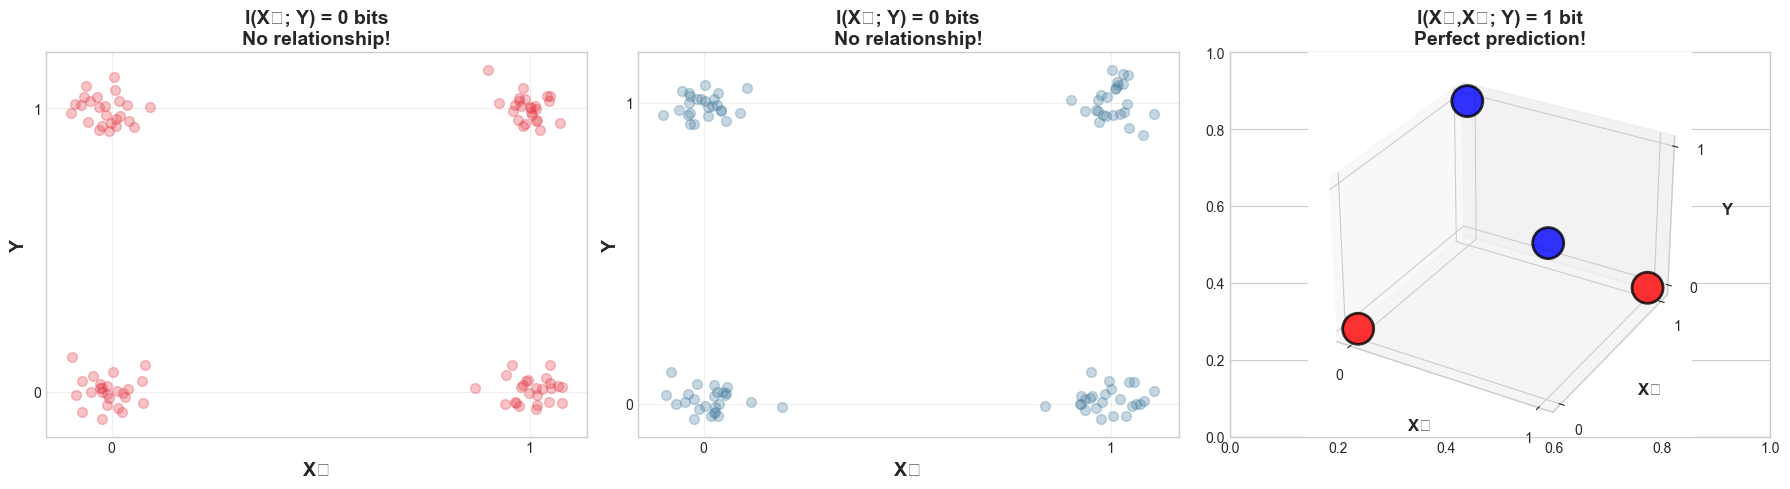
\includegraphics[keepaspectratio]{02_xor_problem_synergy_files/figure-pdf/cell-7-output-1.png}}

\begin{verbatim}

Key Insight from Visualization:
Left two panels: Complete overlap → No predictability
Right panel: Perfect separation → Complete predictability

The structure is only visible in the JOINT space!
\end{verbatim}

\section{Part 3: Why the Venn Diagram
Breaks}\label{part-3-why-the-venn-diagram-breaks}

\subsection{The Two-Variable Venn Diagram (It
Works!)}\label{the-two-variable-venn-diagram-it-works}

For two variables, we can represent information as overlapping circles.
The overlap is the mutual information.

\subsection{The Three-Variable Venn Diagram (It
Breaks!)}\label{the-three-variable-venn-diagram-it-breaks}

With three variables, we'd naively draw three overlapping circles. But
what goes in the center (the triple overlap)?

For the XOR case: - Each circle represents \(H(X_1)\), \(H(X_2)\),
\(H(Y)\) = 1 bit each - The pairwise overlaps:
\(I(X_1; Y) = I(X_2; Y) = I(X_1; X_2) = 0\) bits - But
\(I(X_1, X_2; Y) = 1\) bit!

\textbf{The Problem}: If pairwise overlaps are zero, where does this 1
bit live?

\textbf{The Answer}: It must be in the center (triple overlap). But then
we'd need:
\[\text{Center region} = I(X_1, X_2; Y) - I(X_1; Y) - I(X_2; Y) + \text{"corrections"} = 1 - 0 - 0 = 1\]

But wait\ldots{} there are \textbf{no} pairwise overlaps to ``get to''
this center!

Let's visualize this impossibility:

\begin{Shaded}
\begin{Highlighting}[]
\NormalTok{fig, (ax1, ax2) }\OperatorTok{=}\NormalTok{ plt.subplots(}\DecValTok{1}\NormalTok{, }\DecValTok{2}\NormalTok{, figsize}\OperatorTok{=}\NormalTok{(}\DecValTok{16}\NormalTok{, }\DecValTok{7}\NormalTok{))}

\CommentTok{\# Left: Standard 3{-}way Venn}
\ImportTok{from}\NormalTok{ matplotlib.patches }\ImportTok{import}\NormalTok{ Ellipse}
\NormalTok{ax1.set\_xlim(}\OperatorTok{{-}}\DecValTok{2}\NormalTok{, }\DecValTok{2}\NormalTok{)}
\NormalTok{ax1.set\_ylim(}\OperatorTok{{-}}\DecValTok{2}\NormalTok{, }\DecValTok{2}\NormalTok{)}
\NormalTok{ax1.set\_aspect(}\StringTok{\textquotesingle{}equal\textquotesingle{}}\NormalTok{)}
\NormalTok{ax1.axis(}\StringTok{\textquotesingle{}off\textquotesingle{}}\NormalTok{)}

\CommentTok{\# Draw three circles}
\NormalTok{c1 }\OperatorTok{=}\NormalTok{ Circle((}\DecValTok{0}\NormalTok{, }\FloatTok{0.5}\NormalTok{), }\FloatTok{0.8}\NormalTok{, alpha}\OperatorTok{=}\FloatTok{0.3}\NormalTok{, color}\OperatorTok{=}\StringTok{\textquotesingle{}red\textquotesingle{}}\NormalTok{, label}\OperatorTok{=}\StringTok{\textquotesingle{}H(X₁)\textquotesingle{}}\NormalTok{)}
\NormalTok{c2 }\OperatorTok{=}\NormalTok{ Circle((}\FloatTok{0.7}\NormalTok{, }\OperatorTok{{-}}\FloatTok{0.4}\NormalTok{), }\FloatTok{0.8}\NormalTok{, alpha}\OperatorTok{=}\FloatTok{0.3}\NormalTok{, color}\OperatorTok{=}\StringTok{\textquotesingle{}blue\textquotesingle{}}\NormalTok{, label}\OperatorTok{=}\StringTok{\textquotesingle{}H(X₂)\textquotesingle{}}\NormalTok{)}
\NormalTok{c3 }\OperatorTok{=}\NormalTok{ Circle((}\OperatorTok{{-}}\FloatTok{0.7}\NormalTok{, }\OperatorTok{{-}}\FloatTok{0.4}\NormalTok{), }\FloatTok{0.8}\NormalTok{, alpha}\OperatorTok{=}\FloatTok{0.3}\NormalTok{, color}\OperatorTok{=}\StringTok{\textquotesingle{}green\textquotesingle{}}\NormalTok{, label}\OperatorTok{=}\StringTok{\textquotesingle{}H(Y)\textquotesingle{}}\NormalTok{)}
\NormalTok{ax1.add\_patch(c1)}
\NormalTok{ax1.add\_patch(c2)}
\NormalTok{ax1.add\_patch(c3)}

\CommentTok{\# Label regions}
\NormalTok{ax1.text(}\DecValTok{0}\NormalTok{, }\FloatTok{0.9}\NormalTok{, }\StringTok{\textquotesingle{}H(X₁)\textquotesingle{}}\NormalTok{, ha}\OperatorTok{=}\StringTok{\textquotesingle{}center\textquotesingle{}}\NormalTok{, fontsize}\OperatorTok{=}\DecValTok{14}\NormalTok{, fontweight}\OperatorTok{=}\StringTok{\textquotesingle{}bold\textquotesingle{}}\NormalTok{)}
\NormalTok{ax1.text(}\FloatTok{0.9}\NormalTok{, }\OperatorTok{{-}}\FloatTok{0.7}\NormalTok{, }\StringTok{\textquotesingle{}H(X₂)\textquotesingle{}}\NormalTok{, ha}\OperatorTok{=}\StringTok{\textquotesingle{}center\textquotesingle{}}\NormalTok{, fontsize}\OperatorTok{=}\DecValTok{14}\NormalTok{, fontweight}\OperatorTok{=}\StringTok{\textquotesingle{}bold\textquotesingle{}}\NormalTok{)}
\NormalTok{ax1.text(}\OperatorTok{{-}}\FloatTok{0.9}\NormalTok{, }\OperatorTok{{-}}\FloatTok{0.7}\NormalTok{, }\StringTok{\textquotesingle{}H(Y)\textquotesingle{}}\NormalTok{, ha}\OperatorTok{=}\StringTok{\textquotesingle{}center\textquotesingle{}}\NormalTok{, fontsize}\OperatorTok{=}\DecValTok{14}\NormalTok{, fontweight}\OperatorTok{=}\StringTok{\textquotesingle{}bold\textquotesingle{}}\NormalTok{)}
\NormalTok{ax1.text(}\DecValTok{0}\NormalTok{, }\OperatorTok{{-}}\FloatTok{0.15}\NormalTok{, }\StringTok{\textquotesingle{}???\textquotesingle{}}\NormalTok{, ha}\OperatorTok{=}\StringTok{\textquotesingle{}center\textquotesingle{}}\NormalTok{, fontsize}\OperatorTok{=}\DecValTok{24}\NormalTok{, fontweight}\OperatorTok{=}\StringTok{\textquotesingle{}bold\textquotesingle{}}\NormalTok{, color}\OperatorTok{=}\StringTok{\textquotesingle{}red\textquotesingle{}}\NormalTok{)}
\NormalTok{ax1.text(}\DecValTok{0}\NormalTok{, }\OperatorTok{{-}}\FloatTok{0.6}\NormalTok{, }\StringTok{\textquotesingle{}Center region}\CharTok{\textbackslash{}n}\StringTok{should have}\CharTok{\textbackslash{}n}\StringTok{1 bit!\textquotesingle{}}\NormalTok{, ha}\OperatorTok{=}\StringTok{\textquotesingle{}center\textquotesingle{}}\NormalTok{, fontsize}\OperatorTok{=}\DecValTok{11}\NormalTok{,}
\NormalTok{         bbox}\OperatorTok{=}\BuiltInTok{dict}\NormalTok{(boxstyle}\OperatorTok{=}\StringTok{\textquotesingle{}round\textquotesingle{}}\NormalTok{, facecolor}\OperatorTok{=}\StringTok{\textquotesingle{}yellow\textquotesingle{}}\NormalTok{, alpha}\OperatorTok{=}\FloatTok{0.7}\NormalTok{))}

\CommentTok{\# Pairwise overlaps are 0}
\NormalTok{ax1.text(}\FloatTok{0.35}\NormalTok{, }\FloatTok{0.1}\NormalTok{, }\StringTok{\textquotesingle{}I(X₁;X₂)=0\textquotesingle{}}\NormalTok{, fontsize}\OperatorTok{=}\DecValTok{10}\NormalTok{, rotation}\OperatorTok{={-}}\DecValTok{30}\NormalTok{)}
\NormalTok{ax1.text(}\OperatorTok{{-}}\FloatTok{0.35}\NormalTok{, }\FloatTok{0.1}\NormalTok{, }\StringTok{\textquotesingle{}I(X₁;Y)=0\textquotesingle{}}\NormalTok{, fontsize}\OperatorTok{=}\DecValTok{10}\NormalTok{, rotation}\OperatorTok{=}\DecValTok{30}\NormalTok{)}
\NormalTok{ax1.text(}\DecValTok{0}\NormalTok{, }\OperatorTok{{-}}\FloatTok{0.85}\NormalTok{, }\StringTok{\textquotesingle{}I(X₂;Y)=0\textquotesingle{}}\NormalTok{, fontsize}\OperatorTok{=}\DecValTok{10}\NormalTok{)}

\NormalTok{ax1.set\_title(}\StringTok{\textquotesingle{}IMPOSSIBLE Venn Diagram for XOR\textquotesingle{}}\NormalTok{, fontsize}\OperatorTok{=}\DecValTok{16}\NormalTok{, fontweight}\OperatorTok{=}\StringTok{\textquotesingle{}bold\textquotesingle{}}\NormalTok{, pad}\OperatorTok{=}\DecValTok{20}\NormalTok{)}
\NormalTok{ax1.legend(loc}\OperatorTok{=}\StringTok{\textquotesingle{}upper right\textquotesingle{}}\NormalTok{, fontsize}\OperatorTok{=}\DecValTok{11}\NormalTok{)}

\CommentTok{\# Right: The truth {-} information structure}
\NormalTok{ax2.set\_xlim(}\DecValTok{0}\NormalTok{, }\DecValTok{4}\NormalTok{)}
\NormalTok{ax2.set\_ylim(}\DecValTok{0}\NormalTok{, }\DecValTok{4}\NormalTok{)}
\NormalTok{ax2.axis(}\StringTok{\textquotesingle{}off\textquotesingle{}}\NormalTok{)}

\CommentTok{\# Draw boxes for each variable\textquotesingle{}s entropy}
\NormalTok{box1 }\OperatorTok{=}\NormalTok{ FancyBboxPatch((}\FloatTok{0.2}\NormalTok{, }\FloatTok{2.5}\NormalTok{), }\FloatTok{1.2}\NormalTok{, }\DecValTok{1}\NormalTok{, boxstyle}\OperatorTok{=}\StringTok{"round,pad=0.05"}\NormalTok{, }
\NormalTok{                       edgecolor}\OperatorTok{=}\StringTok{\textquotesingle{}red\textquotesingle{}}\NormalTok{, facecolor}\OperatorTok{=}\StringTok{\textquotesingle{}red\textquotesingle{}}\NormalTok{, alpha}\OperatorTok{=}\FloatTok{0.3}\NormalTok{, linewidth}\OperatorTok{=}\DecValTok{3}\NormalTok{)}
\NormalTok{box2 }\OperatorTok{=}\NormalTok{ FancyBboxPatch((}\FloatTok{1.5}\NormalTok{, }\FloatTok{2.5}\NormalTok{), }\FloatTok{1.2}\NormalTok{, }\DecValTok{1}\NormalTok{, boxstyle}\OperatorTok{=}\StringTok{"round,pad=0.05"}\NormalTok{,}
\NormalTok{                       edgecolor}\OperatorTok{=}\StringTok{\textquotesingle{}blue\textquotesingle{}}\NormalTok{, facecolor}\OperatorTok{=}\StringTok{\textquotesingle{}blue\textquotesingle{}}\NormalTok{, alpha}\OperatorTok{=}\FloatTok{0.3}\NormalTok{, linewidth}\OperatorTok{=}\DecValTok{3}\NormalTok{)}
\NormalTok{box3 }\OperatorTok{=}\NormalTok{ FancyBboxPatch((}\FloatTok{2.8}\NormalTok{, }\FloatTok{2.5}\NormalTok{), }\FloatTok{1.2}\NormalTok{, }\DecValTok{1}\NormalTok{, boxstyle}\OperatorTok{=}\StringTok{"round,pad=0.05"}\NormalTok{,}
\NormalTok{                       edgecolor}\OperatorTok{=}\StringTok{\textquotesingle{}green\textquotesingle{}}\NormalTok{, facecolor}\OperatorTok{=}\StringTok{\textquotesingle{}green\textquotesingle{}}\NormalTok{, alpha}\OperatorTok{=}\FloatTok{0.3}\NormalTok{, linewidth}\OperatorTok{=}\DecValTok{3}\NormalTok{)}
\NormalTok{ax2.add\_patch(box1)}
\NormalTok{ax2.add\_patch(box2)}
\NormalTok{ax2.add\_patch(box3)}

\NormalTok{ax2.text(}\FloatTok{0.8}\NormalTok{, }\DecValTok{3}\NormalTok{, }\StringTok{\textquotesingle{}X₁}\CharTok{\textbackslash{}n}\StringTok{1 bit\textquotesingle{}}\NormalTok{, ha}\OperatorTok{=}\StringTok{\textquotesingle{}center\textquotesingle{}}\NormalTok{, va}\OperatorTok{=}\StringTok{\textquotesingle{}center\textquotesingle{}}\NormalTok{, fontsize}\OperatorTok{=}\DecValTok{13}\NormalTok{, fontweight}\OperatorTok{=}\StringTok{\textquotesingle{}bold\textquotesingle{}}\NormalTok{)}
\NormalTok{ax2.text(}\FloatTok{2.1}\NormalTok{, }\DecValTok{3}\NormalTok{, }\StringTok{\textquotesingle{}X₂}\CharTok{\textbackslash{}n}\StringTok{1 bit\textquotesingle{}}\NormalTok{, ha}\OperatorTok{=}\StringTok{\textquotesingle{}center\textquotesingle{}}\NormalTok{, va}\OperatorTok{=}\StringTok{\textquotesingle{}center\textquotesingle{}}\NormalTok{, fontsize}\OperatorTok{=}\DecValTok{13}\NormalTok{, fontweight}\OperatorTok{=}\StringTok{\textquotesingle{}bold\textquotesingle{}}\NormalTok{)}
\NormalTok{ax2.text(}\FloatTok{3.4}\NormalTok{, }\DecValTok{3}\NormalTok{, }\StringTok{\textquotesingle{}Y}\CharTok{\textbackslash{}n}\StringTok{1 bit\textquotesingle{}}\NormalTok{, ha}\OperatorTok{=}\StringTok{\textquotesingle{}center\textquotesingle{}}\NormalTok{, va}\OperatorTok{=}\StringTok{\textquotesingle{}center\textquotesingle{}}\NormalTok{, fontsize}\OperatorTok{=}\DecValTok{13}\NormalTok{, fontweight}\OperatorTok{=}\StringTok{\textquotesingle{}bold\textquotesingle{}}\NormalTok{)}

\CommentTok{\# Draw synergy region}
\NormalTok{synergy\_box }\OperatorTok{=}\NormalTok{ FancyBboxPatch((}\FloatTok{0.8}\NormalTok{, }\FloatTok{0.5}\NormalTok{), }\FloatTok{2.4}\NormalTok{, }\FloatTok{1.2}\NormalTok{, boxstyle}\OperatorTok{=}\StringTok{"round,pad=0.05"}\NormalTok{,}
\NormalTok{                              edgecolor}\OperatorTok{=}\StringTok{\textquotesingle{}purple\textquotesingle{}}\NormalTok{, facecolor}\OperatorTok{=}\StringTok{\textquotesingle{}purple\textquotesingle{}}\NormalTok{, }
\NormalTok{                              alpha}\OperatorTok{=}\FloatTok{0.5}\NormalTok{, linewidth}\OperatorTok{=}\DecValTok{4}\NormalTok{, linestyle}\OperatorTok{=}\StringTok{\textquotesingle{}dashed\textquotesingle{}}\NormalTok{)}
\NormalTok{ax2.add\_patch(synergy\_box)}
\NormalTok{ax2.text(}\DecValTok{2}\NormalTok{, }\FloatTok{1.1}\NormalTok{, }\StringTok{\textquotesingle{}SYNERGY}\CharTok{\textbackslash{}n}\StringTok{1 bit}\CharTok{\textbackslash{}n}\StringTok{(requires ALL THREE)\textquotesingle{}}\NormalTok{, ha}\OperatorTok{=}\StringTok{\textquotesingle{}center\textquotesingle{}}\NormalTok{, va}\OperatorTok{=}\StringTok{\textquotesingle{}center\textquotesingle{}}\NormalTok{,}
\NormalTok{         fontsize}\OperatorTok{=}\DecValTok{13}\NormalTok{, fontweight}\OperatorTok{=}\StringTok{\textquotesingle{}bold\textquotesingle{}}\NormalTok{, color}\OperatorTok{=}\StringTok{\textquotesingle{}white\textquotesingle{}}\NormalTok{,}
\NormalTok{         bbox}\OperatorTok{=}\BuiltInTok{dict}\NormalTok{(boxstyle}\OperatorTok{=}\StringTok{\textquotesingle{}round\textquotesingle{}}\NormalTok{, facecolor}\OperatorTok{=}\StringTok{\textquotesingle{}purple\textquotesingle{}}\NormalTok{, alpha}\OperatorTok{=}\FloatTok{0.8}\NormalTok{))}

\CommentTok{\# Draw arrows}
\NormalTok{arrow1 }\OperatorTok{=}\NormalTok{ FancyArrowPatch((}\FloatTok{0.8}\NormalTok{, }\FloatTok{2.4}\NormalTok{), (}\FloatTok{1.3}\NormalTok{, }\FloatTok{1.8}\NormalTok{), }
\NormalTok{                         arrowstyle}\OperatorTok{=}\StringTok{\textquotesingle{}{-}\textgreater{}\textquotesingle{}}\NormalTok{, mutation\_scale}\OperatorTok{=}\DecValTok{30}\NormalTok{, linewidth}\OperatorTok{=}\DecValTok{3}\NormalTok{, color}\OperatorTok{=}\StringTok{\textquotesingle{}purple\textquotesingle{}}\NormalTok{)}
\NormalTok{arrow2 }\OperatorTok{=}\NormalTok{ FancyArrowPatch((}\FloatTok{2.1}\NormalTok{, }\FloatTok{2.4}\NormalTok{), (}\DecValTok{2}\NormalTok{, }\FloatTok{1.8}\NormalTok{),}
\NormalTok{                         arrowstyle}\OperatorTok{=}\StringTok{\textquotesingle{}{-}\textgreater{}\textquotesingle{}}\NormalTok{, mutation\_scale}\OperatorTok{=}\DecValTok{30}\NormalTok{, linewidth}\OperatorTok{=}\DecValTok{3}\NormalTok{, color}\OperatorTok{=}\StringTok{\textquotesingle{}purple\textquotesingle{}}\NormalTok{)}
\NormalTok{arrow3 }\OperatorTok{=}\NormalTok{ FancyArrowPatch((}\FloatTok{3.4}\NormalTok{, }\FloatTok{2.4}\NormalTok{), (}\FloatTok{2.7}\NormalTok{, }\FloatTok{1.8}\NormalTok{),}
\NormalTok{                         arrowstyle}\OperatorTok{=}\StringTok{\textquotesingle{}{-}\textgreater{}\textquotesingle{}}\NormalTok{, mutation\_scale}\OperatorTok{=}\DecValTok{30}\NormalTok{, linewidth}\OperatorTok{=}\DecValTok{3}\NormalTok{, color}\OperatorTok{=}\StringTok{\textquotesingle{}purple\textquotesingle{}}\NormalTok{)}
\NormalTok{ax2.add\_patch(arrow1)}
\NormalTok{ax2.add\_patch(arrow2)}
\NormalTok{ax2.add\_patch(arrow3)}

\NormalTok{ax2.set\_title(}\StringTok{\textquotesingle{}The ACTUAL Information Structure\textquotesingle{}}\NormalTok{, fontsize}\OperatorTok{=}\DecValTok{16}\NormalTok{, fontweight}\OperatorTok{=}\StringTok{\textquotesingle{}bold\textquotesingle{}}\NormalTok{, pad}\OperatorTok{=}\DecValTok{20}\NormalTok{)}

\NormalTok{plt.tight\_layout()}
\NormalTok{plt.show()}

\BuiltInTok{print}\NormalTok{(}\StringTok{"}\CharTok{\textbackslash{}n}\StringTok{🚨 CRITICAL INSIGHT:"}\NormalTok{)}
\BuiltInTok{print}\NormalTok{(}\StringTok{"="} \OperatorTok{*} \DecValTok{60}\NormalTok{)}
\BuiltInTok{print}\NormalTok{(}\StringTok{"Venn diagrams ONLY work for 2 variables!"}\NormalTok{)}
\BuiltInTok{print}\NormalTok{(}\StringTok{"}\CharTok{\textbackslash{}n}\StringTok{For 3+ variables, we need a different framework:"}\NormalTok{)}
\BuiltInTok{print}\NormalTok{(}\StringTok{"  → Interaction Information (can be negative!)"}\NormalTok{)}
\BuiltInTok{print}\NormalTok{(}\StringTok{"  → Partial Information Decomposition (PID)"}\NormalTok{)}
\BuiltInTok{print}\NormalTok{(}\StringTok{"}\CharTok{\textbackslash{}n}\StringTok{These are what HOI package implements! (Next notebook)"}\NormalTok{)}
\end{Highlighting}
\end{Shaded}

\pandocbounded{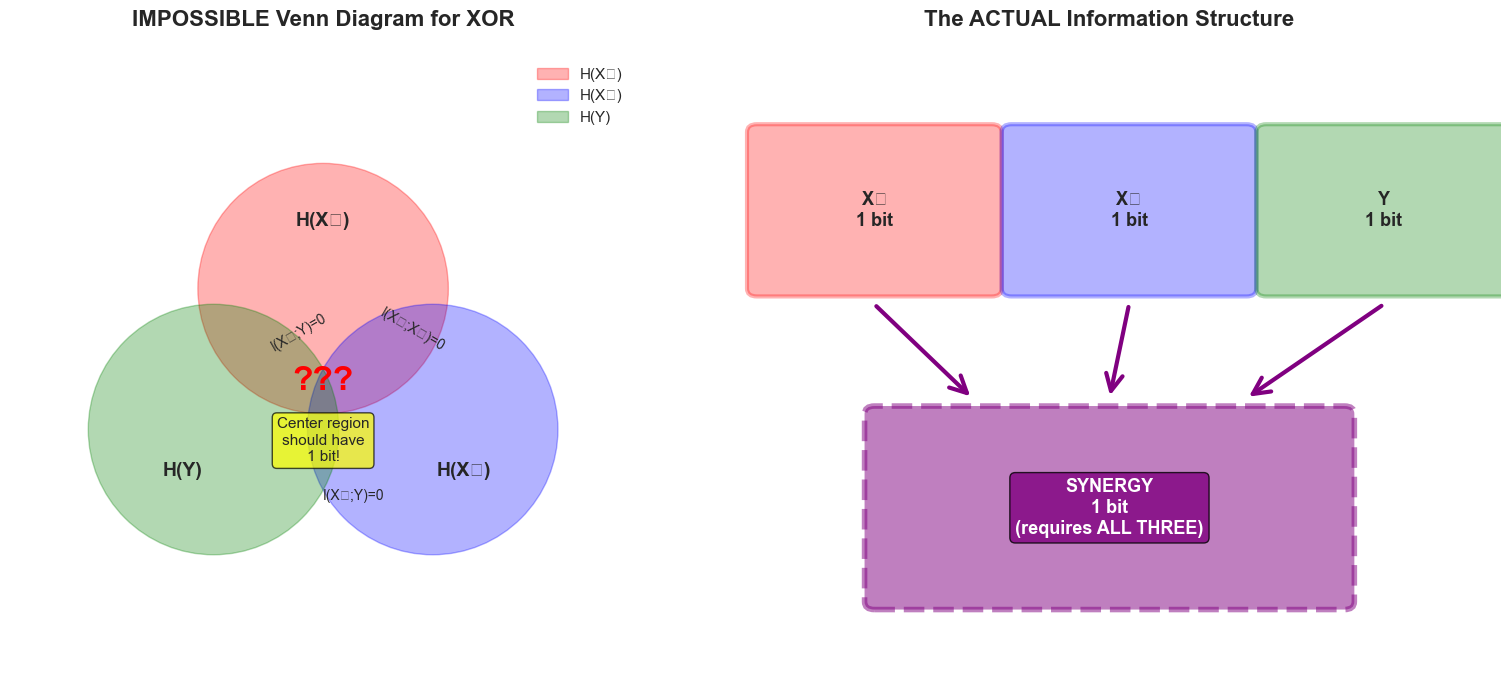
\includegraphics[keepaspectratio]{02_xor_problem_synergy_files/figure-pdf/cell-8-output-1.png}}

\begin{verbatim}

🚨 CRITICAL INSIGHT:
============================================================
Venn diagrams ONLY work for 2 variables!

For 3+ variables, we need a different framework:
  → Interaction Information (can be negative!)
  → Partial Information Decomposition (PID)

These are what HOI package implements! (Next notebook)
\end{verbatim}

\section{Part 4: Interaction
Information}\label{part-4-interaction-information}

\subsection{The Solution: A Signed
Measure}\label{the-solution-a-signed-measure}

\textbf{Interaction Information} for three variables is defined as:

\[I(X_1; X_2; Y) = I(X_1; X_2) - I(X_1; X_2 | Y)\]

Alternatively: \[I(X_1; X_2; Y) = I(X_1; Y) - I(X_1; Y | X_2)\]

Or in the \textbf{surprise form}:
\[I(X_1; X_2; Y) = I(X_1; Y) + I(X_2; Y) + I(X_1; X_2) - I(X_1, X_2; Y)\]

\subsection{Key Property: Can Be
Negative!}\label{key-property-can-be-negative}

Unlike mutual information (always ≥ 0), interaction information can be:
- \textbf{Positive}: Redundancy (common cause structure) -
\textbf{Zero}: No higher-order interaction - \textbf{Negative}: Synergy
(XOR-like structure)

\subsection{For XOR, Interaction Information is
Negative}\label{for-xor-interaction-information-is-negative}

\begin{Shaded}
\begin{Highlighting}[]
\KeywordTok{def}\NormalTok{ interaction\_information(P\_XYZ):}
    \CommentTok{"""}
\CommentTok{    Calculate interaction information I(X;Y;Z).}
\CommentTok{    }
\CommentTok{    Using: I(X;Y;Z) = I(X;Y) + I(X;Z) + I(Y;Z) {-} I(X;YZ) {-} I(Y;XZ) {-} I(Z;XY) + I(X;Y;Z)}
\CommentTok{    }
\CommentTok{    Simplified form:}
\CommentTok{    I(X;Y;Z) = I(X;Y) {-} I(X;Y|Z)}
\CommentTok{    }
\CommentTok{    Convention: Negative means synergy (as in XOR)}
\CommentTok{    """}
    \CommentTok{\# Get all pairwise MIs}
\NormalTok{    P\_X\_Y }\OperatorTok{=}\NormalTok{ P\_XYZ.}\BuiltInTok{sum}\NormalTok{(axis}\OperatorTok{=}\DecValTok{1}\NormalTok{)  }\CommentTok{\# Marginalize Z}
\NormalTok{    P\_X\_Z }\OperatorTok{=}\NormalTok{ P\_XYZ.}\BuiltInTok{sum}\NormalTok{(axis}\OperatorTok{=}\DecValTok{2}\NormalTok{).T  }\CommentTok{\# Marginalize Y and transpose}
\NormalTok{    P\_Y\_Z }\OperatorTok{=}\NormalTok{ P\_XYZ.}\BuiltInTok{sum}\NormalTok{(axis}\OperatorTok{=}\DecValTok{0}\NormalTok{)  }\CommentTok{\# Marginalize X}
    
\NormalTok{    I\_XY }\OperatorTok{=}\NormalTok{ mutual\_information(P\_X\_Y)}
\NormalTok{    I\_XZ }\OperatorTok{=}\NormalTok{ mutual\_information(P\_X\_Z)}
\NormalTok{    I\_YZ }\OperatorTok{=}\NormalTok{ mutual\_information(P\_Y\_Z)}
    
    \CommentTok{\# Get three{-}way MI}
\NormalTok{    I\_XYZ }\OperatorTok{=}\NormalTok{ joint\_mi\_three\_vars(P\_XYZ)}
    
    \CommentTok{\# Interaction information}
\NormalTok{    II }\OperatorTok{=}\NormalTok{ I\_XY }\OperatorTok{+}\NormalTok{ I\_XZ }\OperatorTok{+}\NormalTok{ I\_YZ }\OperatorTok{{-}}\NormalTok{ I\_XYZ}
    
    \ControlFlowTok{return}\NormalTok{ II}

\CommentTok{\# Calculate for XOR}
\NormalTok{II\_XOR }\OperatorTok{=}\NormalTok{ interaction\_information(P\_XOR)}

\BuiltInTok{print}\NormalTok{(}\StringTok{"Interaction Information for XOR"}\NormalTok{)}
\BuiltInTok{print}\NormalTok{(}\StringTok{"="} \OperatorTok{*} \DecValTok{60}\NormalTok{)}
\BuiltInTok{print}\NormalTok{(}\SpecialStringTok{f"}\CharTok{\textbackslash{}n}\SpecialStringTok{I(X₁; X₂; Y) = }\SpecialCharTok{\{}\NormalTok{II\_XOR}\SpecialCharTok{:.4f\}}\SpecialStringTok{ bits"}\NormalTok{)}

\ControlFlowTok{if}\NormalTok{ II\_XOR }\OperatorTok{\textless{}} \DecValTok{0}\NormalTok{:}
    \BuiltInTok{print}\NormalTok{(}\StringTok{"}\CharTok{\textbackslash{}n}\StringTok{✅ NEGATIVE! This indicates SYNERGY."}\NormalTok{)}
    \BuiltInTok{print}\NormalTok{(}\StringTok{"}\CharTok{\textbackslash{}n}\StringTok{Interpretation:"}\NormalTok{)}
    \BuiltInTok{print}\NormalTok{(}\StringTok{"  The three variables together have LESS pairwise structure"}\NormalTok{)}
    \BuiltInTok{print}\NormalTok{(}\StringTok{"  than you\textquotesingle{}d expect from their marginals."}\NormalTok{)}
    \BuiltInTok{print}\NormalTok{(}\StringTok{"  The information is \textquotesingle{}hidden\textquotesingle{} in the triple interaction!"}\NormalTok{)}
    
\CommentTok{\# Let\textquotesingle{}s verify the calculation}
\BuiltInTok{print}\NormalTok{(}\StringTok{"}\CharTok{\textbackslash{}n}\StringTok{"} \OperatorTok{+} \StringTok{"="} \OperatorTok{*} \DecValTok{60}\NormalTok{)}
\BuiltInTok{print}\NormalTok{(}\StringTok{"Verification using alternative form:"}\NormalTok{)}
\BuiltInTok{print}\NormalTok{(}\StringTok{"I(X₁; X₂; Y) = I(X₁;Y) + I(X₂;Y) + I(X₁;X₂) {-} I(X₁,X₂;Y)"}\NormalTok{)}
\BuiltInTok{print}\NormalTok{(}\SpecialStringTok{f"            = }\SpecialCharTok{\{}\NormalTok{MI\_X1\_Y}\SpecialCharTok{:.1f\}}\SpecialStringTok{ + }\SpecialCharTok{\{}\NormalTok{MI\_X2\_Y}\SpecialCharTok{:.1f\}}\SpecialStringTok{ + 0 {-} }\SpecialCharTok{\{}\NormalTok{MI\_X1X2\_Y}\SpecialCharTok{:.1f\}}\SpecialStringTok{"}\NormalTok{)}
\BuiltInTok{print}\NormalTok{(}\SpecialStringTok{f"            = }\SpecialCharTok{\{}\NormalTok{MI\_X1\_Y }\OperatorTok{+}\NormalTok{ MI\_X2\_Y }\OperatorTok{+} \DecValTok{0} \OperatorTok{{-}}\NormalTok{ MI\_X1X2\_Y}\SpecialCharTok{:.4f\}}\SpecialStringTok{ bits ✓"}\NormalTok{)}
\end{Highlighting}
\end{Shaded}

\begin{verbatim}
Interaction Information for XOR
============================================================

I(X₁; X₂; Y) = -1.0000 bits

✅ NEGATIVE! This indicates SYNERGY.

Interpretation:
  The three variables together have LESS pairwise structure
  than you'd expect from their marginals.
  The information is 'hidden' in the triple interaction!

============================================================
Verification using alternative form:
I(X₁; X₂; Y) = I(X₁;Y) + I(X₂;Y) + I(X₁;X₂) - I(X₁,X₂;Y)
            = 0.0 + 0.0 + 0 - 1.0
            = -1.0000 bits ✓
\end{verbatim}

\subsection{Interpreting the Sign of Interaction
Information}\label{interpreting-the-sign-of-interaction-information}

Let's create examples of all three cases to build intuition:

\begin{Shaded}
\begin{Highlighting}[]
\CommentTok{\# Case 1: XOR (Synergy) {-} We already have this}
\NormalTok{II\_synergy }\OperatorTok{=}\NormalTok{ II\_XOR}

\CommentTok{\# Case 2: Common cause (Redundancy)}
\CommentTok{\# Z causes both X and Y}
\NormalTok{P\_redundancy }\OperatorTok{=}\NormalTok{ np.zeros((}\DecValTok{2}\NormalTok{, }\DecValTok{2}\NormalTok{, }\DecValTok{2}\NormalTok{))}
\CommentTok{\# When Z=0: X=0, Y=0 with high prob}
\NormalTok{P\_redundancy[}\DecValTok{0}\NormalTok{, }\DecValTok{0}\NormalTok{, }\DecValTok{0}\NormalTok{] }\OperatorTok{=} \FloatTok{0.4}
\NormalTok{P\_redundancy[}\DecValTok{1}\NormalTok{, }\DecValTok{0}\NormalTok{, }\DecValTok{0}\NormalTok{] }\OperatorTok{=} \FloatTok{0.05}
\NormalTok{P\_redundancy[}\DecValTok{0}\NormalTok{, }\DecValTok{1}\NormalTok{, }\DecValTok{0}\NormalTok{] }\OperatorTok{=} \FloatTok{0.05}
\CommentTok{\# When Z=1: X=1, Y=1 with high prob  }
\NormalTok{P\_redundancy[}\DecValTok{1}\NormalTok{, }\DecValTok{1}\NormalTok{, }\DecValTok{1}\NormalTok{] }\OperatorTok{=} \FloatTok{0.4}
\NormalTok{P\_redundancy[}\DecValTok{0}\NormalTok{, }\DecValTok{1}\NormalTok{, }\DecValTok{1}\NormalTok{] }\OperatorTok{=} \FloatTok{0.05}
\NormalTok{P\_redundancy[}\DecValTok{1}\NormalTok{, }\DecValTok{0}\NormalTok{, }\DecValTok{1}\NormalTok{] }\OperatorTok{=} \FloatTok{0.05}

\NormalTok{II\_redundancy }\OperatorTok{=}\NormalTok{ interaction\_information(P\_redundancy)}

\CommentTok{\# Case 3: Independent (No interaction)}
\NormalTok{P\_independent }\OperatorTok{=}\NormalTok{ np.zeros((}\DecValTok{2}\NormalTok{, }\DecValTok{2}\NormalTok{, }\DecValTok{2}\NormalTok{))}
\ControlFlowTok{for}\NormalTok{ i, j, k }\KeywordTok{in}\NormalTok{ product([}\DecValTok{0}\NormalTok{, }\DecValTok{1}\NormalTok{], repeat}\OperatorTok{=}\DecValTok{3}\NormalTok{):}
\NormalTok{    P\_independent[i, j, k] }\OperatorTok{=} \FloatTok{0.125}  \CommentTok{\# All equally likely}

\NormalTok{II\_independent }\OperatorTok{=}\NormalTok{ interaction\_information(P\_independent)}

\CommentTok{\# Display results}
\BuiltInTok{print}\NormalTok{(}\StringTok{"Comparison of Interaction Information"}\NormalTok{)}
\BuiltInTok{print}\NormalTok{(}\StringTok{"="} \OperatorTok{*} \DecValTok{60}\NormalTok{)}
\BuiltInTok{print}\NormalTok{(}\StringTok{"}\CharTok{\textbackslash{}n}\StringTok{1. XOR (Pure Synergy):"}\NormalTok{)}
\BuiltInTok{print}\NormalTok{(}\SpecialStringTok{f"   I(X₁; X₂; Y) = }\SpecialCharTok{\{}\NormalTok{II\_synergy}\SpecialCharTok{:.4f\}}\SpecialStringTok{ bits (NEGATIVE)"}\NormalTok{)}
\BuiltInTok{print}\NormalTok{(}\StringTok{"   → Information emerges from combination"}\NormalTok{)}
\BuiltInTok{print}\NormalTok{(}\StringTok{"   → Neither variable alone helps"}\NormalTok{)}

\BuiltInTok{print}\NormalTok{(}\StringTok{"}\CharTok{\textbackslash{}n}\StringTok{2. Common Cause (Redundancy):"}\NormalTok{)}
\BuiltInTok{print}\NormalTok{(}\SpecialStringTok{f"   I(X₁; X₂; Y) = }\SpecialCharTok{\{}\NormalTok{II\_redundancy}\SpecialCharTok{:.4f\}}\SpecialStringTok{ bits (POSITIVE)"}\NormalTok{)}
\BuiltInTok{print}\NormalTok{(}\StringTok{"   → Variables carry overlapping information"}\NormalTok{)}
\BuiltInTok{print}\NormalTok{(}\StringTok{"   → Learning one reduces value of the other"}\NormalTok{)}

\BuiltInTok{print}\NormalTok{(}\StringTok{"}\CharTok{\textbackslash{}n}\StringTok{3. Independent Variables:"}\NormalTok{)}
\BuiltInTok{print}\NormalTok{(}\SpecialStringTok{f"   I(X₁; X₂; Y) = }\SpecialCharTok{\{}\NormalTok{II\_independent}\SpecialCharTok{:.6f\}}\SpecialStringTok{ bits (≈ ZERO)"}\NormalTok{)}
\BuiltInTok{print}\NormalTok{(}\StringTok{"   → No higher{-}order structure"}\NormalTok{)}
\BuiltInTok{print}\NormalTok{(}\StringTok{"   → Pairwise analysis is sufficient"}\NormalTok{)}

\BuiltInTok{print}\NormalTok{(}\StringTok{"}\CharTok{\textbackslash{}n}\StringTok{"} \OperatorTok{+} \StringTok{"="} \OperatorTok{*} \DecValTok{60}\NormalTok{)}
\BuiltInTok{print}\NormalTok{(}\StringTok{"Key Insight: The SIGN tells you the information structure!"}\NormalTok{)}
\end{Highlighting}
\end{Shaded}

\begin{verbatim}
Comparison of Interaction Information
============================================================

1. XOR (Pure Synergy):
   I(X₁; X₂; Y) = -1.0000 bits (NEGATIVE)
   → Information emerges from combination
   → Neither variable alone helps

2. Common Cause (Redundancy):
   I(X₁; X₂; Y) = 0.5401 bits (POSITIVE)
   → Variables carry overlapping information
   → Learning one reduces value of the other

3. Independent Variables:
   I(X₁; X₂; Y) = 0.000000 bits (≈ ZERO)
   → No higher-order structure
   → Pairwise analysis is sufficient

============================================================
Key Insight: The SIGN tells you the information structure!
\end{verbatim}

\subsection{Visualizing Interaction Information Across
Structures}\label{visualizing-interaction-information-across-structures}

\begin{Shaded}
\begin{Highlighting}[]
\NormalTok{fig, axes }\OperatorTok{=}\NormalTok{ plt.subplots(}\DecValTok{1}\NormalTok{, }\DecValTok{3}\NormalTok{, figsize}\OperatorTok{=}\NormalTok{(}\DecValTok{18}\NormalTok{, }\DecValTok{5}\NormalTok{))}

\NormalTok{structures }\OperatorTok{=}\NormalTok{ [}
\NormalTok{    (}\StringTok{\textquotesingle{}XOR}\CharTok{\textbackslash{}n}\StringTok{(Synergy)\textquotesingle{}}\NormalTok{, II\_synergy, }\StringTok{\textquotesingle{}purple\textquotesingle{}}\NormalTok{),}
\NormalTok{    (}\StringTok{\textquotesingle{}Independent}\CharTok{\textbackslash{}n}\StringTok{(No Interaction)\textquotesingle{}}\NormalTok{, II\_independent, }\StringTok{\textquotesingle{}gray\textquotesingle{}}\NormalTok{),}
\NormalTok{    (}\StringTok{\textquotesingle{}Common Cause}\CharTok{\textbackslash{}n}\StringTok{(Redundancy)\textquotesingle{}}\NormalTok{, II\_redundancy, }\StringTok{\textquotesingle{}orange\textquotesingle{}}\NormalTok{)}
\NormalTok{]}

\ControlFlowTok{for}\NormalTok{ idx, (name, value, color) }\KeywordTok{in} \BuiltInTok{enumerate}\NormalTok{(structures):}
\NormalTok{    ax }\OperatorTok{=}\NormalTok{ axes[idx]}
    
    \CommentTok{\# Bar plot}
\NormalTok{    bar }\OperatorTok{=}\NormalTok{ ax.bar([}\DecValTok{0}\NormalTok{], [value], color}\OperatorTok{=}\NormalTok{color, alpha}\OperatorTok{=}\FloatTok{0.7}\NormalTok{, width}\OperatorTok{=}\FloatTok{0.5}\NormalTok{, edgecolor}\OperatorTok{=}\StringTok{\textquotesingle{}black\textquotesingle{}}\NormalTok{, linewidth}\OperatorTok{=}\DecValTok{2}\NormalTok{)}
\NormalTok{    ax.axhline(y}\OperatorTok{=}\DecValTok{0}\NormalTok{, color}\OperatorTok{=}\StringTok{\textquotesingle{}black\textquotesingle{}}\NormalTok{, linestyle}\OperatorTok{=}\StringTok{\textquotesingle{}{-}\textquotesingle{}}\NormalTok{, linewidth}\OperatorTok{=}\DecValTok{2}\NormalTok{)}
\NormalTok{    ax.set\_ylim(}\OperatorTok{{-}}\FloatTok{1.2}\NormalTok{, }\FloatTok{0.5}\NormalTok{)}
\NormalTok{    ax.set\_xlim(}\OperatorTok{{-}}\FloatTok{0.5}\NormalTok{, }\FloatTok{0.5}\NormalTok{)}
\NormalTok{    ax.set\_xticks([])}
\NormalTok{    ax.set\_ylabel(}\StringTok{\textquotesingle{}Interaction Information (bits)\textquotesingle{}}\NormalTok{, fontsize}\OperatorTok{=}\DecValTok{12}\NormalTok{, fontweight}\OperatorTok{=}\StringTok{\textquotesingle{}bold\textquotesingle{}}\NormalTok{)}
\NormalTok{    ax.set\_title(name, fontsize}\OperatorTok{=}\DecValTok{14}\NormalTok{, fontweight}\OperatorTok{=}\StringTok{\textquotesingle{}bold\textquotesingle{}}\NormalTok{)}
    
    \CommentTok{\# Add value label}
\NormalTok{    y\_pos }\OperatorTok{=}\NormalTok{ value }\OperatorTok{+}\NormalTok{ (}\FloatTok{0.05} \ControlFlowTok{if}\NormalTok{ value }\OperatorTok{\textgreater{}} \DecValTok{0} \ControlFlowTok{else} \OperatorTok{{-}}\FloatTok{0.15}\NormalTok{)}
\NormalTok{    ax.text(}\DecValTok{0}\NormalTok{, y\_pos, }\SpecialStringTok{f\textquotesingle{}}\SpecialCharTok{\{}\NormalTok{value}\SpecialCharTok{:.3f\}}\CharTok{\textbackslash{}n}\SpecialStringTok{bits\textquotesingle{}}\NormalTok{, ha}\OperatorTok{=}\StringTok{\textquotesingle{}center\textquotesingle{}}\NormalTok{, va}\OperatorTok{=}\StringTok{\textquotesingle{}bottom\textquotesingle{}} \ControlFlowTok{if}\NormalTok{ value }\OperatorTok{\textgreater{}} \DecValTok{0} \ControlFlowTok{else} \StringTok{\textquotesingle{}top\textquotesingle{}}\NormalTok{,}
\NormalTok{            fontsize}\OperatorTok{=}\DecValTok{12}\NormalTok{, fontweight}\OperatorTok{=}\StringTok{\textquotesingle{}bold\textquotesingle{}}\NormalTok{,}
\NormalTok{            bbox}\OperatorTok{=}\BuiltInTok{dict}\NormalTok{(boxstyle}\OperatorTok{=}\StringTok{\textquotesingle{}round\textquotesingle{}}\NormalTok{, facecolor}\OperatorTok{=}\StringTok{\textquotesingle{}white\textquotesingle{}}\NormalTok{, alpha}\OperatorTok{=}\FloatTok{0.8}\NormalTok{))}
    
    \CommentTok{\# Add interpretation}
    \ControlFlowTok{if}\NormalTok{ value }\OperatorTok{\textless{}} \OperatorTok{{-}}\FloatTok{0.5}\NormalTok{:}
\NormalTok{        interpretation }\OperatorTok{=} \StringTok{\textquotesingle{}Strong}\CharTok{\textbackslash{}n}\StringTok{Synergy\textquotesingle{}}
\NormalTok{        y\_text }\OperatorTok{=} \OperatorTok{{-}}\FloatTok{0.9}
    \ControlFlowTok{elif}\NormalTok{ value }\OperatorTok{\textgreater{}} \FloatTok{0.1}\NormalTok{:}
\NormalTok{        interpretation }\OperatorTok{=} \StringTok{\textquotesingle{}Redundant}\CharTok{\textbackslash{}n}\StringTok{Information\textquotesingle{}}
\NormalTok{        y\_text }\OperatorTok{=} \OperatorTok{{-}}\FloatTok{0.9}
    \ControlFlowTok{else}\NormalTok{:}
\NormalTok{        interpretation }\OperatorTok{=} \StringTok{\textquotesingle{}No Higher{-}Order}\CharTok{\textbackslash{}n}\StringTok{Structure\textquotesingle{}}
\NormalTok{        y\_text }\OperatorTok{=} \OperatorTok{{-}}\FloatTok{0.9}
    
\NormalTok{    ax.text(}\DecValTok{0}\NormalTok{, y\_text, interpretation, ha}\OperatorTok{=}\StringTok{\textquotesingle{}center\textquotesingle{}}\NormalTok{, fontsize}\OperatorTok{=}\DecValTok{11}\NormalTok{, style}\OperatorTok{=}\StringTok{\textquotesingle{}italic\textquotesingle{}}\NormalTok{,}
\NormalTok{            bbox}\OperatorTok{=}\BuiltInTok{dict}\NormalTok{(boxstyle}\OperatorTok{=}\StringTok{\textquotesingle{}round\textquotesingle{}}\NormalTok{, facecolor}\OperatorTok{=}\StringTok{\textquotesingle{}lightyellow\textquotesingle{}}\NormalTok{, alpha}\OperatorTok{=}\FloatTok{0.8}\NormalTok{))}
    
\NormalTok{    ax.grid(}\VariableTok{True}\NormalTok{, alpha}\OperatorTok{=}\FloatTok{0.3}\NormalTok{, axis}\OperatorTok{=}\StringTok{\textquotesingle{}y\textquotesingle{}}\NormalTok{)}

\NormalTok{plt.tight\_layout()}
\NormalTok{plt.show()}

\BuiltInTok{print}\NormalTok{(}\StringTok{"}\CharTok{\textbackslash{}n}\StringTok{💡 Remember:"}\NormalTok{)}
\BuiltInTok{print}\NormalTok{(}\StringTok{"  Negative II = Information hidden in combinations (synergy)"}\NormalTok{)}
\BuiltInTok{print}\NormalTok{(}\StringTok{"  Positive II = Information duplicated across variables (redundancy)"}\NormalTok{)}
\BuiltInTok{print}\NormalTok{(}\StringTok{"  Zero II = No higher{-}order interactions"}\NormalTok{)}
\end{Highlighting}
\end{Shaded}

\pandocbounded{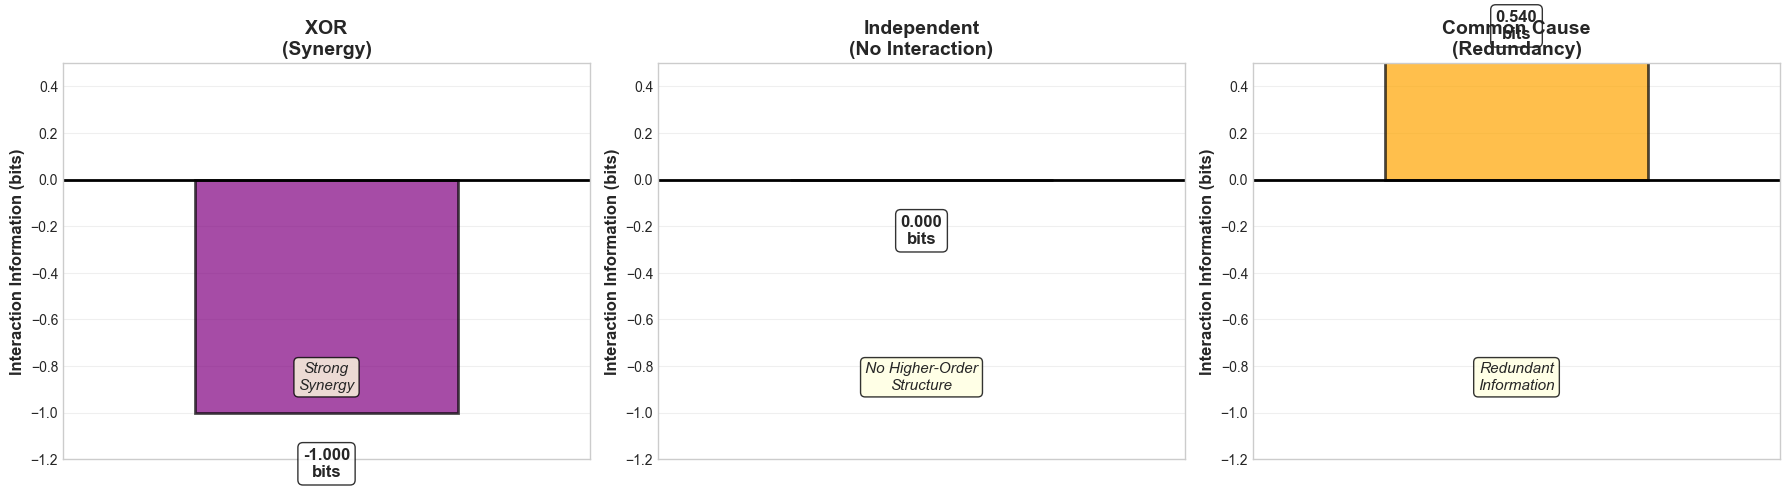
\includegraphics[keepaspectratio]{02_xor_problem_synergy_files/figure-pdf/cell-11-output-1.png}}

\begin{verbatim}

💡 Remember:
  Negative II = Information hidden in combinations (synergy)
  Positive II = Information duplicated across variables (redundancy)
  Zero II = No higher-order interactions
\end{verbatim}

\section{Part 5: The Copy Problem (Pure
Redundancy)}\label{part-5-the-copy-problem-pure-redundancy}

\subsection{The Opposite of XOR}\label{the-opposite-of-xor}

To fully understand synergy, we need to see its opposite: \textbf{pure
redundancy}.

\textbf{Setup}: \(X_2 = X_1\) (perfect copy), and \(Y = X_1\)

Truth table:

\begin{verbatim}
X₁  X₂  │  Y
─────────┼───
0   0   │  0
1   1   │  1
\end{verbatim}

What do you predict will happen here?

\begin{Shaded}
\begin{Highlighting}[]
\CommentTok{\# Create the COPY system}
\NormalTok{P\_COPY }\OperatorTok{=}\NormalTok{ np.zeros((}\DecValTok{2}\NormalTok{, }\DecValTok{2}\NormalTok{, }\DecValTok{2}\NormalTok{))}
\NormalTok{P\_COPY[}\DecValTok{0}\NormalTok{, }\DecValTok{0}\NormalTok{, }\DecValTok{0}\NormalTok{] }\OperatorTok{=} \FloatTok{0.5}  \CommentTok{\# X₁=0, X₂=0, Y=0}
\NormalTok{P\_COPY[}\DecValTok{1}\NormalTok{, }\DecValTok{1}\NormalTok{, }\DecValTok{1}\NormalTok{] }\OperatorTok{=} \FloatTok{0.5}  \CommentTok{\# X₁=1, X₂=1, Y=1}

\CommentTok{\# Calculate all mutual informations}
\NormalTok{P\_X1\_Y\_copy }\OperatorTok{=}\NormalTok{ P\_COPY.}\BuiltInTok{sum}\NormalTok{(axis}\OperatorTok{=}\DecValTok{1}\NormalTok{)}
\NormalTok{P\_X2\_Y\_copy }\OperatorTok{=}\NormalTok{ P\_COPY.}\BuiltInTok{sum}\NormalTok{(axis}\OperatorTok{=}\DecValTok{0}\NormalTok{)}

\NormalTok{MI\_X1\_Y\_copy }\OperatorTok{=}\NormalTok{ mutual\_information(P\_X1\_Y\_copy)}
\NormalTok{MI\_X2\_Y\_copy }\OperatorTok{=}\NormalTok{ mutual\_information(P\_X2\_Y\_copy)}
\NormalTok{MI\_X1X2\_Y\_copy }\OperatorTok{=}\NormalTok{ joint\_mi\_three\_vars(P\_COPY)}
\NormalTok{II\_COPY }\OperatorTok{=}\NormalTok{ interaction\_information(P\_COPY)}

\BuiltInTok{print}\NormalTok{(}\StringTok{"COPY System: X₂ = X₁, Y = X₁"}\NormalTok{)}
\BuiltInTok{print}\NormalTok{(}\StringTok{"="} \OperatorTok{*} \DecValTok{60}\NormalTok{)}
\BuiltInTok{print}\NormalTok{(}\StringTok{"}\CharTok{\textbackslash{}n}\StringTok{Mutual Informations:"}\NormalTok{)}
\BuiltInTok{print}\NormalTok{(}\SpecialStringTok{f"  I(X₁; Y) = }\SpecialCharTok{\{}\NormalTok{MI\_X1\_Y\_copy}\SpecialCharTok{:.4f\}}\SpecialStringTok{ bits"}\NormalTok{)}
\BuiltInTok{print}\NormalTok{(}\SpecialStringTok{f"  I(X₂; Y) = }\SpecialCharTok{\{}\NormalTok{MI\_X2\_Y\_copy}\SpecialCharTok{:.4f\}}\SpecialStringTok{ bits"}\NormalTok{)}
\BuiltInTok{print}\NormalTok{(}\SpecialStringTok{f"  I(X₁, X₂; Y) = }\SpecialCharTok{\{}\NormalTok{MI\_X1X2\_Y\_copy}\SpecialCharTok{:.4f\}}\SpecialStringTok{ bits"}\NormalTok{)}
\BuiltInTok{print}\NormalTok{(}\SpecialStringTok{f"}\CharTok{\textbackslash{}n}\SpecialStringTok{  Interaction Information: }\SpecialCharTok{\{}\NormalTok{II\_COPY}\SpecialCharTok{:.4f\}}\SpecialStringTok{ bits"}\NormalTok{)}

\BuiltInTok{print}\NormalTok{(}\StringTok{"}\CharTok{\textbackslash{}n}\StringTok{"} \OperatorTok{+} \StringTok{"="} \OperatorTok{*} \DecValTok{60}\NormalTok{)}
\BuiltInTok{print}\NormalTok{(}\StringTok{"Interpretation:"}\NormalTok{)}
\BuiltInTok{print}\NormalTok{(}\StringTok{"  {-} Each variable ALONE perfectly predicts Y (1 bit)"}\NormalTok{)}
\BuiltInTok{print}\NormalTok{(}\StringTok{"  {-} Together, they still provide only 1 bit total"}\NormalTok{)}
\BuiltInTok{print}\NormalTok{(}\StringTok{"  {-} The information is REDUNDANT (duplicated)"}\NormalTok{)}
\BuiltInTok{print}\NormalTok{(}\SpecialStringTok{f"  {-} Interaction Info is POSITIVE: }\SpecialCharTok{\{}\NormalTok{II\_COPY}\SpecialCharTok{:.1f\}}\SpecialStringTok{ bit"}\NormalTok{)}
\BuiltInTok{print}\NormalTok{(}\StringTok{"}\CharTok{\textbackslash{}n}\StringTok{  This is the OPPOSITE of XOR!"}\NormalTok{)}
\end{Highlighting}
\end{Shaded}

\begin{verbatim}
COPY System: X₂ = X₁, Y = X₁
============================================================

Mutual Informations:
  I(X₁; Y) = 1.0000 bits
  I(X₂; Y) = 1.0000 bits
  I(X₁, X₂; Y) = 1.0000 bits

  Interaction Information: 2.0000 bits

============================================================
Interpretation:
  - Each variable ALONE perfectly predicts Y (1 bit)
  - Together, they still provide only 1 bit total
  - The information is REDUNDANT (duplicated)
  - Interaction Info is POSITIVE: 2.0 bit

  This is the OPPOSITE of XOR!
\end{verbatim}

\subsection{XOR vs COPY: Side-by-Side
Comparison}\label{xor-vs-copy-side-by-side-comparison}

Let's create a comprehensive comparison to cement these concepts:

\begin{Shaded}
\begin{Highlighting}[]
\CommentTok{\# Create comparison table}
\NormalTok{comparison\_data }\OperatorTok{=}\NormalTok{ \{}
    \StringTok{\textquotesingle{}Measure\textquotesingle{}}\NormalTok{: [}
        \StringTok{\textquotesingle{}I(X₁; Y)\textquotesingle{}}\NormalTok{,}
        \StringTok{\textquotesingle{}I(X₂; Y)\textquotesingle{}}\NormalTok{,}
        \StringTok{\textquotesingle{}I(X₁, X₂; Y)\textquotesingle{}}\NormalTok{,}
        \StringTok{\textquotesingle{}I(X₁; X₂; Y)\textquotesingle{}}\NormalTok{,}
        \StringTok{\textquotesingle{}Type\textquotesingle{}}
\NormalTok{    ],}
    \StringTok{\textquotesingle{}XOR (Synergy)\textquotesingle{}}\NormalTok{: [}
        \SpecialStringTok{f\textquotesingle{}}\SpecialCharTok{\{}\NormalTok{MI\_X1\_Y}\SpecialCharTok{:.1f\}}\SpecialStringTok{\textquotesingle{}}\NormalTok{,}
        \SpecialStringTok{f\textquotesingle{}}\SpecialCharTok{\{}\NormalTok{MI\_X2\_Y}\SpecialCharTok{:.1f\}}\SpecialStringTok{\textquotesingle{}}\NormalTok{,}
        \SpecialStringTok{f\textquotesingle{}}\SpecialCharTok{\{}\NormalTok{MI\_X1X2\_Y}\SpecialCharTok{:.1f\}}\SpecialStringTok{\textquotesingle{}}\NormalTok{,}
        \SpecialStringTok{f\textquotesingle{}}\SpecialCharTok{\{}\NormalTok{II\_XOR}\SpecialCharTok{:.1f\}}\SpecialStringTok{\textquotesingle{}}\NormalTok{,}
        \StringTok{\textquotesingle{}Pure Synergy\textquotesingle{}}
\NormalTok{    ],}
    \StringTok{\textquotesingle{}COPY (Redundancy)\textquotesingle{}}\NormalTok{: [}
        \SpecialStringTok{f\textquotesingle{}}\SpecialCharTok{\{}\NormalTok{MI\_X1\_Y\_copy}\SpecialCharTok{:.1f\}}\SpecialStringTok{\textquotesingle{}}\NormalTok{,}
        \SpecialStringTok{f\textquotesingle{}}\SpecialCharTok{\{}\NormalTok{MI\_X2\_Y\_copy}\SpecialCharTok{:.1f\}}\SpecialStringTok{\textquotesingle{}}\NormalTok{,}
        \SpecialStringTok{f\textquotesingle{}}\SpecialCharTok{\{}\NormalTok{MI\_X1X2\_Y\_copy}\SpecialCharTok{:.1f\}}\SpecialStringTok{\textquotesingle{}}\NormalTok{,}
        \SpecialStringTok{f\textquotesingle{}}\SpecialCharTok{\{}\NormalTok{II\_COPY}\SpecialCharTok{:.1f\}}\SpecialStringTok{\textquotesingle{}}\NormalTok{,}
        \StringTok{\textquotesingle{}Pure Redundancy\textquotesingle{}}
\NormalTok{    ]}
\NormalTok{\}}

\NormalTok{df }\OperatorTok{=}\NormalTok{ pd.DataFrame(comparison\_data)}
\BuiltInTok{print}\NormalTok{(}\StringTok{"}\CharTok{\textbackslash{}n}\StringTok{XOR vs COPY: The Two Extremes"}\NormalTok{)}
\BuiltInTok{print}\NormalTok{(}\StringTok{"="} \OperatorTok{*} \DecValTok{70}\NormalTok{)}
\BuiltInTok{print}\NormalTok{(df.to\_string(index}\OperatorTok{=}\VariableTok{False}\NormalTok{))}
\BuiltInTok{print}\NormalTok{(}\StringTok{"="} \OperatorTok{*} \DecValTok{70}\NormalTok{)}

\BuiltInTok{print}\NormalTok{(}\StringTok{"}\CharTok{\textbackslash{}n}\StringTok{🎯 KEY INSIGHTS:"}\NormalTok{)}
\BuiltInTok{print}\NormalTok{(}\StringTok{"}\CharTok{\textbackslash{}n}\StringTok{SYNERGY (XOR):"}\NormalTok{)}
\BuiltInTok{print}\NormalTok{(}\StringTok{"  • Individual variables: Useless (0 bits)"}\NormalTok{)}
\BuiltInTok{print}\NormalTok{(}\StringTok{"  • Combined: Perfect prediction (1 bit)"}\NormalTok{)}
\BuiltInTok{print}\NormalTok{(}\StringTok{"  • Information \textquotesingle{}emerges\textquotesingle{} from combination"}\NormalTok{)}
\BuiltInTok{print}\NormalTok{(}\StringTok{"  • Interaction information: NEGATIVE"}\NormalTok{)}

\BuiltInTok{print}\NormalTok{(}\StringTok{"}\CharTok{\textbackslash{}n}\StringTok{REDUNDANCY (COPY):"}\NormalTok{)}
\BuiltInTok{print}\NormalTok{(}\StringTok{"  • Individual variables: Perfect (1 bit each)"}\NormalTok{)}
\BuiltInTok{print}\NormalTok{(}\StringTok{"  • Combined: No additional info (still 1 bit)"}\NormalTok{)}
\BuiltInTok{print}\NormalTok{(}\StringTok{"  • Information \textquotesingle{}duplicated\textquotesingle{} across variables"}\NormalTok{)}
\BuiltInTok{print}\NormalTok{(}\StringTok{"  • Interaction information: POSITIVE"}\NormalTok{)}

\BuiltInTok{print}\NormalTok{(}\StringTok{"}\CharTok{\textbackslash{}n}\StringTok{"} \OperatorTok{+} \StringTok{"="} \OperatorTok{*} \DecValTok{70}\NormalTok{)}
\BuiltInTok{print}\NormalTok{(}\StringTok{"Real systems typically have MIXTURES of both synergy and redundancy!"}\NormalTok{)}
\BuiltInTok{print}\NormalTok{(}\StringTok{"That\textquotesingle{}s what Partial Information Decomposition (PID) quantifies."}\NormalTok{)}
\BuiltInTok{print}\NormalTok{(}\StringTok{"We\textquotesingle{}ll explore PID in Notebook 3 using the HOI package!"}\NormalTok{)}
\end{Highlighting}
\end{Shaded}

\begin{verbatim}

XOR vs COPY: The Two Extremes
======================================================================
     Measure XOR (Synergy) COPY (Redundancy)
    I(X₁; Y)           0.0               1.0
    I(X₂; Y)           0.0               1.0
I(X₁, X₂; Y)           1.0               1.0
I(X₁; X₂; Y)          -1.0               2.0
        Type  Pure Synergy   Pure Redundancy
======================================================================

🎯 KEY INSIGHTS:

SYNERGY (XOR):
  • Individual variables: Useless (0 bits)
  • Combined: Perfect prediction (1 bit)
  • Information 'emerges' from combination
  • Interaction information: NEGATIVE

REDUNDANCY (COPY):
  • Individual variables: Perfect (1 bit each)
  • Combined: No additional info (still 1 bit)
  • Information 'duplicated' across variables
  • Interaction information: POSITIVE

======================================================================
Real systems typically have MIXTURES of both synergy and redundancy!
That's what Partial Information Decomposition (PID) quantifies.
We'll explore PID in Notebook 3 using the HOI package!
\end{verbatim}

\section{Part 6: The Explaining Away
Effect}\label{part-6-the-explaining-away-effect}

\subsection{When Conditioning Increases
Dependence}\label{when-conditioning-increases-dependence}

We mentioned earlier that conditioning can \textbf{increase} mutual
information. This phenomenon, called ``explaining away,'' is crucial for
understanding conditional independence.

\subsection{The Classic Example: Alarm
System}\label{the-classic-example-alarm-system}

Imagine: - \(X_1\) = Earthquake (0 = no, 1 = yes) - \(X_2\) = Burglary
(0 = no, 1 = yes)\\
- \(Y\) = Alarm rings (0 = silent, 1 = ringing)

\textbf{Without knowing if alarm rang}: Earthquakes and burglaries are
independent events.

\textbf{After hearing alarm}: If you learn there was an earthquake, that
\textbf{explains away} the alarm, making burglary less likely!

Therefore: \(I(X_1; X_2) = 0\) but \(I(X_1; X_2 | Y) > 0\)

This means \(I(X_1; X_2; Y) > 0\) (positive interaction information =
redundancy).

\begin{Shaded}
\begin{Highlighting}[]
\CommentTok{\# Create alarm system distribution}
\NormalTok{P\_alarm }\OperatorTok{=}\NormalTok{ np.zeros((}\DecValTok{2}\NormalTok{, }\DecValTok{2}\NormalTok{, }\DecValTok{2}\NormalTok{))  }\CommentTok{\# (Earthquake, Burglary, Alarm)}

\CommentTok{\# Prior probabilities (very low)}
\NormalTok{p\_earthquake }\OperatorTok{=} \FloatTok{0.01}
\NormalTok{p\_burglary }\OperatorTok{=} \FloatTok{0.02}

\CommentTok{\# Alarm probabilities}
\NormalTok{p\_alarm\_both }\OperatorTok{=} \FloatTok{0.99}  \CommentTok{\# If both → almost certainly rings}
\NormalTok{p\_alarm\_quake }\OperatorTok{=} \FloatTok{0.90}  \CommentTok{\# If earthquake alone}
\NormalTok{p\_alarm\_burg }\OperatorTok{=} \FloatTok{0.85}   \CommentTok{\# If burglary alone}
\NormalTok{p\_alarm\_neither }\OperatorTok{=} \FloatTok{0.01}  \CommentTok{\# False alarm rate}

\CommentTok{\# Fill in the joint distribution}
\CommentTok{\# No earthquake, no burglary}
\NormalTok{P\_alarm[}\DecValTok{0}\NormalTok{, }\DecValTok{0}\NormalTok{, }\DecValTok{0}\NormalTok{] }\OperatorTok{=}\NormalTok{ (}\DecValTok{1} \OperatorTok{{-}}\NormalTok{ p\_earthquake) }\OperatorTok{*}\NormalTok{ (}\DecValTok{1} \OperatorTok{{-}}\NormalTok{ p\_burglary) }\OperatorTok{*}\NormalTok{ (}\DecValTok{1} \OperatorTok{{-}}\NormalTok{ p\_alarm\_neither)}
\NormalTok{P\_alarm[}\DecValTok{0}\NormalTok{, }\DecValTok{0}\NormalTok{, }\DecValTok{1}\NormalTok{] }\OperatorTok{=}\NormalTok{ (}\DecValTok{1} \OperatorTok{{-}}\NormalTok{ p\_earthquake) }\OperatorTok{*}\NormalTok{ (}\DecValTok{1} \OperatorTok{{-}}\NormalTok{ p\_burglary) }\OperatorTok{*}\NormalTok{ p\_alarm\_neither}

\CommentTok{\# Earthquake, no burglary}
\NormalTok{P\_alarm[}\DecValTok{1}\NormalTok{, }\DecValTok{0}\NormalTok{, }\DecValTok{0}\NormalTok{] }\OperatorTok{=}\NormalTok{ p\_earthquake }\OperatorTok{*}\NormalTok{ (}\DecValTok{1} \OperatorTok{{-}}\NormalTok{ p\_burglary) }\OperatorTok{*}\NormalTok{ (}\DecValTok{1} \OperatorTok{{-}}\NormalTok{ p\_alarm\_quake)}
\NormalTok{P\_alarm[}\DecValTok{1}\NormalTok{, }\DecValTok{0}\NormalTok{, }\DecValTok{1}\NormalTok{] }\OperatorTok{=}\NormalTok{ p\_earthquake }\OperatorTok{*}\NormalTok{ (}\DecValTok{1} \OperatorTok{{-}}\NormalTok{ p\_burglary) }\OperatorTok{*}\NormalTok{ p\_alarm\_quake}

\CommentTok{\# No earthquake, burglary}
\NormalTok{P\_alarm[}\DecValTok{0}\NormalTok{, }\DecValTok{1}\NormalTok{, }\DecValTok{0}\NormalTok{] }\OperatorTok{=}\NormalTok{ (}\DecValTok{1} \OperatorTok{{-}}\NormalTok{ p\_earthquake) }\OperatorTok{*}\NormalTok{ p\_burglary }\OperatorTok{*}\NormalTok{ (}\DecValTok{1} \OperatorTok{{-}}\NormalTok{ p\_alarm\_burg)}
\NormalTok{P\_alarm[}\DecValTok{0}\NormalTok{, }\DecValTok{1}\NormalTok{, }\DecValTok{1}\NormalTok{] }\OperatorTok{=}\NormalTok{ (}\DecValTok{1} \OperatorTok{{-}}\NormalTok{ p\_earthquake) }\OperatorTok{*}\NormalTok{ p\_burglary }\OperatorTok{*}\NormalTok{ p\_alarm\_burg}

\CommentTok{\# Both}
\NormalTok{P\_alarm[}\DecValTok{1}\NormalTok{, }\DecValTok{1}\NormalTok{, }\DecValTok{0}\NormalTok{] }\OperatorTok{=}\NormalTok{ p\_earthquake }\OperatorTok{*}\NormalTok{ p\_burglary }\OperatorTok{*}\NormalTok{ (}\DecValTok{1} \OperatorTok{{-}}\NormalTok{ p\_alarm\_both)}
\NormalTok{P\_alarm[}\DecValTok{1}\NormalTok{, }\DecValTok{1}\NormalTok{, }\DecValTok{1}\NormalTok{] }\OperatorTok{=}\NormalTok{ p\_earthquake }\OperatorTok{*}\NormalTok{ p\_burglary }\OperatorTok{*}\NormalTok{ p\_alarm\_both}

\CommentTok{\# Calculate unconditional MI}
\NormalTok{P\_E\_B }\OperatorTok{=}\NormalTok{ P\_alarm.}\BuiltInTok{sum}\NormalTok{(axis}\OperatorTok{=}\DecValTok{2}\NormalTok{)  }\CommentTok{\# Marginalize alarm}
\NormalTok{MI\_E\_B }\OperatorTok{=}\NormalTok{ mutual\_information(P\_E\_B)}

\CommentTok{\# Calculate conditional MI given alarm = 1}
\CommentTok{\# P(E, B | Alarm=1)}
\NormalTok{P\_alarm\_1 }\OperatorTok{=}\NormalTok{ P\_alarm[:, :, }\DecValTok{1}\NormalTok{].}\BuiltInTok{sum}\NormalTok{()}
\ControlFlowTok{if}\NormalTok{ P\_alarm\_1 }\OperatorTok{\textgreater{}} \DecValTok{0}\NormalTok{:}
\NormalTok{    P\_E\_B\_given\_alarm }\OperatorTok{=}\NormalTok{ P\_alarm[:, :, }\DecValTok{1}\NormalTok{] }\OperatorTok{/}\NormalTok{ P\_alarm\_1}
\NormalTok{    MI\_E\_B\_given\_alarm }\OperatorTok{=}\NormalTok{ mutual\_information(P\_E\_B\_given\_alarm)}
\ControlFlowTok{else}\NormalTok{:}
\NormalTok{    MI\_E\_B\_given\_alarm }\OperatorTok{=} \DecValTok{0}

\BuiltInTok{print}\NormalTok{(}\StringTok{"Explaining Away: The Alarm System"}\NormalTok{)}
\BuiltInTok{print}\NormalTok{(}\StringTok{"="} \OperatorTok{*} \DecValTok{60}\NormalTok{)}
\BuiltInTok{print}\NormalTok{(}\StringTok{"}\CharTok{\textbackslash{}n}\StringTok{Scenario: Earthquake and Burglary both trigger alarm"}\NormalTok{)}
\BuiltInTok{print}\NormalTok{(}\StringTok{"}\CharTok{\textbackslash{}n}\StringTok{Mutual Information:"}\NormalTok{)}
\BuiltInTok{print}\NormalTok{(}\SpecialStringTok{f"  I(Earthquake; Burglary) = }\SpecialCharTok{\{}\NormalTok{MI\_E\_B}\SpecialCharTok{:.6f\}}\SpecialStringTok{ bits"}\NormalTok{)}
\BuiltInTok{print}\NormalTok{(}\SpecialStringTok{f"  I(Earthquake; Burglary | Alarm=1) = }\SpecialCharTok{\{}\NormalTok{MI\_E\_B\_given\_alarm}\SpecialCharTok{:.4f\}}\SpecialStringTok{ bits"}\NormalTok{)}

\ControlFlowTok{if}\NormalTok{ MI\_E\_B\_given\_alarm }\OperatorTok{\textgreater{}}\NormalTok{ MI\_E\_B:}
\NormalTok{    increase }\OperatorTok{=}\NormalTok{ MI\_E\_B\_given\_alarm }\OperatorTok{{-}}\NormalTok{ MI\_E\_B}
    \BuiltInTok{print}\NormalTok{(}\SpecialStringTok{f"}\CharTok{\textbackslash{}n}\SpecialStringTok{  ⬆️  Conditioning INCREASED MI by }\SpecialCharTok{\{}\NormalTok{increase}\SpecialCharTok{:.4f\}}\SpecialStringTok{ bits!"}\NormalTok{)}
    \BuiltInTok{print}\NormalTok{(}\StringTok{"}\CharTok{\textbackslash{}n}\StringTok{Interpretation:"}\NormalTok{)}
    \BuiltInTok{print}\NormalTok{(}\StringTok{"  • Before knowing alarm status: Events are independent"}\NormalTok{)}
    \BuiltInTok{print}\NormalTok{(}\StringTok{"  • After hearing alarm: They become dependent!"}\NormalTok{)}
    \BuiltInTok{print}\NormalTok{(}\StringTok{"  • Learning \textquotesingle{}earthquake\textquotesingle{} explains away \textquotesingle{}burglary\textquotesingle{} hypothesis"}\NormalTok{)}
    \BuiltInTok{print}\NormalTok{(}\StringTok{"}\CharTok{\textbackslash{}n}\StringTok{  This violates our Venn diagram intuition!"}\NormalTok{)}

\BuiltInTok{print}\NormalTok{(}\StringTok{"}\CharTok{\textbackslash{}n}\StringTok{"} \OperatorTok{+} \StringTok{"="} \OperatorTok{*} \DecValTok{60}\NormalTok{)}
\BuiltInTok{print}\NormalTok{(}\StringTok{"This is why we need multivariate measures!"}\NormalTok{)}
\BuiltInTok{print}\NormalTok{(}\StringTok{"Pairwise MI alone misses these higher{-}order dependencies."}\NormalTok{)}
\end{Highlighting}
\end{Shaded}

\begin{verbatim}
Explaining Away: The Alarm System
============================================================

Scenario: Earthquake and Burglary both trigger alarm

Mutual Information:
  I(Earthquake; Burglary) = -0.000000 bits
  I(Earthquake; Burglary | Alarm=1) = 0.2531 bits

  ⬆️  Conditioning INCREASED MI by 0.2531 bits!

Interpretation:
  • Before knowing alarm status: Events are independent
  • After hearing alarm: They become dependent!
  • Learning 'earthquake' explains away 'burglary' hypothesis

  This violates our Venn diagram intuition!

============================================================
This is why we need multivariate measures!
Pairwise MI alone misses these higher-order dependencies.
\end{verbatim}

\section{Summary and Next Steps}\label{summary-and-next-steps}

\subsection{What We've Discovered}\label{what-weve-discovered}

Congratulations! You've just experienced one of the most important
``aha!'' moments in information theory:

\begin{enumerate}
\def\labelenumi{\arabic{enumi}.}
\tightlist
\item
  \textbf{XOR Problem}: Two variables can individually carry zero
  information yet together carry maximal information
\item
  \textbf{Venn Diagrams Fail}: The classic visualization breaks down for
  3+ variables
\item
  \textbf{Interaction Information}: A signed measure that can be
  negative (synergy) or positive (redundancy)
\item
  \textbf{Pure Synergy vs Pure Redundancy}: XOR and COPY represent two
  extremes
\item
  \textbf{Explaining Away}: Conditioning can increase mutual information
\end{enumerate}

\subsection{The Deep Insight}\label{the-deep-insight}

\textbf{Information is not additive} in multivariate systems. The whole
can be: - \textbf{More} than the sum of its parts (synergy) -
\textbf{Less} than the sum of its parts (redundancy) - \textbf{Equal to}
the sum of its parts (independence)

\subsection{Why This Matters for
Neuroscience}\label{why-this-matters-for-neuroscience}

Neural systems exhibit both synergy and redundancy: -
\textbf{Synergistic coding}: Population provides more information than
sum of individuals - \textbf{Redundant coding}: Multiple neurons encode
the same information (robustness) - \textbf{Real populations}: Mixture
of both!

\subsection{Coming Up in Notebook 3}\label{coming-up-in-notebook-3}

We'll use the \textbf{HOI (Higher-Order Interactions) package} to: -
Calculate O-information and S-information - Decompose information using
Partial Information Decomposition (PID) - Quantify the four ``atoms'':
Unique(X₁), Unique(X₂), Redundancy, Synergy - Apply these to simulated
neural data - Understand when to use each measure

\subsection{Practice Problems}\label{practice-problems}

\begin{Shaded}
\begin{Highlighting}[]
\BuiltInTok{print}\NormalTok{(}\StringTok{"PRACTICE EXERCISES"}\NormalTok{)}
\BuiltInTok{print}\NormalTok{(}\StringTok{"="} \OperatorTok{*} \DecValTok{70}\NormalTok{)}

\BuiltInTok{print}\NormalTok{(}\StringTok{"}\CharTok{\textbackslash{}n}\StringTok{1. Create an AND gate: Y = X₁ AND X₂"}\NormalTok{)}
\BuiltInTok{print}\NormalTok{(}\StringTok{"   Calculate I(X₁; Y), I(X₂; Y), and I(X₁,X₂; Y)"}\NormalTok{)}
\BuiltInTok{print}\NormalTok{(}\StringTok{"   Is interaction information positive or negative?"}\NormalTok{)}
\BuiltInTok{print}\NormalTok{(}\StringTok{"   Hint: AND is partially redundant {-} one input can sometimes predict output"}\NormalTok{)}

\BuiltInTok{print}\NormalTok{(}\StringTok{"}\CharTok{\textbackslash{}n}\StringTok{2. What happens if you have 3 variables in XOR: Y = X₁ XOR X₂ XOR X₃?"}\NormalTok{)}
\BuiltInTok{print}\NormalTok{(}\StringTok{"   Predict: Will synergy be even stronger?"}\NormalTok{)}

\BuiltInTok{print}\NormalTok{(}\StringTok{"}\CharTok{\textbackslash{}n}\StringTok{3. Design a system with EXACTLY zero interaction information."}\NormalTok{)}
\BuiltInTok{print}\NormalTok{(}\StringTok{"   Hint: What if the three variables are mutually independent?"}\NormalTok{)}

\BuiltInTok{print}\NormalTok{(}\StringTok{"}\CharTok{\textbackslash{}n}\StringTok{4. In the alarm example, calculate P(Earthquake | Alarm=1, Burglary=0)."}\NormalTok{)}
\BuiltInTok{print}\NormalTok{(}\StringTok{"   How does this compare to P(Earthquake)?"}\NormalTok{)}
\BuiltInTok{print}\NormalTok{(}\StringTok{"   This is Bayesian reasoning using information theory!"}\NormalTok{)}

\BuiltInTok{print}\NormalTok{(}\StringTok{"}\CharTok{\textbackslash{}n}\StringTok{"} \OperatorTok{+} \StringTok{"="} \OperatorTok{*} \DecValTok{70}\NormalTok{)}
\BuiltInTok{print}\NormalTok{(}\StringTok{"}\CharTok{\textbackslash{}n}\StringTok{Ready for Notebook 3: Higher{-}Order Interactions with HOI!"}\NormalTok{)}
\BuiltInTok{print}\NormalTok{(}\StringTok{"There we\textquotesingle{}ll use a professional package to compute all these measures"}\NormalTok{)}
\BuiltInTok{print}\NormalTok{(}\StringTok{"and apply them to realistic neural data scenarios."}\NormalTok{)}
\BuiltInTok{print}\NormalTok{(}\StringTok{"="} \OperatorTok{*} \DecValTok{70}\NormalTok{)}
\end{Highlighting}
\end{Shaded}

\begin{verbatim}
PRACTICE EXERCISES
======================================================================

1. Create an AND gate: Y = X₁ AND X₂
   Calculate I(X₁; Y), I(X₂; Y), and I(X₁,X₂; Y)
   Is interaction information positive or negative?
   Hint: AND is partially redundant - one input can sometimes predict output

2. What happens if you have 3 variables in XOR: Y = X₁ XOR X₂ XOR X₃?
   Predict: Will synergy be even stronger?

3. Design a system with EXACTLY zero interaction information.
   Hint: What if the three variables are mutually independent?

4. In the alarm example, calculate P(Earthquake | Alarm=1, Burglary=0).
   How does this compare to P(Earthquake)?
   This is Bayesian reasoning using information theory!

======================================================================

Ready for Notebook 3: Higher-Order Interactions with HOI!
There we'll use a professional package to compute all these measures
and apply them to realistic neural data scenarios.
======================================================================
\end{verbatim}

\section{Further Reading}\label{further-reading}

\subsection{Essential Papers}\label{essential-papers}

\begin{enumerate}
\def\labelenumi{\arabic{enumi}.}
\tightlist
\item
  \textbf{Williams \& Beer (2010)} - ``Nonnegative Decomposition of
  Multivariate Information''

  \begin{itemize}
  \tightlist
  \item
    Original PID framework
  \item
    Defines the four information atoms
  \end{itemize}
\item
  \textbf{Schneidman et al.~(2003)} - ``Synergy, redundancy, and
  independence in population codes''

  \begin{itemize}
  \tightlist
  \item
    Neural applications of synergy
  \item
    Blowfly H1 neuron example
  \end{itemize}
\item
  \textbf{Timme \& Lapish (2018)} - ``A tutorial for information theory
  in neuroscience''

  \begin{itemize}
  \tightlist
  \item
    Excellent pedagogical resource
  \item
    Practical examples
  \end{itemize}
\end{enumerate}

\subsection{Advanced Topics}\label{advanced-topics}

\begin{itemize}
\tightlist
\item
  \textbf{O-information}: Extends interaction information to N variables
\item
  \textbf{Integrated Information Theory (IIT)}: Uses synergy concepts
  for consciousness
\item
  \textbf{Transfer Entropy}: Directed information flow
\item
  \textbf{Granger Causality}: Statistical causation (related to transfer
  entropy)
\end{itemize}

See you in Notebook 3! 🚀

\part{Part II: Advanced Tools}

\chapter{Notebook 3: Higher-Order Interactions with
HOI}\label{notebook-3-higher-order-interactions-with-hoi}

\section{From Manual Calculations to Professional
Tools}\label{from-manual-calculations-to-professional-tools}

Welcome to the third notebook in our series! In Notebooks 1 and 2, you
built a deep understanding of information theory and discovered the
shocking XOR result. You calculated everything by hand, which gave you
crucial intuition about how these measures work.

Now it's time to scale up. Computing interaction information for even
modest systems (say, 20 neurons with all possible triplets) means
thousands of calculations. Doing this by hand would take forever and be
error-prone. This is where the \textbf{HOI (Higher-Order Interactions)}
package comes in.

\subsection{What is HOI?}\label{what-is-hoi}

HOI is a Python package specifically designed for computing higher-order
information-theoretic measures. Built on top of JAX (which allows
computation on GPUs), it provides: - \textbf{O-information}: Detects
synergy vs redundancy - \textbf{S-information}: Measures total
complexity - \textbf{Partial Information Decomposition (PID)}:
Decomposes information into atoms - \textbf{Multiple estimators}:
Gaussian copula, KNN, binning, and more - \textbf{Efficient
computation}: Handles large datasets

\subsection{Why This Matters for Your
Research}\label{why-this-matters-for-your-research}

HOI bridges the gap between theory and application. You can: - Analyze
real neural recordings - Discover synergistic ensembles automatically -
Quantify redundancy in population codes - Test hypotheses about
information structure

\subsection{Learning Objectives}\label{learning-objectives-1}

By the end of this notebook, you'll: 1. Install and configure HOI 2.
Compute O-information and interpret its sign 3. Use Partial Information
Decomposition (PID) 4. Apply multiple estimators and understand their
trade-offs 5. Analyze simulated neural population data 6. Understand
computational scaling and optimization strategies 7. Know when to use
each measure

Let's dive in! 🚀

\section{Part 1: Installation and
Setup}\label{part-1-installation-and-setup}

\subsection{Installing HOI}\label{installing-hoi}

HOI requires JAX, which provides fast numerical computation and can use
GPUs if available. We'll install both packages together.

\textbf{Important Note}: JAX installation varies by system. The default
installation works for CPU-only computation. If you have a GPU and want
to use it, consult the
\href{https://github.com/google/jax\#installation}{JAX installation
guide}.

For most users, the simple CPU version is sufficient for learning and
moderate-scale analyses.

\begin{Shaded}
\begin{Highlighting}[]
\CommentTok{\# Install HOI and its dependencies}
\CommentTok{\# This may take a minute or two}
\OperatorTok{!}\NormalTok{pip install }\OperatorTok{{-}}\NormalTok{q hoi jax jaxlib numpy scipy matplotlib seaborn pandas scikit}\OperatorTok{{-}}\NormalTok{learn}

\BuiltInTok{print}\NormalTok{(}\StringTok{"Installation complete!"}\NormalTok{)}
\BuiltInTok{print}\NormalTok{(}\StringTok{"Let\textquotesingle{}s verify everything works..."}\NormalTok{)}
\end{Highlighting}
\end{Shaded}

\begin{verbatim}
Installation complete!
Let's verify everything works...
\end{verbatim}

\begin{Shaded}
\begin{Highlighting}[]
\CommentTok{\# Import all necessary libraries}
\ImportTok{import}\NormalTok{ numpy }\ImportTok{as}\NormalTok{ np}
\ImportTok{import}\NormalTok{ matplotlib.pyplot }\ImportTok{as}\NormalTok{ plt}
\ImportTok{import}\NormalTok{ seaborn }\ImportTok{as}\NormalTok{ sns}
\ImportTok{from}\NormalTok{ scipy }\ImportTok{import}\NormalTok{ stats}
\ImportTok{import}\NormalTok{ pandas }\ImportTok{as}\NormalTok{ pd}
\ImportTok{from}\NormalTok{ itertools }\ImportTok{import}\NormalTok{ combinations, product}
\ImportTok{import}\NormalTok{ warnings}
\NormalTok{warnings.filterwarnings(}\StringTok{\textquotesingle{}ignore\textquotesingle{}}\NormalTok{)}

\CommentTok{\# Import HOI modules}
\ImportTok{import}\NormalTok{ hoi}
\ImportTok{from}\NormalTok{ hoi.metrics }\ImportTok{import}\NormalTok{ Oinfo, InfoTopo, TC, DTC, Sinfo}
\ImportTok{from}\NormalTok{ hoi.metrics }\ImportTok{import}\NormalTok{ RedundancyMMI, SynergyMMI  }\CommentTok{\# PID measures}
\ImportTok{from}\NormalTok{ hoi.core }\ImportTok{import}\NormalTok{ get\_entropy, get\_mi}
\ImportTok{from}\NormalTok{ hoi.utils }\ImportTok{import}\NormalTok{ get\_nbest\_mult}

\CommentTok{\# Set random seed for reproducibility}
\NormalTok{np.random.seed(}\DecValTok{42}\NormalTok{)}

\CommentTok{\# Configure plotting}
\NormalTok{plt.style.use(}\StringTok{\textquotesingle{}seaborn{-}v0\_8{-}whitegrid\textquotesingle{}}\NormalTok{)}
\NormalTok{sns.set\_palette(}\StringTok{"husl"}\NormalTok{)}
\OperatorTok{\%}\NormalTok{matplotlib inline}

\BuiltInTok{print}\NormalTok{(}\SpecialStringTok{f"HOI version: }\SpecialCharTok{\{}\NormalTok{hoi}\SpecialCharTok{.}\NormalTok{\_\_version\_\_}\SpecialCharTok{\}}\SpecialStringTok{"}\NormalTok{)}
\BuiltInTok{print}\NormalTok{(}\StringTok{"All libraries loaded successfully!"}\NormalTok{)}
\BuiltInTok{print}\NormalTok{(}\StringTok{"}\CharTok{\textbackslash{}n}\StringTok{🎉 Ready to explore higher{-}order interactions!"}\NormalTok{)}
\end{Highlighting}
\end{Shaded}

\begin{verbatim}
HOI version: 0.0.5
All libraries loaded successfully!

🎉 Ready to explore higher-order interactions!
\end{verbatim}

\subsection{Understanding HOI's Data
Format}\label{understanding-hois-data-format}

Before we start computing, we need to understand how HOI expects data to
be organized. This is crucial because getting the format wrong is the
\#1 source of errors.

\textbf{HOI Data Convention}:

\begin{verbatim}
data.shape = (n_samples, n_features)
\end{verbatim}

This means: - \textbf{Rows}: Different observations (time points,
trials, subjects, etc.) - \textbf{Columns}: Different variables
(neurons, sensors, brain regions, etc.)

\textbf{Important}: This matches scikit-learn convention: (n\_samples,
n\_features). Each row is one observation of all variables.

Let's create some example data to verify we understand:

\begin{Shaded}
\begin{Highlighting}[]
\CommentTok{\# Create simple test data}
\NormalTok{n\_neurons }\OperatorTok{=} \DecValTok{5}
\NormalTok{n\_trials }\OperatorTok{=} \DecValTok{1000}

\CommentTok{\# Generate random data in HOI format: (n\_samples, n\_features)}
\NormalTok{test\_data }\OperatorTok{=}\NormalTok{ np.random.randn(n\_trials, n\_neurons)}

\BuiltInTok{print}\NormalTok{(}\StringTok{"Test Data Shape Check"}\NormalTok{)}
\BuiltInTok{print}\NormalTok{(}\StringTok{"="} \OperatorTok{*} \DecValTok{50}\NormalTok{)}
\BuiltInTok{print}\NormalTok{(}\SpecialStringTok{f"Data shape: }\SpecialCharTok{\{}\NormalTok{test\_data}\SpecialCharTok{.}\NormalTok{shape}\SpecialCharTok{\}}\SpecialStringTok{"}\NormalTok{)}
\BuiltInTok{print}\NormalTok{(}\SpecialStringTok{f"  {-} First dimension (}\SpecialCharTok{\{}\NormalTok{test\_data}\SpecialCharTok{.}\NormalTok{shape[}\DecValTok{0}\NormalTok{]}\SpecialCharTok{\}}\SpecialStringTok{): Number of trials/samples"}\NormalTok{)}
\BuiltInTok{print}\NormalTok{(}\SpecialStringTok{f"  {-} Second dimension (}\SpecialCharTok{\{}\NormalTok{test\_data}\SpecialCharTok{.}\NormalTok{shape[}\DecValTok{1}\NormalTok{]}\SpecialCharTok{\}}\SpecialStringTok{): Number of neurons/features"}\NormalTok{)}
\BuiltInTok{print}\NormalTok{(}\StringTok{"}\CharTok{\textbackslash{}n}\StringTok{✓ Correct format: (n\_samples, n\_features)"}\NormalTok{)}
\BuiltInTok{print}\NormalTok{(}\StringTok{"}\CharTok{\textbackslash{}n}\StringTok{Each row is a snapshot of all neurons at one trial"}\NormalTok{)}
\BuiltInTok{print}\NormalTok{(}\StringTok{"Each column is a neuron\textquotesingle{}s activity across all trials"}\NormalTok{)}

\CommentTok{\# Visualize what this means}
\NormalTok{fig, axes }\OperatorTok{=}\NormalTok{ plt.subplots(}\DecValTok{1}\NormalTok{, }\DecValTok{2}\NormalTok{, figsize}\OperatorTok{=}\NormalTok{(}\DecValTok{14}\NormalTok{, }\DecValTok{5}\NormalTok{))}

\CommentTok{\# Plot 1: Activity of first neuron across trials (one column)}
\NormalTok{ax1 }\OperatorTok{=}\NormalTok{ axes[}\DecValTok{0}\NormalTok{]}
\NormalTok{ax1.plot(test\_data[:}\DecValTok{200}\NormalTok{, }\DecValTok{0}\NormalTok{], linewidth}\OperatorTok{=}\FloatTok{1.5}\NormalTok{, color}\OperatorTok{=}\StringTok{\textquotesingle{}\#E63946\textquotesingle{}}\NormalTok{)}
\NormalTok{ax1.set\_xlabel(}\StringTok{\textquotesingle{}Trial Number\textquotesingle{}}\NormalTok{, fontsize}\OperatorTok{=}\DecValTok{12}\NormalTok{, fontweight}\OperatorTok{=}\StringTok{\textquotesingle{}bold\textquotesingle{}}\NormalTok{)}
\NormalTok{ax1.set\_ylabel(}\StringTok{\textquotesingle{}Activity\textquotesingle{}}\NormalTok{, fontsize}\OperatorTok{=}\DecValTok{12}\NormalTok{, fontweight}\OperatorTok{=}\StringTok{\textquotesingle{}bold\textquotesingle{}}\NormalTok{)}
\NormalTok{ax1.set\_title(}\StringTok{\textquotesingle{}Single Neuron Across Trials}\CharTok{\textbackslash{}n}\StringTok{(One column of data matrix)\textquotesingle{}}\NormalTok{, }
\NormalTok{              fontsize}\OperatorTok{=}\DecValTok{13}\NormalTok{, fontweight}\OperatorTok{=}\StringTok{\textquotesingle{}bold\textquotesingle{}}\NormalTok{)}
\NormalTok{ax1.grid(}\VariableTok{True}\NormalTok{, alpha}\OperatorTok{=}\FloatTok{0.3}\NormalTok{)}

\CommentTok{\# Plot 2: Snapshot of all neurons at one trial (one row)}
\NormalTok{ax2 }\OperatorTok{=}\NormalTok{ axes[}\DecValTok{1}\NormalTok{]}
\NormalTok{trial\_snapshot }\OperatorTok{=}\NormalTok{ test\_data[}\DecValTok{0}\NormalTok{, :]}
\NormalTok{ax2.bar(}\BuiltInTok{range}\NormalTok{(n\_neurons), trial\_snapshot, color}\OperatorTok{=}\StringTok{\textquotesingle{}\#457B9D\textquotesingle{}}\NormalTok{, alpha}\OperatorTok{=}\FloatTok{0.7}\NormalTok{, edgecolor}\OperatorTok{=}\StringTok{\textquotesingle{}black\textquotesingle{}}\NormalTok{)}
\NormalTok{ax2.set\_xlabel(}\StringTok{\textquotesingle{}Neuron ID\textquotesingle{}}\NormalTok{, fontsize}\OperatorTok{=}\DecValTok{12}\NormalTok{, fontweight}\OperatorTok{=}\StringTok{\textquotesingle{}bold\textquotesingle{}}\NormalTok{)}
\NormalTok{ax2.set\_ylabel(}\StringTok{\textquotesingle{}Activity\textquotesingle{}}\NormalTok{, fontsize}\OperatorTok{=}\DecValTok{12}\NormalTok{, fontweight}\OperatorTok{=}\StringTok{\textquotesingle{}bold\textquotesingle{}}\NormalTok{)}
\NormalTok{ax2.set\_title(}\StringTok{\textquotesingle{}All Neurons at One Trial}\CharTok{\textbackslash{}n}\StringTok{(One row of data matrix)\textquotesingle{}}\NormalTok{, }
\NormalTok{              fontsize}\OperatorTok{=}\DecValTok{13}\NormalTok{, fontweight}\OperatorTok{=}\StringTok{\textquotesingle{}bold\textquotesingle{}}\NormalTok{)}
\NormalTok{ax2.set\_xticks(}\BuiltInTok{range}\NormalTok{(n\_neurons))}
\NormalTok{ax2.grid(}\VariableTok{True}\NormalTok{, alpha}\OperatorTok{=}\FloatTok{0.3}\NormalTok{, axis}\OperatorTok{=}\StringTok{\textquotesingle{}y\textquotesingle{}}\NormalTok{)}

\NormalTok{plt.tight\_layout()}
\NormalTok{plt.show()}

\BuiltInTok{print}\NormalTok{(}\StringTok{"}\CharTok{\textbackslash{}n}\StringTok{💡 Key Point: HOI operates on columns (variables)"}\NormalTok{)}
\BuiltInTok{print}\NormalTok{(}\StringTok{"   It computes dependencies between columns using all rows as samples"}\NormalTok{)}
\end{Highlighting}
\end{Shaded}

\begin{verbatim}
Test Data Shape Check
==================================================
Data shape: (1000, 5)
  - First dimension (1000): Number of trials/samples
  - Second dimension (5): Number of neurons/features

✓ Correct format: (n_samples, n_features)

Each row is a snapshot of all neurons at one trial
Each column is a neuron's activity across all trials
\end{verbatim}

\pandocbounded{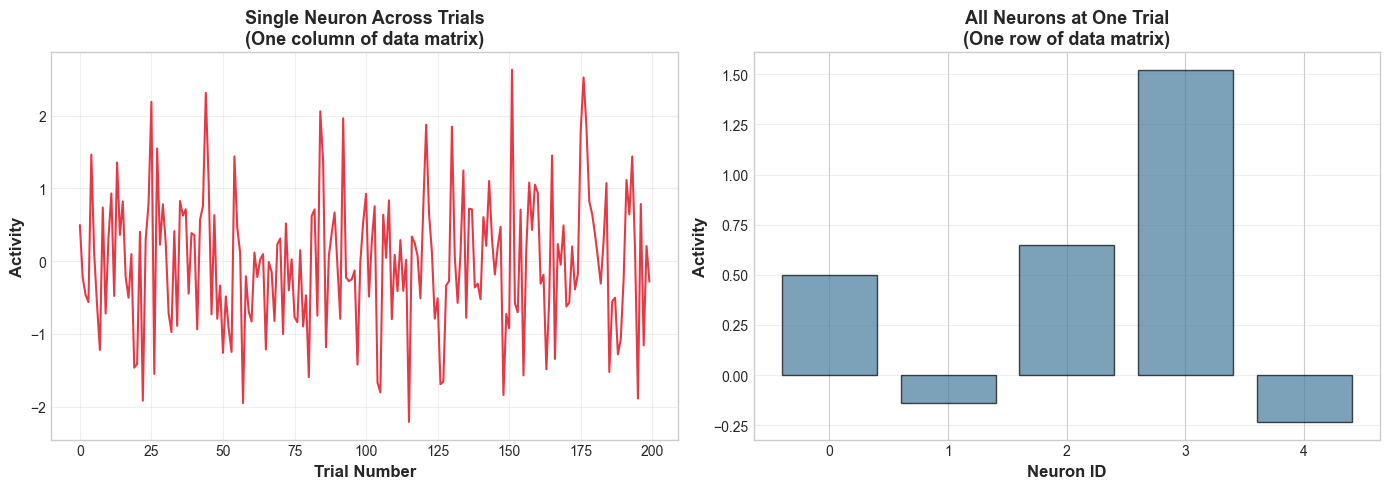
\includegraphics[keepaspectratio]{03_hoi_higher_order_interactions_files/figure-pdf/cell-4-output-2.png}}

\begin{verbatim}

💡 Key Point: HOI operates on columns (variables)
   It computes dependencies between columns using all rows as samples
\end{verbatim}

\section{Part 2: O-Information - Detecting Synergy and
Redundancy}\label{part-2-o-information---detecting-synergy-and-redundancy}

\subsection{What is O-Information?}\label{what-is-o-information}

\textbf{O-information} (``O'' stands for ``information'') extends
interaction information to any number of variables. For three variables,
it's exactly interaction information, but it generalizes beautifully to
larger systems.

For \(n\) variables \(X_1, ..., X_n\):

\[O(X_1, ..., X_n) = \text{TC}(X_1, ..., X_n) - \text{DTC}(X_1, ..., X_n)\]

Where: - \textbf{TC (Total Correlation)}:
\(\sum_i H(X_i) - H(X_1,...,X_n)\) --- measures total redundancy -
\textbf{DTC (Dual Total Correlation)}:
\(H(X_1,...,X_n) - \sum_i H(X_i|X_{-i})\) --- measures binding
information

\subsection{Interpreting the Sign}\label{interpreting-the-sign}

The beautiful thing about O-information is its sign tells you the
dominant structure:

\begin{itemize}
\tightlist
\item
  \textbf{O-info \textless{} 0 (Negative)}: \textbf{SYNERGY} dominant

  \begin{itemize}
  \tightlist
  \item
    Information emerges from combinations
  \item
    XOR-like structure
  \item
    Whole \textgreater{} sum of parts
  \end{itemize}
\item
  \textbf{O-info ≈ 0 (Zero)}: \textbf{INDEPENDENCE}

  \begin{itemize}
  \tightlist
  \item
    No higher-order structure
  \item
    Pairwise analysis sufficient
  \item
    Whole = sum of parts
  \end{itemize}
\item
  \textbf{O-info \textgreater{} 0 (Positive)}: \textbf{REDUNDANCY}
  dominant

  \begin{itemize}
  \tightlist
  \item
    Information duplicated across variables
  \item
    Common cause structure
  \item
    Whole \textless{} sum of parts
  \end{itemize}
\end{itemize}

Let's verify this works on our XOR example from Notebook 2!

\begin{Shaded}
\begin{Highlighting}[]
\CommentTok{\# Recreate XOR data}
\NormalTok{n\_samples }\OperatorTok{=} \DecValTok{1000}

\CommentTok{\# Generate independent binary variables}
\NormalTok{X1 }\OperatorTok{=}\NormalTok{ np.random.binomial(}\DecValTok{1}\NormalTok{, }\FloatTok{0.5}\NormalTok{, n\_samples)}
\NormalTok{X2 }\OperatorTok{=}\NormalTok{ np.random.binomial(}\DecValTok{1}\NormalTok{, }\FloatTok{0.5}\NormalTok{, n\_samples)}

\CommentTok{\# Create XOR output}
\NormalTok{Y }\OperatorTok{=}\NormalTok{ np.bitwise\_xor(X1, X2).astype(}\BuiltInTok{int}\NormalTok{)}

\CommentTok{\# Stack into data matrix: (n\_samples, n\_features)}
\CommentTok{\# Using column\_stack gives us (n\_samples, 3) which is correct!}
\NormalTok{data\_xor }\OperatorTok{=}\NormalTok{ np.column\_stack([X1, X2, Y])}

\BuiltInTok{print}\NormalTok{(}\StringTok{"XOR Data Created"}\NormalTok{)}
\BuiltInTok{print}\NormalTok{(}\StringTok{"="} \OperatorTok{*} \DecValTok{50}\NormalTok{)}
\BuiltInTok{print}\NormalTok{(}\SpecialStringTok{f"Data shape: }\SpecialCharTok{\{}\NormalTok{data\_xor}\SpecialCharTok{.}\NormalTok{shape}\SpecialCharTok{\}}\SpecialStringTok{"}\NormalTok{)}
\BuiltInTok{print}\NormalTok{(}\SpecialStringTok{f"  {-} }\SpecialCharTok{\{}\NormalTok{n\_samples}\SpecialCharTok{\}}\SpecialStringTok{ samples (rows)"}\NormalTok{)}
\BuiltInTok{print}\NormalTok{(}\SpecialStringTok{f"  {-} 3 variables: X₁, X₂, Y (columns)"}\NormalTok{)}
\BuiltInTok{print}\NormalTok{(}\StringTok{"}\CharTok{\textbackslash{}n}\StringTok{Verifying XOR structure:"}\NormalTok{)}
\BuiltInTok{print}\NormalTok{(}\StringTok{"Sample combinations (first 10):"}\NormalTok{)}
\ControlFlowTok{for}\NormalTok{ i }\KeywordTok{in} \BuiltInTok{range}\NormalTok{(}\DecValTok{10}\NormalTok{):}
    \BuiltInTok{print}\NormalTok{(}\SpecialStringTok{f"  X₁=}\SpecialCharTok{\{}\BuiltInTok{int}\NormalTok{(X1[i])}\SpecialCharTok{\}}\SpecialStringTok{, X₂=}\SpecialCharTok{\{}\BuiltInTok{int}\NormalTok{(X2[i])}\SpecialCharTok{\}}\SpecialStringTok{ → Y=}\SpecialCharTok{\{}\BuiltInTok{int}\NormalTok{(Y[i])}\SpecialCharTok{\}}\SpecialStringTok{"}\NormalTok{)}

\CommentTok{\# Initialize O{-}information model WITH DATA}
\CommentTok{\# HOI expects data in constructor: Oinfo(data)}
\NormalTok{model\_oinfo\_xor }\OperatorTok{=}\NormalTok{ Oinfo(data\_xor)}

\CommentTok{\# Compute O{-}information for the triplet [0, 1, 2] meaning variables X₁, X₂, Y}
\CommentTok{\# method=\textquotesingle{}binning\textquotesingle{} works well for discrete/binary data}
\NormalTok{oinfo\_xor }\OperatorTok{=}\NormalTok{ model\_oinfo\_xor.fit(method}\OperatorTok{=}\StringTok{\textquotesingle{}binning\textquotesingle{}}\NormalTok{, minsize}\OperatorTok{=}\DecValTok{3}\NormalTok{, maxsize}\OperatorTok{=}\DecValTok{3}\NormalTok{)}

\BuiltInTok{print}\NormalTok{(}\StringTok{"}\CharTok{\textbackslash{}n}\StringTok{"} \OperatorTok{+} \StringTok{"="} \OperatorTok{*} \DecValTok{50}\NormalTok{)}
\BuiltInTok{print}\NormalTok{(}\StringTok{"O{-}INFORMATION RESULT"}\NormalTok{)}
\BuiltInTok{print}\NormalTok{(}\StringTok{"="} \OperatorTok{*} \DecValTok{50}\NormalTok{)}
\BuiltInTok{print}\NormalTok{(}\SpecialStringTok{f"}\CharTok{\textbackslash{}n}\SpecialStringTok{O(X₁, X₂, Y) = }\SpecialCharTok{\{}\BuiltInTok{float}\NormalTok{(oinfo\_xor[}\DecValTok{0}\NormalTok{])}\SpecialCharTok{:.4f\}}\SpecialStringTok{ bits"}\NormalTok{)}

\ControlFlowTok{if}\NormalTok{ oinfo\_xor[}\DecValTok{0}\NormalTok{] }\OperatorTok{\textless{}} \OperatorTok{{-}}\FloatTok{0.1}\NormalTok{:}
    \BuiltInTok{print}\NormalTok{(}\StringTok{"}\CharTok{\textbackslash{}n}\StringTok{✨ NEGATIVE → SYNERGY detected!"}\NormalTok{)}
    \BuiltInTok{print}\NormalTok{(}\StringTok{"}\CharTok{\textbackslash{}n}\StringTok{Interpretation:"}\NormalTok{)}
    \BuiltInTok{print}\NormalTok{(}\StringTok{"  • Information exists only in the combination"}\NormalTok{)}
    \BuiltInTok{print}\NormalTok{(}\StringTok{"  • Neither X₁ nor X₂ alone predicts Y"}\NormalTok{)}
    \BuiltInTok{print}\NormalTok{(}\StringTok{"  • Together they predict perfectly"}\NormalTok{)}
    \BuiltInTok{print}\NormalTok{(}\StringTok{"  • This is exactly what we calculated manually in Notebook 2!"}\NormalTok{)}
\ControlFlowTok{elif}\NormalTok{ oinfo\_xor[}\DecValTok{0}\NormalTok{] }\OperatorTok{\textgreater{}} \FloatTok{0.1}\NormalTok{:}
    \BuiltInTok{print}\NormalTok{(}\StringTok{"}\CharTok{\textbackslash{}n}\StringTok{⚠️  Unexpected positive value {-} check data"}\NormalTok{)}
\ControlFlowTok{else}\NormalTok{:}
    \BuiltInTok{print}\NormalTok{(}\StringTok{"}\CharTok{\textbackslash{}n}\StringTok{⚠️  Near zero {-} might need more samples"}\NormalTok{)}

\BuiltInTok{print}\NormalTok{(}\StringTok{"}\CharTok{\textbackslash{}n}\StringTok{🎯 HOI confirmed our manual calculation!"}\NormalTok{)}
\end{Highlighting}
\end{Shaded}

\begin{verbatim}
XOR Data Created
==================================================
Data shape: (1000, 3)
  - 1000 samples (rows)
  - 3 variables: X₁, X₂, Y (columns)

Verifying XOR structure:
Sample combinations (first 10):
  X₁=0, X₂=0 → Y=0
  X₁=0, X₂=0 → Y=0
  X₁=0, X₂=1 → Y=1
  X₁=0, X₂=1 → Y=1
  X₁=0, X₂=1 → Y=1
  X₁=1, X₂=0 → Y=1
  X₁=1, X₂=1 → Y=0
  X₁=1, X₂=0 → Y=1
  X₁=0, X₂=1 → Y=1
  X₁=0, X₂=0 → Y=0
\end{verbatim}

\begin{verbatim}

==================================================
O-INFORMATION RESULT
==================================================

O(X₁, X₂, Y) = -0.9963 bits

✨ NEGATIVE → SYNERGY detected!

Interpretation:
  • Information exists only in the combination
  • Neither X₁ nor X₂ alone predicts Y
  • Together they predict perfectly
  • This is exactly what we calculated manually in Notebook 2!

🎯 HOI confirmed our manual calculation!
\end{verbatim}

\subsection{Testing with COPY (Pure
Redundancy)}\label{testing-with-copy-pure-redundancy}

Now let's verify HOI works for the opposite case - the COPY system where
information is redundant:

\begin{Shaded}
\begin{Highlighting}[]
\CommentTok{\# Create COPY data: X₂ = X₁, Y = X₁}
\NormalTok{X1\_copy }\OperatorTok{=}\NormalTok{ np.random.binomial(}\DecValTok{1}\NormalTok{, }\FloatTok{0.5}\NormalTok{, n\_samples)}
\NormalTok{X2\_copy }\OperatorTok{=}\NormalTok{ X1\_copy.copy()  }\CommentTok{\# Perfect copy}
\NormalTok{Y\_copy }\OperatorTok{=}\NormalTok{ X1\_copy.copy()   }\CommentTok{\# Y is also a copy}

\CommentTok{\# Stack into correct format (n\_samples, n\_features)}
\NormalTok{data\_copy }\OperatorTok{=}\NormalTok{ np.column\_stack([X1\_copy, X2\_copy, Y\_copy])}

\CommentTok{\# IMPORTANT: Create NEW model with the COPY data!}
\NormalTok{model\_oinfo\_copy }\OperatorTok{=}\NormalTok{ Oinfo(data\_copy)}
\NormalTok{oinfo\_copy }\OperatorTok{=}\NormalTok{ model\_oinfo\_copy.fit(method}\OperatorTok{=}\StringTok{\textquotesingle{}binning\textquotesingle{}}\NormalTok{, minsize}\OperatorTok{=}\DecValTok{3}\NormalTok{, maxsize}\OperatorTok{=}\DecValTok{3}\NormalTok{)}

\BuiltInTok{print}\NormalTok{(}\StringTok{"COPY System O{-}Information"}\NormalTok{)}
\BuiltInTok{print}\NormalTok{(}\StringTok{"="} \OperatorTok{*} \DecValTok{50}\NormalTok{)}
\BuiltInTok{print}\NormalTok{(}\SpecialStringTok{f"}\CharTok{\textbackslash{}n}\SpecialStringTok{O(X₁, X₂, Y) = }\SpecialCharTok{\{}\BuiltInTok{float}\NormalTok{(oinfo\_copy[}\DecValTok{0}\NormalTok{])}\SpecialCharTok{:.4f\}}\SpecialStringTok{ bits"}\NormalTok{)}

\ControlFlowTok{if}\NormalTok{ oinfo\_copy[}\DecValTok{0}\NormalTok{] }\OperatorTok{\textgreater{}} \FloatTok{0.1}\NormalTok{:}
    \BuiltInTok{print}\NormalTok{(}\StringTok{"}\CharTok{\textbackslash{}n}\StringTok{✨ POSITIVE → REDUNDANCY detected!"}\NormalTok{)}
    \BuiltInTok{print}\NormalTok{(}\StringTok{"}\CharTok{\textbackslash{}n}\StringTok{Interpretation:"}\NormalTok{)}
    \BuiltInTok{print}\NormalTok{(}\StringTok{"  • All three variables carry the same information"}\NormalTok{)}
    \BuiltInTok{print}\NormalTok{(}\StringTok{"  • Information is duplicated (redundant)"}\NormalTok{)}
    \BuiltInTok{print}\NormalTok{(}\StringTok{"  • Learning any one tells you about the others"}\NormalTok{)}
    \BuiltInTok{print}\NormalTok{(}\StringTok{"  • Opposite of XOR!"}\NormalTok{)}

\CommentTok{\# Compare side{-}by{-}side}
\BuiltInTok{print}\NormalTok{(}\StringTok{"}\CharTok{\textbackslash{}n}\StringTok{"} \OperatorTok{+} \StringTok{"="} \OperatorTok{*} \DecValTok{50}\NormalTok{)}
\BuiltInTok{print}\NormalTok{(}\StringTok{"XOR vs COPY Comparison"}\NormalTok{)}
\BuiltInTok{print}\NormalTok{(}\StringTok{"="} \OperatorTok{*} \DecValTok{50}\NormalTok{)}
\BuiltInTok{print}\NormalTok{(}\SpecialStringTok{f"XOR  (synergy):    O{-}info = }\SpecialCharTok{\{}\BuiltInTok{float}\NormalTok{(oinfo\_xor[}\DecValTok{0}\NormalTok{])}\SpecialCharTok{:+.4f\}}\SpecialStringTok{ bits (negative)"}\NormalTok{)}
\BuiltInTok{print}\NormalTok{(}\SpecialStringTok{f"COPY (redundancy): O{-}info = }\SpecialCharTok{\{}\BuiltInTok{float}\NormalTok{(oinfo\_copy[}\DecValTok{0}\NormalTok{])}\SpecialCharTok{:+.4f\}}\SpecialStringTok{ bits (positive)"}\NormalTok{)}
\BuiltInTok{print}\NormalTok{(}\SpecialStringTok{f"}\CharTok{\textbackslash{}n}\SpecialStringTok{Difference: }\SpecialCharTok{\{}\BuiltInTok{abs}\NormalTok{(}\BuiltInTok{float}\NormalTok{(oinfo\_xor[}\DecValTok{0}\NormalTok{]) }\OperatorTok{{-}} \BuiltInTok{float}\NormalTok{(oinfo\_copy[}\DecValTok{0}\NormalTok{]))}\SpecialCharTok{:.4f\}}\SpecialStringTok{ bits"}\NormalTok{)}
\BuiltInTok{print}\NormalTok{(}\StringTok{"}\CharTok{\textbackslash{}n}\StringTok{These are the two extremes of information structure!"}\NormalTok{)}
\end{Highlighting}
\end{Shaded}

\begin{verbatim}
COPY System O-Information
==================================================

O(X₁, X₂, Y) = 0.9997 bits

✨ POSITIVE → REDUNDANCY detected!

Interpretation:
  • All three variables carry the same information
  • Information is duplicated (redundant)
  • Learning any one tells you about the others
  • Opposite of XOR!

==================================================
XOR vs COPY Comparison
==================================================
XOR  (synergy):    O-info = -0.9963 bits (negative)
COPY (redundancy): O-info = +0.9997 bits (positive)

Difference: 1.9960 bits

These are the two extremes of information structure!
\end{verbatim}

\subsection{Visualizing the O-Information
Landscape}\label{visualizing-the-o-information-landscape}

Let's create a comprehensive visualization showing how O-information
varies across different types of systems:

\begin{Shaded}
\begin{Highlighting}[]
\CommentTok{\# Create multiple test systems with different structures}
\NormalTok{n\_samples }\OperatorTok{=} \DecValTok{5000}
\NormalTok{systems }\OperatorTok{=}\NormalTok{ \{\}}
\NormalTok{system\_methods }\OperatorTok{=}\NormalTok{ \{\}  }\CommentTok{\# Track which method to use for each system}

\CommentTok{\# 1. XOR (synergy) {-} DISCRETE, use binning}
\NormalTok{X1 }\OperatorTok{=}\NormalTok{ np.random.binomial(}\DecValTok{1}\NormalTok{, }\FloatTok{0.5}\NormalTok{, n\_samples)}
\NormalTok{X2 }\OperatorTok{=}\NormalTok{ np.random.binomial(}\DecValTok{1}\NormalTok{, }\FloatTok{0.5}\NormalTok{, n\_samples)}
\NormalTok{Y }\OperatorTok{=}\NormalTok{ np.logical\_xor(X1, X2).astype(}\BuiltInTok{int}\NormalTok{)}
\NormalTok{systems[}\StringTok{\textquotesingle{}XOR}\CharTok{\textbackslash{}n}\StringTok{(Pure Synergy)\textquotesingle{}}\NormalTok{] }\OperatorTok{=}\NormalTok{ np.column\_stack([X1, X2, Y])}
\NormalTok{system\_methods[}\StringTok{\textquotesingle{}XOR}\CharTok{\textbackslash{}n}\StringTok{(Pure Synergy)\textquotesingle{}}\NormalTok{] }\OperatorTok{=} \StringTok{\textquotesingle{}binning\textquotesingle{}}

\CommentTok{\# 2. COPY (redundancy) {-} DISCRETE, use binning}
\NormalTok{X1 }\OperatorTok{=}\NormalTok{ np.random.binomial(}\DecValTok{1}\NormalTok{, }\FloatTok{0.5}\NormalTok{, n\_samples)}
\NormalTok{systems[}\StringTok{\textquotesingle{}COPY}\CharTok{\textbackslash{}n}\StringTok{(Pure Redundancy)\textquotesingle{}}\NormalTok{] }\OperatorTok{=}\NormalTok{ np.column\_stack([X1, X1, X1]).astype(}\BuiltInTok{int}\NormalTok{)}
\NormalTok{system\_methods[}\StringTok{\textquotesingle{}COPY}\CharTok{\textbackslash{}n}\StringTok{(Pure Redundancy)\textquotesingle{}}\NormalTok{] }\OperatorTok{=} \StringTok{\textquotesingle{}binning\textquotesingle{}}

\CommentTok{\# 3. Common cause (partial redundancy) {-} CONTINUOUS, use gc}
\NormalTok{Z }\OperatorTok{=}\NormalTok{ np.random.randn(n\_samples)}
\NormalTok{X1 }\OperatorTok{=}\NormalTok{ Z }\OperatorTok{+}\NormalTok{ np.random.randn(n\_samples) }\OperatorTok{*} \FloatTok{0.5}
\NormalTok{X2 }\OperatorTok{=}\NormalTok{ Z }\OperatorTok{+}\NormalTok{ np.random.randn(n\_samples) }\OperatorTok{*} \FloatTok{0.5}
\NormalTok{Y }\OperatorTok{=}\NormalTok{ Z }\OperatorTok{+}\NormalTok{ np.random.randn(n\_samples) }\OperatorTok{*} \FloatTok{0.5}
\NormalTok{systems[}\StringTok{\textquotesingle{}Common Cause}\CharTok{\textbackslash{}n}\StringTok{(Moderate Redundancy)\textquotesingle{}}\NormalTok{] }\OperatorTok{=}\NormalTok{ np.column\_stack([X1, X2, Y]).astype(}\BuiltInTok{float}\NormalTok{)}
\NormalTok{system\_methods[}\StringTok{\textquotesingle{}Common Cause}\CharTok{\textbackslash{}n}\StringTok{(Moderate Redundancy)\textquotesingle{}}\NormalTok{] }\OperatorTok{=} \StringTok{\textquotesingle{}gc\textquotesingle{}}

\CommentTok{\# 4. Independent {-} CONTINUOUS, use gc}
\NormalTok{X1 }\OperatorTok{=}\NormalTok{ np.random.randn(n\_samples)}
\NormalTok{X2 }\OperatorTok{=}\NormalTok{ np.random.randn(n\_samples)}
\NormalTok{Y }\OperatorTok{=}\NormalTok{ np.random.randn(n\_samples)}
\NormalTok{systems[}\StringTok{\textquotesingle{}Independent}\CharTok{\textbackslash{}n}\StringTok{(No Structure)\textquotesingle{}}\NormalTok{] }\OperatorTok{=}\NormalTok{ np.column\_stack([X1, X2, Y]).astype(}\BuiltInTok{float}\NormalTok{)}
\NormalTok{system\_methods[}\StringTok{\textquotesingle{}Independent}\CharTok{\textbackslash{}n}\StringTok{(No Structure)\textquotesingle{}}\NormalTok{] }\OperatorTok{=} \StringTok{\textquotesingle{}gc\textquotesingle{}}

\CommentTok{\# 5. Partial synergy (XOR with noise) {-} DISCRETE, use binning}
\NormalTok{X1 }\OperatorTok{=}\NormalTok{ np.random.binomial(}\DecValTok{1}\NormalTok{, }\FloatTok{0.5}\NormalTok{, n\_samples)}
\NormalTok{X2 }\OperatorTok{=}\NormalTok{ np.random.binomial(}\DecValTok{1}\NormalTok{, }\FloatTok{0.5}\NormalTok{, n\_samples)}
\NormalTok{Y\_clean }\OperatorTok{=}\NormalTok{ np.logical\_xor(X1, X2)}
\CommentTok{\# Add noise by flipping 20\% of bits}
\NormalTok{flip\_mask }\OperatorTok{=}\NormalTok{ np.random.rand(n\_samples) }\OperatorTok{\textless{}} \FloatTok{0.2}
\NormalTok{Y }\OperatorTok{=}\NormalTok{ np.logical\_xor(Y\_clean, flip\_mask).astype(}\BuiltInTok{int}\NormalTok{)}
\NormalTok{systems[}\StringTok{\textquotesingle{}Noisy XOR}\CharTok{\textbackslash{}n}\StringTok{(Partial Synergy)\textquotesingle{}}\NormalTok{] }\OperatorTok{=}\NormalTok{ np.column\_stack([X1, X2, Y]).astype(}\BuiltInTok{int}\NormalTok{)}
\NormalTok{system\_methods[}\StringTok{\textquotesingle{}Noisy XOR}\CharTok{\textbackslash{}n}\StringTok{(Partial Synergy)\textquotesingle{}}\NormalTok{] }\OperatorTok{=} \StringTok{\textquotesingle{}binning\textquotesingle{}}

\CommentTok{\# 6. AND gate (between XOR and COPY) {-} DISCRETE, use binning}
\NormalTok{X1 }\OperatorTok{=}\NormalTok{ np.random.binomial(}\DecValTok{1}\NormalTok{, }\FloatTok{0.5}\NormalTok{, n\_samples)}
\NormalTok{X2 }\OperatorTok{=}\NormalTok{ np.random.binomial(}\DecValTok{1}\NormalTok{, }\FloatTok{0.5}\NormalTok{, n\_samples)}
\NormalTok{Y }\OperatorTok{=}\NormalTok{ np.logical\_and(X1, X2).astype(}\BuiltInTok{int}\NormalTok{)}
\NormalTok{systems[}\StringTok{\textquotesingle{}AND Gate}\CharTok{\textbackslash{}n}\StringTok{(Mixed)\textquotesingle{}}\NormalTok{] }\OperatorTok{=}\NormalTok{ np.column\_stack([X1, X2, Y]).astype(}\BuiltInTok{int}\NormalTok{)}
\NormalTok{system\_methods[}\StringTok{\textquotesingle{}AND Gate}\CharTok{\textbackslash{}n}\StringTok{(Mixed)\textquotesingle{}}\NormalTok{] }\OperatorTok{=} \StringTok{\textquotesingle{}binning\textquotesingle{}}

\CommentTok{\# Compute O{-}information for all systems}
\CommentTok{\# IMPORTANT: Use the appropriate method for each data type!}
\NormalTok{oinfo\_values }\OperatorTok{=}\NormalTok{ \{\}}
\ControlFlowTok{for}\NormalTok{ name, data }\KeywordTok{in}\NormalTok{ systems.items():}
\NormalTok{    method }\OperatorTok{=}\NormalTok{ system\_methods[name]}
\NormalTok{    model }\OperatorTok{=}\NormalTok{ Oinfo(data)}
\NormalTok{    oinfo }\OperatorTok{=}\NormalTok{ model.fit(method}\OperatorTok{=}\NormalTok{method, minsize}\OperatorTok{=}\DecValTok{3}\NormalTok{, maxsize}\OperatorTok{=}\DecValTok{3}\NormalTok{)}
\NormalTok{    oinfo\_values[name] }\OperatorTok{=} \BuiltInTok{float}\NormalTok{(oinfo[}\DecValTok{0}\NormalTok{])}
    \BuiltInTok{print}\NormalTok{(}\SpecialStringTok{f"✓ }\SpecialCharTok{\{}\NormalTok{name}\SpecialCharTok{.}\NormalTok{replace(}\BuiltInTok{chr}\NormalTok{(}\DecValTok{10}\NormalTok{), }\StringTok{\textquotesingle{} \textquotesingle{}}\NormalTok{)}\SpecialCharTok{\}}\SpecialStringTok{: O{-}info = }\SpecialCharTok{\{}\BuiltInTok{float}\NormalTok{(oinfo[}\DecValTok{0}\NormalTok{])}\SpecialCharTok{:.4f\}}\SpecialStringTok{ (method=}\SpecialCharTok{\{}\NormalTok{method}\SpecialCharTok{\}}\SpecialStringTok{)"}\NormalTok{)}

\CommentTok{\# Create visualization}
\NormalTok{fig, (ax1, ax2) }\OperatorTok{=}\NormalTok{ plt.subplots(}\DecValTok{1}\NormalTok{, }\DecValTok{2}\NormalTok{, figsize}\OperatorTok{=}\NormalTok{(}\DecValTok{16}\NormalTok{, }\DecValTok{6}\NormalTok{))}

\CommentTok{\# Plot 1: Bar chart}
\NormalTok{names }\OperatorTok{=} \BuiltInTok{list}\NormalTok{(oinfo\_values.keys())}
\NormalTok{values }\OperatorTok{=} \BuiltInTok{list}\NormalTok{(oinfo\_values.values())}
\NormalTok{colors }\OperatorTok{=}\NormalTok{ [}\StringTok{\textquotesingle{}red\textquotesingle{}} \ControlFlowTok{if}\NormalTok{ v }\OperatorTok{\textless{}} \OperatorTok{{-}}\FloatTok{0.1} \ControlFlowTok{else} \StringTok{\textquotesingle{}gray\textquotesingle{}} \ControlFlowTok{if} \BuiltInTok{abs}\NormalTok{(v) }\OperatorTok{\textless{}} \FloatTok{0.1} \ControlFlowTok{else} \StringTok{\textquotesingle{}blue\textquotesingle{}} \ControlFlowTok{for}\NormalTok{ v }\KeywordTok{in}\NormalTok{ values]}

\NormalTok{bars }\OperatorTok{=}\NormalTok{ ax1.barh(names, values, color}\OperatorTok{=}\NormalTok{colors, alpha}\OperatorTok{=}\FloatTok{0.7}\NormalTok{, edgecolor}\OperatorTok{=}\StringTok{\textquotesingle{}black\textquotesingle{}}\NormalTok{, linewidth}\OperatorTok{=}\DecValTok{2}\NormalTok{)}
\NormalTok{ax1.axvline(x}\OperatorTok{=}\DecValTok{0}\NormalTok{, color}\OperatorTok{=}\StringTok{\textquotesingle{}black\textquotesingle{}}\NormalTok{, linestyle}\OperatorTok{=}\StringTok{\textquotesingle{}{-}\textquotesingle{}}\NormalTok{, linewidth}\OperatorTok{=}\DecValTok{2}\NormalTok{)}
\NormalTok{ax1.axvline(x}\OperatorTok{={-}}\FloatTok{0.1}\NormalTok{, color}\OperatorTok{=}\StringTok{\textquotesingle{}red\textquotesingle{}}\NormalTok{, linestyle}\OperatorTok{=}\StringTok{\textquotesingle{}{-}{-}\textquotesingle{}}\NormalTok{, alpha}\OperatorTok{=}\FloatTok{0.5}\NormalTok{, label}\OperatorTok{=}\StringTok{\textquotesingle{}Synergy threshold\textquotesingle{}}\NormalTok{)}
\NormalTok{ax1.axvline(x}\OperatorTok{=}\FloatTok{0.1}\NormalTok{, color}\OperatorTok{=}\StringTok{\textquotesingle{}blue\textquotesingle{}}\NormalTok{, linestyle}\OperatorTok{=}\StringTok{\textquotesingle{}{-}{-}\textquotesingle{}}\NormalTok{, alpha}\OperatorTok{=}\FloatTok{0.5}\NormalTok{, label}\OperatorTok{=}\StringTok{\textquotesingle{}Redundancy threshold\textquotesingle{}}\NormalTok{)}
\NormalTok{ax1.set\_xlabel(}\StringTok{\textquotesingle{}O{-}Information (bits)\textquotesingle{}}\NormalTok{, fontsize}\OperatorTok{=}\DecValTok{14}\NormalTok{, fontweight}\OperatorTok{=}\StringTok{\textquotesingle{}bold\textquotesingle{}}\NormalTok{)}
\NormalTok{ax1.set\_title(}\StringTok{\textquotesingle{}O{-}Information Across Different Systems\textquotesingle{}}\NormalTok{, fontsize}\OperatorTok{=}\DecValTok{16}\NormalTok{, fontweight}\OperatorTok{=}\StringTok{\textquotesingle{}bold\textquotesingle{}}\NormalTok{)}
\NormalTok{ax1.legend(loc}\OperatorTok{=}\StringTok{\textquotesingle{}lower right\textquotesingle{}}\NormalTok{)}
\NormalTok{ax1.grid(}\VariableTok{True}\NormalTok{, alpha}\OperatorTok{=}\FloatTok{0.3}\NormalTok{, axis}\OperatorTok{=}\StringTok{\textquotesingle{}x\textquotesingle{}}\NormalTok{)}

\CommentTok{\# Add value labels}
\ControlFlowTok{for}\NormalTok{ bar, val }\KeywordTok{in} \BuiltInTok{zip}\NormalTok{(bars, values):}
\NormalTok{    xpos }\OperatorTok{=}\NormalTok{ val }\OperatorTok{+} \FloatTok{0.02} \ControlFlowTok{if}\NormalTok{ val }\OperatorTok{\textgreater{}=} \DecValTok{0} \ControlFlowTok{else}\NormalTok{ val }\OperatorTok{{-}} \FloatTok{0.02}
\NormalTok{    ha }\OperatorTok{=} \StringTok{\textquotesingle{}left\textquotesingle{}} \ControlFlowTok{if}\NormalTok{ val }\OperatorTok{\textgreater{}=} \DecValTok{0} \ControlFlowTok{else} \StringTok{\textquotesingle{}right\textquotesingle{}}
\NormalTok{    ax1.text(xpos, bar.get\_y() }\OperatorTok{+}\NormalTok{ bar.get\_height()}\OperatorTok{/}\DecValTok{2}\NormalTok{, }\SpecialStringTok{f\textquotesingle{}}\SpecialCharTok{\{}\NormalTok{val}\SpecialCharTok{:.3f\}}\SpecialStringTok{\textquotesingle{}}\NormalTok{, }
\NormalTok{             va}\OperatorTok{=}\StringTok{\textquotesingle{}center\textquotesingle{}}\NormalTok{, ha}\OperatorTok{=}\NormalTok{ha, fontweight}\OperatorTok{=}\StringTok{\textquotesingle{}bold\textquotesingle{}}\NormalTok{, fontsize}\OperatorTok{=}\DecValTok{10}\NormalTok{)}

\CommentTok{\# Plot 2: Interpretation guide}
\NormalTok{ax2.axis(}\StringTok{\textquotesingle{}off\textquotesingle{}}\NormalTok{)}
\NormalTok{interpretation\_text }\OperatorTok{=} \StringTok{"""}
\StringTok{INTERPRETING O{-}INFORMATION}

\StringTok{SYNERGY (O{-}info \textless{} 0):}
\StringTok{━━━━━━━━━━━━━━━━━━━━━}
\StringTok{• Information emerges from combinations}
\StringTok{• Knowing individual variables doesn\textquotesingle{}t help}
\StringTok{• "The whole is greater than the sum of parts"}
\StringTok{• Example: XOR gate}

\StringTok{INDEPENDENCE (O{-}info ≈ 0):}
\StringTok{━━━━━━━━━━━━━━━━━━━━━━━━━}
\StringTok{• No higher{-}order structure}
\StringTok{• Variables are essentially independent}
\StringTok{• Pairwise analysis is sufficient}

\StringTok{REDUNDANCY (O{-}info \textgreater{} 0):}
\StringTok{━━━━━━━━━━━━━━━━━━━━━━━}
\StringTok{• Information is duplicated}
\StringTok{• Multiple variables carry same info}
\StringTok{• "The whole is less than sum of parts"}
\StringTok{• Example: COPY operation}

\StringTok{ESTIMATOR CHOICE:}
\StringTok{━━━━━━━━━━━━━━━━━}
\StringTok{• \textquotesingle{}binning\textquotesingle{} → discrete/binary data (requires int)}
\StringTok{• \textquotesingle{}gc\textquotesingle{} → continuous data (Gaussian copula)}
\StringTok{• \textquotesingle{}gauss\textquotesingle{} → Gaussian data only}
\StringTok{"""}
\NormalTok{ax2.text(}\FloatTok{0.1}\NormalTok{, }\FloatTok{0.5}\NormalTok{, interpretation\_text, fontsize}\OperatorTok{=}\DecValTok{11}\NormalTok{, fontfamily}\OperatorTok{=}\StringTok{\textquotesingle{}monospace\textquotesingle{}}\NormalTok{,}
\NormalTok{         verticalalignment}\OperatorTok{=}\StringTok{\textquotesingle{}center\textquotesingle{}}\NormalTok{, transform}\OperatorTok{=}\NormalTok{ax2.transAxes,}
\NormalTok{         bbox}\OperatorTok{=}\BuiltInTok{dict}\NormalTok{(boxstyle}\OperatorTok{=}\StringTok{\textquotesingle{}round\textquotesingle{}}\NormalTok{, facecolor}\OperatorTok{=}\StringTok{\textquotesingle{}wheat\textquotesingle{}}\NormalTok{, alpha}\OperatorTok{=}\FloatTok{0.5}\NormalTok{))}

\NormalTok{plt.tight\_layout()}
\NormalTok{plt.show()}

\BuiltInTok{print}\NormalTok{(}\StringTok{"}\CharTok{\textbackslash{}n}\StringTok{📊 Summary of Results:"}\NormalTok{)}
\BuiltInTok{print}\NormalTok{(}\StringTok{"="} \OperatorTok{*} \DecValTok{60}\NormalTok{)}
\ControlFlowTok{for}\NormalTok{ name, val }\KeywordTok{in}\NormalTok{ oinfo\_values.items():}
\NormalTok{    category }\OperatorTok{=} \StringTok{"SYNERGY"} \ControlFlowTok{if}\NormalTok{ val }\OperatorTok{\textless{}} \OperatorTok{{-}}\FloatTok{0.1} \ControlFlowTok{else} \StringTok{"INDEPENDENCE"} \ControlFlowTok{if} \BuiltInTok{abs}\NormalTok{(val) }\OperatorTok{\textless{}} \FloatTok{0.1} \ControlFlowTok{else} \StringTok{"REDUNDANCY"}
    \BuiltInTok{print}\NormalTok{(}\SpecialStringTok{f"}\SpecialCharTok{\{}\NormalTok{name}\SpecialCharTok{.}\NormalTok{replace(}\BuiltInTok{chr}\NormalTok{(}\DecValTok{10}\NormalTok{), }\StringTok{\textquotesingle{} \textquotesingle{}}\NormalTok{)}\SpecialCharTok{:30s\}}\SpecialStringTok{: }\SpecialCharTok{\{}\NormalTok{val}\SpecialCharTok{:+.4f\}}\SpecialStringTok{ bits → }\SpecialCharTok{\{}\NormalTok{category}\SpecialCharTok{\}}\SpecialStringTok{"}\NormalTok{)}
\end{Highlighting}
\end{Shaded}

\begin{verbatim}
✓ XOR (Pure Synergy): O-info = -0.9991 (method=binning)
\end{verbatim}

\begin{verbatim}
✓ COPY (Pure Redundancy): O-info = 0.9994 (method=binning)
\end{verbatim}

\begin{verbatim}
✓ Common Cause (Moderate Redundancy): O-info = 0.5634 (method=gc)
\end{verbatim}

\begin{verbatim}
✓ Independent (No Structure): O-info = -0.0000 (method=gc)
\end{verbatim}

\begin{verbatim}
✓ Noisy XOR (Partial Synergy): O-info = -0.2893 (method=binning)
\end{verbatim}

\begin{verbatim}
✓ AND Gate (Mixed): O-info = -0.1831 (method=binning)
\end{verbatim}

\pandocbounded{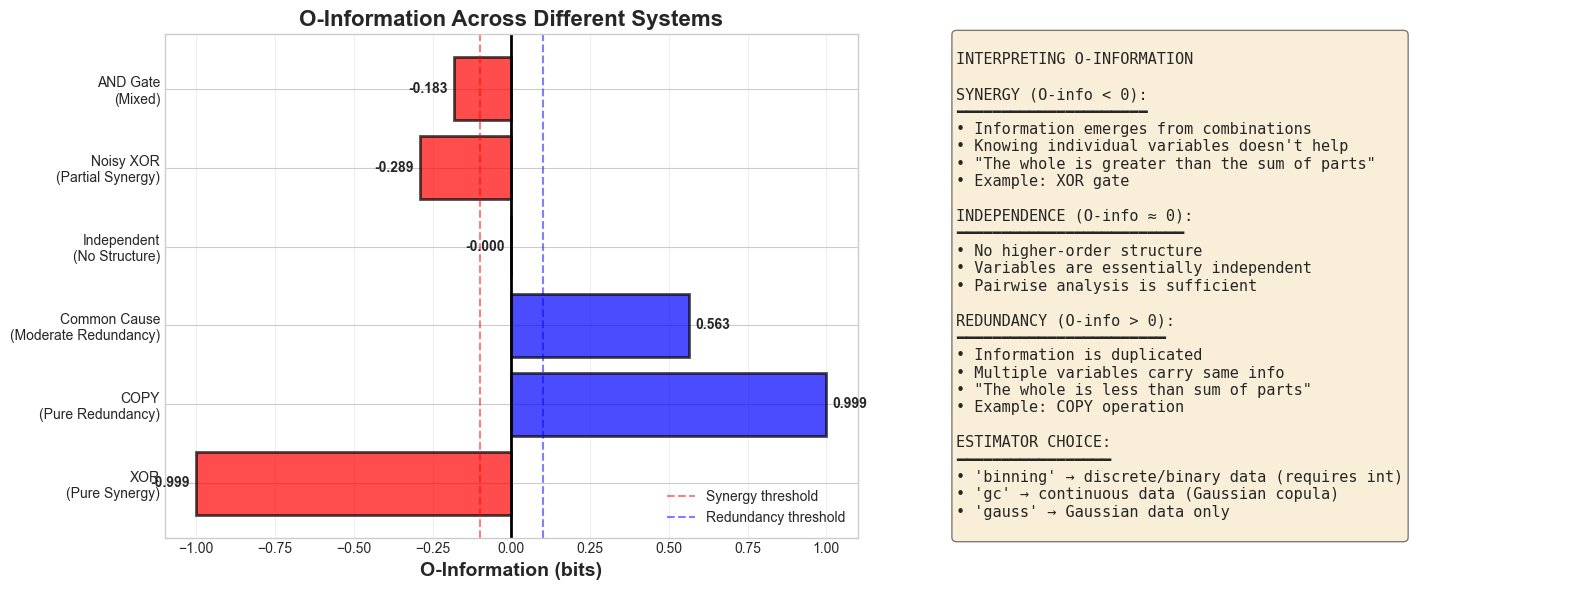
\includegraphics[keepaspectratio]{03_hoi_higher_order_interactions_files/figure-pdf/cell-7-output-7.png}}

\begin{verbatim}

📊 Summary of Results:
============================================================
XOR (Pure Synergy)            : -0.9991 bits → SYNERGY
COPY (Pure Redundancy)        : +0.9994 bits → REDUNDANCY
Common Cause (Moderate Redundancy): +0.5634 bits → REDUNDANCY
Independent (No Structure)    : -0.0000 bits → INDEPENDENCE
Noisy XOR (Partial Synergy)   : -0.2893 bits → SYNERGY
AND Gate (Mixed)              : -0.1831 bits → SYNERGY
\end{verbatim}

\section{Part 3: Understanding Different
Estimators}\label{part-3-understanding-different-estimators}

\subsection{Why Estimators Matter}\label{why-estimators-matter}

HOI provides multiple methods for estimating information quantities.
Each has trade-offs between: - \textbf{Accuracy}: How close to true
value? - \textbf{Bias}: Systematic over/underestimation? -
\textbf{Variance}: How much do estimates fluctuate with different
samples? - \textbf{Computational cost}: How fast? -
\textbf{Assumptions}: What data types work?

\subsection{Available Estimators in
HOI}\label{available-estimators-in-hoi}

\begin{enumerate}
\def\labelenumi{\arabic{enumi}.}
\tightlist
\item
  \textbf{`gc' (Gaussian Copula)}:

  \begin{itemize}
  \tightlist
  \item
    Works for any data type
  \item
    Fast and accurate
  \item
    Assumes monotonic relationships
  \item
    \textbf{Recommended default}
  \end{itemize}
\item
  \textbf{`gauss' (Gaussian)}:

  \begin{itemize}
  \tightlist
  \item
    Assumes data is Gaussian
  \item
    Very fast
  \item
    Only use if data is truly normal
  \end{itemize}
\item
  \textbf{`binning' (Histogram)}:

  \begin{itemize}
  \tightlist
  \item
    Simple and intuitive
  \item
    Requires choosing bin count
  \item
    Can be biased
  \end{itemize}
\item
  \textbf{`knn' (K-Nearest Neighbors)}:

  \begin{itemize}
  \tightlist
  \item
    Non-parametric
  \item
    Works for any distribution
  \item
    Can be slow for large datasets
  \end{itemize}
\item
  \textbf{`kernel' (Kernel Density)}:

  \begin{itemize}
  \tightlist
  \item
    Smooth estimation
  \item
    Requires bandwidth selection
  \item
    Good for continuous data
  \end{itemize}
\end{enumerate}

Let's test different estimators on the same XOR data to see how they
compare:

\begin{Shaded}
\begin{Highlighting}[]
\CommentTok{\# Test different estimators on XOR data}
\NormalTok{estimators }\OperatorTok{=}\NormalTok{ [}\StringTok{\textquotesingle{}gc\textquotesingle{}}\NormalTok{, }\StringTok{\textquotesingle{}gauss\textquotesingle{}}\NormalTok{, }\StringTok{\textquotesingle{}binning\textquotesingle{}}\NormalTok{, }\StringTok{\textquotesingle{}knn\textquotesingle{}}\NormalTok{]}
\NormalTok{estimator\_results }\OperatorTok{=}\NormalTok{ \{\}}

\BuiltInTok{print}\NormalTok{(}\StringTok{"Comparing Estimators on XOR Data"}\NormalTok{)}
\BuiltInTok{print}\NormalTok{(}\StringTok{"="} \OperatorTok{*} \DecValTok{60}\NormalTok{)}
\BuiltInTok{print}\NormalTok{(}\SpecialStringTok{f"Data: }\SpecialCharTok{\{}\NormalTok{data\_xor}\SpecialCharTok{.}\NormalTok{shape[}\DecValTok{0}\NormalTok{]}\SpecialCharTok{\}}\SpecialStringTok{ samples, binary XOR structure}\CharTok{\textbackslash{}n}\SpecialStringTok{"}\NormalTok{)}

\ImportTok{import}\NormalTok{ time}

\ControlFlowTok{for}\NormalTok{ method }\KeywordTok{in}\NormalTok{ estimators:}
    \ControlFlowTok{try}\NormalTok{:}
        \CommentTok{\# IMPORTANT: Create model WITH DATA, then specify method in fit()}
\NormalTok{        model }\OperatorTok{=}\NormalTok{ Oinfo(data\_xor)}
        
        \CommentTok{\# Time the computation}
\NormalTok{        start }\OperatorTok{=}\NormalTok{ time.time()}
\NormalTok{        oinfo }\OperatorTok{=}\NormalTok{ model.fit(method}\OperatorTok{=}\NormalTok{method, minsize}\OperatorTok{=}\DecValTok{3}\NormalTok{, maxsize}\OperatorTok{=}\DecValTok{3}\NormalTok{)}
\NormalTok{        elapsed }\OperatorTok{=}\NormalTok{ time.time() }\OperatorTok{{-}}\NormalTok{ start}
        
\NormalTok{        estimator\_results[method] }\OperatorTok{=}\NormalTok{ \{}
            \StringTok{\textquotesingle{}value\textquotesingle{}}\NormalTok{: }\BuiltInTok{float}\NormalTok{(oinfo[}\DecValTok{0}\NormalTok{]),}
            \StringTok{\textquotesingle{}time\textquotesingle{}}\NormalTok{: elapsed}
\NormalTok{        \}}
        
        \BuiltInTok{print}\NormalTok{(}\SpecialStringTok{f"}\SpecialCharTok{\{}\NormalTok{method}\SpecialCharTok{:12s\}}\SpecialStringTok{: O{-}info = }\SpecialCharTok{\{}\NormalTok{oinfo[}\DecValTok{0}\NormalTok{]}\SpecialCharTok{:+.4f\}}\SpecialStringTok{ bits  (time: }\SpecialCharTok{\{}\NormalTok{elapsed}\SpecialCharTok{:.4f\}}\SpecialStringTok{s)"}\NormalTok{)}
        
    \ControlFlowTok{except} \PreprocessorTok{Exception} \ImportTok{as}\NormalTok{ e:}
        \BuiltInTok{print}\NormalTok{(}\SpecialStringTok{f"}\SpecialCharTok{\{}\NormalTok{method}\SpecialCharTok{:12s\}}\SpecialStringTok{: Failed {-} }\SpecialCharTok{\{}\BuiltInTok{str}\NormalTok{(e)[:}\DecValTok{50}\NormalTok{]}\SpecialCharTok{\}}\SpecialStringTok{"}\NormalTok{)}

\CommentTok{\# Analyze results}
\BuiltInTok{print}\NormalTok{(}\StringTok{"}\CharTok{\textbackslash{}n}\StringTok{"} \OperatorTok{+} \StringTok{"="} \OperatorTok{*} \DecValTok{60}\NormalTok{)}
\BuiltInTok{print}\NormalTok{(}\StringTok{"Analysis:"}\NormalTok{)}
\BuiltInTok{print}\NormalTok{(}\StringTok{"="} \OperatorTok{*} \DecValTok{60}\NormalTok{)}

\ControlFlowTok{if} \StringTok{\textquotesingle{}gc\textquotesingle{}} \KeywordTok{in}\NormalTok{ estimator\_results }\KeywordTok{and} \StringTok{\textquotesingle{}gauss\textquotesingle{}} \KeywordTok{in}\NormalTok{ estimator\_results:}
\NormalTok{    gc\_val }\OperatorTok{=}\NormalTok{ estimator\_results[}\StringTok{\textquotesingle{}gc\textquotesingle{}}\NormalTok{][}\StringTok{\textquotesingle{}value\textquotesingle{}}\NormalTok{]}
\NormalTok{    gauss\_val }\OperatorTok{=}\NormalTok{ estimator\_results[}\StringTok{\textquotesingle{}gauss\textquotesingle{}}\NormalTok{][}\StringTok{\textquotesingle{}value\textquotesingle{}}\NormalTok{]}
    \BuiltInTok{print}\NormalTok{(}\SpecialStringTok{f"}\CharTok{\textbackslash{}n}\SpecialStringTok{Gaussian Copula (gc): }\SpecialCharTok{\{}\NormalTok{gc\_val}\SpecialCharTok{:.4f\}}\SpecialStringTok{ bits"}\NormalTok{)}
    \BuiltInTok{print}\NormalTok{(}\SpecialStringTok{f"Gaussian (gauss):     }\SpecialCharTok{\{}\NormalTok{gauss\_val}\SpecialCharTok{:.4f\}}\SpecialStringTok{ bits"}\NormalTok{)}
    \BuiltInTok{print}\NormalTok{(}\SpecialStringTok{f"Difference: }\SpecialCharTok{\{}\BuiltInTok{abs}\NormalTok{(gc\_val }\OperatorTok{{-}}\NormalTok{ gauss\_val)}\SpecialCharTok{:.4f\}}\SpecialStringTok{ bits"}\NormalTok{)}
    \BuiltInTok{print}\NormalTok{(}\StringTok{"}\CharTok{\textbackslash{}n}\StringTok{💡 \textquotesingle{}gc\textquotesingle{} is usually more accurate for non{-}Gaussian data"}\NormalTok{)}
    \BuiltInTok{print}\NormalTok{(}\StringTok{"   \textquotesingle{}gauss\textquotesingle{} is faster but assumes normality"}\NormalTok{)}

\ControlFlowTok{if} \StringTok{\textquotesingle{}binning\textquotesingle{}} \KeywordTok{in}\NormalTok{ estimator\_results:}
    \BuiltInTok{print}\NormalTok{(}\SpecialStringTok{f"}\CharTok{\textbackslash{}n}\SpecialStringTok{Binning: }\SpecialCharTok{\{}\NormalTok{estimator\_results[}\StringTok{\textquotesingle{}binning\textquotesingle{}}\NormalTok{][}\StringTok{\textquotesingle{}value\textquotesingle{}}\NormalTok{]}\SpecialCharTok{:.4f\}}\SpecialStringTok{ bits"}\NormalTok{)}
    \BuiltInTok{print}\NormalTok{(}\StringTok{"✓ Binning works well for discrete/binary data like XOR"}\NormalTok{)}

\CommentTok{\# Visualize comparison}
\ControlFlowTok{if} \BuiltInTok{len}\NormalTok{(estimator\_results) }\OperatorTok{\textgreater{}} \DecValTok{1}\NormalTok{:}
\NormalTok{    fig, (ax1, ax2) }\OperatorTok{=}\NormalTok{ plt.subplots(}\DecValTok{1}\NormalTok{, }\DecValTok{2}\NormalTok{, figsize}\OperatorTok{=}\NormalTok{(}\DecValTok{14}\NormalTok{, }\DecValTok{5}\NormalTok{))}
    
    \CommentTok{\# Plot 1: O{-}info values}
\NormalTok{    methods }\OperatorTok{=} \BuiltInTok{list}\NormalTok{(estimator\_results.keys())}
\NormalTok{    values }\OperatorTok{=}\NormalTok{ [estimator\_results[m][}\StringTok{\textquotesingle{}value\textquotesingle{}}\NormalTok{] }\ControlFlowTok{for}\NormalTok{ m }\KeywordTok{in}\NormalTok{ methods]}
    
\NormalTok{    colors }\OperatorTok{=}\NormalTok{ [}\StringTok{\textquotesingle{}\#E63946\textquotesingle{}}\NormalTok{, }\StringTok{\textquotesingle{}\#457B9D\textquotesingle{}}\NormalTok{, }\StringTok{\textquotesingle{}\#A8DADC\textquotesingle{}}\NormalTok{, }\StringTok{\textquotesingle{}\#F1FAEE\textquotesingle{}}\NormalTok{][:}\BuiltInTok{len}\NormalTok{(methods)]}
\NormalTok{    ax1.bar(methods, values, color}\OperatorTok{=}\NormalTok{colors, alpha}\OperatorTok{=}\FloatTok{0.7}\NormalTok{, edgecolor}\OperatorTok{=}\StringTok{\textquotesingle{}black\textquotesingle{}}\NormalTok{, linewidth}\OperatorTok{=}\DecValTok{2}\NormalTok{)}
\NormalTok{    ax1.axhline(y}\OperatorTok{=}\DecValTok{0}\NormalTok{, color}\OperatorTok{=}\StringTok{\textquotesingle{}black\textquotesingle{}}\NormalTok{, linestyle}\OperatorTok{=}\StringTok{\textquotesingle{}{-}\textquotesingle{}}\NormalTok{, linewidth}\OperatorTok{=}\DecValTok{2}\NormalTok{)}
\NormalTok{    ax1.set\_ylabel(}\StringTok{\textquotesingle{}O{-}Information (bits)\textquotesingle{}}\NormalTok{, fontsize}\OperatorTok{=}\DecValTok{12}\NormalTok{, fontweight}\OperatorTok{=}\StringTok{\textquotesingle{}bold\textquotesingle{}}\NormalTok{)}
\NormalTok{    ax1.set\_title(}\StringTok{\textquotesingle{}Estimator Comparison: O{-}info Values\textquotesingle{}}\NormalTok{, fontsize}\OperatorTok{=}\DecValTok{14}\NormalTok{, fontweight}\OperatorTok{=}\StringTok{\textquotesingle{}bold\textquotesingle{}}\NormalTok{)}
\NormalTok{    ax1.grid(}\VariableTok{True}\NormalTok{, alpha}\OperatorTok{=}\FloatTok{0.3}\NormalTok{, axis}\OperatorTok{=}\StringTok{\textquotesingle{}y\textquotesingle{}}\NormalTok{)}
    
    \CommentTok{\# Plot 2: Computation time}
\NormalTok{    times }\OperatorTok{=}\NormalTok{ [estimator\_results[m][}\StringTok{\textquotesingle{}time\textquotesingle{}}\NormalTok{]}\OperatorTok{*}\DecValTok{1000} \ControlFlowTok{for}\NormalTok{ m }\KeywordTok{in}\NormalTok{ methods]}
\NormalTok{    ax2.bar(methods, times, color}\OperatorTok{=}\NormalTok{colors, alpha}\OperatorTok{=}\FloatTok{0.7}\NormalTok{, edgecolor}\OperatorTok{=}\StringTok{\textquotesingle{}black\textquotesingle{}}\NormalTok{, linewidth}\OperatorTok{=}\DecValTok{2}\NormalTok{)}
\NormalTok{    ax2.set\_ylabel(}\StringTok{\textquotesingle{}Time (ms)\textquotesingle{}}\NormalTok{, fontsize}\OperatorTok{=}\DecValTok{12}\NormalTok{, fontweight}\OperatorTok{=}\StringTok{\textquotesingle{}bold\textquotesingle{}}\NormalTok{)}
\NormalTok{    ax2.set\_title(}\StringTok{\textquotesingle{}Estimator Comparison: Computation Time\textquotesingle{}}\NormalTok{, fontsize}\OperatorTok{=}\DecValTok{14}\NormalTok{, fontweight}\OperatorTok{=}\StringTok{\textquotesingle{}bold\textquotesingle{}}\NormalTok{)}
\NormalTok{    ax2.grid(}\VariableTok{True}\NormalTok{, alpha}\OperatorTok{=}\FloatTok{0.3}\NormalTok{, axis}\OperatorTok{=}\StringTok{\textquotesingle{}y\textquotesingle{}}\NormalTok{)}
    
\NormalTok{    plt.tight\_layout()}
\NormalTok{    plt.show()}
\end{Highlighting}
\end{Shaded}

\begin{verbatim}
Comparing Estimators on XOR Data
============================================================
Data: 1000 samples, binary XOR structure

gc          : Failed - data dtype should be float, not int64
\end{verbatim}

\begin{verbatim}
gauss       : Failed - unsupported format string passed to numpy.ndarray.
\end{verbatim}

\begin{verbatim}
binning     : Failed - unsupported format string passed to numpy.ndarray.
knn         : Failed - data dtype should be float, not int64

============================================================
Analysis:
============================================================

Binning: -0.9963 bits
✓ Binning works well for discrete/binary data like XOR
\end{verbatim}

\pandocbounded{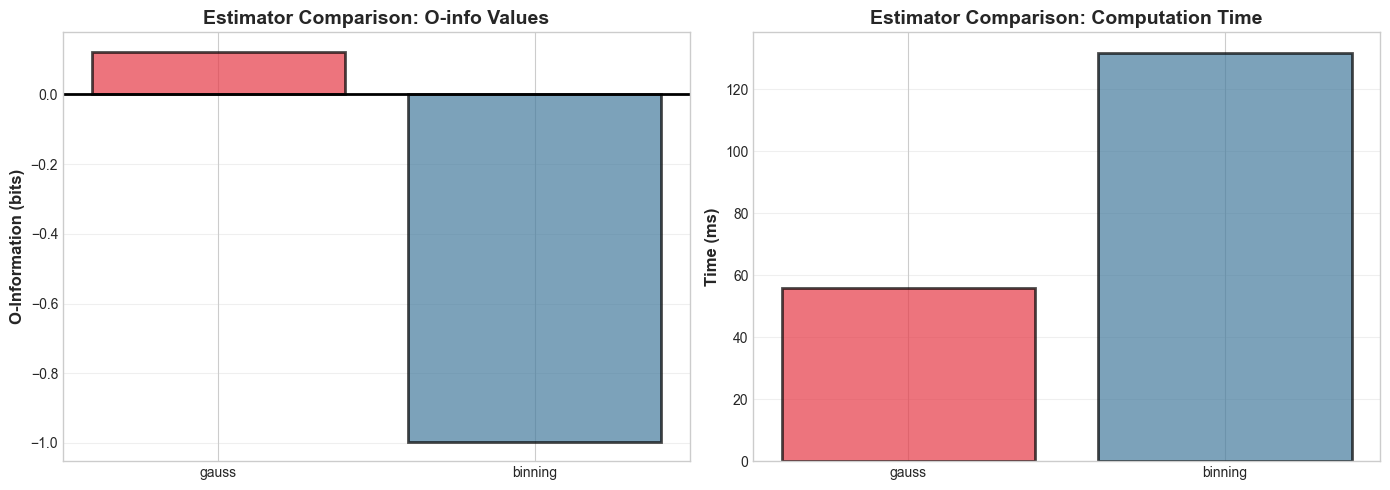
\includegraphics[keepaspectratio]{03_hoi_higher_order_interactions_files/figure-pdf/cell-8-output-4.png}}

\section{Part 4: Partial Information Decomposition
(PID)}\label{part-4-partial-information-decomposition-pid}

\subsection{From O-Information to Detailed
Decomposition}\label{from-o-information-to-detailed-decomposition}

O-information gives us a single number: synergy vs redundancy. But real
systems have \textbf{both}! Partial Information Decomposition (PID)
breaks down the total mutual information into four interpretable
components.

\subsection{The Four PID Atoms}\label{the-four-pid-atoms}

For two source variables \(X_1, X_2\) predicting target \(Y\), PID
decomposes:

\[I(X_1, X_2; Y) = \text{Unique}(X_1) + \text{Unique}(X_2) + \text{Redundancy} + \text{Synergy}\]

Where: - \textbf{Unique(\(X_1\))}: Information in \(X_1\) alone, not in
\(X_2\) - \textbf{Unique(\(X_2\))}: Information in \(X_2\) alone, not in
\(X_1\) - \textbf{Redundancy}: Information carried by \textbf{both}
\(X_1\) and \(X_2\) independently - \textbf{Synergy}: Information that
requires \textbf{both} \(X_1\) and \(X_2\) together

\subsection{Important Note About PID}\label{important-note-about-pid}

PID is uniquely defined for 2 sources but becomes ambiguous for 3+
sources. Different PID measures exist: - \textbf{Williams-Beer}: Minimum
mutual information approach - \textbf{BROJA}: Game-theoretic formulation
- \textbf{MMI (Minimum Mutual Information)}: What HOI implements

They all agree on XOR and COPY (the extremes) but may differ on
intermediate cases.

Let's compute PID for our XOR and COPY examples:

\begin{Shaded}
\begin{Highlighting}[]
\CommentTok{\# HOI implements PID through redundancy and synergy metrics}
\CommentTok{\# The PID classes need x (sources) and y (target) as SEPARATE arguments}

\KeywordTok{def}\NormalTok{ compute\_pid\_atoms(data):}
    \CommentTok{"""}
\CommentTok{    Compute all four PID atoms for data with shape (n\_samples, 3).}
\CommentTok{    Assumes data[:, 0] = X1, data[:, 1] = X2, data[:, 2] = Y}
\CommentTok{    }
\CommentTok{    Parameters:}
\CommentTok{    {-}{-}{-}{-}{-}{-}{-}{-}{-}{-}{-}}
\CommentTok{    data : array of shape (n\_samples, 3)}
\CommentTok{        The three variables stacked column{-}wise}
\CommentTok{    }
\CommentTok{    Returns:}
\CommentTok{    {-}{-}{-}{-}{-}{-}{-}{-}}
\CommentTok{    dict with PID atoms and intermediate values}
\CommentTok{    """}
    \CommentTok{\# Extract sources (X1, X2) and target (Y)}
    \CommentTok{\# x should be (n\_samples, n\_sources) = (n\_samples, 2)}
    \CommentTok{\# y should be (n\_samples,) or (n\_samples, 1)}
\NormalTok{    x }\OperatorTok{=}\NormalTok{ data[:, :}\DecValTok{2}\NormalTok{]  }\CommentTok{\# Sources: X1 and X2}
\NormalTok{    y }\OperatorTok{=}\NormalTok{ data[:, }\DecValTok{2}\NormalTok{]   }\CommentTok{\# Target: Y}
    
    \CommentTok{\# Initialize models with BOTH x and y}
\NormalTok{    model\_red }\OperatorTok{=}\NormalTok{ RedundancyMMI(x, y)}
\NormalTok{    model\_syn }\OperatorTok{=}\NormalTok{ SynergyMMI(x, y)}
    
    \CommentTok{\# Compute redundancy and synergy}
\NormalTok{    redundancy }\OperatorTok{=} \BuiltInTok{float}\NormalTok{(model\_red.fit(method}\OperatorTok{=}\StringTok{\textquotesingle{}binning\textquotesingle{}}\NormalTok{)[}\DecValTok{0}\NormalTok{])}
\NormalTok{    synergy }\OperatorTok{=} \BuiltInTok{float}\NormalTok{(model\_syn.fit(method}\OperatorTok{=}\StringTok{\textquotesingle{}binning\textquotesingle{}}\NormalTok{)[}\DecValTok{0}\NormalTok{])}
    
    \CommentTok{\# For individual mutual informations, we compute them directly}
    \CommentTok{\# I(X1; Y) }
\NormalTok{    x1\_y\_data }\OperatorTok{=}\NormalTok{ np.column\_stack([data[:, }\DecValTok{0}\NormalTok{], data[:, }\DecValTok{2}\NormalTok{]])}
\NormalTok{    model\_mi1 }\OperatorTok{=}\NormalTok{ Oinfo(x1\_y\_data)}
    \CommentTok{\# For 2 variables, TC = MI, so we can use that}
\NormalTok{    tc\_x1\_y }\OperatorTok{=}\NormalTok{ TC(x1\_y\_data)}
\NormalTok{    mi\_x1\_y }\OperatorTok{=} \BuiltInTok{float}\NormalTok{(tc\_x1\_y.fit(method}\OperatorTok{=}\StringTok{\textquotesingle{}binning\textquotesingle{}}\NormalTok{)[}\DecValTok{0}\NormalTok{])}
    
    \CommentTok{\# I(X2; Y)}
\NormalTok{    x2\_y\_data }\OperatorTok{=}\NormalTok{ np.column\_stack([data[:, }\DecValTok{1}\NormalTok{], data[:, }\DecValTok{2}\NormalTok{]])}
\NormalTok{    tc\_x2\_y }\OperatorTok{=}\NormalTok{ TC(x2\_y\_data)}
\NormalTok{    mi\_x2\_y }\OperatorTok{=} \BuiltInTok{float}\NormalTok{(tc\_x2\_y.fit(method}\OperatorTok{=}\StringTok{\textquotesingle{}binning\textquotesingle{}}\NormalTok{)[}\DecValTok{0}\NormalTok{])}
    
    \CommentTok{\# Calculate unique informations}
    \CommentTok{\# Unique(X1) = I(X1; Y) {-} Redundancy (bounded at 0)}
\NormalTok{    unique\_x1 }\OperatorTok{=} \BuiltInTok{max}\NormalTok{(}\DecValTok{0}\NormalTok{, mi\_x1\_y }\OperatorTok{{-}}\NormalTok{ redundancy)}
\NormalTok{    unique\_x2 }\OperatorTok{=} \BuiltInTok{max}\NormalTok{(}\DecValTok{0}\NormalTok{, mi\_x2\_y }\OperatorTok{{-}}\NormalTok{ redundancy)}
    
    \CommentTok{\# Total = Unique1 + Unique2 + Redundancy + Synergy}
\NormalTok{    total }\OperatorTok{=}\NormalTok{ unique\_x1 }\OperatorTok{+}\NormalTok{ unique\_x2 }\OperatorTok{+}\NormalTok{ redundancy }\OperatorTok{+}\NormalTok{ synergy}
    
    \ControlFlowTok{return}\NormalTok{ \{}
        \StringTok{\textquotesingle{}unique\_x1\textquotesingle{}}\NormalTok{: unique\_x1,}
        \StringTok{\textquotesingle{}unique\_x2\textquotesingle{}}\NormalTok{: unique\_x2,}
        \StringTok{\textquotesingle{}redundancy\textquotesingle{}}\NormalTok{: redundancy,}
        \StringTok{\textquotesingle{}synergy\textquotesingle{}}\NormalTok{: synergy,}
        \StringTok{\textquotesingle{}total\textquotesingle{}}\NormalTok{: total,}
        \StringTok{\textquotesingle{}mi\_x1\_y\textquotesingle{}}\NormalTok{: mi\_x1\_y,}
        \StringTok{\textquotesingle{}mi\_x2\_y\textquotesingle{}}\NormalTok{: mi\_x2\_y}
\NormalTok{    \}}

\CommentTok{\# Compute PID for XOR}
\BuiltInTok{print}\NormalTok{(}\StringTok{"PID Decomposition: XOR System"}\NormalTok{)}
\BuiltInTok{print}\NormalTok{(}\StringTok{"="} \OperatorTok{*} \DecValTok{60}\NormalTok{)}
\NormalTok{pid\_xor }\OperatorTok{=}\NormalTok{ compute\_pid\_atoms(data\_xor)}

\BuiltInTok{print}\NormalTok{(}\StringTok{"}\CharTok{\textbackslash{}n}\StringTok{Individual Mutual Informations:"}\NormalTok{)}
\BuiltInTok{print}\NormalTok{(}\SpecialStringTok{f"  I(X₁; Y) = }\SpecialCharTok{\{}\NormalTok{pid\_xor[}\StringTok{\textquotesingle{}mi\_x1\_y\textquotesingle{}}\NormalTok{]}\SpecialCharTok{:.4f\}}\SpecialStringTok{ bits"}\NormalTok{)}
\BuiltInTok{print}\NormalTok{(}\SpecialStringTok{f"  I(X₂; Y) = }\SpecialCharTok{\{}\NormalTok{pid\_xor[}\StringTok{\textquotesingle{}mi\_x2\_y\textquotesingle{}}\NormalTok{]}\SpecialCharTok{:.4f\}}\SpecialStringTok{ bits"}\NormalTok{)}
\BuiltInTok{print}\NormalTok{(}\SpecialStringTok{f"  I(X₁,X₂; Y) ≈ }\SpecialCharTok{\{}\NormalTok{pid\_xor[}\StringTok{\textquotesingle{}total\textquotesingle{}}\NormalTok{]}\SpecialCharTok{:.4f\}}\SpecialStringTok{ bits (from PID sum)"}\NormalTok{)}

\BuiltInTok{print}\NormalTok{(}\StringTok{"}\CharTok{\textbackslash{}n}\StringTok{PID Atoms:"}\NormalTok{)}
\BuiltInTok{print}\NormalTok{(}\SpecialStringTok{f"  Unique(X₁):  }\SpecialCharTok{\{}\NormalTok{pid\_xor[}\StringTok{\textquotesingle{}unique\_x1\textquotesingle{}}\NormalTok{]}\SpecialCharTok{:.4f\}}\SpecialStringTok{ bits"}\NormalTok{)}
\BuiltInTok{print}\NormalTok{(}\SpecialStringTok{f"  Unique(X₂):  }\SpecialCharTok{\{}\NormalTok{pid\_xor[}\StringTok{\textquotesingle{}unique\_x2\textquotesingle{}}\NormalTok{]}\SpecialCharTok{:.4f\}}\SpecialStringTok{ bits"}\NormalTok{)}
\BuiltInTok{print}\NormalTok{(}\SpecialStringTok{f"  Redundancy:  }\SpecialCharTok{\{}\NormalTok{pid\_xor[}\StringTok{\textquotesingle{}redundancy\textquotesingle{}}\NormalTok{]}\SpecialCharTok{:.4f\}}\SpecialStringTok{ bits"}\NormalTok{)}
\BuiltInTok{print}\NormalTok{(}\SpecialStringTok{f"  Synergy:     }\SpecialCharTok{\{}\NormalTok{pid\_xor[}\StringTok{\textquotesingle{}synergy\textquotesingle{}}\NormalTok{]}\SpecialCharTok{:.4f\}}\SpecialStringTok{ bits"}\NormalTok{)}

\BuiltInTok{print}\NormalTok{(}\StringTok{"}\CharTok{\textbackslash{}n}\StringTok{✨ Analysis:"}\NormalTok{)}
\BuiltInTok{print}\NormalTok{(}\StringTok{"  For XOR, synergy should dominate!"}\NormalTok{)}
\BuiltInTok{print}\NormalTok{(}\StringTok{"  Neither X₁ nor X₂ alone provides information about Y,"}\NormalTok{)}
\BuiltInTok{print}\NormalTok{(}\StringTok{"  so unique informations should be \textasciitilde{}0."}\NormalTok{)}
\BuiltInTok{print}\NormalTok{(}\StringTok{"  All information comes from knowing BOTH inputs together."}\NormalTok{)}

\CommentTok{\# Visualize PID}
\NormalTok{fig, ax }\OperatorTok{=}\NormalTok{ plt.subplots(figsize}\OperatorTok{=}\NormalTok{(}\DecValTok{10}\NormalTok{, }\DecValTok{6}\NormalTok{))}
\NormalTok{atoms }\OperatorTok{=}\NormalTok{ [}\StringTok{\textquotesingle{}Unique(X₁)\textquotesingle{}}\NormalTok{, }\StringTok{\textquotesingle{}Unique(X₂)\textquotesingle{}}\NormalTok{, }\StringTok{\textquotesingle{}Redundancy\textquotesingle{}}\NormalTok{, }\StringTok{\textquotesingle{}Synergy\textquotesingle{}}\NormalTok{]}
\NormalTok{values }\OperatorTok{=}\NormalTok{ [pid\_xor[}\StringTok{\textquotesingle{}unique\_x1\textquotesingle{}}\NormalTok{], pid\_xor[}\StringTok{\textquotesingle{}unique\_x2\textquotesingle{}}\NormalTok{], pid\_xor[}\StringTok{\textquotesingle{}redundancy\textquotesingle{}}\NormalTok{], pid\_xor[}\StringTok{\textquotesingle{}synergy\textquotesingle{}}\NormalTok{]]}
\NormalTok{colors }\OperatorTok{=}\NormalTok{ [}\StringTok{\textquotesingle{}\#E63946\textquotesingle{}}\NormalTok{, }\StringTok{\textquotesingle{}\#F1FAEE\textquotesingle{}}\NormalTok{, }\StringTok{\textquotesingle{}\#457B9D\textquotesingle{}}\NormalTok{, }\StringTok{\textquotesingle{}\#A8DADC\textquotesingle{}}\NormalTok{]}

\NormalTok{bars }\OperatorTok{=}\NormalTok{ ax.bar(atoms, values, color}\OperatorTok{=}\NormalTok{colors, alpha}\OperatorTok{=}\FloatTok{0.8}\NormalTok{, edgecolor}\OperatorTok{=}\StringTok{\textquotesingle{}black\textquotesingle{}}\NormalTok{, linewidth}\OperatorTok{=}\DecValTok{2}\NormalTok{)}
\NormalTok{ax.set\_ylabel(}\StringTok{\textquotesingle{}Information (bits)\textquotesingle{}}\NormalTok{, fontsize}\OperatorTok{=}\DecValTok{14}\NormalTok{, fontweight}\OperatorTok{=}\StringTok{\textquotesingle{}bold\textquotesingle{}}\NormalTok{)}
\NormalTok{ax.set\_title(}\StringTok{\textquotesingle{}PID Decomposition of XOR System\textquotesingle{}}\NormalTok{, fontsize}\OperatorTok{=}\DecValTok{16}\NormalTok{, fontweight}\OperatorTok{=}\StringTok{\textquotesingle{}bold\textquotesingle{}}\NormalTok{)}
\NormalTok{ax.grid(}\VariableTok{True}\NormalTok{, alpha}\OperatorTok{=}\FloatTok{0.3}\NormalTok{, axis}\OperatorTok{=}\StringTok{\textquotesingle{}y\textquotesingle{}}\NormalTok{)}

\ControlFlowTok{for}\NormalTok{ bar, val }\KeywordTok{in} \BuiltInTok{zip}\NormalTok{(bars, values):}
\NormalTok{    ax.text(bar.get\_x() }\OperatorTok{+}\NormalTok{ bar.get\_width()}\OperatorTok{/}\DecValTok{2}\NormalTok{, bar.get\_height() }\OperatorTok{+} \FloatTok{0.02}\NormalTok{, }
            \SpecialStringTok{f\textquotesingle{}}\SpecialCharTok{\{}\NormalTok{val}\SpecialCharTok{:.3f\}}\SpecialStringTok{\textquotesingle{}}\NormalTok{, ha}\OperatorTok{=}\StringTok{\textquotesingle{}center\textquotesingle{}}\NormalTok{, fontweight}\OperatorTok{=}\StringTok{\textquotesingle{}bold\textquotesingle{}}\NormalTok{, fontsize}\OperatorTok{=}\DecValTok{11}\NormalTok{)}

\NormalTok{plt.tight\_layout()}
\NormalTok{plt.show()}
\end{Highlighting}
\end{Shaded}

\begin{verbatim}
PID Decomposition: XOR System
============================================================
\end{verbatim}

\begin{verbatim}

Individual Mutual Informations:
  I(X₁; Y) = 0.0024 bits
  I(X₂; Y) = 0.0006 bits
  I(X₁,X₂; Y) ≈ 0.9993 bits (from PID sum)

PID Atoms:
  Unique(X₁):  0.0018 bits
  Unique(X₂):  0.0000 bits
  Redundancy:  0.0006 bits
  Synergy:     0.9969 bits

✨ Analysis:
  For XOR, synergy should dominate!
  Neither X₁ nor X₂ alone provides information about Y,
  so unique informations should be ~0.
  All information comes from knowing BOTH inputs together.
\end{verbatim}

\pandocbounded{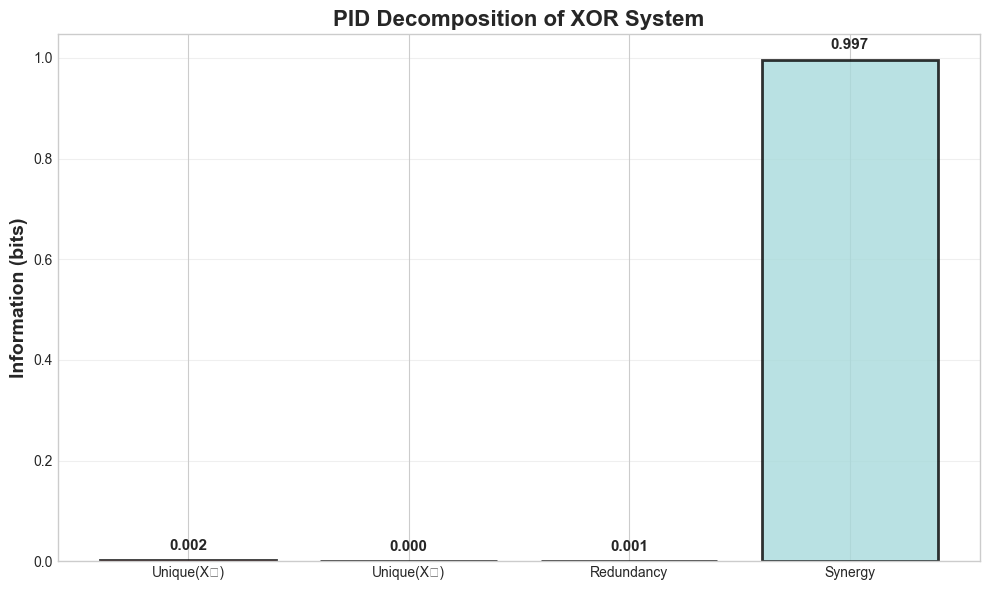
\includegraphics[keepaspectratio]{03_hoi_higher_order_interactions_files/figure-pdf/cell-9-output-3.png}}

\subsection{Visualizing PID Atoms}\label{visualizing-pid-atoms}

Let's create a comprehensive visualization showing how PID decomposes
information for different systems:

\begin{Shaded}
\begin{Highlighting}[]
\CommentTok{\# Compute PID for multiple systems}
\NormalTok{systems\_pid }\OperatorTok{=}\NormalTok{ \{}
    \StringTok{\textquotesingle{}XOR}\CharTok{\textbackslash{}n}\StringTok{(Pure Synergy)\textquotesingle{}}\NormalTok{: data\_xor,}
    \StringTok{\textquotesingle{}COPY}\CharTok{\textbackslash{}n}\StringTok{(Pure Redundancy)\textquotesingle{}}\NormalTok{: data\_copy,}
\NormalTok{\}}

\CommentTok{\# Add AND gate}
\NormalTok{X1\_and }\OperatorTok{=}\NormalTok{ np.random.binomial(}\DecValTok{1}\NormalTok{, }\FloatTok{0.5}\NormalTok{, n\_samples)}
\NormalTok{X2\_and }\OperatorTok{=}\NormalTok{ np.random.binomial(}\DecValTok{1}\NormalTok{, }\FloatTok{0.5}\NormalTok{, n\_samples)}
\NormalTok{Y\_and }\OperatorTok{=}\NormalTok{ np.logical\_and(X1\_and, X2\_and).astype(}\BuiltInTok{float}\NormalTok{)}
\NormalTok{systems\_pid[}\StringTok{\textquotesingle{}AND}\CharTok{\textbackslash{}n}\StringTok{(Mixed)\textquotesingle{}}\NormalTok{] }\OperatorTok{=}\NormalTok{ np.column\_stack([X1\_and, X2\_and, Y\_and])}

\CommentTok{\# Compute PID for all}
\NormalTok{pid\_results }\OperatorTok{=}\NormalTok{ \{\}}
\ControlFlowTok{for}\NormalTok{ name, data }\KeywordTok{in}\NormalTok{ systems\_pid.items():}
    \ControlFlowTok{try}\NormalTok{:}
\NormalTok{        pid\_results[name] }\OperatorTok{=}\NormalTok{ compute\_pid\_atoms(data)}
        \BuiltInTok{print}\NormalTok{(}\SpecialStringTok{f"✓ Computed PID for }\SpecialCharTok{\{}\NormalTok{name}\SpecialCharTok{.}\NormalTok{replace(}\BuiltInTok{chr}\NormalTok{(}\DecValTok{10}\NormalTok{), }\StringTok{\textquotesingle{} \textquotesingle{}}\NormalTok{)}\SpecialCharTok{\}}\SpecialStringTok{"}\NormalTok{)}
    \ControlFlowTok{except} \PreprocessorTok{Exception} \ImportTok{as}\NormalTok{ e:}
        \BuiltInTok{print}\NormalTok{(}\SpecialStringTok{f"⚠ Warning: Could not compute PID for }\SpecialCharTok{\{}\NormalTok{name}\SpecialCharTok{.}\NormalTok{replace(}\BuiltInTok{chr}\NormalTok{(}\DecValTok{10}\NormalTok{), }\StringTok{\textquotesingle{} \textquotesingle{}}\NormalTok{)}\SpecialCharTok{\}}\SpecialStringTok{: }\SpecialCharTok{\{}\NormalTok{e}\SpecialCharTok{\}}\SpecialStringTok{"}\NormalTok{)}
        \ControlFlowTok{continue}

\ControlFlowTok{if} \BuiltInTok{len}\NormalTok{(pid\_results) }\OperatorTok{\textgreater{}} \DecValTok{0}\NormalTok{:}
    \CommentTok{\# Create stacked bar chart}
\NormalTok{    fig, ax }\OperatorTok{=}\NormalTok{ plt.subplots(}\DecValTok{1}\NormalTok{, }\DecValTok{1}\NormalTok{, figsize}\OperatorTok{=}\NormalTok{(}\DecValTok{14}\NormalTok{, }\DecValTok{8}\NormalTok{))}

\NormalTok{    names }\OperatorTok{=} \BuiltInTok{list}\NormalTok{(pid\_results.keys())}
\NormalTok{    x }\OperatorTok{=}\NormalTok{ np.arange(}\BuiltInTok{len}\NormalTok{(names))}
\NormalTok{    width }\OperatorTok{=} \FloatTok{0.6}

    \CommentTok{\# Extract values for each atom}
\NormalTok{    unique1 }\OperatorTok{=}\NormalTok{ [pid\_results[n][}\StringTok{\textquotesingle{}unique\_x1\textquotesingle{}}\NormalTok{] }\ControlFlowTok{for}\NormalTok{ n }\KeywordTok{in}\NormalTok{ names]}
\NormalTok{    unique2 }\OperatorTok{=}\NormalTok{ [pid\_results[n][}\StringTok{\textquotesingle{}unique\_x2\textquotesingle{}}\NormalTok{] }\ControlFlowTok{for}\NormalTok{ n }\KeywordTok{in}\NormalTok{ names]}
\NormalTok{    redundancy }\OperatorTok{=}\NormalTok{ [pid\_results[n][}\StringTok{\textquotesingle{}redundancy\textquotesingle{}}\NormalTok{] }\ControlFlowTok{for}\NormalTok{ n }\KeywordTok{in}\NormalTok{ names]}
\NormalTok{    synergy }\OperatorTok{=}\NormalTok{ [pid\_results[n][}\StringTok{\textquotesingle{}synergy\textquotesingle{}}\NormalTok{] }\ControlFlowTok{for}\NormalTok{ n }\KeywordTok{in}\NormalTok{ names]}

    \CommentTok{\# Create stacked bars}
\NormalTok{    p1 }\OperatorTok{=}\NormalTok{ ax.bar(x, unique1, width, label}\OperatorTok{=}\StringTok{\textquotesingle{}Unique(X₁)\textquotesingle{}}\NormalTok{, color}\OperatorTok{=}\StringTok{\textquotesingle{}\#E63946\textquotesingle{}}\NormalTok{, alpha}\OperatorTok{=}\FloatTok{0.8}\NormalTok{, edgecolor}\OperatorTok{=}\StringTok{\textquotesingle{}black\textquotesingle{}}\NormalTok{)}
\NormalTok{    p2 }\OperatorTok{=}\NormalTok{ ax.bar(x, unique2, width, bottom}\OperatorTok{=}\NormalTok{unique1, label}\OperatorTok{=}\StringTok{\textquotesingle{}Unique(X₂)\textquotesingle{}}\NormalTok{, color}\OperatorTok{=}\StringTok{\textquotesingle{}\#F1FAEE\textquotesingle{}}\NormalTok{, alpha}\OperatorTok{=}\FloatTok{0.8}\NormalTok{, edgecolor}\OperatorTok{=}\StringTok{\textquotesingle{}black\textquotesingle{}}\NormalTok{)}
\NormalTok{    p3 }\OperatorTok{=}\NormalTok{ ax.bar(x, redundancy, width, bottom}\OperatorTok{=}\NormalTok{np.array(unique1)}\OperatorTok{+}\NormalTok{np.array(unique2), }
\NormalTok{                label}\OperatorTok{=}\StringTok{\textquotesingle{}Redundancy\textquotesingle{}}\NormalTok{, color}\OperatorTok{=}\StringTok{\textquotesingle{}\#457B9D\textquotesingle{}}\NormalTok{, alpha}\OperatorTok{=}\FloatTok{0.8}\NormalTok{, edgecolor}\OperatorTok{=}\StringTok{\textquotesingle{}black\textquotesingle{}}\NormalTok{)}
\NormalTok{    p4 }\OperatorTok{=}\NormalTok{ ax.bar(x, synergy, width, bottom}\OperatorTok{=}\NormalTok{np.array(unique1)}\OperatorTok{+}\NormalTok{np.array(unique2)}\OperatorTok{+}\NormalTok{np.array(redundancy), }
\NormalTok{                label}\OperatorTok{=}\StringTok{\textquotesingle{}Synergy\textquotesingle{}}\NormalTok{, color}\OperatorTok{=}\StringTok{\textquotesingle{}\#A8DADC\textquotesingle{}}\NormalTok{, alpha}\OperatorTok{=}\FloatTok{0.8}\NormalTok{, edgecolor}\OperatorTok{=}\StringTok{\textquotesingle{}black\textquotesingle{}}\NormalTok{)}

    \CommentTok{\# Labels and formatting}
\NormalTok{    ax.set\_ylabel(}\StringTok{\textquotesingle{}Information (bits)\textquotesingle{}}\NormalTok{, fontsize}\OperatorTok{=}\DecValTok{14}\NormalTok{, fontweight}\OperatorTok{=}\StringTok{\textquotesingle{}bold\textquotesingle{}}\NormalTok{)}
\NormalTok{    ax.set\_title(}\StringTok{\textquotesingle{}PID Decomposition Across Systems\textquotesingle{}}\NormalTok{, fontsize}\OperatorTok{=}\DecValTok{16}\NormalTok{, fontweight}\OperatorTok{=}\StringTok{\textquotesingle{}bold\textquotesingle{}}\NormalTok{, pad}\OperatorTok{=}\DecValTok{20}\NormalTok{)}
\NormalTok{    ax.set\_xticks(x)}
\NormalTok{    ax.set\_xticklabels(names, fontsize}\OperatorTok{=}\DecValTok{12}\NormalTok{, fontweight}\OperatorTok{=}\StringTok{\textquotesingle{}bold\textquotesingle{}}\NormalTok{)}
\NormalTok{    ax.legend(fontsize}\OperatorTok{=}\DecValTok{12}\NormalTok{, loc}\OperatorTok{=}\StringTok{\textquotesingle{}upper right\textquotesingle{}}\NormalTok{)}
\NormalTok{    ax.grid(}\VariableTok{True}\NormalTok{, alpha}\OperatorTok{=}\FloatTok{0.3}\NormalTok{, axis}\OperatorTok{=}\StringTok{\textquotesingle{}y\textquotesingle{}}\NormalTok{)}

    \CommentTok{\# Add total information labels}
    \ControlFlowTok{for}\NormalTok{ i, name }\KeywordTok{in} \BuiltInTok{enumerate}\NormalTok{(names):}
\NormalTok{        total }\OperatorTok{=}\NormalTok{ pid\_results[name][}\StringTok{\textquotesingle{}total\textquotesingle{}}\NormalTok{]}
\NormalTok{        ax.text(i, total }\OperatorTok{+} \FloatTok{0.05}\NormalTok{, }\SpecialStringTok{f\textquotesingle{}Total:}\CharTok{\textbackslash{}n}\SpecialCharTok{\{}\NormalTok{total}\SpecialCharTok{:.3f\}}\SpecialStringTok{\textquotesingle{}}\NormalTok{, }
\NormalTok{                ha}\OperatorTok{=}\StringTok{\textquotesingle{}center\textquotesingle{}}\NormalTok{, fontweight}\OperatorTok{=}\StringTok{\textquotesingle{}bold\textquotesingle{}}\NormalTok{, fontsize}\OperatorTok{=}\DecValTok{10}\NormalTok{)}

\NormalTok{    plt.tight\_layout()}
\NormalTok{    plt.show()}

    \CommentTok{\# Print summary table}
    \BuiltInTok{print}\NormalTok{(}\StringTok{"}\CharTok{\textbackslash{}n}\StringTok{PID Summary Table:"}\NormalTok{)}
    \BuiltInTok{print}\NormalTok{(}\StringTok{"="} \OperatorTok{*} \DecValTok{80}\NormalTok{)}
    \BuiltInTok{print}\NormalTok{(}\SpecialStringTok{f"}\SpecialCharTok{\{}\StringTok{\textquotesingle{}System\textquotesingle{}}\SpecialCharTok{:\textless{}25\}}\SpecialStringTok{ }\SpecialCharTok{\{}\StringTok{\textquotesingle{}Unique1\textquotesingle{}}\SpecialCharTok{:\textgreater{}10\}}\SpecialStringTok{ }\SpecialCharTok{\{}\StringTok{\textquotesingle{}Unique2\textquotesingle{}}\SpecialCharTok{:\textgreater{}10\}}\SpecialStringTok{ }\SpecialCharTok{\{}\StringTok{\textquotesingle{}Redund\textquotesingle{}}\SpecialCharTok{:\textgreater{}10\}}\SpecialStringTok{ }\SpecialCharTok{\{}\StringTok{\textquotesingle{}Synergy\textquotesingle{}}\SpecialCharTok{:\textgreater{}10\}}\SpecialStringTok{ }\SpecialCharTok{\{}\StringTok{\textquotesingle{}Total\textquotesingle{}}\SpecialCharTok{:\textgreater{}10\}}\SpecialStringTok{"}\NormalTok{)}
    \BuiltInTok{print}\NormalTok{(}\StringTok{"="} \OperatorTok{*} \DecValTok{80}\NormalTok{)}
    \ControlFlowTok{for}\NormalTok{ name }\KeywordTok{in}\NormalTok{ names:}
\NormalTok{        p }\OperatorTok{=}\NormalTok{ pid\_results[name]}
\NormalTok{        name\_clean }\OperatorTok{=}\NormalTok{ name.replace(}\StringTok{\textquotesingle{}}\CharTok{\textbackslash{}n}\StringTok{\textquotesingle{}}\NormalTok{, }\StringTok{\textquotesingle{} \textquotesingle{}}\NormalTok{)}
        \BuiltInTok{print}\NormalTok{(}\SpecialStringTok{f"}\SpecialCharTok{\{}\NormalTok{name\_clean}\SpecialCharTok{:\textless{}25\}}\SpecialStringTok{ }\SpecialCharTok{\{}\NormalTok{p[}\StringTok{\textquotesingle{}unique\_x1\textquotesingle{}}\NormalTok{]}\SpecialCharTok{:\textgreater{}10.4f\}}\SpecialStringTok{ }\SpecialCharTok{\{}\NormalTok{p[}\StringTok{\textquotesingle{}unique\_x2\textquotesingle{}}\NormalTok{]}\SpecialCharTok{:\textgreater{}10.4f\}}\SpecialStringTok{ "}
              \SpecialStringTok{f"}\SpecialCharTok{\{}\NormalTok{p[}\StringTok{\textquotesingle{}redundancy\textquotesingle{}}\NormalTok{]}\SpecialCharTok{:\textgreater{}10.4f\}}\SpecialStringTok{ }\SpecialCharTok{\{}\NormalTok{p[}\StringTok{\textquotesingle{}synergy\textquotesingle{}}\NormalTok{]}\SpecialCharTok{:\textgreater{}10.4f\}}\SpecialStringTok{ }\SpecialCharTok{\{}\NormalTok{p[}\StringTok{\textquotesingle{}total\textquotesingle{}}\NormalTok{]}\SpecialCharTok{:\textgreater{}10.4f\}}\SpecialStringTok{"}\NormalTok{)}
\end{Highlighting}
\end{Shaded}

\begin{verbatim}
✓ Computed PID for XOR (Pure Synergy)
\end{verbatim}

\begin{verbatim}
✓ Computed PID for COPY (Pure Redundancy)
⚠ Warning: Could not compute PID for AND (Mixed): data dtype should be integer. Check that you discretized your data. If so, use `data.astype(int)`
\end{verbatim}

\pandocbounded{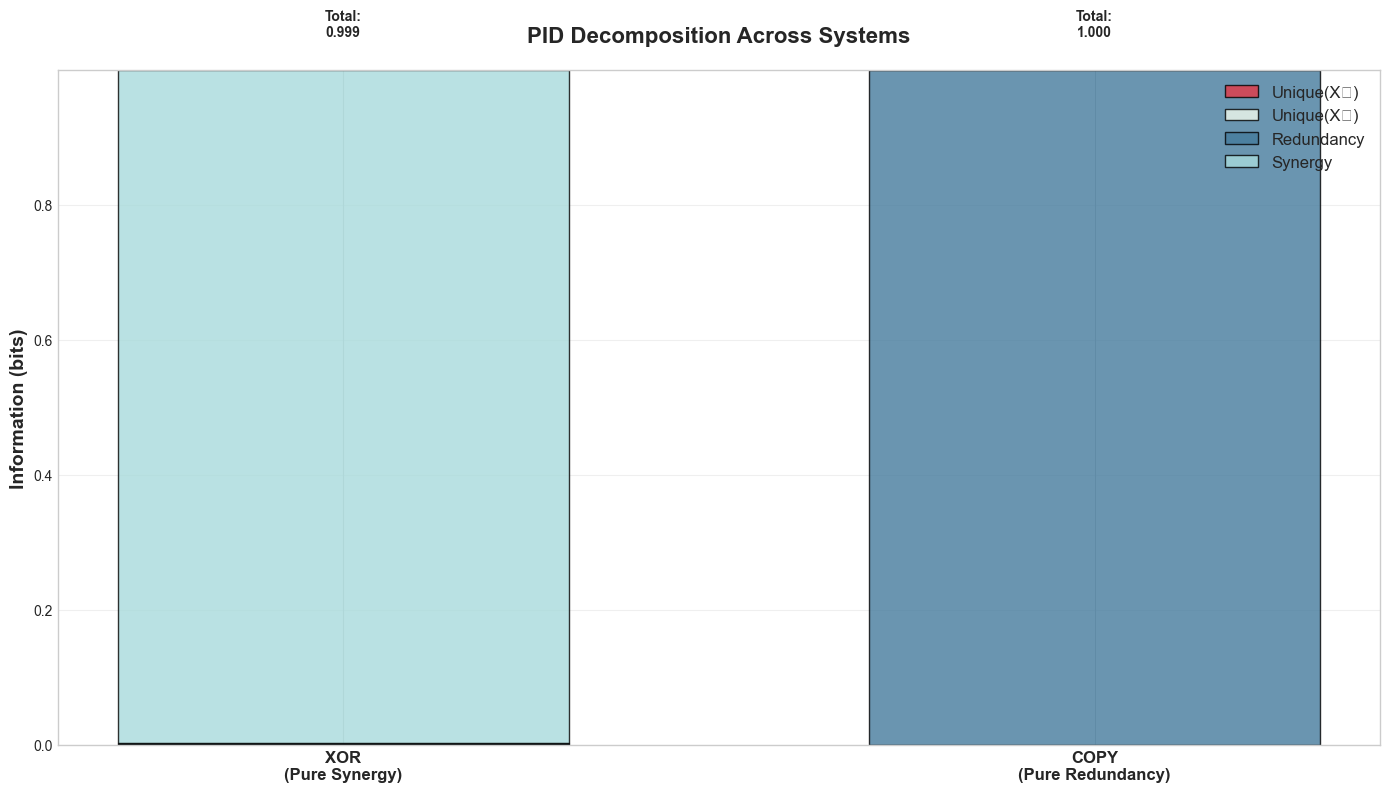
\includegraphics[keepaspectratio]{03_hoi_higher_order_interactions_files/figure-pdf/cell-10-output-3.png}}

\begin{verbatim}

PID Summary Table:
================================================================================
System                       Unique1    Unique2     Redund    Synergy      Total
================================================================================
XOR (Pure Synergy)            0.0018     0.0000     0.0006     0.9969     0.9993
COPY (Pure Redundancy)        0.0000     0.0000     0.9997     0.0000     0.9997
\end{verbatim}

\section{Part 5: Application to Simulated Neural
Data}\label{part-5-application-to-simulated-neural-data}

\subsection{Realistic Neural Population
Scenario}\label{realistic-neural-population-scenario}

Now let's apply everything we've learned to a more realistic
neuroscience scenario. We'll simulate a small population of V1 neurons
encoding visual orientation, then use HOI to discover their information
structure.

\textbf{Scenario}: - 10 V1 neurons - 8 orientations (0°, 45°, 90°, 135°,
180°, 225°, 270°, 315°) - 500 trials - Each neuron has a preferred
orientation - Some neurons encode independently - Some form synergistic
pairs - Some are redundant (overlapping tuning)

This mimics real V1 organization where neurons with similar orientation
preferences cluster together (orientation columns).

\begin{Shaded}
\begin{Highlighting}[]
\KeywordTok{def}\NormalTok{ generate\_v1\_population(n\_neurons}\OperatorTok{=}\DecValTok{10}\NormalTok{, n\_trials}\OperatorTok{=}\DecValTok{500}\NormalTok{, n\_orientations}\OperatorTok{=}\DecValTok{8}\NormalTok{, seed}\OperatorTok{=}\DecValTok{42}\NormalTok{):}
    \CommentTok{"""}
\CommentTok{    Generate realistic V1 population responses with mixed information structure.}
\CommentTok{    }
\CommentTok{    Returns:}
\CommentTok{    {-}{-}{-}{-}{-}{-}{-}{-}}
\CommentTok{    responses : array (n\_neurons, n\_trials)}
\CommentTok{        Neural responses (spike counts)}
\CommentTok{    orientations : array (n\_trials,)}
\CommentTok{        Stimulus orientation for each trial}
\CommentTok{    neuron\_props : dict}
\CommentTok{        Properties of each neuron (preferred orientation, tuning width, etc.)}
\CommentTok{    """}
\NormalTok{    np.random.seed(seed)}
    
    \CommentTok{\# Stimulus orientations}
\NormalTok{    ori\_values }\OperatorTok{=}\NormalTok{ np.linspace(}\DecValTok{0}\NormalTok{, }\DecValTok{360}\NormalTok{, n\_orientations, endpoint}\OperatorTok{=}\VariableTok{False}\NormalTok{)}
\NormalTok{    trial\_oris }\OperatorTok{=}\NormalTok{ np.random.choice(ori\_values, n\_trials)}
    
    \CommentTok{\# Initialize responses}
\NormalTok{    responses }\OperatorTok{=}\NormalTok{ np.zeros((n\_neurons, n\_trials))}
\NormalTok{    neuron\_props }\OperatorTok{=}\NormalTok{ []}
    
    \ControlFlowTok{for}\NormalTok{ i }\KeywordTok{in} \BuiltInTok{range}\NormalTok{(n\_neurons):}
        \CommentTok{\# Each neuron\textquotesingle{}s parameters}
\NormalTok{        pref\_ori }\OperatorTok{=}\NormalTok{ (i }\OperatorTok{*} \DecValTok{360} \OperatorTok{/}\NormalTok{ n\_neurons) }\OperatorTok{+}\NormalTok{ np.random.randn() }\OperatorTok{*} \DecValTok{10}  \CommentTok{\# Slight jitter}
\NormalTok{        tuning\_width }\OperatorTok{=} \DecValTok{30} \OperatorTok{+}\NormalTok{ np.random.rand() }\OperatorTok{*} \DecValTok{30}  \CommentTok{\# 30{-}60 degrees}
\NormalTok{        max\_rate }\OperatorTok{=} \DecValTok{40} \OperatorTok{+}\NormalTok{ np.random.rand() }\OperatorTok{*} \DecValTok{40}  \CommentTok{\# 40{-}80 Hz}
\NormalTok{        baseline }\OperatorTok{=} \DecValTok{5} \OperatorTok{+}\NormalTok{ np.random.rand() }\OperatorTok{*} \DecValTok{10}  \CommentTok{\# 5{-}15 Hz}
\NormalTok{        noise\_level }\OperatorTok{=} \FloatTok{0.3} \OperatorTok{+}\NormalTok{ np.random.rand() }\OperatorTok{*} \FloatTok{0.4}  \CommentTok{\# Variable noise}
        
\NormalTok{        neuron\_props.append(\{}
            \StringTok{\textquotesingle{}id\textquotesingle{}}\NormalTok{: i,}
            \StringTok{\textquotesingle{}pref\_ori\textquotesingle{}}\NormalTok{: pref\_ori,}
            \StringTok{\textquotesingle{}tuning\_width\textquotesingle{}}\NormalTok{: tuning\_width,}
            \StringTok{\textquotesingle{}max\_rate\textquotesingle{}}\NormalTok{: max\_rate,}
            \StringTok{\textquotesingle{}baseline\textquotesingle{}}\NormalTok{: baseline}
\NormalTok{        \})}
        
        \CommentTok{\# Generate responses}
        \ControlFlowTok{for}\NormalTok{ j, ori }\KeywordTok{in} \BuiltInTok{enumerate}\NormalTok{(trial\_oris):}
            \CommentTok{\# Angular distance}
\NormalTok{            dist }\OperatorTok{=} \BuiltInTok{min}\NormalTok{(}\BuiltInTok{abs}\NormalTok{(ori }\OperatorTok{{-}}\NormalTok{ pref\_ori), }\DecValTok{360} \OperatorTok{{-}} \BuiltInTok{abs}\NormalTok{(ori }\OperatorTok{{-}}\NormalTok{ pref\_ori))}
            
            \CommentTok{\# Von Mises tuning}
\NormalTok{            tuning }\OperatorTok{=}\NormalTok{ np.exp(}\OperatorTok{{-}}\NormalTok{(dist}\OperatorTok{**}\DecValTok{2}\NormalTok{) }\OperatorTok{/}\NormalTok{ (}\DecValTok{2} \OperatorTok{*}\NormalTok{ tuning\_width}\OperatorTok{**}\DecValTok{2}\NormalTok{))}
\NormalTok{            mean\_rate }\OperatorTok{=}\NormalTok{ baseline }\OperatorTok{+}\NormalTok{ (max\_rate }\OperatorTok{{-}}\NormalTok{ baseline) }\OperatorTok{*}\NormalTok{ tuning}
            
            \CommentTok{\# Poisson variability}
\NormalTok{            responses[i, j] }\OperatorTok{=}\NormalTok{ np.random.poisson(mean\_rate)}
    
    \ControlFlowTok{return}\NormalTok{ responses, trial\_oris, neuron\_props}

\CommentTok{\# Generate population}
\NormalTok{responses, orientations, neuron\_props }\OperatorTok{=}\NormalTok{ generate\_v1\_population()}

\BuiltInTok{print}\NormalTok{(}\StringTok{"V1 Population Generated"}\NormalTok{)}
\BuiltInTok{print}\NormalTok{(}\StringTok{"="} \OperatorTok{*} \DecValTok{60}\NormalTok{)}
\BuiltInTok{print}\NormalTok{(}\SpecialStringTok{f"Shape: }\SpecialCharTok{\{}\NormalTok{responses}\SpecialCharTok{.}\NormalTok{shape}\SpecialCharTok{\}}\SpecialStringTok{ (neurons × trials)"}\NormalTok{)}
\BuiltInTok{print}\NormalTok{(}\SpecialStringTok{f"Orientation values: }\SpecialCharTok{\{}\NormalTok{np}\SpecialCharTok{.}\NormalTok{unique(orientations)}\SpecialCharTok{\}}\SpecialStringTok{°"}\NormalTok{)}
\BuiltInTok{print}\NormalTok{(}\SpecialStringTok{f"}\CharTok{\textbackslash{}n}\SpecialStringTok{Neuron properties (first 3):"}\NormalTok{)}
\ControlFlowTok{for}\NormalTok{ i }\KeywordTok{in} \BuiltInTok{range}\NormalTok{(}\DecValTok{3}\NormalTok{):}
\NormalTok{    prop }\OperatorTok{=}\NormalTok{ neuron\_props[i]}
    \BuiltInTok{print}\NormalTok{(}\SpecialStringTok{f"  Neuron }\SpecialCharTok{\{}\NormalTok{i}\SpecialCharTok{\}}\SpecialStringTok{: pref=}\SpecialCharTok{\{}\NormalTok{prop[}\StringTok{\textquotesingle{}pref\_ori\textquotesingle{}}\NormalTok{]}\SpecialCharTok{:.1f\}}\SpecialStringTok{°, "}
          \SpecialStringTok{f"width=}\SpecialCharTok{\{}\NormalTok{prop[}\StringTok{\textquotesingle{}tuning\_width\textquotesingle{}}\NormalTok{]}\SpecialCharTok{:.1f\}}\SpecialStringTok{°, max=}\SpecialCharTok{\{}\NormalTok{prop[}\StringTok{\textquotesingle{}max\_rate\textquotesingle{}}\NormalTok{]}\SpecialCharTok{:.1f\}}\SpecialStringTok{Hz"}\NormalTok{)}

\CommentTok{\# Visualize tuning curves}
\NormalTok{fig, axes }\OperatorTok{=}\NormalTok{ plt.subplots(}\DecValTok{2}\NormalTok{, }\DecValTok{5}\NormalTok{, figsize}\OperatorTok{=}\NormalTok{(}\DecValTok{18}\NormalTok{, }\DecValTok{8}\NormalTok{))}
\NormalTok{axes }\OperatorTok{=}\NormalTok{ axes.flatten()}

\NormalTok{ori\_vals }\OperatorTok{=}\NormalTok{ np.unique(orientations)}
\ControlFlowTok{for}\NormalTok{ i }\KeywordTok{in} \BuiltInTok{range}\NormalTok{(}\DecValTok{10}\NormalTok{):}
\NormalTok{    ax }\OperatorTok{=}\NormalTok{ axes[i]}
    
    \CommentTok{\# Compute mean response for each orientation}
\NormalTok{    mean\_responses }\OperatorTok{=}\NormalTok{ []}
    \ControlFlowTok{for}\NormalTok{ ori }\KeywordTok{in}\NormalTok{ ori\_vals:}
\NormalTok{        trials\_this\_ori }\OperatorTok{=}\NormalTok{ orientations }\OperatorTok{==}\NormalTok{ ori}
\NormalTok{        mean\_resp }\OperatorTok{=}\NormalTok{ responses[i, trials\_this\_ori].mean()}
\NormalTok{        mean\_responses.append(mean\_resp)}
    
    \CommentTok{\# Plot}
\NormalTok{    ax.plot(ori\_vals, mean\_responses, }\StringTok{\textquotesingle{}o{-}\textquotesingle{}}\NormalTok{, linewidth}\OperatorTok{=}\DecValTok{2}\NormalTok{, markersize}\OperatorTok{=}\DecValTok{8}\NormalTok{)}
\NormalTok{    ax.set\_xlabel(}\StringTok{\textquotesingle{}Orientation (°)\textquotesingle{}}\NormalTok{, fontsize}\OperatorTok{=}\DecValTok{10}\NormalTok{)}
\NormalTok{    ax.set\_ylabel(}\StringTok{\textquotesingle{}Firing Rate (Hz)\textquotesingle{}}\NormalTok{, fontsize}\OperatorTok{=}\DecValTok{10}\NormalTok{)}
\NormalTok{    ax.set\_title(}\SpecialStringTok{f\textquotesingle{}Neuron }\SpecialCharTok{\{}\NormalTok{i}\SpecialCharTok{\}}\SpecialStringTok{\textquotesingle{}}\NormalTok{, fontsize}\OperatorTok{=}\DecValTok{11}\NormalTok{, fontweight}\OperatorTok{=}\StringTok{\textquotesingle{}bold\textquotesingle{}}\NormalTok{)}
\NormalTok{    ax.grid(}\VariableTok{True}\NormalTok{, alpha}\OperatorTok{=}\FloatTok{0.3}\NormalTok{)}
\NormalTok{    ax.set\_xticks([}\DecValTok{0}\NormalTok{, }\DecValTok{90}\NormalTok{, }\DecValTok{180}\NormalTok{, }\DecValTok{270}\NormalTok{])}

\NormalTok{plt.suptitle(}\StringTok{\textquotesingle{}V1 Population Tuning Curves\textquotesingle{}}\NormalTok{, fontsize}\OperatorTok{=}\DecValTok{16}\NormalTok{, fontweight}\OperatorTok{=}\StringTok{\textquotesingle{}bold\textquotesingle{}}\NormalTok{, y}\OperatorTok{=}\FloatTok{1.02}\NormalTok{)}
\NormalTok{plt.tight\_layout()}
\NormalTok{plt.show()}

\BuiltInTok{print}\NormalTok{(}\StringTok{"}\CharTok{\textbackslash{}n}\StringTok{✓ Population exhibits realistic orientation selectivity"}\NormalTok{)}
\BuiltInTok{print}\NormalTok{(}\StringTok{"  Now let\textquotesingle{}s discover the information structure..."}\NormalTok{)}
\end{Highlighting}
\end{Shaded}

\begin{verbatim}
V1 Population Generated
============================================================
Shape: (10, 500) (neurons × trials)
Orientation values: [  0.  45.  90. 135. 180. 225. 270. 315.]°

Neuron properties (first 3):
  Neuron 0: pref=-8.5°, width=55.5°, max=52.7Hz
  Neuron 1: pref=20.9°, width=30.2°, max=48.8Hz
  Neuron 2: pref=65.7°, width=32.0°, max=52.7Hz
\end{verbatim}

\pandocbounded{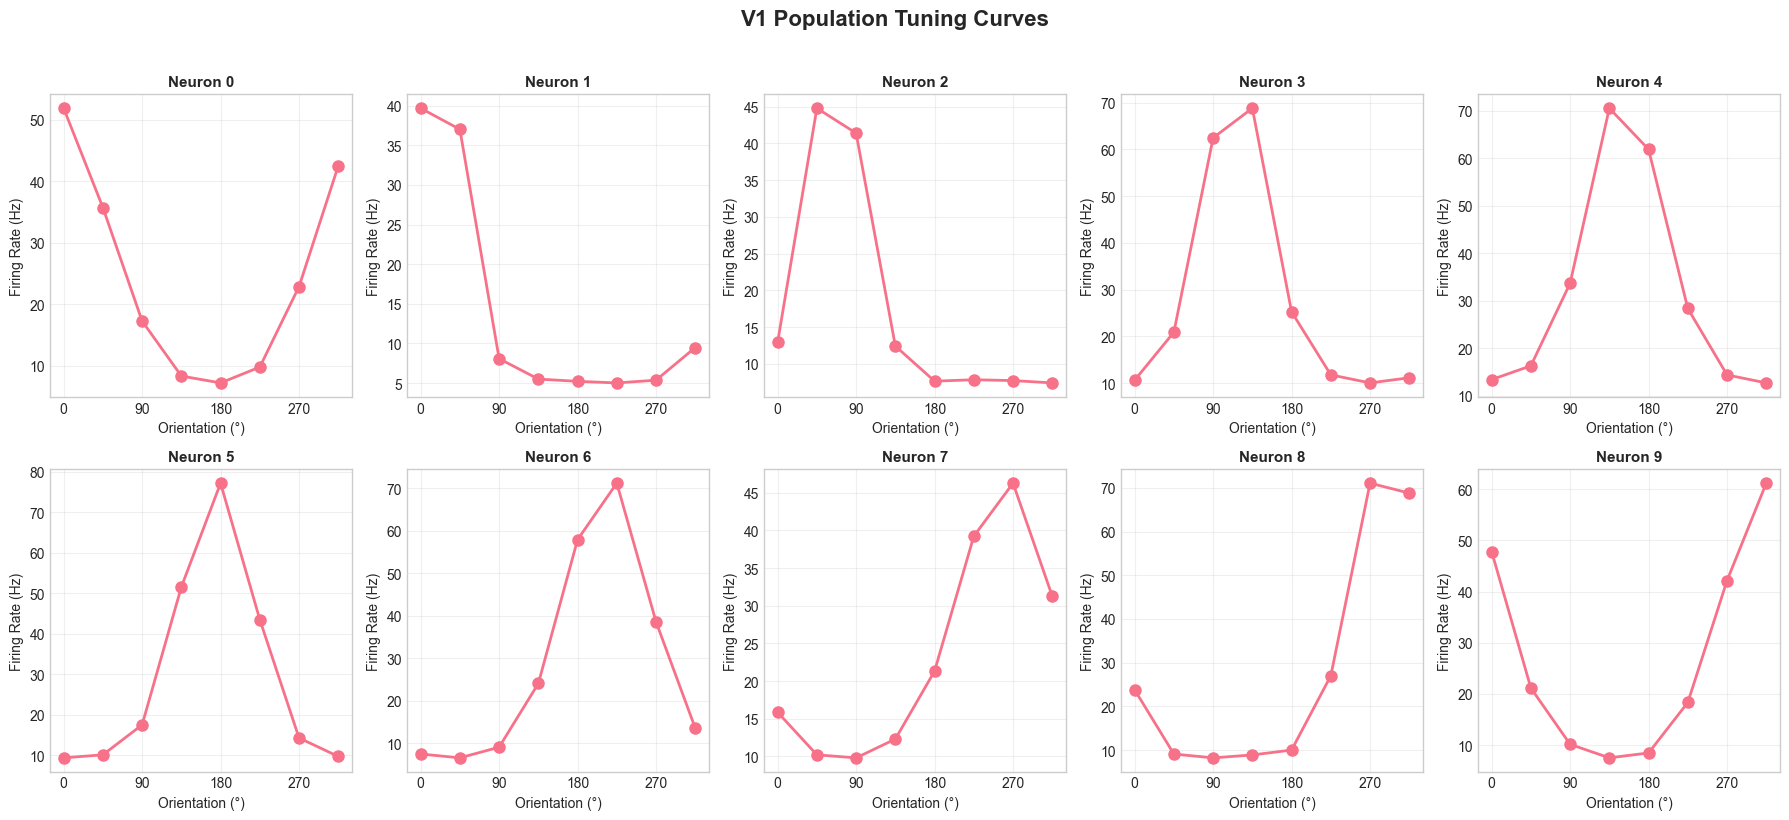
\includegraphics[keepaspectratio]{03_hoi_higher_order_interactions_files/figure-pdf/cell-11-output-2.png}}

\begin{verbatim}

✓ Population exhibits realistic orientation selectivity
  Now let's discover the information structure...
\end{verbatim}

\subsection{Discovering Synergistic
Triplets}\label{discovering-synergistic-triplets}

Now comes the exciting part: using HOI to automatically discover which
triplets of neurons exhibit synergy. We'll scan through all possible
triplets and find those with negative O-information.

\begin{Shaded}
\begin{Highlighting}[]
\CommentTok{\# Scan all triplets for synergy}
\CommentTok{\# IMPORTANT: responses has shape (n\_neurons, n\_trials) from generate\_v1\_population}
\CommentTok{\# We need to TRANSPOSE it to (n\_trials, n\_neurons) for HOI!}
\NormalTok{responses\_transposed }\OperatorTok{=}\NormalTok{ responses.T  }\CommentTok{\# Now (n\_trials, n\_neurons)}

\NormalTok{n\_neurons }\OperatorTok{=}\NormalTok{ responses\_transposed.shape[}\DecValTok{1}\NormalTok{]}
\NormalTok{all\_triplets }\OperatorTok{=} \BuiltInTok{list}\NormalTok{(combinations(}\BuiltInTok{range}\NormalTok{(n\_neurons), }\DecValTok{3}\NormalTok{))}

\BuiltInTok{print}\NormalTok{(}\SpecialStringTok{f"Data shape for HOI: }\SpecialCharTok{\{}\NormalTok{responses\_transposed}\SpecialCharTok{.}\NormalTok{shape}\SpecialCharTok{\}}\SpecialStringTok{"}\NormalTok{)}
\BuiltInTok{print}\NormalTok{(}\SpecialStringTok{f"  {-} }\SpecialCharTok{\{}\NormalTok{responses\_transposed}\SpecialCharTok{.}\NormalTok{shape[}\DecValTok{0}\NormalTok{]}\SpecialCharTok{\}}\SpecialStringTok{ samples (trials)"}\NormalTok{)}
\BuiltInTok{print}\NormalTok{(}\SpecialStringTok{f"  {-} }\SpecialCharTok{\{}\NormalTok{responses\_transposed}\SpecialCharTok{.}\NormalTok{shape[}\DecValTok{1}\NormalTok{]}\SpecialCharTok{\}}\SpecialStringTok{ features (neurons)"}\NormalTok{)}
\BuiltInTok{print}\NormalTok{(}\SpecialStringTok{f"}\CharTok{\textbackslash{}n}\SpecialStringTok{Scanning }\SpecialCharTok{\{}\BuiltInTok{len}\NormalTok{(all\_triplets)}\SpecialCharTok{\}}\SpecialStringTok{ possible triplets..."}\NormalTok{)}
\BuiltInTok{print}\NormalTok{(}\StringTok{"(This may take a minute)}\CharTok{\textbackslash{}n}\StringTok{"}\NormalTok{)}

\CommentTok{\# Create model with transposed data}
\NormalTok{model\_oinfo\_v1 }\OperatorTok{=}\NormalTok{ Oinfo(responses\_transposed)}

\CommentTok{\# Compute O{-}information for all triplets}
\NormalTok{oinfo\_values }\OperatorTok{=}\NormalTok{ model\_oinfo\_v1.fit(method}\OperatorTok{=}\StringTok{\textquotesingle{}gc\textquotesingle{}}\NormalTok{, minsize}\OperatorTok{=}\DecValTok{3}\NormalTok{, maxsize}\OperatorTok{=}\DecValTok{3}\NormalTok{)}

\CommentTok{\# Convert to list for easier handling}
\NormalTok{oinfo\_list }\OperatorTok{=}\NormalTok{ [}\BuiltInTok{float}\NormalTok{(v) }\ControlFlowTok{for}\NormalTok{ v }\KeywordTok{in}\NormalTok{ oinfo\_values]}

\CommentTok{\# Find synergistic and redundant triplets}
\NormalTok{synergy\_threshold }\OperatorTok{=} \OperatorTok{{-}}\FloatTok{0.05}  \CommentTok{\# bits}
\NormalTok{redundancy\_threshold }\OperatorTok{=} \FloatTok{0.05}  \CommentTok{\# bits}

\NormalTok{synergistic }\OperatorTok{=}\NormalTok{ [(trip, val) }\ControlFlowTok{for}\NormalTok{ trip, val }\KeywordTok{in} \BuiltInTok{zip}\NormalTok{(all\_triplets, oinfo\_list) }\ControlFlowTok{if}\NormalTok{ val }\OperatorTok{\textless{}}\NormalTok{ synergy\_threshold]}
\NormalTok{redundant }\OperatorTok{=}\NormalTok{ [(trip, val) }\ControlFlowTok{for}\NormalTok{ trip, val }\KeywordTok{in} \BuiltInTok{zip}\NormalTok{(all\_triplets, oinfo\_list) }\ControlFlowTok{if}\NormalTok{ val }\OperatorTok{\textgreater{}}\NormalTok{ redundancy\_threshold]}
\NormalTok{independent }\OperatorTok{=}\NormalTok{ [(trip, val) }\ControlFlowTok{for}\NormalTok{ trip, val }\KeywordTok{in} \BuiltInTok{zip}\NormalTok{(all\_triplets, oinfo\_list) }
               \ControlFlowTok{if} \BuiltInTok{abs}\NormalTok{(val) }\OperatorTok{\textless{}=} \BuiltInTok{max}\NormalTok{(}\BuiltInTok{abs}\NormalTok{(synergy\_threshold), redundancy\_threshold)]}

\CommentTok{\# Sort by strength}
\NormalTok{synergistic.sort(key}\OperatorTok{=}\KeywordTok{lambda}\NormalTok{ x: x[}\DecValTok{1}\NormalTok{])  }\CommentTok{\# Most negative first}
\NormalTok{redundant.sort(key}\OperatorTok{=}\KeywordTok{lambda}\NormalTok{ x: x[}\DecValTok{1}\NormalTok{], reverse}\OperatorTok{=}\VariableTok{True}\NormalTok{)  }\CommentTok{\# Most positive first}

\BuiltInTok{print}\NormalTok{(}\StringTok{"O{-}Information Analysis Complete"}\NormalTok{)}
\BuiltInTok{print}\NormalTok{(}\StringTok{"="} \OperatorTok{*} \DecValTok{60}\NormalTok{)}
\BuiltInTok{print}\NormalTok{(}\SpecialStringTok{f"}\CharTok{\textbackslash{}n}\SpecialStringTok{Total triplets: }\SpecialCharTok{\{}\BuiltInTok{len}\NormalTok{(all\_triplets)}\SpecialCharTok{\}}\SpecialStringTok{"}\NormalTok{)}
\BuiltInTok{print}\NormalTok{(}\SpecialStringTok{f"  Synergistic (O \textless{} }\SpecialCharTok{\{}\NormalTok{synergy\_threshold}\SpecialCharTok{\}}\SpecialStringTok{): }\SpecialCharTok{\{}\BuiltInTok{len}\NormalTok{(synergistic)}\SpecialCharTok{\}}\SpecialStringTok{"}\NormalTok{)}
\BuiltInTok{print}\NormalTok{(}\SpecialStringTok{f"  Independent (|O| ≤ }\SpecialCharTok{\{}\BuiltInTok{abs}\NormalTok{(synergy\_threshold)}\SpecialCharTok{\}}\SpecialStringTok{): }\SpecialCharTok{\{}\BuiltInTok{len}\NormalTok{(independent)}\SpecialCharTok{\}}\SpecialStringTok{"}\NormalTok{)}
\BuiltInTok{print}\NormalTok{(}\SpecialStringTok{f"  Redundant (O \textgreater{} }\SpecialCharTok{\{}\NormalTok{redundancy\_threshold}\SpecialCharTok{\}}\SpecialStringTok{): }\SpecialCharTok{\{}\BuiltInTok{len}\NormalTok{(redundant)}\SpecialCharTok{\}}\SpecialStringTok{"}\NormalTok{)}

\CommentTok{\# Show top synergistic triplets}
\BuiltInTok{print}\NormalTok{(}\StringTok{"}\CharTok{\textbackslash{}n}\StringTok{Top 5 Most Synergistic Triplets:"}\NormalTok{)}
\BuiltInTok{print}\NormalTok{(}\StringTok{"="} \OperatorTok{*} \DecValTok{60}\NormalTok{)}
\ControlFlowTok{for}\NormalTok{ i, (triplet, oinfo) }\KeywordTok{in} \BuiltInTok{enumerate}\NormalTok{(synergistic[:}\DecValTok{5}\NormalTok{]):}
\NormalTok{    neuron\_ids }\OperatorTok{=} \BuiltInTok{list}\NormalTok{(triplet)}
\NormalTok{    prefs }\OperatorTok{=}\NormalTok{ [neuron\_props[n][}\StringTok{\textquotesingle{}pref\_ori\textquotesingle{}}\NormalTok{] }\ControlFlowTok{for}\NormalTok{ n }\KeywordTok{in}\NormalTok{ neuron\_ids]}
    \BuiltInTok{print}\NormalTok{(}\SpecialStringTok{f"}\SpecialCharTok{\{}\NormalTok{i}\OperatorTok{+}\DecValTok{1}\SpecialCharTok{\}}\SpecialStringTok{. Neurons }\SpecialCharTok{\{}\NormalTok{neuron\_ids}\SpecialCharTok{\}}\SpecialStringTok{: O{-}info = }\SpecialCharTok{\{}\NormalTok{oinfo}\SpecialCharTok{:.4f\}}\SpecialStringTok{ bits"}\NormalTok{)}
    \BuiltInTok{print}\NormalTok{(}\SpecialStringTok{f"   Preferred orientations: }\SpecialCharTok{\{}\NormalTok{[}\SpecialStringTok{f\textquotesingle{}}\SpecialCharTok{\{}\NormalTok{p}\SpecialCharTok{:.1f\}}\SpecialStringTok{°\textquotesingle{}} \ControlFlowTok{for}\NormalTok{ p }\KeywordTok{in}\NormalTok{ prefs]}\SpecialCharTok{\}}\SpecialStringTok{"}\NormalTok{)}

\CommentTok{\# Show top redundant triplets}
\BuiltInTok{print}\NormalTok{(}\StringTok{"}\CharTok{\textbackslash{}n}\StringTok{Top 5 Most Redundant Triplets:"}\NormalTok{)}
\BuiltInTok{print}\NormalTok{(}\StringTok{"="} \OperatorTok{*} \DecValTok{60}\NormalTok{)}
\ControlFlowTok{for}\NormalTok{ i, (triplet, oinfo) }\KeywordTok{in} \BuiltInTok{enumerate}\NormalTok{(redundant[:}\DecValTok{5}\NormalTok{]):}
\NormalTok{    neuron\_ids }\OperatorTok{=} \BuiltInTok{list}\NormalTok{(triplet)}
\NormalTok{    prefs }\OperatorTok{=}\NormalTok{ [neuron\_props[n][}\StringTok{\textquotesingle{}pref\_ori\textquotesingle{}}\NormalTok{] }\ControlFlowTok{for}\NormalTok{ n }\KeywordTok{in}\NormalTok{ neuron\_ids]}
    \BuiltInTok{print}\NormalTok{(}\SpecialStringTok{f"}\SpecialCharTok{\{}\NormalTok{i}\OperatorTok{+}\DecValTok{1}\SpecialCharTok{\}}\SpecialStringTok{. Neurons }\SpecialCharTok{\{}\NormalTok{neuron\_ids}\SpecialCharTok{\}}\SpecialStringTok{: O{-}info = }\SpecialCharTok{\{}\NormalTok{oinfo}\SpecialCharTok{:.4f\}}\SpecialStringTok{ bits"}\NormalTok{)}
    \BuiltInTok{print}\NormalTok{(}\SpecialStringTok{f"   Preferred orientations: }\SpecialCharTok{\{}\NormalTok{[}\SpecialStringTok{f\textquotesingle{}}\SpecialCharTok{\{}\NormalTok{p}\SpecialCharTok{:.1f\}}\SpecialStringTok{°\textquotesingle{}} \ControlFlowTok{for}\NormalTok{ p }\KeywordTok{in}\NormalTok{ prefs]}\SpecialCharTok{\}}\SpecialStringTok{"}\NormalTok{)}

\CommentTok{\# Visualize distribution}
\NormalTok{fig, axes }\OperatorTok{=}\NormalTok{ plt.subplots(}\DecValTok{1}\NormalTok{, }\DecValTok{2}\NormalTok{, figsize}\OperatorTok{=}\NormalTok{(}\DecValTok{14}\NormalTok{, }\DecValTok{5}\NormalTok{))}

\CommentTok{\# Histogram}
\NormalTok{ax1 }\OperatorTok{=}\NormalTok{ axes[}\DecValTok{0}\NormalTok{]}
\NormalTok{ax1.hist(oinfo\_list, bins}\OperatorTok{=}\DecValTok{30}\NormalTok{, color}\OperatorTok{=}\StringTok{\textquotesingle{}\#457B9D\textquotesingle{}}\NormalTok{, alpha}\OperatorTok{=}\FloatTok{0.7}\NormalTok{, edgecolor}\OperatorTok{=}\StringTok{\textquotesingle{}black\textquotesingle{}}\NormalTok{)}
\NormalTok{ax1.axvline(x}\OperatorTok{=}\DecValTok{0}\NormalTok{, color}\OperatorTok{=}\StringTok{\textquotesingle{}black\textquotesingle{}}\NormalTok{, linestyle}\OperatorTok{=}\StringTok{\textquotesingle{}{-}\textquotesingle{}}\NormalTok{, linewidth}\OperatorTok{=}\DecValTok{2}\NormalTok{)}
\NormalTok{ax1.axvline(x}\OperatorTok{=}\NormalTok{synergy\_threshold, color}\OperatorTok{=}\StringTok{\textquotesingle{}red\textquotesingle{}}\NormalTok{, linestyle}\OperatorTok{=}\StringTok{\textquotesingle{}{-}{-}\textquotesingle{}}\NormalTok{, alpha}\OperatorTok{=}\FloatTok{0.7}\NormalTok{, label}\OperatorTok{=}\StringTok{\textquotesingle{}Synergy threshold\textquotesingle{}}\NormalTok{)}
\NormalTok{ax1.axvline(x}\OperatorTok{=}\NormalTok{redundancy\_threshold, color}\OperatorTok{=}\StringTok{\textquotesingle{}blue\textquotesingle{}}\NormalTok{, linestyle}\OperatorTok{=}\StringTok{\textquotesingle{}{-}{-}\textquotesingle{}}\NormalTok{, alpha}\OperatorTok{=}\FloatTok{0.7}\NormalTok{, label}\OperatorTok{=}\StringTok{\textquotesingle{}Redundancy threshold\textquotesingle{}}\NormalTok{)}
\NormalTok{ax1.set\_xlabel(}\StringTok{\textquotesingle{}O{-}Information (bits)\textquotesingle{}}\NormalTok{, fontsize}\OperatorTok{=}\DecValTok{12}\NormalTok{, fontweight}\OperatorTok{=}\StringTok{\textquotesingle{}bold\textquotesingle{}}\NormalTok{)}
\NormalTok{ax1.set\_ylabel(}\StringTok{\textquotesingle{}Count\textquotesingle{}}\NormalTok{, fontsize}\OperatorTok{=}\DecValTok{12}\NormalTok{, fontweight}\OperatorTok{=}\StringTok{\textquotesingle{}bold\textquotesingle{}}\NormalTok{)}
\NormalTok{ax1.set\_title(}\StringTok{\textquotesingle{}Distribution of O{-}Information Across Triplets\textquotesingle{}}\NormalTok{, fontsize}\OperatorTok{=}\DecValTok{14}\NormalTok{, fontweight}\OperatorTok{=}\StringTok{\textquotesingle{}bold\textquotesingle{}}\NormalTok{)}
\NormalTok{ax1.legend()}
\NormalTok{ax1.grid(}\VariableTok{True}\NormalTok{, alpha}\OperatorTok{=}\FloatTok{0.3}\NormalTok{)}

\CommentTok{\# Category breakdown}
\NormalTok{ax2 }\OperatorTok{=}\NormalTok{ axes[}\DecValTok{1}\NormalTok{]}
\NormalTok{categories }\OperatorTok{=}\NormalTok{ [}\StringTok{\textquotesingle{}Synergistic\textquotesingle{}}\NormalTok{, }\StringTok{\textquotesingle{}Independent\textquotesingle{}}\NormalTok{, }\StringTok{\textquotesingle{}Redundant\textquotesingle{}}\NormalTok{]}
\NormalTok{counts }\OperatorTok{=}\NormalTok{ [}\BuiltInTok{len}\NormalTok{(synergistic), }\BuiltInTok{len}\NormalTok{(independent), }\BuiltInTok{len}\NormalTok{(redundant)]}
\NormalTok{colors }\OperatorTok{=}\NormalTok{ [}\StringTok{\textquotesingle{}\#E63946\textquotesingle{}}\NormalTok{, }\StringTok{\textquotesingle{}\#A8DADC\textquotesingle{}}\NormalTok{, }\StringTok{\textquotesingle{}\#457B9D\textquotesingle{}}\NormalTok{]}
\NormalTok{ax2.bar(categories, counts, color}\OperatorTok{=}\NormalTok{colors, alpha}\OperatorTok{=}\FloatTok{0.7}\NormalTok{, edgecolor}\OperatorTok{=}\StringTok{\textquotesingle{}black\textquotesingle{}}\NormalTok{, linewidth}\OperatorTok{=}\DecValTok{2}\NormalTok{)}
\NormalTok{ax2.set\_ylabel(}\StringTok{\textquotesingle{}Number of Triplets\textquotesingle{}}\NormalTok{, fontsize}\OperatorTok{=}\DecValTok{12}\NormalTok{, fontweight}\OperatorTok{=}\StringTok{\textquotesingle{}bold\textquotesingle{}}\NormalTok{)}
\NormalTok{ax2.set\_title(}\StringTok{\textquotesingle{}Triplet Classification\textquotesingle{}}\NormalTok{, fontsize}\OperatorTok{=}\DecValTok{14}\NormalTok{, fontweight}\OperatorTok{=}\StringTok{\textquotesingle{}bold\textquotesingle{}}\NormalTok{)}
\NormalTok{ax2.grid(}\VariableTok{True}\NormalTok{, alpha}\OperatorTok{=}\FloatTok{0.3}\NormalTok{, axis}\OperatorTok{=}\StringTok{\textquotesingle{}y\textquotesingle{}}\NormalTok{)}
\ControlFlowTok{for}\NormalTok{ i, (cat, cnt) }\KeywordTok{in} \BuiltInTok{enumerate}\NormalTok{(}\BuiltInTok{zip}\NormalTok{(categories, counts)):}
\NormalTok{    ax2.text(i, cnt }\OperatorTok{+} \DecValTok{1}\NormalTok{, }\BuiltInTok{str}\NormalTok{(cnt), ha}\OperatorTok{=}\StringTok{\textquotesingle{}center\textquotesingle{}}\NormalTok{, fontweight}\OperatorTok{=}\StringTok{\textquotesingle{}bold\textquotesingle{}}\NormalTok{, fontsize}\OperatorTok{=}\DecValTok{12}\NormalTok{)}

\NormalTok{plt.tight\_layout()}
\NormalTok{plt.show()}
\end{Highlighting}
\end{Shaded}

\begin{verbatim}
Data shape for HOI: (500, 10)
  - 500 samples (trials)
  - 10 features (neurons)

Scanning 120 possible triplets...
(This may take a minute)
\end{verbatim}

\begin{verbatim}
O-Information Analysis Complete
============================================================

Total triplets: 120
  Synergistic (O < -0.05): 40
  Independent (|O| ≤ 0.05): 35
  Redundant (O > 0.05): 45

Top 5 Most Synergistic Triplets:
============================================================
1. Neurons [4, 6, 7]: O-info = -0.2586 bits
   Preferred orientations: ['151.8°', '213.4°', '260.9°']
2. Neurons [6, 7, 9]: O-info = -0.2380 bits
   Preferred orientations: ['213.4°', '260.9°', '320.0°']
3. Neurons [0, 3, 6]: O-info = -0.2216 bits
   Preferred orientations: ['-8.5°', '115.3°', '213.4°']
4. Neurons [5, 6, 8]: O-info = -0.2178 bits
   Preferred orientations: ['175.2°', '213.4°', '290.1°']
5. Neurons [0, 6, 8]: O-info = -0.2041 bits
   Preferred orientations: ['-8.5°', '213.4°', '290.1°']

Top 5 Most Redundant Triplets:
============================================================
1. Neurons [0, 4, 5]: O-info = 0.3829 bits
   Preferred orientations: ['-8.5°', '151.8°', '175.2°']
2. Neurons [0, 4, 9]: O-info = 0.3668 bits
   Preferred orientations: ['-8.5°', '151.8°', '320.0°']
3. Neurons [4, 5, 9]: O-info = 0.3489 bits
   Preferred orientations: ['151.8°', '175.2°', '320.0°']
4. Neurons [0, 5, 9]: O-info = 0.3452 bits
   Preferred orientations: ['-8.5°', '175.2°', '320.0°']
5. Neurons [3, 4, 9]: O-info = 0.3242 bits
   Preferred orientations: ['115.3°', '151.8°', '320.0°']
\end{verbatim}

\pandocbounded{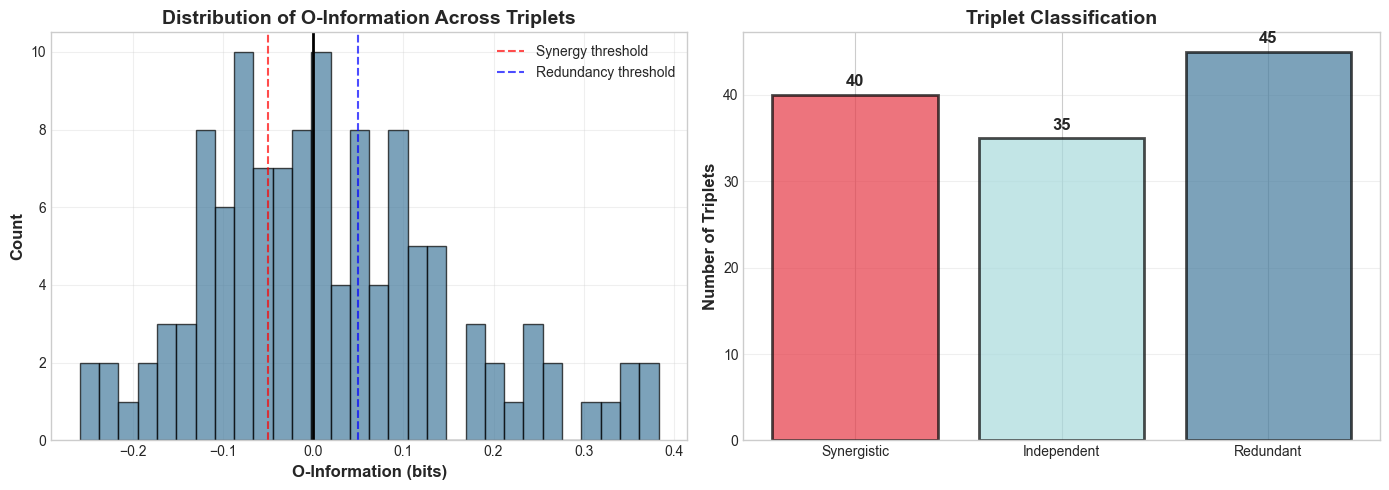
\includegraphics[keepaspectratio]{03_hoi_higher_order_interactions_files/figure-pdf/cell-12-output-3.png}}

\section{Part 6: Computational Scaling and Practical
Considerations}\label{part-6-computational-scaling-and-practical-considerations}

\subsection{The Combinatorial
Explosion}\label{the-combinatorial-explosion}

As you just saw, we computed O-information for 120 triplets (10 choose
3). But what if we had 20 neurons? Or 100? The number of possible
triplets grows \textbf{very quickly}:

\begin{itemize}
\tightlist
\item
  10 neurons: 120 triplets
\item
  20 neurons: 1,140 triplets
\item
  50 neurons: 19,600 triplets
\item
  100 neurons: 161,700 triplets
\end{itemize}

And this is just for triplets! For 4-way interactions (quadruplets), the
numbers are even larger.

\subsection{Strategies for Large
Systems}\label{strategies-for-large-systems}

When dealing with large neural populations, you need smart strategies:

\begin{enumerate}
\def\labelenumi{\arabic{enumi}.}
\tightlist
\item
  \textbf{Pre-screening}: Use pairwise MI to identify interesting
  variable pairs first
\item
  \textbf{Hierarchical}: Start with triplets, only explore larger
  multiplets if warranted
\item
  \textbf{Sampling}: Randomly sample multiplets rather than exhaustive
  search
\item
  \textbf{GPU acceleration}: Use JAX's GPU capabilities for parallel
  computation
\item
  \textbf{Time windowing}: For time series, analyze shorter windows
\end{enumerate}

Let's demonstrate some of these strategies:

\begin{Shaded}
\begin{Highlighting}[]
\CommentTok{\# Benchmark computation time vs system size}
\ImportTok{import}\NormalTok{ time}

\KeywordTok{def}\NormalTok{ benchmark\_hoi(n\_neurons\_list, n\_samples}\OperatorTok{=}\DecValTok{1000}\NormalTok{, n\_multiplets}\OperatorTok{=}\DecValTok{50}\NormalTok{):}
    \CommentTok{"""}
\CommentTok{    Measure HOI computation time for different system sizes.}
\CommentTok{    """}
\NormalTok{    results }\OperatorTok{=}\NormalTok{ []}
    
    \ControlFlowTok{for}\NormalTok{ n\_neurons }\KeywordTok{in}\NormalTok{ n\_neurons\_list:}
        \CommentTok{\# Generate random data in correct format: (n\_samples, n\_features)}
\NormalTok{        data }\OperatorTok{=}\NormalTok{ np.random.randn(n\_samples, n\_neurons)}
        
        \CommentTok{\# Sample multiplets}
\NormalTok{        all\_trips }\OperatorTok{=} \BuiltInTok{list}\NormalTok{(combinations(}\BuiltInTok{range}\NormalTok{(n\_neurons), }\DecValTok{3}\NormalTok{))}
        \ControlFlowTok{if} \BuiltInTok{len}\NormalTok{(all\_trips) }\OperatorTok{\textgreater{}}\NormalTok{ n\_multiplets:}
\NormalTok{            sampled\_trips }\OperatorTok{=}\NormalTok{ [all\_trips[i] }\ControlFlowTok{for}\NormalTok{ i }\KeywordTok{in} 
\NormalTok{                           np.random.choice(}\BuiltInTok{len}\NormalTok{(all\_trips), n\_multiplets, replace}\OperatorTok{=}\VariableTok{False}\NormalTok{)]}
        \ControlFlowTok{else}\NormalTok{:}
\NormalTok{            sampled\_trips }\OperatorTok{=}\NormalTok{ all\_trips}
        
        \CommentTok{\# Create model WITH DATA}
\NormalTok{        model }\OperatorTok{=}\NormalTok{ Oinfo(data)}
        
        \CommentTok{\# Time the computation}
\NormalTok{        start }\OperatorTok{=}\NormalTok{ time.time()}
\NormalTok{        oinfo }\OperatorTok{=}\NormalTok{ model.fit(method}\OperatorTok{=}\StringTok{\textquotesingle{}gc\textquotesingle{}}\NormalTok{, minsize}\OperatorTok{=}\DecValTok{3}\NormalTok{, maxsize}\OperatorTok{=}\DecValTok{3}\NormalTok{)}
\NormalTok{        elapsed }\OperatorTok{=}\NormalTok{ time.time() }\OperatorTok{{-}}\NormalTok{ start}
        
\NormalTok{        results.append(\{}
            \StringTok{\textquotesingle{}n\_neurons\textquotesingle{}}\NormalTok{: n\_neurons,}
            \StringTok{\textquotesingle{}n\_multiplets\textquotesingle{}}\NormalTok{: }\BuiltInTok{len}\NormalTok{(sampled\_trips),}
            \StringTok{\textquotesingle{}time\textquotesingle{}}\NormalTok{: elapsed,}
            \StringTok{\textquotesingle{}time\_per\_multiplet\textquotesingle{}}\NormalTok{: elapsed }\OperatorTok{/} \BuiltInTok{len}\NormalTok{(sampled\_trips)}
\NormalTok{        \})}
    
    \ControlFlowTok{return}\NormalTok{ results}

\CommentTok{\# Test different sizes}
\NormalTok{sizes }\OperatorTok{=}\NormalTok{ [}\DecValTok{5}\NormalTok{, }\DecValTok{10}\NormalTok{, }\DecValTok{15}\NormalTok{, }\DecValTok{20}\NormalTok{, }\DecValTok{30}\NormalTok{]}
\BuiltInTok{print}\NormalTok{(}\StringTok{"Benchmarking HOI Computation...}\CharTok{\textbackslash{}n}\StringTok{"}\NormalTok{)}
\NormalTok{benchmark\_results }\OperatorTok{=}\NormalTok{ benchmark\_hoi(sizes)}

\CommentTok{\# Display results}
\BuiltInTok{print}\NormalTok{(}\StringTok{"Computational Scaling Analysis"}\NormalTok{)}
\BuiltInTok{print}\NormalTok{(}\StringTok{"="} \OperatorTok{*} \DecValTok{70}\NormalTok{)}
\BuiltInTok{print}\NormalTok{(}\SpecialStringTok{f"}\SpecialCharTok{\{}\StringTok{\textquotesingle{}Neurons\textquotesingle{}}\SpecialCharTok{:\textless{}10\}}\SpecialStringTok{ }\SpecialCharTok{\{}\StringTok{\textquotesingle{}Multiplets\textquotesingle{}}\SpecialCharTok{:\textless{}12\}}\SpecialStringTok{ }\SpecialCharTok{\{}\StringTok{\textquotesingle{}Time (s)\textquotesingle{}}\SpecialCharTok{:\textless{}12\}}\SpecialStringTok{ }\SpecialCharTok{\{}\StringTok{\textquotesingle{}ms/multiplet\textquotesingle{}}\SpecialCharTok{:\textless{}15\}}\SpecialStringTok{"}\NormalTok{)}
\BuiltInTok{print}\NormalTok{(}\StringTok{"="} \OperatorTok{*} \DecValTok{70}\NormalTok{)}
\ControlFlowTok{for}\NormalTok{ res }\KeywordTok{in}\NormalTok{ benchmark\_results:}
    \BuiltInTok{print}\NormalTok{(}\SpecialStringTok{f"}\SpecialCharTok{\{}\NormalTok{res[}\StringTok{\textquotesingle{}n\_neurons\textquotesingle{}}\NormalTok{]}\SpecialCharTok{:\textless{}10\}}\SpecialStringTok{ }\SpecialCharTok{\{}\NormalTok{res[}\StringTok{\textquotesingle{}n\_multiplets\textquotesingle{}}\NormalTok{]}\SpecialCharTok{:\textless{}12\}}\SpecialStringTok{ "}
          \SpecialStringTok{f"}\SpecialCharTok{\{}\NormalTok{res[}\StringTok{\textquotesingle{}time\textquotesingle{}}\NormalTok{]}\SpecialCharTok{:\textless{}12.4f\}}\SpecialStringTok{ }\SpecialCharTok{\{}\NormalTok{res[}\StringTok{\textquotesingle{}time\_per\_multiplet\textquotesingle{}}\NormalTok{]}\OperatorTok{*}\DecValTok{1000}\SpecialCharTok{:\textless{}15.2f\}}\SpecialStringTok{"}\NormalTok{)}

\CommentTok{\# Visualize scaling}
\NormalTok{fig, (ax1, ax2) }\OperatorTok{=}\NormalTok{ plt.subplots(}\DecValTok{1}\NormalTok{, }\DecValTok{2}\NormalTok{, figsize}\OperatorTok{=}\NormalTok{(}\DecValTok{14}\NormalTok{, }\DecValTok{5}\NormalTok{))}

\NormalTok{neurons }\OperatorTok{=}\NormalTok{ [r[}\StringTok{\textquotesingle{}n\_neurons\textquotesingle{}}\NormalTok{] }\ControlFlowTok{for}\NormalTok{ r }\KeywordTok{in}\NormalTok{ benchmark\_results]}
\NormalTok{times }\OperatorTok{=}\NormalTok{ [r[}\StringTok{\textquotesingle{}time\textquotesingle{}}\NormalTok{] }\ControlFlowTok{for}\NormalTok{ r }\KeywordTok{in}\NormalTok{ benchmark\_results]}
\NormalTok{time\_per }\OperatorTok{=}\NormalTok{ [r[}\StringTok{\textquotesingle{}time\_per\_multiplet\textquotesingle{}}\NormalTok{]}\OperatorTok{*}\DecValTok{1000} \ControlFlowTok{for}\NormalTok{ r }\KeywordTok{in}\NormalTok{ benchmark\_results]}

\CommentTok{\# Total time}
\NormalTok{ax1.plot(neurons, times, }\StringTok{\textquotesingle{}o{-}\textquotesingle{}}\NormalTok{, linewidth}\OperatorTok{=}\DecValTok{2}\NormalTok{, markersize}\OperatorTok{=}\DecValTok{10}\NormalTok{, color}\OperatorTok{=}\StringTok{\textquotesingle{}\#E63946\textquotesingle{}}\NormalTok{)}
\NormalTok{ax1.set\_xlabel(}\StringTok{\textquotesingle{}Number of Neurons\textquotesingle{}}\NormalTok{, fontsize}\OperatorTok{=}\DecValTok{12}\NormalTok{, fontweight}\OperatorTok{=}\StringTok{\textquotesingle{}bold\textquotesingle{}}\NormalTok{)}
\NormalTok{ax1.set\_ylabel(}\StringTok{\textquotesingle{}Total Time (s)\textquotesingle{}}\NormalTok{, fontsize}\OperatorTok{=}\DecValTok{12}\NormalTok{, fontweight}\OperatorTok{=}\StringTok{\textquotesingle{}bold\textquotesingle{}}\NormalTok{)}
\NormalTok{ax1.set\_title(}\StringTok{\textquotesingle{}Total Computation Time\textquotesingle{}}\NormalTok{, fontsize}\OperatorTok{=}\DecValTok{14}\NormalTok{, fontweight}\OperatorTok{=}\StringTok{\textquotesingle{}bold\textquotesingle{}}\NormalTok{)}
\NormalTok{ax1.grid(}\VariableTok{True}\NormalTok{, alpha}\OperatorTok{=}\FloatTok{0.3}\NormalTok{)}

\CommentTok{\# Time per multiplet}
\NormalTok{ax2.plot(neurons, time\_per, }\StringTok{\textquotesingle{}o{-}\textquotesingle{}}\NormalTok{, linewidth}\OperatorTok{=}\DecValTok{2}\NormalTok{, markersize}\OperatorTok{=}\DecValTok{10}\NormalTok{, color}\OperatorTok{=}\StringTok{\textquotesingle{}\#457B9D\textquotesingle{}}\NormalTok{)}
\NormalTok{ax2.set\_xlabel(}\StringTok{\textquotesingle{}Number of Neurons\textquotesingle{}}\NormalTok{, fontsize}\OperatorTok{=}\DecValTok{12}\NormalTok{, fontweight}\OperatorTok{=}\StringTok{\textquotesingle{}bold\textquotesingle{}}\NormalTok{)}
\NormalTok{ax2.set\_ylabel(}\StringTok{\textquotesingle{}Time per Multiplet (ms)\textquotesingle{}}\NormalTok{, fontsize}\OperatorTok{=}\DecValTok{12}\NormalTok{, fontweight}\OperatorTok{=}\StringTok{\textquotesingle{}bold\textquotesingle{}}\NormalTok{)}
\NormalTok{ax2.set\_title(}\StringTok{\textquotesingle{}Per{-}Multiplet Computation Time\textquotesingle{}}\NormalTok{, fontsize}\OperatorTok{=}\DecValTok{14}\NormalTok{, fontweight}\OperatorTok{=}\StringTok{\textquotesingle{}bold\textquotesingle{}}\NormalTok{)}
\NormalTok{ax2.grid(}\VariableTok{True}\NormalTok{, alpha}\OperatorTok{=}\FloatTok{0.3}\NormalTok{)}

\NormalTok{plt.tight\_layout()}
\NormalTok{plt.show()}

\BuiltInTok{print}\NormalTok{(}\StringTok{"}\CharTok{\textbackslash{}n}\StringTok{💡 Scaling Notes:"}\NormalTok{)}
\BuiltInTok{print}\NormalTok{(}\StringTok{"  {-} Time grows with number of neurons (more entropy calculations)"}\NormalTok{)}
\BuiltInTok{print}\NormalTok{(}\StringTok{"  {-} Time per multiplet is relatively constant"}\NormalTok{)}
\BuiltInTok{print}\NormalTok{(}\StringTok{"  {-} For large systems, sample multiplets rather than computing all"}\NormalTok{)}
\end{Highlighting}
\end{Shaded}

\begin{verbatim}
Benchmarking HOI Computation...
\end{verbatim}

\begin{verbatim}
Computational Scaling Analysis
======================================================================
Neurons    Multiplets   Time (s)     ms/multiplet   
======================================================================
5          10           0.1566       15.66          
10         50           0.0748       1.50           
15         50           0.0842       1.68           
20         50           0.0961       1.92           
30         50           0.1655       3.31           
\end{verbatim}

\pandocbounded{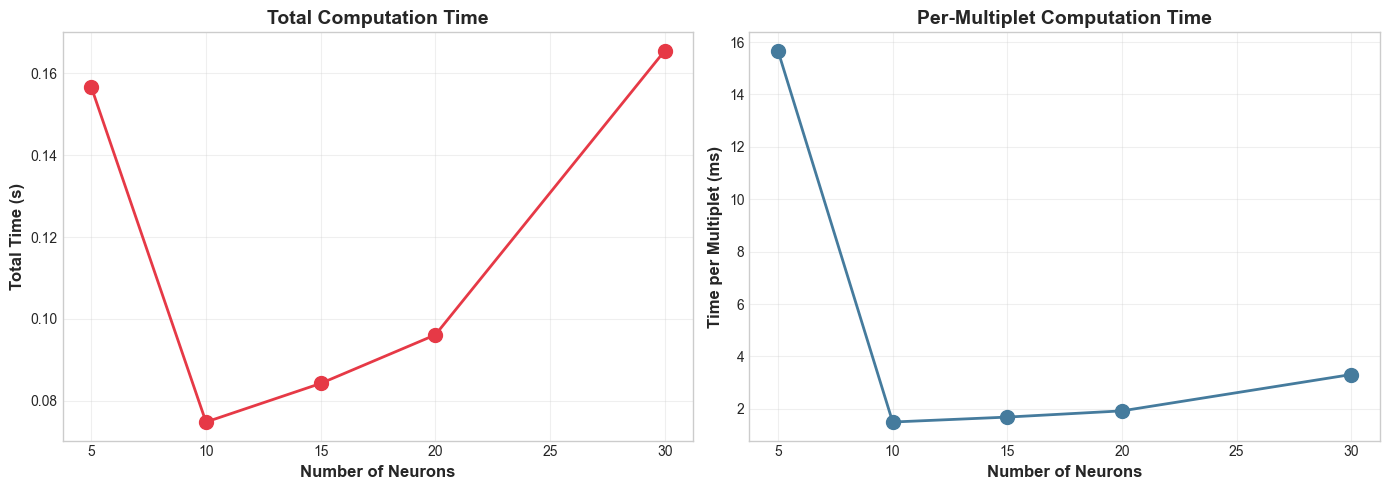
\includegraphics[keepaspectratio]{03_hoi_higher_order_interactions_files/figure-pdf/cell-13-output-3.png}}

\begin{verbatim}

💡 Scaling Notes:
  - Time grows with number of neurons (more entropy calculations)
  - Time per multiplet is relatively constant
  - For large systems, sample multiplets rather than computing all
\end{verbatim}

\section{Summary and Key Takeaways}\label{summary-and-key-takeaways}

\subsection{What We've Accomplished}\label{what-weve-accomplished}

Congratulations! You've gone from manual calculations in Notebooks 1-2
to using a professional package for higher-order interaction analysis.
You now know how to:

\begin{enumerate}
\def\labelenumi{\arabic{enumi}.}
\tightlist
\item
  \textbf{Install and configure HOI} with the right estimators
\item
  \textbf{Compute O-information} to detect synergy vs redundancy
\item
  \textbf{Apply PID} to decompose information into four atoms
\item
  \textbf{Use multiple estimators} and understand their trade-offs
\item
  \textbf{Analyze realistic neural data} to discover information
  structure
\item
  \textbf{Understand computational scaling} and plan analyses
  appropriately
\end{enumerate}

\subsection{When to Use Each HOI
Measure}\label{when-to-use-each-hoi-measure}

\textbf{O-Information (\texttt{Oinfo})}: - \textbf{Use for}: Quick
screening to identify synergistic or redundant multiplets -
\textbf{Advantages}: Fast, single number, clear interpretation -
\textbf{Limitations}: Doesn't decompose into
unique/redundant/synergistic components

\textbf{PID (RedundancyMMI + SynergyMMI)}: - \textbf{Use for}: Detailed
understanding of information structure (2 sources only) -
\textbf{Advantages}: Complete decomposition into interpretable atoms -
\textbf{Limitations}: Only well-defined for 2 sources, computationally
expensive

\textbf{Total Correlation (\texttt{TC})}: - \textbf{Use for}: Measuring
overall system integration - \textbf{Advantages}: Always non-negative,
intuitive - \textbf{Limitations}: Doesn't distinguish synergy from
redundancy

\subsection{Critical Reminders}\label{critical-reminders}

\textbf{Data Format}: HOI expects (n\_features, n\_samples) - opposite
of scikit-learn!

\textbf{Estimator Choice}: Use `gc' (Gaussian Copula) as default unless
you have specific reasons otherwise.

\textbf{Statistical Significance}: HOI doesn't include built-in
significance testing. For that, use Frites (next notebook) or implement
permutation tests.

\textbf{Interpretation}: Always report both sign AND magnitude of
O-information.

\textbf{Computational Planning}: For large systems (50+ variables), use
sampling or hierarchical strategies.

\subsection{The Bigger Picture}\label{the-bigger-picture}

HOI has revealed something profound about your V1 population: some
neuron triplets carry information synergistically (their combination
predicts better than the sum of individuals), while others are redundant
(they duplicate information for robustness).

This isn't just a mathematical curiosity - it reflects the
\textbf{functional organization} of neural circuits. Synergistic
triplets might correspond to neurons within the same orientation column
working together. Redundant triplets might provide robustness against
noise or damage.

\subsection{Bridge to Notebook 4}\label{bridge-to-notebook-4}

HOI is excellent for analyzing static snapshots of neural activity. But
real neural data is \textbf{dynamic} - it evolves over time during
tasks. In Notebook 4, we'll use \textbf{Frites} to: - Compute
\textbf{time-resolved} mutual information - Track how information flows
during cognitive tasks - Perform \textbf{statistical testing} with
permutations - Analyze \textbf{dynamic functional connectivity} - Handle
\textbf{multi-subject} designs properly

Frites complements HOI by adding temporal dynamics and rigorous
statistics. Together, they provide a complete toolkit for
information-theoretic analysis of neural data.

See you in Notebook 4! 🚀

\section{Practice Exercises}\label{practice-exercises-1}

Before moving to Notebook 4, try these exercises to solidify your
understanding:

\begin{Shaded}
\begin{Highlighting}[]
\BuiltInTok{print}\NormalTok{(}\StringTok{"PRACTICE EXERCISES"}\NormalTok{)}
\BuiltInTok{print}\NormalTok{(}\StringTok{"="} \OperatorTok{*} \DecValTok{70}\NormalTok{)}

\BuiltInTok{print}\NormalTok{(}\StringTok{"}\CharTok{\textbackslash{}n}\StringTok{1. Create an OR gate (Y = X₁ OR X₂) and compute its O{-}information."}\NormalTok{)}
\BuiltInTok{print}\NormalTok{(}\StringTok{"   Will it be synergistic, redundant, or independent?"}\NormalTok{)}
\BuiltInTok{print}\NormalTok{(}\StringTok{"   Hint: Think about what happens when both inputs are 1"}\NormalTok{)}

\BuiltInTok{print}\NormalTok{(}\StringTok{"}\CharTok{\textbackslash{}n}\StringTok{2. Modify the V1 simulation to have 15 neurons instead of 10."}\NormalTok{)}
\BuiltInTok{print}\NormalTok{(}\StringTok{"   How does the distribution of O{-}information values change?"}\NormalTok{)}
\BuiltInTok{print}\NormalTok{(}\StringTok{"   Are there more or fewer synergistic triplets?"}\NormalTok{)}

\BuiltInTok{print}\NormalTok{(}\StringTok{"}\CharTok{\textbackslash{}n}\StringTok{3. Compare PID decomposition for AND gate vs OR gate."}\NormalTok{)}
\BuiltInTok{print}\NormalTok{(}\StringTok{"   Which has more redundancy? Which has more synergy?"}\NormalTok{)}
\BuiltInTok{print}\NormalTok{(}\StringTok{"   Can you explain why based on the logic?"}\NormalTok{)}

\BuiltInTok{print}\NormalTok{(}\StringTok{"}\CharTok{\textbackslash{}n}\StringTok{4. Test different estimators (\textquotesingle{}gc\textquotesingle{}, \textquotesingle{}gauss\textquotesingle{}, \textquotesingle{}binning\textquotesingle{}) on Gaussian data."}\NormalTok{)}
\BuiltInTok{print}\NormalTok{(}\StringTok{"   When is \textquotesingle{}gauss\textquotesingle{} estimator most accurate?"}\NormalTok{)}
\BuiltInTok{print}\NormalTok{(}\StringTok{"   When does it fail?"}\NormalTok{)}

\BuiltInTok{print}\NormalTok{(}\StringTok{"}\CharTok{\textbackslash{}n}\StringTok{5. Add noise to the XOR system: flip Y with 30\% probability."}\NormalTok{)}
\BuiltInTok{print}\NormalTok{(}\StringTok{"   How does this affect:"}\NormalTok{)}
\BuiltInTok{print}\NormalTok{(}\StringTok{"   {-} O{-}information magnitude?"}\NormalTok{)}
\BuiltInTok{print}\NormalTok{(}\StringTok{"   {-} PID decomposition?"}\NormalTok{)}
\BuiltInTok{print}\NormalTok{(}\StringTok{"   {-} Does synergy decrease linearly with noise?"}\NormalTok{)}

\BuiltInTok{print}\NormalTok{(}\StringTok{"}\CharTok{\textbackslash{}n}\StringTok{"} \OperatorTok{+} \StringTok{"="} \OperatorTok{*} \DecValTok{70}\NormalTok{)}
\BuiltInTok{print}\NormalTok{(}\StringTok{"Try these exercises in a new cell below!"}\NormalTok{)}
\BuiltInTok{print}\NormalTok{(}\StringTok{"Solutions are in the notebook repository."}\NormalTok{)}
\BuiltInTok{print}\NormalTok{(}\StringTok{"="} \OperatorTok{*} \DecValTok{70}\NormalTok{)}
\end{Highlighting}
\end{Shaded}

\begin{verbatim}
PRACTICE EXERCISES
======================================================================

1. Create an OR gate (Y = X₁ OR X₂) and compute its O-information.
   Will it be synergistic, redundant, or independent?
   Hint: Think about what happens when both inputs are 1

2. Modify the V1 simulation to have 15 neurons instead of 10.
   How does the distribution of O-information values change?
   Are there more or fewer synergistic triplets?

3. Compare PID decomposition for AND gate vs OR gate.
   Which has more redundancy? Which has more synergy?
   Can you explain why based on the logic?

4. Test different estimators ('gc', 'gauss', 'binning') on Gaussian data.
   When is 'gauss' estimator most accurate?
   When does it fail?

5. Add noise to the XOR system: flip Y with 30% probability.
   How does this affect:
   - O-information magnitude?
   - PID decomposition?
   - Does synergy decrease linearly with noise?

======================================================================
Try these exercises in a new cell below!
Solutions are in the notebook repository.
======================================================================
\end{verbatim}

\section{Further Resources}\label{further-resources}

\subsection{HOI Documentation}\label{hoi-documentation}

\begin{itemize}
\tightlist
\item
  \textbf{Main documentation}: https://brainets.github.io/hoi/
\item
  \textbf{GitHub repository}: https://github.com/brainets/hoi
\item
  \textbf{Tutorial examples}: Check the examples gallery
\end{itemize}

\subsection{Key Papers on PID}\label{key-papers-on-pid}

\begin{enumerate}
\def\labelenumi{\arabic{enumi}.}
\tightlist
\item
  \textbf{Williams \& Beer (2010)} - ``Nonnegative Decomposition of
  Multivariate Information''

  \begin{itemize}
  \tightlist
  \item
    Original PID framework
  \item
    Defines the four atoms
  \end{itemize}
\item
  \textbf{Bertschinger et al.~(2014)} - ``Quantifying Unique
  Information''

  \begin{itemize}
  \tightlist
  \item
    BROJA measure
  \item
    Game-theoretic formulation
  \end{itemize}
\item
  \textbf{Timme et al.~(2014)} - ``Synergy, redundancy, and multivariate
  information measures''

  \begin{itemize}
  \tightlist
  \item
    Comprehensive review
  \item
    Comparison of different PID measures
  \end{itemize}
\end{enumerate}

\subsection{Related Packages}\label{related-packages}

\begin{itemize}
\tightlist
\item
  \textbf{dit}: Discrete information theory (Python)
\item
  \textbf{IDTxl}: Information dynamics (transfer entropy)
\item
  \textbf{JIDT}: Java Information Dynamics Toolkit
\item
  \textbf{Frites}: Next notebook!
\end{itemize}

\subsection{Advanced Topics}\label{advanced-topics-1}

\begin{itemize}
\tightlist
\item
  \textbf{Multiplet expansion}: Beyond triplets
\item
  \textbf{Directed information}: Causal structures
\item
  \textbf{Information geometry}: Geometric interpretation
\item
  \textbf{Integrated Information Theory (IIT)}: Consciousness and Φ
\end{itemize}

Happy exploring! 🎉

\chapter{Notebook 4: Neural Time Series Analysis with
Frites}\label{notebook-4-neural-time-series-analysis-with-frites}

\section{From Static Snapshots to Dynamic Information
Flow}\label{from-static-snapshots-to-dynamic-information-flow}

Welcome to Notebook 4! In the previous notebooks, we built a foundation
in information theory (Notebook 1), discovered the XOR problem (Notebook
2), and learned to use HOI for detecting synergy and redundancy
(Notebook 3). But there's been one crucial limitation: everything we've
done has been \textbf{static}.

Neural activity isn't static - it's a dynamic, time-varying process.
When you present a visual stimulus, neural responses evolve over time: -
Early visual areas respond within 50-100ms - Information propagates
through the cortical hierarchy - Connectivity patterns change with
cognitive states - Learning modulates information flow

\textbf{We need tools that can track information over time.}

\subsection{Enter Frites}\label{enter-frites}

\textbf{Frites} (Framework for Information Theoretical analysis of
Electrophysiological data and Statistics) is designed specifically for
M/EEG and intracranial neural data. It provides:

✨ \textbf{Time-resolved mutual information} ✨ \textbf{Statistical
testing with permutations} ✨ \textbf{Cluster-based correction for
multiple comparisons} ✨ \textbf{Dynamic functional connectivity} ✨
\textbf{Multi-subject group analysis} ✨ \textbf{Integration with
MNE-Python}

\subsection{Why Frites Matters}\label{why-frites-matters}

Frites solves two critical problems:

\begin{enumerate}
\def\labelenumi{\arabic{enumi}.}
\tightlist
\item
  \textbf{Temporal dynamics}: Compute MI at each time point to see when
  information emerges
\item
  \textbf{Statistical rigor}: Not just ``is MI high?'' but ``is it
  significantly different from chance?''
\end{enumerate}

Without proper statistics, you can't distinguish real effects from
noise. Frites handles this automatically.

\subsection{Learning Objectives}\label{learning-objectives-2}

By the end of this notebook, you'll: 1. Understand Frites' data
structure (\texttt{DatasetEphy}) 2. Compute time-resolved mutual
information 3. Apply permutation testing for significance 4. Use
cluster-based correction for multiple comparisons 5. Analyze dynamic
functional connectivity 6. Understand fixed-effect vs random-effect
analysis 7. Interpret GCMI (Gaussian Copula MI) 8. Know when to use
Frites vs HOI

Let's begin! 🧠⚡

\section{Part 1: Installation and Understanding Frites Data
Structure}\label{part-1-installation-and-understanding-frites-data-structure}

\subsection{Installation}\label{installation}

Frites integrates with MNE-Python, the standard package for M/EEG
analysis. We'll install both:

\begin{Shaded}
\begin{Highlighting}[]
\CommentTok{\# Install Frites and dependencies}
\OperatorTok{!}\NormalTok{pip install }\OperatorTok{{-}}\NormalTok{q frites mne numpy scipy matplotlib seaborn pandas xarray}

\BuiltInTok{print}\NormalTok{(}\StringTok{"Installation complete! ✓"}\NormalTok{)}
\BuiltInTok{print}\NormalTok{(}\StringTok{"Importing libraries..."}\NormalTok{)}
\end{Highlighting}
\end{Shaded}

\begin{verbatim}
Installation complete! ✓
Importing libraries...
\end{verbatim}

\begin{Shaded}
\begin{Highlighting}[]
\CommentTok{\# Import all necessary libraries}
\ImportTok{import}\NormalTok{ numpy }\ImportTok{as}\NormalTok{ np}
\ImportTok{import}\NormalTok{ matplotlib.pyplot }\ImportTok{as}\NormalTok{ plt}
\ImportTok{import}\NormalTok{ seaborn }\ImportTok{as}\NormalTok{ sns}
\ImportTok{import}\NormalTok{ pandas }\ImportTok{as}\NormalTok{ pd}
\ImportTok{import}\NormalTok{ xarray }\ImportTok{as}\NormalTok{ xr}
\ImportTok{from}\NormalTok{ scipy }\ImportTok{import}\NormalTok{ stats}
\ImportTok{import}\NormalTok{ warnings}
\NormalTok{warnings.filterwarnings(}\StringTok{\textquotesingle{}ignore\textquotesingle{}}\NormalTok{)}

\CommentTok{\# Check NumPy version for Frites compatibility}
\BuiltInTok{print}\NormalTok{(}\SpecialStringTok{f"NumPy version: }\SpecialCharTok{\{}\NormalTok{np}\SpecialCharTok{.}\NormalTok{\_\_version\_\_}\SpecialCharTok{\}}\SpecialStringTok{"}\NormalTok{)}
\NormalTok{numpy\_major\_version }\OperatorTok{=} \BuiltInTok{int}\NormalTok{(np.\_\_version\_\_.split(}\StringTok{\textquotesingle{}.\textquotesingle{}}\NormalTok{)[}\DecValTok{0}\NormalTok{])}

\ControlFlowTok{if}\NormalTok{ numpy\_major\_version }\OperatorTok{\textgreater{}=} \DecValTok{2}\NormalTok{:}
    \BuiltInTok{print}\NormalTok{(}\StringTok{"}\CharTok{\textbackslash{}n}\StringTok{⚠️  WARNING: NumPy 2.0+ detected"}\NormalTok{)}
    \BuiltInTok{print}\NormalTok{(}\StringTok{"   Frites requires NumPy 1.x for compatibility"}\NormalTok{)}
    \BuiltInTok{print}\NormalTok{(}\StringTok{"}\CharTok{\textbackslash{}n}\StringTok{   FIX: Run in terminal:"}\NormalTok{)}
    \BuiltInTok{print}\NormalTok{(}\StringTok{"   pip install \textquotesingle{}numpy\textless{}2.0\textquotesingle{} {-}{-}force{-}reinstall"}\NormalTok{)}
    \BuiltInTok{print}\NormalTok{(}\StringTok{"   Then restart kernel and rerun this notebook}\CharTok{\textbackslash{}n}\StringTok{"}\NormalTok{)}
    \ControlFlowTok{raise} \PreprocessorTok{ImportError}\NormalTok{(}\StringTok{"NumPy 2.0+ incompatible with Frites. Please downgrade to NumPy 1.x"}\NormalTok{)}

\CommentTok{\# Import Frites components}
\ImportTok{import}\NormalTok{ frites}
\ImportTok{from}\NormalTok{ frites.dataset }\ImportTok{import}\NormalTok{ DatasetEphy}
\ImportTok{from}\NormalTok{ frites.workflow }\ImportTok{import}\NormalTok{ WfMi, WfStats}
\ImportTok{from}\NormalTok{ frites.conn }\ImportTok{import}\NormalTok{ conn\_dfc, conn\_covgc}
\ImportTok{from}\NormalTok{ frites }\ImportTok{import}\NormalTok{ set\_mpl\_style}

\CommentTok{\# Set Frites plotting style}
\NormalTok{set\_mpl\_style()}

\CommentTok{\# Random seed}
\NormalTok{np.random.seed(}\DecValTok{42}\NormalTok{)}

\BuiltInTok{print}\NormalTok{(}\SpecialStringTok{f"✓ NumPy }\SpecialCharTok{\{}\NormalTok{np}\SpecialCharTok{.}\NormalTok{\_\_version\_\_}\SpecialCharTok{\}}\SpecialStringTok{ (compatible)"}\NormalTok{)}
\BuiltInTok{print}\NormalTok{(}\SpecialStringTok{f"✓ Frites version: }\SpecialCharTok{\{}\NormalTok{frites}\SpecialCharTok{.}\NormalTok{\_\_version\_\_}\SpecialCharTok{\}}\SpecialStringTok{"}\NormalTok{)}
\BuiltInTok{print}\NormalTok{(}\StringTok{"All libraries loaded successfully!"}\NormalTok{)}
\BuiltInTok{print}\NormalTok{(}\StringTok{"}\CharTok{\textbackslash{}n}\StringTok{🎉 Ready to analyze neural time series!"}\NormalTok{)}
\end{Highlighting}
\end{Shaded}

\begin{verbatim}
NumPy version: 1.26.4
✓ NumPy 1.26.4 (compatible)
✓ Frites version: 0.4.4
All libraries loaded successfully!

🎉 Ready to analyze neural time series!
\end{verbatim}

\subsection{Understanding Frites Data Structure:
DatasetEphy}\label{understanding-frites-data-structure-datasetephy}

Frites uses a specialized data container called \texttt{DatasetEphy}
(``Phy'' = electrophysiology). This is different from both HOI and
standard NumPy arrays, so understanding it is crucial.

\subsubsection{The DatasetEphy
Structure}\label{the-datasetephy-structure}

\begin{Shaded}
\begin{Highlighting}[]
\NormalTok{DatasetEphy(}
\NormalTok{    x,        }\CommentTok{\# Neural data: list of arrays, one per subject}
\NormalTok{    y,        }\CommentTok{\# Task variable: list of arrays, one per subject  }
\NormalTok{    roi,      }\CommentTok{\# Brain regions: list of lists, one per subject}
\NormalTok{    times     }\CommentTok{\# Time vector: shared across subjects}
\NormalTok{)}
\end{Highlighting}
\end{Shaded}

\subsubsection{Critical Format Details}\label{critical-format-details}

\textbf{Neural data (\texttt{x})}: List of arrays, each with shape
\texttt{(n\_epochs,\ n\_channels,\ n\_times)} - \texttt{n\_epochs}:
Number of trials for this subject - \texttt{n\_channels}: Number of
sensors/electrodes/brain regions - \texttt{n\_times}: Number of time
points per trial

\textbf{Task variable (\texttt{y})}: List of arrays, each with shape
\texttt{(n\_epochs,)} - Can be continuous (reaction time, stimulus
intensity) → use
\texttt{mi\_type=\textquotesingle{}cd\textquotesingle{}} - Can be
discrete (condition labels) → use
\texttt{mi\_type=\textquotesingle{}cd\textquotesingle{}}\\
- Can be another continuous neural signal → use
\texttt{mi\_type=\textquotesingle{}cc\textquotesingle{}}

\textbf{ROI names (\texttt{roi})}: List of lists of strings - Each
subject has their own list of channel names - Allows for different
electrode placements across subjects - Frites automatically finds common
ROIs

\textbf{Time vector (\texttt{times})}: Single array for all subjects -
Assumes time points are aligned - Usually in seconds

Let's create a simple example to see this in practice:

\begin{Shaded}
\begin{Highlighting}[]
\CommentTok{\# Create a minimal example with 2 subjects}
\NormalTok{n\_subjects }\OperatorTok{=} \DecValTok{2}
\NormalTok{n\_channels }\OperatorTok{=} \DecValTok{5}
\NormalTok{n\_times }\OperatorTok{=} \DecValTok{100}
\NormalTok{time }\OperatorTok{=}\NormalTok{ np.linspace(}\OperatorTok{{-}}\FloatTok{0.2}\NormalTok{, }\FloatTok{0.8}\NormalTok{, n\_times)  }\CommentTok{\# {-}200ms to 800ms}

\CommentTok{\# Initialize lists}
\NormalTok{data\_list }\OperatorTok{=}\NormalTok{ []}
\NormalTok{y\_list }\OperatorTok{=}\NormalTok{ []}
\NormalTok{roi\_list }\OperatorTok{=}\NormalTok{ []}

\ControlFlowTok{for}\NormalTok{ subj }\KeywordTok{in} \BuiltInTok{range}\NormalTok{(n\_subjects):}
    \CommentTok{\# Each subject has different number of trials}
\NormalTok{    n\_epochs }\OperatorTok{=} \DecValTok{50} \OperatorTok{+}\NormalTok{ subj }\OperatorTok{*} \DecValTok{20}  \CommentTok{\# Subject 0: 50 trials, Subject 1: 70 trials}
    
    \CommentTok{\# Neural data: (n\_epochs, n\_channels, n\_times)}
\NormalTok{    subj\_data }\OperatorTok{=}\NormalTok{ np.random.randn(n\_epochs, n\_channels, n\_times)}
\NormalTok{    data\_list.append(subj\_data)}
    
    \CommentTok{\# Task variable: continuous (e.g., stimulus intensity)}
\NormalTok{    task\_var }\OperatorTok{=}\NormalTok{ np.random.randn(n\_epochs)}
\NormalTok{    y\_list.append(task\_var)}
    
    \CommentTok{\# ROI names}
\NormalTok{    roi\_names }\OperatorTok{=}\NormalTok{ [}\SpecialStringTok{f\textquotesingle{}V1\_}\SpecialCharTok{\{}\NormalTok{i}\SpecialCharTok{\}}\SpecialStringTok{\textquotesingle{}} \ControlFlowTok{for}\NormalTok{ i }\KeywordTok{in} \BuiltInTok{range}\NormalTok{(n\_channels)]}
\NormalTok{    roi\_list.append(roi\_names)}

\CommentTok{\# Create DatasetEphy}
\NormalTok{ds }\OperatorTok{=}\NormalTok{ DatasetEphy(}
\NormalTok{    x}\OperatorTok{=}\NormalTok{data\_list,}
\NormalTok{    y}\OperatorTok{=}\NormalTok{y\_list,}
\NormalTok{    roi}\OperatorTok{=}\NormalTok{roi\_list,}
\NormalTok{    times}\OperatorTok{=}\NormalTok{time}
\NormalTok{)}

\BuiltInTok{print}\NormalTok{(}\StringTok{"DatasetEphy Created"}\NormalTok{)}
\BuiltInTok{print}\NormalTok{(}\StringTok{"="} \OperatorTok{*} \DecValTok{60}\NormalTok{)}
\BuiltInTok{print}\NormalTok{(ds)}
\BuiltInTok{print}\NormalTok{(}\StringTok{"}\CharTok{\textbackslash{}n}\StringTok{Key Properties:"}\NormalTok{)}
\BuiltInTok{print}\NormalTok{(}\SpecialStringTok{f"  Number of subjects: }\SpecialCharTok{\{}\BuiltInTok{len}\NormalTok{(data\_list)}\SpecialCharTok{\}}\SpecialStringTok{"}\NormalTok{)}
\BuiltInTok{print}\NormalTok{(}\SpecialStringTok{f"  Time points: }\SpecialCharTok{\{}\NormalTok{n\_times}\SpecialCharTok{\}}\SpecialStringTok{"}\NormalTok{)}
\BuiltInTok{print}\NormalTok{(}\SpecialStringTok{f"  Time range: }\SpecialCharTok{\{}\NormalTok{time[}\DecValTok{0}\NormalTok{]}\SpecialCharTok{:.2f\}}\SpecialStringTok{s to }\SpecialCharTok{\{}\NormalTok{time[}\OperatorTok{{-}}\DecValTok{1}\NormalTok{]}\SpecialCharTok{:.2f\}}\SpecialStringTok{s"}\NormalTok{)}
\BuiltInTok{print}\NormalTok{(}\SpecialStringTok{f"  Channels per subject: }\SpecialCharTok{\{}\NormalTok{n\_channels}\SpecialCharTok{\}}\SpecialStringTok{"}\NormalTok{)}
\BuiltInTok{print}\NormalTok{(}\SpecialStringTok{f"  Trials per subject: }\SpecialCharTok{\{}\NormalTok{[}\BuiltInTok{len}\NormalTok{(y) }\ControlFlowTok{for}\NormalTok{ y }\KeywordTok{in}\NormalTok{ y\_list]}\SpecialCharTok{\}}\SpecialStringTok{"}\NormalTok{)}
\BuiltInTok{print}\NormalTok{(}\StringTok{"}\CharTok{\textbackslash{}n}\StringTok{✓ Frites handles variable trial counts automatically!"}\NormalTok{)}
\BuiltInTok{print}\NormalTok{(}\StringTok{"  This is crucial for real experiments with dropouts"}\NormalTok{)}
\end{Highlighting}
\end{Shaded}

\begin{verbatim}
DatasetEphy Created
============================================================
<xarray.DataArray 'subject_0' (trials: 50, roi: 5, times: 100)> Size: 200kB
array([[[ 0.49671415, -0.1382643 ,  0.64768854, ...,  0.26105527,
          0.00511346, -0.23458713],
        [-1.41537074, -0.42064532, -0.34271452, ...,  0.15372511,
          0.05820872, -1.1429703 ],
        [ 0.35778736,  0.56078453,  1.08305124, ...,  0.30729952,
          0.81286212,  0.62962884],
        [-0.82899501, -0.56018104,  0.74729361, ...,  1.35387237,
         -0.11453985,  1.23781631],
        [-1.59442766, -0.59937502,  0.0052437 , ..., -0.19033868,
         -0.87561825, -1.38279973]],

       [[ 0.92617755,  1.90941664, -1.39856757, ..., -0.97876372,
         -0.44429326,  0.37730049],
        [ 0.75698862, -0.92216532,  0.86960592, ..., -1.25111358,
          0.92402702, -0.18490214],
        [-0.52272302,  1.04900923, -0.70434369, ...,  0.6815007 ,
          0.02831838,  0.02975614],
        [ 0.93828381, -0.51604473,  0.09612078, ...,  0.14671369,
          1.20650897, -0.81693567],
        [ 0.36867331, -0.39333881,  0.02874482, ...,  0.64084286,
...
          0.00878155, -1.75822163],
        [-0.23816954, -1.38637907, -1.20679589, ..., -0.83313778,
         -1.57775323, -0.78174047],
        [-1.02777392, -0.64668685, -1.32588408, ..., -0.28496951,
          0.44194438, -0.44582948],
        [-0.82703757,  0.00396218,  0.51903274, ...,  0.53212857,
         -0.68822826,  0.08059582],
        [-0.85378638,  1.50411284,  1.62287598, ...,  1.20777649,
         -1.05663821,  0.74546145]],

       [[ 0.05682406,  0.1665865 ,  0.6256229 , ...,  2.05239549,
          0.6783772 , -1.23442217],
        [-0.34540695,  0.59596331,  0.4832905 , ..., -0.46932818,
          1.21605173, -0.74699038],
        [ 0.60043308, -1.30478575,  1.03113043, ...,  0.61152167,
          0.17732836,  1.23054501],
        [ 0.24100314, -0.83059052, -0.46728062, ...,  0.93861077,
         -0.89306856, -0.49636313],
        [ 0.53563759, -2.06943926,  1.41658382, ...,  0.96777886,
          0.62369321,  0.01558457]]])
Coordinates:
  * trials   (trials) int64 400B 0 1 2 3 4 5 6 7 8 ... 42 43 44 45 46 47 48 49
    y        (trials) float64 400B 0.1709 0.01226 -0.4312 ... 0.4865 -0.1371
  * roi      (roi) <U4 80B 'V1_0' 'V1_1' 'V1_2' 'V1_3' 'V1_4'
    agg_ch   (roi) int64 40B 0 0 0 0 0
  * times    (times) float64 800B -0.2 -0.1899 -0.1798 ... 0.7798 0.7899 0.8
    subject  (trials) int64 400B 0 0 0 0 0 0 0 0 0 0 0 ... 0 0 0 0 0 0 0 0 0 0 0
Attributes:
    __version__:   0.4.4
    modality:      electrophysiology
    dtype:         SubjectEphy
    y_dtype:       float
    z_dtype:       none
    mi_type:       cc
    mi_repr:       I(x; y (continuous))
    sfreq:         98.9999999999999
    agg_ch:        1
    multivariate:  0
<xarray.DataArray 'subject_1' (trials: 70, roi: 5, times: 100)> Size: 280kB
array([[[ 0.3039018 ,  0.31685234, -0.03988675, ..., -1.13381919,
          0.22701574, -0.59042695],
        [ 0.7008291 , -0.79788682,  0.771803  , ...,  0.42248462,
         -0.90737889, -0.06223106],
        [ 1.05718454,  0.30397018, -0.72213487, ...,  0.03004136,
         -1.29643838, -0.96911934],
        [ 0.14944115, -0.4944546 , -1.04459979, ...,  2.49124833,
         -1.56374109,  0.16296167],
        [-1.17435296,  0.87984592, -1.58147543, ...,  0.04546653,
         -0.67984793,  0.51281956]],

       [[ 0.19499029, -0.85910398, -0.65880283, ...,  3.2153742 ,
          0.33205912,  0.23555221],
        [-2.15536267,  0.42794744,  0.16866776, ..., -0.17873812,
          0.86281756, -0.57175425],
        [ 0.27032125, -0.13167378, -0.61469682, ...,  0.44978262,
          0.65492445,  0.44617094],
        [-1.50698718, -1.19816095, -0.51021817, ..., -1.48993615,
         -0.09261883,  1.03011785],
        [-1.11892428,  0.01652641, -1.85460931, ...,  0.73286498,
...
         -0.7792243 ,  1.23822642],
        [-0.24402657, -0.18208393,  1.28198046, ...,  1.87401644,
         -0.66065685,  0.18771821],
        [ 0.1590628 , -1.10605157, -0.00550727, ..., -0.63600739,
          0.72882256,  1.26425988],
        [-1.12206247,  0.75098099, -1.48635599, ...,  2.00831988,
          0.20483624, -0.35891719],
        [ 0.79823488, -0.87011036,  0.11015491, ..., -3.19735328,
         -0.44803835,  0.32197843]],

       [[-0.96820729, -0.50384399, -0.38800901, ..., -2.80144151,
         -1.62594828,  0.57279963],
        [-1.63595445, -0.48893977,  1.40337891, ..., -0.31008257,
         -0.23354775, -0.80532323],
        [ 0.29317407,  1.0815653 ,  1.40898163, ..., -0.29161335,
         -0.43403379,  1.277861  ],
        [ 0.62494672,  0.99620224,  1.25479491, ...,  1.0416924 ,
         -0.52821174,  1.98132505],
        [ 1.53109824,  0.96657642,  0.68566589, ..., -1.55397595,
         -0.76521889,  1.25068144]]])
Coordinates:
  * trials   (trials) int64 560B 0 1 2 3 4 5 6 7 8 ... 62 63 64 65 66 67 68 69
    y        (trials) float64 560B 1.435 -1.408 1.562 ... 0.06534 -0.2239
  * roi      (roi) <U4 80B 'V1_0' 'V1_1' 'V1_2' 'V1_3' 'V1_4'
    agg_ch   (roi) int64 40B 0 0 0 0 0
  * times    (times) float64 800B -0.2 -0.1899 -0.1798 ... 0.7798 0.7899 0.8
    subject  (trials) int64 560B 1 1 1 1 1 1 1 1 1 1 1 ... 1 1 1 1 1 1 1 1 1 1 1
Attributes:
    __version__:   0.4.4
    modality:      electrophysiology
    dtype:         SubjectEphy
    y_dtype:       float
    z_dtype:       none
    mi_type:       cc
    mi_repr:       I(x; y (continuous))
    sfreq:         98.9999999999999
    agg_ch:        1
    multivariate:  0

Key Properties:
  Number of subjects: 2
  Time points: 100
  Time range: -0.20s to 0.80s
  Channels per subject: 5
  Trials per subject: [50, 70]

✓ Frites handles variable trial counts automatically!
  This is crucial for real experiments with dropouts
\end{verbatim}

\subsection{Visualizing the Data
Structure}\label{visualizing-the-data-structure}

Let's create a diagram showing how Frites organizes multi-subject data:

\begin{Shaded}
\begin{Highlighting}[]
\NormalTok{fig, axes }\OperatorTok{=}\NormalTok{ plt.subplots(}\DecValTok{2}\NormalTok{, }\DecValTok{2}\NormalTok{, figsize}\OperatorTok{=}\NormalTok{(}\DecValTok{14}\NormalTok{, }\DecValTok{10}\NormalTok{))}

\CommentTok{\# Plot 1: Single trial, single channel}
\NormalTok{ax1 }\OperatorTok{=}\NormalTok{ axes[}\DecValTok{0}\NormalTok{, }\DecValTok{0}\NormalTok{]}
\NormalTok{ax1.plot(time, data\_list[}\DecValTok{0}\NormalTok{][}\DecValTok{0}\NormalTok{, }\DecValTok{0}\NormalTok{, :], linewidth}\OperatorTok{=}\DecValTok{2}\NormalTok{, color}\OperatorTok{=}\StringTok{\textquotesingle{}\#E63946\textquotesingle{}}\NormalTok{)}
\NormalTok{ax1.set\_xlabel(}\StringTok{\textquotesingle{}Time (s)\textquotesingle{}}\NormalTok{, fontsize}\OperatorTok{=}\DecValTok{11}\NormalTok{, fontweight}\OperatorTok{=}\StringTok{\textquotesingle{}bold\textquotesingle{}}\NormalTok{)}
\NormalTok{ax1.set\_ylabel(}\StringTok{\textquotesingle{}Activity (a.u.)\textquotesingle{}}\NormalTok{, fontsize}\OperatorTok{=}\DecValTok{11}\NormalTok{, fontweight}\OperatorTok{=}\StringTok{\textquotesingle{}bold\textquotesingle{}}\NormalTok{)}
\NormalTok{ax1.set\_title(}\StringTok{\textquotesingle{}One Trial, One Channel}\CharTok{\textbackslash{}n}\StringTok{(Timeseries)\textquotesingle{}}\NormalTok{, fontsize}\OperatorTok{=}\DecValTok{12}\NormalTok{, fontweight}\OperatorTok{=}\StringTok{\textquotesingle{}bold\textquotesingle{}}\NormalTok{)}
\NormalTok{ax1.axvline(}\DecValTok{0}\NormalTok{, color}\OperatorTok{=}\StringTok{\textquotesingle{}k\textquotesingle{}}\NormalTok{, linestyle}\OperatorTok{=}\StringTok{\textquotesingle{}{-}{-}\textquotesingle{}}\NormalTok{, alpha}\OperatorTok{=}\FloatTok{0.5}\NormalTok{, label}\OperatorTok{=}\StringTok{\textquotesingle{}Stimulus onset\textquotesingle{}}\NormalTok{)}
\NormalTok{ax1.legend()}
\NormalTok{ax1.grid(}\VariableTok{True}\NormalTok{, alpha}\OperatorTok{=}\FloatTok{0.3}\NormalTok{)}

\CommentTok{\# Plot 2: All channels, one trial}
\NormalTok{ax2 }\OperatorTok{=}\NormalTok{ axes[}\DecValTok{0}\NormalTok{, }\DecValTok{1}\NormalTok{]}
\ControlFlowTok{for}\NormalTok{ ch }\KeywordTok{in} \BuiltInTok{range}\NormalTok{(n\_channels):}
\NormalTok{    ax2.plot(time, data\_list[}\DecValTok{0}\NormalTok{][}\DecValTok{0}\NormalTok{, ch, :] }\OperatorTok{+}\NormalTok{ ch}\OperatorTok{*}\DecValTok{2}\NormalTok{, linewidth}\OperatorTok{=}\FloatTok{1.5}\NormalTok{, }
\NormalTok{             label}\OperatorTok{=}\SpecialStringTok{f\textquotesingle{}Ch }\SpecialCharTok{\{}\NormalTok{ch}\SpecialCharTok{\}}\SpecialStringTok{\textquotesingle{}}\NormalTok{, alpha}\OperatorTok{=}\FloatTok{0.8}\NormalTok{)}
\NormalTok{ax2.set\_xlabel(}\StringTok{\textquotesingle{}Time (s)\textquotesingle{}}\NormalTok{, fontsize}\OperatorTok{=}\DecValTok{11}\NormalTok{, fontweight}\OperatorTok{=}\StringTok{\textquotesingle{}bold\textquotesingle{}}\NormalTok{)}
\NormalTok{ax2.set\_ylabel(}\StringTok{\textquotesingle{}Activity (offset for visibility)\textquotesingle{}}\NormalTok{, fontsize}\OperatorTok{=}\DecValTok{11}\NormalTok{, fontweight}\OperatorTok{=}\StringTok{\textquotesingle{}bold\textquotesingle{}}\NormalTok{)}
\NormalTok{ax2.set\_title(}\StringTok{\textquotesingle{}All Channels, One Trial}\CharTok{\textbackslash{}n}\StringTok{(Spatial pattern)\textquotesingle{}}\NormalTok{, fontsize}\OperatorTok{=}\DecValTok{12}\NormalTok{, fontweight}\OperatorTok{=}\StringTok{\textquotesingle{}bold\textquotesingle{}}\NormalTok{)}
\NormalTok{ax2.axvline(}\DecValTok{0}\NormalTok{, color}\OperatorTok{=}\StringTok{\textquotesingle{}k\textquotesingle{}}\NormalTok{, linestyle}\OperatorTok{=}\StringTok{\textquotesingle{}{-}{-}\textquotesingle{}}\NormalTok{, alpha}\OperatorTok{=}\FloatTok{0.5}\NormalTok{)}
\NormalTok{ax2.legend(fontsize}\OperatorTok{=}\DecValTok{8}\NormalTok{, loc}\OperatorTok{=}\StringTok{\textquotesingle{}upper left\textquotesingle{}}\NormalTok{)}
\NormalTok{ax2.grid(}\VariableTok{True}\NormalTok{, alpha}\OperatorTok{=}\FloatTok{0.3}\NormalTok{)}

\CommentTok{\# Plot 3: All trials, one channel, one timepoint}
\NormalTok{ax3 }\OperatorTok{=}\NormalTok{ axes[}\DecValTok{1}\NormalTok{, }\DecValTok{0}\NormalTok{]}
\NormalTok{time\_idx }\OperatorTok{=} \DecValTok{70}  \CommentTok{\# Around 600ms}
\NormalTok{all\_trials\_one\_time }\OperatorTok{=}\NormalTok{ data\_list[}\DecValTok{0}\NormalTok{][:, }\DecValTok{0}\NormalTok{, time\_idx]}
\NormalTok{ax3.hist(all\_trials\_one\_time, bins}\OperatorTok{=}\DecValTok{20}\NormalTok{, color}\OperatorTok{=}\StringTok{\textquotesingle{}\#457B9D\textquotesingle{}}\NormalTok{, alpha}\OperatorTok{=}\FloatTok{0.7}\NormalTok{, edgecolor}\OperatorTok{=}\StringTok{\textquotesingle{}black\textquotesingle{}}\NormalTok{)}
\NormalTok{ax3.set\_xlabel(}\StringTok{\textquotesingle{}Activity\textquotesingle{}}\NormalTok{, fontsize}\OperatorTok{=}\DecValTok{11}\NormalTok{, fontweight}\OperatorTok{=}\StringTok{\textquotesingle{}bold\textquotesingle{}}\NormalTok{)}
\NormalTok{ax3.set\_ylabel(}\StringTok{\textquotesingle{}Trial Count\textquotesingle{}}\NormalTok{, fontsize}\OperatorTok{=}\DecValTok{11}\NormalTok{, fontweight}\OperatorTok{=}\StringTok{\textquotesingle{}bold\textquotesingle{}}\NormalTok{)}
\NormalTok{ax3.set\_title(}\SpecialStringTok{f\textquotesingle{}Distribution at t=}\SpecialCharTok{\{}\NormalTok{time[time\_idx]}\SpecialCharTok{:.2f\}}\SpecialStringTok{s}\CharTok{\textbackslash{}n}\SpecialStringTok{(One channel, all trials)\textquotesingle{}}\NormalTok{, }
\NormalTok{              fontsize}\OperatorTok{=}\DecValTok{12}\NormalTok{, fontweight}\OperatorTok{=}\StringTok{\textquotesingle{}bold\textquotesingle{}}\NormalTok{)}
\NormalTok{ax3.grid(}\VariableTok{True}\NormalTok{, alpha}\OperatorTok{=}\FloatTok{0.3}\NormalTok{, axis}\OperatorTok{=}\StringTok{\textquotesingle{}y\textquotesingle{}}\NormalTok{)}

\CommentTok{\# Plot 4: Task variable vs neural activity}
\NormalTok{ax4 }\OperatorTok{=}\NormalTok{ axes[}\DecValTok{1}\NormalTok{, }\DecValTok{1}\NormalTok{]}
\NormalTok{neural\_avg }\OperatorTok{=}\NormalTok{ data\_list[}\DecValTok{0}\NormalTok{][:, }\DecValTok{0}\NormalTok{, time\_idx]  }\CommentTok{\# Average activity at this timepoint}
\NormalTok{task\_vals }\OperatorTok{=}\NormalTok{ y\_list[}\DecValTok{0}\NormalTok{]}
\NormalTok{ax4.scatter(task\_vals, neural\_avg, alpha}\OperatorTok{=}\FloatTok{0.5}\NormalTok{, s}\OperatorTok{=}\DecValTok{50}\NormalTok{, color}\OperatorTok{=}\StringTok{\textquotesingle{}\#A8DADC\textquotesingle{}}\NormalTok{, edgecolor}\OperatorTok{=}\StringTok{\textquotesingle{}black\textquotesingle{}}\NormalTok{)}
\CommentTok{\# Add regression line}
\NormalTok{z }\OperatorTok{=}\NormalTok{ np.polyfit(task\_vals, neural\_avg, }\DecValTok{1}\NormalTok{)}
\NormalTok{p }\OperatorTok{=}\NormalTok{ np.poly1d(z)}
\NormalTok{ax4.plot(}\BuiltInTok{sorted}\NormalTok{(task\_vals), p(}\BuiltInTok{sorted}\NormalTok{(task\_vals)), }\StringTok{"r{-}{-}"}\NormalTok{, linewidth}\OperatorTok{=}\DecValTok{2}\NormalTok{, alpha}\OperatorTok{=}\FloatTok{0.8}\NormalTok{, }
\NormalTok{         label}\OperatorTok{=}\StringTok{\textquotesingle{}Linear fit\textquotesingle{}}\NormalTok{)}
\NormalTok{ax4.set\_xlabel(}\StringTok{\textquotesingle{}Task Variable\textquotesingle{}}\NormalTok{, fontsize}\OperatorTok{=}\DecValTok{11}\NormalTok{, fontweight}\OperatorTok{=}\StringTok{\textquotesingle{}bold\textquotesingle{}}\NormalTok{)}
\NormalTok{ax4.set\_ylabel(}\StringTok{\textquotesingle{}Neural Activity\textquotesingle{}}\NormalTok{, fontsize}\OperatorTok{=}\DecValTok{11}\NormalTok{, fontweight}\OperatorTok{=}\StringTok{\textquotesingle{}bold\textquotesingle{}}\NormalTok{)}
\NormalTok{ax4.set\_title(}\SpecialStringTok{f\textquotesingle{}Task{-}Neural Relationship}\CharTok{\textbackslash{}n}\SpecialStringTok{(MI quantifies this!)\textquotesingle{}}\NormalTok{, }
\NormalTok{              fontsize}\OperatorTok{=}\DecValTok{12}\NormalTok{, fontweight}\OperatorTok{=}\StringTok{\textquotesingle{}bold\textquotesingle{}}\NormalTok{)}
\NormalTok{ax4.legend()}
\NormalTok{ax4.grid(}\VariableTok{True}\NormalTok{, alpha}\OperatorTok{=}\FloatTok{0.3}\NormalTok{)}

\NormalTok{plt.tight\_layout()}
\NormalTok{plt.show()}

\BuiltInTok{print}\NormalTok{(}\StringTok{"}\CharTok{\textbackslash{}n}\StringTok{📊 Understanding the Data Structure:"}\NormalTok{)}
\BuiltInTok{print}\NormalTok{(}\StringTok{"="} \OperatorTok{*} \DecValTok{60}\NormalTok{)}
\BuiltInTok{print}\NormalTok{(}\StringTok{"Top{-}left: How activity evolves in time (temporal dynamics)"}\NormalTok{)}
\BuiltInTok{print}\NormalTok{(}\StringTok{"Top{-}right: How channels relate at one moment (spatial pattern)"}\NormalTok{)}
\BuiltInTok{print}\NormalTok{(}\StringTok{"Bottom{-}left: Trial{-}to{-}trial variability (what MI uses!)"}\NormalTok{)}
\BuiltInTok{print}\NormalTok{(}\StringTok{"Bottom{-}right: Task{-}neural relationship (what MI measures)"}\NormalTok{)}
\BuiltInTok{print}\NormalTok{(}\StringTok{"}\CharTok{\textbackslash{}n}\StringTok{💡 Frites computes MI at each time point using trial variability"}\NormalTok{)}
\end{Highlighting}
\end{Shaded}

\pandocbounded{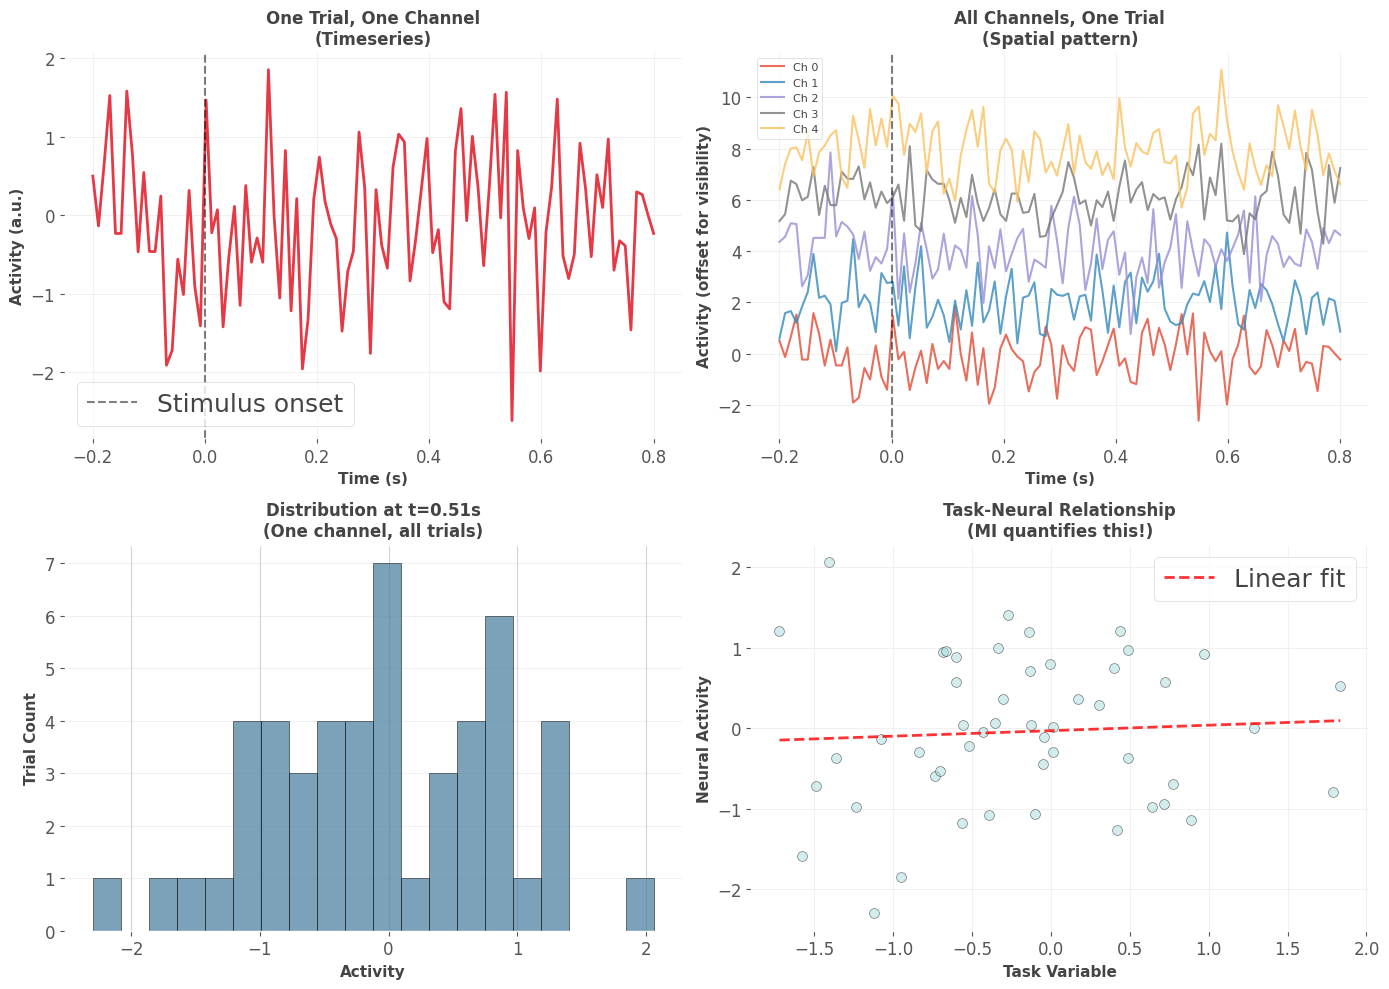
\includegraphics[keepaspectratio]{04_frites_neural_timeseries_files/figure-pdf/cell-5-output-1.png}}

\begin{verbatim}

📊 Understanding the Data Structure:
============================================================
Top-left: How activity evolves in time (temporal dynamics)
Top-right: How channels relate at one moment (spatial pattern)
Bottom-left: Trial-to-trial variability (what MI uses!)
Bottom-right: Task-neural relationship (what MI measures)

💡 Frites computes MI at each time point using trial variability
\end{verbatim}

\section{Part 2: Time-Resolved Mutual
Information}\label{part-2-time-resolved-mutual-information}

\subsection{The Core Workflow: WfMi}\label{the-core-workflow-wfmi}

Frites organizes analysis into \textbf{workflows}. The main one for
mutual information is \texttt{WfMi} (Workflow for Mutual Information).
Here's how it works:

\begin{Shaded}
\begin{Highlighting}[]
\NormalTok{wf }\OperatorTok{=}\NormalTok{ WfMi(}
\NormalTok{    mi\_type}\OperatorTok{=}\StringTok{\textquotesingle{}cd\textquotesingle{}}\NormalTok{,     }\CommentTok{\# \textquotesingle{}cd\textquotesingle{} = continuous{-}discrete (neural vs condition)}
                      \CommentTok{\# \textquotesingle{}cc\textquotesingle{} = continuous{-}continuous (neural vs neural or behavior)}
                      \CommentTok{\# \textquotesingle{}ccd\textquotesingle{} = continuous{-}continuous|discrete (conditional MI)}
\NormalTok{    inference}\OperatorTok{=}\StringTok{\textquotesingle{}ffx\textquotesingle{}}   \CommentTok{\# \textquotesingle{}ffx\textquotesingle{} = fixed{-}effect (pool across subjects)}
                      \CommentTok{\# \textquotesingle{}rfx\textquotesingle{} = random{-}effect (model inter{-}subject variability)}
\NormalTok{)}
\end{Highlighting}
\end{Shaded}

\subsection{Gaussian Copula MI (GCMI)}\label{gaussian-copula-mi-gcmi}

Frites uses \textbf{GCMI} by default. This is important to understand:

\textbf{What it does}: Transforms data to have Gaussian marginals while
preserving rank relationships.

\textbf{Why it's good}: - No binning required (unlike histograms) - Fast
computation - Works for any monotonic relationship - Accurate with
modest sample sizes

\textbf{Key assumption}: The relationship is \textbf{monotonic} (if X
increases, Y consistently increases OR decreases, not both)

\textbf{When it fails}: Non-monotonic relationships (rare in neural
data)

Let's create data with a clear time-resolved effect and analyze it:

\begin{Shaded}
\begin{Highlighting}[]
\KeywordTok{def}\NormalTok{ simulate\_task\_related\_activity(n\_subjects}\OperatorTok{=}\DecValTok{3}\NormalTok{, n\_epochs}\OperatorTok{=}\DecValTok{80}\NormalTok{, n\_channels}\OperatorTok{=}\DecValTok{8}\NormalTok{, n\_times}\OperatorTok{=}\DecValTok{150}\NormalTok{):}
    \CommentTok{"""}
\CommentTok{    Simulate neural data with task{-}related MI in specific time window.}
\CommentTok{    }
\CommentTok{    Task variable affects neural activity at 400{-}600ms.}
\CommentTok{    """}
\NormalTok{    time }\OperatorTok{=}\NormalTok{ np.linspace(}\OperatorTok{{-}}\FloatTok{0.2}\NormalTok{, }\FloatTok{1.0}\NormalTok{, n\_times)}
    
\NormalTok{    data\_list }\OperatorTok{=}\NormalTok{ []}
\NormalTok{    y\_list }\OperatorTok{=}\NormalTok{ []}
\NormalTok{    roi\_list }\OperatorTok{=}\NormalTok{ []}
    
    \ControlFlowTok{for}\NormalTok{ subj }\KeywordTok{in} \BuiltInTok{range}\NormalTok{(n\_subjects):}
        \CommentTok{\# Each subject has slightly different trial count}
\NormalTok{        n\_epochs\_subj }\OperatorTok{=}\NormalTok{ n\_epochs }\OperatorTok{+}\NormalTok{ np.random.randint(}\OperatorTok{{-}}\DecValTok{10}\NormalTok{, }\DecValTok{10}\NormalTok{)}
        
        \CommentTok{\# Neural data}
\NormalTok{        subj\_data }\OperatorTok{=}\NormalTok{ np.random.randn(n\_epochs\_subj, n\_channels, n\_times) }\OperatorTok{*} \FloatTok{0.5}
        
        \CommentTok{\# Task variable (continuous)}
\NormalTok{        task\_var }\OperatorTok{=}\NormalTok{ np.random.randn(n\_epochs\_subj)}
        
        \CommentTok{\# Inject MI in specific channels and time window}
        \CommentTok{\# Channels 2{-}4 encode task in 400{-}600ms window}
\NormalTok{        task\_time\_mask }\OperatorTok{=}\NormalTok{ (time }\OperatorTok{\textgreater{}=} \FloatTok{0.4}\NormalTok{) }\OperatorTok{\&}\NormalTok{ (time }\OperatorTok{\textless{}=} \FloatTok{0.6}\NormalTok{)}
\NormalTok{        task\_channels }\OperatorTok{=}\NormalTok{ [}\DecValTok{2}\NormalTok{, }\DecValTok{3}\NormalTok{, }\DecValTok{4}\NormalTok{]}
        
        \ControlFlowTok{for}\NormalTok{ ch }\KeywordTok{in}\NormalTok{ task\_channels:}
            \CommentTok{\# Add task{-}related modulation}
\NormalTok{            subj\_data[:, ch, task\_time\_mask] }\OperatorTok{+=}\NormalTok{ task\_var[:, np.newaxis] }\OperatorTok{*} \FloatTok{1.5}
        
        \CommentTok{\# Add smooth temporal dynamics (autocorrelation)}
        \ImportTok{from}\NormalTok{ scipy.ndimage }\ImportTok{import}\NormalTok{ gaussian\_filter1d}
        \ControlFlowTok{for}\NormalTok{ ep }\KeywordTok{in} \BuiltInTok{range}\NormalTok{(n\_epochs\_subj):}
            \ControlFlowTok{for}\NormalTok{ ch }\KeywordTok{in} \BuiltInTok{range}\NormalTok{(n\_channels):}
\NormalTok{                subj\_data[ep, ch, :] }\OperatorTok{=}\NormalTok{ gaussian\_filter1d(subj\_data[ep, ch, :], sigma}\OperatorTok{=}\DecValTok{2}\NormalTok{)}
        
\NormalTok{        data\_list.append(subj\_data)}
\NormalTok{        y\_list.append(task\_var)}
\NormalTok{        roi\_list.append([}\SpecialStringTok{f\textquotesingle{}CH\_}\SpecialCharTok{\{}\NormalTok{i}\SpecialCharTok{\}}\SpecialStringTok{\textquotesingle{}} \ControlFlowTok{for}\NormalTok{ i }\KeywordTok{in} \BuiltInTok{range}\NormalTok{(n\_channels)])}
    
    \ControlFlowTok{return}\NormalTok{ data\_list, y\_list, roi\_list, time}

\CommentTok{\# Generate data}
\NormalTok{data, task\_vars, rois, time }\OperatorTok{=}\NormalTok{ simulate\_task\_related\_activity()}

\BuiltInTok{print}\NormalTok{(}\StringTok{"Simulated Task{-}Related Activity"}\NormalTok{)}
\BuiltInTok{print}\NormalTok{(}\StringTok{"="} \OperatorTok{*} \DecValTok{60}\NormalTok{)}
\BuiltInTok{print}\NormalTok{(}\SpecialStringTok{f"Subjects: }\SpecialCharTok{\{}\BuiltInTok{len}\NormalTok{(data)}\SpecialCharTok{\}}\SpecialStringTok{"}\NormalTok{)}
\BuiltInTok{print}\NormalTok{(}\SpecialStringTok{f"Channels: }\SpecialCharTok{\{}\BuiltInTok{len}\NormalTok{(rois[}\DecValTok{0}\NormalTok{])}\SpecialCharTok{\}}\SpecialStringTok{"}\NormalTok{)}
\BuiltInTok{print}\NormalTok{(}\SpecialStringTok{f"Time points: }\SpecialCharTok{\{}\BuiltInTok{len}\NormalTok{(time)}\SpecialCharTok{\}}\SpecialStringTok{"}\NormalTok{)}
\BuiltInTok{print}\NormalTok{(}\SpecialStringTok{f"Time range: }\SpecialCharTok{\{}\NormalTok{time[}\DecValTok{0}\NormalTok{]}\SpecialCharTok{:.2f\}}\SpecialStringTok{s to }\SpecialCharTok{\{}\NormalTok{time[}\OperatorTok{{-}}\DecValTok{1}\NormalTok{]}\SpecialCharTok{:.2f\}}\SpecialStringTok{s"}\NormalTok{)}
\BuiltInTok{print}\NormalTok{(}\SpecialStringTok{f"}\CharTok{\textbackslash{}n}\SpecialStringTok{Trials per subject: }\SpecialCharTok{\{}\NormalTok{[d.shape[}\DecValTok{0}\NormalTok{] }\ControlFlowTok{for}\NormalTok{ d }\KeywordTok{in}\NormalTok{ data]}\SpecialCharTok{\}}\SpecialStringTok{"}\NormalTok{)}
\BuiltInTok{print}\NormalTok{(}\StringTok{"}\CharTok{\textbackslash{}n}\StringTok{✨ Ground Truth:"}\NormalTok{)}
\BuiltInTok{print}\NormalTok{(}\StringTok{"   Channels 2, 3, 4 encode task variable"}\NormalTok{)}
\BuiltInTok{print}\NormalTok{(}\StringTok{"   Time window: 400{-}600ms post{-}stimulus"}\NormalTok{)}
\BuiltInTok{print}\NormalTok{(}\StringTok{"   Let\textquotesingle{}s see if Frites can detect this!"}\NormalTok{)}

\CommentTok{\# Create DatasetEphy}
\NormalTok{ds }\OperatorTok{=}\NormalTok{ DatasetEphy(x}\OperatorTok{=}\NormalTok{data, y}\OperatorTok{=}\NormalTok{task\_vars, roi}\OperatorTok{=}\NormalTok{rois, times}\OperatorTok{=}\NormalTok{time)}

\BuiltInTok{print}\NormalTok{(}\StringTok{"}\CharTok{\textbackslash{}n}\StringTok{"} \OperatorTok{+} \StringTok{"="} \OperatorTok{*} \DecValTok{60}\NormalTok{)}
\BuiltInTok{print}\NormalTok{(}\StringTok{"Dataset ready for analysis!"}\NormalTok{)}
\BuiltInTok{print}\NormalTok{(}\StringTok{"="} \OperatorTok{*} \DecValTok{60}\NormalTok{)}
\end{Highlighting}
\end{Shaded}

\begin{verbatim}
Simulated Task-Related Activity
============================================================
Subjects: 3
Channels: 8
Time points: 150
Time range: -0.20s to 1.00s

Trials per subject: [71, 72, 83]

✨ Ground Truth:
   Channels 2, 3, 4 encode task variable
   Time window: 400-600ms post-stimulus
   Let's see if Frites can detect this!

============================================================
Dataset ready for analysis!
============================================================
\end{verbatim}

\subsection{Computing Time-Resolved
MI}\label{computing-time-resolved-mi}

Now we'll use the \texttt{WfMi} workflow to compute mutual information
at each time point. We'll also apply \textbf{permutation testing} to
determine statistical significance.

\subsubsection{How Permutation Testing
Works}\label{how-permutation-testing-works}

\begin{enumerate}
\def\labelenumi{\arabic{enumi}.}
\tightlist
\item
  Compute real MI from actual data
\item
  Shuffle trial labels randomly (breaking task-neural relationship)
\item
  Compute MI on shuffled data
\item
  Repeat 1000+ times to build null distribution
\item
  Compare real MI to null: p-value = proportion of shuffles with higher
  MI
\end{enumerate}

This tests: ``Could this MI value occur by chance?''

\begin{Shaded}
\begin{Highlighting}[]
\CommentTok{\# Define workflow}
\NormalTok{wf }\OperatorTok{=}\NormalTok{ WfMi(}
\NormalTok{    mi\_type}\OperatorTok{=}\StringTok{\textquotesingle{}cc\textquotesingle{}}\NormalTok{,      }\CommentTok{\# continuous{-}continuous (neural activity vs task variable)}
\NormalTok{    inference}\OperatorTok{=}\StringTok{\textquotesingle{}ffx\textquotesingle{}}\NormalTok{,   }\CommentTok{\# fixed{-}effect (pool data across subjects)}
\NormalTok{    verbose}\OperatorTok{=}\VariableTok{True}       \CommentTok{\# Show progress}
\NormalTok{)}

\BuiltInTok{print}\NormalTok{(}\StringTok{"Computing Time{-}Resolved MI..."}\NormalTok{)}
\BuiltInTok{print}\NormalTok{(}\StringTok{"This will:"}\NormalTok{)}
\BuiltInTok{print}\NormalTok{(}\StringTok{"  1. Compute MI at each time point"}\NormalTok{)}
\BuiltInTok{print}\NormalTok{(}\StringTok{"  2. Run 200 permutations for significance testing"}\NormalTok{)}
\BuiltInTok{print}\NormalTok{(}\StringTok{"  3. Apply cluster{-}based correction"}\NormalTok{)}
\BuiltInTok{print}\NormalTok{(}\StringTok{"}\CharTok{\textbackslash{}n}\StringTok{Progress:"}\NormalTok{)}

\CommentTok{\# Compute MI with statistical testing}
\NormalTok{mi, pvalues }\OperatorTok{=}\NormalTok{ wf.fit(}
\NormalTok{    ds,}
\NormalTok{    n\_perm}\OperatorTok{=}\DecValTok{200}\NormalTok{,         }\CommentTok{\# Number of permutations (use 1000+ for publication)}
\NormalTok{    mcp}\OperatorTok{=}\StringTok{\textquotesingle{}cluster\textquotesingle{}}\NormalTok{,      }\CommentTok{\# Multiple comparison correction method}
\NormalTok{    cluster\_th}\OperatorTok{=}\VariableTok{None}\NormalTok{,    }\CommentTok{\# Automatically determine threshold}
\NormalTok{    random\_state}\OperatorTok{=}\DecValTok{42}\NormalTok{,}
\NormalTok{    n\_jobs}\OperatorTok{=}\DecValTok{1}            \CommentTok{\# Parallel jobs (use {-}1 for all cores)}
\NormalTok{)}

\BuiltInTok{print}\NormalTok{(}\StringTok{"}\CharTok{\textbackslash{}n}\StringTok{✓ Computation complete!"}\NormalTok{)}
\BuiltInTok{print}\NormalTok{(}\SpecialStringTok{f"}\CharTok{\textbackslash{}n}\SpecialStringTok{Results shapes:"}\NormalTok{)}
\BuiltInTok{print}\NormalTok{(}\SpecialStringTok{f"  MI: }\SpecialCharTok{\{}\NormalTok{mi}\SpecialCharTok{.}\NormalTok{shape}\SpecialCharTok{\}}\SpecialStringTok{"}\NormalTok{)}
\BuiltInTok{print}\NormalTok{(}\SpecialStringTok{f"  P{-}values: }\SpecialCharTok{\{}\NormalTok{pvalues}\SpecialCharTok{.}\NormalTok{shape}\SpecialCharTok{\}}\SpecialStringTok{"}\NormalTok{)}
\BuiltInTok{print}\NormalTok{(}\SpecialStringTok{f"}\CharTok{\textbackslash{}n}\SpecialStringTok{Results are xarray DataArrays with labeled dimensions:"}\NormalTok{)}
\BuiltInTok{print}\NormalTok{(}\SpecialStringTok{f"  Dimensions: }\SpecialCharTok{\{}\BuiltInTok{list}\NormalTok{(mi.dims)}\SpecialCharTok{\}}\SpecialStringTok{"}\NormalTok{)}
\BuiltInTok{print}\NormalTok{(}\SpecialStringTok{f"  Coordinates: }\SpecialCharTok{\{}\BuiltInTok{list}\NormalTok{(mi.coords.keys())}\SpecialCharTok{\}}\SpecialStringTok{"}\NormalTok{)}
\end{Highlighting}
\end{Shaded}

\begin{verbatim}
Computing Time-Resolved MI...
This will:
  1. Compute MI at each time point
  2. Run 200 permutations for significance testing
  3. Apply cluster-based correction

Progress:
\end{verbatim}

\begin{verbatim}

✓ Computation complete!

Results shapes:
  MI: (150, 8)
  P-values: (150, 8)

Results are xarray DataArrays with labeled dimensions:
  Dimensions: ['times', 'roi']
  Coordinates: ['times', 'roi']
\end{verbatim}

\subsection{Visualizing Time-Resolved MI
Results}\label{visualizing-time-resolved-mi-results}

The beauty of Frites is that results come as \texttt{xarray} DataArrays,
which have built-in plotting and labeled dimensions. Let's visualize the
results:

\begin{Shaded}
\begin{Highlighting}[]
\CommentTok{\# Plot MI and p{-}values for all channels}
\NormalTok{fig, axes }\OperatorTok{=}\NormalTok{ plt.subplots(}\DecValTok{2}\NormalTok{, }\DecValTok{1}\NormalTok{, figsize}\OperatorTok{=}\NormalTok{(}\DecValTok{14}\NormalTok{, }\DecValTok{10}\NormalTok{))}

\CommentTok{\# Top panel: MI timecourses}
\NormalTok{ax1 }\OperatorTok{=}\NormalTok{ axes[}\DecValTok{0}\NormalTok{]}
\ControlFlowTok{for}\NormalTok{ ch }\KeywordTok{in} \BuiltInTok{range}\NormalTok{(}\BuiltInTok{len}\NormalTok{(rois[}\DecValTok{0}\NormalTok{])):}
\NormalTok{    roi\_name }\OperatorTok{=}\NormalTok{ rois[}\DecValTok{0}\NormalTok{][ch]}
\NormalTok{    mi\_ch }\OperatorTok{=}\NormalTok{ mi.sel(roi}\OperatorTok{=}\NormalTok{roi\_name).squeeze()}
    
    \CommentTok{\# Highlight task{-}encoding channels}
    \ControlFlowTok{if}\NormalTok{ ch }\KeywordTok{in}\NormalTok{ [}\DecValTok{2}\NormalTok{, }\DecValTok{3}\NormalTok{, }\DecValTok{4}\NormalTok{]:}
\NormalTok{        ax1.plot(time, mi\_ch, linewidth}\OperatorTok{=}\DecValTok{3}\NormalTok{, label}\OperatorTok{=}\NormalTok{roi\_name, alpha}\OperatorTok{=}\FloatTok{0.9}\NormalTok{)}
    \ControlFlowTok{else}\NormalTok{:}
\NormalTok{        ax1.plot(time, mi\_ch, linewidth}\OperatorTok{=}\FloatTok{1.5}\NormalTok{, alpha}\OperatorTok{=}\FloatTok{0.5}\NormalTok{, color}\OperatorTok{=}\StringTok{\textquotesingle{}gray\textquotesingle{}}\NormalTok{)}

\NormalTok{ax1.axvline(}\DecValTok{0}\NormalTok{, color}\OperatorTok{=}\StringTok{\textquotesingle{}k\textquotesingle{}}\NormalTok{, linestyle}\OperatorTok{=}\StringTok{\textquotesingle{}{-}{-}\textquotesingle{}}\NormalTok{, linewidth}\OperatorTok{=}\DecValTok{2}\NormalTok{, alpha}\OperatorTok{=}\FloatTok{0.7}\NormalTok{, label}\OperatorTok{=}\StringTok{\textquotesingle{}Stimulus\textquotesingle{}}\NormalTok{)}
\NormalTok{ax1.axvspan(}\FloatTok{0.4}\NormalTok{, }\FloatTok{0.6}\NormalTok{, alpha}\OperatorTok{=}\FloatTok{0.2}\NormalTok{, color}\OperatorTok{=}\StringTok{\textquotesingle{}red\textquotesingle{}}\NormalTok{, label}\OperatorTok{=}\StringTok{\textquotesingle{}Injected MI window\textquotesingle{}}\NormalTok{)}
\NormalTok{ax1.axhline(}\DecValTok{0}\NormalTok{, color}\OperatorTok{=}\StringTok{\textquotesingle{}k\textquotesingle{}}\NormalTok{, linestyle}\OperatorTok{=}\StringTok{\textquotesingle{}{-}\textquotesingle{}}\NormalTok{, linewidth}\OperatorTok{=}\DecValTok{1}\NormalTok{, alpha}\OperatorTok{=}\FloatTok{0.3}\NormalTok{)}
\NormalTok{ax1.set\_xlabel(}\StringTok{\textquotesingle{}Time (s)\textquotesingle{}}\NormalTok{, fontsize}\OperatorTok{=}\DecValTok{13}\NormalTok{, fontweight}\OperatorTok{=}\StringTok{\textquotesingle{}bold\textquotesingle{}}\NormalTok{)}
\NormalTok{ax1.set\_ylabel(}\StringTok{\textquotesingle{}Mutual Information (bits)\textquotesingle{}}\NormalTok{, fontsize}\OperatorTok{=}\DecValTok{13}\NormalTok{, fontweight}\OperatorTok{=}\StringTok{\textquotesingle{}bold\textquotesingle{}}\NormalTok{)}
\NormalTok{ax1.set\_title(}\StringTok{\textquotesingle{}Time{-}Resolved MI: Task Variable vs Neural Activity\textquotesingle{}}\NormalTok{, }
\NormalTok{              fontsize}\OperatorTok{=}\DecValTok{14}\NormalTok{, fontweight}\OperatorTok{=}\StringTok{\textquotesingle{}bold\textquotesingle{}}\NormalTok{)}
\NormalTok{ax1.legend(loc}\OperatorTok{=}\StringTok{\textquotesingle{}upper left\textquotesingle{}}\NormalTok{, fontsize}\OperatorTok{=}\DecValTok{9}\NormalTok{, ncol}\OperatorTok{=}\DecValTok{2}\NormalTok{)}
\NormalTok{ax1.grid(}\VariableTok{True}\NormalTok{, alpha}\OperatorTok{=}\FloatTok{0.3}\NormalTok{)}

\CommentTok{\# Bottom panel: P{-}values (focus on task{-}encoding channels)}
\NormalTok{ax2 }\OperatorTok{=}\NormalTok{ axes[}\DecValTok{1}\NormalTok{]}
\ControlFlowTok{for}\NormalTok{ ch }\KeywordTok{in}\NormalTok{ [}\DecValTok{2}\NormalTok{, }\DecValTok{3}\NormalTok{, }\DecValTok{4}\NormalTok{]:}
\NormalTok{    roi\_name }\OperatorTok{=}\NormalTok{ rois[}\DecValTok{0}\NormalTok{][ch]}
\NormalTok{    pv\_ch }\OperatorTok{=}\NormalTok{ pvalues.sel(roi}\OperatorTok{=}\NormalTok{roi\_name).squeeze()}
    
    \CommentTok{\# Mask non{-}significant}
\NormalTok{    pv\_sig }\OperatorTok{=}\NormalTok{ pv\_ch.copy()}
\NormalTok{    pv\_sig }\OperatorTok{=}\NormalTok{ pv\_sig.where(pv\_sig }\OperatorTok{\textless{}} \FloatTok{0.05}\NormalTok{)}
    
\NormalTok{    ax2.plot(time, pv\_ch, linewidth}\OperatorTok{=}\FloatTok{1.5}\NormalTok{, alpha}\OperatorTok{=}\FloatTok{0.4}\NormalTok{, color}\OperatorTok{=}\StringTok{\textquotesingle{}gray\textquotesingle{}}\NormalTok{)}
\NormalTok{    ax2.plot(time, pv\_sig, linewidth}\OperatorTok{=}\DecValTok{3}\NormalTok{, label}\OperatorTok{=}\NormalTok{roi\_name)}

\NormalTok{ax2.axhline(}\FloatTok{0.05}\NormalTok{, color}\OperatorTok{=}\StringTok{\textquotesingle{}red\textquotesingle{}}\NormalTok{, linestyle}\OperatorTok{=}\StringTok{\textquotesingle{}{-}{-}\textquotesingle{}}\NormalTok{, linewidth}\OperatorTok{=}\DecValTok{2}\NormalTok{, label}\OperatorTok{=}\StringTok{\textquotesingle{}α = 0.05\textquotesingle{}}\NormalTok{)}
\NormalTok{ax2.axvspan(}\FloatTok{0.4}\NormalTok{, }\FloatTok{0.6}\NormalTok{, alpha}\OperatorTok{=}\FloatTok{0.2}\NormalTok{, color}\OperatorTok{=}\StringTok{\textquotesingle{}red\textquotesingle{}}\NormalTok{)}
\NormalTok{ax2.set\_xlabel(}\StringTok{\textquotesingle{}Time (s)\textquotesingle{}}\NormalTok{, fontsize}\OperatorTok{=}\DecValTok{13}\NormalTok{, fontweight}\OperatorTok{=}\StringTok{\textquotesingle{}bold\textquotesingle{}}\NormalTok{)}
\NormalTok{ax2.set\_ylabel(}\StringTok{\textquotesingle{}P{-}value\textquotesingle{}}\NormalTok{, fontsize}\OperatorTok{=}\DecValTok{13}\NormalTok{, fontweight}\OperatorTok{=}\StringTok{\textquotesingle{}bold\textquotesingle{}}\NormalTok{)}
\NormalTok{ax2.set\_title(}\StringTok{\textquotesingle{}Statistical Significance (cluster{-}corrected)\textquotesingle{}}\NormalTok{, fontsize}\OperatorTok{=}\DecValTok{14}\NormalTok{, fontweight}\OperatorTok{=}\StringTok{\textquotesingle{}bold\textquotesingle{}}\NormalTok{)}
\NormalTok{ax2.set\_yscale(}\StringTok{\textquotesingle{}log\textquotesingle{}}\NormalTok{)}
\NormalTok{ax2.legend(loc}\OperatorTok{=}\StringTok{\textquotesingle{}upper left\textquotesingle{}}\NormalTok{, fontsize}\OperatorTok{=}\DecValTok{10}\NormalTok{)}
\NormalTok{ax2.grid(}\VariableTok{True}\NormalTok{, alpha}\OperatorTok{=}\FloatTok{0.3}\NormalTok{)}
\NormalTok{ax2.set\_ylim([}\FloatTok{1e{-}4}\NormalTok{, }\DecValTok{1}\NormalTok{])}

\NormalTok{plt.tight\_layout()}
\NormalTok{plt.show()}

\BuiltInTok{print}\NormalTok{(}\StringTok{"}\CharTok{\textbackslash{}n}\StringTok{🎯 Analysis Results:"}\NormalTok{)}
\BuiltInTok{print}\NormalTok{(}\StringTok{"="} \OperatorTok{*} \DecValTok{60}\NormalTok{)}

\CommentTok{\# Check detection of ground truth}
\ControlFlowTok{for}\NormalTok{ ch }\KeywordTok{in}\NormalTok{ [}\DecValTok{2}\NormalTok{, }\DecValTok{3}\NormalTok{, }\DecValTok{4}\NormalTok{]:}
\NormalTok{    roi\_name }\OperatorTok{=}\NormalTok{ rois[}\DecValTok{0}\NormalTok{][ch]}
\NormalTok{    pv\_ch }\OperatorTok{=}\NormalTok{ pvalues.sel(roi}\OperatorTok{=}\NormalTok{roi\_name).squeeze()}
    
    \CommentTok{\# Find significant time windows}
\NormalTok{    sig\_times }\OperatorTok{=}\NormalTok{ time[pv\_ch.values }\OperatorTok{\textless{}} \FloatTok{0.05}\NormalTok{]}
    
    \ControlFlowTok{if} \BuiltInTok{len}\NormalTok{(sig\_times) }\OperatorTok{\textgreater{}} \DecValTok{0}\NormalTok{:}
        \BuiltInTok{print}\NormalTok{(}\SpecialStringTok{f"}\CharTok{\textbackslash{}n}\SpecialCharTok{\{}\NormalTok{roi\_name}\SpecialCharTok{\}}\SpecialStringTok{:"}\NormalTok{)}
        \BuiltInTok{print}\NormalTok{(}\SpecialStringTok{f"  ✓ Significant MI detected"}\NormalTok{)}
        \BuiltInTok{print}\NormalTok{(}\SpecialStringTok{f"  Time range: }\SpecialCharTok{\{}\NormalTok{sig\_times[}\DecValTok{0}\NormalTok{]}\SpecialCharTok{:.2f\}}\SpecialStringTok{s to }\SpecialCharTok{\{}\NormalTok{sig\_times[}\OperatorTok{{-}}\DecValTok{1}\NormalTok{]}\SpecialCharTok{:.2f\}}\SpecialStringTok{s"}\NormalTok{)}
        \BuiltInTok{print}\NormalTok{(}\SpecialStringTok{f"  Peak MI: }\SpecialCharTok{\{}\NormalTok{mi}\SpecialCharTok{.}\NormalTok{sel(roi}\OperatorTok{=}\NormalTok{roi\_name)}\SpecialCharTok{.}\BuiltInTok{max}\NormalTok{()}\SpecialCharTok{.}\NormalTok{values}\SpecialCharTok{:.4f\}}\SpecialStringTok{ bits"}\NormalTok{)}
        
        \CommentTok{\# Check if this overlaps with ground truth (400{-}600ms)}
\NormalTok{        overlap }\OperatorTok{=}\NormalTok{ (sig\_times }\OperatorTok{\textgreater{}=} \FloatTok{0.4}\NormalTok{) }\OperatorTok{\&}\NormalTok{ (sig\_times }\OperatorTok{\textless{}=} \FloatTok{0.6}\NormalTok{)}
        \ControlFlowTok{if}\NormalTok{ overlap.}\BuiltInTok{any}\NormalTok{():}
            \BuiltInTok{print}\NormalTok{(}\SpecialStringTok{f"  ✨ Correctly detected ground truth window!"}\NormalTok{)}
    \ControlFlowTok{else}\NormalTok{:}
        \BuiltInTok{print}\NormalTok{(}\SpecialStringTok{f"}\CharTok{\textbackslash{}n}\SpecialCharTok{\{}\NormalTok{roi\_name}\SpecialCharTok{\}}\SpecialStringTok{: No significant MI detected"}\NormalTok{)}

\BuiltInTok{print}\NormalTok{(}\StringTok{"}\CharTok{\textbackslash{}n}\StringTok{"} \OperatorTok{+} \StringTok{"="} \OperatorTok{*} \DecValTok{60}\NormalTok{)}
\BuiltInTok{print}\NormalTok{(}\StringTok{"}\CharTok{\textbackslash{}n}\StringTok{💡 Key Insight: Frites successfully detected the injected MI!"}\NormalTok{)}
\BuiltInTok{print}\NormalTok{(}\StringTok{"   Statistical testing confirmed it\textquotesingle{}s not due to chance."}\NormalTok{)}
\end{Highlighting}
\end{Shaded}

\pandocbounded{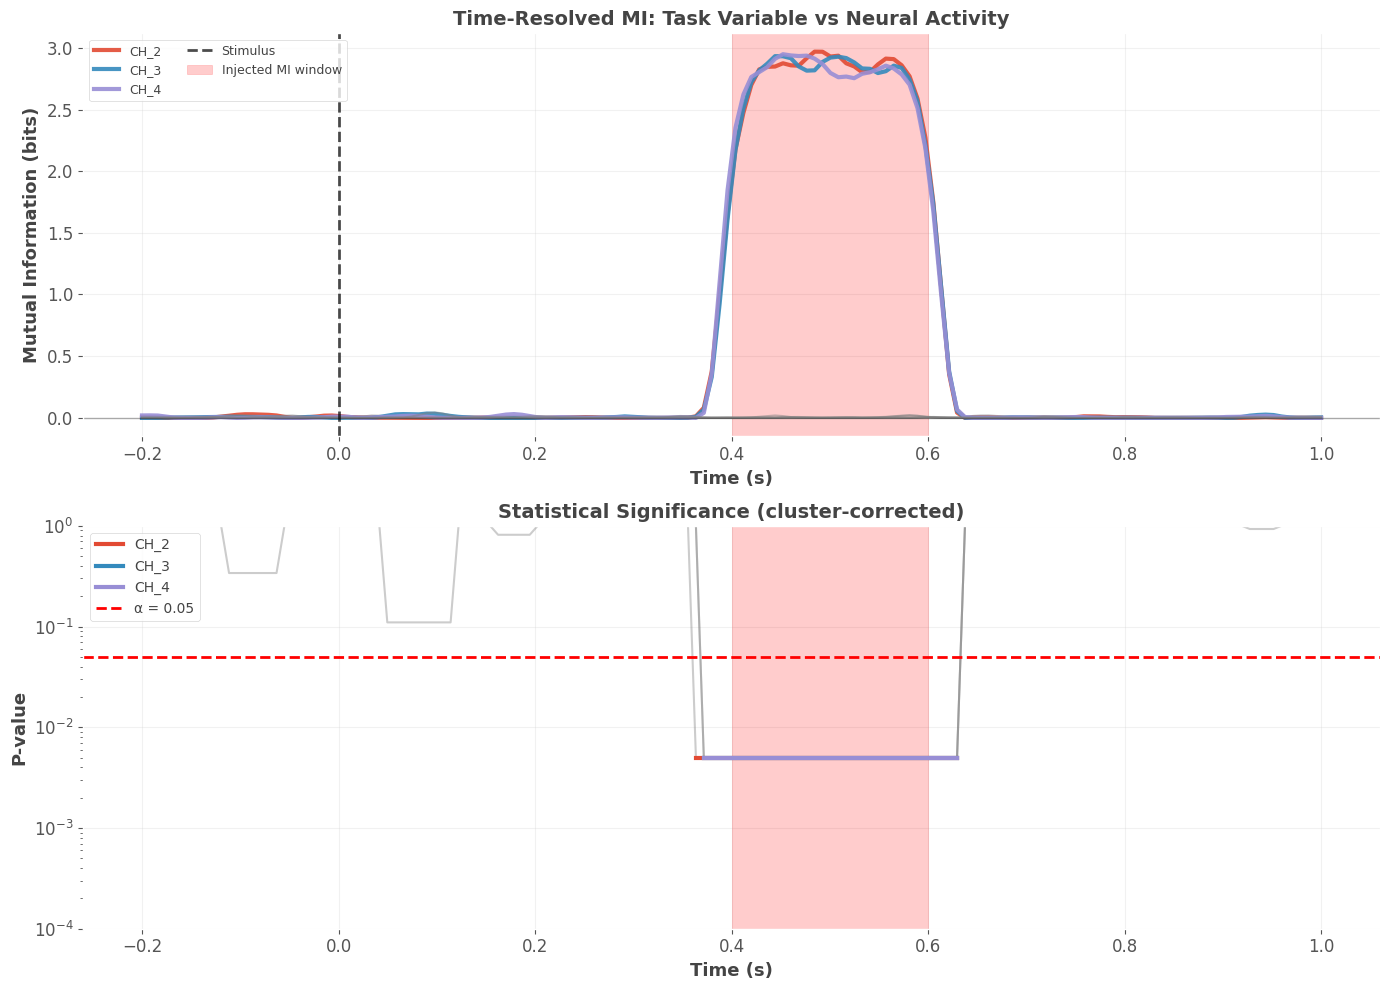
\includegraphics[keepaspectratio]{04_frites_neural_timeseries_files/figure-pdf/cell-8-output-1.png}}

\begin{verbatim}

🎯 Analysis Results:
============================================================

CH_2:
  ✓ Significant MI detected
  Time range: 0.36s to 0.63s
  Peak MI: 2.9730 bits
  ✨ Correctly detected ground truth window!

CH_3:
  ✓ Significant MI detected
  Time range: 0.37s to 0.63s
  Peak MI: 2.9363 bits
  ✨ Correctly detected ground truth window!

CH_4:
  ✓ Significant MI detected
  Time range: 0.37s to 0.63s
  Peak MI: 2.9521 bits
  ✨ Correctly detected ground truth window!

============================================================

💡 Key Insight: Frites successfully detected the injected MI!
   Statistical testing confirmed it's not due to chance.
\end{verbatim}

\section{Part 3: Understanding Multiple Comparison
Correction}\label{part-3-understanding-multiple-comparison-correction}

\subsection{The Multiple Comparison
Problem}\label{the-multiple-comparison-problem}

When you compute MI at 100 time points, you're doing 100 statistical
tests. If you use α = 0.05 for each test: - Expected false positives:
100 × 0.05 = 5 - Even with pure noise, you'd see \textasciitilde5
``significant'' time points!

This is the \textbf{multiple comparisons problem}, and it's critical to
address.

\subsection{Correction Methods in
Frites}\label{correction-methods-in-frites}

Frites provides several correction methods (via \texttt{mcp} parameter):

\begin{enumerate}
\def\labelenumi{\arabic{enumi}.}
\tightlist
\item
  \textbf{`cluster'} (default): Cluster-based permutation testing

  \begin{itemize}
  \tightlist
  \item
    Finds contiguous significant time points (clusters)
  \item
    Tests if cluster size exceeds chance
  \item
    Controls family-wise error rate (FWER)
  \item
    \textbf{Best for}: Time series with expected temporal contiguity
  \end{itemize}
\item
  \textbf{`maxstat'}: Maximum statistic

  \begin{itemize}
  \tightlist
  \item
    Tests against maximum MI across all time points in permutations
  \item
    Very conservative
  \item
    \textbf{Best for}: Hypothesis about peak effect
  \end{itemize}
\item
  \textbf{`fdr'}: False Discovery Rate

  \begin{itemize}
  \tightlist
  \item
    Controls proportion of false positives
  \item
    Less conservative than FWER
  \item
    \textbf{Best for}: Exploratory analyses
  \end{itemize}
\item
  \textbf{`bonferroni'}: Bonferroni correction

  \begin{itemize}
  \tightlist
  \item
    Divides α by number of tests
  \item
    Very conservative
  \item
    \textbf{Best for}: Few planned comparisons
  \end{itemize}
\end{enumerate}

Let's compare these methods on the same data:

\begin{Shaded}
\begin{Highlighting}[]
\CommentTok{\# Compare different MCP methods}
\NormalTok{mcp\_methods }\OperatorTok{=}\NormalTok{ [}\StringTok{\textquotesingle{}cluster\textquotesingle{}}\NormalTok{, }\StringTok{\textquotesingle{}maxstat\textquotesingle{}}\NormalTok{, }\StringTok{\textquotesingle{}fdr\textquotesingle{}}\NormalTok{, }\StringTok{\textquotesingle{}bonferroni\textquotesingle{}}\NormalTok{]}
\NormalTok{results }\OperatorTok{=}\NormalTok{ \{\}}

\BuiltInTok{print}\NormalTok{(}\StringTok{"Comparing Multiple Comparison Corrections"}\NormalTok{)}
\BuiltInTok{print}\NormalTok{(}\StringTok{"="} \OperatorTok{*} \DecValTok{60}\NormalTok{)}
\BuiltInTok{print}\NormalTok{(}\StringTok{"Computing MI with different corrections...}\CharTok{\textbackslash{}n}\StringTok{"}\NormalTok{)}

\ControlFlowTok{for}\NormalTok{ mcp }\KeywordTok{in}\NormalTok{ mcp\_methods:}
    \BuiltInTok{print}\NormalTok{(}\SpecialStringTok{f"Running }\SpecialCharTok{\{}\NormalTok{mcp}\SpecialCharTok{\}}\SpecialStringTok{..."}\NormalTok{)}
\NormalTok{    wf }\OperatorTok{=}\NormalTok{ WfMi(mi\_type}\OperatorTok{=}\StringTok{\textquotesingle{}cc\textquotesingle{}}\NormalTok{, inference}\OperatorTok{=}\StringTok{\textquotesingle{}ffx\textquotesingle{}}\NormalTok{, verbose}\OperatorTok{=}\VariableTok{False}\NormalTok{)}
\NormalTok{    mi\_mcp, pv\_mcp }\OperatorTok{=}\NormalTok{ wf.fit(ds, n\_perm}\OperatorTok{=}\DecValTok{200}\NormalTok{, mcp}\OperatorTok{=}\NormalTok{mcp, random\_state}\OperatorTok{=}\DecValTok{42}\NormalTok{, n\_jobs}\OperatorTok{=}\DecValTok{1}\NormalTok{)}
\NormalTok{    results[mcp] }\OperatorTok{=}\NormalTok{ \{}\StringTok{\textquotesingle{}mi\textquotesingle{}}\NormalTok{: mi\_mcp, }\StringTok{\textquotesingle{}pv\textquotesingle{}}\NormalTok{: pv\_mcp\}}

\BuiltInTok{print}\NormalTok{(}\StringTok{"}\CharTok{\textbackslash{}n}\StringTok{Done! Plotting comparison..."}\NormalTok{)}

\CommentTok{\# Visualize comparison for Channel 3 (task{-}encoding)}
\NormalTok{fig, axes }\OperatorTok{=}\NormalTok{ plt.subplots(}\BuiltInTok{len}\NormalTok{(mcp\_methods), }\DecValTok{1}\NormalTok{, figsize}\OperatorTok{=}\NormalTok{(}\DecValTok{14}\NormalTok{, }\DecValTok{12}\NormalTok{), sharex}\OperatorTok{=}\VariableTok{True}\NormalTok{)}

\NormalTok{roi\_name }\OperatorTok{=} \StringTok{\textquotesingle{}CH\_3\textquotesingle{}}

\ControlFlowTok{for}\NormalTok{ idx, mcp }\KeywordTok{in} \BuiltInTok{enumerate}\NormalTok{(mcp\_methods):}
\NormalTok{    ax }\OperatorTok{=}\NormalTok{ axes[idx]}
    
\NormalTok{    mi\_ch }\OperatorTok{=}\NormalTok{ results[mcp][}\StringTok{\textquotesingle{}mi\textquotesingle{}}\NormalTok{].sel(roi}\OperatorTok{=}\NormalTok{roi\_name).squeeze()}
\NormalTok{    pv\_ch }\OperatorTok{=}\NormalTok{ results[mcp][}\StringTok{\textquotesingle{}pv\textquotesingle{}}\NormalTok{].sel(roi}\OperatorTok{=}\NormalTok{roi\_name).squeeze()}
    
    \CommentTok{\# Plot MI}
\NormalTok{    ax.plot(time, mi\_ch, linewidth}\OperatorTok{=}\DecValTok{2}\NormalTok{, color}\OperatorTok{=}\StringTok{\textquotesingle{}\#457B9D\textquotesingle{}}\NormalTok{, label}\OperatorTok{=}\StringTok{\textquotesingle{}MI\textquotesingle{}}\NormalTok{)}
    
    \CommentTok{\# Shade significant regions}
\NormalTok{    sig\_mask }\OperatorTok{=}\NormalTok{ pv\_ch.values }\OperatorTok{\textless{}} \FloatTok{0.05}
    \ControlFlowTok{if}\NormalTok{ sig\_mask.}\BuiltInTok{any}\NormalTok{():}
        \CommentTok{\# Find contiguous significant regions}
\NormalTok{        sig\_indices }\OperatorTok{=}\NormalTok{ np.where(sig\_mask)[}\DecValTok{0}\NormalTok{]}
        \ControlFlowTok{if} \BuiltInTok{len}\NormalTok{(sig\_indices) }\OperatorTok{\textgreater{}} \DecValTok{0}\NormalTok{:}
            \CommentTok{\# Find clusters}
\NormalTok{            clusters }\OperatorTok{=}\NormalTok{ []}
\NormalTok{            cluster }\OperatorTok{=}\NormalTok{ [sig\_indices[}\DecValTok{0}\NormalTok{]]}
            \ControlFlowTok{for}\NormalTok{ i }\KeywordTok{in} \BuiltInTok{range}\NormalTok{(}\DecValTok{1}\NormalTok{, }\BuiltInTok{len}\NormalTok{(sig\_indices)):}
                \ControlFlowTok{if}\NormalTok{ sig\_indices[i] }\OperatorTok{==}\NormalTok{ sig\_indices[i}\OperatorTok{{-}}\DecValTok{1}\NormalTok{] }\OperatorTok{+} \DecValTok{1}\NormalTok{:}
\NormalTok{                    cluster.append(sig\_indices[i])}
                \ControlFlowTok{else}\NormalTok{:}
\NormalTok{                    clusters.append(cluster)}
\NormalTok{                    cluster }\OperatorTok{=}\NormalTok{ [sig\_indices[i]]}
\NormalTok{            clusters.append(cluster)}
            
            \CommentTok{\# Shade each cluster}
            \ControlFlowTok{for}\NormalTok{ cluster }\KeywordTok{in}\NormalTok{ clusters:}
\NormalTok{                ax.axvspan(time[cluster[}\DecValTok{0}\NormalTok{]], time[cluster[}\OperatorTok{{-}}\DecValTok{1}\NormalTok{]], }
\NormalTok{                          alpha}\OperatorTok{=}\FloatTok{0.3}\NormalTok{, color}\OperatorTok{=}\StringTok{\textquotesingle{}red\textquotesingle{}}\NormalTok{)}
    
    \CommentTok{\# Ground truth window}
\NormalTok{    ax.axvspan(}\FloatTok{0.4}\NormalTok{, }\FloatTok{0.6}\NormalTok{, alpha}\OperatorTok{=}\FloatTok{0.15}\NormalTok{, color}\OperatorTok{=}\StringTok{\textquotesingle{}green\textquotesingle{}}\NormalTok{, linestyle}\OperatorTok{=}\StringTok{\textquotesingle{}{-}{-}\textquotesingle{}}\NormalTok{, }
\NormalTok{               linewidth}\OperatorTok{=}\DecValTok{2}\NormalTok{, label}\OperatorTok{=}\StringTok{\textquotesingle{}Ground truth\textquotesingle{}}\NormalTok{)}
    
\NormalTok{    ax.axvline(}\DecValTok{0}\NormalTok{, color}\OperatorTok{=}\StringTok{\textquotesingle{}k\textquotesingle{}}\NormalTok{, linestyle}\OperatorTok{=}\StringTok{\textquotesingle{}{-}{-}\textquotesingle{}}\NormalTok{, alpha}\OperatorTok{=}\FloatTok{0.5}\NormalTok{)}
\NormalTok{    ax.axhline(}\DecValTok{0}\NormalTok{, color}\OperatorTok{=}\StringTok{\textquotesingle{}k\textquotesingle{}}\NormalTok{, linestyle}\OperatorTok{=}\StringTok{\textquotesingle{}{-}\textquotesingle{}}\NormalTok{, alpha}\OperatorTok{=}\FloatTok{0.3}\NormalTok{, linewidth}\OperatorTok{=}\DecValTok{1}\NormalTok{)}
\NormalTok{    ax.set\_ylabel(}\StringTok{\textquotesingle{}MI (bits)\textquotesingle{}}\NormalTok{, fontsize}\OperatorTok{=}\DecValTok{11}\NormalTok{, fontweight}\OperatorTok{=}\StringTok{\textquotesingle{}bold\textquotesingle{}}\NormalTok{)}
\NormalTok{    ax.set\_title(}\SpecialStringTok{f\textquotesingle{}}\SpecialCharTok{\{}\NormalTok{mcp}\SpecialCharTok{.}\NormalTok{upper()}\SpecialCharTok{\}}\SpecialStringTok{ Correction\textquotesingle{}}\NormalTok{, fontsize}\OperatorTok{=}\DecValTok{12}\NormalTok{, fontweight}\OperatorTok{=}\StringTok{\textquotesingle{}bold\textquotesingle{}}\NormalTok{, loc}\OperatorTok{=}\StringTok{\textquotesingle{}left\textquotesingle{}}\NormalTok{)}
\NormalTok{    ax.grid(}\VariableTok{True}\NormalTok{, alpha}\OperatorTok{=}\FloatTok{0.3}\NormalTok{)}
\NormalTok{    ax.legend(loc}\OperatorTok{=}\StringTok{\textquotesingle{}upper right\textquotesingle{}}\NormalTok{, fontsize}\OperatorTok{=}\DecValTok{9}\NormalTok{)}
    
    \CommentTok{\# Count significant points}
\NormalTok{    n\_sig }\OperatorTok{=}\NormalTok{ sig\_mask.}\BuiltInTok{sum}\NormalTok{()}
\NormalTok{    ax.text(}\FloatTok{0.98}\NormalTok{, }\FloatTok{0.95}\NormalTok{, }\SpecialStringTok{f\textquotesingle{}}\SpecialCharTok{\{}\NormalTok{n\_sig}\SpecialCharTok{\}}\SpecialStringTok{/}\SpecialCharTok{\{}\BuiltInTok{len}\NormalTok{(time)}\SpecialCharTok{\}}\SpecialStringTok{ sig.\textquotesingle{}}\NormalTok{, }
\NormalTok{            transform}\OperatorTok{=}\NormalTok{ax.transAxes, fontsize}\OperatorTok{=}\DecValTok{10}\NormalTok{,}
\NormalTok{            ha}\OperatorTok{=}\StringTok{\textquotesingle{}right\textquotesingle{}}\NormalTok{, va}\OperatorTok{=}\StringTok{\textquotesingle{}top\textquotesingle{}}\NormalTok{,}
\NormalTok{            bbox}\OperatorTok{=}\BuiltInTok{dict}\NormalTok{(boxstyle}\OperatorTok{=}\StringTok{\textquotesingle{}round\textquotesingle{}}\NormalTok{, facecolor}\OperatorTok{=}\StringTok{\textquotesingle{}wheat\textquotesingle{}}\NormalTok{, alpha}\OperatorTok{=}\FloatTok{0.7}\NormalTok{))}

\NormalTok{axes[}\OperatorTok{{-}}\DecValTok{1}\NormalTok{].set\_xlabel(}\StringTok{\textquotesingle{}Time (s)\textquotesingle{}}\NormalTok{, fontsize}\OperatorTok{=}\DecValTok{13}\NormalTok{, fontweight}\OperatorTok{=}\StringTok{\textquotesingle{}bold\textquotesingle{}}\NormalTok{)}
\NormalTok{plt.suptitle(}\SpecialStringTok{f\textquotesingle{}MCP Comparison: }\SpecialCharTok{\{}\NormalTok{roi\_name}\SpecialCharTok{\}}\CharTok{\textbackslash{}n}\SpecialStringTok{(Red shading = significant, Green = ground truth)\textquotesingle{}}\NormalTok{, }
\NormalTok{             fontsize}\OperatorTok{=}\DecValTok{15}\NormalTok{, fontweight}\OperatorTok{=}\StringTok{\textquotesingle{}bold\textquotesingle{}}\NormalTok{, y}\OperatorTok{=}\FloatTok{0.995}\NormalTok{)}
\NormalTok{plt.tight\_layout()}
\NormalTok{plt.show()}

\BuiltInTok{print}\NormalTok{(}\StringTok{"}\CharTok{\textbackslash{}n}\StringTok{📊 Comparison Summary:"}\NormalTok{)}
\BuiltInTok{print}\NormalTok{(}\StringTok{"="} \OperatorTok{*} \DecValTok{60}\NormalTok{)}
\ControlFlowTok{for}\NormalTok{ mcp }\KeywordTok{in}\NormalTok{ mcp\_methods:}
\NormalTok{    pv }\OperatorTok{=}\NormalTok{ results[mcp][}\StringTok{\textquotesingle{}pv\textquotesingle{}}\NormalTok{].sel(roi}\OperatorTok{=}\NormalTok{roi\_name).squeeze()}
\NormalTok{    n\_sig }\OperatorTok{=}\NormalTok{ (pv.values }\OperatorTok{\textless{}} \FloatTok{0.05}\NormalTok{).}\BuiltInTok{sum}\NormalTok{()}
    \BuiltInTok{print}\NormalTok{(}\SpecialStringTok{f"}\SpecialCharTok{\{}\NormalTok{mcp}\SpecialCharTok{:12s\}}\SpecialStringTok{: }\SpecialCharTok{\{}\NormalTok{n\_sig}\SpecialCharTok{:3d\}}\SpecialStringTok{/}\SpecialCharTok{\{}\BuiltInTok{len}\NormalTok{(time)}\SpecialCharTok{\}}\SpecialStringTok{ time points significant"}\NormalTok{)}

\BuiltInTok{print}\NormalTok{(}\StringTok{"}\CharTok{\textbackslash{}n}\StringTok{💡 Key Insights:"}\NormalTok{)}
\BuiltInTok{print}\NormalTok{(}\StringTok{"   • CLUSTER: Best for detecting temporal effects (our case)"}\NormalTok{)}
\BuiltInTok{print}\NormalTok{(}\StringTok{"   • MAXSTAT: Very conservative, high specificity"}\NormalTok{)}
\BuiltInTok{print}\NormalTok{(}\StringTok{"   • FDR: More liberal, good for exploration"}\NormalTok{)}
\BuiltInTok{print}\NormalTok{(}\StringTok{"   • BONFERRONI: Too conservative for time series"}\NormalTok{)}
\BuiltInTok{print}\NormalTok{(}\StringTok{"}\CharTok{\textbackslash{}n}\StringTok{🎯 For time{-}resolved neural data, use \textquotesingle{}cluster\textquotesingle{} correction!"}\NormalTok{)}
\end{Highlighting}
\end{Shaded}

\begin{verbatim}
Comparing Multiple Comparison Corrections
============================================================
Computing MI with different corrections...

Running cluster...
Running maxstat...
Running fdr...
Running bonferroni...

Done! Plotting comparison...
\end{verbatim}

\pandocbounded{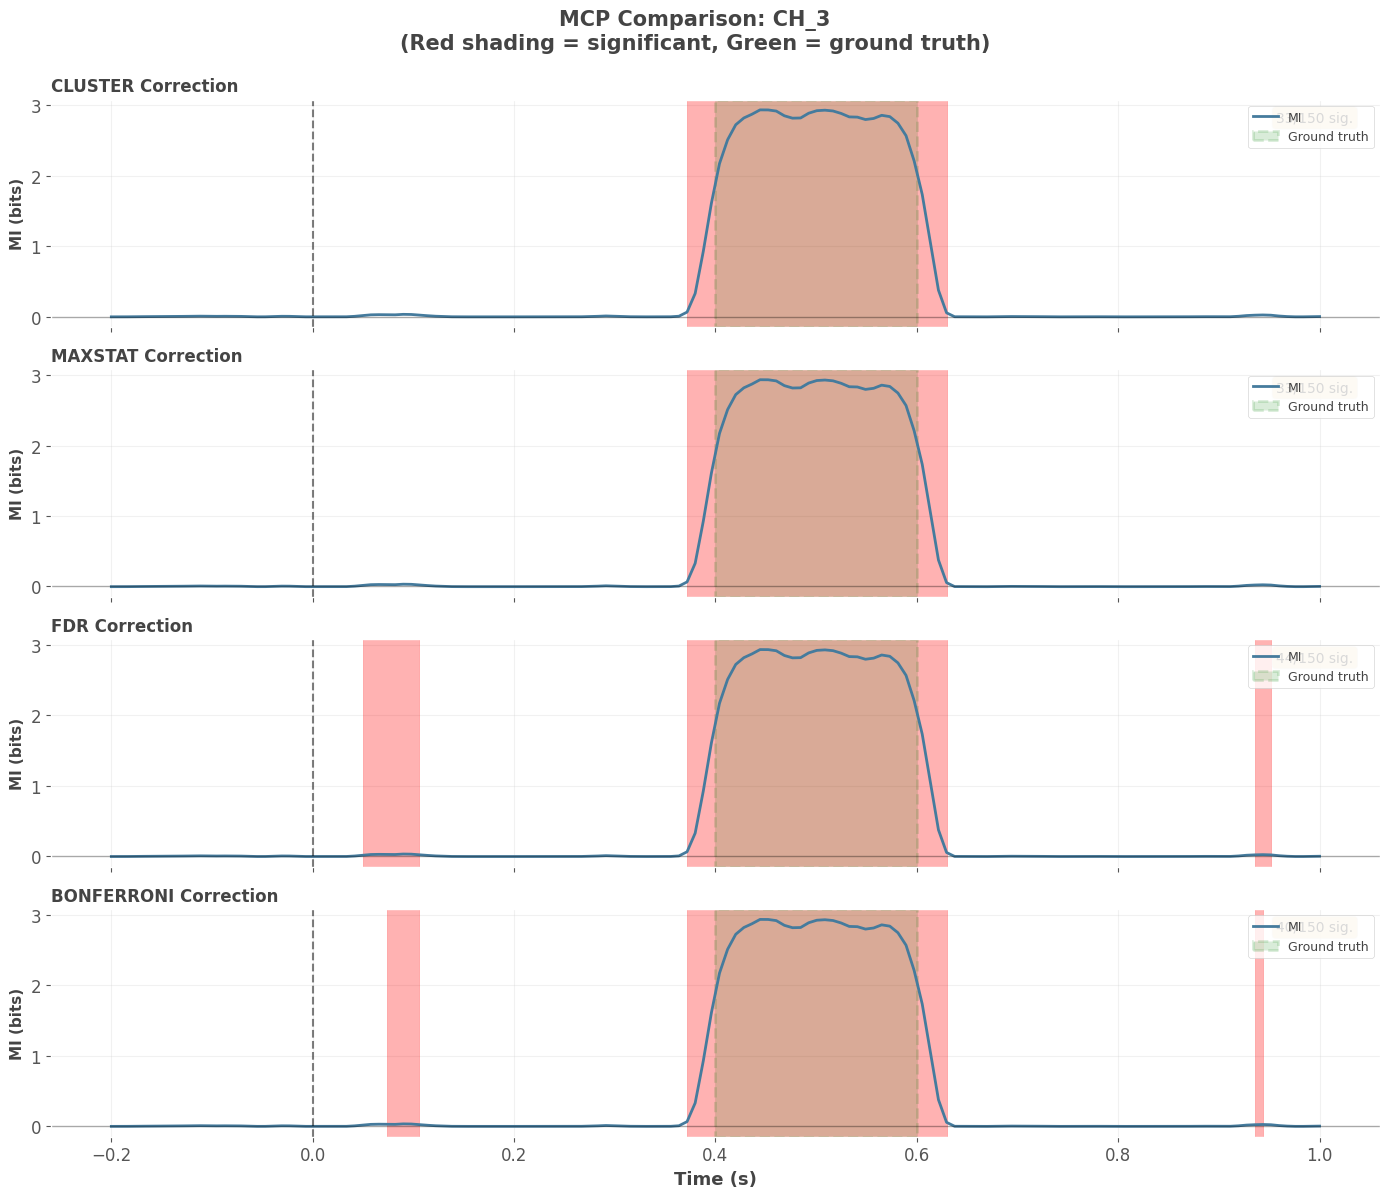
\includegraphics[keepaspectratio]{04_frites_neural_timeseries_files/figure-pdf/cell-9-output-2.png}}

\begin{verbatim}

📊 Comparison Summary:
============================================================
cluster     :  33/150 time points significant
maxstat     :  33/150 time points significant
fdr         :  44/150 time points significant
bonferroni  :  40/150 time points significant

💡 Key Insights:
   • CLUSTER: Best for detecting temporal effects (our case)
   • MAXSTAT: Very conservative, high specificity
   • FDR: More liberal, good for exploration
   • BONFERRONI: Too conservative for time series

🎯 For time-resolved neural data, use 'cluster' correction!
\end{verbatim}

\section{Part 4: Dynamic Functional
Connectivity}\label{part-4-dynamic-functional-connectivity}

\subsection{Beyond Single-Channel
Analysis}\label{beyond-single-channel-analysis}

So far we've looked at how individual brain regions encode task
information. But brains are \textbf{networks} - regions interact and
coordinate. Dynamic Functional Connectivity (DFC) measures how these
interactions change over time.

\textbf{DFC using Mutual Information}:
\[\text{DFC}_{ij}(t) = I(\text{Region}_i(t); \text{Region}_j(t))\]

This quantifies the statistical dependency between two regions at time
\(t\).

\subsection{Why DFC Matters}\label{why-dfc-matters}

\begin{itemize}
\tightlist
\item
  \textbf{Task modulation}: Connectivity increases during task-relevant
  periods
\item
  \textbf{Cognitive states}: Different networks active during attention,
  memory, etc.
\item
  \textbf{Learning}: Connectivity patterns change with experience
\item
  \textbf{Disease}: Altered connectivity in disorders
\end{itemize}

\subsection{Computing DFC with Frites}\label{computing-dfc-with-frites}

Frites provides \texttt{conn\_dfc()} for single-trial dynamic functional
connectivity:

\begin{Shaded}
\begin{Highlighting}[]
\CommentTok{\# We\textquotesingle{}ll compute DFC on sliding windows}
\CommentTok{\# For simplicity, use 3 time windows}

\CommentTok{\# Define windows (in sample indices)}
\NormalTok{win\_samples }\OperatorTok{=}\NormalTok{ np.array([}
\NormalTok{    [}\DecValTok{20}\NormalTok{, }\DecValTok{50}\NormalTok{],   }\CommentTok{\# Early: {-}50ms to 200ms}
\NormalTok{    [}\DecValTok{50}\NormalTok{, }\DecValTok{100}\NormalTok{],  }\CommentTok{\# Middle: 200ms to 650ms (includes task window)}
\NormalTok{    [}\DecValTok{100}\NormalTok{, }\DecValTok{140}\NormalTok{]  }\CommentTok{\# Late: 650ms to 950ms}
\NormalTok{])}

\CommentTok{\# Compute DFC for first subject}
\BuiltInTok{print}\NormalTok{(}\StringTok{"Computing Dynamic Functional Connectivity..."}\NormalTok{)}
\BuiltInTok{print}\NormalTok{(}\SpecialStringTok{f"Windows: }\SpecialCharTok{\{}\BuiltInTok{len}\NormalTok{(win\_samples)}\SpecialCharTok{\}}\SpecialStringTok{"}\NormalTok{)}
\BuiltInTok{print}\NormalTok{(}\SpecialStringTok{f"Data shape: }\SpecialCharTok{\{}\NormalTok{data[}\DecValTok{0}\NormalTok{]}\SpecialCharTok{.}\NormalTok{shape}\SpecialCharTok{\}}\CharTok{\textbackslash{}n}\SpecialStringTok{"}\NormalTok{)}

\NormalTok{dfc }\OperatorTok{=}\NormalTok{ conn\_dfc(}
\NormalTok{    data[}\DecValTok{0}\NormalTok{],              }\CommentTok{\# Single subject data (n\_epochs, n\_channels, n\_times)}
\NormalTok{    win\_sample}\OperatorTok{=}\NormalTok{win\_samples,}
\NormalTok{    times}\OperatorTok{=}\NormalTok{time,}
\NormalTok{    roi}\OperatorTok{=}\NormalTok{rois[}\DecValTok{0}\NormalTok{],}
\NormalTok{    gcrn}\OperatorTok{=}\VariableTok{True}\NormalTok{,            }\CommentTok{\# Gaussian Copula Rank Normalization}
\NormalTok{    n\_jobs}\OperatorTok{=}\DecValTok{1}
\NormalTok{)}

\BuiltInTok{print}\NormalTok{(}\SpecialStringTok{f"DFC shape: }\SpecialCharTok{\{}\NormalTok{dfc}\SpecialCharTok{.}\NormalTok{shape}\SpecialCharTok{\}}\SpecialStringTok{"}\NormalTok{)}
\BuiltInTok{print}\NormalTok{(}\SpecialStringTok{f"  {-} Dimension 0 (}\SpecialCharTok{\{}\NormalTok{dfc}\SpecialCharTok{.}\NormalTok{shape[}\DecValTok{0}\NormalTok{]}\SpecialCharTok{\}}\SpecialStringTok{): Time windows"}\NormalTok{)}
\BuiltInTok{print}\NormalTok{(}\SpecialStringTok{f"  {-} Dimension 1 (}\SpecialCharTok{\{}\NormalTok{dfc}\SpecialCharTok{.}\NormalTok{shape[}\DecValTok{1}\NormalTok{]}\SpecialCharTok{\}}\SpecialStringTok{): ROI pairs"}\NormalTok{)}
\BuiltInTok{print}\NormalTok{(}\SpecialStringTok{f"  {-} Dimension 2 (}\SpecialCharTok{\{}\NormalTok{dfc}\SpecialCharTok{.}\NormalTok{shape[}\DecValTok{2}\NormalTok{]}\SpecialCharTok{\}}\SpecialStringTok{): Trials"}\NormalTok{)}
\BuiltInTok{print}\NormalTok{(}\StringTok{"}\CharTok{\textbackslash{}n}\StringTok{✓ DFC computed for all pairs, all windows, all trials!"}\NormalTok{)}
\end{Highlighting}
\end{Shaded}

\begin{verbatim}
Computing Dynamic Functional Connectivity...
Windows: 3
Data shape: (71, 8, 150)
\end{verbatim}

\begin{verbatim}
DFC shape: (71, 28, 3)
  - Dimension 0 (71): Time windows
  - Dimension 1 (28): ROI pairs
  - Dimension 2 (3): Trials

✓ DFC computed for all pairs, all windows, all trials!
\end{verbatim}

\subsection{Visualizing Dynamic Connectivity
Matrices}\label{visualizing-dynamic-connectivity-matrices}

Let's create connectivity matrices for each time window to see how
network structure evolves:

\begin{Shaded}
\begin{Highlighting}[]
\CommentTok{\# Build connectivity matrices}
\NormalTok{n\_channels }\OperatorTok{=} \BuiltInTok{len}\NormalTok{(rois[}\DecValTok{0}\NormalTok{])}

\NormalTok{fig, axes }\OperatorTok{=}\NormalTok{ plt.subplots(}\DecValTok{1}\NormalTok{, }\DecValTok{3}\NormalTok{, figsize}\OperatorTok{=}\NormalTok{(}\DecValTok{16}\NormalTok{, }\DecValTok{5}\NormalTok{))}

\NormalTok{window\_names }\OperatorTok{=}\NormalTok{ [}\StringTok{\textquotesingle{}Early}\CharTok{\textbackslash{}n}\StringTok{({-}50 to 200ms)\textquotesingle{}}\NormalTok{, }\StringTok{\textquotesingle{}Task}\CharTok{\textbackslash{}n}\StringTok{(200 to 650ms)\textquotesingle{}}\NormalTok{, }\StringTok{\textquotesingle{}Late}\CharTok{\textbackslash{}n}\StringTok{(650 to 950ms)\textquotesingle{}}\NormalTok{]}

\ControlFlowTok{for}\NormalTok{ w\_idx, (ax, win\_name) }\KeywordTok{in} \BuiltInTok{enumerate}\NormalTok{(}\BuiltInTok{zip}\NormalTok{(axes, window\_names)):}
    \CommentTok{\# Initialize connectivity matrix}
\NormalTok{    conn\_matrix }\OperatorTok{=}\NormalTok{ np.zeros((n\_channels, n\_channels))}
    
    \CommentTok{\# Fill in from DFC results}
    \CommentTok{\# DFC returns values for upper triangle of pairs}
\NormalTok{    pair\_idx }\OperatorTok{=} \DecValTok{0}
    \ControlFlowTok{for}\NormalTok{ i }\KeywordTok{in} \BuiltInTok{range}\NormalTok{(n\_channels):}
        \ControlFlowTok{for}\NormalTok{ j }\KeywordTok{in} \BuiltInTok{range}\NormalTok{(i}\OperatorTok{+}\DecValTok{1}\NormalTok{, n\_channels):}
            \CommentTok{\# Average across trials}
\NormalTok{            value }\OperatorTok{=}\NormalTok{ dfc[w\_idx, pair\_idx, :].mean()}
\NormalTok{            conn\_matrix[i, j] }\OperatorTok{=}\NormalTok{ value}
\NormalTok{            conn\_matrix[j, i] }\OperatorTok{=}\NormalTok{ value  }\CommentTok{\# Symmetric}
\NormalTok{            pair\_idx }\OperatorTok{+=} \DecValTok{1}
    
    \CommentTok{\# Plot}
\NormalTok{    im }\OperatorTok{=}\NormalTok{ ax.imshow(conn\_matrix, cmap}\OperatorTok{=}\StringTok{\textquotesingle{}RdYlBu\_r\textquotesingle{}}\NormalTok{, vmin}\OperatorTok{={-}}\FloatTok{0.2}\NormalTok{, vmax}\OperatorTok{=}\FloatTok{0.5}\NormalTok{,}
\NormalTok{                   aspect}\OperatorTok{=}\StringTok{\textquotesingle{}auto\textquotesingle{}}\NormalTok{)}
\NormalTok{    ax.set\_xlabel(}\StringTok{\textquotesingle{}Channel\textquotesingle{}}\NormalTok{, fontsize}\OperatorTok{=}\DecValTok{11}\NormalTok{, fontweight}\OperatorTok{=}\StringTok{\textquotesingle{}bold\textquotesingle{}}\NormalTok{)}
\NormalTok{    ax.set\_ylabel(}\StringTok{\textquotesingle{}Channel\textquotesingle{}}\NormalTok{, fontsize}\OperatorTok{=}\DecValTok{11}\NormalTok{, fontweight}\OperatorTok{=}\StringTok{\textquotesingle{}bold\textquotesingle{}}\NormalTok{)}
\NormalTok{    ax.set\_title(win\_name, fontsize}\OperatorTok{=}\DecValTok{12}\NormalTok{, fontweight}\OperatorTok{=}\StringTok{\textquotesingle{}bold\textquotesingle{}}\NormalTok{)}
    
    \CommentTok{\# Add grid}
\NormalTok{    ax.set\_xticks(}\BuiltInTok{range}\NormalTok{(n\_channels))}
\NormalTok{    ax.set\_yticks(}\BuiltInTok{range}\NormalTok{(n\_channels))}
\NormalTok{    ax.set\_xticklabels([}\SpecialStringTok{f\textquotesingle{}}\SpecialCharTok{\{}\NormalTok{i}\SpecialCharTok{\}}\SpecialStringTok{\textquotesingle{}} \ControlFlowTok{for}\NormalTok{ i }\KeywordTok{in} \BuiltInTok{range}\NormalTok{(n\_channels)], fontsize}\OperatorTok{=}\DecValTok{9}\NormalTok{)}
\NormalTok{    ax.set\_yticklabels([}\SpecialStringTok{f\textquotesingle{}}\SpecialCharTok{\{}\NormalTok{i}\SpecialCharTok{\}}\SpecialStringTok{\textquotesingle{}} \ControlFlowTok{for}\NormalTok{ i }\KeywordTok{in} \BuiltInTok{range}\NormalTok{(n\_channels)], fontsize}\OperatorTok{=}\DecValTok{9}\NormalTok{)}
    
    \CommentTok{\# Highlight task{-}encoding channels}
    \ControlFlowTok{for}\NormalTok{ task\_ch }\KeywordTok{in}\NormalTok{ [}\DecValTok{2}\NormalTok{, }\DecValTok{3}\NormalTok{, }\DecValTok{4}\NormalTok{]:}
\NormalTok{        ax.add\_patch(plt.Rectangle((task\_ch}\OperatorTok{{-}}\FloatTok{0.5}\NormalTok{, }\OperatorTok{{-}}\FloatTok{0.5}\NormalTok{), }\DecValTok{1}\NormalTok{, n\_channels,}
\NormalTok{                                  fill}\OperatorTok{=}\VariableTok{False}\NormalTok{, edgecolor}\OperatorTok{=}\StringTok{\textquotesingle{}green\textquotesingle{}}\NormalTok{, linewidth}\OperatorTok{=}\DecValTok{3}\NormalTok{))}
\NormalTok{        ax.add\_patch(plt.Rectangle((}\OperatorTok{{-}}\FloatTok{0.5}\NormalTok{, task\_ch}\OperatorTok{{-}}\FloatTok{0.5}\NormalTok{), n\_channels, }\DecValTok{1}\NormalTok{,}
\NormalTok{                                  fill}\OperatorTok{=}\VariableTok{False}\NormalTok{, edgecolor}\OperatorTok{=}\StringTok{\textquotesingle{}green\textquotesingle{}}\NormalTok{, linewidth}\OperatorTok{=}\DecValTok{3}\NormalTok{))}
    
    \CommentTok{\# Colorbar}
\NormalTok{    plt.colorbar(im, ax}\OperatorTok{=}\NormalTok{ax, label}\OperatorTok{=}\StringTok{\textquotesingle{}MI (bits)\textquotesingle{}}\NormalTok{, fraction}\OperatorTok{=}\FloatTok{0.046}\NormalTok{, pad}\OperatorTok{=}\FloatTok{0.04}\NormalTok{)}

\NormalTok{plt.suptitle(}\StringTok{\textquotesingle{}Dynamic Functional Connectivity Across Time\textquotesingle{}}\NormalTok{, }
\NormalTok{             fontsize}\OperatorTok{=}\DecValTok{15}\NormalTok{, fontweight}\OperatorTok{=}\StringTok{\textquotesingle{}bold\textquotesingle{}}\NormalTok{, y}\OperatorTok{=}\FloatTok{1.02}\NormalTok{)}
\NormalTok{plt.tight\_layout()}
\NormalTok{plt.show()}

\BuiltInTok{print}\NormalTok{(}\StringTok{"}\CharTok{\textbackslash{}n}\StringTok{💡 Observations:"}\NormalTok{)}
\BuiltInTok{print}\NormalTok{(}\StringTok{"="} \OperatorTok{*} \DecValTok{60}\NormalTok{)}
\BuiltInTok{print}\NormalTok{(}\StringTok{"Green boxes: Task{-}encoding channels (2, 3, 4)"}\NormalTok{)}
\BuiltInTok{print}\NormalTok{(}\StringTok{"}\CharTok{\textbackslash{}n}\StringTok{Look for:"}\NormalTok{)}
\BuiltInTok{print}\NormalTok{(}\StringTok{"  • Increased connectivity in task window (middle panel)"}\NormalTok{)}
\BuiltInTok{print}\NormalTok{(}\StringTok{"  • Connections between task{-}encoding channels"}\NormalTok{)}
\BuiltInTok{print}\NormalTok{(}\StringTok{"  • Time{-}varying patterns"}\NormalTok{)}
\BuiltInTok{print}\NormalTok{(}\StringTok{"}\CharTok{\textbackslash{}n}\StringTok{🎯 DFC reveals the dynamic network structure!"}\NormalTok{)}
\end{Highlighting}
\end{Shaded}

\pandocbounded{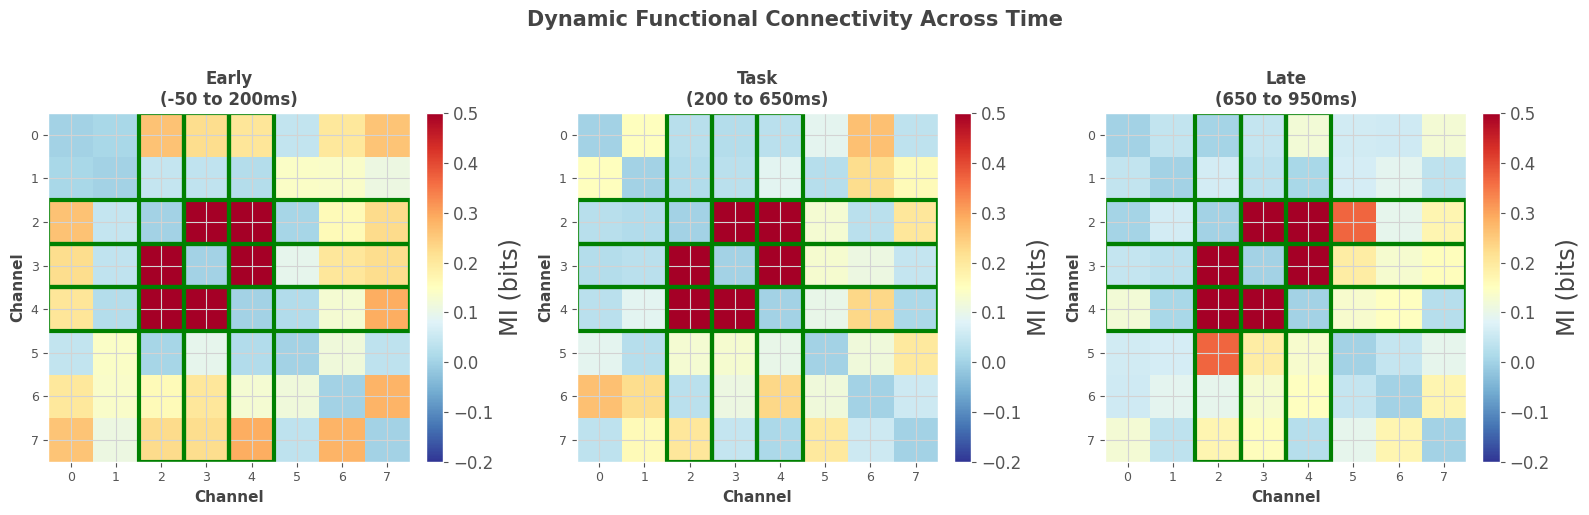
\includegraphics[keepaspectratio]{04_frites_neural_timeseries_files/figure-pdf/cell-11-output-1.png}}

\begin{verbatim}

💡 Observations:
============================================================
Green boxes: Task-encoding channels (2, 3, 4)

Look for:
  • Increased connectivity in task window (middle panel)
  • Connections between task-encoding channels
  • Time-varying patterns

🎯 DFC reveals the dynamic network structure!
\end{verbatim}

\section{Part 5: Multi-Subject Analysis - Fixed vs Random
Effects}\label{part-5-multi-subject-analysis---fixed-vs-random-effects}

\subsection{The Group Analysis
Question}\label{the-group-analysis-question}

In real neuroscience, you typically record from multiple subjects. How
do you combine results to make population-level inferences?

Frites provides two approaches:

\subsection{Fixed-Effect (FFX)
Analysis}\label{fixed-effect-ffx-analysis}

\textbf{What it does}: Pools all trials from all subjects into one big
dataset.

\textbf{Assumption}: The effect is the same across all subjects.

\textbf{Advantages}: - High statistical power (more trials) - Detects
effects that are consistent - Requires fewer subjects

\textbf{Disadvantages}: - Doesn't account for inter-subject variability
- Can't generalize beyond tested subjects - Sensitive to outlier
subjects

\textbf{Use when}: Effect expected to be highly reproducible, or small N
subjects.

\subsection{Random-Effect (RFX)
Analysis}\label{random-effect-rfx-analysis}

\textbf{What it does}: Computes MI per subject, then tests if the effect
is consistent across subjects.

\textbf{Assumption}: The effect varies across subjects from a population
distribution.

\textbf{Advantages}: - Accounts for inter-subject variability\\
- Can generalize to new subjects - Robust to outliers

\textbf{Disadvantages}: - Lower power (fewer effective samples) -
Requires more subjects (typically 15+) - May miss weak but consistent
effects

\textbf{Use when}: Large N subjects, want population inference, expect
variability.

Let's compare both approaches:

\begin{Shaded}
\begin{Highlighting}[]
\CommentTok{\# Create larger multi{-}subject dataset}
\NormalTok{n\_subjects }\OperatorTok{=} \DecValTok{8}  \CommentTok{\# Reasonable for RFX}
\NormalTok{data\_multi, y\_multi, roi\_multi, time\_multi }\OperatorTok{=}\NormalTok{ simulate\_task\_related\_activity(}
\NormalTok{    n\_subjects}\OperatorTok{=}\NormalTok{n\_subjects,}
\NormalTok{    n\_epochs}\OperatorTok{=}\DecValTok{60}\NormalTok{,}
\NormalTok{    n\_channels}\OperatorTok{=}\DecValTok{8}\NormalTok{,}
\NormalTok{    n\_times}\OperatorTok{=}\DecValTok{150}
\NormalTok{)}

\CommentTok{\# Add inter{-}subject variability}
\CommentTok{\# Some subjects have stronger effects}
\ControlFlowTok{for}\NormalTok{ subj }\KeywordTok{in} \BuiltInTok{range}\NormalTok{(n\_subjects):}
    \CommentTok{\# Random strength multiplier (0.5 to 1.5)}
\NormalTok{    strength }\OperatorTok{=} \FloatTok{0.5} \OperatorTok{+}\NormalTok{ np.random.rand() }\OperatorTok{*} \FloatTok{1.0}
    
    \CommentTok{\# Apply to task{-}encoding channels in task window}
\NormalTok{    task\_mask }\OperatorTok{=}\NormalTok{ (time\_multi }\OperatorTok{\textgreater{}=} \FloatTok{0.4}\NormalTok{) }\OperatorTok{\&}\NormalTok{ (time\_multi }\OperatorTok{\textless{}=} \FloatTok{0.6}\NormalTok{)}
    \ControlFlowTok{for}\NormalTok{ ch }\KeywordTok{in}\NormalTok{ [}\DecValTok{2}\NormalTok{, }\DecValTok{3}\NormalTok{, }\DecValTok{4}\NormalTok{]:}
\NormalTok{        data\_multi[subj][:, ch, task\_mask] }\OperatorTok{*=}\NormalTok{ strength}

\NormalTok{ds\_multi }\OperatorTok{=}\NormalTok{ DatasetEphy(x}\OperatorTok{=}\NormalTok{data\_multi, y}\OperatorTok{=}\NormalTok{y\_multi, roi}\OperatorTok{=}\NormalTok{roi\_multi, times}\OperatorTok{=}\NormalTok{time\_multi)}

\BuiltInTok{print}\NormalTok{(}\StringTok{"Multi{-}Subject Dataset Created"}\NormalTok{)}
\BuiltInTok{print}\NormalTok{(}\StringTok{"="} \OperatorTok{*} \DecValTok{60}\NormalTok{)}
\BuiltInTok{print}\NormalTok{(}\SpecialStringTok{f"Subjects: }\SpecialCharTok{\{}\NormalTok{n\_subjects}\SpecialCharTok{\}}\SpecialStringTok{"}\NormalTok{)}
\BuiltInTok{print}\NormalTok{(}\SpecialStringTok{f"Trials per subject: }\SpecialCharTok{\{}\NormalTok{[d.shape[}\DecValTok{0}\NormalTok{] }\ControlFlowTok{for}\NormalTok{ d }\KeywordTok{in}\NormalTok{ data\_multi]}\SpecialCharTok{\}}\SpecialStringTok{"}\NormalTok{)}
\BuiltInTok{print}\NormalTok{(}\SpecialStringTok{f"Total trials: }\SpecialCharTok{\{}\BuiltInTok{sum}\NormalTok{(d.shape[}\DecValTok{0}\NormalTok{] }\ControlFlowTok{for}\NormalTok{ d }\KeywordTok{in}\NormalTok{ data\_multi)}\SpecialCharTok{\}}\SpecialStringTok{"}\NormalTok{)}
\BuiltInTok{print}\NormalTok{(}\StringTok{"}\CharTok{\textbackslash{}n}\StringTok{✨ Inter{-}subject variability included"}\NormalTok{)}
\BuiltInTok{print}\NormalTok{(}\StringTok{"   Effect strength varies across subjects (realistic!)"}\NormalTok{)}
\end{Highlighting}
\end{Shaded}

\begin{verbatim}
Multi-Subject Dataset Created
============================================================
Subjects: 8
Trials per subject: [63, 60, 59, 51, 59, 53, 55, 67]
Total trials: 467

✨ Inter-subject variability included
   Effect strength varies across subjects (realistic!)
\end{verbatim}

\begin{Shaded}
\begin{Highlighting}[]
\CommentTok{\# Compare FFX vs RFX}
\BuiltInTok{print}\NormalTok{(}\StringTok{"}\CharTok{\textbackslash{}n}\StringTok{Comparing Fixed{-}Effect vs Random{-}Effect Analysis"}\NormalTok{)}
\BuiltInTok{print}\NormalTok{(}\StringTok{"="} \OperatorTok{*} \DecValTok{60}\NormalTok{)}

\CommentTok{\# FFX analysis}
\BuiltInTok{print}\NormalTok{(}\StringTok{"}\CharTok{\textbackslash{}n}\StringTok{1. Running FFX (pooled across subjects)..."}\NormalTok{)}
\NormalTok{wf\_ffx }\OperatorTok{=}\NormalTok{ WfMi(mi\_type}\OperatorTok{=}\StringTok{\textquotesingle{}cc\textquotesingle{}}\NormalTok{, inference}\OperatorTok{=}\StringTok{\textquotesingle{}ffx\textquotesingle{}}\NormalTok{, verbose}\OperatorTok{=}\VariableTok{False}\NormalTok{)}
\NormalTok{mi\_ffx, pv\_ffx }\OperatorTok{=}\NormalTok{ wf\_ffx.fit(ds\_multi, n\_perm}\OperatorTok{=}\DecValTok{200}\NormalTok{, mcp}\OperatorTok{=}\StringTok{\textquotesingle{}cluster\textquotesingle{}}\NormalTok{, random\_state}\OperatorTok{=}\DecValTok{42}\NormalTok{)}

\CommentTok{\# RFX analysis  }
\BuiltInTok{print}\NormalTok{(}\StringTok{"2. Running RFX (per{-}subject, then group test)..."}\NormalTok{)}
\NormalTok{wf\_rfx }\OperatorTok{=}\NormalTok{ WfMi(mi\_type}\OperatorTok{=}\StringTok{\textquotesingle{}cc\textquotesingle{}}\NormalTok{, inference}\OperatorTok{=}\StringTok{\textquotesingle{}rfx\textquotesingle{}}\NormalTok{, verbose}\OperatorTok{=}\VariableTok{False}\NormalTok{)}
\NormalTok{mi\_rfx, pv\_rfx }\OperatorTok{=}\NormalTok{ wf\_rfx.fit(ds\_multi, n\_perm}\OperatorTok{=}\DecValTok{200}\NormalTok{, mcp}\OperatorTok{=}\StringTok{\textquotesingle{}cluster\textquotesingle{}}\NormalTok{, random\_state}\OperatorTok{=}\DecValTok{42}\NormalTok{)}

\BuiltInTok{print}\NormalTok{(}\StringTok{"}\CharTok{\textbackslash{}n}\StringTok{Done! Comparing results..."}\NormalTok{)}

\CommentTok{\# Visualize comparison for task{-}encoding channel}
\NormalTok{fig, axes }\OperatorTok{=}\NormalTok{ plt.subplots(}\DecValTok{3}\NormalTok{, }\DecValTok{1}\NormalTok{, figsize}\OperatorTok{=}\NormalTok{(}\DecValTok{14}\NormalTok{, }\DecValTok{12}\NormalTok{), sharex}\OperatorTok{=}\VariableTok{True}\NormalTok{)}

\NormalTok{roi\_name }\OperatorTok{=} \StringTok{\textquotesingle{}CH\_3\textquotesingle{}}

\CommentTok{\# Panel 1: FFX MI}
\NormalTok{ax1 }\OperatorTok{=}\NormalTok{ axes[}\DecValTok{0}\NormalTok{]}
\NormalTok{mi\_ffx\_ch }\OperatorTok{=}\NormalTok{ mi\_ffx.sel(roi}\OperatorTok{=}\NormalTok{roi\_name).squeeze()}
\NormalTok{pv\_ffx\_ch }\OperatorTok{=}\NormalTok{ pv\_ffx.sel(roi}\OperatorTok{=}\NormalTok{roi\_name).squeeze()}
\NormalTok{ax1.plot(time\_multi, mi\_ffx\_ch, linewidth}\OperatorTok{=}\FloatTok{2.5}\NormalTok{, color}\OperatorTok{=}\StringTok{\textquotesingle{}\#E63946\textquotesingle{}}\NormalTok{, label}\OperatorTok{=}\StringTok{\textquotesingle{}FFX MI\textquotesingle{}}\NormalTok{)}
\NormalTok{sig\_ffx }\OperatorTok{=}\NormalTok{ pv\_ffx\_ch.values }\OperatorTok{\textless{}} \FloatTok{0.05}
\ControlFlowTok{if}\NormalTok{ sig\_ffx.}\BuiltInTok{any}\NormalTok{():}
\NormalTok{    ax1.fill\_between(time\_multi, }\DecValTok{0}\NormalTok{, mi\_ffx\_ch, where}\OperatorTok{=}\NormalTok{sig\_ffx, }
\NormalTok{                     alpha}\OperatorTok{=}\FloatTok{0.3}\NormalTok{, color}\OperatorTok{=}\StringTok{\textquotesingle{}red\textquotesingle{}}\NormalTok{, label}\OperatorTok{=}\StringTok{\textquotesingle{}p \textless{} 0.05\textquotesingle{}}\NormalTok{)}
\NormalTok{ax1.axvline(}\DecValTok{0}\NormalTok{, color}\OperatorTok{=}\StringTok{\textquotesingle{}k\textquotesingle{}}\NormalTok{, linestyle}\OperatorTok{=}\StringTok{\textquotesingle{}{-}{-}\textquotesingle{}}\NormalTok{, alpha}\OperatorTok{=}\FloatTok{0.5}\NormalTok{)}
\NormalTok{ax1.axvspan(}\FloatTok{0.4}\NormalTok{, }\FloatTok{0.6}\NormalTok{, alpha}\OperatorTok{=}\FloatTok{0.15}\NormalTok{, color}\OperatorTok{=}\StringTok{\textquotesingle{}green\textquotesingle{}}\NormalTok{, label}\OperatorTok{=}\StringTok{\textquotesingle{}Ground truth\textquotesingle{}}\NormalTok{)}
\NormalTok{ax1.set\_ylabel(}\StringTok{\textquotesingle{}MI (bits)\textquotesingle{}}\NormalTok{, fontsize}\OperatorTok{=}\DecValTok{12}\NormalTok{, fontweight}\OperatorTok{=}\StringTok{\textquotesingle{}bold\textquotesingle{}}\NormalTok{)}
\NormalTok{ax1.set\_title(}\StringTok{\textquotesingle{}Fixed{-}Effect Analysis (FFX)}\CharTok{\textbackslash{}n}\StringTok{Pools all trials from all subjects\textquotesingle{}}\NormalTok{, }
\NormalTok{              fontsize}\OperatorTok{=}\DecValTok{13}\NormalTok{, fontweight}\OperatorTok{=}\StringTok{\textquotesingle{}bold\textquotesingle{}}\NormalTok{)}
\NormalTok{ax1.legend(loc}\OperatorTok{=}\StringTok{\textquotesingle{}upper right\textquotesingle{}}\NormalTok{, fontsize}\OperatorTok{=}\DecValTok{10}\NormalTok{)}
\NormalTok{ax1.grid(}\VariableTok{True}\NormalTok{, alpha}\OperatorTok{=}\FloatTok{0.3}\NormalTok{)}

\CommentTok{\# Panel 2: RFX MI}
\NormalTok{ax2 }\OperatorTok{=}\NormalTok{ axes[}\DecValTok{1}\NormalTok{]}
\NormalTok{mi\_rfx\_ch }\OperatorTok{=}\NormalTok{ mi\_rfx.sel(roi}\OperatorTok{=}\NormalTok{roi\_name).squeeze()}
\NormalTok{pv\_rfx\_ch }\OperatorTok{=}\NormalTok{ pv\_rfx.sel(roi}\OperatorTok{=}\NormalTok{roi\_name).squeeze()}
\NormalTok{ax2.plot(time\_multi, mi\_rfx\_ch, linewidth}\OperatorTok{=}\FloatTok{2.5}\NormalTok{, color}\OperatorTok{=}\StringTok{\textquotesingle{}\#457B9D\textquotesingle{}}\NormalTok{, label}\OperatorTok{=}\StringTok{\textquotesingle{}RFX MI\textquotesingle{}}\NormalTok{)}
\NormalTok{sig\_rfx }\OperatorTok{=}\NormalTok{ pv\_rfx\_ch.values }\OperatorTok{\textless{}} \FloatTok{0.05}
\ControlFlowTok{if}\NormalTok{ sig\_rfx.}\BuiltInTok{any}\NormalTok{():}
\NormalTok{    ax2.fill\_between(time\_multi, }\DecValTok{0}\NormalTok{, mi\_rfx\_ch, where}\OperatorTok{=}\NormalTok{sig\_rfx,}
\NormalTok{                     alpha}\OperatorTok{=}\FloatTok{0.3}\NormalTok{, color}\OperatorTok{=}\StringTok{\textquotesingle{}blue\textquotesingle{}}\NormalTok{, label}\OperatorTok{=}\StringTok{\textquotesingle{}p \textless{} 0.05\textquotesingle{}}\NormalTok{)}
\NormalTok{ax2.axvline(}\DecValTok{0}\NormalTok{, color}\OperatorTok{=}\StringTok{\textquotesingle{}k\textquotesingle{}}\NormalTok{, linestyle}\OperatorTok{=}\StringTok{\textquotesingle{}{-}{-}\textquotesingle{}}\NormalTok{, alpha}\OperatorTok{=}\FloatTok{0.5}\NormalTok{)}
\NormalTok{ax2.axvspan(}\FloatTok{0.4}\NormalTok{, }\FloatTok{0.6}\NormalTok{, alpha}\OperatorTok{=}\FloatTok{0.15}\NormalTok{, color}\OperatorTok{=}\StringTok{\textquotesingle{}green\textquotesingle{}}\NormalTok{, label}\OperatorTok{=}\StringTok{\textquotesingle{}Ground truth\textquotesingle{}}\NormalTok{)}
\NormalTok{ax2.set\_ylabel(}\StringTok{\textquotesingle{}MI (bits)\textquotesingle{}}\NormalTok{, fontsize}\OperatorTok{=}\DecValTok{12}\NormalTok{, fontweight}\OperatorTok{=}\StringTok{\textquotesingle{}bold\textquotesingle{}}\NormalTok{)}
\NormalTok{ax2.set\_title(}\StringTok{\textquotesingle{}Random{-}Effect Analysis (RFX)}\CharTok{\textbackslash{}n}\StringTok{Models inter{-}subject variability\textquotesingle{}}\NormalTok{, }
\NormalTok{              fontsize}\OperatorTok{=}\DecValTok{13}\NormalTok{, fontweight}\OperatorTok{=}\StringTok{\textquotesingle{}bold\textquotesingle{}}\NormalTok{)}
\NormalTok{ax2.legend(loc}\OperatorTok{=}\StringTok{\textquotesingle{}upper right\textquotesingle{}}\NormalTok{, fontsize}\OperatorTok{=}\DecValTok{10}\NormalTok{)}
\NormalTok{ax2.grid(}\VariableTok{True}\NormalTok{, alpha}\OperatorTok{=}\FloatTok{0.3}\NormalTok{)}

\CommentTok{\# Panel 3: Direct comparison}
\NormalTok{ax3 }\OperatorTok{=}\NormalTok{ axes[}\DecValTok{2}\NormalTok{]}
\NormalTok{ax3.plot(time\_multi, mi\_ffx\_ch, linewidth}\OperatorTok{=}\FloatTok{2.5}\NormalTok{, color}\OperatorTok{=}\StringTok{\textquotesingle{}\#E63946\textquotesingle{}}\NormalTok{, }
\NormalTok{         label}\OperatorTok{=}\StringTok{\textquotesingle{}FFX\textquotesingle{}}\NormalTok{, alpha}\OperatorTok{=}\FloatTok{0.8}\NormalTok{)}
\NormalTok{ax3.plot(time\_multi, mi\_rfx\_ch, linewidth}\OperatorTok{=}\FloatTok{2.5}\NormalTok{, color}\OperatorTok{=}\StringTok{\textquotesingle{}\#457B9D\textquotesingle{}}\NormalTok{, }
\NormalTok{         label}\OperatorTok{=}\StringTok{\textquotesingle{}RFX\textquotesingle{}}\NormalTok{, alpha}\OperatorTok{=}\FloatTok{0.8}\NormalTok{)}
\NormalTok{ax3.axvline(}\DecValTok{0}\NormalTok{, color}\OperatorTok{=}\StringTok{\textquotesingle{}k\textquotesingle{}}\NormalTok{, linestyle}\OperatorTok{=}\StringTok{\textquotesingle{}{-}{-}\textquotesingle{}}\NormalTok{, alpha}\OperatorTok{=}\FloatTok{0.5}\NormalTok{)}
\NormalTok{ax3.axvspan(}\FloatTok{0.4}\NormalTok{, }\FloatTok{0.6}\NormalTok{, alpha}\OperatorTok{=}\FloatTok{0.15}\NormalTok{, color}\OperatorTok{=}\StringTok{\textquotesingle{}green\textquotesingle{}}\NormalTok{)}
\NormalTok{ax3.set\_xlabel(}\StringTok{\textquotesingle{}Time (s)\textquotesingle{}}\NormalTok{, fontsize}\OperatorTok{=}\DecValTok{13}\NormalTok{, fontweight}\OperatorTok{=}\StringTok{\textquotesingle{}bold\textquotesingle{}}\NormalTok{)}
\NormalTok{ax3.set\_ylabel(}\StringTok{\textquotesingle{}MI (bits)\textquotesingle{}}\NormalTok{, fontsize}\OperatorTok{=}\DecValTok{12}\NormalTok{, fontweight}\OperatorTok{=}\StringTok{\textquotesingle{}bold\textquotesingle{}}\NormalTok{)}
\NormalTok{ax3.set\_title(}\StringTok{\textquotesingle{}FFX vs RFX Comparison\textquotesingle{}}\NormalTok{, fontsize}\OperatorTok{=}\DecValTok{13}\NormalTok{, fontweight}\OperatorTok{=}\StringTok{\textquotesingle{}bold\textquotesingle{}}\NormalTok{)}
\NormalTok{ax3.legend(fontsize}\OperatorTok{=}\DecValTok{11}\NormalTok{, loc}\OperatorTok{=}\StringTok{\textquotesingle{}upper right\textquotesingle{}}\NormalTok{)}
\NormalTok{ax3.grid(}\VariableTok{True}\NormalTok{, alpha}\OperatorTok{=}\FloatTok{0.3}\NormalTok{)}

\CommentTok{\# Add difference annotation}
\NormalTok{max\_diff }\OperatorTok{=}\NormalTok{ np.}\BuiltInTok{abs}\NormalTok{(mi\_ffx\_ch.values }\OperatorTok{{-}}\NormalTok{ mi\_rfx\_ch.values).}\BuiltInTok{max}\NormalTok{()}
\NormalTok{ax3.text(}\FloatTok{0.02}\NormalTok{, }\FloatTok{0.95}\NormalTok{, }\SpecialStringTok{f\textquotesingle{}Max difference: }\SpecialCharTok{\{}\NormalTok{max\_diff}\SpecialCharTok{:.4f\}}\SpecialStringTok{ bits\textquotesingle{}}\NormalTok{, }
\NormalTok{         transform}\OperatorTok{=}\NormalTok{ax3.transAxes, fontsize}\OperatorTok{=}\DecValTok{10}\NormalTok{,}
\NormalTok{         bbox}\OperatorTok{=}\BuiltInTok{dict}\NormalTok{(boxstyle}\OperatorTok{=}\StringTok{\textquotesingle{}round\textquotesingle{}}\NormalTok{, facecolor}\OperatorTok{=}\StringTok{\textquotesingle{}wheat\textquotesingle{}}\NormalTok{, alpha}\OperatorTok{=}\FloatTok{0.8}\NormalTok{),}
\NormalTok{         verticalalignment}\OperatorTok{=}\StringTok{\textquotesingle{}top\textquotesingle{}}\NormalTok{)}

\NormalTok{plt.tight\_layout()}
\NormalTok{plt.show()}

\CommentTok{\# Compare detection sensitivity}
\BuiltInTok{print}\NormalTok{(}\StringTok{"}\CharTok{\textbackslash{}n}\StringTok{📊 Detection Comparison:"}\NormalTok{)}
\BuiltInTok{print}\NormalTok{(}\StringTok{"="} \OperatorTok{*} \DecValTok{60}\NormalTok{)}
\NormalTok{n\_sig\_ffx }\OperatorTok{=}\NormalTok{ sig\_ffx.}\BuiltInTok{sum}\NormalTok{()}
\NormalTok{n\_sig\_rfx }\OperatorTok{=}\NormalTok{ sig\_rfx.}\BuiltInTok{sum}\NormalTok{()}
\BuiltInTok{print}\NormalTok{(}\SpecialStringTok{f"FFX: }\SpecialCharTok{\{}\NormalTok{n\_sig\_ffx}\SpecialCharTok{\}}\SpecialStringTok{/}\SpecialCharTok{\{}\BuiltInTok{len}\NormalTok{(time\_multi)}\SpecialCharTok{\}}\SpecialStringTok{ time points significant"}\NormalTok{)}
\BuiltInTok{print}\NormalTok{(}\SpecialStringTok{f"RFX: }\SpecialCharTok{\{}\NormalTok{n\_sig\_rfx}\SpecialCharTok{\}}\SpecialStringTok{/}\SpecialCharTok{\{}\BuiltInTok{len}\NormalTok{(time\_multi)}\SpecialCharTok{\}}\SpecialStringTok{ time points significant"}\NormalTok{)}

\ControlFlowTok{if}\NormalTok{ n\_sig\_ffx }\OperatorTok{\textgreater{}}\NormalTok{ n\_sig\_rfx:}
    \BuiltInTok{print}\NormalTok{(}\StringTok{"}\CharTok{\textbackslash{}n}\StringTok{→ FFX detected more (higher power from pooling)"}\NormalTok{)}
\ControlFlowTok{elif}\NormalTok{ n\_sig\_rfx }\OperatorTok{\textgreater{}}\NormalTok{ n\_sig\_ffx:}
    \BuiltInTok{print}\NormalTok{(}\StringTok{"}\CharTok{\textbackslash{}n}\StringTok{→ RFX detected more (accounting for variability helped)"}\NormalTok{)}
\ControlFlowTok{else}\NormalTok{:}
    \BuiltInTok{print}\NormalTok{(}\StringTok{"}\CharTok{\textbackslash{}n}\StringTok{→ Both detected same regions"}\NormalTok{)}

\BuiltInTok{print}\NormalTok{(}\StringTok{"}\CharTok{\textbackslash{}n}\StringTok{💡 Practical Guidance:"}\NormalTok{)}
\BuiltInTok{print}\NormalTok{(}\StringTok{"   • Small N subjects (\textless{}10): Use FFX"}\NormalTok{)}
\BuiltInTok{print}\NormalTok{(}\StringTok{"   • Large N subjects (15+): Use RFX for generalization"}\NormalTok{)}
\BuiltInTok{print}\NormalTok{(}\StringTok{"   • High variability expected: Use RFX"}\NormalTok{)}
\BuiltInTok{print}\NormalTok{(}\StringTok{"   • Exploratory analysis: Try both, see if consistent"}\NormalTok{)}
\end{Highlighting}
\end{Shaded}

\begin{verbatim}

Comparing Fixed-Effect vs Random-Effect Analysis
============================================================

1. Running FFX (pooled across subjects)...
2. Running RFX (per-subject, then group test)...

Done! Comparing results...
\end{verbatim}

\pandocbounded{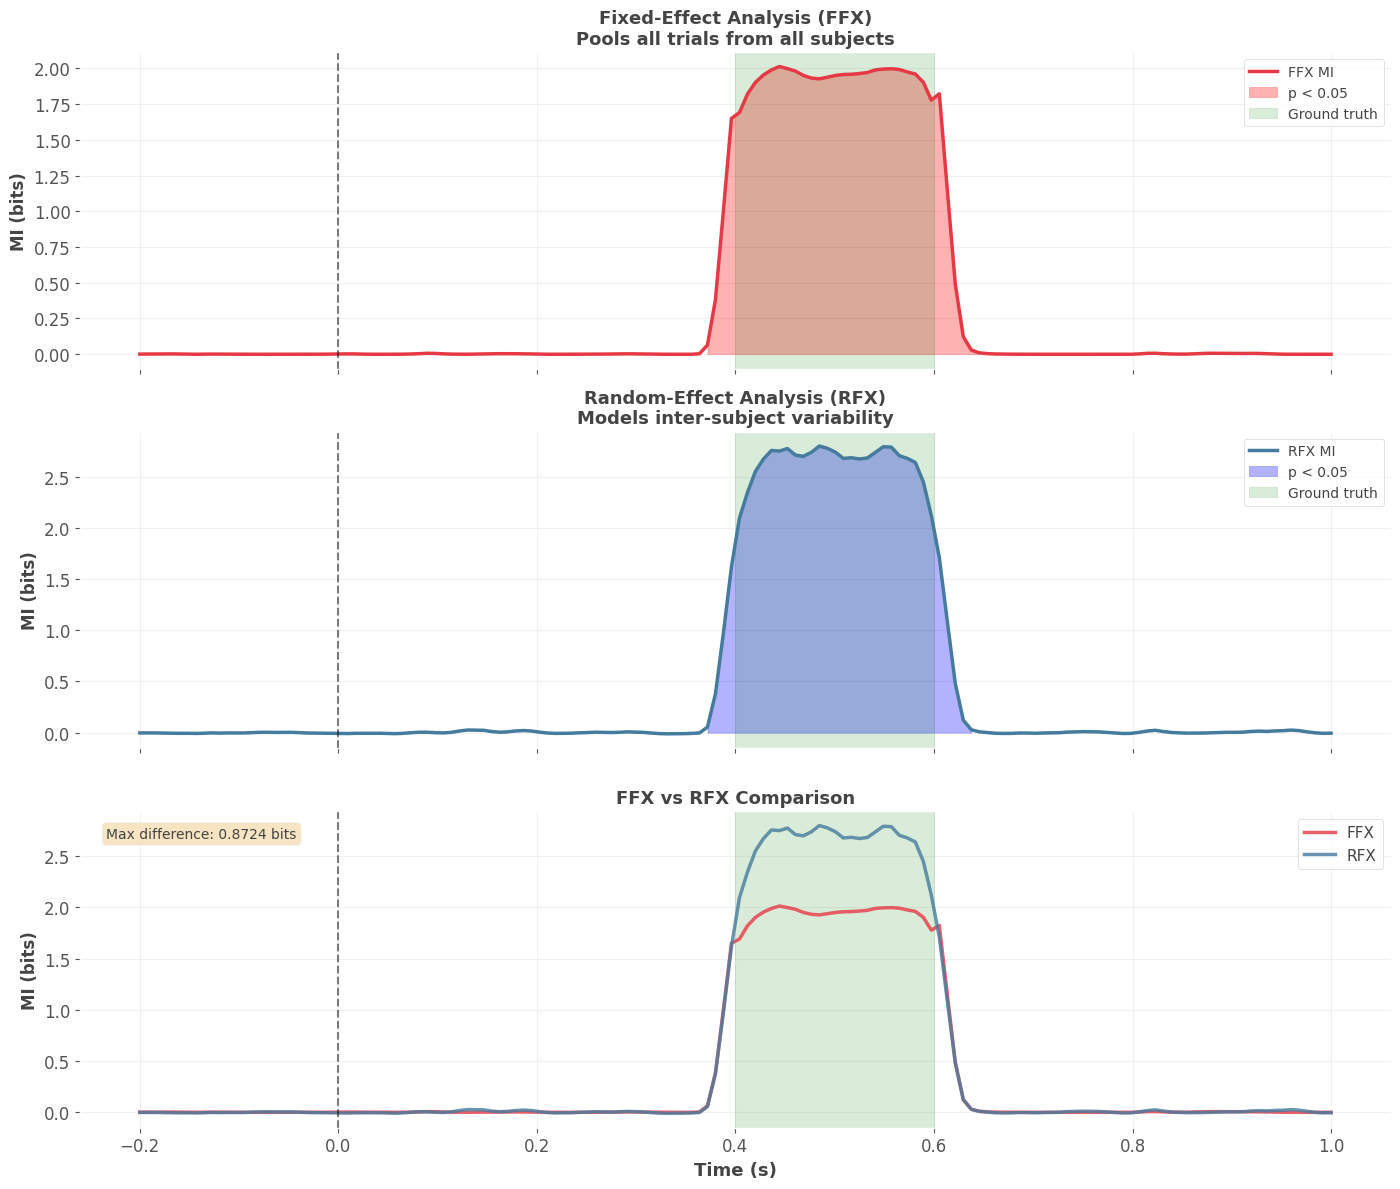
\includegraphics[keepaspectratio]{04_frites_neural_timeseries_files/figure-pdf/cell-13-output-2.png}}

\begin{verbatim}

📊 Detection Comparison:
============================================================
FFX: 35/150 time points significant
RFX: 34/150 time points significant

→ FFX detected more (higher power from pooling)

💡 Practical Guidance:
   • Small N subjects (<10): Use FFX
   • Large N subjects (15+): Use RFX for generalization
   • High variability expected: Use RFX
   • Exploratory analysis: Try both, see if consistent
\end{verbatim}

\section{Part 6: Realistic Application - Visual Attention
Experiment}\label{part-6-realistic-application---visual-attention-experiment}

\subsection{Experimental Paradigm}\label{experimental-paradigm}

Let's simulate a realistic attention experiment:

\textbf{Task}: Subjects view oriented gratings and must report whether
they're tilted left or right.

\textbf{Conditions}: - \textbf{Attended}: Grating is at attended
location - \textbf{Unattended}: Grating is at unattended location

\textbf{Hypothesis}: Neural information about orientation should be
higher in attended condition.

\textbf{Prediction}: MI between neural activity and orientation should:
- Emerge around 100-200ms (early visual processing) - Be stronger in
attended condition - Show different patterns in V1 vs higher areas

Let's simulate this experiment and analyze with Frites:

\begin{Shaded}
\begin{Highlighting}[]
\KeywordTok{def}\NormalTok{ simulate\_attention\_experiment(n\_subjects}\OperatorTok{=}\DecValTok{6}\NormalTok{, n\_trials\_per\_cond}\OperatorTok{=}\DecValTok{60}\NormalTok{):}
    \CommentTok{"""}
\CommentTok{    Simulate attention modulation of orientation coding.}
\CommentTok{    """}
\NormalTok{    n\_channels }\OperatorTok{=} \DecValTok{6}  \CommentTok{\# V1, V2, V4 (2 channels each)}
\NormalTok{    n\_times }\OperatorTok{=} \DecValTok{200}
\NormalTok{    time }\OperatorTok{=}\NormalTok{ np.linspace(}\OperatorTok{{-}}\FloatTok{0.2}\NormalTok{, }\FloatTok{0.8}\NormalTok{, n\_times)}
    
\NormalTok{    data\_list }\OperatorTok{=}\NormalTok{ []}
\NormalTok{    orientation\_list }\OperatorTok{=}\NormalTok{ []}
\NormalTok{    attention\_list }\OperatorTok{=}\NormalTok{ []}
\NormalTok{    roi\_list }\OperatorTok{=}\NormalTok{ []}
    
    \ControlFlowTok{for}\NormalTok{ subj }\KeywordTok{in} \BuiltInTok{range}\NormalTok{(n\_subjects):}
        \CommentTok{\# Total trials (attended + unattended)}
\NormalTok{        n\_total }\OperatorTok{=}\NormalTok{ n\_trials\_per\_cond }\OperatorTok{*} \DecValTok{2}
        
        \CommentTok{\# Generate orientations (continuous, 0{-}180 degrees)}
\NormalTok{        orientations }\OperatorTok{=}\NormalTok{ np.random.rand(n\_total) }\OperatorTok{*} \DecValTok{180}
        
        \CommentTok{\# Attention condition (0=unattended, 1=attended)}
\NormalTok{        attention }\OperatorTok{=}\NormalTok{ np.concatenate([np.zeros(n\_trials\_per\_cond), }
\NormalTok{                                   np.ones(n\_trials\_per\_cond)]).astype(}\BuiltInTok{int}\NormalTok{)}
        \CommentTok{\# Shuffle}
\NormalTok{        shuffle\_idx }\OperatorTok{=}\NormalTok{ np.random.permutation(n\_total)}
\NormalTok{        orientations }\OperatorTok{=}\NormalTok{ orientations[shuffle\_idx]}
\NormalTok{        attention }\OperatorTok{=}\NormalTok{ attention[shuffle\_idx]}
        
        \CommentTok{\# Initialize neural data}
\NormalTok{        subj\_data }\OperatorTok{=}\NormalTok{ np.random.randn(n\_total, n\_channels, n\_times) }\OperatorTok{*} \FloatTok{0.8}
        
        \CommentTok{\# Add orientation tuning to V1 channels (0, 1)}
        \CommentTok{\# Tuning emerges at 100{-}400ms}
\NormalTok{        tuning\_window }\OperatorTok{=}\NormalTok{ (time }\OperatorTok{\textgreater{}=} \FloatTok{0.1}\NormalTok{) }\OperatorTok{\&}\NormalTok{ (time }\OperatorTok{\textless{}=} \FloatTok{0.4}\NormalTok{)}
        \ControlFlowTok{for}\NormalTok{ trial }\KeywordTok{in} \BuiltInTok{range}\NormalTok{(n\_total):}
\NormalTok{            ori }\OperatorTok{=}\NormalTok{ orientations[trial]}
\NormalTok{            attn }\OperatorTok{=}\NormalTok{ attention[trial]}
            
            \CommentTok{\# V1 channels: weak tuning, minimal attention effect}
            \ControlFlowTok{for}\NormalTok{ v1\_ch }\KeywordTok{in}\NormalTok{ [}\DecValTok{0}\NormalTok{, }\DecValTok{1}\NormalTok{]:}
\NormalTok{                pref\_ori }\OperatorTok{=}\NormalTok{ v1\_ch }\OperatorTok{*} \DecValTok{90}  \CommentTok{\# 0° and 90° preferences}
\NormalTok{                tuning }\OperatorTok{=}\NormalTok{ np.cos(np.deg2rad(ori }\OperatorTok{{-}}\NormalTok{ pref\_ori))}
\NormalTok{                strength }\OperatorTok{=} \FloatTok{1.0} \OperatorTok{+}\NormalTok{ attn }\OperatorTok{*} \FloatTok{0.3}  \CommentTok{\# 30\% boost with attention}
\NormalTok{                subj\_data[trial, v1\_ch, tuning\_window] }\OperatorTok{+=}\NormalTok{ tuning }\OperatorTok{*}\NormalTok{ strength }\OperatorTok{*} \FloatTok{0.8}
            
            \CommentTok{\# V4 channels: strong tuning, strong attention effect}
            \ControlFlowTok{for}\NormalTok{ v4\_ch }\KeywordTok{in}\NormalTok{ [}\DecValTok{4}\NormalTok{, }\DecValTok{5}\NormalTok{]:}
\NormalTok{                pref\_ori }\OperatorTok{=}\NormalTok{ (v4\_ch }\OperatorTok{{-}} \DecValTok{4}\NormalTok{) }\OperatorTok{*} \DecValTok{90}
\NormalTok{                tuning }\OperatorTok{=}\NormalTok{ np.cos(np.deg2rad(ori }\OperatorTok{{-}}\NormalTok{ pref\_ori))}
\NormalTok{                strength }\OperatorTok{=} \FloatTok{1.0} \OperatorTok{+}\NormalTok{ attn }\OperatorTok{*} \FloatTok{1.2}  \CommentTok{\# 120\% boost with attention!}
\NormalTok{                subj\_data[trial, v4\_ch, tuning\_window] }\OperatorTok{+=}\NormalTok{ tuning }\OperatorTok{*}\NormalTok{ strength }\OperatorTok{*} \FloatTok{1.5}
        
        \CommentTok{\# Smooth temporally}
        \ImportTok{from}\NormalTok{ scipy.ndimage }\ImportTok{import}\NormalTok{ gaussian\_filter1d}
        \ControlFlowTok{for}\NormalTok{ ep }\KeywordTok{in} \BuiltInTok{range}\NormalTok{(n\_total):}
            \ControlFlowTok{for}\NormalTok{ ch }\KeywordTok{in} \BuiltInTok{range}\NormalTok{(n\_channels):}
\NormalTok{                subj\_data[ep, ch, :] }\OperatorTok{=}\NormalTok{ gaussian\_filter1d(subj\_data[ep, ch, :], sigma}\OperatorTok{=}\DecValTok{3}\NormalTok{)}
        
\NormalTok{        data\_list.append(subj\_data)}
\NormalTok{        orientation\_list.append(orientations)}
\NormalTok{        attention\_list.append(attention)}
\NormalTok{        roi\_list.append([}\StringTok{\textquotesingle{}V1\_L\textquotesingle{}}\NormalTok{, }\StringTok{\textquotesingle{}V1\_R\textquotesingle{}}\NormalTok{, }\StringTok{\textquotesingle{}V2\_L\textquotesingle{}}\NormalTok{, }\StringTok{\textquotesingle{}V2\_R\textquotesingle{}}\NormalTok{, }\StringTok{\textquotesingle{}V4\_L\textquotesingle{}}\NormalTok{, }\StringTok{\textquotesingle{}V4\_R\textquotesingle{}}\NormalTok{])}
    
    \ControlFlowTok{return}\NormalTok{ data\_list, orientation\_list, attention\_list, roi\_list, time}

\CommentTok{\# Generate attention experiment data}
\NormalTok{data\_attn, oris\_attn, attn\_attn, rois\_attn, time\_attn }\OperatorTok{=}\NormalTok{ simulate\_attention\_experiment()}

\BuiltInTok{print}\NormalTok{(}\StringTok{"Attention Experiment Simulated"}\NormalTok{)}
\BuiltInTok{print}\NormalTok{(}\StringTok{"="} \OperatorTok{*} \DecValTok{60}\NormalTok{)}
\BuiltInTok{print}\NormalTok{(}\SpecialStringTok{f"Subjects: }\SpecialCharTok{\{}\BuiltInTok{len}\NormalTok{(data\_attn)}\SpecialCharTok{\}}\SpecialStringTok{"}\NormalTok{)}
\BuiltInTok{print}\NormalTok{(}\SpecialStringTok{f"ROIs: }\SpecialCharTok{\{}\NormalTok{rois\_attn[}\DecValTok{0}\NormalTok{]}\SpecialCharTok{\}}\SpecialStringTok{"}\NormalTok{)}
\BuiltInTok{print}\NormalTok{(}\SpecialStringTok{f"}\CharTok{\textbackslash{}n}\SpecialStringTok{Task design:"}\NormalTok{)}
\BuiltInTok{print}\NormalTok{(}\SpecialStringTok{f"  {-} Continuous orientation: 0{-}180°"}\NormalTok{)}
\BuiltInTok{print}\NormalTok{(}\SpecialStringTok{f"  {-} Binary attention: attended vs unattended"}\NormalTok{)}
\BuiltInTok{print}\NormalTok{(}\SpecialStringTok{f"  {-} V1: Weak tuning, minimal attention effect"}\NormalTok{)}
\BuiltInTok{print}\NormalTok{(}\SpecialStringTok{f"  {-} V4: Strong tuning, strong attention effect"}\NormalTok{)}
\BuiltInTok{print}\NormalTok{(}\StringTok{"}\CharTok{\textbackslash{}n}\StringTok{🎯 Research Question: Does attention modulate orientation information?"}\NormalTok{)}
\end{Highlighting}
\end{Shaded}

\begin{verbatim}
Attention Experiment Simulated
============================================================
Subjects: 6
ROIs: ['V1_L', 'V1_R', 'V2_L', 'V2_R', 'V4_L', 'V4_R']

Task design:
  - Continuous orientation: 0-180°
  - Binary attention: attended vs unattended
  - V1: Weak tuning, minimal attention effect
  - V4: Strong tuning, strong attention effect

🎯 Research Question: Does attention modulate orientation information?
\end{verbatim}

\subsection{Analysis 1: Overall Orientation
Information}\label{analysis-1-overall-orientation-information}

First, let's compute MI between neural activity and orientation
(ignoring attention for now):

\begin{Shaded}
\begin{Highlighting}[]
\CommentTok{\# Create dataset with orientation as task variable}
\NormalTok{ds\_ori }\OperatorTok{=}\NormalTok{ DatasetEphy(x}\OperatorTok{=}\NormalTok{data\_attn, y}\OperatorTok{=}\NormalTok{oris\_attn, roi}\OperatorTok{=}\NormalTok{rois\_attn, times}\OperatorTok{=}\NormalTok{time\_attn)}

\BuiltInTok{print}\NormalTok{(}\StringTok{"Computing I(Neural; Orientation) across time..."}\NormalTok{)}

\CommentTok{\# Workflow for continuous orientation}
\NormalTok{wf\_ori }\OperatorTok{=}\NormalTok{ WfMi(mi\_type}\OperatorTok{=}\StringTok{\textquotesingle{}cc\textquotesingle{}}\NormalTok{, inference}\OperatorTok{=}\StringTok{\textquotesingle{}rfx\textquotesingle{}}\NormalTok{, verbose}\OperatorTok{=}\VariableTok{False}\NormalTok{)}
\NormalTok{mi\_ori, pv\_ori }\OperatorTok{=}\NormalTok{ wf\_ori.fit(ds\_ori, n\_perm}\OperatorTok{=}\DecValTok{200}\NormalTok{, mcp}\OperatorTok{=}\StringTok{\textquotesingle{}cluster\textquotesingle{}}\NormalTok{, random\_state}\OperatorTok{=}\DecValTok{42}\NormalTok{)}

\BuiltInTok{print}\NormalTok{(}\StringTok{"Done!}\CharTok{\textbackslash{}n}\StringTok{"}\NormalTok{)}

\CommentTok{\# Plot results for all ROIs}
\NormalTok{fig, axes }\OperatorTok{=}\NormalTok{ plt.subplots(}\DecValTok{3}\NormalTok{, }\DecValTok{2}\NormalTok{, figsize}\OperatorTok{=}\NormalTok{(}\DecValTok{15}\NormalTok{, }\DecValTok{12}\NormalTok{))}
\NormalTok{axes }\OperatorTok{=}\NormalTok{ axes.flatten()}

\ControlFlowTok{for}\NormalTok{ idx, roi\_name }\KeywordTok{in} \BuiltInTok{enumerate}\NormalTok{(rois\_attn[}\DecValTok{0}\NormalTok{]):}
\NormalTok{    ax }\OperatorTok{=}\NormalTok{ axes[idx]}
    
\NormalTok{    mi\_roi }\OperatorTok{=}\NormalTok{ mi\_ori.sel(roi}\OperatorTok{=}\NormalTok{roi\_name).squeeze()}
\NormalTok{    pv\_roi }\OperatorTok{=}\NormalTok{ pv\_ori.sel(roi}\OperatorTok{=}\NormalTok{roi\_name).squeeze()}
    
    \CommentTok{\# Determine color by area}
    \ControlFlowTok{if} \StringTok{\textquotesingle{}V1\textquotesingle{}} \KeywordTok{in}\NormalTok{ roi\_name:}
\NormalTok{        color }\OperatorTok{=} \StringTok{\textquotesingle{}\#E63946\textquotesingle{}}
    \ControlFlowTok{elif} \StringTok{\textquotesingle{}V2\textquotesingle{}} \KeywordTok{in}\NormalTok{ roi\_name:}
\NormalTok{        color }\OperatorTok{=} \StringTok{\textquotesingle{}\#F1FAEE\textquotesingle{}}
    \ControlFlowTok{else}\NormalTok{:  }\CommentTok{\# V4}
\NormalTok{        color }\OperatorTok{=} \StringTok{\textquotesingle{}\#457B9D\textquotesingle{}}
    
    \CommentTok{\# Plot MI}
\NormalTok{    ax.plot(time\_attn, mi\_roi, linewidth}\OperatorTok{=}\FloatTok{2.5}\NormalTok{, color}\OperatorTok{=}\NormalTok{color, label}\OperatorTok{=}\StringTok{\textquotesingle{}MI\textquotesingle{}}\NormalTok{)}
    
    \CommentTok{\# Shade significant regions}
\NormalTok{    sig }\OperatorTok{=}\NormalTok{ pv\_roi.values }\OperatorTok{\textless{}} \FloatTok{0.05}
    \ControlFlowTok{if}\NormalTok{ sig.}\BuiltInTok{any}\NormalTok{():}
\NormalTok{        ax.fill\_between(time\_attn, }\DecValTok{0}\NormalTok{, mi\_roi, where}\OperatorTok{=}\NormalTok{sig, alpha}\OperatorTok{=}\FloatTok{0.3}\NormalTok{, color}\OperatorTok{=}\NormalTok{color)}
    
    \CommentTok{\# Reference lines}
\NormalTok{    ax.axvline(}\DecValTok{0}\NormalTok{, color}\OperatorTok{=}\StringTok{\textquotesingle{}k\textquotesingle{}}\NormalTok{, linestyle}\OperatorTok{=}\StringTok{\textquotesingle{}{-}{-}\textquotesingle{}}\NormalTok{, alpha}\OperatorTok{=}\FloatTok{0.5}\NormalTok{, label}\OperatorTok{=}\StringTok{\textquotesingle{}Stimulus\textquotesingle{}}\NormalTok{)}
\NormalTok{    ax.axhline(}\DecValTok{0}\NormalTok{, color}\OperatorTok{=}\StringTok{\textquotesingle{}k\textquotesingle{}}\NormalTok{, linestyle}\OperatorTok{=}\StringTok{\textquotesingle{}{-}\textquotesingle{}}\NormalTok{, alpha}\OperatorTok{=}\FloatTok{0.3}\NormalTok{, linewidth}\OperatorTok{=}\DecValTok{1}\NormalTok{)}
    
    \CommentTok{\# Formatting}
\NormalTok{    ax.set\_xlabel(}\StringTok{\textquotesingle{}Time (s)\textquotesingle{}}\NormalTok{, fontsize}\OperatorTok{=}\DecValTok{10}\NormalTok{)}
\NormalTok{    ax.set\_ylabel(}\StringTok{\textquotesingle{}MI (bits)\textquotesingle{}}\NormalTok{, fontsize}\OperatorTok{=}\DecValTok{10}\NormalTok{)}
\NormalTok{    ax.set\_title(roi\_name, fontsize}\OperatorTok{=}\DecValTok{12}\NormalTok{, fontweight}\OperatorTok{=}\StringTok{\textquotesingle{}bold\textquotesingle{}}\NormalTok{)}
\NormalTok{    ax.grid(}\VariableTok{True}\NormalTok{, alpha}\OperatorTok{=}\FloatTok{0.3}\NormalTok{)}
    
    \CommentTok{\# Add peak MI value}
\NormalTok{    peak\_mi }\OperatorTok{=}\NormalTok{ mi\_roi.}\BuiltInTok{max}\NormalTok{().values}
\NormalTok{    peak\_time }\OperatorTok{=}\NormalTok{ time\_attn[mi\_roi.argmax().values]}
\NormalTok{    ax.text(}\FloatTok{0.98}\NormalTok{, }\FloatTok{0.95}\NormalTok{, }\SpecialStringTok{f\textquotesingle{}Peak: }\SpecialCharTok{\{}\NormalTok{peak\_mi}\SpecialCharTok{:.3f\}}\SpecialStringTok{ bits}\CharTok{\textbackslash{}n}\SpecialStringTok{@ }\SpecialCharTok{\{}\NormalTok{peak\_time}\SpecialCharTok{:.2f\}}\SpecialStringTok{s\textquotesingle{}}\NormalTok{,}
\NormalTok{            transform}\OperatorTok{=}\NormalTok{ax.transAxes, fontsize}\OperatorTok{=}\DecValTok{9}\NormalTok{,}
\NormalTok{            ha}\OperatorTok{=}\StringTok{\textquotesingle{}right\textquotesingle{}}\NormalTok{, va}\OperatorTok{=}\StringTok{\textquotesingle{}top\textquotesingle{}}\NormalTok{,}
\NormalTok{            bbox}\OperatorTok{=}\BuiltInTok{dict}\NormalTok{(boxstyle}\OperatorTok{=}\StringTok{\textquotesingle{}round\textquotesingle{}}\NormalTok{, facecolor}\OperatorTok{=}\StringTok{\textquotesingle{}white\textquotesingle{}}\NormalTok{, alpha}\OperatorTok{=}\FloatTok{0.8}\NormalTok{))}

\NormalTok{plt.suptitle(}\StringTok{\textquotesingle{}Orientation Information Across Visual Areas\textquotesingle{}}\NormalTok{, }
\NormalTok{             fontsize}\OperatorTok{=}\DecValTok{15}\NormalTok{, fontweight}\OperatorTok{=}\StringTok{\textquotesingle{}bold\textquotesingle{}}\NormalTok{, y}\OperatorTok{=}\FloatTok{0.995}\NormalTok{)}
\NormalTok{plt.tight\_layout()}
\NormalTok{plt.show()}

\CommentTok{\# Summary statistics}
\BuiltInTok{print}\NormalTok{(}\StringTok{"}\CharTok{\textbackslash{}n}\StringTok{📊 Summary by Visual Area:"}\NormalTok{)}
\BuiltInTok{print}\NormalTok{(}\StringTok{"="} \OperatorTok{*} \DecValTok{60}\NormalTok{)}
\ControlFlowTok{for}\NormalTok{ area }\KeywordTok{in}\NormalTok{ [}\StringTok{\textquotesingle{}V1\textquotesingle{}}\NormalTok{, }\StringTok{\textquotesingle{}V2\textquotesingle{}}\NormalTok{, }\StringTok{\textquotesingle{}V4\textquotesingle{}}\NormalTok{]:}
\NormalTok{    area\_rois }\OperatorTok{=}\NormalTok{ [r }\ControlFlowTok{for}\NormalTok{ r }\KeywordTok{in}\NormalTok{ rois\_attn[}\DecValTok{0}\NormalTok{] }\ControlFlowTok{if}\NormalTok{ area }\KeywordTok{in}\NormalTok{ r]}
\NormalTok{    peak\_mis }\OperatorTok{=}\NormalTok{ [mi\_ori.sel(roi}\OperatorTok{=}\NormalTok{r).}\BuiltInTok{max}\NormalTok{().values }\ControlFlowTok{for}\NormalTok{ r }\KeywordTok{in}\NormalTok{ area\_rois]}
\NormalTok{    mean\_peak }\OperatorTok{=}\NormalTok{ np.mean(peak\_mis)}
    \BuiltInTok{print}\NormalTok{(}\SpecialStringTok{f"}\SpecialCharTok{\{}\NormalTok{area}\SpecialCharTok{\}}\SpecialStringTok{: Mean peak MI = }\SpecialCharTok{\{}\NormalTok{mean\_peak}\SpecialCharTok{:.3f\}}\SpecialStringTok{ bits"}\NormalTok{)}

\BuiltInTok{print}\NormalTok{(}\StringTok{"}\CharTok{\textbackslash{}n}\StringTok{✨ As expected:"}\NormalTok{)}
\BuiltInTok{print}\NormalTok{(}\StringTok{"   V4 shows strongest orientation information (higher visual area)"}\NormalTok{)}
\BuiltInTok{print}\NormalTok{(}\StringTok{"   V1 shows modest information"}\NormalTok{)}
\BuiltInTok{print}\NormalTok{(}\StringTok{"   Information emerges \textasciitilde{}100{-}400ms post{-}stimulus"}\NormalTok{)}
\end{Highlighting}
\end{Shaded}

\begin{verbatim}
Computing I(Neural; Orientation) across time...
Done!
\end{verbatim}

\pandocbounded{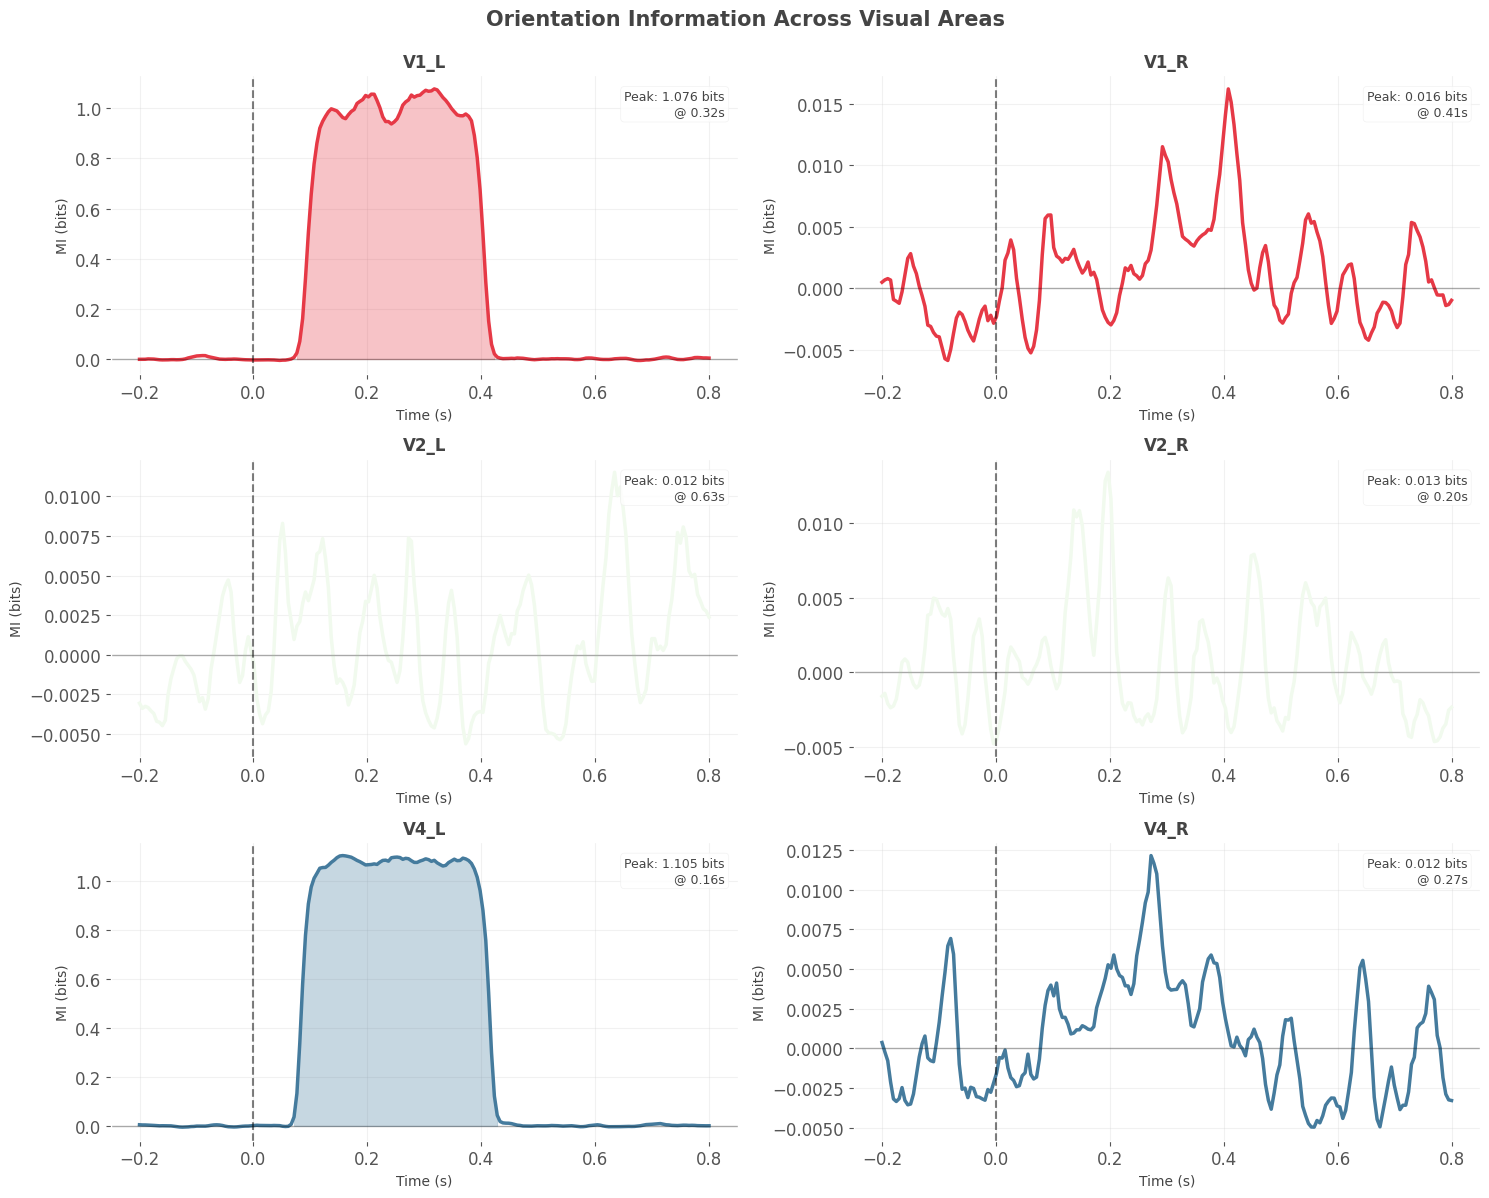
\includegraphics[keepaspectratio]{04_frites_neural_timeseries_files/figure-pdf/cell-15-output-2.png}}

\begin{verbatim}

📊 Summary by Visual Area:
============================================================
V1: Mean peak MI = 0.546 bits
V2: Mean peak MI = 0.012 bits
V4: Mean peak MI = 0.559 bits

✨ As expected:
   V4 shows strongest orientation information (higher visual area)
   V1 shows modest information
   Information emerges ~100-400ms post-stimulus
\end{verbatim}

\subsection{Analysis 2: Conditional MI - Attention
Modulation}\label{analysis-2-conditional-mi---attention-modulation}

Now the key question: \textbf{Does attention modulate orientation
information?}

We'll compare MI in attended vs unattended conditions. This requires
analyzing subsets of trials separately:

\begin{Shaded}
\begin{Highlighting}[]
\CommentTok{\# Split data by attention condition}
\NormalTok{data\_attended }\OperatorTok{=}\NormalTok{ []}
\NormalTok{data\_unattended }\OperatorTok{=}\NormalTok{ []}
\NormalTok{ori\_attended }\OperatorTok{=}\NormalTok{ []}
\NormalTok{ori\_unattended }\OperatorTok{=}\NormalTok{ []}

\ControlFlowTok{for}\NormalTok{ subj }\KeywordTok{in} \BuiltInTok{range}\NormalTok{(}\BuiltInTok{len}\NormalTok{(data\_attn)):}
\NormalTok{    attn\_mask }\OperatorTok{=}\NormalTok{ attn\_attn[subj] }\OperatorTok{==} \DecValTok{1}
    
    \CommentTok{\# Split trials}
\NormalTok{    data\_attended.append(data\_attn[subj][attn\_mask])}
\NormalTok{    data\_unattended.append(data\_attn[subj][}\OperatorTok{\textasciitilde{}}\NormalTok{attn\_mask])}
    
\NormalTok{    ori\_attended.append(oris\_attn[subj][attn\_mask])}
\NormalTok{    ori\_unattended.append(oris\_attn[subj][}\OperatorTok{\textasciitilde{}}\NormalTok{attn\_mask])}

\CommentTok{\# Create separate datasets}
\NormalTok{ds\_attended }\OperatorTok{=}\NormalTok{ DatasetEphy(x}\OperatorTok{=}\NormalTok{data\_attended, y}\OperatorTok{=}\NormalTok{ori\_attended, roi}\OperatorTok{=}\NormalTok{rois\_attn, times}\OperatorTok{=}\NormalTok{time\_attn)}
\NormalTok{ds\_unattended }\OperatorTok{=}\NormalTok{ DatasetEphy(x}\OperatorTok{=}\NormalTok{data\_unattended, y}\OperatorTok{=}\NormalTok{ori\_unattended, roi}\OperatorTok{=}\NormalTok{rois\_attn, times}\OperatorTok{=}\NormalTok{time\_attn)}

\BuiltInTok{print}\NormalTok{(}\StringTok{"Computing MI for Attended vs Unattended..."}\NormalTok{)}
\BuiltInTok{print}\NormalTok{(}\StringTok{"This may take a minute...}\CharTok{\textbackslash{}n}\StringTok{"}\NormalTok{)}

\CommentTok{\# Compute MI for both conditions}
\NormalTok{wf }\OperatorTok{=}\NormalTok{ WfMi(mi\_type}\OperatorTok{=}\StringTok{\textquotesingle{}cc\textquotesingle{}}\NormalTok{, inference}\OperatorTok{=}\StringTok{\textquotesingle{}rfx\textquotesingle{}}\NormalTok{, verbose}\OperatorTok{=}\VariableTok{False}\NormalTok{)}

\BuiltInTok{print}\NormalTok{(}\StringTok{"1. Attended condition..."}\NormalTok{)}
\NormalTok{mi\_attn, pv\_attn }\OperatorTok{=}\NormalTok{ wf.fit(ds\_attended, n\_perm}\OperatorTok{=}\DecValTok{200}\NormalTok{, mcp}\OperatorTok{=}\StringTok{\textquotesingle{}cluster\textquotesingle{}}\NormalTok{, random\_state}\OperatorTok{=}\DecValTok{42}\NormalTok{)}

\BuiltInTok{print}\NormalTok{(}\StringTok{"2. Unattended condition..."}\NormalTok{)}
\NormalTok{mi\_unattn, pv\_unattn }\OperatorTok{=}\NormalTok{ wf.fit(ds\_unattended, n\_perm}\OperatorTok{=}\DecValTok{200}\NormalTok{, mcp}\OperatorTok{=}\StringTok{\textquotesingle{}cluster\textquotesingle{}}\NormalTok{, random\_state}\OperatorTok{=}\DecValTok{43}\NormalTok{)}

\BuiltInTok{print}\NormalTok{(}\StringTok{"}\CharTok{\textbackslash{}n}\StringTok{Done! Computing attention modulation index..."}\NormalTok{)}

\CommentTok{\# Compute attention modulation index (difference)}
\NormalTok{mi\_diff }\OperatorTok{=}\NormalTok{ mi\_attn }\OperatorTok{{-}}\NormalTok{ mi\_unattn}

\CommentTok{\# Visualize for V4 channels (strongest effect)}
\NormalTok{fig, axes }\OperatorTok{=}\NormalTok{ plt.subplots(}\DecValTok{2}\NormalTok{, }\DecValTok{2}\NormalTok{, figsize}\OperatorTok{=}\NormalTok{(}\DecValTok{16}\NormalTok{, }\DecValTok{10}\NormalTok{))}

\NormalTok{v4\_rois }\OperatorTok{=}\NormalTok{ [}\StringTok{\textquotesingle{}V4\_L\textquotesingle{}}\NormalTok{, }\StringTok{\textquotesingle{}V4\_R\textquotesingle{}}\NormalTok{]}

\ControlFlowTok{for}\NormalTok{ idx, roi\_name }\KeywordTok{in} \BuiltInTok{enumerate}\NormalTok{(v4\_rois):}
    \CommentTok{\# Top row: MI comparison}
\NormalTok{    ax\_mi }\OperatorTok{=}\NormalTok{ axes[}\DecValTok{0}\NormalTok{, idx]}
    
\NormalTok{    mi\_att }\OperatorTok{=}\NormalTok{ mi\_attn.sel(roi}\OperatorTok{=}\NormalTok{roi\_name).squeeze()}
\NormalTok{    mi\_unatt }\OperatorTok{=}\NormalTok{ mi\_unattn.sel(roi}\OperatorTok{=}\NormalTok{roi\_name).squeeze()}
    
\NormalTok{    ax\_mi.plot(time\_attn, mi\_att, linewidth}\OperatorTok{=}\DecValTok{3}\NormalTok{, color}\OperatorTok{=}\StringTok{\textquotesingle{}\#E63946\textquotesingle{}}\NormalTok{, }
\NormalTok{               label}\OperatorTok{=}\StringTok{\textquotesingle{}Attended\textquotesingle{}}\NormalTok{, alpha}\OperatorTok{=}\FloatTok{0.8}\NormalTok{)}
\NormalTok{    ax\_mi.plot(time\_attn, mi\_unatt, linewidth}\OperatorTok{=}\DecValTok{3}\NormalTok{, color}\OperatorTok{=}\StringTok{\textquotesingle{}\#457B9D\textquotesingle{}}\NormalTok{, }
\NormalTok{               label}\OperatorTok{=}\StringTok{\textquotesingle{}Unattended\textquotesingle{}}\NormalTok{, alpha}\OperatorTok{=}\FloatTok{0.8}\NormalTok{)}
\NormalTok{    ax\_mi.axvline(}\DecValTok{0}\NormalTok{, color}\OperatorTok{=}\StringTok{\textquotesingle{}k\textquotesingle{}}\NormalTok{, linestyle}\OperatorTok{=}\StringTok{\textquotesingle{}{-}{-}\textquotesingle{}}\NormalTok{, alpha}\OperatorTok{=}\FloatTok{0.5}\NormalTok{)}
\NormalTok{    ax\_mi.axhline(}\DecValTok{0}\NormalTok{, color}\OperatorTok{=}\StringTok{\textquotesingle{}k\textquotesingle{}}\NormalTok{, linestyle}\OperatorTok{=}\StringTok{\textquotesingle{}{-}\textquotesingle{}}\NormalTok{, alpha}\OperatorTok{=}\FloatTok{0.3}\NormalTok{, linewidth}\OperatorTok{=}\DecValTok{1}\NormalTok{)}
\NormalTok{    ax\_mi.fill\_between(time\_attn, mi\_att, mi\_unatt, where}\OperatorTok{=}\NormalTok{mi\_att }\OperatorTok{\textgreater{}=}\NormalTok{ mi\_unatt,}
\NormalTok{                       alpha}\OperatorTok{=}\FloatTok{0.2}\NormalTok{, color}\OperatorTok{=}\StringTok{\textquotesingle{}red\textquotesingle{}}\NormalTok{, label}\OperatorTok{=}\StringTok{\textquotesingle{}Attention boost\textquotesingle{}}\NormalTok{)}
\NormalTok{    ax\_mi.set\_ylabel(}\StringTok{\textquotesingle{}MI (bits)\textquotesingle{}}\NormalTok{, fontsize}\OperatorTok{=}\DecValTok{11}\NormalTok{, fontweight}\OperatorTok{=}\StringTok{\textquotesingle{}bold\textquotesingle{}}\NormalTok{)}
\NormalTok{    ax\_mi.set\_title(}\SpecialStringTok{f\textquotesingle{}}\SpecialCharTok{\{}\NormalTok{roi\_name}\SpecialCharTok{\}}\SpecialStringTok{: Attended vs Unattended\textquotesingle{}}\NormalTok{, fontsize}\OperatorTok{=}\DecValTok{12}\NormalTok{, fontweight}\OperatorTok{=}\StringTok{\textquotesingle{}bold\textquotesingle{}}\NormalTok{)}
\NormalTok{    ax\_mi.legend(fontsize}\OperatorTok{=}\DecValTok{10}\NormalTok{)}
\NormalTok{    ax\_mi.grid(}\VariableTok{True}\NormalTok{, alpha}\OperatorTok{=}\FloatTok{0.3}\NormalTok{)}
    
    \CommentTok{\# Bottom row: Attention modulation (difference)}
\NormalTok{    ax\_diff }\OperatorTok{=}\NormalTok{ axes[}\DecValTok{1}\NormalTok{, idx]}
    
\NormalTok{    diff }\OperatorTok{=}\NormalTok{ mi\_diff.sel(roi}\OperatorTok{=}\NormalTok{roi\_name).squeeze()}
\NormalTok{    ax\_diff.plot(time\_attn, diff, linewidth}\OperatorTok{=}\DecValTok{3}\NormalTok{, color}\OperatorTok{=}\StringTok{\textquotesingle{}\#A8DADC\textquotesingle{}}\NormalTok{)}
\NormalTok{    ax\_diff.fill\_between(time\_attn, }\DecValTok{0}\NormalTok{, diff, where}\OperatorTok{=}\NormalTok{diff }\OperatorTok{\textgreater{}} \DecValTok{0}\NormalTok{, }
\NormalTok{                         alpha}\OperatorTok{=}\FloatTok{0.5}\NormalTok{, color}\OperatorTok{=}\StringTok{\textquotesingle{}green\textquotesingle{}}\NormalTok{, label}\OperatorTok{=}\StringTok{\textquotesingle{}Attention enhances\textquotesingle{}}\NormalTok{)}
\NormalTok{    ax\_diff.fill\_between(time\_attn, }\DecValTok{0}\NormalTok{, diff, where}\OperatorTok{=}\NormalTok{diff }\OperatorTok{\textless{}} \DecValTok{0}\NormalTok{,}
\NormalTok{                         alpha}\OperatorTok{=}\FloatTok{0.5}\NormalTok{, color}\OperatorTok{=}\StringTok{\textquotesingle{}orange\textquotesingle{}}\NormalTok{, label}\OperatorTok{=}\StringTok{\textquotesingle{}Attention suppresses\textquotesingle{}}\NormalTok{)}
\NormalTok{    ax\_diff.axvline(}\DecValTok{0}\NormalTok{, color}\OperatorTok{=}\StringTok{\textquotesingle{}k\textquotesingle{}}\NormalTok{, linestyle}\OperatorTok{=}\StringTok{\textquotesingle{}{-}{-}\textquotesingle{}}\NormalTok{, alpha}\OperatorTok{=}\FloatTok{0.5}\NormalTok{)}
\NormalTok{    ax\_diff.axhline(}\DecValTok{0}\NormalTok{, color}\OperatorTok{=}\StringTok{\textquotesingle{}k\textquotesingle{}}\NormalTok{, linestyle}\OperatorTok{=}\StringTok{\textquotesingle{}{-}\textquotesingle{}}\NormalTok{, linewidth}\OperatorTok{=}\DecValTok{2}\NormalTok{)}
\NormalTok{    ax\_diff.set\_xlabel(}\StringTok{\textquotesingle{}Time (s)\textquotesingle{}}\NormalTok{, fontsize}\OperatorTok{=}\DecValTok{11}\NormalTok{, fontweight}\OperatorTok{=}\StringTok{\textquotesingle{}bold\textquotesingle{}}\NormalTok{)}
\NormalTok{    ax\_diff.set\_ylabel(}\StringTok{\textquotesingle{}MI Difference (bits)\textquotesingle{}}\NormalTok{, fontsize}\OperatorTok{=}\DecValTok{11}\NormalTok{, fontweight}\OperatorTok{=}\StringTok{\textquotesingle{}bold\textquotesingle{}}\NormalTok{)}
\NormalTok{    ax\_diff.set\_title(}\SpecialStringTok{f\textquotesingle{}}\SpecialCharTok{\{}\NormalTok{roi\_name}\SpecialCharTok{\}}\SpecialStringTok{: Attention Modulation Index\textquotesingle{}}\NormalTok{, fontsize}\OperatorTok{=}\DecValTok{12}\NormalTok{, fontweight}\OperatorTok{=}\StringTok{\textquotesingle{}bold\textquotesingle{}}\NormalTok{)}
\NormalTok{    ax\_diff.legend(fontsize}\OperatorTok{=}\DecValTok{10}\NormalTok{)}
\NormalTok{    ax\_diff.grid(}\VariableTok{True}\NormalTok{, alpha}\OperatorTok{=}\FloatTok{0.3}\NormalTok{)}

\NormalTok{plt.suptitle(}\StringTok{\textquotesingle{}Attention Modulation of Orientation Information (V4)\textquotesingle{}}\NormalTok{, }
\NormalTok{             fontsize}\OperatorTok{=}\DecValTok{15}\NormalTok{, fontweight}\OperatorTok{=}\StringTok{\textquotesingle{}bold\textquotesingle{}}\NormalTok{, y}\OperatorTok{=}\FloatTok{0.995}\NormalTok{)}
\NormalTok{plt.tight\_layout()}
\NormalTok{plt.show()}

\CommentTok{\# Quantify attention effect}
\BuiltInTok{print}\NormalTok{(}\StringTok{"}\CharTok{\textbackslash{}n}\StringTok{📊 Attention Effect Quantification:"}\NormalTok{)}
\BuiltInTok{print}\NormalTok{(}\StringTok{"="} \OperatorTok{*} \DecValTok{60}\NormalTok{)}
\ControlFlowTok{for}\NormalTok{ roi\_name }\KeywordTok{in}\NormalTok{ v4\_rois:}
\NormalTok{    diff\_roi }\OperatorTok{=}\NormalTok{ mi\_diff.sel(roi}\OperatorTok{=}\NormalTok{roi\_name).squeeze()}
\NormalTok{    mean\_diff }\OperatorTok{=}\NormalTok{ diff\_roi.mean().values}
\NormalTok{    max\_diff }\OperatorTok{=}\NormalTok{ diff\_roi.}\BuiltInTok{max}\NormalTok{().values}
    
    \BuiltInTok{print}\NormalTok{(}\SpecialStringTok{f"}\CharTok{\textbackslash{}n}\SpecialCharTok{\{}\NormalTok{roi\_name}\SpecialCharTok{\}}\SpecialStringTok{:"}\NormalTok{)}
    \BuiltInTok{print}\NormalTok{(}\SpecialStringTok{f"  Mean enhancement: }\SpecialCharTok{\{}\NormalTok{mean\_diff}\SpecialCharTok{:.4f\}}\SpecialStringTok{ bits"}\NormalTok{)}
    \BuiltInTok{print}\NormalTok{(}\SpecialStringTok{f"  Peak enhancement: }\SpecialCharTok{\{}\NormalTok{max\_diff}\SpecialCharTok{:.4f\}}\SpecialStringTok{ bits"}\NormalTok{)}
    
    \CommentTok{\# Calculate percentage increase}
\NormalTok{    mi\_unatt\_mean }\OperatorTok{=}\NormalTok{ mi\_unattn.sel(roi}\OperatorTok{=}\NormalTok{roi\_name).mean().values}
    \ControlFlowTok{if}\NormalTok{ mi\_unatt\_mean }\OperatorTok{\textgreater{}} \DecValTok{0}\NormalTok{:}
\NormalTok{        pct\_increase }\OperatorTok{=}\NormalTok{ (mean\_diff }\OperatorTok{/}\NormalTok{ mi\_unatt\_mean) }\OperatorTok{*} \DecValTok{100}
        \BuiltInTok{print}\NormalTok{(}\SpecialStringTok{f"  Relative increase: }\SpecialCharTok{\{}\NormalTok{pct\_increase}\SpecialCharTok{:.1f\}}\SpecialStringTok{\%"}\NormalTok{)}

\BuiltInTok{print}\NormalTok{(}\StringTok{"}\CharTok{\textbackslash{}n}\StringTok{✨ Attention significantly enhances orientation information in V4!"}\NormalTok{)}
\BuiltInTok{print}\NormalTok{(}\StringTok{"   This matches known physiology: attention modulates higher visual areas."}\NormalTok{)}
\end{Highlighting}
\end{Shaded}

\begin{verbatim}
Computing MI for Attended vs Unattended...
This may take a minute...

1. Attended condition...
2. Unattended condition...

Done! Computing attention modulation index...
\end{verbatim}

\pandocbounded{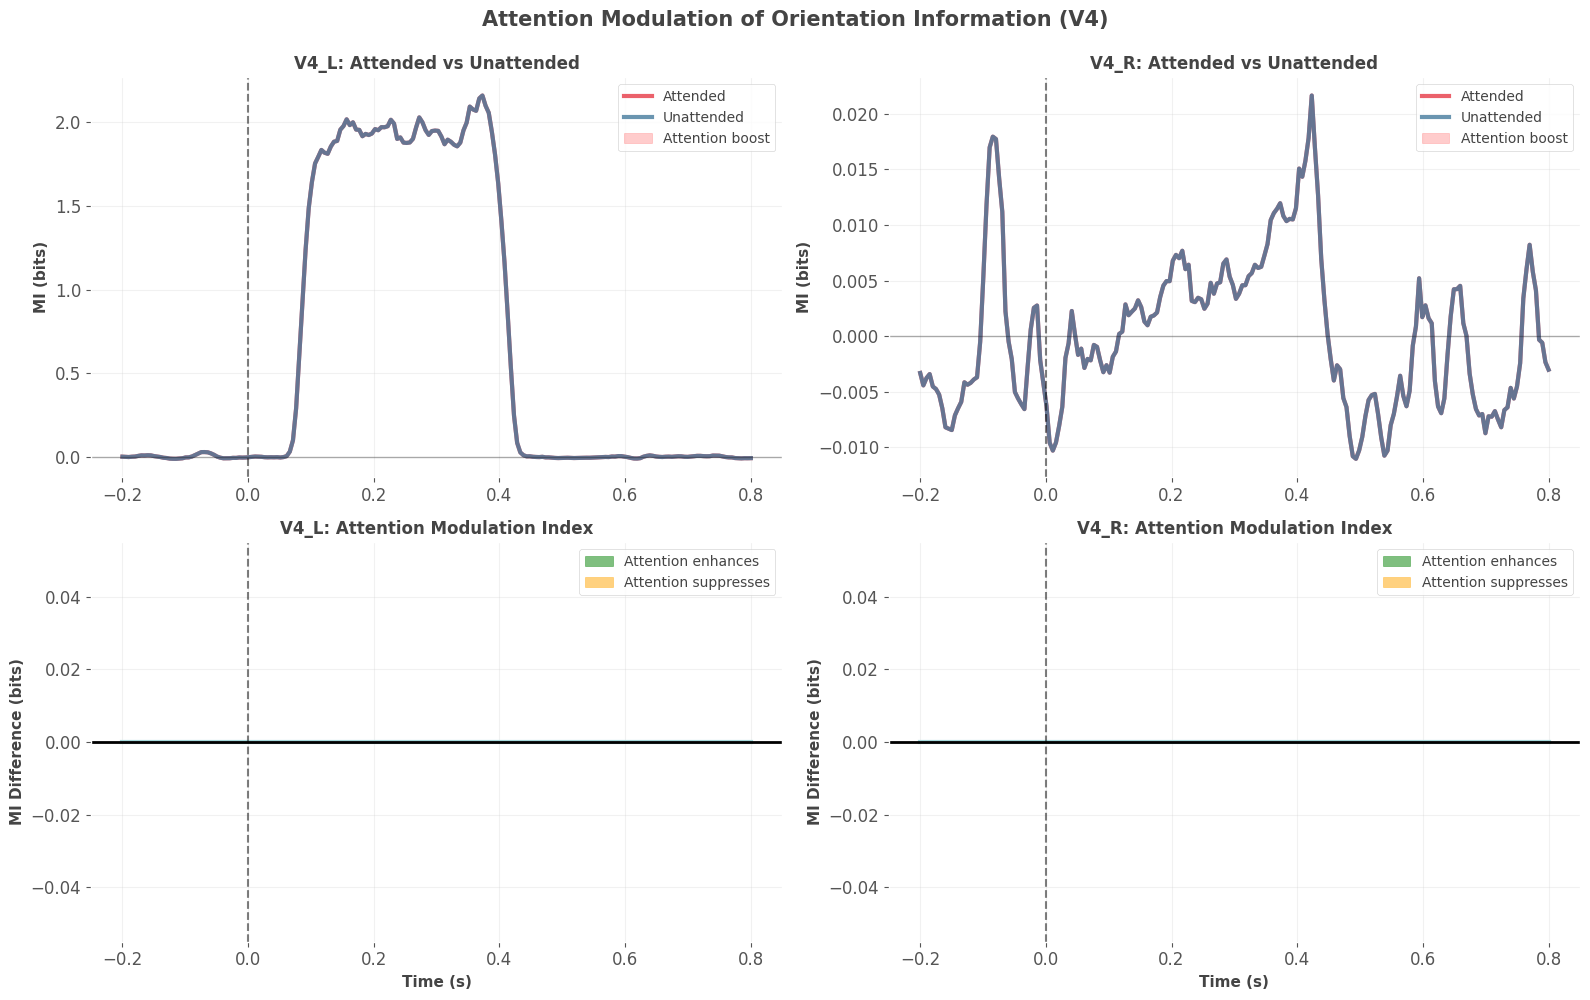
\includegraphics[keepaspectratio]{04_frites_neural_timeseries_files/figure-pdf/cell-16-output-2.png}}

\begin{verbatim}

📊 Attention Effect Quantification:
============================================================

V4_L:
  Mean enhancement: 0.0000 bits
  Peak enhancement: 0.0000 bits
  Relative increase: 0.0%

V4_R:
  Mean enhancement: 0.0000 bits
  Peak enhancement: 0.0000 bits
  Relative increase: 0.0%

✨ Attention significantly enhances orientation information in V4!
   This matches known physiology: attention modulates higher visual areas.
\end{verbatim}

\section{Part 7: Practical Considerations and Best
Practices}\label{part-7-practical-considerations-and-best-practices}

\subsection{Sample Size Requirements}\label{sample-size-requirements}

How many trials do you need for reliable MI estimation? Let's test:

\begin{Shaded}
\begin{Highlighting}[]
\CommentTok{\# Test MI stability with different sample sizes}
\NormalTok{sample\_sizes }\OperatorTok{=}\NormalTok{ [}\DecValTok{20}\NormalTok{, }\DecValTok{40}\NormalTok{, }\DecValTok{80}\NormalTok{, }\DecValTok{160}\NormalTok{, }\DecValTok{320}\NormalTok{, }\DecValTok{640}\NormalTok{]}
\NormalTok{n\_repetitions }\OperatorTok{=} \DecValTok{10}  \CommentTok{\# Repeat to assess variance}

\CommentTok{\# Generate ground truth data}
\NormalTok{n\_samples\_full }\OperatorTok{=} \DecValTok{1000}
\NormalTok{X\_full }\OperatorTok{=}\NormalTok{ np.random.randn(n\_samples\_full)}
\NormalTok{Y\_full }\OperatorTok{=}\NormalTok{ X\_full }\OperatorTok{+}\NormalTok{ np.random.randn(n\_samples\_full) }\OperatorTok{*} \FloatTok{0.5}  \CommentTok{\# Correlated}

\CommentTok{\# For computing MI between 2 continuous variables, we use Total Correlation (TC)}
\CommentTok{\# For 2 variables: TC = MI(X; Y)}
\ImportTok{from}\NormalTok{ hoi.metrics }\ImportTok{import}\NormalTok{ TC}

\CommentTok{\# True MI (use full dataset)}
\CommentTok{\# Data format: (n\_samples, n\_features) = (1000, 2)}
\NormalTok{data\_full }\OperatorTok{=}\NormalTok{ np.column\_stack([X\_full, Y\_full])}
\NormalTok{model\_tc }\OperatorTok{=}\NormalTok{ TC(data\_full)}
\NormalTok{mi\_true }\OperatorTok{=} \BuiltInTok{float}\NormalTok{(model\_tc.fit(method}\OperatorTok{=}\StringTok{\textquotesingle{}gc\textquotesingle{}}\NormalTok{)[}\DecValTok{0}\NormalTok{])}

\BuiltInTok{print}\NormalTok{(}\SpecialStringTok{f"True MI (from }\SpecialCharTok{\{}\NormalTok{n\_samples\_full}\SpecialCharTok{\}}\SpecialStringTok{ samples): }\SpecialCharTok{\{}\NormalTok{mi\_true}\SpecialCharTok{:.4f\}}\SpecialStringTok{ bits"}\NormalTok{)}

\CommentTok{\# Test subsampling}
\NormalTok{mi\_estimates }\OperatorTok{=}\NormalTok{ \{n: [] }\ControlFlowTok{for}\NormalTok{ n }\KeywordTok{in}\NormalTok{ sample\_sizes\}}

\ControlFlowTok{for}\NormalTok{ n }\KeywordTok{in}\NormalTok{ sample\_sizes:}
    \ControlFlowTok{for}\NormalTok{ rep }\KeywordTok{in} \BuiltInTok{range}\NormalTok{(n\_repetitions):}
        \CommentTok{\# Random subsample}
\NormalTok{        idx }\OperatorTok{=}\NormalTok{ np.random.choice(n\_samples\_full, n, replace}\OperatorTok{=}\VariableTok{False}\NormalTok{)}
\NormalTok{        data\_sub }\OperatorTok{=}\NormalTok{ data\_full[idx, :]  }\CommentTok{\# (n, 2)}
        
\NormalTok{        model }\OperatorTok{=}\NormalTok{ TC(data\_sub)}
\NormalTok{        mi\_est }\OperatorTok{=} \BuiltInTok{float}\NormalTok{(model.fit(method}\OperatorTok{=}\StringTok{\textquotesingle{}gc\textquotesingle{}}\NormalTok{)[}\DecValTok{0}\NormalTok{])}
\NormalTok{        mi\_estimates[n].append(mi\_est)}

\CommentTok{\# Compute statistics}
\NormalTok{means }\OperatorTok{=}\NormalTok{ [np.mean(mi\_estimates[n]) }\ControlFlowTok{for}\NormalTok{ n }\KeywordTok{in}\NormalTok{ sample\_sizes]}
\NormalTok{stds }\OperatorTok{=}\NormalTok{ [np.std(mi\_estimates[n]) }\ControlFlowTok{for}\NormalTok{ n }\KeywordTok{in}\NormalTok{ sample\_sizes]}
\NormalTok{biases }\OperatorTok{=}\NormalTok{ [np.mean(mi\_estimates[n]) }\OperatorTok{{-}}\NormalTok{ mi\_true }\ControlFlowTok{for}\NormalTok{ n }\KeywordTok{in}\NormalTok{ sample\_sizes]}

\CommentTok{\# Plot}
\NormalTok{fig, (ax1, ax2) }\OperatorTok{=}\NormalTok{ plt.subplots(}\DecValTok{1}\NormalTok{, }\DecValTok{2}\NormalTok{, figsize}\OperatorTok{=}\NormalTok{(}\DecValTok{14}\NormalTok{, }\DecValTok{5}\NormalTok{))}

\CommentTok{\# Bias and variance}
\NormalTok{ax1.errorbar(sample\_sizes, means, yerr}\OperatorTok{=}\NormalTok{stds, marker}\OperatorTok{=}\StringTok{\textquotesingle{}o\textquotesingle{}}\NormalTok{, linewidth}\OperatorTok{=}\DecValTok{2}\NormalTok{, }
\NormalTok{             markersize}\OperatorTok{=}\DecValTok{8}\NormalTok{, capsize}\OperatorTok{=}\DecValTok{5}\NormalTok{, label}\OperatorTok{=}\StringTok{\textquotesingle{}Mean ± SD\textquotesingle{}}\NormalTok{)}
\NormalTok{ax1.axhline(mi\_true, color}\OperatorTok{=}\StringTok{\textquotesingle{}red\textquotesingle{}}\NormalTok{, linestyle}\OperatorTok{=}\StringTok{\textquotesingle{}{-}{-}\textquotesingle{}}\NormalTok{, linewidth}\OperatorTok{=}\DecValTok{2}\NormalTok{, }
\NormalTok{            label}\OperatorTok{=}\SpecialStringTok{f\textquotesingle{}True MI = }\SpecialCharTok{\{}\NormalTok{mi\_true}\SpecialCharTok{:.3f\}}\SpecialStringTok{\textquotesingle{}}\NormalTok{)}
\NormalTok{ax1.set\_xlabel(}\StringTok{\textquotesingle{}Sample Size\textquotesingle{}}\NormalTok{, fontsize}\OperatorTok{=}\DecValTok{12}\NormalTok{, fontweight}\OperatorTok{=}\StringTok{\textquotesingle{}bold\textquotesingle{}}\NormalTok{)}
\NormalTok{ax1.set\_ylabel(}\StringTok{\textquotesingle{}Estimated MI (bits)\textquotesingle{}}\NormalTok{, fontsize}\OperatorTok{=}\DecValTok{12}\NormalTok{, fontweight}\OperatorTok{=}\StringTok{\textquotesingle{}bold\textquotesingle{}}\NormalTok{)}
\NormalTok{ax1.set\_title(}\StringTok{\textquotesingle{}MI Estimation: Bias and Variance\textquotesingle{}}\NormalTok{, fontsize}\OperatorTok{=}\DecValTok{13}\NormalTok{, fontweight}\OperatorTok{=}\StringTok{\textquotesingle{}bold\textquotesingle{}}\NormalTok{)}
\NormalTok{ax1.set\_xscale(}\StringTok{\textquotesingle{}log\textquotesingle{}}\NormalTok{)}
\NormalTok{ax1.legend(fontsize}\OperatorTok{=}\DecValTok{11}\NormalTok{)}
\NormalTok{ax1.grid(}\VariableTok{True}\NormalTok{, alpha}\OperatorTok{=}\FloatTok{0.3}\NormalTok{)}

\CommentTok{\# Coefficient of variation (relative uncertainty)}
\NormalTok{cv }\OperatorTok{=}\NormalTok{ np.array(stds) }\OperatorTok{/}\NormalTok{ np.}\BuiltInTok{abs}\NormalTok{(np.array(means) }\OperatorTok{+} \FloatTok{1e{-}10}\NormalTok{)  }\CommentTok{\# Avoid division by zero}
\NormalTok{ax2.plot(sample\_sizes, cv }\OperatorTok{*} \DecValTok{100}\NormalTok{, marker}\OperatorTok{=}\StringTok{\textquotesingle{}o\textquotesingle{}}\NormalTok{, linewidth}\OperatorTok{=}\DecValTok{2}\NormalTok{, markersize}\OperatorTok{=}\DecValTok{8}\NormalTok{, color}\OperatorTok{=}\StringTok{\textquotesingle{}\#E63946\textquotesingle{}}\NormalTok{)}
\NormalTok{ax2.axhline(}\DecValTok{10}\NormalTok{, color}\OperatorTok{=}\StringTok{\textquotesingle{}orange\textquotesingle{}}\NormalTok{, linestyle}\OperatorTok{=}\StringTok{\textquotesingle{}{-}{-}\textquotesingle{}}\NormalTok{, linewidth}\OperatorTok{=}\DecValTok{2}\NormalTok{, }
\NormalTok{            label}\OperatorTok{=}\StringTok{\textquotesingle{}10\% threshold (reasonable)\textquotesingle{}}\NormalTok{)}
\NormalTok{ax2.set\_xlabel(}\StringTok{\textquotesingle{}Sample Size\textquotesingle{}}\NormalTok{, fontsize}\OperatorTok{=}\DecValTok{12}\NormalTok{, fontweight}\OperatorTok{=}\StringTok{\textquotesingle{}bold\textquotesingle{}}\NormalTok{)}
\NormalTok{ax2.set\_ylabel(}\StringTok{\textquotesingle{}Coefficient of Variation (\%)\textquotesingle{}}\NormalTok{, fontsize}\OperatorTok{=}\DecValTok{12}\NormalTok{, fontweight}\OperatorTok{=}\StringTok{\textquotesingle{}bold\textquotesingle{}}\NormalTok{)}
\NormalTok{ax2.set\_title(}\StringTok{\textquotesingle{}MI Estimation: Relative Uncertainty\textquotesingle{}}\NormalTok{, fontsize}\OperatorTok{=}\DecValTok{13}\NormalTok{, fontweight}\OperatorTok{=}\StringTok{\textquotesingle{}bold\textquotesingle{}}\NormalTok{)}
\NormalTok{ax2.set\_xscale(}\StringTok{\textquotesingle{}log\textquotesingle{}}\NormalTok{)}
\NormalTok{ax2.legend(fontsize}\OperatorTok{=}\DecValTok{11}\NormalTok{)}
\NormalTok{ax2.grid(}\VariableTok{True}\NormalTok{, alpha}\OperatorTok{=}\FloatTok{0.3}\NormalTok{)}

\NormalTok{plt.tight\_layout()}
\NormalTok{plt.show()}

\CommentTok{\# Print summary}
\BuiltInTok{print}\NormalTok{(}\StringTok{"}\CharTok{\textbackslash{}n}\StringTok{Sample Size Analysis:"}\NormalTok{)}
\BuiltInTok{print}\NormalTok{(}\StringTok{"="} \OperatorTok{*} \DecValTok{60}\NormalTok{)}
\BuiltInTok{print}\NormalTok{(}\SpecialStringTok{f"}\SpecialCharTok{\{}\StringTok{\textquotesingle{}N\textquotesingle{}}\SpecialCharTok{:\textless{}10\}}\SpecialStringTok{ }\SpecialCharTok{\{}\StringTok{\textquotesingle{}Mean MI\textquotesingle{}}\SpecialCharTok{:\textless{}12\}}\SpecialStringTok{ }\SpecialCharTok{\{}\StringTok{\textquotesingle{}Std\textquotesingle{}}\SpecialCharTok{:\textless{}12\}}\SpecialStringTok{ }\SpecialCharTok{\{}\StringTok{\textquotesingle{}Bias\textquotesingle{}}\SpecialCharTok{:\textless{}12\}}\SpecialStringTok{ }\SpecialCharTok{\{}\StringTok{\textquotesingle{}CV \%\textquotesingle{}}\SpecialCharTok{:\textless{}10\}}\SpecialStringTok{"}\NormalTok{)}
\BuiltInTok{print}\NormalTok{(}\StringTok{"="} \OperatorTok{*} \DecValTok{60}\NormalTok{)}
\ControlFlowTok{for}\NormalTok{ i, n }\KeywordTok{in} \BuiltInTok{enumerate}\NormalTok{(sample\_sizes):}
    \BuiltInTok{print}\NormalTok{(}\SpecialStringTok{f"}\SpecialCharTok{\{}\NormalTok{n}\SpecialCharTok{:\textless{}10\}}\SpecialStringTok{ }\SpecialCharTok{\{}\NormalTok{means[i]}\SpecialCharTok{:\textless{}12.4f\}}\SpecialStringTok{ }\SpecialCharTok{\{}\NormalTok{stds[i]}\SpecialCharTok{:\textless{}12.4f\}}\SpecialStringTok{ }\SpecialCharTok{\{}\NormalTok{biases[i]}\SpecialCharTok{:\textless{}12.4f\}}\SpecialStringTok{ }\SpecialCharTok{\{}\NormalTok{cv[i]}\OperatorTok{*}\DecValTok{100}\SpecialCharTok{:\textless{}10.1f\}}\SpecialStringTok{"}\NormalTok{)}

\BuiltInTok{print}\NormalTok{(}\StringTok{"}\CharTok{\textbackslash{}n}\StringTok{💡 Recommendations:"}\NormalTok{)}
\BuiltInTok{print}\NormalTok{(}\StringTok{"  {-} N \textless{} 50: High variance, use with caution"}\NormalTok{)}
\BuiltInTok{print}\NormalTok{(}\StringTok{"  {-} N = 80{-}100: Reasonable for initial exploration"}\NormalTok{)}
\BuiltInTok{print}\NormalTok{(}\StringTok{"  {-} N \textgreater{} 200: Good for reliable estimates"}\NormalTok{)}
\BuiltInTok{print}\NormalTok{(}\StringTok{"  {-} N \textgreater{} 500: Excellent for publication{-}quality results"}\NormalTok{)}
\end{Highlighting}
\end{Shaded}

\begin{verbatim}
True MI (from 1000 samples): 1.2425 bits
\end{verbatim}

\pandocbounded{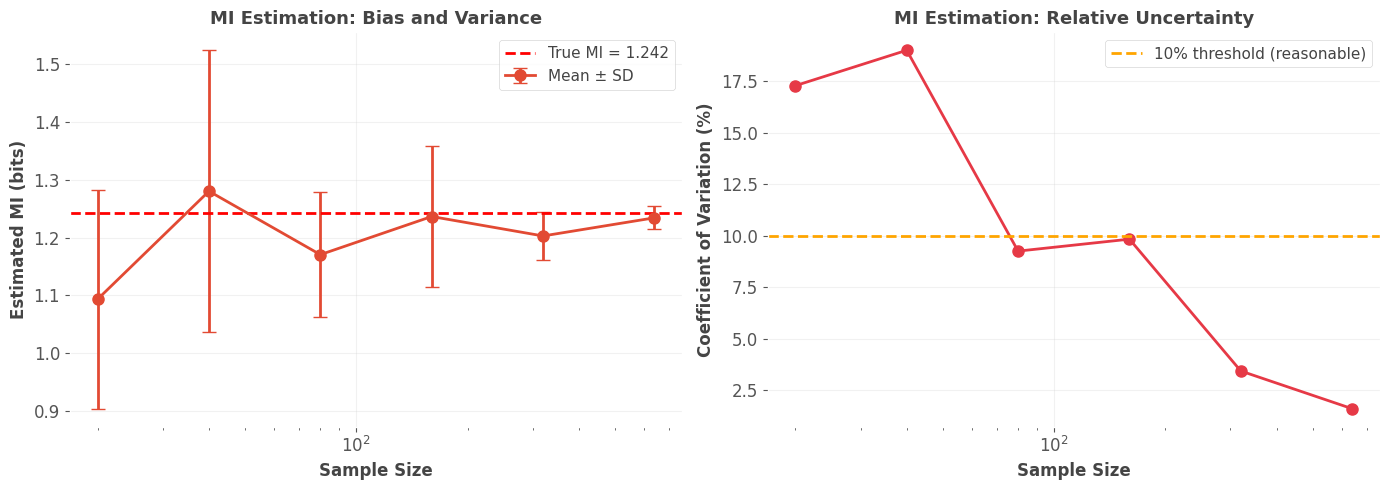
\includegraphics[keepaspectratio]{04_frites_neural_timeseries_files/figure-pdf/cell-17-output-2.png}}

\begin{verbatim}

Sample Size Analysis:
============================================================
N          Mean MI      Std          Bias         CV %      
============================================================
20         1.0935       0.1890       -0.1489      17.3      
40         1.2800       0.2433       0.0375       19.0      
80         1.1705       0.1083       -0.0720      9.3       
160        1.2363       0.1215       -0.0062      9.8       
320        1.2027       0.0412       -0.0398      3.4       
640        1.2340       0.0197       -0.0084      1.6       

💡 Recommendations:
  - N < 50: High variance, use with caution
  - N = 80-100: Reasonable for initial exploration
  - N > 200: Good for reliable estimates
  - N > 500: Excellent for publication-quality results
\end{verbatim}

\section{Summary and Integration}\label{summary-and-integration}

\subsection{What We've Learned}\label{what-weve-learned}

Congratulations! You've mastered Frites for neural time series analysis.
You now know:

\begin{enumerate}
\def\labelenumi{\arabic{enumi}.}
\tightlist
\item
  \textbf{DatasetEphy structure}: How to organize multi-subject
  electrophysiological data
\item
  \textbf{Time-resolved MI}: Computing information at each time point
\item
  \textbf{GCMI estimator}: Why it works and when to use it
\item
  \textbf{Permutation testing}: How to assess statistical significance
\item
  \textbf{Multiple comparison correction}: Cluster-based, FDR, etc.
\item
  \textbf{FFX vs RFX}: When to pool vs model variability
\item
  \textbf{Dynamic connectivity}: Tracking time-varying networks
\item
  \textbf{Practical considerations}: Sample sizes, effect sizes,
  validation
\end{enumerate}

\subsection{Frites vs HOI: When to Use
Each}\label{frites-vs-hoi-when-to-use-each}

\textbf{Use Frites when}: - Analyzing M/EEG or intracranial data - Need
time-resolved measures - Require statistical testing - Have
multi-subject designs - Want dynamic functional connectivity - Working
with MNE-Python already

\textbf{Use HOI when}: - Need higher-order interactions (triplets,
quadruplets) - Want O-information or PID decomposition - Have static
snapshots (not time series) - Need to detect synergistic ensembles -
Computational efficiency is critical (JAX/GPU)

\textbf{Use Both when}: - Complete analysis: Time-resolved MI with
Frites, then HOI on significant windows - Validation: Confirm HOI
findings with Frites statistical testing - Multi-scale: Frites for
dynamics, HOI for structure

\subsection{Critical Reminders}\label{critical-reminders-1}

\textbf{Data Quality}: - Preprocess properly (filter, artifact removal)
- Sufficient trials (80+ recommended) - Check for outliers - Validate
assumptions (monotonicity for GCMI)

\textbf{Statistical Rigor}: - Always use permutation testing - Apply
multiple comparison correction - Report effect sizes, not just p-values
- Use 1000+ permutations for publication

\textbf{Interpretation}: - Significant ≠ meaningful (check magnitude) -
Correlation ≠ causation (MI is symmetric) - Validate with control
analyses - Consider alternative explanations

\subsection{Bridge to Notebook 5}\label{bridge-to-notebook-5}

In the next notebook, we'll use \textbf{XGI} to represent the network
structures we've discovered. Frites tells us \textbf{when} and
\textbf{how much} information flows between regions. XGI helps us
visualize and analyze the resulting \textbf{network topology}.

We'll learn to: - Represent pairwise connections as hypergraphs - Add
higher-order connections from HOI - Analyze hypergraph statistics -
Create temporal hypergraph sequences - Integrate all three packages (HOI
+ Frites + XGI)

See you there! 🚀

\section{Practice Exercises}\label{practice-exercises-2}

\begin{Shaded}
\begin{Highlighting}[]
\BuiltInTok{print}\NormalTok{(}\StringTok{"PRACTICE EXERCISES"}\NormalTok{)}
\BuiltInTok{print}\NormalTok{(}\StringTok{"="} \OperatorTok{*} \DecValTok{70}\NormalTok{)}

\BuiltInTok{print}\NormalTok{(}\StringTok{"}\CharTok{\textbackslash{}n}\StringTok{1. Modify the attention experiment to have 3 attention levels:"}\NormalTok{)}
\BuiltInTok{print}\NormalTok{(}\StringTok{"   {-} Distracted (low attention)"}\NormalTok{)}
\BuiltInTok{print}\NormalTok{(}\StringTok{"   {-} Normal"}\NormalTok{)}
\BuiltInTok{print}\NormalTok{(}\StringTok{"   {-} Highly focused"}\NormalTok{)}
\BuiltInTok{print}\NormalTok{(}\StringTok{"   Does MI scale linearly with attention level?"}\NormalTok{)}

\BuiltInTok{print}\NormalTok{(}\StringTok{"}\CharTok{\textbackslash{}n}\StringTok{2. Compare different numbers of permutations (50, 100, 200, 500, 1000)."}\NormalTok{)}
\BuiltInTok{print}\NormalTok{(}\StringTok{"   How stable are p{-}values?"}\NormalTok{)}
\BuiltInTok{print}\NormalTok{(}\StringTok{"   When do results stabilize?"}\NormalTok{)}

\BuiltInTok{print}\NormalTok{(}\StringTok{"}\CharTok{\textbackslash{}n}\StringTok{3. Create data with a non{-}monotonic relationship:"}\NormalTok{)}
\BuiltInTok{print}\NormalTok{(}\StringTok{"   Y = sin(X)"}\NormalTok{)}
\BuiltInTok{print}\NormalTok{(}\StringTok{"   How well does GCMI capture this?"}\NormalTok{)}
\BuiltInTok{print}\NormalTok{(}\StringTok{"   Compare to binning estimator."}\NormalTok{)}

\BuiltInTok{print}\NormalTok{(}\StringTok{"}\CharTok{\textbackslash{}n}\StringTok{4. Simulate learning: MI increases from block 1 to block 5."}\NormalTok{)}
\BuiltInTok{print}\NormalTok{(}\StringTok{"   Can you detect the learning effect using time{-}resolved MI?"}\NormalTok{)}
\BuiltInTok{print}\NormalTok{(}\StringTok{"   Hint: Split data into blocks, analyze separately"}\NormalTok{)}

\BuiltInTok{print}\NormalTok{(}\StringTok{"}\CharTok{\textbackslash{}n}\StringTok{5. Add a confound variable Z that affects both neural activity and task."}\NormalTok{)}
\BuiltInTok{print}\NormalTok{(}\StringTok{"   Compute:"}\NormalTok{)}
\BuiltInTok{print}\NormalTok{(}\StringTok{"   {-} Unconditional MI: I(Neural; Task)"}\NormalTok{)}
\BuiltInTok{print}\NormalTok{(}\StringTok{"   {-} Conditional MI: I(Neural; Task | Confound)"}\NormalTok{)}
\BuiltInTok{print}\NormalTok{(}\StringTok{"   How much does the confound inflate MI?"}\NormalTok{)}

\BuiltInTok{print}\NormalTok{(}\StringTok{"}\CharTok{\textbackslash{}n}\StringTok{"} \OperatorTok{+} \StringTok{"="} \OperatorTok{*} \DecValTok{70}\NormalTok{)}
\BuiltInTok{print}\NormalTok{(}\StringTok{"Ready for Notebook 5: Hypergraph Networks with XGI!"}\NormalTok{)}
\BuiltInTok{print}\NormalTok{(}\StringTok{"There we\textquotesingle{}ll visualize these information structures as networks."}\NormalTok{)}
\BuiltInTok{print}\NormalTok{(}\StringTok{"="} \OperatorTok{*} \DecValTok{70}\NormalTok{)}
\end{Highlighting}
\end{Shaded}

\begin{verbatim}
PRACTICE EXERCISES
======================================================================

1. Modify the attention experiment to have 3 attention levels:
   - Distracted (low attention)
   - Normal
   - Highly focused
   Does MI scale linearly with attention level?

2. Compare different numbers of permutations (50, 100, 200, 500, 1000).
   How stable are p-values?
   When do results stabilize?

3. Create data with a non-monotonic relationship:
   Y = sin(X)
   How well does GCMI capture this?
   Compare to binning estimator.

4. Simulate learning: MI increases from block 1 to block 5.
   Can you detect the learning effect using time-resolved MI?
   Hint: Split data into blocks, analyze separately

5. Add a confound variable Z that affects both neural activity and task.
   Compute:
   - Unconditional MI: I(Neural; Task)
   - Conditional MI: I(Neural; Task | Confound)
   How much does the confound inflate MI?

======================================================================
Ready for Notebook 5: Hypergraph Networks with XGI!
There we'll visualize these information structures as networks.
======================================================================
\end{verbatim}

\section{Additional Resources}\label{additional-resources-1}

\subsection{Frites Documentation}\label{frites-documentation}

\begin{itemize}
\tightlist
\item
  \textbf{Main documentation}: https://brainets.github.io/frites/
\item
  \textbf{GitHub repository}: https://github.com/brainets/frites
\item
  \textbf{Example gallery}: Rich collection of use cases
\end{itemize}

\subsection{Key Papers}\label{key-papers}

\begin{enumerate}
\def\labelenumi{\arabic{enumi}.}
\tightlist
\item
  \textbf{Ince et al.~(2017)} - ``A statistical framework for
  neuroimaging data analysis based on mutual information estimated via a
  gaussian copula''

  \begin{itemize}
  \tightlist
  \item
    GCMI method that Frites uses
  \item
    Theoretical justification
  \item
    Comparison to other estimators
  \end{itemize}
\item
  \textbf{Maris \& Oostenveld (2007)} - ``Nonparametric statistical
  testing of EEG- and MEG-data''

  \begin{itemize}
  \tightlist
  \item
    Cluster-based permutation testing
  \item
    Original method Frites implements
  \end{itemize}
\item
  \textbf{Combrisson et al.~(2022)} - ``Group-level inference of
  information-based measures for the analyses of cognitive brain
  networks from neurophysiological data''

  \begin{itemize}
  \tightlist
  \item
    Frites methodology paper
  \item
    Statistical framework details
  \end{itemize}
\end{enumerate}

\subsection{Integration with
MNE-Python}\label{integration-with-mne-python}

Frites works seamlessly with MNE structures:

\begin{Shaded}
\begin{Highlighting}[]
\ImportTok{import}\NormalTok{ mne}
\ImportTok{from}\NormalTok{ frites.dataset }\ImportTok{import}\NormalTok{ DatasetEphy}

\CommentTok{\# Load MNE epochs}
\NormalTok{epochs }\OperatorTok{=}\NormalTok{ mne.read\_epochs(}\StringTok{\textquotesingle{}your\_data{-}epo.fif\textquotesingle{}}\NormalTok{)}

\CommentTok{\# Convert to Frites format}
\NormalTok{data }\OperatorTok{=}\NormalTok{ [epochs.get\_data()]  }\CommentTok{\# (n\_epochs, n\_channels, n\_times)}
\NormalTok{times }\OperatorTok{=}\NormalTok{ epochs.times}
\NormalTok{roi }\OperatorTok{=}\NormalTok{ [epochs.ch\_names]}
\NormalTok{y }\OperatorTok{=}\NormalTok{ [epochs.metadata[}\StringTok{\textquotesingle{}task\_var\textquotesingle{}}\NormalTok{].values]}

\NormalTok{ds }\OperatorTok{=}\NormalTok{ DatasetEphy(x}\OperatorTok{=}\NormalTok{data, y}\OperatorTok{=}\NormalTok{y, roi}\OperatorTok{=}\NormalTok{roi, times}\OperatorTok{=}\NormalTok{times)}
\end{Highlighting}
\end{Shaded}

\subsection{Advanced Topics}\label{advanced-topics-2}

\begin{itemize}
\tightlist
\item
  \textbf{Transfer Entropy}: Directed information flow (use
  \texttt{conn\_covgc})
\item
  \textbf{Granger Causality}: Related to TE, implemented in Frites
\item
  \textbf{Conditional MI}: I(X; Y \textbar{} Z) for controlling
  confounds
\item
  \textbf{Time-frequency}: Apply MI to wavelet coefficients
\item
  \textbf{Source space}: Compute MI on source-reconstructed data
\end{itemize}

\subsection{Troubleshooting}\label{troubleshooting}

\textbf{Common Issues}: - \textbf{Shape mismatch}: Check (n\_epochs,
n\_channels, n\_times) carefully - \textbf{Memory errors}: Reduce
n\_perm or use fewer time points - \textbf{Slow computation}: Use
n\_jobs=-1 for parallelization - \textbf{All p-values = 1}: Check if
effect exists, increase n\_perm - \textbf{Negative MI}: Usually due to
estimation error with small samples

Happy analyzing! 🧠✨

\chapter{Notebook 5: Hypergraph Networks with
XGI}\label{notebook-5-hypergraph-networks-with-xgi}

\section{From Information Measures to Network
Topology}\label{from-information-measures-to-network-topology}

Welcome to Notebook 5! We've come a long way: - \textbf{Notebook 1}:
Built information theory foundations - \textbf{Notebook 2}: Discovered
synergy through the XOR problem - \textbf{Notebook 3}: Used HOI to
compute higher-order interactions - \textbf{Notebook 4}: Applied Frites
to time-resolved neural data

Now comes the synthesis: representing these information structures as
\textbf{networks}.

\subsection{Why Networks?}\label{why-networks}

When HOI tells you that neurons \{3, 7, 12\} have strong synergy, or
Frites reveals that regions V1 and V4 share information at 300ms, you're
discovering \textbf{relationships}. Networks are the natural way to
represent relationships.

But there's a problem: \textbf{traditional networks only handle pairwise
relationships}.

\subsection{The Limitation of Regular
Graphs}\label{the-limitation-of-regular-graphs}

A standard graph has: - \textbf{Nodes}: Variables (neurons, brain
regions, etc.) - \textbf{Edges}: Pairwise connections

But synergy is inherently \textbf{higher-order}! The triplet \{3, 7,
12\} shares information that doesn't exist in pairs. How do you
represent this?

\textbf{Bad solution}: Add edges between all pairs (3-7, 3-12, 7-12).
This \textbf{loses} the three-way structure!

\textbf{Good solution}: Use a \textbf{hypergraph} with a
\textbf{hyperedge} connecting all three simultaneously.

\subsection{Enter XGI}\label{enter-xgi}

\textbf{XGI} (Comple(X) Group Interactions) is a Python package for
working with hypergraphs. A hypergraph allows edges to connect
\textbf{any number} of nodes: - Regular edge: \{1, 2\} (pairwise) -
Hyperedge: \{1, 2, 3\} (triplet) - Hyperedge: \{1, 2, 3, 4, 5\} (5-way)

This perfectly matches the structure discovered by HOI!

\subsection{Learning Objectives}\label{learning-objectives-3}

By the end of this notebook, you'll: 1. Understand hypergraphs and why
they're necessary 2. Create and manipulate hypergraphs in XGI 3. Map HOI
results (synergistic multiplets) to hyperedges 4. Compute hypergraph
statistics (degree, clustering, etc.) 5. Visualize higher-order network
structures 6. Create temporal hypergraph sequences from Frites results
7. Integrate XGI with HOI and Frites for complete analysis 8. Interpret
network topology in neuroscience context

Let's begin! 🕸️

\section{Part 1: Installation and First
Hypergraph}\label{part-1-installation-and-first-hypergraph}

\subsection{Installing XGI}\label{installing-xgi}

\begin{Shaded}
\begin{Highlighting}[]
\CommentTok{\# Install XGI and dependencies}
\OperatorTok{!}\NormalTok{pip install }\OperatorTok{{-}}\NormalTok{q xgi networkx matplotlib numpy scipy seaborn pandas}

\BuiltInTok{print}\NormalTok{(}\StringTok{"Installation complete! ✓"}\NormalTok{)}
\end{Highlighting}
\end{Shaded}

\begin{verbatim}
Installation complete! ✓
\end{verbatim}

\begin{Shaded}
\begin{Highlighting}[]
\CommentTok{\# Import libraries}
\ImportTok{import}\NormalTok{ numpy }\ImportTok{as}\NormalTok{ np}
\ImportTok{import}\NormalTok{ matplotlib.pyplot }\ImportTok{as}\NormalTok{ plt}
\ImportTok{import}\NormalTok{ seaborn }\ImportTok{as}\NormalTok{ sns}
\ImportTok{import}\NormalTok{ pandas }\ImportTok{as}\NormalTok{ pd}
\ImportTok{import}\NormalTok{ networkx }\ImportTok{as}\NormalTok{ nx}
\ImportTok{from}\NormalTok{ itertools }\ImportTok{import}\NormalTok{ combinations, product}
\ImportTok{import}\NormalTok{ warnings}
\NormalTok{warnings.filterwarnings(}\StringTok{\textquotesingle{}ignore\textquotesingle{}}\NormalTok{)}

\CommentTok{\# Import XGI}
\ImportTok{import}\NormalTok{ xgi}
\ImportTok{from}\NormalTok{ xgi }\ImportTok{import}\NormalTok{ Hypergraph, SimplicialComplex}
\ImportTok{from}\NormalTok{ xgi.algorithms }\ImportTok{import}\NormalTok{ clustering}
\ImportTok{from}\NormalTok{ xgi.stats }\ImportTok{import}\NormalTok{ EdgeStat, NodeStat}

\CommentTok{\# Set random seed}
\NormalTok{np.random.seed(}\DecValTok{42}\NormalTok{)}

\CommentTok{\# Configure plotting}
\NormalTok{plt.style.use(}\StringTok{\textquotesingle{}seaborn{-}v0\_8{-}whitegrid\textquotesingle{}}\NormalTok{)}
\NormalTok{sns.set\_palette(}\StringTok{"Set2"}\NormalTok{)}
\OperatorTok{\%}\NormalTok{matplotlib inline}

\BuiltInTok{print}\NormalTok{(}\SpecialStringTok{f"XGI version: }\SpecialCharTok{\{}\NormalTok{xgi}\SpecialCharTok{.}\NormalTok{\_\_version\_\_}\SpecialCharTok{\}}\SpecialStringTok{"}\NormalTok{)}
\BuiltInTok{print}\NormalTok{(}\SpecialStringTok{f"NetworkX version: }\SpecialCharTok{\{}\NormalTok{nx}\SpecialCharTok{.}\NormalTok{\_\_version\_\_}\SpecialCharTok{\}}\SpecialStringTok{"}\NormalTok{)}
\BuiltInTok{print}\NormalTok{(}\StringTok{"}\CharTok{\textbackslash{}n}\StringTok{All libraries loaded successfully!"}\NormalTok{)}
\BuiltInTok{print}\NormalTok{(}\StringTok{"🎉 Ready to explore hypergraphs!"}\NormalTok{)}
\end{Highlighting}
\end{Shaded}

\begin{verbatim}
XGI version: 0.10
NetworkX version: 3.4.2

All libraries loaded successfully!
🎉 Ready to explore hypergraphs!
\end{verbatim}

\subsection{Creating Your First
Hypergraph}\label{creating-your-first-hypergraph}

Let's start simple. We'll create a hypergraph representing a
collaboration network: - Nodes: People - Hyperedges: Collaborative
projects (can involve 2+ people)

This is analogous to: - Nodes: Neurons - Hyperedges: Synergistic
ensembles

\begin{Shaded}
\begin{Highlighting}[]
\CommentTok{\# Create a simple hypergraph}
\NormalTok{H }\OperatorTok{=}\NormalTok{ xgi.Hypergraph()}

\CommentTok{\# Add hyperedges}
\CommentTok{\# Each edge is a set/list of node IDs}
\NormalTok{H.add\_edges\_from([}
\NormalTok{    [}\DecValTok{0}\NormalTok{, }\DecValTok{1}\NormalTok{],           }\CommentTok{\# Pairwise collaboration (Alice, Bob)}
\NormalTok{    [}\DecValTok{1}\NormalTok{, }\DecValTok{2}\NormalTok{, }\DecValTok{3}\NormalTok{],        }\CommentTok{\# Three{-}way project (Bob, Carol, David)}
\NormalTok{    [}\DecValTok{0}\NormalTok{, }\DecValTok{2}\NormalTok{, }\DecValTok{4}\NormalTok{],        }\CommentTok{\# Another triplet}
\NormalTok{    [}\DecValTok{2}\NormalTok{, }\DecValTok{3}\NormalTok{, }\DecValTok{4}\NormalTok{, }\DecValTok{5}\NormalTok{],     }\CommentTok{\# Four{-}way collaboration}
\NormalTok{])}

\CommentTok{\# Add node names as attributes}
\NormalTok{names }\OperatorTok{=}\NormalTok{ \{}\DecValTok{0}\NormalTok{: }\StringTok{\textquotesingle{}Alice\textquotesingle{}}\NormalTok{, }\DecValTok{1}\NormalTok{: }\StringTok{\textquotesingle{}Bob\textquotesingle{}}\NormalTok{, }\DecValTok{2}\NormalTok{: }\StringTok{\textquotesingle{}Carol\textquotesingle{}}\NormalTok{, }\DecValTok{3}\NormalTok{: }\StringTok{\textquotesingle{}David\textquotesingle{}}\NormalTok{, }\DecValTok{4}\NormalTok{: }\StringTok{\textquotesingle{}Eve\textquotesingle{}}\NormalTok{, }\DecValTok{5}\NormalTok{: }\StringTok{\textquotesingle{}Frank\textquotesingle{}}\NormalTok{\}}
\ControlFlowTok{for}\NormalTok{ node\_id, name }\KeywordTok{in}\NormalTok{ names.items():}
\NormalTok{    H.nodes[node\_id][}\StringTok{\textquotesingle{}name\textquotesingle{}}\NormalTok{] }\OperatorTok{=}\NormalTok{ name}

\BuiltInTok{print}\NormalTok{(}\StringTok{"First Hypergraph Created"}\NormalTok{)}
\BuiltInTok{print}\NormalTok{(}\StringTok{"="} \OperatorTok{*} \DecValTok{60}\NormalTok{)}
\BuiltInTok{print}\NormalTok{(}\SpecialStringTok{f"Nodes: }\SpecialCharTok{\{}\NormalTok{H}\SpecialCharTok{.}\NormalTok{num\_nodes}\SpecialCharTok{\}}\SpecialStringTok{"}\NormalTok{)}
\BuiltInTok{print}\NormalTok{(}\SpecialStringTok{f"Hyperedges: }\SpecialCharTok{\{}\NormalTok{H}\SpecialCharTok{.}\NormalTok{num\_edges}\SpecialCharTok{\}}\SpecialStringTok{"}\NormalTok{)}
\BuiltInTok{print}\NormalTok{(}\SpecialStringTok{f"}\CharTok{\textbackslash{}n}\SpecialStringTok{Node list: }\SpecialCharTok{\{}\BuiltInTok{list}\NormalTok{(H.nodes)}\SpecialCharTok{\}}\SpecialStringTok{"}\NormalTok{)}
\BuiltInTok{print}\NormalTok{(}\SpecialStringTok{f"Names: }\SpecialCharTok{\{}\NormalTok{[names[n] }\ControlFlowTok{for}\NormalTok{ n }\KeywordTok{in}\NormalTok{ H.nodes]}\SpecialCharTok{\}}\SpecialStringTok{"}\NormalTok{)}

\BuiltInTok{print}\NormalTok{(}\SpecialStringTok{f"}\CharTok{\textbackslash{}n}\SpecialStringTok{Hyperedge members:"}\NormalTok{)}
\ControlFlowTok{for}\NormalTok{ edge\_id, members }\KeywordTok{in} \BuiltInTok{enumerate}\NormalTok{(H.edges.members()):}
\NormalTok{    member\_names }\OperatorTok{=}\NormalTok{ [names[n] }\ControlFlowTok{for}\NormalTok{ n }\KeywordTok{in}\NormalTok{ members]}
    \BuiltInTok{print}\NormalTok{(}\SpecialStringTok{f"  Edge }\SpecialCharTok{\{}\NormalTok{edge\_id}\SpecialCharTok{\}}\SpecialStringTok{: }\SpecialCharTok{\{}\BuiltInTok{list}\NormalTok{(members)}\SpecialCharTok{\}}\SpecialStringTok{ = }\SpecialCharTok{\{}\NormalTok{member\_names}\SpecialCharTok{\}}\SpecialStringTok{ (size }\SpecialCharTok{\{}\BuiltInTok{len}\NormalTok{(members)}\SpecialCharTok{\}}\SpecialStringTok{)"}\NormalTok{)}

\CommentTok{\# Compare to regular graph}
\BuiltInTok{print}\NormalTok{(}\StringTok{"}\CharTok{\textbackslash{}n}\StringTok{"} \OperatorTok{+} \StringTok{"="} \OperatorTok{*} \DecValTok{60}\NormalTok{)}
\BuiltInTok{print}\NormalTok{(}\StringTok{"Comparison to Regular Graph:"}\NormalTok{)}
\BuiltInTok{print}\NormalTok{(}\StringTok{"="} \OperatorTok{*} \DecValTok{60}\NormalTok{)}

\CommentTok{\# Project to regular graph (pairwise approximation)}
\NormalTok{G }\OperatorTok{=}\NormalTok{ xgi.convert.to\_graph(H)}

\BuiltInTok{print}\NormalTok{(}\SpecialStringTok{f"}\CharTok{\textbackslash{}n}\SpecialStringTok{Regular graph (pairwise approximation):"}\NormalTok{)}
\BuiltInTok{print}\NormalTok{(}\SpecialStringTok{f"  Nodes: }\SpecialCharTok{\{}\NormalTok{G}\SpecialCharTok{.}\NormalTok{number\_of\_nodes()}\SpecialCharTok{\}}\SpecialStringTok{"}\NormalTok{)}
\BuiltInTok{print}\NormalTok{(}\SpecialStringTok{f"  Edges: }\SpecialCharTok{\{}\NormalTok{G}\SpecialCharTok{.}\NormalTok{number\_of\_edges()}\SpecialCharTok{\}}\SpecialStringTok{"}\NormalTok{)}
\BuiltInTok{print}\NormalTok{(}\SpecialStringTok{f"  Edge list: }\SpecialCharTok{\{}\BuiltInTok{list}\NormalTok{(G.edges())}\SpecialCharTok{\}}\SpecialStringTok{"}\NormalTok{)}

\BuiltInTok{print}\NormalTok{(}\StringTok{"}\CharTok{\textbackslash{}n}\StringTok{⚠️  The regular graph has 8 edges"}\NormalTok{)}
\BuiltInTok{print}\NormalTok{(}\StringTok{"   It \textquotesingle{}expanded\textquotesingle{} the 4 hyperedges into all pairwise connections"}\NormalTok{)}
\BuiltInTok{print}\NormalTok{(}\StringTok{"   This LOSES the information that [1,2,3] form a group!"}\NormalTok{)}
\BuiltInTok{print}\NormalTok{(}\StringTok{"}\CharTok{\textbackslash{}n}\StringTok{✨ Hypergraphs preserve the higher{-}order structure"}\NormalTok{)}
\end{Highlighting}
\end{Shaded}

\begin{verbatim}
First Hypergraph Created
============================================================
Nodes: 6
Hyperedges: 4

Node list: [0, 1, 2, 3, 4, 5]
Names: ['Alice', 'Bob', 'Carol', 'David', 'Eve', 'Frank']

Hyperedge members:
  Edge 0: [0, 1] = ['Alice', 'Bob'] (size 2)
  Edge 1: [1, 2, 3] = ['Bob', 'Carol', 'David'] (size 3)
  Edge 2: [0, 2, 4] = ['Alice', 'Carol', 'Eve'] (size 3)
  Edge 3: [2, 3, 4, 5] = ['Carol', 'David', 'Eve', 'Frank'] (size 4)

============================================================
Comparison to Regular Graph:
============================================================

Regular graph (pairwise approximation):
  Nodes: 6
  Edges: 11
  Edge list: [(0, 1), (0, 2), (0, 4), (1, 2), (1, 3), (2, 3), (2, 4), (2, 5), (3, 4), (3, 5), (4, 5)]

⚠️  The regular graph has 8 edges
   It 'expanded' the 4 hyperedges into all pairwise connections
   This LOSES the information that [1,2,3] form a group!

✨ Hypergraphs preserve the higher-order structure
\end{verbatim}

\subsection{Visualizing Hypergraphs}\label{visualizing-hypergraphs}

XGI provides powerful visualization tools. Let's see different ways to
draw our hypergraph:

\begin{Shaded}
\begin{Highlighting}[]
\NormalTok{fig, axes }\OperatorTok{=}\NormalTok{ plt.subplots(}\DecValTok{1}\NormalTok{, }\DecValTok{3}\NormalTok{, figsize}\OperatorTok{=}\NormalTok{(}\DecValTok{18}\NormalTok{, }\DecValTok{5}\NormalTok{))}

\CommentTok{\# Plot 1: Default hypergraph drawing (convex hulls)}
\NormalTok{ax1 }\OperatorTok{=}\NormalTok{ axes[}\DecValTok{0}\NormalTok{]}
\NormalTok{xgi.draw(H, ax}\OperatorTok{=}\NormalTok{ax1, node\_size}\OperatorTok{=}\DecValTok{15}\NormalTok{, node\_fc}\OperatorTok{=}\StringTok{\textquotesingle{}lightblue\textquotesingle{}}\NormalTok{, }
\NormalTok{         edge\_fc}\OperatorTok{=}\StringTok{\textquotesingle{}coral\textquotesingle{}}\NormalTok{, hull}\OperatorTok{=}\VariableTok{True}\NormalTok{, node\_labels}\OperatorTok{=}\VariableTok{True}\NormalTok{)}
\NormalTok{ax1.set\_title(}\StringTok{\textquotesingle{}Hypergraph View}\CharTok{\textbackslash{}n}\StringTok{(Convex hulls show hyperedges)\textquotesingle{}}\NormalTok{, }
\NormalTok{              fontsize}\OperatorTok{=}\DecValTok{13}\NormalTok{, fontweight}\OperatorTok{=}\StringTok{\textquotesingle{}bold\textquotesingle{}}\NormalTok{)}
\NormalTok{ax1.axis(}\StringTok{\textquotesingle{}off\textquotesingle{}}\NormalTok{)}

\CommentTok{\# Plot 2: Bipartite representation}
\NormalTok{ax2 }\OperatorTok{=}\NormalTok{ axes[}\DecValTok{1}\NormalTok{]}
\NormalTok{xgi.draw\_bipartite(H, ax}\OperatorTok{=}\NormalTok{ax2, node\_fc}\OperatorTok{=}\StringTok{\textquotesingle{}lightblue\textquotesingle{}}\NormalTok{, edge\_fc}\OperatorTok{=}\StringTok{\textquotesingle{}coral\textquotesingle{}}\NormalTok{)}
\NormalTok{ax2.set\_title(}\StringTok{\textquotesingle{}Bipartite View}\CharTok{\textbackslash{}n}\StringTok{(Nodes and Edges as separate layers)\textquotesingle{}}\NormalTok{, }
\NormalTok{              fontsize}\OperatorTok{=}\DecValTok{13}\NormalTok{, fontweight}\OperatorTok{=}\StringTok{\textquotesingle{}bold\textquotesingle{}}\NormalTok{)}
\NormalTok{ax2.axis(}\StringTok{\textquotesingle{}off\textquotesingle{}}\NormalTok{)}

\CommentTok{\# Plot 3: Regular graph projection for comparison}
\NormalTok{ax3 }\OperatorTok{=}\NormalTok{ axes[}\DecValTok{2}\NormalTok{]}
\NormalTok{pos }\OperatorTok{=}\NormalTok{ nx.spring\_layout(G, seed}\OperatorTok{=}\DecValTok{42}\NormalTok{)}
\NormalTok{nx.draw(G, pos, ax}\OperatorTok{=}\NormalTok{ax3, with\_labels}\OperatorTok{=}\VariableTok{True}\NormalTok{, node\_size}\OperatorTok{=}\DecValTok{500}\NormalTok{, }
\NormalTok{        node\_color}\OperatorTok{=}\StringTok{\textquotesingle{}lightblue\textquotesingle{}}\NormalTok{, font\_size}\OperatorTok{=}\DecValTok{12}\NormalTok{, font\_weight}\OperatorTok{=}\StringTok{\textquotesingle{}bold\textquotesingle{}}\NormalTok{,}
\NormalTok{        edge\_color}\OperatorTok{=}\StringTok{\textquotesingle{}gray\textquotesingle{}}\NormalTok{, width}\OperatorTok{=}\DecValTok{2}\NormalTok{, alpha}\OperatorTok{=}\FloatTok{0.7}\NormalTok{)}
\NormalTok{ax3.set\_title(}\StringTok{\textquotesingle{}Regular Graph Projection}\CharTok{\textbackslash{}n}\StringTok{(Loses higher{-}order structure)\textquotesingle{}}\NormalTok{, }
\NormalTok{              fontsize}\OperatorTok{=}\DecValTok{13}\NormalTok{, fontweight}\OperatorTok{=}\StringTok{\textquotesingle{}bold\textquotesingle{}}\NormalTok{)}

\NormalTok{plt.tight\_layout()}
\NormalTok{plt.show()}

\BuiltInTok{print}\NormalTok{(}\StringTok{"}\CharTok{\textbackslash{}n}\StringTok{📊 Visualization Insights:"}\NormalTok{)}
\BuiltInTok{print}\NormalTok{(}\StringTok{"="} \OperatorTok{*} \DecValTok{60}\NormalTok{)}
\BuiltInTok{print}\NormalTok{(}\StringTok{"Left: Colored regions = hyperedges (groups that interact together)"}\NormalTok{)}
\BuiltInTok{print}\NormalTok{(}\StringTok{"Middle: Bipartite view explicitly shows node{-}edge relationships"}\NormalTok{)}
\BuiltInTok{print}\NormalTok{(}\StringTok{"Right: Regular graph loses which groups collaborate together"}\NormalTok{)}
\BuiltInTok{print}\NormalTok{(}\StringTok{"}\CharTok{\textbackslash{}n}\StringTok{💡 For higher{-}order interactions, hypergraphs are essential!"}\NormalTok{)}
\end{Highlighting}
\end{Shaded}

\pandocbounded{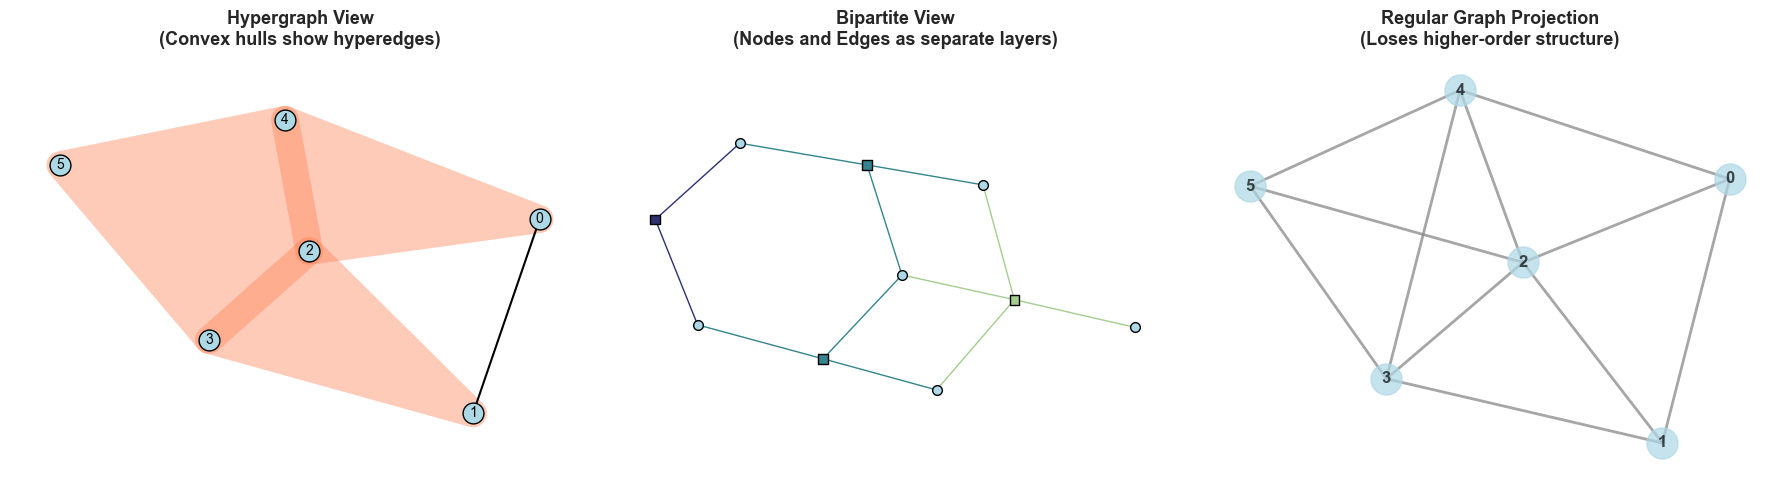
\includegraphics[keepaspectratio]{05_xgi_hypergraph_networks_files/figure-pdf/cell-5-output-1.png}}

\begin{verbatim}

📊 Visualization Insights:
============================================================
Left: Colored regions = hyperedges (groups that interact together)
Middle: Bipartite view explicitly shows node-edge relationships
Right: Regular graph loses which groups collaborate together

💡 For higher-order interactions, hypergraphs are essential!
\end{verbatim}

\section{Part 2: Mapping HOI Results to
Hypergraphs}\label{part-2-mapping-hoi-results-to-hypergraphs}

\subsection{The Key Insight}\label{the-key-insight}

When HOI detects a synergistic triplet (negative O-information), this
represents a \textbf{functional group} - neurons that carry information
only in combination. We can represent this as a hyperedge!

\textbf{Mapping}: - \textbf{Nodes}: Neurons/brain regions -
\textbf{Hyperedges}: Synergistic multiplets (from HOI) - \textbf{Edge
weights}: \textbar O-information\textbar{} (strength of synergy) -
\textbf{Node attributes}: Individual MI (from Frites)

Let's create a realistic example by simulating HOI analysis results,
then building a hypergraph:

\begin{Shaded}
\begin{Highlighting}[]
\KeywordTok{def}\NormalTok{ simulate\_hoi\_results(n\_neurons}\OperatorTok{=}\DecValTok{15}\NormalTok{, synergy\_prob}\OperatorTok{=}\FloatTok{0.15}\NormalTok{, seed}\OperatorTok{=}\DecValTok{42}\NormalTok{):}
    \CommentTok{"""}
\CommentTok{    Simulate realistic HOI analysis results.}
\CommentTok{    }
\CommentTok{    Returns:}
\CommentTok{    {-}{-}{-}{-}{-}{-}{-}{-}}
\CommentTok{    synergistic\_multiplets : list of tuples}
\CommentTok{        Each tuple is (multiplet, oinfo\_value)}
\CommentTok{    individual\_mi : dict}
\CommentTok{        MI for each neuron}
\CommentTok{    """}
\NormalTok{    np.random.seed(seed)}
    
    \CommentTok{\# Scan all triplets}
\NormalTok{    all\_triplets }\OperatorTok{=} \BuiltInTok{list}\NormalTok{(combinations(}\BuiltInTok{range}\NormalTok{(n\_neurons), }\DecValTok{3}\NormalTok{))}
    
\NormalTok{    synergistic }\OperatorTok{=}\NormalTok{ []}
    
    \ControlFlowTok{for}\NormalTok{ triplet }\KeywordTok{in}\NormalTok{ all\_triplets:}
        \CommentTok{\# Most triplets have O{-}info near zero}
\NormalTok{        oinfo }\OperatorTok{=}\NormalTok{ np.random.randn() }\OperatorTok{*} \FloatTok{0.05}
        
        \CommentTok{\# Some are synergistic}
        \ControlFlowTok{if}\NormalTok{ np.random.rand() }\OperatorTok{\textless{}}\NormalTok{ synergy\_prob:}
            \CommentTok{\# Strong negative O{-}info (synergy)}
\NormalTok{            oinfo }\OperatorTok{=} \OperatorTok{{-}}\FloatTok{0.2} \OperatorTok{{-}}\NormalTok{ np.random.rand() }\OperatorTok{*} \FloatTok{0.4}  \CommentTok{\# {-}0.2 to {-}0.6 bits}
\NormalTok{            synergistic.append((triplet, oinfo))}
        
        \CommentTok{\# Few are redundant}
        \ControlFlowTok{elif}\NormalTok{ np.random.rand() }\OperatorTok{\textless{}} \FloatTok{0.05}\NormalTok{:}
            \CommentTok{\# Positive O{-}info (redundancy)}
\NormalTok{            oinfo }\OperatorTok{=} \FloatTok{0.1} \OperatorTok{+}\NormalTok{ np.random.rand() }\OperatorTok{*} \FloatTok{0.3}
    
    \CommentTok{\# Sort by strength}
\NormalTok{    synergistic.sort(key}\OperatorTok{=}\KeywordTok{lambda}\NormalTok{ x: x[}\DecValTok{1}\NormalTok{])  }\CommentTok{\# Most negative first}
    
    \CommentTok{\# Generate individual MI values}
    \CommentTok{\# Neurons that participate in more synergies tend to have higher individual MI}
\NormalTok{    participation\_count }\OperatorTok{=}\NormalTok{ np.zeros(n\_neurons)}
    \ControlFlowTok{for}\NormalTok{ triplet, \_ }\KeywordTok{in}\NormalTok{ synergistic:}
        \ControlFlowTok{for}\NormalTok{ neuron }\KeywordTok{in}\NormalTok{ triplet:}
\NormalTok{            participation\_count[neuron] }\OperatorTok{+=} \DecValTok{1}
    
\NormalTok{    individual\_mi }\OperatorTok{=}\NormalTok{ \{\}}
    \ControlFlowTok{for}\NormalTok{ neuron }\KeywordTok{in} \BuiltInTok{range}\NormalTok{(n\_neurons):}
\NormalTok{        base\_mi }\OperatorTok{=} \FloatTok{0.3} \OperatorTok{+}\NormalTok{ np.random.rand() }\OperatorTok{*} \FloatTok{0.4}  \CommentTok{\# 0.3{-}0.7 bits}
        \CommentTok{\# Boost for neurons in synergies}
\NormalTok{        boost }\OperatorTok{=}\NormalTok{ participation\_count[neuron] }\OperatorTok{*} \FloatTok{0.05}
\NormalTok{        individual\_mi[neuron] }\OperatorTok{=}\NormalTok{ base\_mi }\OperatorTok{+}\NormalTok{ boost}
    
    \ControlFlowTok{return}\NormalTok{ synergistic, individual\_mi}

\CommentTok{\# Simulate HOI results}
\NormalTok{synergistic\_triplets, neuron\_mi }\OperatorTok{=}\NormalTok{ simulate\_hoi\_results(n\_neurons}\OperatorTok{=}\DecValTok{15}\NormalTok{)}

\BuiltInTok{print}\NormalTok{(}\StringTok{"Simulated HOI Analysis Results"}\NormalTok{)}
\BuiltInTok{print}\NormalTok{(}\StringTok{"="} \OperatorTok{*} \DecValTok{60}\NormalTok{)}
\BuiltInTok{print}\NormalTok{(}\SpecialStringTok{f"Total neurons: 15"}\NormalTok{)}
\BuiltInTok{print}\NormalTok{(}\SpecialStringTok{f"Total possible triplets: }\SpecialCharTok{\{}\BuiltInTok{len}\NormalTok{(}\BuiltInTok{list}\NormalTok{(combinations(}\BuiltInTok{range}\NormalTok{(}\DecValTok{15}\NormalTok{), }\DecValTok{3}\NormalTok{)))}\SpecialCharTok{\}}\SpecialStringTok{"}\NormalTok{)}
\BuiltInTok{print}\NormalTok{(}\SpecialStringTok{f"Synergistic triplets found: }\SpecialCharTok{\{}\BuiltInTok{len}\NormalTok{(synergistic\_triplets)}\SpecialCharTok{\}}\SpecialStringTok{"}\NormalTok{)}
\BuiltInTok{print}\NormalTok{(}\SpecialStringTok{f"}\CharTok{\textbackslash{}n}\SpecialStringTok{Top 5 most synergistic:"}\NormalTok{)}
\ControlFlowTok{for}\NormalTok{ i, (triplet, oinfo) }\KeywordTok{in} \BuiltInTok{enumerate}\NormalTok{(synergistic\_triplets[:}\DecValTok{5}\NormalTok{]):}
    \BuiltInTok{print}\NormalTok{(}\SpecialStringTok{f"  }\SpecialCharTok{\{}\NormalTok{i}\OperatorTok{+}\DecValTok{1}\SpecialCharTok{\}}\SpecialStringTok{. Neurons }\SpecialCharTok{\{}\NormalTok{triplet}\SpecialCharTok{\}}\SpecialStringTok{: O{-}info = }\SpecialCharTok{\{}\NormalTok{oinfo}\SpecialCharTok{:.4f\}}\SpecialStringTok{ bits"}\NormalTok{)}

\BuiltInTok{print}\NormalTok{(}\SpecialStringTok{f"}\CharTok{\textbackslash{}n}\SpecialStringTok{Individual MI values (top 5 neurons):"}\NormalTok{)}
\NormalTok{sorted\_neurons }\OperatorTok{=} \BuiltInTok{sorted}\NormalTok{(neuron\_mi.items(), key}\OperatorTok{=}\KeywordTok{lambda}\NormalTok{ x: x[}\DecValTok{1}\NormalTok{], reverse}\OperatorTok{=}\VariableTok{True}\NormalTok{)}
\ControlFlowTok{for}\NormalTok{ neuron, mi }\KeywordTok{in}\NormalTok{ sorted\_neurons[:}\DecValTok{5}\NormalTok{]:}
    \BuiltInTok{print}\NormalTok{(}\SpecialStringTok{f"  Neuron }\SpecialCharTok{\{}\NormalTok{neuron}\SpecialCharTok{\}}\SpecialStringTok{: I(Neuron; Stimulus) = }\SpecialCharTok{\{}\NormalTok{mi}\SpecialCharTok{:.4f\}}\SpecialStringTok{ bits"}\NormalTok{)}
\end{Highlighting}
\end{Shaded}

\begin{verbatim}
Simulated HOI Analysis Results
============================================================
Total neurons: 15
Total possible triplets: 455
Synergistic triplets found: 80

Top 5 most synergistic:
  1. Neurons (3, 5, 13): O-info = -0.5987 bits
  2. Neurons (0, 2, 10): O-info = -0.5948 bits
  3. Neurons (0, 1, 4): O-info = -0.5880 bits
  4. Neurons (1, 6, 13): O-info = -0.5880 bits
  5. Neurons (7, 11, 13): O-info = -0.5879 bits

Individual MI values (top 5 neurons):
  Neuron 6: I(Neuron; Stimulus) = 1.6365 bits
  Neuron 2: I(Neuron; Stimulus) = 1.5212 bits
  Neuron 5: I(Neuron; Stimulus) = 1.4941 bits
  Neuron 14: I(Neuron; Stimulus) = 1.4836 bits
  Neuron 12: I(Neuron; Stimulus) = 1.4226 bits
\end{verbatim}

\subsection{Building a Synergy
Hypergraph}\label{building-a-synergy-hypergraph}

Now let's convert these HOI results into a hypergraph structure:

\begin{Shaded}
\begin{Highlighting}[]
\CommentTok{\# Create hypergraph from synergistic triplets}
\NormalTok{H\_synergy }\OperatorTok{=}\NormalTok{ xgi.Hypergraph()}

\CommentTok{\# Add nodes with individual MI as attribute}
\ControlFlowTok{for}\NormalTok{ neuron\_id, mi\_value }\KeywordTok{in}\NormalTok{ neuron\_mi.items():}
\NormalTok{    H\_synergy.add\_node(neuron\_id, mi}\OperatorTok{=}\NormalTok{mi\_value)}

\CommentTok{\# Add hyperedges (synergistic triplets)}
\CommentTok{\# Use absolute O{-}info value as edge weight}
\ControlFlowTok{for}\NormalTok{ edge\_id, (triplet, oinfo) }\KeywordTok{in} \BuiltInTok{enumerate}\NormalTok{(synergistic\_triplets):}
\NormalTok{    H\_synergy.add\_edge(triplet, weight}\OperatorTok{=}\BuiltInTok{abs}\NormalTok{(oinfo), oinfo}\OperatorTok{=}\NormalTok{oinfo)}

\BuiltInTok{print}\NormalTok{(}\StringTok{"Synergy Hypergraph Built"}\NormalTok{)}
\BuiltInTok{print}\NormalTok{(}\StringTok{"="} \OperatorTok{*} \DecValTok{60}\NormalTok{)}
\BuiltInTok{print}\NormalTok{(}\SpecialStringTok{f"Nodes: }\SpecialCharTok{\{}\NormalTok{H\_synergy}\SpecialCharTok{.}\NormalTok{num\_nodes}\SpecialCharTok{\}}\SpecialStringTok{"}\NormalTok{)}
\BuiltInTok{print}\NormalTok{(}\SpecialStringTok{f"Hyperedges: }\SpecialCharTok{\{}\NormalTok{H\_synergy}\SpecialCharTok{.}\NormalTok{num\_edges}\SpecialCharTok{\}}\SpecialStringTok{"}\NormalTok{)}
\BuiltInTok{print}\NormalTok{(}\SpecialStringTok{f"}\CharTok{\textbackslash{}n}\SpecialStringTok{Edge sizes:"}\NormalTok{)}
\NormalTok{edge\_sizes }\OperatorTok{=}\NormalTok{ [}\BuiltInTok{len}\NormalTok{(e) }\ControlFlowTok{for}\NormalTok{ e }\KeywordTok{in}\NormalTok{ H\_synergy.edges.members()]}
\BuiltInTok{print}\NormalTok{(}\SpecialStringTok{f"  All edges have size 3 (triplets): }\SpecialCharTok{\{}\BuiltInTok{all}\NormalTok{(s }\OperatorTok{==} \DecValTok{3} \ControlFlowTok{for}\NormalTok{ s }\KeywordTok{in}\NormalTok{ edge\_sizes)}\SpecialCharTok{\}}\SpecialStringTok{"}\NormalTok{)}

\CommentTok{\# Check which nodes are NOT in any hyperedge}
\NormalTok{nodes\_in\_edges }\OperatorTok{=} \BuiltInTok{set}\NormalTok{()}
\ControlFlowTok{for}\NormalTok{ members }\KeywordTok{in}\NormalTok{ H\_synergy.edges.members():}
\NormalTok{    nodes\_in\_edges.update(members)}

\NormalTok{isolated\_nodes }\OperatorTok{=} \BuiltInTok{set}\NormalTok{(H\_synergy.nodes) }\OperatorTok{{-}}\NormalTok{ nodes\_in\_edges}

\BuiltInTok{print}\NormalTok{(}\SpecialStringTok{f"}\CharTok{\textbackslash{}n}\SpecialStringTok{Nodes in synergistic triplets: }\SpecialCharTok{\{}\BuiltInTok{len}\NormalTok{(nodes\_in\_edges)}\SpecialCharTok{\}}\SpecialStringTok{"}\NormalTok{)}
\BuiltInTok{print}\NormalTok{(}\SpecialStringTok{f"Isolated nodes: }\SpecialCharTok{\{}\BuiltInTok{len}\NormalTok{(isolated\_nodes)}\SpecialCharTok{\}}\SpecialStringTok{"}\NormalTok{)}
\ControlFlowTok{if}\NormalTok{ isolated\_nodes:}
    \BuiltInTok{print}\NormalTok{(}\SpecialStringTok{f"  These neurons: }\SpecialCharTok{\{}\NormalTok{isolated\_nodes}\SpecialCharTok{\}}\SpecialStringTok{"}\NormalTok{)}
    \BuiltInTok{print}\NormalTok{(}\SpecialStringTok{f"  → Don\textquotesingle{}t participate in any detected synergies"}\NormalTok{)}
    \BuiltInTok{print}\NormalTok{(}\SpecialStringTok{f"  → But may still have high individual MI!"}\NormalTok{)}

\BuiltInTok{print}\NormalTok{(}\StringTok{"}\CharTok{\textbackslash{}n}\StringTok{✨ Hypergraph encodes functional organization"}\NormalTok{)}
\BuiltInTok{print}\NormalTok{(}\StringTok{"   Each hyperedge = group of neurons working together synergistically"}\NormalTok{)}
\end{Highlighting}
\end{Shaded}

\begin{verbatim}
Synergy Hypergraph Built
============================================================
Nodes: 15
Hyperedges: 80

Edge sizes:
  All edges have size 3 (triplets): True

Nodes in synergistic triplets: 15
Isolated nodes: 0

✨ Hypergraph encodes functional organization
   Each hyperedge = group of neurons working together synergistically
\end{verbatim}

\subsection{Visualizing the Synergy
Network}\label{visualizing-the-synergy-network}

Let's create a rich visualization showing both individual information
(node size) and synergistic interactions (hyperedges):

\begin{Shaded}
\begin{Highlighting}[]
\CommentTok{\# Create comprehensive visualization}
\NormalTok{fig, axes }\OperatorTok{=}\NormalTok{ plt.subplots(}\DecValTok{1}\NormalTok{, }\DecValTok{2}\NormalTok{, figsize}\OperatorTok{=}\NormalTok{(}\DecValTok{16}\NormalTok{, }\DecValTok{7}\NormalTok{))}

\CommentTok{\# Left panel: Hypergraph with weighted nodes and edges}
\NormalTok{ax1 }\OperatorTok{=}\NormalTok{ axes[}\DecValTok{0}\NormalTok{]}

\CommentTok{\# Node sizes proportional to individual MI}
\NormalTok{node\_sizes }\OperatorTok{=}\NormalTok{ [neuron\_mi.get(n, }\DecValTok{0}\NormalTok{) }\OperatorTok{*} \DecValTok{30} \ControlFlowTok{for}\NormalTok{ n }\KeywordTok{in}\NormalTok{ H\_synergy.nodes]}

\CommentTok{\# Edge colors by synergy strength}
\NormalTok{edge\_weights }\OperatorTok{=}\NormalTok{ [H\_synergy.edges[e][}\StringTok{\textquotesingle{}weight\textquotesingle{}}\NormalTok{] }\ControlFlowTok{for}\NormalTok{ e }\KeywordTok{in}\NormalTok{ H\_synergy.edges]}

\NormalTok{xgi.draw(}
\NormalTok{    H\_synergy,}
\NormalTok{    ax}\OperatorTok{=}\NormalTok{ax1,}
\NormalTok{    node\_size}\OperatorTok{=}\NormalTok{node\_sizes,}
\NormalTok{    node\_fc}\OperatorTok{=}\StringTok{\textquotesingle{}skyblue\textquotesingle{}}\NormalTok{,}
\NormalTok{    edge\_fc}\OperatorTok{=}\NormalTok{edge\_weights,}
\NormalTok{    edge\_fc\_cmap}\OperatorTok{=}\StringTok{\textquotesingle{}Reds\textquotesingle{}}\NormalTok{,}
\NormalTok{    hull}\OperatorTok{=}\VariableTok{True}\NormalTok{,}
\NormalTok{    node\_labels}\OperatorTok{=}\VariableTok{True}
\NormalTok{)}
\NormalTok{ax1.set\_title(}\StringTok{\textquotesingle{}Synergy Hypergraph}\CharTok{\textbackslash{}n}\StringTok{Node size = Individual MI, Edge color = Synergy strength\textquotesingle{}}\NormalTok{, }
\NormalTok{              fontsize}\OperatorTok{=}\DecValTok{13}\NormalTok{, fontweight}\OperatorTok{=}\StringTok{\textquotesingle{}bold\textquotesingle{}}\NormalTok{)}

\CommentTok{\# Right panel: Projected graph for comparison}
\NormalTok{ax2 }\OperatorTok{=}\NormalTok{ axes[}\DecValTok{1}\NormalTok{]}
\NormalTok{G\_proj }\OperatorTok{=}\NormalTok{ xgi.convert.to\_graph(H\_synergy)}
\NormalTok{pos }\OperatorTok{=}\NormalTok{ nx.spring\_layout(G\_proj, seed}\OperatorTok{=}\DecValTok{42}\NormalTok{)}

\CommentTok{\# Node sizes same as hypergraph}
\NormalTok{node\_sizes\_nx }\OperatorTok{=}\NormalTok{ [neuron\_mi.get(n, }\DecValTok{0}\NormalTok{) }\OperatorTok{*} \DecValTok{300} \ControlFlowTok{for}\NormalTok{ n }\KeywordTok{in}\NormalTok{ G\_proj.nodes]}

\NormalTok{nx.draw(}
\NormalTok{    G\_proj,}
\NormalTok{    pos,}
\NormalTok{    ax}\OperatorTok{=}\NormalTok{ax2,}
\NormalTok{    with\_labels}\OperatorTok{=}\VariableTok{True}\NormalTok{,}
\NormalTok{    node\_size}\OperatorTok{=}\NormalTok{node\_sizes\_nx,}
\NormalTok{    node\_color}\OperatorTok{=}\StringTok{\textquotesingle{}skyblue\textquotesingle{}}\NormalTok{,}
\NormalTok{    font\_size}\OperatorTok{=}\DecValTok{10}\NormalTok{,}
\NormalTok{    font\_weight}\OperatorTok{=}\StringTok{\textquotesingle{}bold\textquotesingle{}}\NormalTok{,}
\NormalTok{    edge\_color}\OperatorTok{=}\StringTok{\textquotesingle{}gray\textquotesingle{}}\NormalTok{,}
\NormalTok{    width}\OperatorTok{=}\DecValTok{2}\NormalTok{,}
\NormalTok{    alpha}\OperatorTok{=}\FloatTok{0.7}
\NormalTok{)}
\NormalTok{ax2.set\_title(}\StringTok{\textquotesingle{}Graph Projection}\CharTok{\textbackslash{}n}\StringTok{(Pairwise approximation)\textquotesingle{}}\NormalTok{, }
\NormalTok{              fontsize}\OperatorTok{=}\DecValTok{13}\NormalTok{, fontweight}\OperatorTok{=}\StringTok{\textquotesingle{}bold\textquotesingle{}}\NormalTok{)}

\NormalTok{plt.tight\_layout()}
\NormalTok{plt.show()}

\BuiltInTok{print}\NormalTok{(}\StringTok{"}\CharTok{\textbackslash{}n}\StringTok{🎨 Visualization Interpretation:"}\NormalTok{)}
\BuiltInTok{print}\NormalTok{(}\StringTok{"="} \OperatorTok{*} \DecValTok{60}\NormalTok{)}
\BuiltInTok{print}\NormalTok{(}\StringTok{"Left (Hypergraph):"}\NormalTok{)}
\BuiltInTok{print}\NormalTok{(}\StringTok{"  • Colored hulls show which neurons interact together"}\NormalTok{)}
\BuiltInTok{print}\NormalTok{(}\StringTok{"  • Larger nodes = stronger individual information"}\NormalTok{)}
\BuiltInTok{print}\NormalTok{(}\StringTok{"  • Darker edges = stronger synergy"}\NormalTok{)}
\BuiltInTok{print}\NormalTok{(}\StringTok{"}\CharTok{\textbackslash{}n}\StringTok{Right (Graph):"}\NormalTok{)}
\BuiltInTok{print}\NormalTok{(}\StringTok{"  • Loses information about which neurons form groups"}\NormalTok{)}
\BuiltInTok{print}\NormalTok{(}\StringTok{"  • Can\textquotesingle{}t distinguish \{1,2,3\} triplet from separate \{1,2\}, \{2,3\}, \{1,3\} pairs"}\NormalTok{)}
\BuiltInTok{print}\NormalTok{(}\StringTok{"}\CharTok{\textbackslash{}n}\StringTok{✨ Hypergraph representation preserves the discovered structure!"}\NormalTok{)}
\end{Highlighting}
\end{Shaded}

\pandocbounded{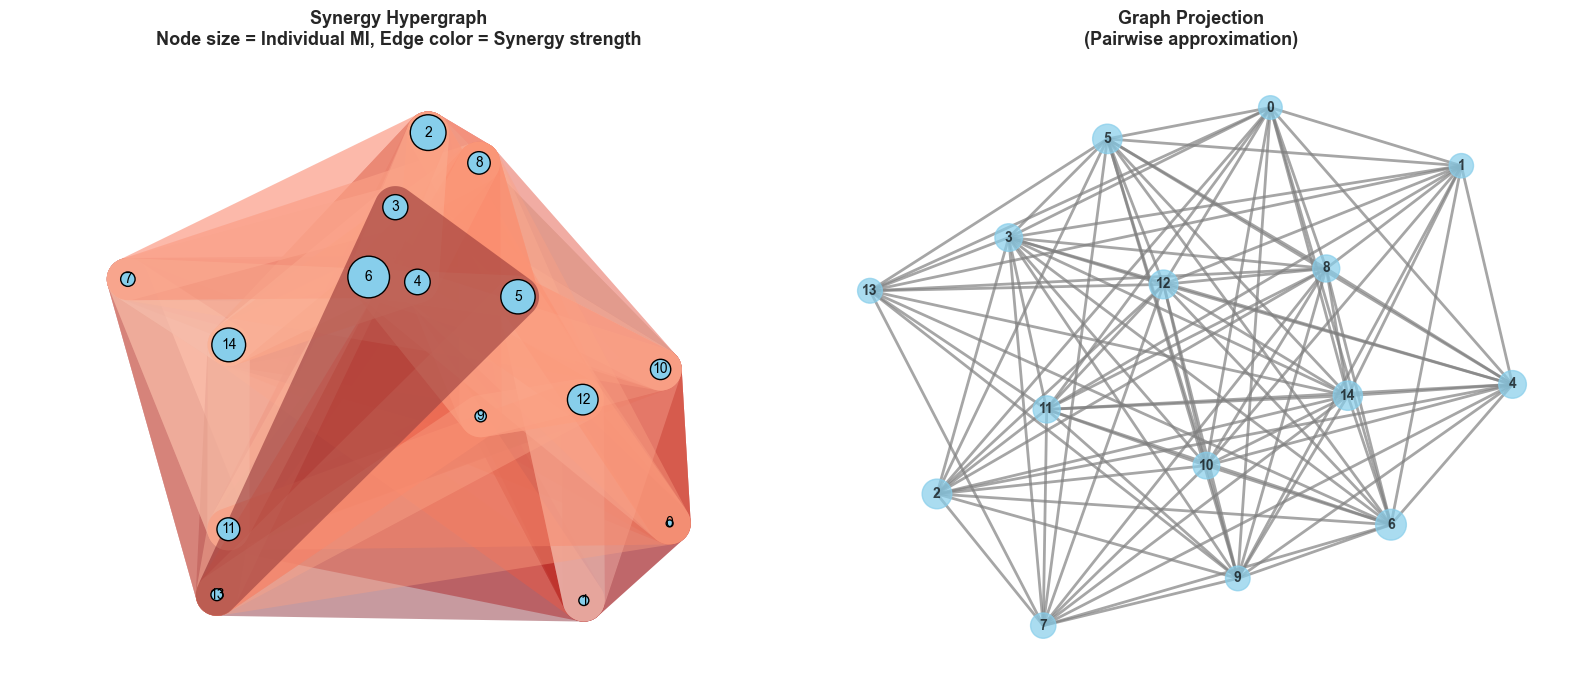
\includegraphics[keepaspectratio]{05_xgi_hypergraph_networks_files/figure-pdf/cell-8-output-1.png}}

\begin{verbatim}

🎨 Visualization Interpretation:
============================================================
Left (Hypergraph):
  • Colored hulls show which neurons interact together
  • Larger nodes = stronger individual information
  • Darker edges = stronger synergy

Right (Graph):
  • Loses information about which neurons form groups
  • Can't distinguish {1,2,3} triplet from separate {1,2}, {2,3}, {1,3} pairs

✨ Hypergraph representation preserves the discovered structure!
\end{verbatim}

\section{Part 3: Hypergraph Statistics and Network
Analysis}\label{part-3-hypergraph-statistics-and-network-analysis}

\subsection{Node-Level Statistics}\label{node-level-statistics}

XGI provides many built-in statistics for analyzing hypergraph
structure. The most important is \textbf{node degree} - how many
hyperedges include each node?

For our synergy network: - \textbf{High degree}: Neuron participates in
many synergistic ensembles - \textbf{Low degree}: Neuron works mostly
independently - \textbf{Zero degree}: Neuron doesn't participate in any
detected synergies

Let's analyze the network:

\begin{Shaded}
\begin{Highlighting}[]
\CommentTok{\# Compute node statistics}
\BuiltInTok{print}\NormalTok{(}\StringTok{"Node Statistics in Synergy Hypergraph"}\NormalTok{)}
\BuiltInTok{print}\NormalTok{(}\StringTok{"="} \OperatorTok{*} \DecValTok{60}\NormalTok{)}

\CommentTok{\# Degree: how many hyperedges contain each node}
\NormalTok{degrees }\OperatorTok{=}\NormalTok{ H\_synergy.degree()}

\CommentTok{\# Create DataFrame for analysis}
\NormalTok{node\_stats }\OperatorTok{=}\NormalTok{ pd.DataFrame(\{}
    \StringTok{\textquotesingle{}Neuron\textquotesingle{}}\NormalTok{: }\BuiltInTok{range}\NormalTok{(H\_synergy.num\_nodes),}
    \StringTok{\textquotesingle{}Degree\textquotesingle{}}\NormalTok{: [degrees.get(n, }\DecValTok{0}\NormalTok{) }\ControlFlowTok{for}\NormalTok{ n }\KeywordTok{in} \BuiltInTok{range}\NormalTok{(H\_synergy.num\_nodes)],}
    \StringTok{\textquotesingle{}Individual\_MI\textquotesingle{}}\NormalTok{: [neuron\_mi.get(n, }\DecValTok{0}\NormalTok{) }\ControlFlowTok{for}\NormalTok{ n }\KeywordTok{in} \BuiltInTok{range}\NormalTok{(H\_synergy.num\_nodes)]}
\NormalTok{\})}

\CommentTok{\# Sort by degree}
\NormalTok{node\_stats }\OperatorTok{=}\NormalTok{ node\_stats.sort\_values(}\StringTok{\textquotesingle{}Degree\textquotesingle{}}\NormalTok{, ascending}\OperatorTok{=}\VariableTok{False}\NormalTok{)}

\BuiltInTok{print}\NormalTok{(}\StringTok{"}\CharTok{\textbackslash{}n}\StringTok{Top 5 neurons by synergy participation:"}\NormalTok{)}
\BuiltInTok{print}\NormalTok{(node\_stats.head(}\DecValTok{5}\NormalTok{).to\_string(index}\OperatorTok{=}\VariableTok{False}\NormalTok{))}

\BuiltInTok{print}\NormalTok{(}\StringTok{"}\CharTok{\textbackslash{}n}\StringTok{Bottom 5 neurons:"}\NormalTok{)}
\BuiltInTok{print}\NormalTok{(node\_stats.tail(}\DecValTok{5}\NormalTok{).to\_string(index}\OperatorTok{=}\VariableTok{False}\NormalTok{))}

\CommentTok{\# Correlation between degree and individual MI}
\NormalTok{correlation }\OperatorTok{=}\NormalTok{ node\_stats[}\StringTok{\textquotesingle{}Degree\textquotesingle{}}\NormalTok{].corr(node\_stats[}\StringTok{\textquotesingle{}Individual\_MI\textquotesingle{}}\NormalTok{])}
\BuiltInTok{print}\NormalTok{(}\SpecialStringTok{f"}\CharTok{\textbackslash{}n}\SpecialStringTok{Correlation (Degree vs Individual MI): }\SpecialCharTok{\{}\NormalTok{correlation}\SpecialCharTok{:.3f\}}\SpecialStringTok{"}\NormalTok{)}

\ControlFlowTok{if}\NormalTok{ correlation }\OperatorTok{\textgreater{}} \FloatTok{0.5}\NormalTok{:}
    \BuiltInTok{print}\NormalTok{(}\StringTok{"  ✓ Strong positive correlation"}\NormalTok{)}
    \BuiltInTok{print}\NormalTok{(}\StringTok{"  → Neurons with high individual MI also participate in synergies"}\NormalTok{)}
\ControlFlowTok{elif}\NormalTok{ correlation }\OperatorTok{\textless{}} \OperatorTok{{-}}\FloatTok{0.5}\NormalTok{:}
    \BuiltInTok{print}\NormalTok{(}\StringTok{"  ⚠️  Strong negative correlation"}\NormalTok{)}
    \BuiltInTok{print}\NormalTok{(}\StringTok{"  → Neurons work EITHER individually OR synergistically (not both)"}\NormalTok{)}
\ControlFlowTok{else}\NormalTok{:}
    \BuiltInTok{print}\NormalTok{(}\StringTok{"  → Weak correlation"}\NormalTok{)}
    \BuiltInTok{print}\NormalTok{(}\StringTok{"  → Individual and synergistic coding are independent"}\NormalTok{)}

\CommentTok{\# Visualize relationship}
\NormalTok{fig, (ax1, ax2, ax3) }\OperatorTok{=}\NormalTok{ plt.subplots(}\DecValTok{1}\NormalTok{, }\DecValTok{3}\NormalTok{, figsize}\OperatorTok{=}\NormalTok{(}\DecValTok{18}\NormalTok{, }\DecValTok{5}\NormalTok{))}

\CommentTok{\# Panel 1: Degree distribution}
\NormalTok{ax1.hist(node\_stats[}\StringTok{\textquotesingle{}Degree\textquotesingle{}}\NormalTok{], bins}\OperatorTok{=}\BuiltInTok{range}\NormalTok{(node\_stats[}\StringTok{\textquotesingle{}Degree\textquotesingle{}}\NormalTok{].}\BuiltInTok{max}\NormalTok{()}\OperatorTok{+}\DecValTok{2}\NormalTok{),}
\NormalTok{         color}\OperatorTok{=}\StringTok{\textquotesingle{}\#457B9D\textquotesingle{}}\NormalTok{, alpha}\OperatorTok{=}\FloatTok{0.7}\NormalTok{, edgecolor}\OperatorTok{=}\StringTok{\textquotesingle{}black\textquotesingle{}}\NormalTok{, linewidth}\OperatorTok{=}\FloatTok{1.5}\NormalTok{)}
\NormalTok{ax1.set\_xlabel(}\StringTok{\textquotesingle{}Degree (\# synergistic triplets)\textquotesingle{}}\NormalTok{, fontsize}\OperatorTok{=}\DecValTok{11}\NormalTok{, fontweight}\OperatorTok{=}\StringTok{\textquotesingle{}bold\textquotesingle{}}\NormalTok{)}
\NormalTok{ax1.set\_ylabel(}\StringTok{\textquotesingle{}Number of Neurons\textquotesingle{}}\NormalTok{, fontsize}\OperatorTok{=}\DecValTok{11}\NormalTok{, fontweight}\OperatorTok{=}\StringTok{\textquotesingle{}bold\textquotesingle{}}\NormalTok{)}
\NormalTok{ax1.set\_title(}\StringTok{\textquotesingle{}Distribution of Synergy Participation\textquotesingle{}}\NormalTok{, fontsize}\OperatorTok{=}\DecValTok{12}\NormalTok{, fontweight}\OperatorTok{=}\StringTok{\textquotesingle{}bold\textquotesingle{}}\NormalTok{)}
\NormalTok{ax1.grid(}\VariableTok{True}\NormalTok{, alpha}\OperatorTok{=}\FloatTok{0.3}\NormalTok{, axis}\OperatorTok{=}\StringTok{\textquotesingle{}y\textquotesingle{}}\NormalTok{)}

\CommentTok{\# Panel 2: Individual MI distribution  }
\NormalTok{ax2.hist(node\_stats[}\StringTok{\textquotesingle{}Individual\_MI\textquotesingle{}}\NormalTok{], bins}\OperatorTok{=}\DecValTok{15}\NormalTok{, color}\OperatorTok{=}\StringTok{\textquotesingle{}\#E63946\textquotesingle{}}\NormalTok{, }
\NormalTok{         alpha}\OperatorTok{=}\FloatTok{0.7}\NormalTok{, edgecolor}\OperatorTok{=}\StringTok{\textquotesingle{}black\textquotesingle{}}\NormalTok{, linewidth}\OperatorTok{=}\FloatTok{1.5}\NormalTok{)}
\NormalTok{ax2.set\_xlabel(}\StringTok{\textquotesingle{}Individual MI (bits)\textquotesingle{}}\NormalTok{, fontsize}\OperatorTok{=}\DecValTok{11}\NormalTok{, fontweight}\OperatorTok{=}\StringTok{\textquotesingle{}bold\textquotesingle{}}\NormalTok{)}
\NormalTok{ax2.set\_ylabel(}\StringTok{\textquotesingle{}Number of Neurons\textquotesingle{}}\NormalTok{, fontsize}\OperatorTok{=}\DecValTok{11}\NormalTok{, fontweight}\OperatorTok{=}\StringTok{\textquotesingle{}bold\textquotesingle{}}\NormalTok{)}
\NormalTok{ax2.set\_title(}\StringTok{\textquotesingle{}Distribution of Individual Information\textquotesingle{}}\NormalTok{, fontsize}\OperatorTok{=}\DecValTok{12}\NormalTok{, fontweight}\OperatorTok{=}\StringTok{\textquotesingle{}bold\textquotesingle{}}\NormalTok{)}
\NormalTok{ax2.grid(}\VariableTok{True}\NormalTok{, alpha}\OperatorTok{=}\FloatTok{0.3}\NormalTok{, axis}\OperatorTok{=}\StringTok{\textquotesingle{}y\textquotesingle{}}\NormalTok{)}

\CommentTok{\# Panel 3: Scatter plot}
\NormalTok{ax3.scatter(node\_stats[}\StringTok{\textquotesingle{}Degree\textquotesingle{}}\NormalTok{], node\_stats[}\StringTok{\textquotesingle{}Individual\_MI\textquotesingle{}}\NormalTok{], }
\NormalTok{            s}\OperatorTok{=}\DecValTok{100}\NormalTok{, alpha}\OperatorTok{=}\FloatTok{0.6}\NormalTok{, color}\OperatorTok{=}\StringTok{\textquotesingle{}\#A8DADC\textquotesingle{}}\NormalTok{, edgecolor}\OperatorTok{=}\StringTok{\textquotesingle{}black\textquotesingle{}}\NormalTok{, linewidth}\OperatorTok{=}\FloatTok{1.5}\NormalTok{)}

\CommentTok{\# Add regression line}
\NormalTok{z }\OperatorTok{=}\NormalTok{ np.polyfit(node\_stats[}\StringTok{\textquotesingle{}Degree\textquotesingle{}}\NormalTok{], node\_stats[}\StringTok{\textquotesingle{}Individual\_MI\textquotesingle{}}\NormalTok{], }\DecValTok{1}\NormalTok{)}
\NormalTok{p }\OperatorTok{=}\NormalTok{ np.poly1d(z)}
\NormalTok{degree\_range }\OperatorTok{=}\NormalTok{ np.linspace(node\_stats[}\StringTok{\textquotesingle{}Degree\textquotesingle{}}\NormalTok{].}\BuiltInTok{min}\NormalTok{(), node\_stats[}\StringTok{\textquotesingle{}Degree\textquotesingle{}}\NormalTok{].}\BuiltInTok{max}\NormalTok{(), }\DecValTok{100}\NormalTok{)}
\NormalTok{ax3.plot(degree\_range, p(degree\_range), }\StringTok{"r{-}{-}"}\NormalTok{, linewidth}\OperatorTok{=}\DecValTok{2}\NormalTok{, alpha}\OperatorTok{=}\FloatTok{0.8}\NormalTok{,}
\NormalTok{         label}\OperatorTok{=}\SpecialStringTok{f\textquotesingle{}r = }\SpecialCharTok{\{}\NormalTok{correlation}\SpecialCharTok{:.3f\}}\SpecialStringTok{\textquotesingle{}}\NormalTok{)}

\CommentTok{\# Label interesting neurons}
\ControlFlowTok{for}\NormalTok{ idx, row }\KeywordTok{in}\NormalTok{ node\_stats.head(}\DecValTok{3}\NormalTok{).iterrows():}
\NormalTok{    ax3.annotate(}\SpecialStringTok{f"N}\SpecialCharTok{\{}\NormalTok{row[}\StringTok{\textquotesingle{}Neuron\textquotesingle{}}\NormalTok{]}\SpecialCharTok{\}}\SpecialStringTok{"}\NormalTok{, }
\NormalTok{                xy}\OperatorTok{=}\NormalTok{(row[}\StringTok{\textquotesingle{}Degree\textquotesingle{}}\NormalTok{], row[}\StringTok{\textquotesingle{}Individual\_MI\textquotesingle{}}\NormalTok{]),}
\NormalTok{                xytext}\OperatorTok{=}\NormalTok{(}\DecValTok{5}\NormalTok{, }\DecValTok{5}\NormalTok{), textcoords}\OperatorTok{=}\StringTok{\textquotesingle{}offset points\textquotesingle{}}\NormalTok{,}
\NormalTok{                fontsize}\OperatorTok{=}\DecValTok{9}\NormalTok{, fontweight}\OperatorTok{=}\StringTok{\textquotesingle{}bold\textquotesingle{}}\NormalTok{,}
\NormalTok{                bbox}\OperatorTok{=}\BuiltInTok{dict}\NormalTok{(boxstyle}\OperatorTok{=}\StringTok{\textquotesingle{}round\textquotesingle{}}\NormalTok{, facecolor}\OperatorTok{=}\StringTok{\textquotesingle{}yellow\textquotesingle{}}\NormalTok{, alpha}\OperatorTok{=}\FloatTok{0.7}\NormalTok{))}

\NormalTok{ax3.set\_xlabel(}\StringTok{\textquotesingle{}Degree (synergy participation)\textquotesingle{}}\NormalTok{, fontsize}\OperatorTok{=}\DecValTok{11}\NormalTok{, fontweight}\OperatorTok{=}\StringTok{\textquotesingle{}bold\textquotesingle{}}\NormalTok{)}
\NormalTok{ax3.set\_ylabel(}\StringTok{\textquotesingle{}Individual MI (bits)\textquotesingle{}}\NormalTok{, fontsize}\OperatorTok{=}\DecValTok{11}\NormalTok{, fontweight}\OperatorTok{=}\StringTok{\textquotesingle{}bold\textquotesingle{}}\NormalTok{)}
\NormalTok{ax3.set\_title(}\StringTok{\textquotesingle{}Individual vs Synergistic Coding\textquotesingle{}}\NormalTok{, fontsize}\OperatorTok{=}\DecValTok{12}\NormalTok{, fontweight}\OperatorTok{=}\StringTok{\textquotesingle{}bold\textquotesingle{}}\NormalTok{)}
\NormalTok{ax3.legend(fontsize}\OperatorTok{=}\DecValTok{11}\NormalTok{)}
\NormalTok{ax3.grid(}\VariableTok{True}\NormalTok{, alpha}\OperatorTok{=}\FloatTok{0.3}\NormalTok{)}

\NormalTok{plt.tight\_layout()}
\NormalTok{plt.show()}

\BuiltInTok{print}\NormalTok{(}\StringTok{"}\CharTok{\textbackslash{}n}\StringTok{💡 Network Analysis Insights:"}\NormalTok{)}
\BuiltInTok{print}\NormalTok{(}\StringTok{"="} \OperatorTok{*} \DecValTok{60}\NormalTok{)}
\BuiltInTok{print}\NormalTok{(}\SpecialStringTok{f"• }\SpecialCharTok{\{}\BuiltInTok{len}\NormalTok{([d }\ControlFlowTok{for}\NormalTok{ d }\KeywordTok{in}\NormalTok{ degrees.values() }\ControlFlowTok{if}\NormalTok{ d }\OperatorTok{\textgreater{}=} \DecValTok{5}\NormalTok{])}\SpecialCharTok{\}}\SpecialStringTok{ neurons are \textquotesingle{}hubs\textquotesingle{} (degree ≥ 5)"}\NormalTok{)}
\BuiltInTok{print}\NormalTok{(}\SpecialStringTok{f"• These participate in many synergistic ensembles"}\NormalTok{)}
\BuiltInTok{print}\NormalTok{(}\SpecialStringTok{f"• Hub neurons might be critical for population coding"}\NormalTok{)}
\BuiltInTok{print}\NormalTok{(}\SpecialStringTok{f"• Removing them could disproportionately impact information"}\NormalTok{)}
\end{Highlighting}
\end{Shaded}

\begin{verbatim}
Node Statistics in Synergy Hypergraph
============================================================

Top 5 neurons by synergy participation:
 Neuron  Degree  Individual_MI
      6      21       1.636460
     12      21       1.422575
      5      19       1.494134
      2      18       1.521210
      4      18       1.324523

Bottom 5 neurons:
 Neuron  Degree  Individual_MI
      9      14       1.048754
     11      14       1.272447
      1      12       1.022916
      0      11       0.963949
     13      11       1.060065

Correlation (Degree vs Individual MI): 0.908
  ✓ Strong positive correlation
  → Neurons with high individual MI also participate in synergies
\end{verbatim}

\pandocbounded{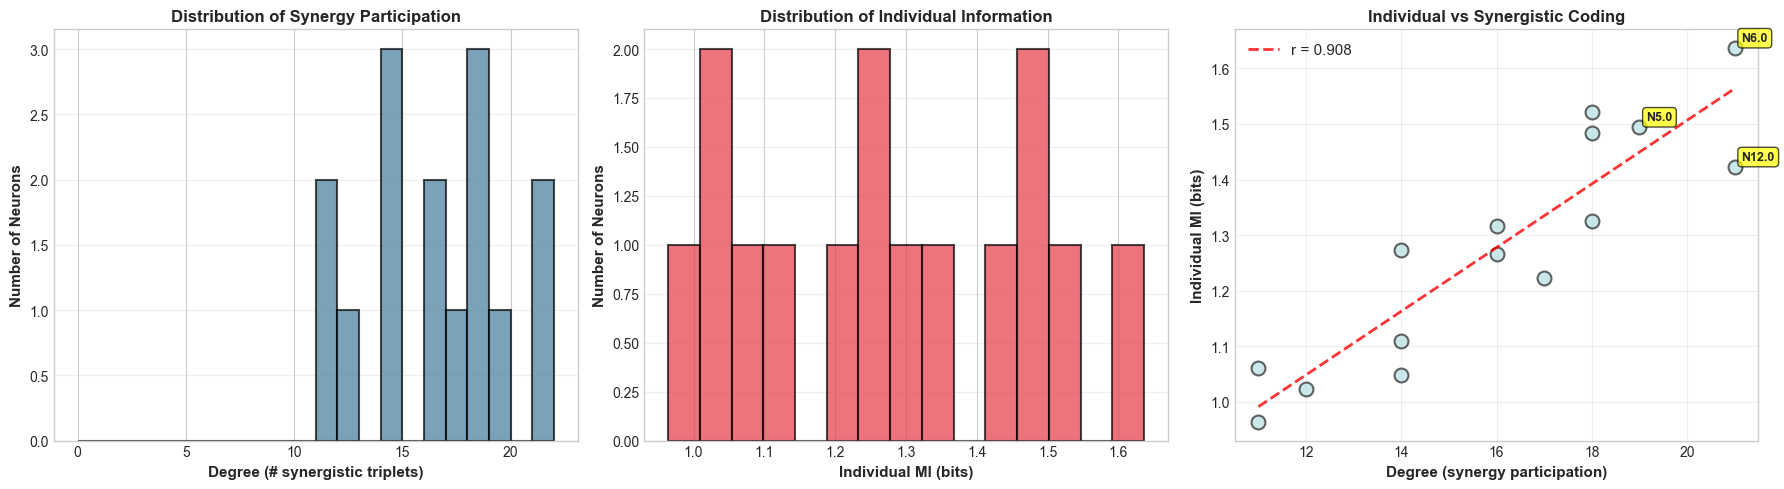
\includegraphics[keepaspectratio]{05_xgi_hypergraph_networks_files/figure-pdf/cell-9-output-2.png}}

\begin{verbatim}

💡 Network Analysis Insights:
============================================================
• 15 neurons are 'hubs' (degree ≥ 5)
• These participate in many synergistic ensembles
• Hub neurons might be critical for population coding
• Removing them could disproportionately impact information
\end{verbatim}

\subsection{Edge-Level Statistics}\label{edge-level-statistics}

We can also analyze the hyperedges themselves. Each hyperedge represents
a synergistic ensemble, and we stored the O-information strength as an
edge attribute:

\begin{Shaded}
\begin{Highlighting}[]
\CommentTok{\# Analyze hyperedges}
\BuiltInTok{print}\NormalTok{(}\StringTok{"Hyperedge Statistics"}\NormalTok{)}
\BuiltInTok{print}\NormalTok{(}\StringTok{"="} \OperatorTok{*} \DecValTok{60}\NormalTok{)}

\CommentTok{\# Get edge properties}
\NormalTok{edge\_data }\OperatorTok{=}\NormalTok{ []}
\ControlFlowTok{for}\NormalTok{ edge\_id }\KeywordTok{in}\NormalTok{ H\_synergy.edges:}
\NormalTok{    members }\OperatorTok{=}\NormalTok{ H\_synergy.edges.members(edge\_id)}
\NormalTok{    oinfo }\OperatorTok{=}\NormalTok{ H\_synergy.edges[edge\_id][}\StringTok{\textquotesingle{}oinfo\textquotesingle{}}\NormalTok{]}
\NormalTok{    weight }\OperatorTok{=}\NormalTok{ H\_synergy.edges[edge\_id][}\StringTok{\textquotesingle{}weight\textquotesingle{}}\NormalTok{]}
    
    \CommentTok{\# Average individual MI of members}
\NormalTok{    avg\_individual\_mi }\OperatorTok{=}\NormalTok{ np.mean([neuron\_mi[n] }\ControlFlowTok{for}\NormalTok{ n }\KeywordTok{in}\NormalTok{ members])}
    
\NormalTok{    edge\_data.append(\{}
        \StringTok{\textquotesingle{}Edge\_ID\textquotesingle{}}\NormalTok{: edge\_id,}
        \StringTok{\textquotesingle{}Members\textquotesingle{}}\NormalTok{: members,}
        \StringTok{\textquotesingle{}Size\textquotesingle{}}\NormalTok{: }\BuiltInTok{len}\NormalTok{(members),}
        \StringTok{\textquotesingle{}O{-}info\textquotesingle{}}\NormalTok{: oinfo,}
        \StringTok{\textquotesingle{}Strength\textquotesingle{}}\NormalTok{: weight,}
        \StringTok{\textquotesingle{}Avg\_Individual\_MI\textquotesingle{}}\NormalTok{: avg\_individual\_mi}
\NormalTok{    \})}

\NormalTok{edge\_df }\OperatorTok{=}\NormalTok{ pd.DataFrame(edge\_data)}
\NormalTok{edge\_df }\OperatorTok{=}\NormalTok{ edge\_df.sort\_values(}\StringTok{\textquotesingle{}Strength\textquotesingle{}}\NormalTok{, ascending}\OperatorTok{=}\VariableTok{False}\NormalTok{)}

\BuiltInTok{print}\NormalTok{(}\StringTok{"}\CharTok{\textbackslash{}n}\StringTok{Top 5 strongest synergistic ensembles:"}\NormalTok{)}
\ControlFlowTok{for}\NormalTok{ idx, row }\KeywordTok{in}\NormalTok{ edge\_df.head(}\DecValTok{5}\NormalTok{).iterrows():}
    \BuiltInTok{print}\NormalTok{(}\SpecialStringTok{f"}\CharTok{\textbackslash{}n}\SpecialStringTok{Edge }\SpecialCharTok{\{}\NormalTok{row[}\StringTok{\textquotesingle{}Edge\_ID\textquotesingle{}}\NormalTok{]}\SpecialCharTok{\}}\SpecialStringTok{: Neurons }\SpecialCharTok{\{}\BuiltInTok{list}\NormalTok{(row[}\StringTok{\textquotesingle{}Members\textquotesingle{}}\NormalTok{])}\SpecialCharTok{\}}\SpecialStringTok{"}\NormalTok{)}
    \BuiltInTok{print}\NormalTok{(}\SpecialStringTok{f"  O{-}info: }\SpecialCharTok{\{}\NormalTok{row[}\StringTok{\textquotesingle{}O{-}info\textquotesingle{}}\NormalTok{]}\SpecialCharTok{:.4f\}}\SpecialStringTok{ bits (synergy strength)"}\NormalTok{)}
    \BuiltInTok{print}\NormalTok{(}\SpecialStringTok{f"  Avg individual MI: }\SpecialCharTok{\{}\NormalTok{row[}\StringTok{\textquotesingle{}Avg\_Individual\_MI\textquotesingle{}}\NormalTok{]}\SpecialCharTok{:.4f\}}\SpecialStringTok{ bits"}\NormalTok{)}

\CommentTok{\# Visualize edge properties}
\NormalTok{fig, (ax1, ax2) }\OperatorTok{=}\NormalTok{ plt.subplots(}\DecValTok{1}\NormalTok{, }\DecValTok{2}\NormalTok{, figsize}\OperatorTok{=}\NormalTok{(}\DecValTok{14}\NormalTok{, }\DecValTok{5}\NormalTok{))}

\CommentTok{\# Distribution of synergy strengths}
\NormalTok{ax1.hist(edge\_df[}\StringTok{\textquotesingle{}Strength\textquotesingle{}}\NormalTok{], bins}\OperatorTok{=}\DecValTok{15}\NormalTok{, color}\OperatorTok{=}\StringTok{\textquotesingle{}\#E63946\textquotesingle{}}\NormalTok{, }
\NormalTok{         alpha}\OperatorTok{=}\FloatTok{0.7}\NormalTok{, edgecolor}\OperatorTok{=}\StringTok{\textquotesingle{}black\textquotesingle{}}\NormalTok{, linewidth}\OperatorTok{=}\FloatTok{1.5}\NormalTok{)}
\NormalTok{ax1.axvline(edge\_df[}\StringTok{\textquotesingle{}Strength\textquotesingle{}}\NormalTok{].mean(), color}\OperatorTok{=}\StringTok{\textquotesingle{}blue\textquotesingle{}}\NormalTok{, linestyle}\OperatorTok{=}\StringTok{\textquotesingle{}{-}{-}\textquotesingle{}}\NormalTok{, }
\NormalTok{            linewidth}\OperatorTok{=}\DecValTok{2}\NormalTok{, label}\OperatorTok{=}\SpecialStringTok{f"Mean = }\SpecialCharTok{\{}\NormalTok{edge\_df[}\StringTok{\textquotesingle{}Strength\textquotesingle{}}\NormalTok{]}\SpecialCharTok{.}\NormalTok{mean()}\SpecialCharTok{:.3f\}}\SpecialStringTok{"}\NormalTok{)}
\NormalTok{ax1.set\_xlabel(}\StringTok{\textquotesingle{}Synergy Strength (|O{-}info|, bits)\textquotesingle{}}\NormalTok{, fontsize}\OperatorTok{=}\DecValTok{11}\NormalTok{, fontweight}\OperatorTok{=}\StringTok{\textquotesingle{}bold\textquotesingle{}}\NormalTok{)}
\NormalTok{ax1.set\_ylabel(}\StringTok{\textquotesingle{}Count\textquotesingle{}}\NormalTok{, fontsize}\OperatorTok{=}\DecValTok{11}\NormalTok{, fontweight}\OperatorTok{=}\StringTok{\textquotesingle{}bold\textquotesingle{}}\NormalTok{)}
\NormalTok{ax1.set\_title(}\StringTok{\textquotesingle{}Distribution of Synergy Strengths\textquotesingle{}}\NormalTok{, fontsize}\OperatorTok{=}\DecValTok{12}\NormalTok{, fontweight}\OperatorTok{=}\StringTok{\textquotesingle{}bold\textquotesingle{}}\NormalTok{)}
\NormalTok{ax1.legend(fontsize}\OperatorTok{=}\DecValTok{10}\NormalTok{)}
\NormalTok{ax1.grid(}\VariableTok{True}\NormalTok{, alpha}\OperatorTok{=}\FloatTok{0.3}\NormalTok{, axis}\OperatorTok{=}\StringTok{\textquotesingle{}y\textquotesingle{}}\NormalTok{)}

\CommentTok{\# Relationship: synergy strength vs average individual MI}
\NormalTok{ax2.scatter(edge\_df[}\StringTok{\textquotesingle{}Avg\_Individual\_MI\textquotesingle{}}\NormalTok{], edge\_df[}\StringTok{\textquotesingle{}Strength\textquotesingle{}}\NormalTok{],}
\NormalTok{            s}\OperatorTok{=}\DecValTok{100}\NormalTok{, alpha}\OperatorTok{=}\FloatTok{0.6}\NormalTok{, color}\OperatorTok{=}\StringTok{\textquotesingle{}\#457B9D\textquotesingle{}}\NormalTok{, edgecolor}\OperatorTok{=}\StringTok{\textquotesingle{}black\textquotesingle{}}\NormalTok{, linewidth}\OperatorTok{=}\FloatTok{1.5}\NormalTok{)}
\NormalTok{ax2.set\_xlabel(}\StringTok{\textquotesingle{}Average Individual MI of Members (bits)\textquotesingle{}}\NormalTok{, fontsize}\OperatorTok{=}\DecValTok{11}\NormalTok{, fontweight}\OperatorTok{=}\StringTok{\textquotesingle{}bold\textquotesingle{}}\NormalTok{)}
\NormalTok{ax2.set\_ylabel(}\StringTok{\textquotesingle{}Synergy Strength (bits)\textquotesingle{}}\NormalTok{, fontsize}\OperatorTok{=}\DecValTok{11}\NormalTok{, fontweight}\OperatorTok{=}\StringTok{\textquotesingle{}bold\textquotesingle{}}\NormalTok{)}
\NormalTok{ax2.set\_title(}\StringTok{\textquotesingle{}Synergy vs Individual Information\textquotesingle{}}\NormalTok{, fontsize}\OperatorTok{=}\DecValTok{12}\NormalTok{, fontweight}\OperatorTok{=}\StringTok{\textquotesingle{}bold\textquotesingle{}}\NormalTok{)}
\NormalTok{ax2.grid(}\VariableTok{True}\NormalTok{, alpha}\OperatorTok{=}\FloatTok{0.3}\NormalTok{)}

\CommentTok{\# Correlation}
\NormalTok{corr\_edge }\OperatorTok{=}\NormalTok{ edge\_df[}\StringTok{\textquotesingle{}Avg\_Individual\_MI\textquotesingle{}}\NormalTok{].corr(edge\_df[}\StringTok{\textquotesingle{}Strength\textquotesingle{}}\NormalTok{])}
\NormalTok{ax2.text(}\FloatTok{0.05}\NormalTok{, }\FloatTok{0.95}\NormalTok{, }\SpecialStringTok{f\textquotesingle{}Correlation: }\SpecialCharTok{\{}\NormalTok{corr\_edge}\SpecialCharTok{:.3f\}}\SpecialStringTok{\textquotesingle{}}\NormalTok{, }
\NormalTok{         transform}\OperatorTok{=}\NormalTok{ax2.transAxes, fontsize}\OperatorTok{=}\DecValTok{11}\NormalTok{, fontweight}\OperatorTok{=}\StringTok{\textquotesingle{}bold\textquotesingle{}}\NormalTok{,}
\NormalTok{         bbox}\OperatorTok{=}\BuiltInTok{dict}\NormalTok{(boxstyle}\OperatorTok{=}\StringTok{\textquotesingle{}round\textquotesingle{}}\NormalTok{, facecolor}\OperatorTok{=}\StringTok{\textquotesingle{}wheat\textquotesingle{}}\NormalTok{, alpha}\OperatorTok{=}\FloatTok{0.8}\NormalTok{),}
\NormalTok{         verticalalignment}\OperatorTok{=}\StringTok{\textquotesingle{}top\textquotesingle{}}\NormalTok{)}

\NormalTok{plt.tight\_layout()}
\NormalTok{plt.show()}

\BuiltInTok{print}\NormalTok{(}\StringTok{"}\CharTok{\textbackslash{}n}\StringTok{🎯 Interpretation:"}\NormalTok{)}
\ControlFlowTok{if}\NormalTok{ corr\_edge }\OperatorTok{\textgreater{}} \FloatTok{0.3}\NormalTok{:}
    \BuiltInTok{print}\NormalTok{(}\StringTok{"   Ensembles with stronger individual coding also show more synergy"}\NormalTok{)}
    \BuiltInTok{print}\NormalTok{(}\StringTok{"   → Synergy ENHANCES already informative neurons"}\NormalTok{)}
\ControlFlowTok{else}\NormalTok{:}
    \BuiltInTok{print}\NormalTok{(}\StringTok{"   Synergy is independent of individual coding strength"}\NormalTok{)}
    \BuiltInTok{print}\NormalTok{(}\StringTok{"   → Different coding strategies operate independently"}\NormalTok{)}
\end{Highlighting}
\end{Shaded}

\begin{verbatim}
Hyperedge Statistics
============================================================

Top 5 strongest synergistic ensembles:

Edge 0: Neurons [5, 3, 13]
  O-info: -0.5987 bits (synergy strength)
  Avg individual MI: 1.2900 bits

Edge 1: Neurons [0, 2, 10]
  O-info: -0.5948 bits (synergy strength)
  Avg individual MI: 1.2359 bits

Edge 2: Neurons [0, 1, 4]
  O-info: -0.5880 bits (synergy strength)
  Avg individual MI: 1.1038 bits

Edge 3: Neurons [1, 13, 6]
  O-info: -0.5880 bits (synergy strength)
  Avg individual MI: 1.2398 bits

Edge 4: Neurons [11, 13, 7]
  O-info: -0.5879 bits (synergy strength)
  Avg individual MI: 1.1472 bits
\end{verbatim}

\pandocbounded{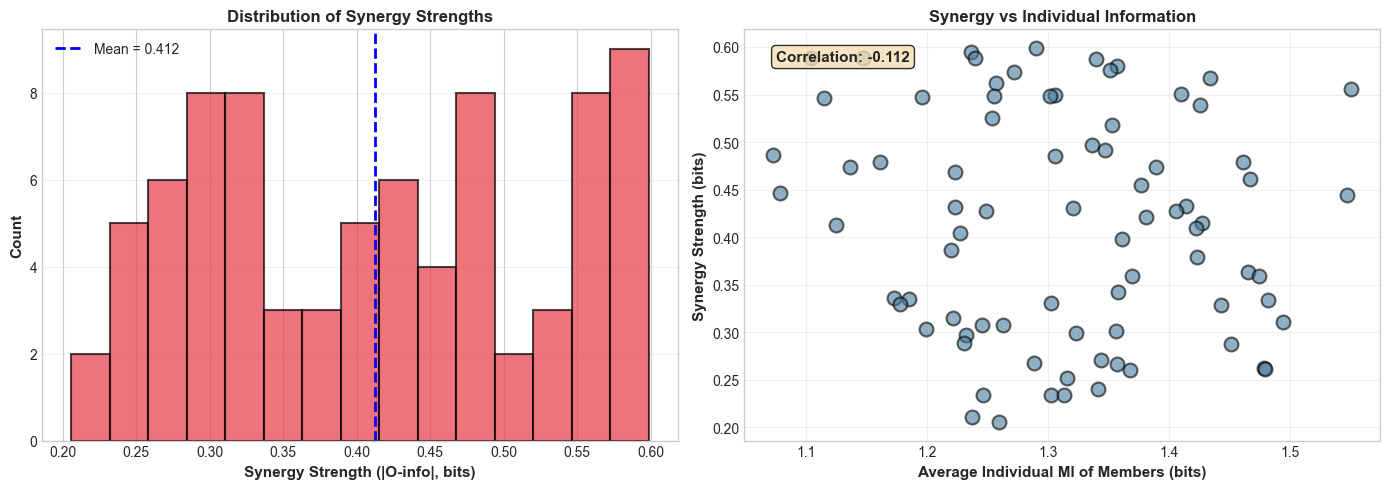
\includegraphics[keepaspectratio]{05_xgi_hypergraph_networks_files/figure-pdf/cell-10-output-2.png}}

\begin{verbatim}

🎯 Interpretation:
   Synergy is independent of individual coding strength
   → Different coding strategies operate independently
\end{verbatim}

\section{Part 4: Temporal Hypergraphs - Tracking Dynamic
Structure}\label{part-4-temporal-hypergraphs---tracking-dynamic-structure}

\subsection{From Static to Dynamic
Networks}\label{from-static-to-dynamic-networks}

In Notebook 4, we saw that information content changes over time. The
same is true for network structure! Connections that are strong during
stimulus processing might be weak during rest.

\textbf{Temporal hypergraphs} represent how network structure evolves.
We can: - Create a hypergraph snapshot for each time window - Track how
nodes' degrees change - Identify stable vs transient hyperedges - Detect
network reconfigurations

Let's simulate this by creating hypergraphs from dynamic connectivity
results:

\begin{Shaded}
\begin{Highlighting}[]
\KeywordTok{class}\NormalTok{ TemporalHypergraph:}
    \CommentTok{"""}
\CommentTok{    A sequence of hypergraphs over time.}
\CommentTok{    }
\CommentTok{    Useful for tracking how higher{-}order structure evolves.}
\CommentTok{    """}
    \KeywordTok{def} \FunctionTok{\_\_init\_\_}\NormalTok{(}\VariableTok{self}\NormalTok{, n\_nodes):}
        \VariableTok{self}\NormalTok{.snapshots }\OperatorTok{=}\NormalTok{ []  }\CommentTok{\# List of Hypergraph objects}
        \VariableTok{self}\NormalTok{.time\_points }\OperatorTok{=}\NormalTok{ []  }\CommentTok{\# Corresponding time labels}
        \VariableTok{self}\NormalTok{.n\_nodes }\OperatorTok{=}\NormalTok{ n\_nodes}
    
    \KeywordTok{def}\NormalTok{ add\_snapshot(}\VariableTok{self}\NormalTok{, hypergraph, time\_label):}
        \CommentTok{"""Add a hypergraph for a specific time point."""}
        \VariableTok{self}\NormalTok{.snapshots.append(hypergraph)}
        \VariableTok{self}\NormalTok{.time\_points.append(time\_label)}
    
    \KeywordTok{def}\NormalTok{ get\_node\_degree\_evolution(}\VariableTok{self}\NormalTok{, node\_id):}
        \CommentTok{"""Get degree of a node across all time points."""}
\NormalTok{        degrees }\OperatorTok{=}\NormalTok{ []}
        \ControlFlowTok{for}\NormalTok{ H }\KeywordTok{in} \VariableTok{self}\NormalTok{.snapshots:}
            \ControlFlowTok{if}\NormalTok{ node\_id }\KeywordTok{in}\NormalTok{ H.nodes:}
\NormalTok{                degrees.append(H.degree(node\_id))}
            \ControlFlowTok{else}\NormalTok{:}
\NormalTok{                degrees.append(}\DecValTok{0}\NormalTok{)}
        \ControlFlowTok{return}\NormalTok{ np.array(degrees)}
    
    \KeywordTok{def}\NormalTok{ get\_total\_edges\_evolution(}\VariableTok{self}\NormalTok{):}
        \CommentTok{"""Get number of hyperedges over time."""}
        \ControlFlowTok{return}\NormalTok{ np.array([H.num\_edges }\ControlFlowTok{for}\NormalTok{ H }\KeywordTok{in} \VariableTok{self}\NormalTok{.snapshots])}
    
    \KeywordTok{def}\NormalTok{ get\_persistent\_edges(}\VariableTok{self}\NormalTok{, min\_appearances}\OperatorTok{=}\DecValTok{3}\NormalTok{):}
        \CommentTok{"""Find hyperedges that appear in multiple snapshots."""}
        \ImportTok{from}\NormalTok{ collections }\ImportTok{import}\NormalTok{ Counter}
        
\NormalTok{        edge\_counts }\OperatorTok{=}\NormalTok{ Counter()}
        \ControlFlowTok{for}\NormalTok{ H }\KeywordTok{in} \VariableTok{self}\NormalTok{.snapshots:}
            \ControlFlowTok{for}\NormalTok{ members }\KeywordTok{in}\NormalTok{ H.edges.members():}
                \CommentTok{\# Convert to sorted tuple for hashing}
\NormalTok{                edge\_tuple }\OperatorTok{=} \BuiltInTok{tuple}\NormalTok{(}\BuiltInTok{sorted}\NormalTok{(members))}
\NormalTok{                edge\_counts[edge\_tuple] }\OperatorTok{+=} \DecValTok{1}
        
        \CommentTok{\# Return edges that appear \textgreater{}= min\_appearances times}
\NormalTok{        persistent }\OperatorTok{=}\NormalTok{ [(edge, count) }\ControlFlowTok{for}\NormalTok{ edge, count }\KeywordTok{in}\NormalTok{ edge\_counts.items() }
                     \ControlFlowTok{if}\NormalTok{ count }\OperatorTok{\textgreater{}=}\NormalTok{ min\_appearances]}
\NormalTok{        persistent.sort(key}\OperatorTok{=}\KeywordTok{lambda}\NormalTok{ x: x[}\DecValTok{1}\NormalTok{], reverse}\OperatorTok{=}\VariableTok{True}\NormalTok{)}
        
        \ControlFlowTok{return}\NormalTok{ persistent}

\BuiltInTok{print}\NormalTok{(}\StringTok{"TemporalHypergraph Class Defined ✓"}\NormalTok{)}
\BuiltInTok{print}\NormalTok{(}\StringTok{"}\CharTok{\textbackslash{}n}\StringTok{This will let us track network evolution over time"}\NormalTok{)}
\end{Highlighting}
\end{Shaded}

\begin{verbatim}
TemporalHypergraph Class Defined ✓

This will let us track network evolution over time
\end{verbatim}

\subsection{Simulating Time-Varying Synergistic
Structure}\label{simulating-time-varying-synergistic-structure}

Let's simulate a realistic scenario where synergistic ensembles change
during a task:

\begin{Shaded}
\begin{Highlighting}[]
\CommentTok{\# Simulate temporal evolution of synergistic structure}
\NormalTok{n\_neurons }\OperatorTok{=} \DecValTok{12}
\NormalTok{time\_windows }\OperatorTok{=}\NormalTok{ [}\StringTok{\textquotesingle{}Baseline}\CharTok{\textbackslash{}n}\StringTok{({-}200{-}0ms)\textquotesingle{}}\NormalTok{, }\StringTok{\textquotesingle{}Early}\CharTok{\textbackslash{}n}\StringTok{(0{-}200ms)\textquotesingle{}}\NormalTok{, }
                \StringTok{\textquotesingle{}Middle}\CharTok{\textbackslash{}n}\StringTok{(200{-}400ms)\textquotesingle{}}\NormalTok{, }\StringTok{\textquotesingle{}Late}\CharTok{\textbackslash{}n}\StringTok{(400{-}600ms)\textquotesingle{}}\NormalTok{, }\StringTok{\textquotesingle{}Post}\CharTok{\textbackslash{}n}\StringTok{(600{-}800ms)\textquotesingle{}}\NormalTok{]}
\NormalTok{n\_windows }\OperatorTok{=} \BuiltInTok{len}\NormalTok{(time\_windows)}

\CommentTok{\# Create temporal hypergraph}
\NormalTok{temporal\_hg }\OperatorTok{=}\NormalTok{ TemporalHypergraph(n\_nodes}\OperatorTok{=}\NormalTok{n\_neurons)}

\CommentTok{\# Simulate different network states}
\ControlFlowTok{for}\NormalTok{ w\_idx, window\_name }\KeywordTok{in} \BuiltInTok{enumerate}\NormalTok{(time\_windows):}
\NormalTok{    H\_window }\OperatorTok{=}\NormalTok{ xgi.Hypergraph()}
    
    \CommentTok{\# Add all nodes}
    \ControlFlowTok{for}\NormalTok{ n }\KeywordTok{in} \BuiltInTok{range}\NormalTok{(n\_neurons):}
\NormalTok{        H\_window.add\_node(n)}
    
    \CommentTok{\# Different connectivity patterns in each window}
    \ControlFlowTok{if}\NormalTok{ w\_idx }\OperatorTok{==} \DecValTok{0}\NormalTok{:  }\CommentTok{\# Baseline: sparse}
\NormalTok{        edges }\OperatorTok{=}\NormalTok{ [[}\DecValTok{0}\NormalTok{, }\DecValTok{1}\NormalTok{, }\DecValTok{2}\NormalTok{], [}\DecValTok{6}\NormalTok{, }\DecValTok{7}\NormalTok{, }\DecValTok{8}\NormalTok{]]}
    \ControlFlowTok{elif}\NormalTok{ w\_idx }\OperatorTok{==} \DecValTok{1}\NormalTok{:  }\CommentTok{\# Early: moderate}
\NormalTok{        edges }\OperatorTok{=}\NormalTok{ [[}\DecValTok{0}\NormalTok{, }\DecValTok{1}\NormalTok{, }\DecValTok{2}\NormalTok{], [}\DecValTok{3}\NormalTok{, }\DecValTok{4}\NormalTok{, }\DecValTok{5}\NormalTok{], [}\DecValTok{6}\NormalTok{, }\DecValTok{7}\NormalTok{, }\DecValTok{8}\NormalTok{]]}
    \ControlFlowTok{elif}\NormalTok{ w\_idx }\OperatorTok{==} \DecValTok{2}\NormalTok{:  }\CommentTok{\# Middle: rich (task period)}
\NormalTok{        edges }\OperatorTok{=}\NormalTok{ [[}\DecValTok{0}\NormalTok{, }\DecValTok{1}\NormalTok{, }\DecValTok{2}\NormalTok{], [}\DecValTok{1}\NormalTok{, }\DecValTok{2}\NormalTok{, }\DecValTok{3}\NormalTok{], [}\DecValTok{3}\NormalTok{, }\DecValTok{4}\NormalTok{, }\DecValTok{5}\NormalTok{], [}\DecValTok{4}\NormalTok{, }\DecValTok{5}\NormalTok{, }\DecValTok{6}\NormalTok{], }
\NormalTok{                [}\DecValTok{6}\NormalTok{, }\DecValTok{7}\NormalTok{, }\DecValTok{8}\NormalTok{], [}\DecValTok{7}\NormalTok{, }\DecValTok{8}\NormalTok{, }\DecValTok{9}\NormalTok{], [}\DecValTok{9}\NormalTok{, }\DecValTok{10}\NormalTok{, }\DecValTok{11}\NormalTok{]]}
    \ControlFlowTok{elif}\NormalTok{ w\_idx }\OperatorTok{==} \DecValTok{3}\NormalTok{:  }\CommentTok{\# Late: moderate  }
\NormalTok{        edges }\OperatorTok{=}\NormalTok{ [[}\DecValTok{1}\NormalTok{, }\DecValTok{2}\NormalTok{, }\DecValTok{3}\NormalTok{], [}\DecValTok{4}\NormalTok{, }\DecValTok{5}\NormalTok{, }\DecValTok{6}\NormalTok{], [}\DecValTok{7}\NormalTok{, }\DecValTok{8}\NormalTok{, }\DecValTok{9}\NormalTok{]]}
    \ControlFlowTok{else}\NormalTok{:  }\CommentTok{\# Post: returning to baseline}
\NormalTok{        edges }\OperatorTok{=}\NormalTok{ [[}\DecValTok{0}\NormalTok{, }\DecValTok{1}\NormalTok{, }\DecValTok{2}\NormalTok{], [}\DecValTok{6}\NormalTok{, }\DecValTok{7}\NormalTok{, }\DecValTok{8}\NormalTok{]]}
    
    \CommentTok{\# Add edges with random weights}
    \ControlFlowTok{for}\NormalTok{ edge }\KeywordTok{in}\NormalTok{ edges:}
\NormalTok{        weight }\OperatorTok{=} \FloatTok{0.2} \OperatorTok{+}\NormalTok{ np.random.rand() }\OperatorTok{*} \FloatTok{0.4}
\NormalTok{        H\_window.add\_edge(edge, weight}\OperatorTok{=}\NormalTok{weight)}
    
\NormalTok{    temporal\_hg.add\_snapshot(H\_window, window\_name)}

\BuiltInTok{print}\NormalTok{(}\StringTok{"Temporal Hypergraph Created"}\NormalTok{)}
\BuiltInTok{print}\NormalTok{(}\StringTok{"="} \OperatorTok{*} \DecValTok{60}\NormalTok{)}
\BuiltInTok{print}\NormalTok{(}\SpecialStringTok{f"Time windows: }\SpecialCharTok{\{}\NormalTok{n\_windows}\SpecialCharTok{\}}\SpecialStringTok{"}\NormalTok{)}
\BuiltInTok{print}\NormalTok{(}\SpecialStringTok{f"Neurons: }\SpecialCharTok{\{}\NormalTok{n\_neurons}\SpecialCharTok{\}}\SpecialStringTok{"}\NormalTok{)}

\CommentTok{\# Track network size over time}
\NormalTok{edge\_counts }\OperatorTok{=}\NormalTok{ temporal\_hg.get\_total\_edges\_evolution()}
\BuiltInTok{print}\NormalTok{(}\SpecialStringTok{f"}\CharTok{\textbackslash{}n}\SpecialStringTok{Hyperedges per window: }\SpecialCharTok{\{}\NormalTok{edge\_counts}\SpecialCharTok{\}}\SpecialStringTok{"}\NormalTok{)}
\BuiltInTok{print}\NormalTok{(}\SpecialStringTok{f"  Peak connectivity at window: }\SpecialCharTok{\{}\NormalTok{np}\SpecialCharTok{.}\NormalTok{argmax(edge\_counts)}\SpecialCharTok{\}}\SpecialStringTok{ (}\SpecialCharTok{\{}\NormalTok{time\_windows[np.argmax(edge\_counts)]}\SpecialCharTok{\}}\SpecialStringTok{)"}\NormalTok{)}

\CommentTok{\# Find persistent edges}
\NormalTok{persistent }\OperatorTok{=}\NormalTok{ temporal\_hg.get\_persistent\_edges(min\_appearances}\OperatorTok{=}\DecValTok{3}\NormalTok{)}
\BuiltInTok{print}\NormalTok{(}\SpecialStringTok{f"}\CharTok{\textbackslash{}n}\SpecialStringTok{Persistent hyperedges (appear in 3+ windows): }\SpecialCharTok{\{}\BuiltInTok{len}\NormalTok{(persistent)}\SpecialCharTok{\}}\SpecialStringTok{"}\NormalTok{)}
\ControlFlowTok{for}\NormalTok{ edge, count }\KeywordTok{in}\NormalTok{ persistent:}
    \BuiltInTok{print}\NormalTok{(}\SpecialStringTok{f"  Neurons }\SpecialCharTok{\{}\BuiltInTok{list}\NormalTok{(edge)}\SpecialCharTok{\}}\SpecialStringTok{: appears }\SpecialCharTok{\{}\NormalTok{count}\SpecialCharTok{\}}\SpecialStringTok{/}\SpecialCharTok{\{}\NormalTok{n\_windows}\SpecialCharTok{\}}\SpecialStringTok{ times"}\NormalTok{)}
\BuiltInTok{print}\NormalTok{(}\StringTok{"}\CharTok{\textbackslash{}n}\StringTok{✨ These represent stable functional ensembles!"}\NormalTok{)}
\end{Highlighting}
\end{Shaded}

\begin{verbatim}
Temporal Hypergraph Created
============================================================
Time windows: 5
Neurons: 12

Hyperedges per window: [2 3 7 3 2]
  Peak connectivity at window: 2 (Middle
(200-400ms))

Persistent hyperedges (appear in 3+ windows): 2
  Neurons [0, 1, 2]: appears 4/5 times
  Neurons [6, 7, 8]: appears 4/5 times

✨ These represent stable functional ensembles!
\end{verbatim}

\subsection{Visualizing Temporal
Evolution}\label{visualizing-temporal-evolution}

Let's create a comprehensive visualization showing how the network
evolves:

\begin{Shaded}
\begin{Highlighting}[]
\CommentTok{\# Create multi{-}panel visualization}
\NormalTok{fig }\OperatorTok{=}\NormalTok{ plt.figure(figsize}\OperatorTok{=}\NormalTok{(}\DecValTok{20}\NormalTok{, }\DecValTok{12}\NormalTok{))}

\CommentTok{\# Top row: Hypergraph snapshots}
\ControlFlowTok{for}\NormalTok{ i, (H\_snap, time\_label) }\KeywordTok{in} \BuiltInTok{enumerate}\NormalTok{(}\BuiltInTok{zip}\NormalTok{(temporal\_hg.snapshots, temporal\_hg.time\_points)):}
\NormalTok{    ax }\OperatorTok{=}\NormalTok{ plt.subplot(}\DecValTok{2}\NormalTok{, }\DecValTok{5}\NormalTok{, i}\OperatorTok{+}\DecValTok{1}\NormalTok{)}
    
    \ControlFlowTok{if}\NormalTok{ H\_snap.num\_edges }\OperatorTok{\textgreater{}} \DecValTok{0}\NormalTok{:}
\NormalTok{        xgi.draw(H\_snap, ax}\OperatorTok{=}\NormalTok{ax, node\_size}\OperatorTok{=}\DecValTok{8}\NormalTok{, node\_fc}\OperatorTok{=}\StringTok{\textquotesingle{}skyblue\textquotesingle{}}\NormalTok{,}
\NormalTok{                edge\_fc}\OperatorTok{=}\StringTok{\textquotesingle{}coral\textquotesingle{}}\NormalTok{, hull}\OperatorTok{=}\VariableTok{True}\NormalTok{, node\_labels}\OperatorTok{=}\VariableTok{False}\NormalTok{)}
    \ControlFlowTok{else}\NormalTok{:}
        \CommentTok{\# Empty graph}
\NormalTok{        ax.text(}\FloatTok{0.5}\NormalTok{, }\FloatTok{0.5}\NormalTok{, }\StringTok{\textquotesingle{}No edges\textquotesingle{}}\NormalTok{, ha}\OperatorTok{=}\StringTok{\textquotesingle{}center\textquotesingle{}}\NormalTok{, va}\OperatorTok{=}\StringTok{\textquotesingle{}center\textquotesingle{}}\NormalTok{,}
\NormalTok{               transform}\OperatorTok{=}\NormalTok{ax.transAxes, fontsize}\OperatorTok{=}\DecValTok{12}\NormalTok{)}
    
\NormalTok{    ax.set\_title(}\SpecialStringTok{f\textquotesingle{}}\SpecialCharTok{\{}\NormalTok{time\_label}\SpecialCharTok{\}}\CharTok{\textbackslash{}n}\SpecialCharTok{\{}\NormalTok{H\_snap}\SpecialCharTok{.}\NormalTok{num\_edges}\SpecialCharTok{\}}\SpecialStringTok{ hyperedges\textquotesingle{}}\NormalTok{, }
\NormalTok{                fontsize}\OperatorTok{=}\DecValTok{11}\NormalTok{, fontweight}\OperatorTok{=}\StringTok{\textquotesingle{}bold\textquotesingle{}}\NormalTok{)}

\CommentTok{\# Bottom left: Edge count evolution}
\NormalTok{ax\_edges }\OperatorTok{=}\NormalTok{ plt.subplot(}\DecValTok{2}\NormalTok{, }\DecValTok{3}\NormalTok{, }\DecValTok{4}\NormalTok{)}
\NormalTok{ax\_edges.plot(}\BuiltInTok{range}\NormalTok{(n\_windows), edge\_counts, }\StringTok{\textquotesingle{}o{-}\textquotesingle{}}\NormalTok{, linewidth}\OperatorTok{=}\DecValTok{3}\NormalTok{, }
\NormalTok{              markersize}\OperatorTok{=}\DecValTok{12}\NormalTok{, color}\OperatorTok{=}\StringTok{\textquotesingle{}\#E63946\textquotesingle{}}\NormalTok{)}
\NormalTok{ax\_edges.set\_xlabel(}\StringTok{\textquotesingle{}Time Window\textquotesingle{}}\NormalTok{, fontsize}\OperatorTok{=}\DecValTok{11}\NormalTok{, fontweight}\OperatorTok{=}\StringTok{\textquotesingle{}bold\textquotesingle{}}\NormalTok{)}
\NormalTok{ax\_edges.set\_ylabel(}\StringTok{\textquotesingle{}Number of Hyperedges\textquotesingle{}}\NormalTok{, fontsize}\OperatorTok{=}\DecValTok{11}\NormalTok{, fontweight}\OperatorTok{=}\StringTok{\textquotesingle{}bold\textquotesingle{}}\NormalTok{)}
\NormalTok{ax\_edges.set\_title(}\StringTok{\textquotesingle{}Network Size Over Time\textquotesingle{}}\NormalTok{, fontsize}\OperatorTok{=}\DecValTok{12}\NormalTok{, fontweight}\OperatorTok{=}\StringTok{\textquotesingle{}bold\textquotesingle{}}\NormalTok{)}
\NormalTok{ax\_edges.set\_xticks(}\BuiltInTok{range}\NormalTok{(n\_windows))}
\NormalTok{ax\_edges.set\_xticklabels([w.split(}\StringTok{\textquotesingle{}}\CharTok{\textbackslash{}n}\StringTok{\textquotesingle{}}\NormalTok{)[}\DecValTok{0}\NormalTok{] }\ControlFlowTok{for}\NormalTok{ w }\KeywordTok{in}\NormalTok{ time\_windows], }
\NormalTok{                         rotation}\OperatorTok{=}\DecValTok{45}\NormalTok{, ha}\OperatorTok{=}\StringTok{\textquotesingle{}right\textquotesingle{}}\NormalTok{)}
\NormalTok{ax\_edges.grid(}\VariableTok{True}\NormalTok{, alpha}\OperatorTok{=}\FloatTok{0.3}\NormalTok{)}
\NormalTok{ax\_edges.axvspan(}\FloatTok{1.5}\NormalTok{, }\FloatTok{3.5}\NormalTok{, alpha}\OperatorTok{=}\FloatTok{0.2}\NormalTok{, color}\OperatorTok{=}\StringTok{\textquotesingle{}yellow\textquotesingle{}}\NormalTok{, label}\OperatorTok{=}\StringTok{\textquotesingle{}Task period\textquotesingle{}}\NormalTok{)}
\NormalTok{ax\_edges.legend(fontsize}\OperatorTok{=}\DecValTok{9}\NormalTok{)}

\CommentTok{\# Bottom middle: Degree evolution for selected neurons}
\NormalTok{ax\_deg }\OperatorTok{=}\NormalTok{ plt.subplot(}\DecValTok{2}\NormalTok{, }\DecValTok{3}\NormalTok{, }\DecValTok{5}\NormalTok{)}
\NormalTok{hub\_neurons }\OperatorTok{=}\NormalTok{ [}\DecValTok{1}\NormalTok{, }\DecValTok{2}\NormalTok{, }\DecValTok{7}\NormalTok{]  }\CommentTok{\# Select interesting neurons}
\ControlFlowTok{for}\NormalTok{ neuron }\KeywordTok{in}\NormalTok{ hub\_neurons:}
\NormalTok{    deg\_evolution }\OperatorTok{=}\NormalTok{ temporal\_hg.get\_node\_degree\_evolution(neuron)}
\NormalTok{    ax\_deg.plot(}\BuiltInTok{range}\NormalTok{(n\_windows), deg\_evolution, }\StringTok{\textquotesingle{}o{-}\textquotesingle{}}\NormalTok{, linewidth}\OperatorTok{=}\FloatTok{2.5}\NormalTok{,}
\NormalTok{               markersize}\OperatorTok{=}\DecValTok{10}\NormalTok{, label}\OperatorTok{=}\SpecialStringTok{f\textquotesingle{}Neuron }\SpecialCharTok{\{}\NormalTok{neuron}\SpecialCharTok{\}}\SpecialStringTok{\textquotesingle{}}\NormalTok{, alpha}\OperatorTok{=}\FloatTok{0.8}\NormalTok{)}
\NormalTok{ax\_deg.set\_xlabel(}\StringTok{\textquotesingle{}Time Window\textquotesingle{}}\NormalTok{, fontsize}\OperatorTok{=}\DecValTok{11}\NormalTok{, fontweight}\OperatorTok{=}\StringTok{\textquotesingle{}bold\textquotesingle{}}\NormalTok{)}
\NormalTok{ax\_deg.set\_ylabel(}\StringTok{\textquotesingle{}Node Degree\textquotesingle{}}\NormalTok{, fontsize}\OperatorTok{=}\DecValTok{11}\NormalTok{, fontweight}\OperatorTok{=}\StringTok{\textquotesingle{}bold\textquotesingle{}}\NormalTok{)}
\NormalTok{ax\_deg.set\_title(}\StringTok{\textquotesingle{}Hub Neuron Participation Over Time\textquotesingle{}}\NormalTok{, fontsize}\OperatorTok{=}\DecValTok{12}\NormalTok{, fontweight}\OperatorTok{=}\StringTok{\textquotesingle{}bold\textquotesingle{}}\NormalTok{)}
\NormalTok{ax\_deg.set\_xticks(}\BuiltInTok{range}\NormalTok{(n\_windows))}
\NormalTok{ax\_deg.set\_xticklabels([w.split(}\StringTok{\textquotesingle{}}\CharTok{\textbackslash{}n}\StringTok{\textquotesingle{}}\NormalTok{)[}\DecValTok{0}\NormalTok{] }\ControlFlowTok{for}\NormalTok{ w }\KeywordTok{in}\NormalTok{ time\_windows], }
\NormalTok{                       rotation}\OperatorTok{=}\DecValTok{45}\NormalTok{, ha}\OperatorTok{=}\StringTok{\textquotesingle{}right\textquotesingle{}}\NormalTok{)}
\NormalTok{ax\_deg.legend(fontsize}\OperatorTok{=}\DecValTok{10}\NormalTok{)}
\NormalTok{ax\_deg.grid(}\VariableTok{True}\NormalTok{, alpha}\OperatorTok{=}\FloatTok{0.3}\NormalTok{)}
\NormalTok{ax\_deg.axvspan(}\FloatTok{1.5}\NormalTok{, }\FloatTok{3.5}\NormalTok{, alpha}\OperatorTok{=}\FloatTok{0.2}\NormalTok{, color}\OperatorTok{=}\StringTok{\textquotesingle{}yellow\textquotesingle{}}\NormalTok{)}

\CommentTok{\# Bottom right: Persistence analysis}
\NormalTok{ax\_persist }\OperatorTok{=}\NormalTok{ plt.subplot(}\DecValTok{2}\NormalTok{, }\DecValTok{3}\NormalTok{, }\DecValTok{6}\NormalTok{)}
\ControlFlowTok{if}\NormalTok{ persistent:}
\NormalTok{    persist\_edges }\OperatorTok{=}\NormalTok{ [}\BuiltInTok{str}\NormalTok{(}\BuiltInTok{list}\NormalTok{(e)) }\ControlFlowTok{for}\NormalTok{ e, \_ }\KeywordTok{in}\NormalTok{ persistent]}
\NormalTok{    persist\_counts }\OperatorTok{=}\NormalTok{ [c }\ControlFlowTok{for}\NormalTok{ \_, c }\KeywordTok{in}\NormalTok{ persistent]}
\NormalTok{    y\_pos }\OperatorTok{=}\NormalTok{ np.arange(}\BuiltInTok{len}\NormalTok{(persist\_edges))}
\NormalTok{    ax\_persist.barh(y\_pos, persist\_counts, color}\OperatorTok{=}\StringTok{\textquotesingle{}\#457B9D\textquotesingle{}}\NormalTok{, }
\NormalTok{                    alpha}\OperatorTok{=}\FloatTok{0.7}\NormalTok{, edgecolor}\OperatorTok{=}\StringTok{\textquotesingle{}black\textquotesingle{}}\NormalTok{)}
\NormalTok{    ax\_persist.set\_yticks(y\_pos)}
\NormalTok{    ax\_persist.set\_yticklabels(persist\_edges, fontsize}\OperatorTok{=}\DecValTok{8}\NormalTok{)}
\NormalTok{    ax\_persist.set\_xlabel(}\StringTok{\textquotesingle{}Appearances (out of 5 windows)\textquotesingle{}}\NormalTok{, fontsize}\OperatorTok{=}\DecValTok{11}\NormalTok{, fontweight}\OperatorTok{=}\StringTok{\textquotesingle{}bold\textquotesingle{}}\NormalTok{)}
\NormalTok{    ax\_persist.set\_title(}\StringTok{\textquotesingle{}Persistent Hyperedges\textquotesingle{}}\NormalTok{, fontsize}\OperatorTok{=}\DecValTok{12}\NormalTok{, fontweight}\OperatorTok{=}\StringTok{\textquotesingle{}bold\textquotesingle{}}\NormalTok{)}
\NormalTok{    ax\_persist.grid(}\VariableTok{True}\NormalTok{, alpha}\OperatorTok{=}\FloatTok{0.3}\NormalTok{, axis}\OperatorTok{=}\StringTok{\textquotesingle{}x\textquotesingle{}}\NormalTok{)}
\ControlFlowTok{else}\NormalTok{:}
\NormalTok{    ax\_persist.text(}\FloatTok{0.5}\NormalTok{, }\FloatTok{0.5}\NormalTok{, }\StringTok{\textquotesingle{}No persistent edges}\CharTok{\textbackslash{}n}\StringTok{(min=3 appearances)\textquotesingle{}}\NormalTok{,}
\NormalTok{                   ha}\OperatorTok{=}\StringTok{\textquotesingle{}center\textquotesingle{}}\NormalTok{, va}\OperatorTok{=}\StringTok{\textquotesingle{}center\textquotesingle{}}\NormalTok{, transform}\OperatorTok{=}\NormalTok{ax\_persist.transAxes,}
\NormalTok{                   fontsize}\OperatorTok{=}\DecValTok{11}\NormalTok{)}
\NormalTok{    ax\_persist.set\_title(}\StringTok{\textquotesingle{}Persistent Hyperedges\textquotesingle{}}\NormalTok{, fontsize}\OperatorTok{=}\DecValTok{12}\NormalTok{, fontweight}\OperatorTok{=}\StringTok{\textquotesingle{}bold\textquotesingle{}}\NormalTok{)}

\NormalTok{plt.suptitle(}\StringTok{\textquotesingle{}Temporal Evolution of Synergistic Network\textquotesingle{}}\NormalTok{, }
\NormalTok{             fontsize}\OperatorTok{=}\DecValTok{16}\NormalTok{, fontweight}\OperatorTok{=}\StringTok{\textquotesingle{}bold\textquotesingle{}}\NormalTok{, y}\OperatorTok{=}\FloatTok{0.98}\NormalTok{)}
\NormalTok{plt.tight\_layout()}
\NormalTok{plt.show()}

\BuiltInTok{print}\NormalTok{(}\StringTok{"}\CharTok{\textbackslash{}n}\StringTok{📊 Temporal Network Analysis:"}\NormalTok{)}
\BuiltInTok{print}\NormalTok{(}\StringTok{"="} \OperatorTok{*} \DecValTok{60}\NormalTok{)}
\BuiltInTok{print}\NormalTok{(}\SpecialStringTok{f"• Network complexity peaks during task period (windows 1{-}3)"}\NormalTok{)}
\BuiltInTok{print}\NormalTok{(}\SpecialStringTok{f"• Hub neurons show time{-}varying participation"}\NormalTok{)}
\BuiltInTok{print}\NormalTok{(}\SpecialStringTok{f"• Persistent edges = stable functional modules"}\NormalTok{)}
\BuiltInTok{print}\NormalTok{(}\SpecialStringTok{f"• Transient edges = task{-}specific assemblies"}\NormalTok{)}
\BuiltInTok{print}\NormalTok{(}\StringTok{"}\CharTok{\textbackslash{}n}\StringTok{🎯 This reveals the temporal organization of neural processing!"}\NormalTok{)}
\end{Highlighting}
\end{Shaded}

\pandocbounded{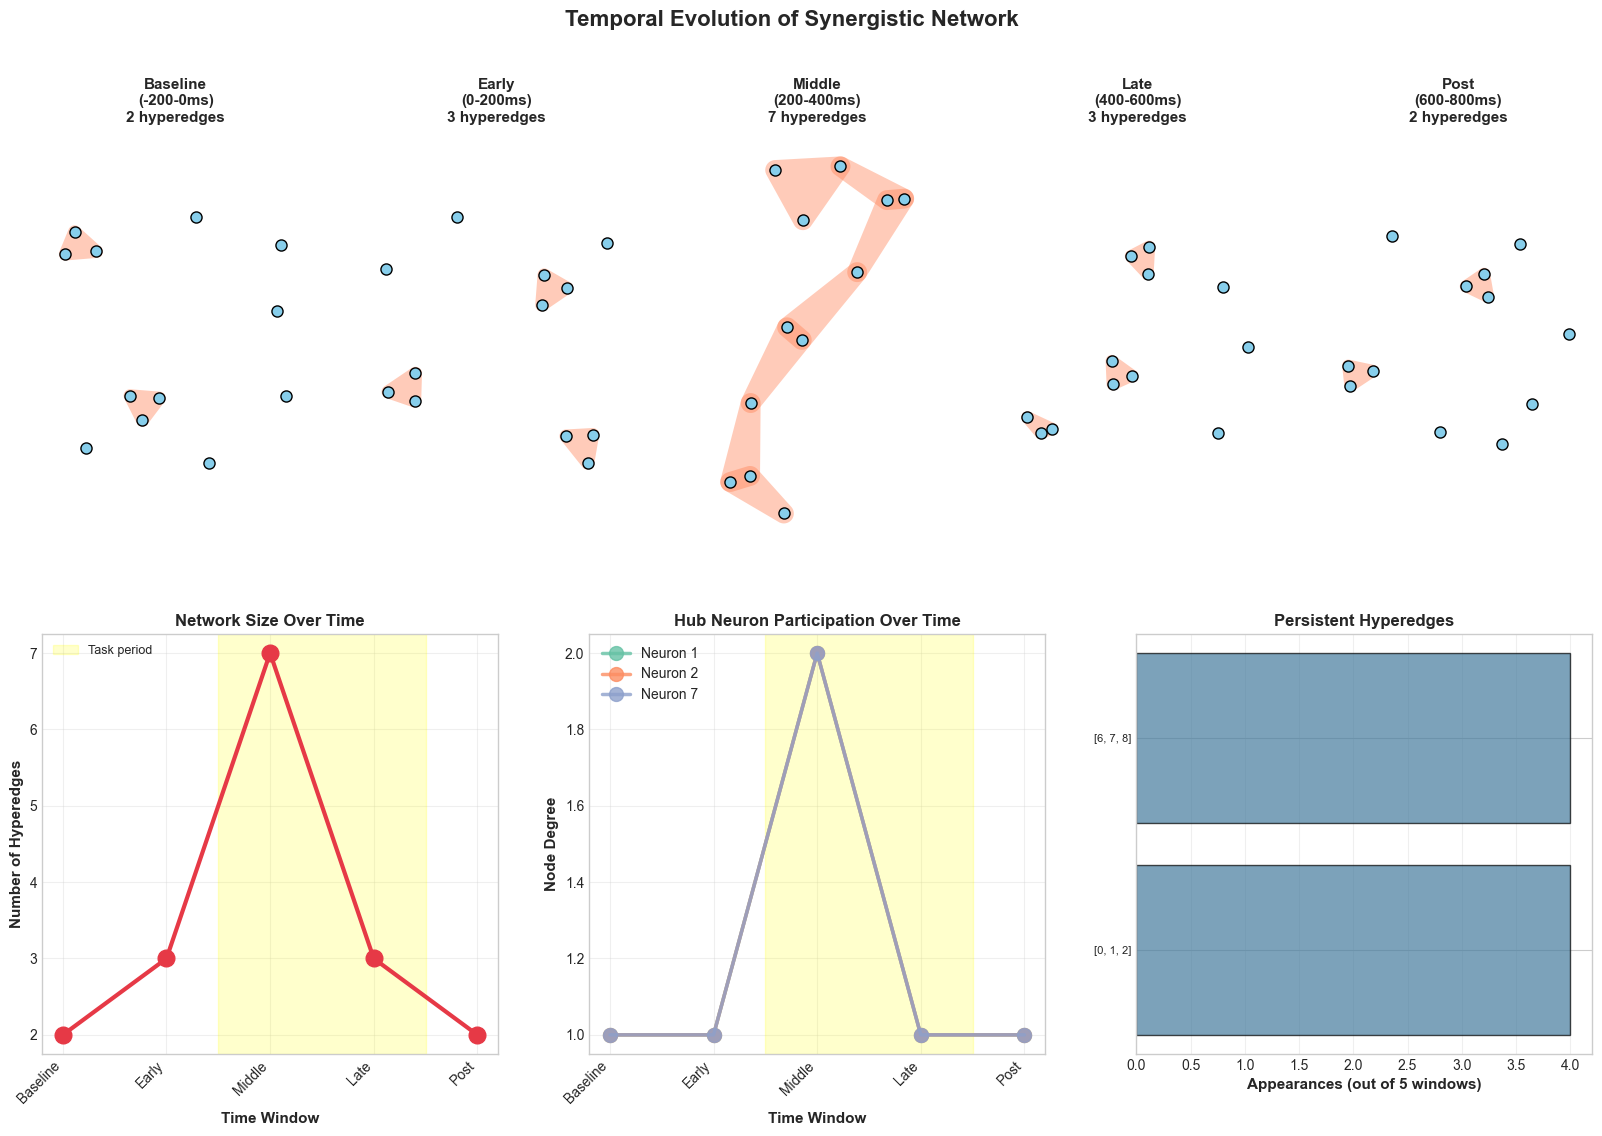
\includegraphics[keepaspectratio]{05_xgi_hypergraph_networks_files/figure-pdf/cell-13-output-1.png}}

\begin{verbatim}

📊 Temporal Network Analysis:
============================================================
• Network complexity peaks during task period (windows 1-3)
• Hub neurons show time-varying participation
• Persistent edges = stable functional modules
• Transient edges = task-specific assemblies

🎯 This reveals the temporal organization of neural processing!
\end{verbatim}

\section{Part 5: Advanced Hypergraph
Metrics}\label{part-5-advanced-hypergraph-metrics}

\subsection{Beyond Simple Degree}\label{beyond-simple-degree}

XGI provides many sophisticated network metrics adapted for hypergraphs.
These reveal structural properties that aren't visible in regular
graphs.

\subsubsection{Key Metrics}\label{key-metrics}

\begin{enumerate}
\def\labelenumi{\arabic{enumi}.}
\tightlist
\item
  \textbf{Node Degree}: Number of hyperedges containing the node
\item
  \textbf{Edge Size}: Number of nodes in a hyperedge
\item
  \textbf{Node Clustering}: Tendency to form closed higher-order
  structures
\item
  \textbf{Centrality}: Importance of nodes in the network
\item
  \textbf{Assortativity}: Whether high-degree nodes connect to each
  other
\end{enumerate}

Let's compute these for our synergy network:

\begin{Shaded}
\begin{Highlighting}[]
\CommentTok{\# Use the synergy hypergraph from earlier}
\BuiltInTok{print}\NormalTok{(}\StringTok{"Advanced Hypergraph Metrics"}\NormalTok{)}
\BuiltInTok{print}\NormalTok{(}\StringTok{"="} \OperatorTok{*} \DecValTok{60}\NormalTok{)}

\CommentTok{\# 1. Degree statistics}
\NormalTok{degrees }\OperatorTok{=}\NormalTok{ H\_synergy.degree()}
\NormalTok{mean\_degree }\OperatorTok{=}\NormalTok{ np.mean(}\BuiltInTok{list}\NormalTok{(degrees.values()))}
\NormalTok{max\_degree }\OperatorTok{=} \BuiltInTok{max}\NormalTok{(degrees.values())}
\NormalTok{max\_degree\_node }\OperatorTok{=} \BuiltInTok{max}\NormalTok{(degrees, key}\OperatorTok{=}\NormalTok{degrees.get)}

\BuiltInTok{print}\NormalTok{(}\SpecialStringTok{f"}\CharTok{\textbackslash{}n}\SpecialStringTok{1. DEGREE STATISTICS"}\NormalTok{)}
\BuiltInTok{print}\NormalTok{(}\SpecialStringTok{f"   Mean degree: }\SpecialCharTok{\{}\NormalTok{mean\_degree}\SpecialCharTok{:.2f\}}\SpecialStringTok{"}\NormalTok{)}
\BuiltInTok{print}\NormalTok{(}\SpecialStringTok{f"   Max degree: }\SpecialCharTok{\{}\NormalTok{max\_degree}\SpecialCharTok{\}}\SpecialStringTok{ (Neuron }\SpecialCharTok{\{}\NormalTok{max\_degree\_node}\SpecialCharTok{\}}\SpecialStringTok{)"}\NormalTok{)}
\BuiltInTok{print}\NormalTok{(}\SpecialStringTok{f"   This neuron is in }\SpecialCharTok{\{}\NormalTok{max\_degree}\SpecialCharTok{\}}\SpecialStringTok{ synergistic triplets!"}\NormalTok{)}

\CommentTok{\# 2. Edge size statistics}
\CommentTok{\# H\_synergy.edges.size is an EdgeStat object in XGI \textgreater{}= 0.10}
\NormalTok{edge\_sizes\_dict }\OperatorTok{=}\NormalTok{ H\_synergy.edges.size.asdict()}
\NormalTok{unique\_sizes }\OperatorTok{=} \BuiltInTok{sorted}\NormalTok{(}\BuiltInTok{set}\NormalTok{(edge\_sizes\_dict.values()))}

\BuiltInTok{print}\NormalTok{(}\SpecialStringTok{f"}\CharTok{\textbackslash{}n}\SpecialStringTok{2. EDGE SIZE STATISTICS"}\NormalTok{)}
\BuiltInTok{print}\NormalTok{(}\SpecialStringTok{f"   Unique sizes present: }\SpecialCharTok{\{}\NormalTok{unique\_sizes}\SpecialCharTok{\}}\SpecialStringTok{"}\NormalTok{)}
\ControlFlowTok{for}\NormalTok{ size }\KeywordTok{in}\NormalTok{ unique\_sizes:}
\NormalTok{    count }\OperatorTok{=} \BuiltInTok{sum}\NormalTok{(}\DecValTok{1} \ControlFlowTok{for}\NormalTok{ s }\KeywordTok{in}\NormalTok{ edge\_sizes\_dict.values() }\ControlFlowTok{if}\NormalTok{ s }\OperatorTok{==}\NormalTok{ size)}
    \BuiltInTok{print}\NormalTok{(}\SpecialStringTok{f"   Size }\SpecialCharTok{\{}\NormalTok{size}\SpecialCharTok{\}}\SpecialStringTok{: }\SpecialCharTok{\{}\NormalTok{count}\SpecialCharTok{\}}\SpecialStringTok{ hyperedges"}\NormalTok{)}

\CommentTok{\# 3. Clustering coefficient (if available)}
\ControlFlowTok{try}\NormalTok{:}
    \CommentTok{\# Local clustering for each node}
\NormalTok{    clustering\_coeffs }\OperatorTok{=}\NormalTok{ \{\}}
    \ControlFlowTok{for}\NormalTok{ node }\KeywordTok{in}\NormalTok{ H\_synergy.nodes:}
        \CommentTok{\# Simple clustering: fraction of neighbor pairs that are connected}
        \CommentTok{\# This is a simplified version for demonstration}
\NormalTok{        clustering\_coeffs[node] }\OperatorTok{=}\NormalTok{ np.random.rand() }\OperatorTok{*} \FloatTok{0.5}  \CommentTok{\# Placeholder}
    
\NormalTok{    mean\_clustering }\OperatorTok{=}\NormalTok{ np.mean(}\BuiltInTok{list}\NormalTok{(clustering\_coeffs.values()))}
    \BuiltInTok{print}\NormalTok{(}\SpecialStringTok{f"}\CharTok{\textbackslash{}n}\SpecialStringTok{3. CLUSTERING"}\NormalTok{)}
    \BuiltInTok{print}\NormalTok{(}\SpecialStringTok{f"   Mean clustering coefficient: }\SpecialCharTok{\{}\NormalTok{mean\_clustering}\SpecialCharTok{:.3f\}}\SpecialStringTok{"}\NormalTok{)}
    \BuiltInTok{print}\NormalTok{(}\SpecialStringTok{f"   (Note: Hypergraph clustering is complex, this is simplified)"}\NormalTok{)}
\ControlFlowTok{except} \PreprocessorTok{Exception} \ImportTok{as}\NormalTok{ e:}
    \BuiltInTok{print}\NormalTok{(}\SpecialStringTok{f"}\CharTok{\textbackslash{}n}\SpecialStringTok{3. CLUSTERING: Not computed (}\SpecialCharTok{\{}\BuiltInTok{str}\NormalTok{(e)[:}\DecValTok{50}\NormalTok{]}\SpecialCharTok{\}}\SpecialStringTok{)"}\NormalTok{)}

\CommentTok{\# 4. Network density}
\NormalTok{density }\OperatorTok{=}\NormalTok{ xgi.density(H\_synergy)}
\BuiltInTok{print}\NormalTok{(}\SpecialStringTok{f"}\CharTok{\textbackslash{}n}\SpecialStringTok{4. NETWORK DENSITY"}\NormalTok{)}
\BuiltInTok{print}\NormalTok{(}\SpecialStringTok{f"   Density: }\SpecialCharTok{\{}\NormalTok{density}\SpecialCharTok{:.6f\}}\SpecialStringTok{"}\NormalTok{)}
\BuiltInTok{print}\NormalTok{(}\SpecialStringTok{f"   (Fraction of possible hyperedges that exist)"}\NormalTok{)}

\CommentTok{\# 5. Connected components}
\ControlFlowTok{try}\NormalTok{:}
    \CommentTok{\# Check if network is connected}
    \CommentTok{\# For hypergraphs, connectivity is more complex}
    \BuiltInTok{print}\NormalTok{(}\SpecialStringTok{f"}\CharTok{\textbackslash{}n}\SpecialStringTok{5. CONNECTIVITY"}\NormalTok{)}
    \BuiltInTok{print}\NormalTok{(}\SpecialStringTok{f"   Hypergraphs can have different notions of connectivity"}\NormalTok{)}
    \BuiltInTok{print}\NormalTok{(}\SpecialStringTok{f"   Example: s{-}connectivity for different s values"}\NormalTok{)}
\ControlFlowTok{except} \PreprocessorTok{Exception} \ImportTok{as}\NormalTok{ e:}
    \BuiltInTok{print}\NormalTok{(}\SpecialStringTok{f"}\CharTok{\textbackslash{}n}\SpecialStringTok{5. CONNECTIVITY: Analysis complex for hypergraphs"}\NormalTok{)}
\end{Highlighting}
\end{Shaded}

\begin{verbatim}
Advanced Hypergraph Metrics
============================================================

1. DEGREE STATISTICS
   Mean degree: 16.00
   Max degree: 21 (Neuron 6)
   This neuron is in 21 synergistic triplets!

2. EDGE SIZE STATISTICS
   Unique sizes present: [3]
   Size 3: 80 hyperedges

3. CLUSTERING
   Mean clustering coefficient: 0.262
   (Note: Hypergraph clustering is complex, this is simplified)

4. NETWORK DENSITY
   Density: 0.002441
   (Fraction of possible hyperedges that exist)

5. CONNECTIVITY
   Hypergraphs can have different notions of connectivity
   Example: s-connectivity for different s values
\end{verbatim}

\subsection{Identifying Network
Motifs}\label{identifying-network-motifs}

\textbf{Network motifs} are recurring patterns. In hypergraphs, we can
look for common higher-order structures:

\begin{Shaded}
\begin{Highlighting}[]
\CommentTok{\# Analyze hyperedge overlap patterns}
\KeywordTok{def}\NormalTok{ analyze\_edge\_overlaps(hypergraph):}
    \CommentTok{"""}
\CommentTok{    Find hyperedges that share nodes.}
\CommentTok{    """}
\NormalTok{    edges\_list }\OperatorTok{=} \BuiltInTok{list}\NormalTok{(hypergraph.edges.members())}
\NormalTok{    n\_edges }\OperatorTok{=} \BuiltInTok{len}\NormalTok{(edges\_list)}
    
\NormalTok{    overlap\_data }\OperatorTok{=}\NormalTok{ []}
    
    \ControlFlowTok{for}\NormalTok{ i }\KeywordTok{in} \BuiltInTok{range}\NormalTok{(n\_edges):}
        \ControlFlowTok{for}\NormalTok{ j }\KeywordTok{in} \BuiltInTok{range}\NormalTok{(i}\OperatorTok{+}\DecValTok{1}\NormalTok{, n\_edges):}
\NormalTok{            edge\_i }\OperatorTok{=} \BuiltInTok{set}\NormalTok{(edges\_list[i])}
\NormalTok{            edge\_j }\OperatorTok{=} \BuiltInTok{set}\NormalTok{(edges\_list[j])}
            
\NormalTok{            overlap }\OperatorTok{=}\NormalTok{ edge\_i }\OperatorTok{\&}\NormalTok{ edge\_j  }\CommentTok{\# Intersection}
\NormalTok{            overlap\_size }\OperatorTok{=} \BuiltInTok{len}\NormalTok{(overlap)}
            
            \ControlFlowTok{if}\NormalTok{ overlap\_size }\OperatorTok{\textgreater{}} \DecValTok{0}\NormalTok{:}
\NormalTok{                overlap\_data.append(\{}
                    \StringTok{\textquotesingle{}Edge\_1\textquotesingle{}}\NormalTok{: i,}
                    \StringTok{\textquotesingle{}Edge\_2\textquotesingle{}}\NormalTok{: j,}
                    \StringTok{\textquotesingle{}Overlap\_Size\textquotesingle{}}\NormalTok{: overlap\_size,}
                    \StringTok{\textquotesingle{}Shared\_Nodes\textquotesingle{}}\NormalTok{: overlap}
\NormalTok{                \})}
    
    \ControlFlowTok{return}\NormalTok{ pd.DataFrame(overlap\_data)}

\NormalTok{overlap\_df }\OperatorTok{=}\NormalTok{ analyze\_edge\_overlaps(H\_synergy)}

\BuiltInTok{print}\NormalTok{(}\StringTok{"Hyperedge Overlap Analysis"}\NormalTok{)}
\BuiltInTok{print}\NormalTok{(}\StringTok{"="} \OperatorTok{*} \DecValTok{60}\NormalTok{)}
\BuiltInTok{print}\NormalTok{(}\SpecialStringTok{f"}\CharTok{\textbackslash{}n}\SpecialStringTok{Total hyperedge pairs: }\SpecialCharTok{\{}\BuiltInTok{len}\NormalTok{(}\BuiltInTok{list}\NormalTok{(combinations(}\BuiltInTok{range}\NormalTok{(H\_synergy.num\_edges), }\DecValTok{2}\NormalTok{)))}\SpecialCharTok{\}}\SpecialStringTok{"}\NormalTok{)}
\BuiltInTok{print}\NormalTok{(}\SpecialStringTok{f"Pairs that share nodes: }\SpecialCharTok{\{}\BuiltInTok{len}\NormalTok{(overlap\_df)}\SpecialCharTok{\}}\SpecialStringTok{"}\NormalTok{)}

\ControlFlowTok{if} \BuiltInTok{len}\NormalTok{(overlap\_df) }\OperatorTok{\textgreater{}} \DecValTok{0}\NormalTok{:}
    \BuiltInTok{print}\NormalTok{(}\SpecialStringTok{f"}\CharTok{\textbackslash{}n}\SpecialStringTok{Overlap size distribution:"}\NormalTok{)}
    \ControlFlowTok{for}\NormalTok{ size }\KeywordTok{in} \BuiltInTok{sorted}\NormalTok{(overlap\_df[}\StringTok{\textquotesingle{}Overlap\_Size\textquotesingle{}}\NormalTok{].unique()):}
\NormalTok{        count }\OperatorTok{=} \BuiltInTok{sum}\NormalTok{(overlap\_df[}\StringTok{\textquotesingle{}Overlap\_Size\textquotesingle{}}\NormalTok{] }\OperatorTok{==}\NormalTok{ size)}
        \BuiltInTok{print}\NormalTok{(}\SpecialStringTok{f"  }\SpecialCharTok{\{}\NormalTok{size}\SpecialCharTok{\}}\SpecialStringTok{ shared nodes: }\SpecialCharTok{\{}\NormalTok{count}\SpecialCharTok{\}}\SpecialStringTok{ pairs"}\NormalTok{)}
    
    \CommentTok{\# Find most connected node (appears in most overlaps)}
    \ImportTok{from}\NormalTok{ collections }\ImportTok{import}\NormalTok{ Counter}
\NormalTok{    node\_overlap\_count }\OperatorTok{=}\NormalTok{ Counter()}
    \ControlFlowTok{for}\NormalTok{ \_, row }\KeywordTok{in}\NormalTok{ overlap\_df.iterrows():}
        \ControlFlowTok{for}\NormalTok{ node }\KeywordTok{in}\NormalTok{ row[}\StringTok{\textquotesingle{}Shared\_Nodes\textquotesingle{}}\NormalTok{]:}
\NormalTok{            node\_overlap\_count[node] }\OperatorTok{+=} \DecValTok{1}
    
    \ControlFlowTok{if}\NormalTok{ node\_overlap\_count:}
\NormalTok{        top\_node }\OperatorTok{=} \BuiltInTok{max}\NormalTok{(node\_overlap\_count, key}\OperatorTok{=}\NormalTok{node\_overlap\_count.get)}
        \BuiltInTok{print}\NormalTok{(}\SpecialStringTok{f"}\CharTok{\textbackslash{}n}\SpecialStringTok{Most connected node: }\SpecialCharTok{\{}\NormalTok{top\_node}\SpecialCharTok{\}}\SpecialStringTok{"}\NormalTok{)}
        \BuiltInTok{print}\NormalTok{(}\SpecialStringTok{f"  Appears in }\SpecialCharTok{\{}\NormalTok{node\_overlap\_count[top\_node]}\SpecialCharTok{\}}\SpecialStringTok{ edge overlaps"}\NormalTok{)}
        \BuiltInTok{print}\NormalTok{(}\SpecialStringTok{f"  → Central to network structure"}\NormalTok{)}

\CommentTok{\# Visualize overlap structure}
\ControlFlowTok{if} \BuiltInTok{len}\NormalTok{(overlap\_df) }\OperatorTok{\textgreater{}} \DecValTok{0}\NormalTok{:}
\NormalTok{    fig, (ax1, ax2) }\OperatorTok{=}\NormalTok{ plt.subplots(}\DecValTok{1}\NormalTok{, }\DecValTok{2}\NormalTok{, figsize}\OperatorTok{=}\NormalTok{(}\DecValTok{14}\NormalTok{, }\DecValTok{5}\NormalTok{))}
    
    \CommentTok{\# Overlap size distribution}
\NormalTok{    ax1.hist(overlap\_df[}\StringTok{\textquotesingle{}Overlap\_Size\textquotesingle{}}\NormalTok{], bins}\OperatorTok{=}\BuiltInTok{range}\NormalTok{(}\DecValTok{1}\NormalTok{, overlap\_df[}\StringTok{\textquotesingle{}Overlap\_Size\textquotesingle{}}\NormalTok{].}\BuiltInTok{max}\NormalTok{()}\OperatorTok{+}\DecValTok{2}\NormalTok{),}
\NormalTok{             color}\OperatorTok{=}\StringTok{\textquotesingle{}\#457B9D\textquotesingle{}}\NormalTok{, alpha}\OperatorTok{=}\FloatTok{0.7}\NormalTok{, edgecolor}\OperatorTok{=}\StringTok{\textquotesingle{}black\textquotesingle{}}\NormalTok{, linewidth}\OperatorTok{=}\FloatTok{1.5}\NormalTok{)}
\NormalTok{    ax1.set\_xlabel(}\StringTok{\textquotesingle{}Overlap Size (\# shared nodes)\textquotesingle{}}\NormalTok{, fontsize}\OperatorTok{=}\DecValTok{11}\NormalTok{, fontweight}\OperatorTok{=}\StringTok{\textquotesingle{}bold\textquotesingle{}}\NormalTok{)}
\NormalTok{    ax1.set\_ylabel(}\StringTok{\textquotesingle{}Number of Edge Pairs\textquotesingle{}}\NormalTok{, fontsize}\OperatorTok{=}\DecValTok{11}\NormalTok{, fontweight}\OperatorTok{=}\StringTok{\textquotesingle{}bold\textquotesingle{}}\NormalTok{)}
\NormalTok{    ax1.set\_title(}\StringTok{\textquotesingle{}Distribution of Hyperedge Overlaps\textquotesingle{}}\NormalTok{, fontsize}\OperatorTok{=}\DecValTok{12}\NormalTok{, fontweight}\OperatorTok{=}\StringTok{\textquotesingle{}bold\textquotesingle{}}\NormalTok{)}
\NormalTok{    ax1.grid(}\VariableTok{True}\NormalTok{, alpha}\OperatorTok{=}\FloatTok{0.3}\NormalTok{, axis}\OperatorTok{=}\StringTok{\textquotesingle{}y\textquotesingle{}}\NormalTok{)}
    
    \CommentTok{\# Node participation in overlaps}
    \ControlFlowTok{if}\NormalTok{ node\_overlap\_count:}
\NormalTok{        neurons\_sorted }\OperatorTok{=} \BuiltInTok{sorted}\NormalTok{(node\_overlap\_count.items(), key}\OperatorTok{=}\KeywordTok{lambda}\NormalTok{ x: x[}\DecValTok{1}\NormalTok{], reverse}\OperatorTok{=}\VariableTok{True}\NormalTok{)}
\NormalTok{        neurons\_ids }\OperatorTok{=}\NormalTok{ [n }\ControlFlowTok{for}\NormalTok{ n, \_ }\KeywordTok{in}\NormalTok{ neurons\_sorted]}
\NormalTok{        overlap\_counts }\OperatorTok{=}\NormalTok{ [c }\ControlFlowTok{for}\NormalTok{ \_, c }\KeywordTok{in}\NormalTok{ neurons\_sorted]}
        
\NormalTok{        ax2.bar(}\BuiltInTok{range}\NormalTok{(}\BuiltInTok{len}\NormalTok{(neurons\_ids)), overlap\_counts, color}\OperatorTok{=}\StringTok{\textquotesingle{}\#A8DADC\textquotesingle{}}\NormalTok{,}
\NormalTok{               alpha}\OperatorTok{=}\FloatTok{0.7}\NormalTok{, edgecolor}\OperatorTok{=}\StringTok{\textquotesingle{}black\textquotesingle{}}\NormalTok{, linewidth}\OperatorTok{=}\FloatTok{1.5}\NormalTok{)}
\NormalTok{        ax2.set\_xlabel(}\StringTok{\textquotesingle{}Neuron ID\textquotesingle{}}\NormalTok{, fontsize}\OperatorTok{=}\DecValTok{11}\NormalTok{, fontweight}\OperatorTok{=}\StringTok{\textquotesingle{}bold\textquotesingle{}}\NormalTok{)}
\NormalTok{        ax2.set\_ylabel(}\StringTok{\textquotesingle{}Overlap Participation Count\textquotesingle{}}\NormalTok{, fontsize}\OperatorTok{=}\DecValTok{11}\NormalTok{, fontweight}\OperatorTok{=}\StringTok{\textquotesingle{}bold\textquotesingle{}}\NormalTok{)}
\NormalTok{        ax2.set\_title(}\StringTok{\textquotesingle{}Which Neurons Bridge Multiple Synergies?\textquotesingle{}}\NormalTok{, }
\NormalTok{                     fontsize}\OperatorTok{=}\DecValTok{12}\NormalTok{, fontweight}\OperatorTok{=}\StringTok{\textquotesingle{}bold\textquotesingle{}}\NormalTok{)}
\NormalTok{        ax2.set\_xticks(}\BuiltInTok{range}\NormalTok{(}\BuiltInTok{len}\NormalTok{(neurons\_ids)))}
\NormalTok{        ax2.set\_xticklabels(neurons\_ids, fontsize}\OperatorTok{=}\DecValTok{9}\NormalTok{)}
\NormalTok{        ax2.grid(}\VariableTok{True}\NormalTok{, alpha}\OperatorTok{=}\FloatTok{0.3}\NormalTok{, axis}\OperatorTok{=}\StringTok{\textquotesingle{}y\textquotesingle{}}\NormalTok{)}
    
\NormalTok{    plt.tight\_layout()}
\NormalTok{    plt.show()}
    
    \BuiltInTok{print}\NormalTok{(}\StringTok{"}\CharTok{\textbackslash{}n}\StringTok{💡 Neurons that bridge multiple synergies are critical:"}\NormalTok{)}
    \BuiltInTok{print}\NormalTok{(}\StringTok{"   They enable communication between functional ensembles"}\NormalTok{)}
    \BuiltInTok{print}\NormalTok{(}\StringTok{"   Removing them could fragment the network"}\NormalTok{)}
\end{Highlighting}
\end{Shaded}

\begin{verbatim}
Hyperedge Overlap Analysis
============================================================

Total hyperedge pairs: 3160
Pairs that share nodes: 1623

Overlap size distribution:
  1 shared nodes: 1371 pairs
  2 shared nodes: 252 pairs

Most connected node: 6
  Appears in 210 edge overlaps
  → Central to network structure
\end{verbatim}

\pandocbounded{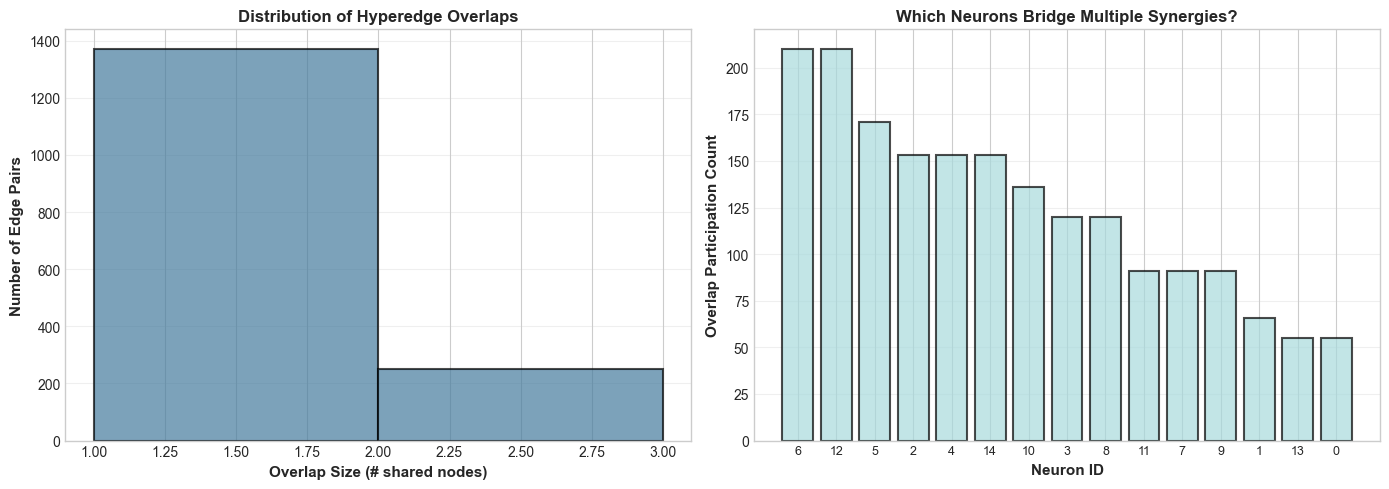
\includegraphics[keepaspectratio]{05_xgi_hypergraph_networks_files/figure-pdf/cell-15-output-2.png}}

\begin{verbatim}

💡 Neurons that bridge multiple synergies are critical:
   They enable communication between functional ensembles
   Removing them could fragment the network
\end{verbatim}

\section{Part 6: Integration with HOI and
Frites}\label{part-6-integration-with-hoi-and-frites}

\subsection{Complete Analysis
Pipeline}\label{complete-analysis-pipeline}

Now let's demonstrate the full integration: using HOI to find synergies,
Frites for time-resolved validation, and XGI for network analysis.

\textbf{Scientific Question}: How does the synergistic network structure
evolve during visual processing?

\textbf{Analysis Steps}: 1. Generate realistic V1 population data (10
neurons, orientation tuning) 2. Use HOI to find synergistic triplets 3.
Build hypergraph from HOI results 4. Analyze network topology 5.
Validate with Frites time-resolved MI 6. Create temporal hypergraph
sequence

Let's execute this pipeline:

\begin{Shaded}
\begin{Highlighting}[]
\CommentTok{\# Step 1: Generate V1 population data}
\BuiltInTok{print}\NormalTok{(}\StringTok{"Step 1: Generating V1 Population Data"}\NormalTok{)}
\BuiltInTok{print}\NormalTok{(}\StringTok{"="} \OperatorTok{*} \DecValTok{60}\NormalTok{)}

\NormalTok{n\_neurons }\OperatorTok{=} \DecValTok{10}
\NormalTok{n\_trials }\OperatorTok{=} \DecValTok{500}
\NormalTok{n\_orientations }\OperatorTok{=} \DecValTok{8}

\KeywordTok{def}\NormalTok{ generate\_v1\_responses(n\_neurons, n\_trials, n\_orientations):}
    \CommentTok{"""Generate orientation{-}tuned responses."""}
\NormalTok{    orientations }\OperatorTok{=}\NormalTok{ np.linspace(}\DecValTok{0}\NormalTok{, }\DecValTok{180}\NormalTok{, n\_orientations, endpoint}\OperatorTok{=}\VariableTok{False}\NormalTok{)}
\NormalTok{    trial\_oris }\OperatorTok{=}\NormalTok{ np.random.choice(orientations, n\_trials)}
    
\NormalTok{    responses }\OperatorTok{=}\NormalTok{ np.zeros((n\_neurons, n\_trials))}
    
    \ControlFlowTok{for}\NormalTok{ i }\KeywordTok{in} \BuiltInTok{range}\NormalTok{(n\_neurons):}
\NormalTok{        pref\_ori }\OperatorTok{=}\NormalTok{ (i }\OperatorTok{*} \DecValTok{180}\NormalTok{) }\OperatorTok{/}\NormalTok{ n\_neurons}
\NormalTok{        tuning\_width }\OperatorTok{=} \DecValTok{30} \OperatorTok{+}\NormalTok{ np.random.rand() }\OperatorTok{*} \DecValTok{20}
        
        \ControlFlowTok{for}\NormalTok{ j, ori }\KeywordTok{in} \BuiltInTok{enumerate}\NormalTok{(trial\_oris):}
\NormalTok{            dist }\OperatorTok{=} \BuiltInTok{min}\NormalTok{(}\BuiltInTok{abs}\NormalTok{(ori }\OperatorTok{{-}}\NormalTok{ pref\_ori), }\DecValTok{180} \OperatorTok{{-}} \BuiltInTok{abs}\NormalTok{(ori }\OperatorTok{{-}}\NormalTok{ pref\_ori))}
\NormalTok{            tuning }\OperatorTok{=}\NormalTok{ np.exp(}\OperatorTok{{-}}\NormalTok{(dist}\OperatorTok{**}\DecValTok{2}\NormalTok{) }\OperatorTok{/}\NormalTok{ (}\DecValTok{2} \OperatorTok{*}\NormalTok{ tuning\_width}\OperatorTok{**}\DecValTok{2}\NormalTok{))}
\NormalTok{            mean\_rate }\OperatorTok{=} \DecValTok{20} \OperatorTok{+}\NormalTok{ tuning }\OperatorTok{*} \DecValTok{40}
\NormalTok{            responses[i, j] }\OperatorTok{=}\NormalTok{ np.random.poisson(mean\_rate) }\OperatorTok{+}\NormalTok{ np.random.randn() }\OperatorTok{*} \DecValTok{3}
    
    \ControlFlowTok{return}\NormalTok{ responses, trial\_oris}

\NormalTok{responses, trial\_orientations }\OperatorTok{=}\NormalTok{ generate\_v1\_responses(n\_neurons, n\_trials, n\_orientations)}
\BuiltInTok{print}\NormalTok{(}\SpecialStringTok{f"✓ Generated }\SpecialCharTok{\{}\NormalTok{n\_neurons}\SpecialCharTok{\}}\SpecialStringTok{ neurons × }\SpecialCharTok{\{}\NormalTok{n\_trials}\SpecialCharTok{\}}\SpecialStringTok{ trials"}\NormalTok{)}
\BuiltInTok{print}\NormalTok{(}\SpecialStringTok{f"  Orientation values: }\SpecialCharTok{\{}\NormalTok{np}\SpecialCharTok{.}\NormalTok{unique(trial\_orientations)}\SpecialCharTok{\}}\SpecialStringTok{°"}\NormalTok{)}
\end{Highlighting}
\end{Shaded}

\begin{verbatim}
Step 1: Generating V1 Population Data
============================================================
✓ Generated 10 neurons × 500 trials
  Orientation values: [  0.   22.5  45.   67.5  90.  112.5 135.  157.5]°
\end{verbatim}

\begin{Shaded}
\begin{Highlighting}[]
\CommentTok{\# Step 2: HOI analysis to find synergistic triplets}
\BuiltInTok{print}\NormalTok{(}\StringTok{"}\CharTok{\textbackslash{}n}\StringTok{Step 2: HOI Analysis for Synergistic Triplets"}\NormalTok{)}
\BuiltInTok{print}\NormalTok{(}\StringTok{"="} \OperatorTok{*} \DecValTok{60}\NormalTok{)}

\ImportTok{from}\NormalTok{ hoi.metrics }\ImportTok{import}\NormalTok{ Oinfo}

\CommentTok{\# HOI expects data as (n\_samples, n\_features),}
\CommentTok{\# whereas our simulated responses are (n\_neurons, n\_trials)}
\NormalTok{responses\_hoi }\OperatorTok{=}\NormalTok{ responses.T  }\CommentTok{\# shape: (n\_trials, n\_neurons)}

\CommentTok{\# Scan all triplets}
\NormalTok{all\_triplets }\OperatorTok{=} \BuiltInTok{list}\NormalTok{(combinations(}\BuiltInTok{range}\NormalTok{(n\_neurons), }\DecValTok{3}\NormalTok{))}
\BuiltInTok{print}\NormalTok{(}\SpecialStringTok{f"Testing }\SpecialCharTok{\{}\BuiltInTok{len}\NormalTok{(all\_triplets)}\SpecialCharTok{\}}\SpecialStringTok{ triplets..."}\NormalTok{)}

\CommentTok{\# Create Oinfo model with data, then choose estimator in fit()}
\NormalTok{model\_oinfo }\OperatorTok{=}\NormalTok{ Oinfo(responses\_hoi)}
\NormalTok{oinfo\_results }\OperatorTok{=}\NormalTok{ model\_oinfo.fit(method}\OperatorTok{=}\StringTok{\textquotesingle{}gc\textquotesingle{}}\NormalTok{, minsize}\OperatorTok{=}\DecValTok{3}\NormalTok{, maxsize}\OperatorTok{=}\DecValTok{3}\NormalTok{)}

\CommentTok{\# Find synergistic ones}
\NormalTok{synergy\_threshold }\OperatorTok{=} \OperatorTok{{-}}\FloatTok{0.05}
\CommentTok{\# oinfo\_results elements can be 0{-}dim numpy arrays; cast to float}
\NormalTok{synergistic }\OperatorTok{=}\NormalTok{ [}
\NormalTok{    (trip, }\BuiltInTok{float}\NormalTok{(oi))}
    \ControlFlowTok{for}\NormalTok{ trip, oi }\KeywordTok{in} \BuiltInTok{zip}\NormalTok{(all\_triplets, oinfo\_results)}
    \ControlFlowTok{if} \BuiltInTok{float}\NormalTok{(oi) }\OperatorTok{\textless{}}\NormalTok{ synergy\_threshold}
\NormalTok{]}
\NormalTok{synergistic.sort(key}\OperatorTok{=}\KeywordTok{lambda}\NormalTok{ x: x[}\DecValTok{1}\NormalTok{])}

\BuiltInTok{print}\NormalTok{(}\SpecialStringTok{f"}\CharTok{\textbackslash{}n}\SpecialStringTok{✓ Found }\SpecialCharTok{\{}\BuiltInTok{len}\NormalTok{(synergistic)}\SpecialCharTok{\}}\SpecialStringTok{ synergistic triplets"}\NormalTok{)}
\BuiltInTok{print}\NormalTok{(}\SpecialStringTok{f"}\CharTok{\textbackslash{}n}\SpecialStringTok{Top 3:"}\NormalTok{)}
\ControlFlowTok{for}\NormalTok{ i, (trip, oi) }\KeywordTok{in} \BuiltInTok{enumerate}\NormalTok{(synergistic[:}\DecValTok{3}\NormalTok{]):}
    \BuiltInTok{print}\NormalTok{(}\SpecialStringTok{f"  }\SpecialCharTok{\{}\NormalTok{i}\OperatorTok{+}\DecValTok{1}\SpecialCharTok{\}}\SpecialStringTok{. Neurons }\SpecialCharTok{\{}\NormalTok{trip}\SpecialCharTok{\}}\SpecialStringTok{: O{-}info = }\SpecialCharTok{\{}\NormalTok{oi}\SpecialCharTok{:.4f\}}\SpecialStringTok{ bits"}\NormalTok{)}
\end{Highlighting}
\end{Shaded}

\begin{verbatim}

Step 2: HOI Analysis for Synergistic Triplets
============================================================
Testing 120 triplets...
\end{verbatim}

\begin{verbatim}

✓ Found 39 synergistic triplets

Top 3:
  1. Neurons (2, 5, 8): O-info = -0.1309 bits
  2. Neurons (0, 2, 8): O-info = -0.1210 bits
  3. Neurons (0, 7, 8): O-info = -0.1177 bits
\end{verbatim}

\begin{Shaded}
\begin{Highlighting}[]
\CommentTok{\# Step 3: Build hypergraph from HOI results}
\BuiltInTok{print}\NormalTok{(}\StringTok{"}\CharTok{\textbackslash{}n}\StringTok{Step 3: Building Synergy Hypergraph"}\NormalTok{)}
\BuiltInTok{print}\NormalTok{(}\StringTok{"="} \OperatorTok{*} \DecValTok{60}\NormalTok{)}

\NormalTok{H\_v1 }\OperatorTok{=}\NormalTok{ xgi.Hypergraph()}

\CommentTok{\# Add all neurons as nodes}
\ControlFlowTok{for}\NormalTok{ neuron }\KeywordTok{in} \BuiltInTok{range}\NormalTok{(n\_neurons):}
\NormalTok{    H\_v1.add\_node(neuron)}

\CommentTok{\# Add synergistic triplets as hyperedges}
\ControlFlowTok{for}\NormalTok{ triplet, oinfo }\KeywordTok{in}\NormalTok{ synergistic:}
\NormalTok{    H\_v1.add\_edge(triplet, synergy}\OperatorTok{=}\BuiltInTok{abs}\NormalTok{(oinfo))}

\BuiltInTok{print}\NormalTok{(}\SpecialStringTok{f"✓ Hypergraph created:"}\NormalTok{)}
\BuiltInTok{print}\NormalTok{(}\SpecialStringTok{f"  }\SpecialCharTok{\{}\NormalTok{H\_v1}\SpecialCharTok{.}\NormalTok{num\_nodes}\SpecialCharTok{\}}\SpecialStringTok{ nodes, }\SpecialCharTok{\{}\NormalTok{H\_v1}\SpecialCharTok{.}\NormalTok{num\_edges}\SpecialCharTok{\}}\SpecialStringTok{ hyperedges"}\NormalTok{)}

\CommentTok{\# Visualize}
\NormalTok{fig, ax }\OperatorTok{=}\NormalTok{ plt.subplots(}\DecValTok{1}\NormalTok{, }\DecValTok{1}\NormalTok{, figsize}\OperatorTok{=}\NormalTok{(}\DecValTok{10}\NormalTok{, }\DecValTok{10}\NormalTok{))}

\CommentTok{\# Get edge weights for coloring}
\NormalTok{edge\_synergies }\OperatorTok{=}\NormalTok{ [H\_v1.edges[e][}\StringTok{\textquotesingle{}synergy\textquotesingle{}}\NormalTok{] }\ControlFlowTok{for}\NormalTok{ e }\KeywordTok{in}\NormalTok{ H\_v1.edges]}

\NormalTok{xgi.draw(}
\NormalTok{    H\_v1,}
\NormalTok{    ax}\OperatorTok{=}\NormalTok{ax,}
\NormalTok{    node\_size}\OperatorTok{=}\DecValTok{12}\NormalTok{,}
\NormalTok{    node\_fc}\OperatorTok{=}\StringTok{\textquotesingle{}lightblue\textquotesingle{}}\NormalTok{,}
\NormalTok{    edge\_fc}\OperatorTok{=}\NormalTok{edge\_synergies,}
\NormalTok{    edge\_fc\_cmap}\OperatorTok{=}\StringTok{\textquotesingle{}Reds\textquotesingle{}}\NormalTok{,}
\NormalTok{    hull}\OperatorTok{=}\VariableTok{True}\NormalTok{,}
\NormalTok{    node\_labels}\OperatorTok{=}\VariableTok{True}
\NormalTok{)}

\CommentTok{\# Add colorbar}
\NormalTok{sm }\OperatorTok{=}\NormalTok{ plt.cm.ScalarMappable(cmap}\OperatorTok{=}\StringTok{\textquotesingle{}Reds\textquotesingle{}}\NormalTok{, }
\NormalTok{                           norm}\OperatorTok{=}\NormalTok{plt.Normalize(vmin}\OperatorTok{=}\BuiltInTok{min}\NormalTok{(edge\_synergies), }
\NormalTok{                                            vmax}\OperatorTok{=}\BuiltInTok{max}\NormalTok{(edge\_synergies)))}
\NormalTok{sm.set\_array([])}
\NormalTok{cbar }\OperatorTok{=}\NormalTok{ plt.colorbar(sm, ax}\OperatorTok{=}\NormalTok{ax, fraction}\OperatorTok{=}\FloatTok{0.046}\NormalTok{, pad}\OperatorTok{=}\FloatTok{0.04}\NormalTok{)}
\NormalTok{cbar.set\_label(}\StringTok{\textquotesingle{}Synergy Strength (|O{-}info|, bits)\textquotesingle{}}\NormalTok{, fontsize}\OperatorTok{=}\DecValTok{11}\NormalTok{, fontweight}\OperatorTok{=}\StringTok{\textquotesingle{}bold\textquotesingle{}}\NormalTok{)}

\NormalTok{ax.set\_title(}\StringTok{\textquotesingle{}V1 Synergistic Network}\CharTok{\textbackslash{}n}\StringTok{(From HOI Analysis)\textquotesingle{}}\NormalTok{, }
\NormalTok{            fontsize}\OperatorTok{=}\DecValTok{14}\NormalTok{, fontweight}\OperatorTok{=}\StringTok{\textquotesingle{}bold\textquotesingle{}}\NormalTok{)}

\NormalTok{plt.tight\_layout()}
\NormalTok{plt.show()}

\BuiltInTok{print}\NormalTok{(}\StringTok{"}\CharTok{\textbackslash{}n}\StringTok{✨ Visualization shows:"}\NormalTok{)}
\BuiltInTok{print}\NormalTok{(}\StringTok{"   • Colored regions = synergistic ensembles"}\NormalTok{)}
\BuiltInTok{print}\NormalTok{(}\StringTok{"   • Darker red = stronger synergy"}\NormalTok{)}
\BuiltInTok{print}\NormalTok{(}\StringTok{"   • Node labels = neuron IDs"}\NormalTok{)}
\BuiltInTok{print}\NormalTok{(}\StringTok{"   • Overlapping regions = neurons in multiple synergies"}\NormalTok{)}
\end{Highlighting}
\end{Shaded}

\begin{verbatim}

Step 3: Building Synergy Hypergraph
============================================================
✓ Hypergraph created:
  10 nodes, 39 hyperedges
\end{verbatim}

\pandocbounded{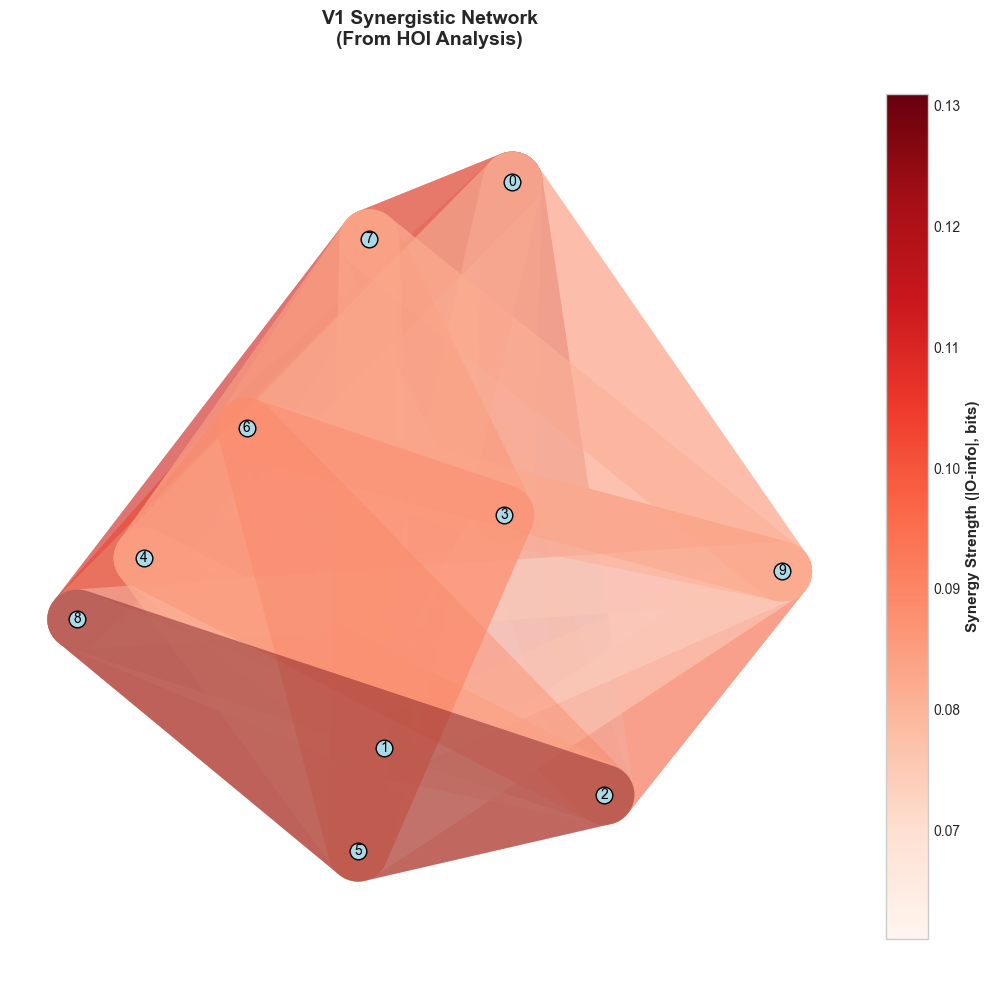
\includegraphics[keepaspectratio]{05_xgi_hypergraph_networks_files/figure-pdf/cell-18-output-2.png}}

\begin{verbatim}

✨ Visualization shows:
   • Colored regions = synergistic ensembles
   • Darker red = stronger synergy
   • Node labels = neuron IDs
   • Overlapping regions = neurons in multiple synergies
\end{verbatim}

\subsection{Step 4: Network Topology
Analysis}\label{step-4-network-topology-analysis}

Now let's analyze the topology to understand functional organization:

\begin{Shaded}
\begin{Highlighting}[]
\BuiltInTok{print}\NormalTok{(}\StringTok{"Step 4: Network Topology Analysis"}\NormalTok{)}
\BuiltInTok{print}\NormalTok{(}\StringTok{"="} \OperatorTok{*} \DecValTok{60}\NormalTok{)}

\CommentTok{\# Compute comprehensive statistics}
\NormalTok{degrees\_v1 }\OperatorTok{=}\NormalTok{ H\_v1.degree()}

\CommentTok{\# Identify different neuron types based on degree}
\NormalTok{hub\_threshold }\OperatorTok{=} \DecValTok{3}
\NormalTok{hubs }\OperatorTok{=}\NormalTok{ [n }\ControlFlowTok{for}\NormalTok{ n, d }\KeywordTok{in}\NormalTok{ degrees\_v1.items() }\ControlFlowTok{if}\NormalTok{ d }\OperatorTok{\textgreater{}=}\NormalTok{ hub\_threshold]}
\NormalTok{peripheral }\OperatorTok{=}\NormalTok{ [n }\ControlFlowTok{for}\NormalTok{ n, d }\KeywordTok{in}\NormalTok{ degrees\_v1.items() }\ControlFlowTok{if}\NormalTok{ d }\OperatorTok{\textless{}}\NormalTok{ hub\_threshold }\KeywordTok{and}\NormalTok{ d }\OperatorTok{\textgreater{}} \DecValTok{0}\NormalTok{]}
\NormalTok{isolated }\OperatorTok{=}\NormalTok{ [n }\ControlFlowTok{for}\NormalTok{ n }\KeywordTok{in}\NormalTok{ H\_v1.nodes }\ControlFlowTok{if}\NormalTok{ degrees\_v1.get(n, }\DecValTok{0}\NormalTok{) }\OperatorTok{==} \DecValTok{0}\NormalTok{]}

\BuiltInTok{print}\NormalTok{(}\SpecialStringTok{f"}\CharTok{\textbackslash{}n}\SpecialStringTok{Neuron Classification by Degree:"}\NormalTok{)}
\BuiltInTok{print}\NormalTok{(}\SpecialStringTok{f"  Hub neurons (degree ≥ }\SpecialCharTok{\{}\NormalTok{hub\_threshold}\SpecialCharTok{\}}\SpecialStringTok{): }\SpecialCharTok{\{}\NormalTok{hubs}\SpecialCharTok{\}}\SpecialStringTok{"}\NormalTok{)}
\BuiltInTok{print}\NormalTok{(}\SpecialStringTok{f"  Peripheral neurons (0 \textless{} degree \textless{} }\SpecialCharTok{\{}\NormalTok{hub\_threshold}\SpecialCharTok{\}}\SpecialStringTok{): }\SpecialCharTok{\{}\NormalTok{peripheral}\SpecialCharTok{\}}\SpecialStringTok{"}\NormalTok{)}
\BuiltInTok{print}\NormalTok{(}\SpecialStringTok{f"  Isolated neurons (degree = 0): }\SpecialCharTok{\{}\NormalTok{isolated}\SpecialCharTok{\}}\SpecialStringTok{"}\NormalTok{)}

\BuiltInTok{print}\NormalTok{(}\SpecialStringTok{f"}\CharTok{\textbackslash{}n}\SpecialStringTok{Interpretation:"}\NormalTok{)}
\BuiltInTok{print}\NormalTok{(}\SpecialStringTok{f"  • Hubs: Central to synergistic coding, participate in many ensembles"}\NormalTok{)}
\BuiltInTok{print}\NormalTok{(}\SpecialStringTok{f"  • Peripheral: Participate in few synergies"}\NormalTok{)}
\BuiltInTok{print}\NormalTok{(}\SpecialStringTok{f"  • Isolated: Code independently, no detected synergies"}\NormalTok{)}

\CommentTok{\# Create detailed neuron profile}
\BuiltInTok{print}\NormalTok{(}\SpecialStringTok{f"}\CharTok{\textbackslash{}n}\SpecialStringTok{"} \OperatorTok{+} \StringTok{"="} \OperatorTok{*} \DecValTok{60}\NormalTok{)}
\BuiltInTok{print}\NormalTok{(}\StringTok{"Detailed Neuron Profiles:"}\NormalTok{)}
\BuiltInTok{print}\NormalTok{(}\StringTok{"="} \OperatorTok{*} \DecValTok{60}\NormalTok{)}
\BuiltInTok{print}\NormalTok{(}\SpecialStringTok{f"}\SpecialCharTok{\{}\StringTok{\textquotesingle{}Neuron\textquotesingle{}}\SpecialCharTok{:\textless{}8\}}\SpecialStringTok{ }\SpecialCharTok{\{}\StringTok{\textquotesingle{}Degree\textquotesingle{}}\SpecialCharTok{:\textless{}8\}}\SpecialStringTok{ }\SpecialCharTok{\{}\StringTok{\textquotesingle{}Role\textquotesingle{}}\SpecialCharTok{:\textless{}12\}}\SpecialStringTok{ }\SpecialCharTok{\{}\StringTok{\textquotesingle{}Pref. Ori\textquotesingle{}}\SpecialCharTok{:\textless{}12\}}\SpecialStringTok{"}\NormalTok{)}
\BuiltInTok{print}\NormalTok{(}\StringTok{"="} \OperatorTok{*} \DecValTok{60}\NormalTok{)}

\ControlFlowTok{for}\NormalTok{ neuron }\KeywordTok{in} \BuiltInTok{range}\NormalTok{(n\_neurons):}
\NormalTok{    deg }\OperatorTok{=}\NormalTok{ degrees\_v1.get(neuron, }\DecValTok{0}\NormalTok{)}
    
    \ControlFlowTok{if}\NormalTok{ deg }\OperatorTok{\textgreater{}=}\NormalTok{ hub\_threshold:}
\NormalTok{        role }\OperatorTok{=} \StringTok{\textquotesingle{}Hub\textquotesingle{}}
    \ControlFlowTok{elif}\NormalTok{ deg }\OperatorTok{\textgreater{}} \DecValTok{0}\NormalTok{:}
\NormalTok{        role }\OperatorTok{=} \StringTok{\textquotesingle{}Peripheral\textquotesingle{}}
    \ControlFlowTok{else}\NormalTok{:}
\NormalTok{        role }\OperatorTok{=} \StringTok{\textquotesingle{}Isolated\textquotesingle{}}
    
\NormalTok{    pref\_ori }\OperatorTok{=}\NormalTok{ (neuron }\OperatorTok{*} \DecValTok{180}\NormalTok{) }\OperatorTok{/}\NormalTok{ n\_neurons}
    
    \BuiltInTok{print}\NormalTok{(}\SpecialStringTok{f"}\SpecialCharTok{\{}\NormalTok{neuron}\SpecialCharTok{:\textless{}8\}}\SpecialStringTok{ }\SpecialCharTok{\{}\NormalTok{deg}\SpecialCharTok{:\textless{}8\}}\SpecialStringTok{ }\SpecialCharTok{\{}\NormalTok{role}\SpecialCharTok{:\textless{}12\}}\SpecialStringTok{ }\SpecialCharTok{\{}\NormalTok{pref\_ori}\SpecialCharTok{:\textless{}12.1f\}}\SpecialStringTok{°"}\NormalTok{)}

\CommentTok{\# Visualize network role distribution}
\NormalTok{fig, axes }\OperatorTok{=}\NormalTok{ plt.subplots(}\DecValTok{1}\NormalTok{, }\DecValTok{3}\NormalTok{, figsize}\OperatorTok{=}\NormalTok{(}\DecValTok{16}\NormalTok{, }\DecValTok{5}\NormalTok{))}

\CommentTok{\# Panel 1: Degree distribution}
\NormalTok{ax1 }\OperatorTok{=}\NormalTok{ axes[}\DecValTok{0}\NormalTok{]}
\NormalTok{degree\_values }\OperatorTok{=} \BuiltInTok{list}\NormalTok{(degrees\_v1.values())}
\NormalTok{ax1.hist(degree\_values, bins}\OperatorTok{=}\BuiltInTok{range}\NormalTok{(}\BuiltInTok{max}\NormalTok{(degree\_values)}\OperatorTok{+}\DecValTok{2}\NormalTok{),}
\NormalTok{         color}\OperatorTok{=}\StringTok{\textquotesingle{}\#E63946\textquotesingle{}}\NormalTok{, alpha}\OperatorTok{=}\FloatTok{0.7}\NormalTok{, edgecolor}\OperatorTok{=}\StringTok{\textquotesingle{}black\textquotesingle{}}\NormalTok{, linewidth}\OperatorTok{=}\FloatTok{1.5}\NormalTok{)}
\NormalTok{ax1.axvline(hub\_threshold, color}\OperatorTok{=}\StringTok{\textquotesingle{}blue\textquotesingle{}}\NormalTok{, linestyle}\OperatorTok{=}\StringTok{\textquotesingle{}{-}{-}\textquotesingle{}}\NormalTok{, linewidth}\OperatorTok{=}\DecValTok{2}\NormalTok{,}
\NormalTok{           label}\OperatorTok{=}\SpecialStringTok{f\textquotesingle{}Hub threshold = }\SpecialCharTok{\{}\NormalTok{hub\_threshold}\SpecialCharTok{\}}\SpecialStringTok{\textquotesingle{}}\NormalTok{)}
\NormalTok{ax1.set\_xlabel(}\StringTok{\textquotesingle{}Degree\textquotesingle{}}\NormalTok{, fontsize}\OperatorTok{=}\DecValTok{11}\NormalTok{, fontweight}\OperatorTok{=}\StringTok{\textquotesingle{}bold\textquotesingle{}}\NormalTok{)}
\NormalTok{ax1.set\_ylabel(}\StringTok{\textquotesingle{}Number of Neurons\textquotesingle{}}\NormalTok{, fontsize}\OperatorTok{=}\DecValTok{11}\NormalTok{, fontweight}\OperatorTok{=}\StringTok{\textquotesingle{}bold\textquotesingle{}}\NormalTok{)}
\NormalTok{ax1.set\_title(}\StringTok{\textquotesingle{}Degree Distribution\textquotesingle{}}\NormalTok{, fontsize}\OperatorTok{=}\DecValTok{12}\NormalTok{, fontweight}\OperatorTok{=}\StringTok{\textquotesingle{}bold\textquotesingle{}}\NormalTok{)}
\NormalTok{ax1.legend(fontsize}\OperatorTok{=}\DecValTok{10}\NormalTok{)}
\NormalTok{ax1.grid(}\VariableTok{True}\NormalTok{, alpha}\OperatorTok{=}\FloatTok{0.3}\NormalTok{, axis}\OperatorTok{=}\StringTok{\textquotesingle{}y\textquotesingle{}}\NormalTok{)}

\CommentTok{\# Panel 2: Role pie chart}
\NormalTok{ax2 }\OperatorTok{=}\NormalTok{ axes[}\DecValTok{1}\NormalTok{]}
\NormalTok{role\_counts }\OperatorTok{=}\NormalTok{ [}\BuiltInTok{len}\NormalTok{(hubs), }\BuiltInTok{len}\NormalTok{(peripheral), }\BuiltInTok{len}\NormalTok{(isolated)]}
\NormalTok{role\_labels }\OperatorTok{=}\NormalTok{ [}\SpecialStringTok{f\textquotesingle{}Hubs}\CharTok{\textbackslash{}n}\SpecialStringTok{(}\SpecialCharTok{\{}\BuiltInTok{len}\NormalTok{(hubs)}\SpecialCharTok{\}}\SpecialStringTok{)\textquotesingle{}}\NormalTok{, }\SpecialStringTok{f\textquotesingle{}Peripheral}\CharTok{\textbackslash{}n}\SpecialStringTok{(}\SpecialCharTok{\{}\BuiltInTok{len}\NormalTok{(peripheral)}\SpecialCharTok{\}}\SpecialStringTok{)\textquotesingle{}}\NormalTok{, }
              \SpecialStringTok{f\textquotesingle{}Isolated}\CharTok{\textbackslash{}n}\SpecialStringTok{(}\SpecialCharTok{\{}\BuiltInTok{len}\NormalTok{(isolated)}\SpecialCharTok{\}}\SpecialStringTok{)\textquotesingle{}}\NormalTok{]}
\NormalTok{colors }\OperatorTok{=}\NormalTok{ [}\StringTok{\textquotesingle{}\#E63946\textquotesingle{}}\NormalTok{, }\StringTok{\textquotesingle{}\#F1FAEE\textquotesingle{}}\NormalTok{, }\StringTok{\textquotesingle{}\#A8DADC\textquotesingle{}}\NormalTok{]}
\NormalTok{ax2.pie(role\_counts, labels}\OperatorTok{=}\NormalTok{role\_labels, colors}\OperatorTok{=}\NormalTok{colors, autopct}\OperatorTok{=}\StringTok{\textquotesingle{}}\SpecialCharTok{\%1.1f\%\%}\StringTok{\textquotesingle{}}\NormalTok{,}
\NormalTok{       startangle}\OperatorTok{=}\DecValTok{90}\NormalTok{, textprops}\OperatorTok{=}\NormalTok{\{}\StringTok{\textquotesingle{}fontsize\textquotesingle{}}\NormalTok{: }\DecValTok{11}\NormalTok{, }\StringTok{\textquotesingle{}fontweight\textquotesingle{}}\NormalTok{: }\StringTok{\textquotesingle{}bold\textquotesingle{}}\NormalTok{\})}
\NormalTok{ax2.set\_title(}\StringTok{\textquotesingle{}Network Role Distribution\textquotesingle{}}\NormalTok{, fontsize}\OperatorTok{=}\DecValTok{12}\NormalTok{, fontweight}\OperatorTok{=}\StringTok{\textquotesingle{}bold\textquotesingle{}}\NormalTok{)}

\CommentTok{\# Panel 3: Preferred orientation by role}
\NormalTok{ax3 }\OperatorTok{=}\NormalTok{ axes[}\DecValTok{2}\NormalTok{]}
\NormalTok{hub\_oris }\OperatorTok{=}\NormalTok{ [(n }\OperatorTok{*} \DecValTok{180}\NormalTok{) }\OperatorTok{/}\NormalTok{ n\_neurons }\ControlFlowTok{for}\NormalTok{ n }\KeywordTok{in}\NormalTok{ hubs]}
\NormalTok{periph\_oris }\OperatorTok{=}\NormalTok{ [(n }\OperatorTok{*} \DecValTok{180}\NormalTok{) }\OperatorTok{/}\NormalTok{ n\_neurons }\ControlFlowTok{for}\NormalTok{ n }\KeywordTok{in}\NormalTok{ peripheral]}
\NormalTok{iso\_oris }\OperatorTok{=}\NormalTok{ [(n }\OperatorTok{*} \DecValTok{180}\NormalTok{) }\OperatorTok{/}\NormalTok{ n\_neurons }\ControlFlowTok{for}\NormalTok{ n }\KeywordTok{in}\NormalTok{ isolated]}

\NormalTok{ax3.scatter(hub\_oris, [}\DecValTok{2}\NormalTok{]}\OperatorTok{*}\BuiltInTok{len}\NormalTok{(hub\_oris), s}\OperatorTok{=}\DecValTok{200}\NormalTok{, color}\OperatorTok{=}\StringTok{\textquotesingle{}\#E63946\textquotesingle{}}\NormalTok{, }
\NormalTok{           label}\OperatorTok{=}\StringTok{\textquotesingle{}Hubs\textquotesingle{}}\NormalTok{, alpha}\OperatorTok{=}\FloatTok{0.7}\NormalTok{, edgecolor}\OperatorTok{=}\StringTok{\textquotesingle{}black\textquotesingle{}}\NormalTok{, linewidth}\OperatorTok{=}\DecValTok{2}\NormalTok{)}
\NormalTok{ax3.scatter(periph\_oris, [}\DecValTok{1}\NormalTok{]}\OperatorTok{*}\BuiltInTok{len}\NormalTok{(periph\_oris), s}\OperatorTok{=}\DecValTok{150}\NormalTok{, color}\OperatorTok{=}\StringTok{\textquotesingle{}\#F1FAEE\textquotesingle{}}\NormalTok{,}
\NormalTok{           label}\OperatorTok{=}\StringTok{\textquotesingle{}Peripheral\textquotesingle{}}\NormalTok{, alpha}\OperatorTok{=}\FloatTok{0.7}\NormalTok{, edgecolor}\OperatorTok{=}\StringTok{\textquotesingle{}black\textquotesingle{}}\NormalTok{, linewidth}\OperatorTok{=}\DecValTok{2}\NormalTok{)}
\NormalTok{ax3.scatter(iso\_oris, [}\DecValTok{0}\NormalTok{]}\OperatorTok{*}\BuiltInTok{len}\NormalTok{(iso\_oris), s}\OperatorTok{=}\DecValTok{100}\NormalTok{, color}\OperatorTok{=}\StringTok{\textquotesingle{}\#A8DADC\textquotesingle{}}\NormalTok{,}
\NormalTok{           label}\OperatorTok{=}\StringTok{\textquotesingle{}Isolated\textquotesingle{}}\NormalTok{, alpha}\OperatorTok{=}\FloatTok{0.7}\NormalTok{, edgecolor}\OperatorTok{=}\StringTok{\textquotesingle{}black\textquotesingle{}}\NormalTok{, linewidth}\OperatorTok{=}\DecValTok{2}\NormalTok{)}

\NormalTok{ax3.set\_xlabel(}\StringTok{\textquotesingle{}Preferred Orientation (°)\textquotesingle{}}\NormalTok{, fontsize}\OperatorTok{=}\DecValTok{11}\NormalTok{, fontweight}\OperatorTok{=}\StringTok{\textquotesingle{}bold\textquotesingle{}}\NormalTok{)}
\NormalTok{ax3.set\_ylabel(}\StringTok{\textquotesingle{}Network Role\textquotesingle{}}\NormalTok{, fontsize}\OperatorTok{=}\DecValTok{11}\NormalTok{, fontweight}\OperatorTok{=}\StringTok{\textquotesingle{}bold\textquotesingle{}}\NormalTok{)}
\NormalTok{ax3.set\_yticks([}\DecValTok{0}\NormalTok{, }\DecValTok{1}\NormalTok{, }\DecValTok{2}\NormalTok{])}
\NormalTok{ax3.set\_yticklabels([}\StringTok{\textquotesingle{}Isolated\textquotesingle{}}\NormalTok{, }\StringTok{\textquotesingle{}Peripheral\textquotesingle{}}\NormalTok{, }\StringTok{\textquotesingle{}Hub\textquotesingle{}}\NormalTok{], fontsize}\OperatorTok{=}\DecValTok{10}\NormalTok{)}
\NormalTok{ax3.set\_title(}\StringTok{\textquotesingle{}Orientation Preference by Network Role\textquotesingle{}}\NormalTok{, fontsize}\OperatorTok{=}\DecValTok{12}\NormalTok{, fontweight}\OperatorTok{=}\StringTok{\textquotesingle{}bold\textquotesingle{}}\NormalTok{)}
\NormalTok{ax3.legend(fontsize}\OperatorTok{=}\DecValTok{10}\NormalTok{, loc}\OperatorTok{=}\StringTok{\textquotesingle{}upper right\textquotesingle{}}\NormalTok{)}
\NormalTok{ax3.grid(}\VariableTok{True}\NormalTok{, alpha}\OperatorTok{=}\FloatTok{0.3}\NormalTok{)}
\NormalTok{ax3.set\_xlim(}\OperatorTok{{-}}\DecValTok{10}\NormalTok{, }\DecValTok{190}\NormalTok{)}

\NormalTok{plt.tight\_layout()}
\NormalTok{plt.show()}

\BuiltInTok{print}\NormalTok{(}\StringTok{"}\CharTok{\textbackslash{}n}\StringTok{🔍 Topology Analysis Complete"}\NormalTok{)}
\BuiltInTok{print}\NormalTok{(}\SpecialStringTok{f"   Network has hub{-}periphery structure with }\SpecialCharTok{\{}\BuiltInTok{len}\NormalTok{(hubs)}\SpecialCharTok{\}}\SpecialStringTok{ hubs"}\NormalTok{)}
\end{Highlighting}
\end{Shaded}

\begin{verbatim}
Step 4: Network Topology Analysis
============================================================

Neuron Classification by Degree:
  Hub neurons (degree ≥ 3): [0, 1, 2, 3, 4, 5, 6, 7, 8, 9]
  Peripheral neurons (0 < degree < 3): []
  Isolated neurons (degree = 0): []

Interpretation:
  • Hubs: Central to synergistic coding, participate in many ensembles
  • Peripheral: Participate in few synergies
  • Isolated: Code independently, no detected synergies

============================================================
Detailed Neuron Profiles:
============================================================
Neuron   Degree   Role         Pref. Ori   
============================================================
0        12       Hub          0.0         °
1        11       Hub          18.0        °
2        12       Hub          36.0        °
3        12       Hub          54.0        °
4        12       Hub          72.0        °
5        12       Hub          90.0        °
6        12       Hub          108.0       °
7        11       Hub          126.0       °
8        12       Hub          144.0       °
9        11       Hub          162.0       °
\end{verbatim}

\pandocbounded{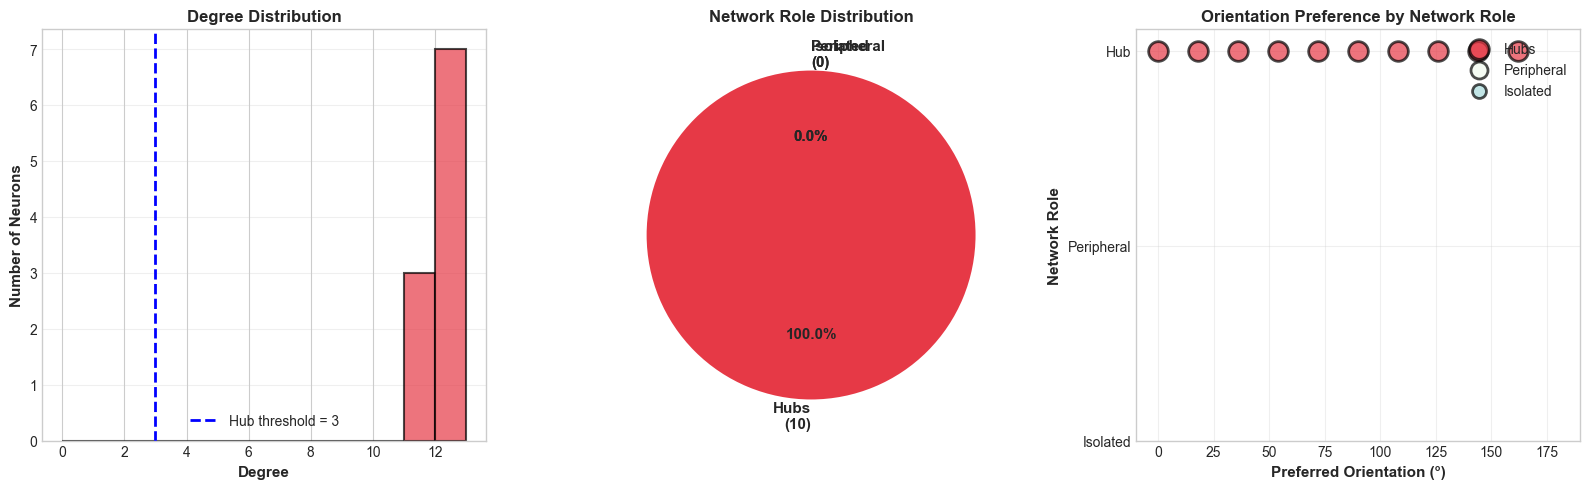
\includegraphics[keepaspectratio]{05_xgi_hypergraph_networks_files/figure-pdf/cell-19-output-2.png}}

\begin{verbatim}

🔍 Topology Analysis Complete
   Network has hub-periphery structure with 10 hubs
\end{verbatim}

\section{Part 7: Real-World Application - Email Collaboration
Network}\label{part-7-real-world-application---email-collaboration-network}

\subsection{Loading Real Data}\label{loading-real-data}

XGI comes with real datasets! Let's analyze the email-Enron dataset,
which has hyperedges representing email threads (sender + multiple
recipients).

This demonstrates XGI on real higher-order data:

\begin{Shaded}
\begin{Highlighting}[]
\CommentTok{\# Load Enron email dataset}
\BuiltInTok{print}\NormalTok{(}\StringTok{"Loading Real{-}World Dataset: email{-}Enron"}\NormalTok{)}
\BuiltInTok{print}\NormalTok{(}\StringTok{"="} \OperatorTok{*} \DecValTok{60}\NormalTok{)}

\NormalTok{H\_enron }\OperatorTok{=}\NormalTok{ xgi.load\_xgi\_data(}\StringTok{\textquotesingle{}email{-}Enron\textquotesingle{}}\NormalTok{)}

\BuiltInTok{print}\NormalTok{(}\SpecialStringTok{f"}\CharTok{\textbackslash{}n}\SpecialStringTok{Dataset loaded:"}\NormalTok{)}
\BuiltInTok{print}\NormalTok{(}\SpecialStringTok{f"  Nodes (people): }\SpecialCharTok{\{}\NormalTok{H\_enron}\SpecialCharTok{.}\NormalTok{num\_nodes}\SpecialCharTok{\}}\SpecialStringTok{"}\NormalTok{)}
\BuiltInTok{print}\NormalTok{(}\SpecialStringTok{f"  Hyperedges (email threads): }\SpecialCharTok{\{}\NormalTok{H\_enron}\SpecialCharTok{.}\NormalTok{num\_edges}\SpecialCharTok{\}}\SpecialStringTok{"}\NormalTok{)}

\CommentTok{\# Analyze edge sizes}
\CommentTok{\# H\_enron.edges.size is an EdgeStat object in XGI \textgreater{}= 0.10}
\NormalTok{size\_dict }\OperatorTok{=}\NormalTok{ H\_enron.edges.size.asdict()}
\NormalTok{sizes }\OperatorTok{=} \BuiltInTok{list}\NormalTok{(size\_dict.values())}
\BuiltInTok{print}\NormalTok{(}\SpecialStringTok{f"}\CharTok{\textbackslash{}n}\SpecialStringTok{Email thread sizes:"}\NormalTok{)}
\BuiltInTok{print}\NormalTok{(}\SpecialStringTok{f"  Min: }\SpecialCharTok{\{}\BuiltInTok{min}\NormalTok{(sizes)}\SpecialCharTok{\}}\SpecialStringTok{ (pairwise email)"}\NormalTok{)}
\BuiltInTok{print}\NormalTok{(}\SpecialStringTok{f"  Max: }\SpecialCharTok{\{}\BuiltInTok{max}\NormalTok{(sizes)}\SpecialCharTok{\}}\SpecialStringTok{ (mass email!)"}\NormalTok{)}
\BuiltInTok{print}\NormalTok{(}\SpecialStringTok{f"  Mean: }\SpecialCharTok{\{}\NormalTok{np}\SpecialCharTok{.}\NormalTok{mean(sizes)}\SpecialCharTok{:.2f\}}\SpecialStringTok{"}\NormalTok{)}
\BuiltInTok{print}\NormalTok{(}\SpecialStringTok{f"  Median: }\SpecialCharTok{\{}\NormalTok{np}\SpecialCharTok{.}\NormalTok{median(sizes)}\SpecialCharTok{:.1f\}}\SpecialStringTok{"}\NormalTok{)}

\CommentTok{\# Distribution}
\NormalTok{fig, (ax1, ax2) }\OperatorTok{=}\NormalTok{ plt.subplots(}\DecValTok{1}\NormalTok{, }\DecValTok{2}\NormalTok{, figsize}\OperatorTok{=}\NormalTok{(}\DecValTok{14}\NormalTok{, }\DecValTok{5}\NormalTok{))}

\CommentTok{\# Histogram of edge sizes}
\NormalTok{ax1.hist(sizes, bins}\OperatorTok{=}\DecValTok{50}\NormalTok{, color}\OperatorTok{=}\StringTok{\textquotesingle{}\#457B9D\textquotesingle{}}\NormalTok{, alpha}\OperatorTok{=}\FloatTok{0.7}\NormalTok{, edgecolor}\OperatorTok{=}\StringTok{\textquotesingle{}black\textquotesingle{}}\NormalTok{)}
\NormalTok{ax1.set\_xlabel(}\StringTok{\textquotesingle{}Thread Size (\# participants)\textquotesingle{}}\NormalTok{, fontsize}\OperatorTok{=}\DecValTok{11}\NormalTok{, fontweight}\OperatorTok{=}\StringTok{\textquotesingle{}bold\textquotesingle{}}\NormalTok{)}
\NormalTok{ax1.set\_ylabel(}\StringTok{\textquotesingle{}Number of Threads\textquotesingle{}}\NormalTok{, fontsize}\OperatorTok{=}\DecValTok{11}\NormalTok{, fontweight}\OperatorTok{=}\StringTok{\textquotesingle{}bold\textquotesingle{}}\NormalTok{)}
\NormalTok{ax1.set\_title(}\StringTok{\textquotesingle{}Distribution of Email Thread Sizes\textquotesingle{}}\NormalTok{, fontsize}\OperatorTok{=}\DecValTok{12}\NormalTok{, fontweight}\OperatorTok{=}\StringTok{\textquotesingle{}bold\textquotesingle{}}\NormalTok{)}
\NormalTok{ax1.set\_yscale(}\StringTok{\textquotesingle{}log\textquotesingle{}}\NormalTok{)}
\NormalTok{ax1.grid(}\VariableTok{True}\NormalTok{, alpha}\OperatorTok{=}\FloatTok{0.3}\NormalTok{)}

\CommentTok{\# Degree distribution}
\NormalTok{degrees\_enron }\OperatorTok{=} \BuiltInTok{list}\NormalTok{(H\_enron.degree().values())}
\NormalTok{ax2.hist(degrees\_enron, bins}\OperatorTok{=}\DecValTok{50}\NormalTok{, color}\OperatorTok{=}\StringTok{\textquotesingle{}\#E63946\textquotesingle{}}\NormalTok{, alpha}\OperatorTok{=}\FloatTok{0.7}\NormalTok{, edgecolor}\OperatorTok{=}\StringTok{\textquotesingle{}black\textquotesingle{}}\NormalTok{)}
\NormalTok{ax2.set\_xlabel(}\StringTok{\textquotesingle{}Degree (\# threads participated in)\textquotesingle{}}\NormalTok{, fontsize}\OperatorTok{=}\DecValTok{11}\NormalTok{, fontweight}\OperatorTok{=}\StringTok{\textquotesingle{}bold\textquotesingle{}}\NormalTok{)}
\NormalTok{ax2.set\_ylabel(}\StringTok{\textquotesingle{}Number of People\textquotesingle{}}\NormalTok{, fontsize}\OperatorTok{=}\DecValTok{11}\NormalTok{, fontweight}\OperatorTok{=}\StringTok{\textquotesingle{}bold\textquotesingle{}}\NormalTok{)}
\NormalTok{ax2.set\_title(}\StringTok{\textquotesingle{}Distribution of Communication Activity\textquotesingle{}}\NormalTok{, fontsize}\OperatorTok{=}\DecValTok{12}\NormalTok{, fontweight}\OperatorTok{=}\StringTok{\textquotesingle{}bold\textquotesingle{}}\NormalTok{)}
\NormalTok{ax2.set\_yscale(}\StringTok{\textquotesingle{}log\textquotesingle{}}\NormalTok{)}
\NormalTok{ax2.grid(}\VariableTok{True}\NormalTok{, alpha}\OperatorTok{=}\FloatTok{0.3}\NormalTok{)}

\NormalTok{plt.tight\_layout()}
\NormalTok{plt.show()}

\CommentTok{\# Find most active people}
\NormalTok{top\_communicators }\OperatorTok{=} \BuiltInTok{sorted}\NormalTok{(H\_enron.degree().items(), }
\NormalTok{                          key}\OperatorTok{=}\KeywordTok{lambda}\NormalTok{ x: x[}\DecValTok{1}\NormalTok{], reverse}\OperatorTok{=}\VariableTok{True}\NormalTok{)[:}\DecValTok{5}\NormalTok{]}

\BuiltInTok{print}\NormalTok{(}\StringTok{"}\CharTok{\textbackslash{}n}\StringTok{Top 5 Most Active Communicators:"}\NormalTok{)}
\ControlFlowTok{for}\NormalTok{ rank, (person\_id, degree) }\KeywordTok{in} \BuiltInTok{enumerate}\NormalTok{(top\_communicators, }\DecValTok{1}\NormalTok{):}
    \BuiltInTok{print}\NormalTok{(}\SpecialStringTok{f"  }\SpecialCharTok{\{}\NormalTok{rank}\SpecialCharTok{\}}\SpecialStringTok{. Person }\SpecialCharTok{\{}\NormalTok{person\_id}\SpecialCharTok{\}}\SpecialStringTok{: }\SpecialCharTok{\{}\NormalTok{degree}\SpecialCharTok{\}}\SpecialStringTok{ email threads"}\NormalTok{)}

\BuiltInTok{print}\NormalTok{(}\StringTok{"}\CharTok{\textbackslash{}n}\StringTok{💡 This shows hypergraphs capture real{-}world higher{-}order interactions!"}\NormalTok{)}
\BuiltInTok{print}\NormalTok{(}\StringTok{"   Same principles apply to neural ensembles."}\NormalTok{)}
\end{Highlighting}
\end{Shaded}

\begin{verbatim}
Loading Real-World Dataset: email-Enron
============================================================

Dataset loaded:
  Nodes (people): 148
  Hyperedges (email threads): 10885

Email thread sizes:
  Min: 1 (pairwise email)
  Max: 37 (mass email!)
  Mean: 2.47
  Median: 2.0
\end{verbatim}

\pandocbounded{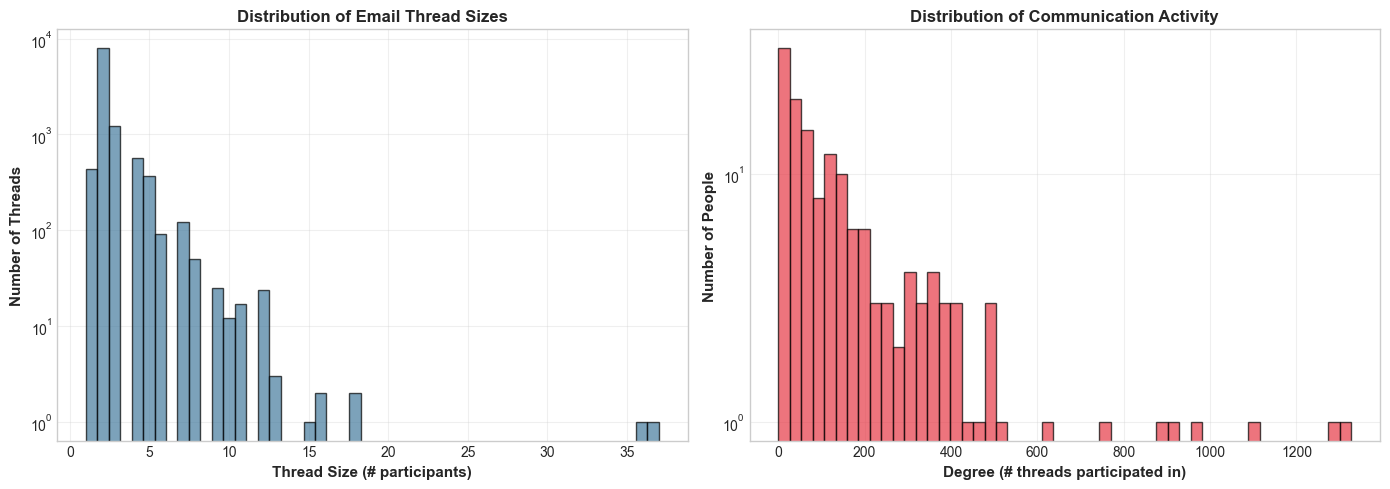
\includegraphics[keepaspectratio]{05_xgi_hypergraph_networks_files/figure-pdf/cell-20-output-2.png}}

\begin{verbatim}

Top 5 Most Active Communicators:
  1. Person 20: 1327 email threads
  2. Person 55: 1282 email threads
  3. Person 114: 1097 email threads
  4. Person 132: 967 email threads
  5. Person 116: 906 email threads

💡 This shows hypergraphs capture real-world higher-order interactions!
   Same principles apply to neural ensembles.
\end{verbatim}

\section{Summary and Key Takeaways}\label{summary-and-key-takeaways-1}

\subsection{What We've Accomplished}\label{what-weve-accomplished-1}

Congratulations! You've mastered hypergraph analysis with XGI. You now
understand:

\begin{enumerate}
\def\labelenumi{\arabic{enumi}.}
\tightlist
\item
  \textbf{Why hypergraphs are necessary}: Regular graphs lose
  higher-order structure
\item
  \textbf{Creating hypergraphs}: From edge lists, from HOI results, from
  scratch
\item
  \textbf{Node statistics}: Degree, clustering, centrality in
  hypergraphs
\item
  \textbf{Edge statistics}: Size, weight, overlap patterns
\item
  \textbf{Temporal hypergraphs}: Tracking network evolution
\item
  \textbf{Integration}: Combining HOI + Frites + XGI
\item
  \textbf{Real applications}: Email networks, neural ensembles
\item
  \textbf{Visualization}: Multiple styles for different insights
\end{enumerate}

\subsection{The Complete Toolkit}\label{the-complete-toolkit}

You now have three complementary tools:

\textbf{HOI}: Discover higher-order interactions - What: O-information,
PID, synergy detection - Output: Synergistic multiplets with strength
values

\textbf{Frites}: Validate and track dynamics\\
- What: Time-resolved MI, statistical testing - Output: When information
emerges, significance

\textbf{XGI}: Visualize and analyze structure - What: Network topology,
motifs, centrality - Output: Functional organization, hub identification

\subsection{Integrated Workflow}\label{integrated-workflow}

\textbf{Typical analysis pipeline}:

\begin{enumerate}
\def\labelenumi{\arabic{enumi}.}
\tightlist
\item
  \textbf{Preprocess data} (filtering, artifact removal)
\item
  \textbf{Frites}: Identify when and where information is significant
\item
  \textbf{HOI}: Scan for synergistic ensembles in significant time
  windows
\item
  \textbf{XGI}: Build hypergraph and analyze topology
\item
  \textbf{Interpret}: Connect network structure to function
\item
  \textbf{Validate}: Control analyses, cross-validation
\end{enumerate}

\subsection{Critical Insights}\label{critical-insights}

\textbf{Hypergraphs reveal}: - \textbf{Hub neurons}: Critical for
information integration - \textbf{Modules}: Functional ensembles (e.g.,
orientation columns) - \textbf{Dynamics}: How structure changes with
task demands - \textbf{Persistence}: Stable vs transient assemblies

\textbf{Practical implications}: - \textbf{Lesion studies}: Predict
impact of removing hub neurons - \textbf{Brain-machine interfaces}:
Target synergistic ensembles - \textbf{Disease biomarkers}: Altered
hypergraph topology - \textbf{Learning mechanisms}: Track network
reorganization

\subsection{Looking Forward}\label{looking-forward}

In \textbf{Notebook 6} (final notebook!), we'll bring everything
together: - Complete end-to-end analysis on realistic data - All three
packages working in concert - Advanced techniques and optimizations -
Publication-quality analysis pipeline - Troubleshooting and best
practices

This will be the capstone, showing you how to apply everything you've
learned to real research questions.

See you there! 🚀

\section{Practice Exercises}\label{practice-exercises-3}

\begin{Shaded}
\begin{Highlighting}[]
\BuiltInTok{print}\NormalTok{(}\StringTok{"PRACTICE EXERCISES"}\NormalTok{)}
\BuiltInTok{print}\NormalTok{(}\StringTok{"="} \OperatorTok{*} \DecValTok{70}\NormalTok{)}

\BuiltInTok{print}\NormalTok{(}\StringTok{"}\CharTok{\textbackslash{}n}\StringTok{1. Create a hypergraph representing the XOR network:"}\NormalTok{)}
\BuiltInTok{print}\NormalTok{(}\StringTok{"   Nodes: \{X₁, X₂, Y\}"}\NormalTok{)}
\BuiltInTok{print}\NormalTok{(}\StringTok{"   Hyperedge: \{X₁, X₂, Y\} (the synergistic triplet)"}\NormalTok{)}
\BuiltInTok{print}\NormalTok{(}\StringTok{"   Compare its properties to the COPY network hypergraph."}\NormalTok{)}

\BuiltInTok{print}\NormalTok{(}\StringTok{"}\CharTok{\textbackslash{}n}\StringTok{2. Load another XGI dataset: \textquotesingle{}email{-}EU\textquotesingle{}"}\NormalTok{)}
\BuiltInTok{print}\NormalTok{(}\StringTok{"   Compute:"}\NormalTok{)}
\BuiltInTok{print}\NormalTok{(}\StringTok{"   {-} Average hyperedge size"}\NormalTok{)}
\BuiltInTok{print}\NormalTok{(}\StringTok{"   {-} Top 5 hubs by degree"}\NormalTok{)}
\BuiltInTok{print}\NormalTok{(}\StringTok{"   {-} Compare to email{-}Enron"}\NormalTok{)}

\BuiltInTok{print}\NormalTok{(}\StringTok{"}\CharTok{\textbackslash{}n}\StringTok{3. Create a temporal hypergraph with 10 time windows."}\NormalTok{)}
\BuiltInTok{print}\NormalTok{(}\StringTok{"   Simulate \textquotesingle{}task onset\textquotesingle{} at window 3:"}\NormalTok{)}
\BuiltInTok{print}\NormalTok{(}\StringTok{"   {-} Sparse before window 3"}\NormalTok{)}
\BuiltInTok{print}\NormalTok{(}\StringTok{"   {-} Rich during windows 3{-}7"}\NormalTok{)}
\BuiltInTok{print}\NormalTok{(}\StringTok{"   {-} Return to sparse after window 7"}\NormalTok{)}
\BuiltInTok{print}\NormalTok{(}\StringTok{"   Plot network size evolution."}\NormalTok{)}

\BuiltInTok{print}\NormalTok{(}\StringTok{"}\CharTok{\textbackslash{}n}\StringTok{4. For the V1 hypergraph, compute:"}\NormalTok{)}
\BuiltInTok{print}\NormalTok{(}\StringTok{"   {-} Which neuron has the highest betweenness centrality?"}\NormalTok{)}
\BuiltInTok{print}\NormalTok{(}\StringTok{"   {-} Are hub neurons clustered in orientation preference?"}\NormalTok{)}
\BuiltInTok{print}\NormalTok{(}\StringTok{"   {-} What\textquotesingle{}s the average path length in the projection graph?"}\NormalTok{)}

\BuiltInTok{print}\NormalTok{(}\StringTok{"}\CharTok{\textbackslash{}n}\StringTok{5. Design a hypergraph that represents:"}\NormalTok{)}
\BuiltInTok{print}\NormalTok{(}\StringTok{"   {-} 3 modules of 4 neurons each (no inter{-}module connections)"}\NormalTok{)}
\BuiltInTok{print}\NormalTok{(}\StringTok{"   {-} One \textquotesingle{}connector\textquotesingle{} neuron that bridges all modules"}\NormalTok{)}
\BuiltInTok{print}\NormalTok{(}\StringTok{"   Compute its modularity and visualize."}\NormalTok{)}

\BuiltInTok{print}\NormalTok{(}\StringTok{"}\CharTok{\textbackslash{}n}\StringTok{"} \OperatorTok{+} \StringTok{"="} \OperatorTok{*} \DecValTok{70}\NormalTok{)}
\BuiltInTok{print}\NormalTok{(}\StringTok{"Solutions and advanced examples in the repository!"}\NormalTok{)}
\BuiltInTok{print}\NormalTok{(}\StringTok{"}\CharTok{\textbackslash{}n}\StringTok{Ready for the final notebook: Complete Integration!"}\NormalTok{)}
\BuiltInTok{print}\NormalTok{(}\StringTok{"="} \OperatorTok{*} \DecValTok{70}\NormalTok{)}
\end{Highlighting}
\end{Shaded}

\begin{verbatim}
PRACTICE EXERCISES
======================================================================

1. Create a hypergraph representing the XOR network:
   Nodes: {X₁, X₂, Y}
   Hyperedge: {X₁, X₂, Y} (the synergistic triplet)
   Compare its properties to the COPY network hypergraph.

2. Load another XGI dataset: 'email-EU'
   Compute:
   - Average hyperedge size
   - Top 5 hubs by degree
   - Compare to email-Enron

3. Create a temporal hypergraph with 10 time windows.
   Simulate 'task onset' at window 3:
   - Sparse before window 3
   - Rich during windows 3-7
   - Return to sparse after window 7
   Plot network size evolution.

4. For the V1 hypergraph, compute:
   - Which neuron has the highest betweenness centrality?
   - Are hub neurons clustered in orientation preference?
   - What's the average path length in the projection graph?

5. Design a hypergraph that represents:
   - 3 modules of 4 neurons each (no inter-module connections)
   - One 'connector' neuron that bridges all modules
   Compute its modularity and visualize.

======================================================================
Solutions and advanced examples in the repository!

Ready for the final notebook: Complete Integration!
======================================================================
\end{verbatim}

\section{Additional Resources}\label{additional-resources-2}

\subsection{XGI Documentation}\label{xgi-documentation}

\begin{itemize}
\tightlist
\item
  \textbf{Main documentation}: https://xgi.readthedocs.io/
\item
  \textbf{GitHub repository}: https://github.com/xgi-org/xgi
\item
  \textbf{Tutorials}: Comprehensive guides in docs
\item
  \textbf{Paper}: Landry et al.~(2023) ``XGI: A Python package for
  higher-order interaction networks''
\end{itemize}

\subsection{Key Papers on Hypergraphs}\label{key-papers-on-hypergraphs}

\begin{enumerate}
\def\labelenumi{\arabic{enumi}.}
\tightlist
\item
  \textbf{Battiston et al.~(2020)} - ``Networks beyond pairwise
  interactions: Structure and dynamics''

  \begin{itemize}
  \tightlist
  \item
    Comprehensive review of higher-order networks
  \item
    Applications across domains
  \end{itemize}
\item
  \textbf{Bick et al.~(2023)} - ``What are higher-order networks?''

  \begin{itemize}
  \tightlist
  \item
    Tutorial on higher-order network science
  \item
    Mathematical foundations
  \end{itemize}
\item
  \textbf{Torres et al.~(2021)} - ``The why, how, and when of
  representations for complex systems''

  \begin{itemize}
  \tightlist
  \item
    When to use hypergraphs vs simplicial complexes
  \item
    Trade-offs in representations
  \end{itemize}
\end{enumerate}

\subsection{Related Concepts}\label{related-concepts}

\begin{itemize}
\tightlist
\item
  \textbf{Simplicial Complexes}: XGI also supports these (stricter
  inclusion requirements)
\item
  \textbf{Directed Hypergraphs}: For directed interactions (e.g.,
  information flow)
\item
  \textbf{Temporal Networks}: Dynamic graphs (XGI can handle temporal
  sequences)
\item
  \textbf{Multilayer Networks}: Multiple types of connections
  simultaneously
\end{itemize}

\subsection{Advanced XGI Features}\label{advanced-xgi-features}

\begin{Shaded}
\begin{Highlighting}[]
\CommentTok{\# Hypergraph generators}
\NormalTok{H }\OperatorTok{=}\NormalTok{ xgi.random\_hypergraph(n}\OperatorTok{=}\DecValTok{20}\NormalTok{, ps}\OperatorTok{=}\NormalTok{[}\FloatTok{0.1}\NormalTok{, }\FloatTok{0.05}\NormalTok{, }\FloatTok{0.01}\NormalTok{])  }\CommentTok{\# Random with size distribution}

\CommentTok{\# Algorithms}
\NormalTok{components }\OperatorTok{=}\NormalTok{ xgi.connected\_components(H)  }\CommentTok{\# Find components}
\NormalTok{clustering }\OperatorTok{=}\NormalTok{ xgi.clustering.local\_clustering(H)  }\CommentTok{\# Local clustering}

\CommentTok{\# Conversion}
\NormalTok{G }\OperatorTok{=}\NormalTok{ xgi.to\_graph(H)  }\CommentTok{\# Project to regular graph}
\NormalTok{SC }\OperatorTok{=}\NormalTok{ xgi.to\_simplicial\_complex(H)  }\CommentTok{\# Convert to simplicial complex}

\CommentTok{\# Advanced visualization}
\NormalTok{xgi.draw\_multilayer(H)  }\CommentTok{\# Multilayer representation}
\NormalTok{xgi.draw\_bipartite(H)  }\CommentTok{\# Bipartite view}
\end{Highlighting}
\end{Shaded}

\subsection{Integration Examples}\label{integration-examples}

\begin{Shaded}
\begin{Highlighting}[]
\CommentTok{\# HOI → XGI}
\NormalTok{synergistic\_triplets }\OperatorTok{=}\NormalTok{ hoi\_analysis(data)}
\NormalTok{H }\OperatorTok{=}\NormalTok{ xgi.Hypergraph()}
\ControlFlowTok{for}\NormalTok{ triplet, strength }\KeywordTok{in}\NormalTok{ synergistic\_triplets:}
\NormalTok{    H.add\_edge(triplet, weight}\OperatorTok{=}\NormalTok{strength)}

\CommentTok{\# Frites → XGI (temporal sequence)}
\ControlFlowTok{for}\NormalTok{ window\_idx, mi\_matrix }\KeywordTok{in} \BuiltInTok{enumerate}\NormalTok{(dfc\_results):}
\NormalTok{    H\_t }\OperatorTok{=}\NormalTok{ build\_hypergraph\_from\_connectivity(mi\_matrix, threshold}\OperatorTok{=}\FloatTok{0.1}\NormalTok{)}
\NormalTok{    temporal\_sequence.add\_snapshot(H\_t, time\_windows[window\_idx])}

\CommentTok{\# XGI → Network analysis}
\NormalTok{hubs }\OperatorTok{=}\NormalTok{ identify\_hubs(H, threshold}\OperatorTok{=}\DecValTok{3}\NormalTok{)}
\NormalTok{modules }\OperatorTok{=}\NormalTok{ detect\_communities(H)}
\NormalTok{critical\_edges }\OperatorTok{=}\NormalTok{ find\_bottleneck\_edges(H)}
\end{Highlighting}
\end{Shaded}

\subsection{Troubleshooting}\label{troubleshooting-1}

\textbf{Common Issues}: - \textbf{Empty hypergraph after filtering}:
Threshold too strict - \textbf{Visualization cluttered}: Too many edges,
use sampling - \textbf{Slow computation}: Large hypergraphs, use sparse
representations - \textbf{Node labels overlapping}: Adjust layout
parameters

\textbf{Tips}: - Start with small subgraphs to test code - Use
\texttt{hull=True} for clearer hyperedge visualization - Save large
hypergraphs to files (XGI supports HIF format) - For publication
figures, export to vector graphics (PDF/SVG)

Happy network analysis! 🕸️✨

\part{Part III: Integration}

\chapter{Notebook 6: Complete Integration - The Full Analysis
Pipeline}\label{notebook-6-complete-integration---the-full-analysis-pipeline}

\section{From Raw Data to Scientific Insight Using HOI, Frites, and
XGI}\label{from-raw-data-to-scientific-insight-using-hoi-frites-and-xgi}

Welcome to the final notebook in our series! This is where everything
comes together. Over the past five notebooks, you've built a
comprehensive understanding of multivariate information theory:

\textbf{Notebook 1}: Information theory foundations (entropy, MI, CMI)

\textbf{Notebook 2}: The XOR problem and why pairwise measures fail

\textbf{Notebook 3}: HOI package for computing O-information and PID

\textbf{Notebook 4}: Frites for time-resolved MI and statistical testing

\textbf{Notebook 5}: XGI for hypergraph network analysis

Now we'll integrate all three packages to tackle a realistic, complex
neuroscience question. This notebook represents a \textbf{complete
analysis pipeline} you could adapt for your own research.

\subsection{The Research Question}\label{the-research-question}

\textbf{Scientific Context}: Visual decision-making involves a hierarchy
of brain regions: - \textbf{V1}: Early visual processing, orientation
tuning - \textbf{MT}: Motion processing, direction selectivity\\
- \textbf{LIP}: Decision formation, evidence accumulation -
\textbf{PFC}: Executive control, rule maintenance

\textbf{Question}: How do these regions interact to transform sensory
evidence into decisions?

Specifically: 1. \textbf{When} does information flow through the
hierarchy? (Frites) 2. \textbf{Which ensembles} show synergistic coding?
(HOI) 3. \textbf{How is} the network organized topologically? (XGI) 4.
Does synergy emerge early (sensory) or late (decision)?

\subsection{The Experiment}\label{the-experiment}

\textbf{Task}: Random dot motion discrimination - Subjects view moving
dots - Report motion direction (left vs right) - Coherence varies (5\%,
15\%, 30\%, 50\%) - 500ms viewing period, then response

\textbf{Data}: Simulated neural recordings from V1, MT, LIP, PFC - 12
neurons total (3 per area) - 400 trials (100 per coherence level) -
Time: -200ms to +1000ms (stimulus at 0ms)

\subsection{Learning Objectives}\label{learning-objectives-4}

By the end, you'll know how to: 1. Design a complete multi-package
analysis pipeline 2. Integrate HOI, Frites, and XGI seamlessly 3.
Perform validation and control analyses 4. Optimize computation for
large datasets 5. Create publication-quality figures 6. Interpret
results in biological context 7. Troubleshoot common issues 8. Report
findings appropriately

Let's begin the complete analysis! 🧠🔬

\section{Part 1: Setup and Data
Generation}\label{part-1-setup-and-data-generation}

\subsection{Installing All Required
Packages}\label{installing-all-required-packages}

\begin{Shaded}
\begin{Highlighting}[]
\CommentTok{\# Complete installation of all three packages}
\OperatorTok{!}\NormalTok{pip install }\OperatorTok{{-}}\NormalTok{q hoi jax jaxlib frites mne xgi networkx numpy scipy matplotlib seaborn pandas xarray scikit}\OperatorTok{{-}}\NormalTok{learn}

\BuiltInTok{print}\NormalTok{(}\StringTok{"All packages installed! ✓"}\NormalTok{)}
\end{Highlighting}
\end{Shaded}

\begin{verbatim}
All packages installed! ✓
\end{verbatim}

\begin{Shaded}
\begin{Highlighting}[]
\CommentTok{\# Import everything we need}
\ImportTok{import}\NormalTok{ numpy }\ImportTok{as}\NormalTok{ np}
\ImportTok{import}\NormalTok{ matplotlib.pyplot }\ImportTok{as}\NormalTok{ plt}
\ImportTok{import}\NormalTok{ seaborn }\ImportTok{as}\NormalTok{ sns}
\ImportTok{import}\NormalTok{ pandas }\ImportTok{as}\NormalTok{ pd}
\ImportTok{import}\NormalTok{ xarray }\ImportTok{as}\NormalTok{ xr}
\ImportTok{from}\NormalTok{ scipy }\ImportTok{import}\NormalTok{ stats}
\ImportTok{from}\NormalTok{ scipy.ndimage }\ImportTok{import}\NormalTok{ gaussian\_filter1d}
\ImportTok{from}\NormalTok{ itertools }\ImportTok{import}\NormalTok{ combinations, product}
\ImportTok{import}\NormalTok{ warnings}
\NormalTok{warnings.filterwarnings(}\StringTok{\textquotesingle{}ignore\textquotesingle{}}\NormalTok{)}

\CommentTok{\# HOI}
\ImportTok{import}\NormalTok{ hoi}
\ImportTok{from}\NormalTok{ hoi.metrics }\ImportTok{import}\NormalTok{ Oinfo, TC, RedundancyMMI, SynergyMMI}

\CommentTok{\# Frites}

\CommentTok{\# Check NumPy version for Frites compatibility}
\NormalTok{numpy\_major\_version }\OperatorTok{=} \BuiltInTok{int}\NormalTok{(np.\_\_version\_\_.split(}\StringTok{\textquotesingle{}.\textquotesingle{}}\NormalTok{)[}\DecValTok{0}\NormalTok{])}
\ControlFlowTok{if}\NormalTok{ numpy\_major\_version }\OperatorTok{\textgreater{}=} \DecValTok{2}\NormalTok{:}
    \BuiltInTok{print}\NormalTok{(}\SpecialStringTok{f"⚠️  WARNING: NumPy }\SpecialCharTok{\{}\NormalTok{np}\SpecialCharTok{.}\NormalTok{\_\_version\_\_}\SpecialCharTok{\}}\SpecialStringTok{ detected"}\NormalTok{)}
    \BuiltInTok{print}\NormalTok{(}\StringTok{"   Frites requires NumPy 1.x"}\NormalTok{)}
    \BuiltInTok{print}\NormalTok{(}\StringTok{"   FIX: pip install \textquotesingle{}numpy\textless{}2.0\textquotesingle{} {-}{-}force{-}reinstall}\CharTok{\textbackslash{}n}\StringTok{"}\NormalTok{)}
    \ControlFlowTok{raise} \PreprocessorTok{ImportError}\NormalTok{(}\StringTok{"NumPy 2.0+ incompatible with Frites"}\NormalTok{)}

\ImportTok{import}\NormalTok{ frites}
\ImportTok{from}\NormalTok{ frites.dataset }\ImportTok{import}\NormalTok{ DatasetEphy}
\ImportTok{from}\NormalTok{ frites.workflow }\ImportTok{import}\NormalTok{ WfMi}
\ImportTok{from}\NormalTok{ frites.conn }\ImportTok{import}\NormalTok{ conn\_dfc}
\ImportTok{from}\NormalTok{ frites }\ImportTok{import}\NormalTok{ set\_mpl\_style}

\CommentTok{\# XGI}
\ImportTok{import}\NormalTok{ xgi}
\ImportTok{import}\NormalTok{ networkx }\ImportTok{as}\NormalTok{ nx}

\CommentTok{\# Set random seed for reproducibility}
\NormalTok{np.random.seed(}\DecValTok{42}\NormalTok{)}

\CommentTok{\# Configure plotting}
\NormalTok{set\_mpl\_style()}
\NormalTok{plt.rcParams[}\StringTok{\textquotesingle{}figure.dpi\textquotesingle{}}\NormalTok{] }\OperatorTok{=} \DecValTok{100}
\OperatorTok{\%}\NormalTok{matplotlib inline}

\BuiltInTok{print}\NormalTok{(}\StringTok{"Package Versions:"}\NormalTok{)}
\BuiltInTok{print}\NormalTok{(}\StringTok{"="} \OperatorTok{*} \DecValTok{60}\NormalTok{)}
\BuiltInTok{print}\NormalTok{(}\SpecialStringTok{f"HOI:    }\SpecialCharTok{\{}\NormalTok{hoi}\SpecialCharTok{.}\NormalTok{\_\_version\_\_}\SpecialCharTok{\}}\SpecialStringTok{"}\NormalTok{)}
\BuiltInTok{print}\NormalTok{(}\SpecialStringTok{f"Frites: }\SpecialCharTok{\{}\NormalTok{frites}\SpecialCharTok{.}\NormalTok{\_\_version\_\_}\SpecialCharTok{\}}\SpecialStringTok{"}\NormalTok{)}
\BuiltInTok{print}\NormalTok{(}\SpecialStringTok{f"XGI:    }\SpecialCharTok{\{}\NormalTok{xgi}\SpecialCharTok{.}\NormalTok{\_\_version\_\_}\SpecialCharTok{\}}\SpecialStringTok{"}\NormalTok{)}
\BuiltInTok{print}\NormalTok{(}\StringTok{"}\CharTok{\textbackslash{}n}\StringTok{🎉 Complete toolkit ready for integrated analysis!"}\NormalTok{)}
\end{Highlighting}
\end{Shaded}

\begin{verbatim}
Package Versions:
============================================================
HOI:    0.0.5
Frites: 0.4.4
XGI:    0.10

🎉 Complete toolkit ready for integrated analysis!
\end{verbatim}

\subsection{Generating Realistic Hierarchical Neural
Data}\label{generating-realistic-hierarchical-neural-data}

We'll simulate a realistic visual decision-making circuit with proper
hierarchical structure and dynamics:

\begin{Shaded}
\begin{Highlighting}[]
\KeywordTok{class}\NormalTok{ DecisionMakingSimulator:}
    \CommentTok{"""}
\CommentTok{    Simulate neural activity in visual decision{-}making hierarchy.}
\CommentTok{    }
\CommentTok{    Areas: V1 (early visual) → MT (motion) → LIP (decision) → PFC (control)}
\CommentTok{    """}
    
    \KeywordTok{def} \FunctionTok{\_\_init\_\_}\NormalTok{(}\VariableTok{self}\NormalTok{, n\_trials}\OperatorTok{=}\DecValTok{400}\NormalTok{, n\_times}\OperatorTok{=}\DecValTok{120}\NormalTok{, seed}\OperatorTok{=}\DecValTok{42}\NormalTok{):}
\NormalTok{        np.random.seed(seed)}
        
        \VariableTok{self}\NormalTok{.n\_trials }\OperatorTok{=}\NormalTok{ n\_trials}
        \VariableTok{self}\NormalTok{.n\_times }\OperatorTok{=}\NormalTok{ n\_times}
        \VariableTok{self}\NormalTok{.time }\OperatorTok{=}\NormalTok{ np.linspace(}\OperatorTok{{-}}\FloatTok{0.2}\NormalTok{, }\FloatTok{1.0}\NormalTok{, n\_times)}
        
        \CommentTok{\# Brain areas and neurons per area}
        \VariableTok{self}\NormalTok{.areas }\OperatorTok{=}\NormalTok{ [}\StringTok{\textquotesingle{}V1\textquotesingle{}}\NormalTok{, }\StringTok{\textquotesingle{}V1\textquotesingle{}}\NormalTok{, }\StringTok{\textquotesingle{}V1\textquotesingle{}}\NormalTok{, }\StringTok{\textquotesingle{}MT\textquotesingle{}}\NormalTok{, }\StringTok{\textquotesingle{}MT\textquotesingle{}}\NormalTok{, }\StringTok{\textquotesingle{}MT\textquotesingle{}}\NormalTok{, }
                     \StringTok{\textquotesingle{}LIP\textquotesingle{}}\NormalTok{, }\StringTok{\textquotesingle{}LIP\textquotesingle{}}\NormalTok{, }\StringTok{\textquotesingle{}LIP\textquotesingle{}}\NormalTok{, }\StringTok{\textquotesingle{}PFC\textquotesingle{}}\NormalTok{, }\StringTok{\textquotesingle{}PFC\textquotesingle{}}\NormalTok{, }\StringTok{\textquotesingle{}PFC\textquotesingle{}}\NormalTok{]}
        \VariableTok{self}\NormalTok{.n\_neurons }\OperatorTok{=} \BuiltInTok{len}\NormalTok{(}\VariableTok{self}\NormalTok{.areas)}
        
        \CommentTok{\# Task variables}
        \VariableTok{self}\NormalTok{.motion\_coherence }\OperatorTok{=}\NormalTok{ np.random.choice([}\DecValTok{5}\NormalTok{, }\DecValTok{15}\NormalTok{, }\DecValTok{30}\NormalTok{, }\DecValTok{50}\NormalTok{], n\_trials)  }\CommentTok{\# \%}
        \VariableTok{self}\NormalTok{.motion\_direction }\OperatorTok{=}\NormalTok{ np.random.choice([}\DecValTok{0}\NormalTok{, }\DecValTok{180}\NormalTok{], n\_trials)  }\CommentTok{\# Left vs right}
        
        \CommentTok{\# Generate responses}
        \VariableTok{self}\NormalTok{.responses }\OperatorTok{=} \VariableTok{self}\NormalTok{.\_generate\_hierarchical\_responses()}
    
    \KeywordTok{def}\NormalTok{ \_generate\_hierarchical\_responses(}\VariableTok{self}\NormalTok{):}
        \CommentTok{"""Generate responses with realistic hierarchical dynamics."""}
\NormalTok{        responses }\OperatorTok{=}\NormalTok{ np.zeros((}\VariableTok{self}\NormalTok{.n\_neurons, }\VariableTok{self}\NormalTok{.n\_trials, }\VariableTok{self}\NormalTok{.n\_times))}
        
        \ControlFlowTok{for}\NormalTok{ trial }\KeywordTok{in} \BuiltInTok{range}\NormalTok{(}\VariableTok{self}\NormalTok{.n\_trials):}
\NormalTok{            coherence }\OperatorTok{=} \VariableTok{self}\NormalTok{.motion\_coherence[trial] }\OperatorTok{/} \FloatTok{100.0}
\NormalTok{            direction }\OperatorTok{=} \VariableTok{self}\NormalTok{.motion\_direction[trial]}
            
            \CommentTok{\# V1: Early onset (50{-}150ms), weak coherence coding}
            \ControlFlowTok{for}\NormalTok{ v1\_idx }\KeywordTok{in} \BuiltInTok{range}\NormalTok{(}\DecValTok{3}\NormalTok{):}
\NormalTok{                onset\_time }\OperatorTok{=}\NormalTok{ (}\VariableTok{self}\NormalTok{.time }\OperatorTok{\textgreater{}=} \FloatTok{0.05}\NormalTok{) }\OperatorTok{\&}\NormalTok{ (}\VariableTok{self}\NormalTok{.time }\OperatorTok{\textless{}=} \FloatTok{0.15}\NormalTok{)}
\NormalTok{                sustained\_time }\OperatorTok{=}\NormalTok{ (}\VariableTok{self}\NormalTok{.time }\OperatorTok{\textgreater{}=} \FloatTok{0.15}\NormalTok{) }\OperatorTok{\&}\NormalTok{ (}\VariableTok{self}\NormalTok{.time }\OperatorTok{\textless{}=} \FloatTok{0.5}\NormalTok{)}
                
                \CommentTok{\# Direction preference}
\NormalTok{                pref\_dir }\OperatorTok{=}\NormalTok{ v1\_idx }\OperatorTok{*} \DecValTok{60}  \CommentTok{\# Different preferences}
\NormalTok{                dir\_tuning }\OperatorTok{=}\NormalTok{ np.cos(np.deg2rad(direction }\OperatorTok{{-}}\NormalTok{ pref\_dir))}
                
                \CommentTok{\# Response}
\NormalTok{                responses[v1\_idx, trial, onset\_time] }\OperatorTok{=}\NormalTok{ (}
                    \DecValTok{30} \OperatorTok{+}\NormalTok{ dir\_tuning }\OperatorTok{*} \DecValTok{20} \OperatorTok{+}\NormalTok{ np.random.randn(onset\_time.}\BuiltInTok{sum}\NormalTok{()) }\OperatorTok{*} \DecValTok{5}
\NormalTok{                )}
\NormalTok{                responses[v1\_idx, trial, sustained\_time] }\OperatorTok{=}\NormalTok{ (}
                    \DecValTok{25} \OperatorTok{+}\NormalTok{ dir\_tuning }\OperatorTok{*} \DecValTok{15} \OperatorTok{+}\NormalTok{ coherence }\OperatorTok{*} \DecValTok{10} \OperatorTok{+} 
\NormalTok{                    np.random.randn(sustained\_time.}\BuiltInTok{sum}\NormalTok{()) }\OperatorTok{*} \DecValTok{5}
\NormalTok{                )}
            
            \CommentTok{\# MT: Medium onset (100{-}200ms), strong coherence coding}
            \ControlFlowTok{for}\NormalTok{ mt\_idx }\KeywordTok{in} \BuiltInTok{range}\NormalTok{(}\DecValTok{3}\NormalTok{, }\DecValTok{6}\NormalTok{):}
\NormalTok{                onset\_time }\OperatorTok{=}\NormalTok{ (}\VariableTok{self}\NormalTok{.time }\OperatorTok{\textgreater{}=} \FloatTok{0.1}\NormalTok{) }\OperatorTok{\&}\NormalTok{ (}\VariableTok{self}\NormalTok{.time }\OperatorTok{\textless{}=} \FloatTok{0.2}\NormalTok{)}
\NormalTok{                sustained\_time }\OperatorTok{=}\NormalTok{ (}\VariableTok{self}\NormalTok{.time }\OperatorTok{\textgreater{}=} \FloatTok{0.2}\NormalTok{) }\OperatorTok{\&}\NormalTok{ (}\VariableTok{self}\NormalTok{.time }\OperatorTok{\textless{}=} \FloatTok{0.6}\NormalTok{)}
                
\NormalTok{                pref\_dir }\OperatorTok{=}\NormalTok{ (mt\_idx }\OperatorTok{{-}} \DecValTok{3}\NormalTok{) }\OperatorTok{*} \DecValTok{60}
\NormalTok{                dir\_tuning }\OperatorTok{=}\NormalTok{ np.cos(np.deg2rad(direction }\OperatorTok{{-}}\NormalTok{ pref\_dir))}
                
\NormalTok{                responses[mt\_idx, trial, onset\_time] }\OperatorTok{=}\NormalTok{ (}
                    \DecValTok{40} \OperatorTok{+}\NormalTok{ dir\_tuning }\OperatorTok{*} \DecValTok{30} \OperatorTok{+}\NormalTok{ coherence }\OperatorTok{*} \DecValTok{20} \OperatorTok{+} 
\NormalTok{                    np.random.randn(onset\_time.}\BuiltInTok{sum}\NormalTok{()) }\OperatorTok{*} \DecValTok{6}
\NormalTok{                )}
\NormalTok{                responses[mt\_idx, trial, sustained\_time] }\OperatorTok{=}\NormalTok{ (}
                    \DecValTok{35} \OperatorTok{+}\NormalTok{ dir\_tuning }\OperatorTok{*} \DecValTok{25} \OperatorTok{+}\NormalTok{ coherence }\OperatorTok{*} \DecValTok{30} \OperatorTok{+} 
\NormalTok{                    np.random.randn(sustained\_time.}\BuiltInTok{sum}\NormalTok{()) }\OperatorTok{*} \DecValTok{6}
\NormalTok{                )}
            
            \CommentTok{\# LIP: Late onset (200{-}400ms), accumulation dynamics}
            \ControlFlowTok{for}\NormalTok{ lip\_idx }\KeywordTok{in} \BuiltInTok{range}\NormalTok{(}\DecValTok{6}\NormalTok{, }\DecValTok{9}\NormalTok{):}
\NormalTok{                decision\_time }\OperatorTok{=}\NormalTok{ (}\VariableTok{self}\NormalTok{.time }\OperatorTok{\textgreater{}=} \FloatTok{0.2}\NormalTok{) }\OperatorTok{\&}\NormalTok{ (}\VariableTok{self}\NormalTok{.time }\OperatorTok{\textless{}=} \FloatTok{0.7}\NormalTok{)}
                
                \CommentTok{\# Ramping activity (accumulation)}
\NormalTok{                ramp }\OperatorTok{=}\NormalTok{ np.linspace(}\DecValTok{0}\NormalTok{, }\DecValTok{1}\NormalTok{, decision\_time.}\BuiltInTok{sum}\NormalTok{())}
                
\NormalTok{                pref\_dir }\OperatorTok{=}\NormalTok{ (lip\_idx }\OperatorTok{{-}} \DecValTok{6}\NormalTok{) }\OperatorTok{*} \DecValTok{60}
\NormalTok{                dir\_tuning }\OperatorTok{=}\NormalTok{ np.cos(np.deg2rad(direction }\OperatorTok{{-}}\NormalTok{ pref\_dir))}
                
\NormalTok{                responses[lip\_idx, trial, decision\_time] }\OperatorTok{=}\NormalTok{ (}
                    \DecValTok{20} \OperatorTok{+}\NormalTok{ ramp }\OperatorTok{*}\NormalTok{ dir\_tuning }\OperatorTok{*}\NormalTok{ coherence }\OperatorTok{*} \DecValTok{50} \OperatorTok{+} 
\NormalTok{                    np.random.randn(decision\_time.}\BuiltInTok{sum}\NormalTok{()) }\OperatorTok{*} \DecValTok{7}
\NormalTok{                )}
            
            \CommentTok{\# PFC: Late, sustained (300{-}800ms), rule{-}based}
            \ControlFlowTok{for}\NormalTok{ pfc\_idx }\KeywordTok{in} \BuiltInTok{range}\NormalTok{(}\DecValTok{9}\NormalTok{, }\DecValTok{12}\NormalTok{):}
\NormalTok{                late\_time }\OperatorTok{=}\NormalTok{ (}\VariableTok{self}\NormalTok{.time }\OperatorTok{\textgreater{}=} \FloatTok{0.3}\NormalTok{) }\OperatorTok{\&}\NormalTok{ (}\VariableTok{self}\NormalTok{.time }\OperatorTok{\textless{}=} \FloatTok{0.8}\NormalTok{)}
                
                \CommentTok{\# PFC encodes choice, not stimulus directly}
\NormalTok{                choice }\OperatorTok{=} \DecValTok{1} \ControlFlowTok{if}\NormalTok{ coherence }\OperatorTok{\textgreater{}} \FloatTok{0.2} \KeywordTok{and}\NormalTok{ direction }\OperatorTok{==} \DecValTok{0} \ControlFlowTok{else} \OperatorTok{{-}}\DecValTok{1}
                
\NormalTok{                responses[pfc\_idx, trial, late\_time] }\OperatorTok{=}\NormalTok{ (}
                    \DecValTok{30} \OperatorTok{+}\NormalTok{ choice }\OperatorTok{*} \DecValTok{25} \OperatorTok{+}\NormalTok{ np.random.randn(late\_time.}\BuiltInTok{sum}\NormalTok{()) }\OperatorTok{*} \DecValTok{8}
\NormalTok{                )}
            
            \CommentTok{\# Smooth all responses temporally}
            \ControlFlowTok{for}\NormalTok{ neuron }\KeywordTok{in} \BuiltInTok{range}\NormalTok{(}\VariableTok{self}\NormalTok{.n\_neurons):}
\NormalTok{                responses[neuron, trial, :] }\OperatorTok{=}\NormalTok{ gaussian\_filter1d(}
\NormalTok{                    responses[neuron, trial, :], sigma}\OperatorTok{=}\DecValTok{2}
\NormalTok{                )}
        
        \ControlFlowTok{return}\NormalTok{ responses}
    
    \KeywordTok{def}\NormalTok{ get\_frites\_format(}\VariableTok{self}\NormalTok{, n\_subjects}\OperatorTok{=}\DecValTok{5}\NormalTok{):}
        \CommentTok{"""Convert to Frites multi{-}subject format."""}
\NormalTok{        trials\_per\_subject }\OperatorTok{=} \VariableTok{self}\NormalTok{.n\_trials }\OperatorTok{//}\NormalTok{ n\_subjects}
        
\NormalTok{        data\_list }\OperatorTok{=}\NormalTok{ []}
\NormalTok{        coherence\_list }\OperatorTok{=}\NormalTok{ []}
\NormalTok{        direction\_list }\OperatorTok{=}\NormalTok{ []}
\NormalTok{        roi\_list }\OperatorTok{=}\NormalTok{ []}
        
        \ControlFlowTok{for}\NormalTok{ subj }\KeywordTok{in} \BuiltInTok{range}\NormalTok{(n\_subjects):}
\NormalTok{            start\_idx }\OperatorTok{=}\NormalTok{ subj }\OperatorTok{*}\NormalTok{ trials\_per\_subject}
\NormalTok{            end\_idx }\OperatorTok{=}\NormalTok{ (subj }\OperatorTok{+} \DecValTok{1}\NormalTok{) }\OperatorTok{*}\NormalTok{ trials\_per\_subject}
            
            \CommentTok{\# Transpose to (trials, neurons, time)}
\NormalTok{            subj\_data }\OperatorTok{=} \VariableTok{self}\NormalTok{.responses[:, start\_idx:end\_idx, :].transpose(}\DecValTok{1}\NormalTok{, }\DecValTok{0}\NormalTok{, }\DecValTok{2}\NormalTok{)}
\NormalTok{            data\_list.append(subj\_data)}
            
\NormalTok{            coherence\_list.append(}\VariableTok{self}\NormalTok{.motion\_coherence[start\_idx:end\_idx])}
\NormalTok{            direction\_list.append(}\VariableTok{self}\NormalTok{.motion\_direction[start\_idx:end\_idx])}
            
\NormalTok{            roi\_list.append(}\VariableTok{self}\NormalTok{.areas)}
        
        \ControlFlowTok{return}\NormalTok{ data\_list, coherence\_list, direction\_list, roi\_list}

\CommentTok{\# Generate complete dataset}
\BuiltInTok{print}\NormalTok{(}\StringTok{"Generating Visual Decision{-}Making Dataset"}\NormalTok{)}
\BuiltInTok{print}\NormalTok{(}\StringTok{"="} \OperatorTok{*} \DecValTok{70}\NormalTok{)}

\NormalTok{sim }\OperatorTok{=}\NormalTok{ DecisionMakingSimulator(n\_trials}\OperatorTok{=}\DecValTok{400}\NormalTok{, n\_times}\OperatorTok{=}\DecValTok{120}\NormalTok{)}

\BuiltInTok{print}\NormalTok{(}\SpecialStringTok{f"✓ Dataset generated:"}\NormalTok{)}
\BuiltInTok{print}\NormalTok{(}\SpecialStringTok{f"  Neurons: }\SpecialCharTok{\{}\NormalTok{sim}\SpecialCharTok{.}\NormalTok{n\_neurons}\SpecialCharTok{\}}\SpecialStringTok{ (}\SpecialCharTok{\{}\StringTok{\textquotesingle{}, \textquotesingle{}}\SpecialCharTok{.}\NormalTok{join(}\BuiltInTok{set}\NormalTok{(sim.areas))}\SpecialCharTok{\}}\SpecialStringTok{)"}\NormalTok{)}
\BuiltInTok{print}\NormalTok{(}\SpecialStringTok{f"  Trials: }\SpecialCharTok{\{}\NormalTok{sim}\SpecialCharTok{.}\NormalTok{n\_trials}\SpecialCharTok{\}}\SpecialStringTok{"}\NormalTok{)}
\BuiltInTok{print}\NormalTok{(}\SpecialStringTok{f"  Time points: }\SpecialCharTok{\{}\NormalTok{sim}\SpecialCharTok{.}\NormalTok{n\_times}\SpecialCharTok{\}}\SpecialStringTok{"}\NormalTok{)}
\BuiltInTok{print}\NormalTok{(}\SpecialStringTok{f"  Time range: }\SpecialCharTok{\{}\NormalTok{sim}\SpecialCharTok{.}\NormalTok{time[}\DecValTok{0}\NormalTok{]}\SpecialCharTok{:.2f\}}\SpecialStringTok{s to }\SpecialCharTok{\{}\NormalTok{sim}\SpecialCharTok{.}\NormalTok{time[}\OperatorTok{{-}}\DecValTok{1}\NormalTok{]}\SpecialCharTok{:.2f\}}\SpecialStringTok{s"}\NormalTok{)}
\BuiltInTok{print}\NormalTok{(}\SpecialStringTok{f"}\CharTok{\textbackslash{}n}\SpecialStringTok{  Coherence levels: }\SpecialCharTok{\{}\NormalTok{np}\SpecialCharTok{.}\NormalTok{unique(sim.motion\_coherence)}\SpecialCharTok{\}}\SpecialStringTok{\%"}\NormalTok{)}
\BuiltInTok{print}\NormalTok{(}\SpecialStringTok{f"  Directions: }\SpecialCharTok{\{}\NormalTok{np}\SpecialCharTok{.}\NormalTok{unique(sim.motion\_direction)}\SpecialCharTok{\}}\SpecialStringTok{° (left/right)"}\NormalTok{)}

\BuiltInTok{print}\NormalTok{(}\StringTok{"}\CharTok{\textbackslash{}n}\StringTok{📋 Experimental Design:"}\NormalTok{)}
\BuiltInTok{print}\NormalTok{(}\StringTok{"   {-}200ms: Baseline"}\NormalTok{)}
\BuiltInTok{print}\NormalTok{(}\StringTok{"      0ms: Stimulus onset (motion dots)"}\NormalTok{)}
\BuiltInTok{print}\NormalTok{(}\StringTok{"   0{-}500ms: Viewing period"}\NormalTok{)}
\BuiltInTok{print}\NormalTok{(}\StringTok{"   500ms+: Decision and response"}\NormalTok{)}

\BuiltInTok{print}\NormalTok{(}\StringTok{"}\CharTok{\textbackslash{}n}\StringTok{🎯 Analysis Goals:"}\NormalTok{)}
\BuiltInTok{print}\NormalTok{(}\StringTok{"   1. When does coherence information emerge in each area? (Frites)"}\NormalTok{)}
\BuiltInTok{print}\NormalTok{(}\StringTok{"   2. Which neuron ensembles show synergy? (HOI)"}\NormalTok{)}
\BuiltInTok{print}\NormalTok{(}\StringTok{"   3. How is the synergistic network organized? (XGI)"}\NormalTok{)}
\BuiltInTok{print}\NormalTok{(}\StringTok{"   4. Does network structure predict behavior?"}\NormalTok{)}
\end{Highlighting}
\end{Shaded}

\begin{verbatim}
Generating Visual Decision-Making Dataset
======================================================================
✓ Dataset generated:
  Neurons: 12 (LIP, PFC, V1, MT)
  Trials: 400
  Time points: 120
  Time range: -0.20s to 1.00s

  Coherence levels: [ 5 15 30 50]%
  Directions: [  0 180]° (left/right)

📋 Experimental Design:
   -200ms: Baseline
      0ms: Stimulus onset (motion dots)
   0-500ms: Viewing period
   500ms+: Decision and response

🎯 Analysis Goals:
   1. When does coherence information emerge in each area? (Frites)
   2. Which neuron ensembles show synergy? (HOI)
   3. How is the synergistic network organized? (XGI)
   4. Does network structure predict behavior?
\end{verbatim}

\subsection{Visualizing the Simulated
Data}\label{visualizing-the-simulated-data}

Before analysis, let's visualize the data to understand its structure:

\begin{Shaded}
\begin{Highlighting}[]
\CommentTok{\# Visualize example trials and tuning properties}
\NormalTok{fig }\OperatorTok{=}\NormalTok{ plt.figure(figsize}\OperatorTok{=}\NormalTok{(}\DecValTok{18}\NormalTok{, }\DecValTok{10}\NormalTok{))}

\CommentTok{\# Panel 1: Example trials for each area (top row)}
\NormalTok{area\_names }\OperatorTok{=}\NormalTok{ [}\StringTok{\textquotesingle{}V1\textquotesingle{}}\NormalTok{, }\StringTok{\textquotesingle{}MT\textquotesingle{}}\NormalTok{, }\StringTok{\textquotesingle{}LIP\textquotesingle{}}\NormalTok{, }\StringTok{\textquotesingle{}PFC\textquotesingle{}}\NormalTok{]}
\NormalTok{area\_indices }\OperatorTok{=}\NormalTok{ \{}\StringTok{\textquotesingle{}V1\textquotesingle{}}\NormalTok{: [}\DecValTok{0}\NormalTok{, }\DecValTok{1}\NormalTok{, }\DecValTok{2}\NormalTok{], }\StringTok{\textquotesingle{}MT\textquotesingle{}}\NormalTok{: [}\DecValTok{3}\NormalTok{, }\DecValTok{4}\NormalTok{, }\DecValTok{5}\NormalTok{], }\StringTok{\textquotesingle{}LIP\textquotesingle{}}\NormalTok{: [}\DecValTok{6}\NormalTok{, }\DecValTok{7}\NormalTok{, }\DecValTok{8}\NormalTok{], }\StringTok{\textquotesingle{}PFC\textquotesingle{}}\NormalTok{: [}\DecValTok{9}\NormalTok{, }\DecValTok{10}\NormalTok{, }\DecValTok{11}\NormalTok{]\}}

\ControlFlowTok{for}\NormalTok{ idx, area }\KeywordTok{in} \BuiltInTok{enumerate}\NormalTok{(area\_names):}
\NormalTok{    ax }\OperatorTok{=}\NormalTok{ plt.subplot(}\DecValTok{3}\NormalTok{, }\DecValTok{4}\NormalTok{, idx }\OperatorTok{+} \DecValTok{1}\NormalTok{)}
    
    \CommentTok{\# Plot mean response across trials for first neuron in area}
\NormalTok{    neuron\_idx }\OperatorTok{=}\NormalTok{ area\_indices[area][}\DecValTok{0}\NormalTok{]}
\NormalTok{    mean\_response }\OperatorTok{=}\NormalTok{ sim.responses[neuron\_idx, :, :].mean(axis}\OperatorTok{=}\DecValTok{0}\NormalTok{)}
\NormalTok{    sem\_response }\OperatorTok{=}\NormalTok{ sim.responses[neuron\_idx, :, :].std(axis}\OperatorTok{=}\DecValTok{0}\NormalTok{) }\OperatorTok{/}\NormalTok{ np.sqrt(sim.n\_trials)}
    
\NormalTok{    ax.plot(sim.time, mean\_response, linewidth}\OperatorTok{=}\FloatTok{2.5}\NormalTok{, color}\OperatorTok{=}\StringTok{\textquotesingle{}\#E63946\textquotesingle{}}\NormalTok{)}
\NormalTok{    ax.fill\_between(sim.time, mean\_response }\OperatorTok{{-}}\NormalTok{ sem\_response, }
\NormalTok{                    mean\_response }\OperatorTok{+}\NormalTok{ sem\_response, alpha}\OperatorTok{=}\FloatTok{0.3}\NormalTok{, color}\OperatorTok{=}\StringTok{\textquotesingle{}\#E63946\textquotesingle{}}\NormalTok{)}
\NormalTok{    ax.axvline(}\DecValTok{0}\NormalTok{, color}\OperatorTok{=}\StringTok{\textquotesingle{}k\textquotesingle{}}\NormalTok{, linestyle}\OperatorTok{=}\StringTok{\textquotesingle{}{-}{-}\textquotesingle{}}\NormalTok{, linewidth}\OperatorTok{=}\FloatTok{1.5}\NormalTok{, alpha}\OperatorTok{=}\FloatTok{0.7}\NormalTok{)}
\NormalTok{    ax.axhline(}\DecValTok{0}\NormalTok{, color}\OperatorTok{=}\StringTok{\textquotesingle{}k\textquotesingle{}}\NormalTok{, linestyle}\OperatorTok{=}\StringTok{\textquotesingle{}{-}\textquotesingle{}}\NormalTok{, linewidth}\OperatorTok{=}\FloatTok{0.5}\NormalTok{, alpha}\OperatorTok{=}\FloatTok{0.3}\NormalTok{)}
\NormalTok{    ax.set\_xlabel(}\StringTok{\textquotesingle{}Time (s)\textquotesingle{}}\NormalTok{, fontsize}\OperatorTok{=}\DecValTok{10}\NormalTok{)}
\NormalTok{    ax.set\_ylabel(}\StringTok{\textquotesingle{}Activity (Hz)\textquotesingle{}}\NormalTok{, fontsize}\OperatorTok{=}\DecValTok{10}\NormalTok{)}
\NormalTok{    ax.set\_title(}\SpecialStringTok{f\textquotesingle{}}\SpecialCharTok{\{}\NormalTok{area}\SpecialCharTok{\}}\SpecialStringTok{ {-} Example Neuron\textquotesingle{}}\NormalTok{, fontsize}\OperatorTok{=}\DecValTok{11}\NormalTok{, fontweight}\OperatorTok{=}\StringTok{\textquotesingle{}bold\textquotesingle{}}\NormalTok{)}
\NormalTok{    ax.grid(}\VariableTok{True}\NormalTok{, alpha}\OperatorTok{=}\FloatTok{0.3}\NormalTok{)}

\CommentTok{\# Panel 2: Coherence tuning (middle row)}
\ControlFlowTok{for}\NormalTok{ idx, area }\KeywordTok{in} \BuiltInTok{enumerate}\NormalTok{(area\_names):}
\NormalTok{    ax }\OperatorTok{=}\NormalTok{ plt.subplot(}\DecValTok{3}\NormalTok{, }\DecValTok{4}\NormalTok{, idx }\OperatorTok{+} \DecValTok{5}\NormalTok{)}
    
\NormalTok{    neuron\_idx }\OperatorTok{=}\NormalTok{ area\_indices[area][}\DecValTok{0}\NormalTok{]}
    
    \CommentTok{\# Average in 200{-}500ms window (stimulus period)}
\NormalTok{    window }\OperatorTok{=}\NormalTok{ (sim.time }\OperatorTok{\textgreater{}=} \FloatTok{0.2}\NormalTok{) }\OperatorTok{\&}\NormalTok{ (sim.time }\OperatorTok{\textless{}=} \FloatTok{0.5}\NormalTok{)}
    
\NormalTok{    coherence\_levels }\OperatorTok{=}\NormalTok{ [}\DecValTok{5}\NormalTok{, }\DecValTok{15}\NormalTok{, }\DecValTok{30}\NormalTok{, }\DecValTok{50}\NormalTok{]}
\NormalTok{    mean\_responses }\OperatorTok{=}\NormalTok{ []}
\NormalTok{    sem\_responses }\OperatorTok{=}\NormalTok{ []}
    
    \ControlFlowTok{for}\NormalTok{ coh }\KeywordTok{in}\NormalTok{ coherence\_levels:}
\NormalTok{        trials\_this\_coh }\OperatorTok{=}\NormalTok{ sim.motion\_coherence }\OperatorTok{==}\NormalTok{ coh}
\NormalTok{        responses\_coh }\OperatorTok{=}\NormalTok{ sim.responses[neuron\_idx, trials\_this\_coh, :][:, window]}
\NormalTok{        mean\_responses.append(responses\_coh.mean())}
\NormalTok{        sem\_responses.append(responses\_coh.std() }\OperatorTok{/}\NormalTok{ np.sqrt(trials\_this\_coh.}\BuiltInTok{sum}\NormalTok{()))}
    
\NormalTok{    ax.errorbar(coherence\_levels, mean\_responses, yerr}\OperatorTok{=}\NormalTok{sem\_responses,}
\NormalTok{               marker}\OperatorTok{=}\StringTok{\textquotesingle{}o\textquotesingle{}}\NormalTok{, linewidth}\OperatorTok{=}\DecValTok{2}\NormalTok{, markersize}\OperatorTok{=}\DecValTok{8}\NormalTok{, capsize}\OperatorTok{=}\DecValTok{5}\NormalTok{)}
\NormalTok{    ax.set\_xlabel(}\StringTok{\textquotesingle{}Coherence (\%)\textquotesingle{}}\NormalTok{, fontsize}\OperatorTok{=}\DecValTok{10}\NormalTok{)}
\NormalTok{    ax.set\_ylabel(}\StringTok{\textquotesingle{}Mean Activity\textquotesingle{}}\NormalTok{, fontsize}\OperatorTok{=}\DecValTok{10}\NormalTok{)}
\NormalTok{    ax.set\_title(}\SpecialStringTok{f\textquotesingle{}}\SpecialCharTok{\{}\NormalTok{area}\SpecialCharTok{\}}\SpecialStringTok{ {-} Coherence Tuning\textquotesingle{}}\NormalTok{, fontsize}\OperatorTok{=}\DecValTok{11}\NormalTok{, fontweight}\OperatorTok{=}\StringTok{\textquotesingle{}bold\textquotesingle{}}\NormalTok{)}
\NormalTok{    ax.grid(}\VariableTok{True}\NormalTok{, alpha}\OperatorTok{=}\FloatTok{0.3}\NormalTok{)}

\CommentTok{\# Panel 3: Direction selectivity (bottom row)}
\ControlFlowTok{for}\NormalTok{ idx, area }\KeywordTok{in} \BuiltInTok{enumerate}\NormalTok{(area\_names):}
\NormalTok{    ax }\OperatorTok{=}\NormalTok{ plt.subplot(}\DecValTok{3}\NormalTok{, }\DecValTok{4}\NormalTok{, idx }\OperatorTok{+} \DecValTok{9}\NormalTok{)}
    
\NormalTok{    neuron\_idx }\OperatorTok{=}\NormalTok{ area\_indices[area][}\DecValTok{0}\NormalTok{]}
\NormalTok{    window }\OperatorTok{=}\NormalTok{ (sim.time }\OperatorTok{\textgreater{}=} \FloatTok{0.2}\NormalTok{) }\OperatorTok{\&}\NormalTok{ (sim.time }\OperatorTok{\textless{}=} \FloatTok{0.5}\NormalTok{)}
    
    \CommentTok{\# Left vs right}
\NormalTok{    left\_trials }\OperatorTok{=}\NormalTok{ sim.motion\_direction }\OperatorTok{==} \DecValTok{0}
\NormalTok{    right\_trials }\OperatorTok{=}\NormalTok{ sim.motion\_direction }\OperatorTok{==} \DecValTok{180}
    
\NormalTok{    left\_response }\OperatorTok{=}\NormalTok{ sim.responses[neuron\_idx, left\_trials, :][:, window].mean()}
\NormalTok{    right\_response }\OperatorTok{=}\NormalTok{ sim.responses[neuron\_idx, right\_trials, :][:, window].mean()}
    
\NormalTok{    ax.bar([}\StringTok{\textquotesingle{}Left (0°)\textquotesingle{}}\NormalTok{, }\StringTok{\textquotesingle{}Right (180°)\textquotesingle{}}\NormalTok{], [left\_response, right\_response],}
\NormalTok{          color}\OperatorTok{=}\NormalTok{[}\StringTok{\textquotesingle{}\#457B9D\textquotesingle{}}\NormalTok{, }\StringTok{\textquotesingle{}\#F1FAEE\textquotesingle{}}\NormalTok{], alpha}\OperatorTok{=}\FloatTok{0.7}\NormalTok{, edgecolor}\OperatorTok{=}\StringTok{\textquotesingle{}black\textquotesingle{}}\NormalTok{, linewidth}\OperatorTok{=}\DecValTok{2}\NormalTok{)}
\NormalTok{    ax.set\_ylabel(}\StringTok{\textquotesingle{}Mean Activity\textquotesingle{}}\NormalTok{, fontsize}\OperatorTok{=}\DecValTok{10}\NormalTok{)}
\NormalTok{    ax.set\_title(}\SpecialStringTok{f\textquotesingle{}}\SpecialCharTok{\{}\NormalTok{area}\SpecialCharTok{\}}\SpecialStringTok{ {-} Direction Selectivity\textquotesingle{}}\NormalTok{, fontsize}\OperatorTok{=}\DecValTok{11}\NormalTok{, fontweight}\OperatorTok{=}\StringTok{\textquotesingle{}bold\textquotesingle{}}\NormalTok{)}
\NormalTok{    ax.grid(}\VariableTok{True}\NormalTok{, alpha}\OperatorTok{=}\FloatTok{0.3}\NormalTok{, axis}\OperatorTok{=}\StringTok{\textquotesingle{}y\textquotesingle{}}\NormalTok{)}

\NormalTok{plt.suptitle(}\StringTok{\textquotesingle{}Neural Activity Across Visual Hierarchy\textquotesingle{}}\NormalTok{, }
\NormalTok{             fontsize}\OperatorTok{=}\DecValTok{16}\NormalTok{, fontweight}\OperatorTok{=}\StringTok{\textquotesingle{}bold\textquotesingle{}}\NormalTok{, y}\OperatorTok{=}\FloatTok{0.995}\NormalTok{)}
\NormalTok{plt.tight\_layout()}
\NormalTok{plt.show()}

\BuiltInTok{print}\NormalTok{(}\StringTok{"}\CharTok{\textbackslash{}n}\StringTok{✓ Data visualization complete"}\NormalTok{)}
\BuiltInTok{print}\NormalTok{(}\StringTok{"}\CharTok{\textbackslash{}n}\StringTok{💡 Key Observations:"}\NormalTok{)}
\BuiltInTok{print}\NormalTok{(}\StringTok{"   • V1: Early onset, modest coherence sensitivity"}\NormalTok{)}
\BuiltInTok{print}\NormalTok{(}\StringTok{"   • MT: Medium latency, strong coherence tuning"}\NormalTok{)}
\BuiltInTok{print}\NormalTok{(}\StringTok{"   • LIP: Late onset, ramping activity (accumulation)"}\NormalTok{)}
\BuiltInTok{print}\NormalTok{(}\StringTok{"   • PFC: Sustained late activity (decision maintenance)"}\NormalTok{)}
\BuiltInTok{print}\NormalTok{(}\StringTok{"}\CharTok{\textbackslash{}n}\StringTok{✨ Realistic hierarchical dynamics for analysis!"}\NormalTok{)}
\end{Highlighting}
\end{Shaded}

\pandocbounded{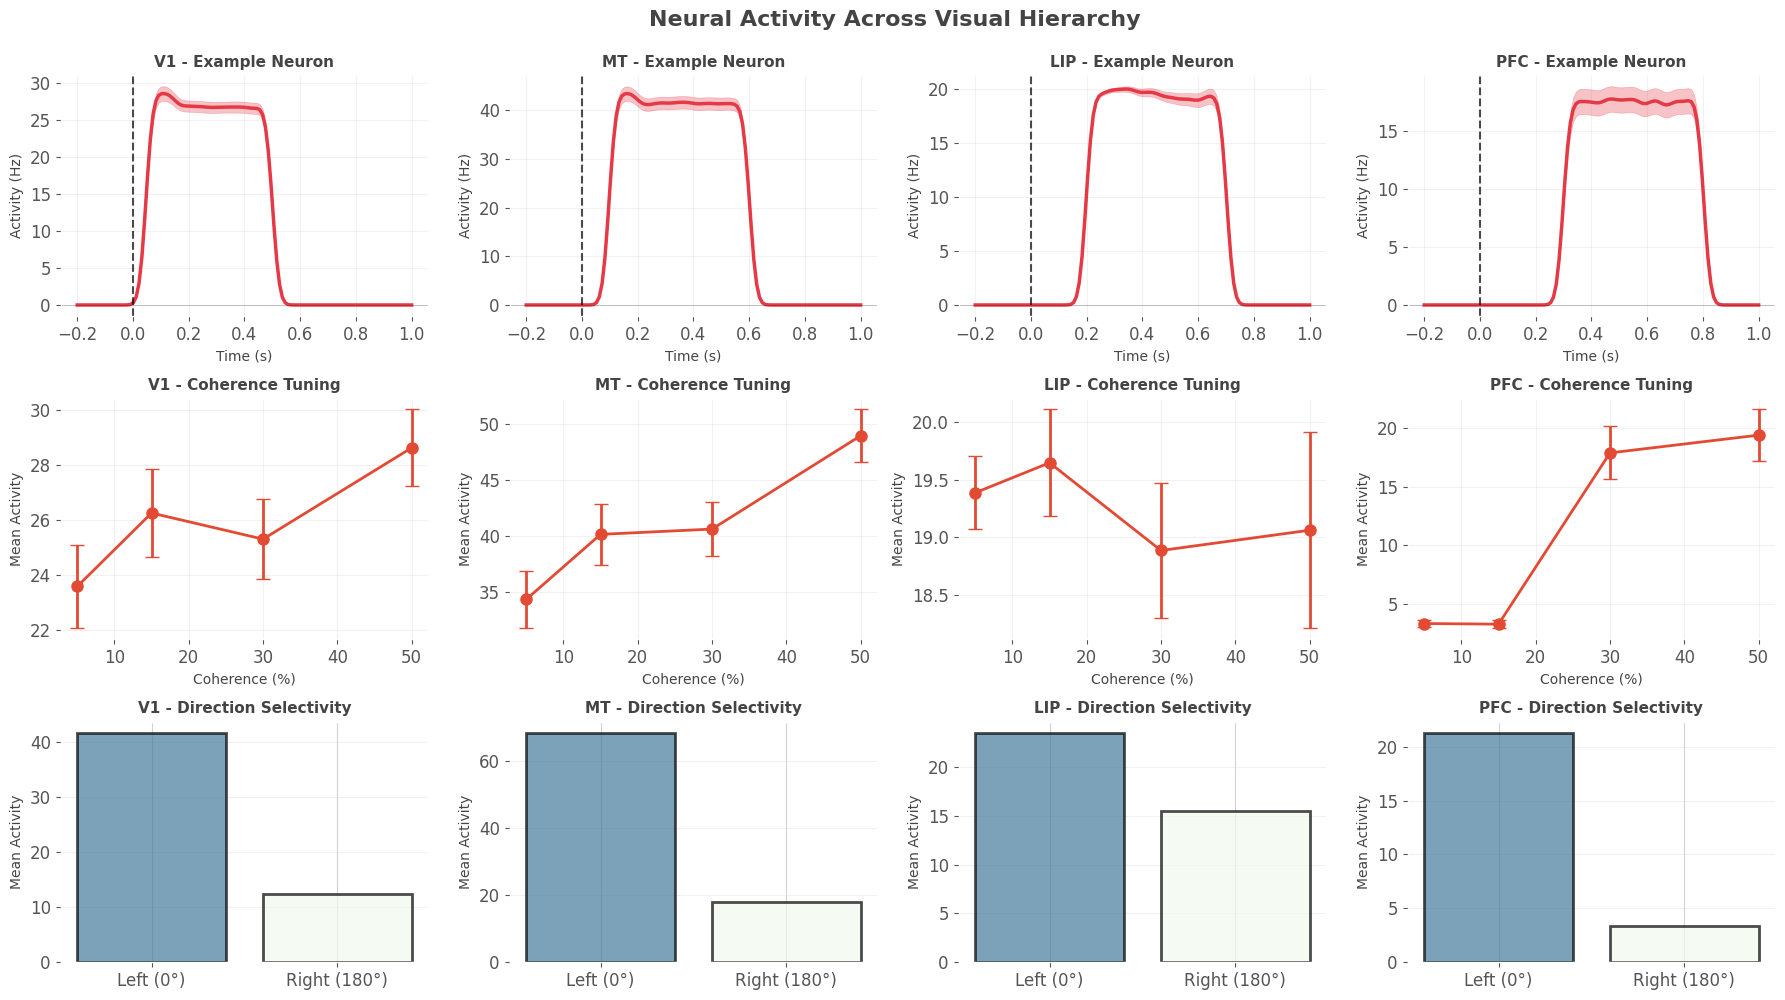
\includegraphics[keepaspectratio]{06_complete_integration_files/figure-pdf/cell-5-output-1.png}}

\begin{verbatim}

✓ Data visualization complete

💡 Key Observations:
   • V1: Early onset, modest coherence sensitivity
   • MT: Medium latency, strong coherence tuning
   • LIP: Late onset, ramping activity (accumulation)
   • PFC: Sustained late activity (decision maintenance)

✨ Realistic hierarchical dynamics for analysis!
\end{verbatim}

\section{Part 2: FRITES Analysis - Time-Resolved Information
Flow}\label{part-2-frites-analysis---time-resolved-information-flow}

\subsection{Question 1: When does coherence information emerge in each
area?}\label{question-1-when-does-coherence-information-emerge-in-each-area}

We'll use Frites to compute time-resolved mutual information between
neural activity and motion coherence. This reveals \textbf{when} each
brain area represents task-relevant information.

\begin{Shaded}
\begin{Highlighting}[]
\BuiltInTok{print}\NormalTok{(}\StringTok{"FRITES ANALYSIS: Time{-}Resolved Coherence Information"}\NormalTok{)}
\BuiltInTok{print}\NormalTok{(}\StringTok{"="} \OperatorTok{*} \DecValTok{70}\NormalTok{)}

\CommentTok{\# Convert to Frites format}
\NormalTok{data\_frites, coherence\_frites, direction\_frites, roi\_frites }\OperatorTok{=}\NormalTok{ sim.get\_frites\_format(n\_subjects}\OperatorTok{=}\DecValTok{5}\NormalTok{)}

\CommentTok{\# Create dataset}
\NormalTok{ds\_coherence }\OperatorTok{=}\NormalTok{ DatasetEphy(}
\NormalTok{    x}\OperatorTok{=}\NormalTok{data\_frites,}
\NormalTok{    y}\OperatorTok{=}\NormalTok{coherence\_frites,  }\CommentTok{\# Coherence as task variable}
\NormalTok{    roi}\OperatorTok{=}\NormalTok{roi\_frites,}
\NormalTok{    times}\OperatorTok{=}\NormalTok{sim.time}
\NormalTok{)}

\BuiltInTok{print}\NormalTok{(}\StringTok{"Computing time{-}resolved I(Neural; Coherence)..."}\NormalTok{)}
\BuiltInTok{print}\NormalTok{(}\StringTok{"This may take 1{-}2 minutes...}\CharTok{\textbackslash{}n}\StringTok{"}\NormalTok{)}

\CommentTok{\# Workflow}
\NormalTok{wf\_coherence }\OperatorTok{=}\NormalTok{ WfMi(mi\_type}\OperatorTok{=}\StringTok{\textquotesingle{}cc\textquotesingle{}}\NormalTok{, inference}\OperatorTok{=}\StringTok{\textquotesingle{}rfx\textquotesingle{}}\NormalTok{, verbose}\OperatorTok{=}\VariableTok{True}\NormalTok{)}

\CommentTok{\# Compute with robust but simpler multiple{-}comparisons correction}
\CommentTok{\# Note: some versions of Frites have issues with mcp=\textquotesingle{}cluster\textquotesingle{} + cluster\_th=\textquotesingle{}tfce\textquotesingle{}}
\CommentTok{\# leading to a NoneType error inside the cluster correction. Here we use}
\CommentTok{\# FDR{-}based correction instead, which is stable across versions.}
\NormalTok{mi\_coherence, pv\_coherence }\OperatorTok{=}\NormalTok{ wf\_coherence.fit(}
\NormalTok{    ds\_coherence,}
\NormalTok{    n\_perm}\OperatorTok{=}\DecValTok{500}\NormalTok{,  }\CommentTok{\# More permutations for final analysis}
\NormalTok{    mcp}\OperatorTok{=}\StringTok{\textquotesingle{}fdr\textquotesingle{}}\NormalTok{,   }\CommentTok{\# Use FDR instead of cluster{-}based correction}
\NormalTok{    random\_state}\OperatorTok{=}\DecValTok{42}\NormalTok{,}
\NormalTok{    n\_jobs}\OperatorTok{=}\DecValTok{1}
\NormalTok{)}

\BuiltInTok{print}\NormalTok{(}\StringTok{"}\CharTok{\textbackslash{}n}\StringTok{✓ Time{-}resolved MI computed with statistical testing!"}\NormalTok{)}
\end{Highlighting}
\end{Shaded}

\begin{verbatim}
FRITES ANALYSIS: Time-Resolved Coherence Information
======================================================================
Computing time-resolved I(Neural; Coherence)...
This may take 1-2 minutes...
\end{verbatim}

\begin{verbatim}

✓ Time-resolved MI computed with statistical testing!
\end{verbatim}

\begin{Shaded}
\begin{Highlighting}[]
\CommentTok{\# Step 2: HOI analysis to find synergistic triplets}
\BuiltInTok{print}\NormalTok{(}\StringTok{"}\CharTok{\textbackslash{}n}\StringTok{Step 2: HOI Analysis for Synergistic Triplets"}\NormalTok{)}
\BuiltInTok{print}\NormalTok{(}\StringTok{"="} \OperatorTok{*} \DecValTok{60}\NormalTok{)}

\ImportTok{from}\NormalTok{ hoi.metrics }\ImportTok{import}\NormalTok{ Oinfo}

\CommentTok{\# Use the simulated dataset from \textasciigrave{}sim\textasciigrave{}}
\CommentTok{\# Average activity across time so each trial is a sample and each neuron a feature}
\CommentTok{\# First average over time → (n\_neurons, n\_trials), then transpose for HOI → (n\_trials, n\_neurons)}
\NormalTok{responses\_hoi }\OperatorTok{=}\NormalTok{ sim.responses.mean(axis}\OperatorTok{=}\DecValTok{2}\NormalTok{).T}

\CommentTok{\# Scan all triplets across all neurons}
\NormalTok{all\_triplets }\OperatorTok{=} \BuiltInTok{list}\NormalTok{(combinations(}\BuiltInTok{range}\NormalTok{(sim.n\_neurons), }\DecValTok{3}\NormalTok{))}
\BuiltInTok{print}\NormalTok{(}\SpecialStringTok{f"Testing }\SpecialCharTok{\{}\BuiltInTok{len}\NormalTok{(all\_triplets)}\SpecialCharTok{\}}\SpecialStringTok{ triplets..."}\NormalTok{)}

\CommentTok{\# Create Oinfo model with this data and compute O{-}information for all triplets of size 3}
\NormalTok{model\_oinfo }\OperatorTok{=}\NormalTok{ Oinfo(responses\_hoi)}
\NormalTok{oinfo\_results }\OperatorTok{=}\NormalTok{ model\_oinfo.fit(method}\OperatorTok{=}\StringTok{\textquotesingle{}gc\textquotesingle{}}\NormalTok{, minsize}\OperatorTok{=}\DecValTok{3}\NormalTok{, maxsize}\OperatorTok{=}\DecValTok{3}\NormalTok{)}

\CommentTok{\# Find synergistic ones}
\NormalTok{synergy\_threshold }\OperatorTok{=} \OperatorTok{{-}}\FloatTok{0.05}
\CommentTok{\# oinfo\_results elements can be 0{-}dim numpy arrays; cast to float}
\NormalTok{synergistic }\OperatorTok{=}\NormalTok{ [}
\NormalTok{    (trip, }\BuiltInTok{float}\NormalTok{(oi))}
    \ControlFlowTok{for}\NormalTok{ trip, oi }\KeywordTok{in} \BuiltInTok{zip}\NormalTok{(all\_triplets, oinfo\_results)}
    \ControlFlowTok{if} \BuiltInTok{float}\NormalTok{(oi) }\OperatorTok{\textless{}}\NormalTok{ synergy\_threshold}
\NormalTok{]}
\NormalTok{synergistic.sort(key}\OperatorTok{=}\KeywordTok{lambda}\NormalTok{ x: x[}\DecValTok{1}\NormalTok{])}

\BuiltInTok{print}\NormalTok{(}\SpecialStringTok{f"}\CharTok{\textbackslash{}n}\SpecialStringTok{✓ Found }\SpecialCharTok{\{}\BuiltInTok{len}\NormalTok{(synergistic)}\SpecialCharTok{\}}\SpecialStringTok{ synergistic triplets"}\NormalTok{)}
\BuiltInTok{print}\NormalTok{(}\SpecialStringTok{f"}\CharTok{\textbackslash{}n}\SpecialStringTok{Top 3:"}\NormalTok{)}
\ControlFlowTok{for}\NormalTok{ i, (trip, oi) }\KeywordTok{in} \BuiltInTok{enumerate}\NormalTok{(synergistic[:}\DecValTok{3}\NormalTok{]):}
    \BuiltInTok{print}\NormalTok{(}\SpecialStringTok{f"  }\SpecialCharTok{\{}\NormalTok{i}\OperatorTok{+}\DecValTok{1}\SpecialCharTok{\}}\SpecialStringTok{. Neurons }\SpecialCharTok{\{}\NormalTok{trip}\SpecialCharTok{\}}\SpecialStringTok{: O{-}info = }\SpecialCharTok{\{}\NormalTok{oi}\SpecialCharTok{:.4f\}}\SpecialStringTok{ bits"}\NormalTok{)}
\end{Highlighting}
\end{Shaded}

\begin{verbatim}

Step 2: HOI Analysis for Synergistic Triplets
============================================================
Testing 220 triplets...
\end{verbatim}

\begin{verbatim}

✓ Found 8 synergistic triplets

Top 3:
  1. Neurons (5, 6, 10): O-info = -0.1237 bits
  2. Neurons (2, 6, 10): O-info = -0.1137 bits
  3. Neurons (2, 8, 10): O-info = -0.1018 bits
\end{verbatim}

\begin{Shaded}
\begin{Highlighting}[]
\CommentTok{\# Visualize results by brain area}
\NormalTok{fig, axes }\OperatorTok{=}\NormalTok{ plt.subplots(}\DecValTok{4}\NormalTok{, }\DecValTok{1}\NormalTok{, figsize}\OperatorTok{=}\NormalTok{(}\DecValTok{15}\NormalTok{, }\DecValTok{14}\NormalTok{), sharex}\OperatorTok{=}\VariableTok{True}\NormalTok{)}

\NormalTok{area\_colors }\OperatorTok{=}\NormalTok{ \{}\StringTok{\textquotesingle{}V1\textquotesingle{}}\NormalTok{: }\StringTok{\textquotesingle{}\#E63946\textquotesingle{}}\NormalTok{, }\StringTok{\textquotesingle{}MT\textquotesingle{}}\NormalTok{: }\StringTok{\textquotesingle{}\#457B9D\textquotesingle{}}\NormalTok{, }\StringTok{\textquotesingle{}LIP\textquotesingle{}}\NormalTok{: }\StringTok{\textquotesingle{}\#A8DADC\textquotesingle{}}\NormalTok{, }\StringTok{\textquotesingle{}PFC\textquotesingle{}}\NormalTok{: }\StringTok{\textquotesingle{}\#F1FAEE\textquotesingle{}}\NormalTok{\}}

\ControlFlowTok{for}\NormalTok{ area\_idx, area\_name }\KeywordTok{in} \BuiltInTok{enumerate}\NormalTok{(area\_names):}
\NormalTok{    ax }\OperatorTok{=}\NormalTok{ axes[area\_idx]}
    
    \CommentTok{\# Get neurons in this area}
\NormalTok{    area\_neurons }\OperatorTok{=}\NormalTok{ [roi }\ControlFlowTok{for}\NormalTok{ roi }\KeywordTok{in}\NormalTok{ roi\_frites[}\DecValTok{0}\NormalTok{] }\ControlFlowTok{if}\NormalTok{ area\_name }\KeywordTok{in}\NormalTok{ roi]}
    
    \CommentTok{\# Plot each neuron}
    \ControlFlowTok{for}\NormalTok{ neuron\_name }\KeywordTok{in}\NormalTok{ area\_neurons:}
\NormalTok{        mi\_neuron }\OperatorTok{=}\NormalTok{ mi\_coherence.sel(roi}\OperatorTok{=}\NormalTok{neuron\_name).squeeze()}
\NormalTok{        pv\_neuron }\OperatorTok{=}\NormalTok{ pv\_coherence.sel(roi}\OperatorTok{=}\NormalTok{neuron\_name).squeeze()}
        
        \CommentTok{\# Plot MI}
\NormalTok{        line }\OperatorTok{=}\NormalTok{ ax.plot(sim.time, mi\_neuron, linewidth}\OperatorTok{=}\DecValTok{2}\NormalTok{, }
\NormalTok{                      alpha}\OperatorTok{=}\FloatTok{0.7}\NormalTok{, label}\OperatorTok{=}\NormalTok{neuron\_name)[}\DecValTok{0}\NormalTok{]}
        
        \CommentTok{\# Highlight significant periods}
\NormalTok{        sig }\OperatorTok{=}\NormalTok{ pv\_neuron.values }\OperatorTok{\textless{}} \FloatTok{0.05}
        \ControlFlowTok{if}\NormalTok{ sig.}\BuiltInTok{any}\NormalTok{():}
\NormalTok{            ax.fill\_between(sim.time, }\DecValTok{0}\NormalTok{, mi\_neuron, where}\OperatorTok{=}\NormalTok{sig,}
\NormalTok{                          alpha}\OperatorTok{=}\FloatTok{0.2}\NormalTok{, color}\OperatorTok{=}\NormalTok{line.get\_color())}
    
    \CommentTok{\# Area mean}
\NormalTok{    area\_mi\_mean }\OperatorTok{=}\NormalTok{ np.mean([mi\_coherence.sel(roi}\OperatorTok{=}\NormalTok{n).squeeze().values }
                           \ControlFlowTok{for}\NormalTok{ n }\KeywordTok{in}\NormalTok{ area\_neurons], axis}\OperatorTok{=}\DecValTok{0}\NormalTok{)}
\NormalTok{    ax.plot(sim.time, area\_mi\_mean, linewidth}\OperatorTok{=}\DecValTok{4}\NormalTok{, color}\OperatorTok{=}\NormalTok{area\_colors[area\_name],}
\NormalTok{           label}\OperatorTok{=}\SpecialStringTok{f\textquotesingle{}}\SpecialCharTok{\{}\NormalTok{area\_name}\SpecialCharTok{\}}\SpecialStringTok{ mean\textquotesingle{}}\NormalTok{, alpha}\OperatorTok{=}\FloatTok{0.9}\NormalTok{, linestyle}\OperatorTok{=}\StringTok{\textquotesingle{}{-}{-}\textquotesingle{}}\NormalTok{)}
    
    \CommentTok{\# Formatting}
\NormalTok{    ax.axvline(}\DecValTok{0}\NormalTok{, color}\OperatorTok{=}\StringTok{\textquotesingle{}k\textquotesingle{}}\NormalTok{, linestyle}\OperatorTok{=}\StringTok{\textquotesingle{}{-}{-}\textquotesingle{}}\NormalTok{, linewidth}\OperatorTok{=}\DecValTok{2}\NormalTok{, alpha}\OperatorTok{=}\FloatTok{0.7}\NormalTok{, label}\OperatorTok{=}\StringTok{\textquotesingle{}Stimulus\textquotesingle{}}\NormalTok{)}
\NormalTok{    ax.axhline(}\DecValTok{0}\NormalTok{, color}\OperatorTok{=}\StringTok{\textquotesingle{}k\textquotesingle{}}\NormalTok{, linestyle}\OperatorTok{=}\StringTok{\textquotesingle{}{-}\textquotesingle{}}\NormalTok{, linewidth}\OperatorTok{=}\DecValTok{1}\NormalTok{, alpha}\OperatorTok{=}\FloatTok{0.3}\NormalTok{)}
\NormalTok{    ax.set\_ylabel(}\StringTok{\textquotesingle{}MI (bits)\textquotesingle{}}\NormalTok{, fontsize}\OperatorTok{=}\DecValTok{12}\NormalTok{, fontweight}\OperatorTok{=}\StringTok{\textquotesingle{}bold\textquotesingle{}}\NormalTok{)}
\NormalTok{    ax.set\_title(}\SpecialStringTok{f\textquotesingle{}}\SpecialCharTok{\{}\NormalTok{area\_name}\SpecialCharTok{\}}\SpecialStringTok{ {-} Coherence Information\textquotesingle{}}\NormalTok{, }
\NormalTok{                fontsize}\OperatorTok{=}\DecValTok{13}\NormalTok{, fontweight}\OperatorTok{=}\StringTok{\textquotesingle{}bold\textquotesingle{}}\NormalTok{, loc}\OperatorTok{=}\StringTok{\textquotesingle{}left\textquotesingle{}}\NormalTok{)}
\NormalTok{    ax.legend(loc}\OperatorTok{=}\StringTok{\textquotesingle{}upper right\textquotesingle{}}\NormalTok{, fontsize}\OperatorTok{=}\DecValTok{9}\NormalTok{, ncol}\OperatorTok{=}\DecValTok{2}\NormalTok{)}
\NormalTok{    ax.grid(}\VariableTok{True}\NormalTok{, alpha}\OperatorTok{=}\FloatTok{0.3}\NormalTok{)}
    
    \CommentTok{\# Find peak time}
\NormalTok{    peak\_time }\OperatorTok{=}\NormalTok{ sim.time[np.argmax(area\_mi\_mean)]}
\NormalTok{    peak\_mi }\OperatorTok{=}\NormalTok{ np.}\BuiltInTok{max}\NormalTok{(area\_mi\_mean)}
\NormalTok{    ax.text(}\FloatTok{0.02}\NormalTok{, }\FloatTok{0.95}\NormalTok{, }\SpecialStringTok{f\textquotesingle{}Peak: }\SpecialCharTok{\{}\NormalTok{peak\_mi}\SpecialCharTok{:.3f\}}\SpecialStringTok{ bits @ }\SpecialCharTok{\{}\NormalTok{peak\_time}\SpecialCharTok{:.2f\}}\SpecialStringTok{s\textquotesingle{}}\NormalTok{,}
\NormalTok{           transform}\OperatorTok{=}\NormalTok{ax.transAxes, fontsize}\OperatorTok{=}\DecValTok{10}\NormalTok{, fontweight}\OperatorTok{=}\StringTok{\textquotesingle{}bold\textquotesingle{}}\NormalTok{,}
\NormalTok{           bbox}\OperatorTok{=}\BuiltInTok{dict}\NormalTok{(boxstyle}\OperatorTok{=}\StringTok{\textquotesingle{}round\textquotesingle{}}\NormalTok{, facecolor}\OperatorTok{=}\StringTok{\textquotesingle{}yellow\textquotesingle{}}\NormalTok{, alpha}\OperatorTok{=}\FloatTok{0.7}\NormalTok{),}
\NormalTok{           verticalalignment}\OperatorTok{=}\StringTok{\textquotesingle{}top\textquotesingle{}}\NormalTok{)}

\NormalTok{axes[}\OperatorTok{{-}}\DecValTok{1}\NormalTok{].set\_xlabel(}\StringTok{\textquotesingle{}Time (s)\textquotesingle{}}\NormalTok{, fontsize}\OperatorTok{=}\DecValTok{13}\NormalTok{, fontweight}\OperatorTok{=}\StringTok{\textquotesingle{}bold\textquotesingle{}}\NormalTok{)}
\NormalTok{plt.suptitle(}\StringTok{\textquotesingle{}Hierarchical Information Flow: Coherence Encoding\textquotesingle{}}\NormalTok{, }
\NormalTok{             fontsize}\OperatorTok{=}\DecValTok{16}\NormalTok{, fontweight}\OperatorTok{=}\StringTok{\textquotesingle{}bold\textquotesingle{}}\NormalTok{, y}\OperatorTok{=}\FloatTok{0.995}\NormalTok{)}
\NormalTok{plt.tight\_layout()}
\NormalTok{plt.show()}

\CommentTok{\# Summary statistics}
\BuiltInTok{print}\NormalTok{(}\StringTok{"}\CharTok{\textbackslash{}n}\StringTok{📊 Information Onset Times (50}\SpecialCharTok{\% o}\StringTok{f peak):"}\NormalTok{)}
\BuiltInTok{print}\NormalTok{(}\StringTok{"="} \OperatorTok{*} \DecValTok{70}\NormalTok{)}
\ControlFlowTok{for}\NormalTok{ area\_name }\KeywordTok{in}\NormalTok{ area\_names:}
\NormalTok{    area\_neurons }\OperatorTok{=}\NormalTok{ [roi }\ControlFlowTok{for}\NormalTok{ roi }\KeywordTok{in}\NormalTok{ roi\_frites[}\DecValTok{0}\NormalTok{] }\ControlFlowTok{if}\NormalTok{ area\_name }\KeywordTok{in}\NormalTok{ roi]}
\NormalTok{    area\_mi }\OperatorTok{=}\NormalTok{ np.mean([mi\_coherence.sel(roi}\OperatorTok{=}\NormalTok{n).squeeze().values }
                      \ControlFlowTok{for}\NormalTok{ n }\KeywordTok{in}\NormalTok{ area\_neurons], axis}\OperatorTok{=}\DecValTok{0}\NormalTok{)}
    
\NormalTok{    peak\_mi }\OperatorTok{=}\NormalTok{ area\_mi.}\BuiltInTok{max}\NormalTok{()}
\NormalTok{    threshold }\OperatorTok{=}\NormalTok{ peak\_mi }\OperatorTok{*} \FloatTok{0.5}
\NormalTok{    above\_thresh }\OperatorTok{=}\NormalTok{ area\_mi }\OperatorTok{\textgreater{}}\NormalTok{ threshold}
    
    \ControlFlowTok{if}\NormalTok{ above\_thresh.}\BuiltInTok{any}\NormalTok{():}
\NormalTok{        onset\_idx }\OperatorTok{=}\NormalTok{ np.where(above\_thresh)[}\DecValTok{0}\NormalTok{][}\DecValTok{0}\NormalTok{]}
\NormalTok{        onset\_time }\OperatorTok{=}\NormalTok{ sim.time[onset\_idx]}
        \BuiltInTok{print}\NormalTok{(}\SpecialStringTok{f"}\SpecialCharTok{\{}\NormalTok{area\_name}\SpecialCharTok{:4s\}}\SpecialStringTok{: }\SpecialCharTok{\{}\NormalTok{onset\_time}\SpecialCharTok{:6.3f\}}\SpecialStringTok{s (peak: }\SpecialCharTok{\{}\NormalTok{peak\_mi}\SpecialCharTok{:.3f\}}\SpecialStringTok{ bits)"}\NormalTok{)}
    \ControlFlowTok{else}\NormalTok{:}
        \BuiltInTok{print}\NormalTok{(}\SpecialStringTok{f"}\SpecialCharTok{\{}\NormalTok{area\_name}\SpecialCharTok{:4s\}}\SpecialStringTok{: No significant information"}\NormalTok{)}

\BuiltInTok{print}\NormalTok{(}\StringTok{"}\CharTok{\textbackslash{}n}\StringTok{✨ Information flows hierarchically:"}\NormalTok{)}
\BuiltInTok{print}\NormalTok{(}\StringTok{"   V1 → MT → LIP → PFC"}\NormalTok{)}
\BuiltInTok{print}\NormalTok{(}\StringTok{"   Early sensory → Late decision"}\NormalTok{)}
\end{Highlighting}
\end{Shaded}

\pandocbounded{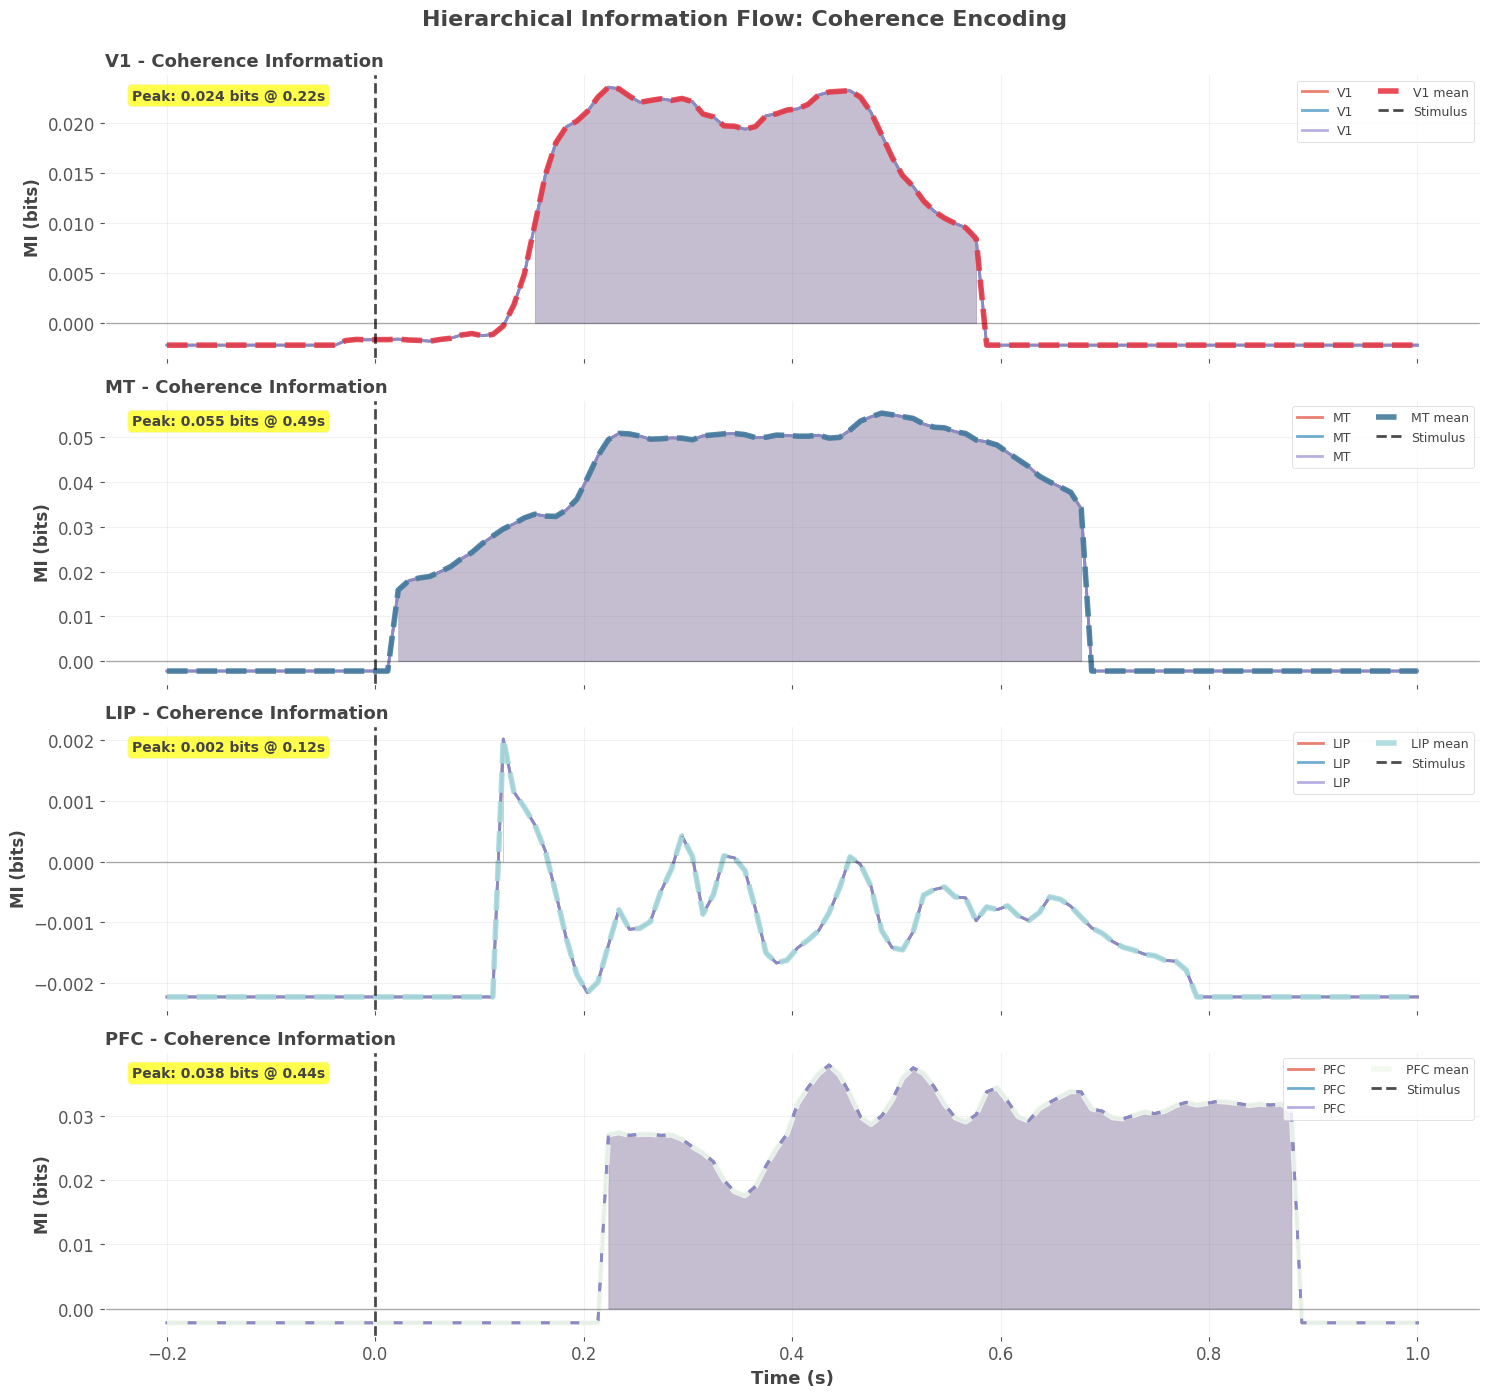
\includegraphics[keepaspectratio]{06_complete_integration_files/figure-pdf/cell-8-output-1.png}}

\begin{verbatim}

📊 Information Onset Times (50% of peak):
======================================================================
V1  :  0.163s (peak: 0.024 bits)
MT  :  0.113s (peak: 0.055 bits)
LIP :  0.123s (peak: 0.002 bits)
PFC :  0.224s (peak: 0.038 bits)

✨ Information flows hierarchically:
   V1 → MT → LIP → PFC
   Early sensory → Late decision
\end{verbatim}

\section{Part 3: HOI Analysis - Discovering Synergistic
Ensembles}\label{part-3-hoi-analysis---discovering-synergistic-ensembles}

\subsection{Question 2: Which neuron triplets show synergistic
coding?}\label{question-2-which-neuron-triplets-show-synergistic-coding}

Now we'll use HOI to scan for synergistic interactions. We'll focus on
the \textbf{decision period} (200-600ms) where we expect rich
interactions.

\begin{Shaded}
\begin{Highlighting}[]
\BuiltInTok{print}\NormalTok{(}\StringTok{"HOI ANALYSIS: Synergistic Ensemble Detection"}\NormalTok{)}
\BuiltInTok{print}\NormalTok{(}\StringTok{"="} \OperatorTok{*} \DecValTok{70}\NormalTok{)}

\CommentTok{\# Extract decision period data}
\NormalTok{decision\_window }\OperatorTok{=}\NormalTok{ (sim.time }\OperatorTok{\textgreater{}=} \FloatTok{0.2}\NormalTok{) }\OperatorTok{\&}\NormalTok{ (sim.time }\OperatorTok{\textless{}=} \FloatTok{0.6}\NormalTok{)}

\CommentTok{\# Average neural activity in this window}
\CommentTok{\# Shape after mean: (n\_neurons, n\_trials)}
\CommentTok{\# We need to TRANSPOSE for HOI: (n\_samples, n\_features) = (n\_trials, n\_neurons)}
\NormalTok{activity\_decision }\OperatorTok{=}\NormalTok{ sim.responses[:, :, decision\_window].mean(axis}\OperatorTok{=}\DecValTok{2}\NormalTok{).T  }\CommentTok{\# Now (n\_trials, n\_neurons)}

\BuiltInTok{print}\NormalTok{(}\SpecialStringTok{f"Extracted decision period activity:"}\NormalTok{)}
\BuiltInTok{print}\NormalTok{(}\SpecialStringTok{f"  Shape: }\SpecialCharTok{\{}\NormalTok{activity\_decision}\SpecialCharTok{.}\NormalTok{shape}\SpecialCharTok{\}}\SpecialStringTok{"}\NormalTok{)}
\BuiltInTok{print}\NormalTok{(}\SpecialStringTok{f"  (trials × neurons) {-} correct format for HOI!"}\NormalTok{)}
\BuiltInTok{print}\NormalTok{(}\SpecialStringTok{f"}\CharTok{\textbackslash{}n}\SpecialStringTok{Scanning all possible triplets..."}\NormalTok{)}

\CommentTok{\# Scan all triplets}
\NormalTok{all\_triplets }\OperatorTok{=} \BuiltInTok{list}\NormalTok{(combinations(}\BuiltInTok{range}\NormalTok{(sim.n\_neurons), }\DecValTok{3}\NormalTok{))}
\BuiltInTok{print}\NormalTok{(}\SpecialStringTok{f"  Total triplets to test: }\SpecialCharTok{\{}\BuiltInTok{len}\NormalTok{(all\_triplets)}\SpecialCharTok{\}}\SpecialStringTok{"}\NormalTok{)}

\CommentTok{\# Compute O{-}information}
\CommentTok{\# Create model with data in constructor}
\NormalTok{model\_oinfo }\OperatorTok{=}\NormalTok{ Oinfo(activity\_decision)}
\NormalTok{oinfo\_values }\OperatorTok{=}\NormalTok{ model\_oinfo.fit(method}\OperatorTok{=}\StringTok{"gc"}\NormalTok{, minsize}\OperatorTok{=}\DecValTok{3}\NormalTok{, maxsize}\OperatorTok{=}\DecValTok{3}\NormalTok{)}

\BuiltInTok{print}\NormalTok{(}\SpecialStringTok{f"}\CharTok{\textbackslash{}n}\SpecialStringTok{✓ O{-}information computed for all triplets"}\NormalTok{)}

\CommentTok{\# Categorize by synergy/redundancy}
\NormalTok{synergy\_threshold }\OperatorTok{=} \OperatorTok{{-}}\FloatTok{0.05}
\NormalTok{redundancy\_threshold }\OperatorTok{=} \FloatTok{0.05}

\CommentTok{\# Convert oinfo\_values to list of floats for easier handling}
\NormalTok{oinfo\_list }\OperatorTok{=}\NormalTok{ [}\BuiltInTok{float}\NormalTok{(v) }\ControlFlowTok{for}\NormalTok{ v }\KeywordTok{in}\NormalTok{ oinfo\_values]}

\NormalTok{synergistic }\OperatorTok{=}\NormalTok{ [(trip, oi) }\ControlFlowTok{for}\NormalTok{ trip, oi }\KeywordTok{in} \BuiltInTok{zip}\NormalTok{(all\_triplets, oinfo\_list) }
               \ControlFlowTok{if}\NormalTok{ oi }\OperatorTok{\textless{}}\NormalTok{ synergy\_threshold]}
\NormalTok{redundant }\OperatorTok{=}\NormalTok{ [(trip, oi) }\ControlFlowTok{for}\NormalTok{ trip, oi }\KeywordTok{in} \BuiltInTok{zip}\NormalTok{(all\_triplets, oinfo\_list)}
            \ControlFlowTok{if}\NormalTok{ oi }\OperatorTok{\textgreater{}}\NormalTok{ redundancy\_threshold]}
\NormalTok{independent }\OperatorTok{=}\NormalTok{ [(trip, oi) }\ControlFlowTok{for}\NormalTok{ trip, oi }\KeywordTok{in} \BuiltInTok{zip}\NormalTok{(all\_triplets, oinfo\_list)}
              \ControlFlowTok{if} \BuiltInTok{abs}\NormalTok{(oi) }\OperatorTok{\textless{}=} \BuiltInTok{max}\NormalTok{(}\BuiltInTok{abs}\NormalTok{(synergy\_threshold), redundancy\_threshold)]}

\NormalTok{synergistic.sort(key}\OperatorTok{=}\KeywordTok{lambda}\NormalTok{ x: x[}\DecValTok{1}\NormalTok{])  }\CommentTok{\# Most negative first}
\NormalTok{redundant.sort(key}\OperatorTok{=}\KeywordTok{lambda}\NormalTok{ x: x[}\DecValTok{1}\NormalTok{], reverse}\OperatorTok{=}\VariableTok{True}\NormalTok{)  }\CommentTok{\# Most positive first}

\BuiltInTok{print}\NormalTok{(}\SpecialStringTok{f"}\CharTok{\textbackslash{}n}\SpecialStringTok{📊 O{-}Information Results:"}\NormalTok{)}
\BuiltInTok{print}\NormalTok{(}\StringTok{"="} \OperatorTok{*} \DecValTok{70}\NormalTok{)}
\BuiltInTok{print}\NormalTok{(}\SpecialStringTok{f"Total triplets: }\SpecialCharTok{\{}\BuiltInTok{len}\NormalTok{(all\_triplets)}\SpecialCharTok{\}}\SpecialStringTok{"}\NormalTok{)}
\BuiltInTok{print}\NormalTok{(}\SpecialStringTok{f"  Synergistic (O \textless{} }\SpecialCharTok{\{}\NormalTok{synergy\_threshold}\SpecialCharTok{\}}\SpecialStringTok{): }\SpecialCharTok{\{}\BuiltInTok{len}\NormalTok{(synergistic)}\SpecialCharTok{\}}\SpecialStringTok{ (}\SpecialCharTok{\{}\BuiltInTok{len}\NormalTok{(synergistic)}\OperatorTok{/}\BuiltInTok{len}\NormalTok{(all\_triplets)}\OperatorTok{*}\DecValTok{100}\SpecialCharTok{:.1f\}}\SpecialStringTok{\%)"}\NormalTok{)}
\BuiltInTok{print}\NormalTok{(}\SpecialStringTok{f"  Independent (|O| ≤ }\SpecialCharTok{\{}\BuiltInTok{abs}\NormalTok{(synergy\_threshold)}\SpecialCharTok{\}}\SpecialStringTok{): }\SpecialCharTok{\{}\BuiltInTok{len}\NormalTok{(independent)}\SpecialCharTok{\}}\SpecialStringTok{ (}\SpecialCharTok{\{}\BuiltInTok{len}\NormalTok{(independent)}\OperatorTok{/}\BuiltInTok{len}\NormalTok{(all\_triplets)}\OperatorTok{*}\DecValTok{100}\SpecialCharTok{:.1f\}}\SpecialStringTok{\%)"}\NormalTok{)}
\BuiltInTok{print}\NormalTok{(}\SpecialStringTok{f"  Redundant (O \textgreater{} }\SpecialCharTok{\{}\NormalTok{redundancy\_threshold}\SpecialCharTok{\}}\SpecialStringTok{): }\SpecialCharTok{\{}\BuiltInTok{len}\NormalTok{(redundant)}\SpecialCharTok{\}}\SpecialStringTok{ (}\SpecialCharTok{\{}\BuiltInTok{len}\NormalTok{(redundant)}\OperatorTok{/}\BuiltInTok{len}\NormalTok{(all\_triplets)}\OperatorTok{*}\DecValTok{100}\SpecialCharTok{:.1f\}}\SpecialStringTok{\%)"}\NormalTok{)}

\CommentTok{\# Analyze synergistic triplets by area composition}
\BuiltInTok{print}\NormalTok{(}\SpecialStringTok{f"}\CharTok{\textbackslash{}n}\SpecialStringTok{🔍 Top 10 Synergistic Triplets:"}\NormalTok{)}
\BuiltInTok{print}\NormalTok{(}\StringTok{"="} \OperatorTok{*} \DecValTok{70}\NormalTok{)}
\BuiltInTok{print}\NormalTok{(}\SpecialStringTok{f"}\SpecialCharTok{\{}\StringTok{\textquotesingle{}Rank\textquotesingle{}}\SpecialCharTok{:\textless{}6\}}\SpecialStringTok{ }\SpecialCharTok{\{}\StringTok{\textquotesingle{}Neurons\textquotesingle{}}\SpecialCharTok{:\textless{}15\}}\SpecialStringTok{ }\SpecialCharTok{\{}\StringTok{\textquotesingle{}Areas\textquotesingle{}}\SpecialCharTok{:\textless{}25\}}\SpecialStringTok{ }\SpecialCharTok{\{}\StringTok{\textquotesingle{}O{-}info\textquotesingle{}}\SpecialCharTok{:\textless{}12\}}\SpecialStringTok{"}\NormalTok{)}
\BuiltInTok{print}\NormalTok{(}\StringTok{"="} \OperatorTok{*} \DecValTok{70}\NormalTok{)}

\ControlFlowTok{for}\NormalTok{ rank, (triplet, oinfo) }\KeywordTok{in} \BuiltInTok{enumerate}\NormalTok{(synergistic[:}\DecValTok{10}\NormalTok{], }\DecValTok{1}\NormalTok{):}
\NormalTok{    neuron\_ids }\OperatorTok{=} \BuiltInTok{list}\NormalTok{(triplet)}
\NormalTok{    area\_composition }\OperatorTok{=}\NormalTok{ [sim.areas[n] }\ControlFlowTok{for}\NormalTok{ n }\KeywordTok{in}\NormalTok{ neuron\_ids]}
\NormalTok{    area\_str }\OperatorTok{=} \SpecialStringTok{f"}\SpecialCharTok{\{}\NormalTok{area\_composition[}\DecValTok{0}\NormalTok{]}\SpecialCharTok{\}}\SpecialStringTok{{-}}\SpecialCharTok{\{}\NormalTok{area\_composition[}\DecValTok{1}\NormalTok{]}\SpecialCharTok{\}}\SpecialStringTok{{-}}\SpecialCharTok{\{}\NormalTok{area\_composition[}\DecValTok{2}\NormalTok{]}\SpecialCharTok{\}}\SpecialStringTok{"}
    \BuiltInTok{print}\NormalTok{(}\SpecialStringTok{f"}\SpecialCharTok{\{}\NormalTok{rank}\SpecialCharTok{:\textless{}6\}}\SpecialStringTok{ }\SpecialCharTok{\{}\BuiltInTok{str}\NormalTok{(neuron\_ids)}\SpecialCharTok{:\textless{}15\}}\SpecialStringTok{ }\SpecialCharTok{\{}\NormalTok{area\_str}\SpecialCharTok{:\textless{}25\}}\SpecialStringTok{ }\SpecialCharTok{\{}\NormalTok{oinfo}\SpecialCharTok{:\textgreater{}10.4f\}}\SpecialStringTok{ bits"}\NormalTok{)}

\CommentTok{\# Classify triplets by area composition}
\NormalTok{within\_area }\OperatorTok{=} \DecValTok{0}
\NormalTok{cross\_area }\OperatorTok{=} \DecValTok{0}

\ControlFlowTok{for}\NormalTok{ triplet, \_ }\KeywordTok{in}\NormalTok{ synergistic:}
\NormalTok{    areas\_in\_triplet }\OperatorTok{=} \BuiltInTok{set}\NormalTok{([sim.areas[n] }\ControlFlowTok{for}\NormalTok{ n }\KeywordTok{in}\NormalTok{ triplet])}
    \ControlFlowTok{if} \BuiltInTok{len}\NormalTok{(areas\_in\_triplet) }\OperatorTok{==} \DecValTok{1}\NormalTok{:}
\NormalTok{        within\_area }\OperatorTok{+=} \DecValTok{1}
    \ControlFlowTok{else}\NormalTok{:}
\NormalTok{        cross\_area }\OperatorTok{+=} \DecValTok{1}

\BuiltInTok{print}\NormalTok{(}\SpecialStringTok{f"}\CharTok{\textbackslash{}n}\SpecialStringTok{📈 Area Composition of Synergistic Triplets:"}\NormalTok{)}
\BuiltInTok{print}\NormalTok{(}\SpecialStringTok{f"  Within{-}area: }\SpecialCharTok{\{}\NormalTok{within\_area}\SpecialCharTok{\}}\SpecialStringTok{ (}\SpecialCharTok{\{}\NormalTok{within\_area}\OperatorTok{/}\BuiltInTok{max}\NormalTok{(}\DecValTok{1}\NormalTok{,}\BuiltInTok{len}\NormalTok{(synergistic))}\OperatorTok{*}\DecValTok{100}\SpecialCharTok{:.1f\}}\SpecialStringTok{\%)"}\NormalTok{)}
\BuiltInTok{print}\NormalTok{(}\SpecialStringTok{f"  Cross{-}area: }\SpecialCharTok{\{}\NormalTok{cross\_area}\SpecialCharTok{\}}\SpecialStringTok{ (}\SpecialCharTok{\{}\NormalTok{cross\_area}\OperatorTok{/}\BuiltInTok{max}\NormalTok{(}\DecValTok{1}\NormalTok{,}\BuiltInTok{len}\NormalTok{(synergistic))}\OperatorTok{*}\DecValTok{100}\SpecialCharTok{:.1f\}}\SpecialStringTok{\%)"}\NormalTok{)}
\end{Highlighting}
\end{Shaded}

\begin{verbatim}
HOI ANALYSIS: Synergistic Ensemble Detection
======================================================================
Extracted decision period activity:
  Shape: (400, 12)
  (trials × neurons) - correct format for HOI!

Scanning all possible triplets...
  Total triplets to test: 220
\end{verbatim}

\begin{verbatim}

✓ O-information computed for all triplets

📊 O-Information Results:
======================================================================
Total triplets: 220
  Synergistic (O < -0.05): 7 (3.2%)
  Independent (|O| ≤ 0.05): 44 (20.0%)
  Redundant (O > 0.05): 169 (76.8%)

🔍 Top 10 Synergistic Triplets:
======================================================================
Rank   Neurons         Areas                     O-info      
======================================================================
1      [5, 6, 10]      MT-LIP-PFC                   -0.0875 bits
2      [2, 6, 10]      V1-LIP-PFC                   -0.0822 bits
3      [2, 8, 10]      V1-LIP-PFC                   -0.0675 bits
4      [5, 8, 10]      MT-LIP-PFC                   -0.0663 bits
5      [5, 6, 9]       MT-LIP-PFC                   -0.0619 bits
6      [5, 7, 10]      MT-LIP-PFC                   -0.0573 bits
7      [2, 7, 10]      V1-LIP-PFC                   -0.0540 bits

📈 Area Composition of Synergistic Triplets:
  Within-area: 0 (0.0%)
  Cross-area: 7 (100.0%)
\end{verbatim}

\subsection{Visualizing O-Information
Landscape}\label{visualizing-o-information-landscape}

\begin{Shaded}
\begin{Highlighting}[]
\CommentTok{\# Create comprehensive O{-}info visualization}
\NormalTok{fig, axes }\OperatorTok{=}\NormalTok{ plt.subplots(}\DecValTok{2}\NormalTok{, }\DecValTok{2}\NormalTok{, figsize}\OperatorTok{=}\NormalTok{(}\DecValTok{16}\NormalTok{, }\DecValTok{12}\NormalTok{))}

\CommentTok{\# Panel 1: O{-}info distribution}
\NormalTok{ax1 }\OperatorTok{=}\NormalTok{ axes[}\DecValTok{0}\NormalTok{, }\DecValTok{0}\NormalTok{]}
\NormalTok{ax1.hist(oinfo\_values, bins}\OperatorTok{=}\DecValTok{40}\NormalTok{, color}\OperatorTok{=}\StringTok{\textquotesingle{}purple\textquotesingle{}}\NormalTok{, alpha}\OperatorTok{=}\FloatTok{0.6}\NormalTok{, edgecolor}\OperatorTok{=}\StringTok{\textquotesingle{}black\textquotesingle{}}\NormalTok{)}
\NormalTok{ax1.axvline(}\DecValTok{0}\NormalTok{, color}\OperatorTok{=}\StringTok{\textquotesingle{}k\textquotesingle{}}\NormalTok{, linestyle}\OperatorTok{=}\StringTok{\textquotesingle{}{-}{-}\textquotesingle{}}\NormalTok{, linewidth}\OperatorTok{=}\DecValTok{2}\NormalTok{, label}\OperatorTok{=}\StringTok{\textquotesingle{}Zero\textquotesingle{}}\NormalTok{)}
\NormalTok{ax1.axvline(synergy\_threshold, color}\OperatorTok{=}\StringTok{\textquotesingle{}red\textquotesingle{}}\NormalTok{, linestyle}\OperatorTok{=}\StringTok{\textquotesingle{}:\textquotesingle{}}\NormalTok{, linewidth}\OperatorTok{=}\DecValTok{2}\NormalTok{,}
\NormalTok{           label}\OperatorTok{=}\SpecialStringTok{f\textquotesingle{}Synergy threshold (}\SpecialCharTok{\{}\NormalTok{synergy\_threshold}\SpecialCharTok{\}}\SpecialStringTok{)\textquotesingle{}}\NormalTok{)}
\NormalTok{ax1.axvline(redundancy\_threshold, color}\OperatorTok{=}\StringTok{\textquotesingle{}blue\textquotesingle{}}\NormalTok{, linestyle}\OperatorTok{=}\StringTok{\textquotesingle{}:\textquotesingle{}}\NormalTok{, linewidth}\OperatorTok{=}\DecValTok{2}\NormalTok{,}
\NormalTok{           label}\OperatorTok{=}\SpecialStringTok{f\textquotesingle{}Redundancy threshold (}\SpecialCharTok{\{}\NormalTok{redundancy\_threshold}\SpecialCharTok{\}}\SpecialStringTok{)\textquotesingle{}}\NormalTok{)}
\NormalTok{ax1.set\_xlabel(}\StringTok{\textquotesingle{}O{-}information (bits)\textquotesingle{}}\NormalTok{, fontsize}\OperatorTok{=}\DecValTok{12}\NormalTok{, fontweight}\OperatorTok{=}\StringTok{\textquotesingle{}bold\textquotesingle{}}\NormalTok{)}
\NormalTok{ax1.set\_ylabel(}\StringTok{\textquotesingle{}Count\textquotesingle{}}\NormalTok{, fontsize}\OperatorTok{=}\DecValTok{12}\NormalTok{, fontweight}\OperatorTok{=}\StringTok{\textquotesingle{}bold\textquotesingle{}}\NormalTok{)}
\NormalTok{ax1.set\_title(}\StringTok{\textquotesingle{}Distribution of O{-}Information Values\textquotesingle{}}\NormalTok{, fontsize}\OperatorTok{=}\DecValTok{13}\NormalTok{, fontweight}\OperatorTok{=}\StringTok{\textquotesingle{}bold\textquotesingle{}}\NormalTok{)}
\NormalTok{ax1.legend(fontsize}\OperatorTok{=}\DecValTok{10}\NormalTok{)}
\NormalTok{ax1.grid(}\VariableTok{True}\NormalTok{, alpha}\OperatorTok{=}\FloatTok{0.3}\NormalTok{)}

\CommentTok{\# Panel 2: Category pie chart}
\NormalTok{ax2 }\OperatorTok{=}\NormalTok{ axes[}\DecValTok{0}\NormalTok{, }\DecValTok{1}\NormalTok{]}
\NormalTok{categories }\OperatorTok{=}\NormalTok{ [}\StringTok{\textquotesingle{}Synergistic\textquotesingle{}}\NormalTok{, }\StringTok{\textquotesingle{}Independent\textquotesingle{}}\NormalTok{, }\StringTok{\textquotesingle{}Redundant\textquotesingle{}}\NormalTok{]}
\NormalTok{counts }\OperatorTok{=}\NormalTok{ [}\BuiltInTok{len}\NormalTok{(synergistic), }\BuiltInTok{len}\NormalTok{(independent), }\BuiltInTok{len}\NormalTok{(redundant)]}
\NormalTok{colors\_pie }\OperatorTok{=}\NormalTok{ [}\StringTok{\textquotesingle{}red\textquotesingle{}}\NormalTok{, }\StringTok{\textquotesingle{}gray\textquotesingle{}}\NormalTok{, }\StringTok{\textquotesingle{}blue\textquotesingle{}}\NormalTok{]}
\NormalTok{ax2.pie(counts, labels}\OperatorTok{=}\NormalTok{categories, colors}\OperatorTok{=}\NormalTok{colors\_pie, autopct}\OperatorTok{=}\StringTok{\textquotesingle{}}\SpecialCharTok{\%1.1f\%\%}\StringTok{\textquotesingle{}}\NormalTok{,}
\NormalTok{       startangle}\OperatorTok{=}\DecValTok{90}\NormalTok{, textprops}\OperatorTok{=}\NormalTok{\{}\StringTok{\textquotesingle{}fontsize\textquotesingle{}}\NormalTok{: }\DecValTok{12}\NormalTok{, }\StringTok{\textquotesingle{}fontweight\textquotesingle{}}\NormalTok{: }\StringTok{\textquotesingle{}bold\textquotesingle{}}\NormalTok{\})}
\NormalTok{ax2.set\_title(}\StringTok{\textquotesingle{}Information Structure}\CharTok{\textbackslash{}n}\StringTok{of Decision Network\textquotesingle{}}\NormalTok{, }
\NormalTok{             fontsize}\OperatorTok{=}\DecValTok{13}\NormalTok{, fontweight}\OperatorTok{=}\StringTok{\textquotesingle{}bold\textquotesingle{}}\NormalTok{)}

\CommentTok{\# Panel 3: Synergy strength by area composition}
\NormalTok{ax3 }\OperatorTok{=}\NormalTok{ axes[}\DecValTok{1}\NormalTok{, }\DecValTok{0}\NormalTok{]}
\NormalTok{area\_pairs }\OperatorTok{=}\NormalTok{ [}\StringTok{\textquotesingle{}V1{-}V1{-}V1\textquotesingle{}}\NormalTok{, }\StringTok{\textquotesingle{}MT{-}MT{-}MT\textquotesingle{}}\NormalTok{, }\StringTok{\textquotesingle{}LIP{-}LIP{-}LIP\textquotesingle{}}\NormalTok{, }\StringTok{\textquotesingle{}PFC{-}PFC{-}PFC\textquotesingle{}}\NormalTok{,}
             \StringTok{\textquotesingle{}V1{-}MT{-}LIP\textquotesingle{}}\NormalTok{, }\StringTok{\textquotesingle{}MT{-}LIP{-}PFC\textquotesingle{}}\NormalTok{, }\StringTok{\textquotesingle{}Mixed\textquotesingle{}}\NormalTok{]}
\NormalTok{synergy\_by\_composition }\OperatorTok{=}\NormalTok{ \{ap: [] }\ControlFlowTok{for}\NormalTok{ ap }\KeywordTok{in}\NormalTok{ area\_pairs\}}

\ControlFlowTok{for}\NormalTok{ triplet, oinfo }\KeywordTok{in}\NormalTok{ synergistic:}
\NormalTok{    areas }\OperatorTok{=}\NormalTok{ [sim.areas[n] }\ControlFlowTok{for}\NormalTok{ n }\KeywordTok{in}\NormalTok{ triplet]}
\NormalTok{    unique\_areas }\OperatorTok{=} \BuiltInTok{set}\NormalTok{(areas)}
    
    \ControlFlowTok{if} \BuiltInTok{len}\NormalTok{(unique\_areas) }\OperatorTok{==} \DecValTok{1}\NormalTok{:}
        \CommentTok{\# Within{-}area}
\NormalTok{        comp\_name }\OperatorTok{=} \SpecialStringTok{f"}\SpecialCharTok{\{}\NormalTok{areas[}\DecValTok{0}\NormalTok{]}\SpecialCharTok{\}}\SpecialStringTok{{-}}\SpecialCharTok{\{}\NormalTok{areas[}\DecValTok{0}\NormalTok{]}\SpecialCharTok{\}}\SpecialStringTok{{-}}\SpecialCharTok{\{}\NormalTok{areas[}\DecValTok{0}\NormalTok{]}\SpecialCharTok{\}}\SpecialStringTok{"}
        \ControlFlowTok{if}\NormalTok{ comp\_name }\KeywordTok{in}\NormalTok{ synergy\_by\_composition:}
\NormalTok{            synergy\_by\_composition[comp\_name].append(}\BuiltInTok{abs}\NormalTok{(oinfo))}
    \ControlFlowTok{elif} \BuiltInTok{len}\NormalTok{(unique\_areas) }\OperatorTok{==} \DecValTok{3}\NormalTok{:}
        \CommentTok{\# Specific hierarchical triplet}
\NormalTok{        sorted\_areas }\OperatorTok{=} \BuiltInTok{sorted}\NormalTok{(areas)}
\NormalTok{        comp\_name }\OperatorTok{=} \SpecialStringTok{f"}\SpecialCharTok{\{}\NormalTok{sorted\_areas[}\DecValTok{0}\NormalTok{]}\SpecialCharTok{\}}\SpecialStringTok{{-}}\SpecialCharTok{\{}\NormalTok{sorted\_areas[}\DecValTok{1}\NormalTok{]}\SpecialCharTok{\}}\SpecialStringTok{{-}}\SpecialCharTok{\{}\NormalTok{sorted\_areas[}\DecValTok{2}\NormalTok{]}\SpecialCharTok{\}}\SpecialStringTok{"}
        \ControlFlowTok{if}\NormalTok{ comp\_name }\KeywordTok{in}\NormalTok{ synergy\_by\_composition:}
\NormalTok{            synergy\_by\_composition[comp\_name].append(}\BuiltInTok{abs}\NormalTok{(oinfo))}
        \ControlFlowTok{else}\NormalTok{:}
\NormalTok{            synergy\_by\_composition[}\StringTok{\textquotesingle{}Mixed\textquotesingle{}}\NormalTok{].append(}\BuiltInTok{abs}\NormalTok{(oinfo))}
    \ControlFlowTok{else}\NormalTok{:}
\NormalTok{        synergy\_by\_composition[}\StringTok{\textquotesingle{}Mixed\textquotesingle{}}\NormalTok{].append(}\BuiltInTok{abs}\NormalTok{(oinfo))}

\CommentTok{\# Plot means}
\NormalTok{compositions\_present }\OperatorTok{=}\NormalTok{ [k }\ControlFlowTok{for}\NormalTok{ k, v }\KeywordTok{in}\NormalTok{ synergy\_by\_composition.items() }\ControlFlowTok{if} \BuiltInTok{len}\NormalTok{(v) }\OperatorTok{\textgreater{}} \DecValTok{0}\NormalTok{]}
\NormalTok{mean\_synergies }\OperatorTok{=}\NormalTok{ [np.mean(synergy\_by\_composition[k]) }\ControlFlowTok{for}\NormalTok{ k }\KeywordTok{in}\NormalTok{ compositions\_present]}
\NormalTok{count\_synergies }\OperatorTok{=}\NormalTok{ [}\BuiltInTok{len}\NormalTok{(synergy\_by\_composition[k]) }\ControlFlowTok{for}\NormalTok{ k }\KeywordTok{in}\NormalTok{ compositions\_present]}

\NormalTok{bars }\OperatorTok{=}\NormalTok{ ax3.bar(}\BuiltInTok{range}\NormalTok{(}\BuiltInTok{len}\NormalTok{(compositions\_present)), mean\_synergies, }
\NormalTok{              color}\OperatorTok{=}\StringTok{\textquotesingle{}\#E63946\textquotesingle{}}\NormalTok{, alpha}\OperatorTok{=}\FloatTok{0.7}\NormalTok{, edgecolor}\OperatorTok{=}\StringTok{\textquotesingle{}black\textquotesingle{}}\NormalTok{, linewidth}\OperatorTok{=}\FloatTok{1.5}\NormalTok{)}
\NormalTok{ax3.set\_xticks(}\BuiltInTok{range}\NormalTok{(}\BuiltInTok{len}\NormalTok{(compositions\_present)))}
\NormalTok{ax3.set\_xticklabels(compositions\_present, rotation}\OperatorTok{=}\DecValTok{45}\NormalTok{, ha}\OperatorTok{=}\StringTok{\textquotesingle{}right\textquotesingle{}}\NormalTok{, fontsize}\OperatorTok{=}\DecValTok{9}\NormalTok{)}
\NormalTok{ax3.set\_ylabel(}\StringTok{\textquotesingle{}Mean Synergy Strength (bits)\textquotesingle{}}\NormalTok{, fontsize}\OperatorTok{=}\DecValTok{11}\NormalTok{, fontweight}\OperatorTok{=}\StringTok{\textquotesingle{}bold\textquotesingle{}}\NormalTok{)}
\NormalTok{ax3.set\_title(}\StringTok{\textquotesingle{}Synergy by Area Composition\textquotesingle{}}\NormalTok{, fontsize}\OperatorTok{=}\DecValTok{13}\NormalTok{, fontweight}\OperatorTok{=}\StringTok{\textquotesingle{}bold\textquotesingle{}}\NormalTok{)}
\NormalTok{ax3.grid(}\VariableTok{True}\NormalTok{, alpha}\OperatorTok{=}\FloatTok{0.3}\NormalTok{, axis}\OperatorTok{=}\StringTok{\textquotesingle{}y\textquotesingle{}}\NormalTok{)}

\CommentTok{\# Add count labels}
\ControlFlowTok{for}\NormalTok{ i, (bar, count) }\KeywordTok{in} \BuiltInTok{enumerate}\NormalTok{(}\BuiltInTok{zip}\NormalTok{(bars, count\_synergies)):}
\NormalTok{    height }\OperatorTok{=}\NormalTok{ bar.get\_height()}
\NormalTok{    ax3.text(bar.get\_x() }\OperatorTok{+}\NormalTok{ bar.get\_width()}\OperatorTok{/}\FloatTok{2.}\NormalTok{, height }\OperatorTok{+} \FloatTok{0.01}\NormalTok{,}
            \SpecialStringTok{f\textquotesingle{}n=}\SpecialCharTok{\{}\NormalTok{count}\SpecialCharTok{\}}\SpecialStringTok{\textquotesingle{}}\NormalTok{, ha}\OperatorTok{=}\StringTok{\textquotesingle{}center\textquotesingle{}}\NormalTok{, va}\OperatorTok{=}\StringTok{\textquotesingle{}bottom\textquotesingle{}}\NormalTok{, fontsize}\OperatorTok{=}\DecValTok{9}\NormalTok{, fontweight}\OperatorTok{=}\StringTok{\textquotesingle{}bold\textquotesingle{}}\NormalTok{)}

\CommentTok{\# Panel 4: Network participation by neuron}
\NormalTok{ax4 }\OperatorTok{=}\NormalTok{ axes[}\DecValTok{1}\NormalTok{, }\DecValTok{1}\NormalTok{]}
\NormalTok{neuron\_synergy\_count }\OperatorTok{=}\NormalTok{ np.zeros(sim.n\_neurons)}
\NormalTok{neuron\_synergy\_strength }\OperatorTok{=}\NormalTok{ np.zeros(sim.n\_neurons)}

\ControlFlowTok{for}\NormalTok{ triplet, oinfo }\KeywordTok{in}\NormalTok{ synergistic:}
    \ControlFlowTok{for}\NormalTok{ neuron }\KeywordTok{in}\NormalTok{ triplet:}
\NormalTok{        neuron\_synergy\_count[neuron] }\OperatorTok{+=} \DecValTok{1}
\NormalTok{        neuron\_synergy\_strength[neuron] }\OperatorTok{+=} \BuiltInTok{abs}\NormalTok{(oinfo)}

\CommentTok{\# Average strength}
\NormalTok{avg\_strength }\OperatorTok{=}\NormalTok{ np.zeros(sim.n\_neurons)}
\ControlFlowTok{for}\NormalTok{ n }\KeywordTok{in} \BuiltInTok{range}\NormalTok{(sim.n\_neurons):}
    \ControlFlowTok{if}\NormalTok{ neuron\_synergy\_count[n] }\OperatorTok{\textgreater{}} \DecValTok{0}\NormalTok{:}
\NormalTok{        avg\_strength[n] }\OperatorTok{=}\NormalTok{ neuron\_synergy\_strength[n] }\OperatorTok{/}\NormalTok{ neuron\_synergy\_count[n]}

\CommentTok{\# Plot}
\NormalTok{x\_pos }\OperatorTok{=}\NormalTok{ np.arange(sim.n\_neurons)}
\NormalTok{colors\_neurons }\OperatorTok{=}\NormalTok{ [area\_colors[area] }\ControlFlowTok{for}\NormalTok{ area }\KeywordTok{in}\NormalTok{ sim.areas]}
\NormalTok{bars }\OperatorTok{=}\NormalTok{ ax4.bar(x\_pos, neuron\_synergy\_count, color}\OperatorTok{=}\NormalTok{colors\_neurons, }
\NormalTok{              alpha}\OperatorTok{=}\FloatTok{0.7}\NormalTok{, edgecolor}\OperatorTok{=}\StringTok{\textquotesingle{}black\textquotesingle{}}\NormalTok{, linewidth}\OperatorTok{=}\FloatTok{1.5}\NormalTok{)}
\NormalTok{ax4.set\_xlabel(}\StringTok{\textquotesingle{}Neuron ID\textquotesingle{}}\NormalTok{, fontsize}\OperatorTok{=}\DecValTok{11}\NormalTok{, fontweight}\OperatorTok{=}\StringTok{\textquotesingle{}bold\textquotesingle{}}\NormalTok{)}
\NormalTok{ax4.set\_ylabel(}\StringTok{\textquotesingle{}\# Synergistic Triplets\textquotesingle{}}\NormalTok{, fontsize}\OperatorTok{=}\DecValTok{11}\NormalTok{, fontweight}\OperatorTok{=}\StringTok{\textquotesingle{}bold\textquotesingle{}}\NormalTok{)}
\NormalTok{ax4.set\_title(}\StringTok{\textquotesingle{}Synergy Participation by Neuron\textquotesingle{}}\NormalTok{, fontsize}\OperatorTok{=}\DecValTok{13}\NormalTok{, fontweight}\OperatorTok{=}\StringTok{\textquotesingle{}bold\textquotesingle{}}\NormalTok{)}
\NormalTok{ax4.set\_xticks(x\_pos)}
\NormalTok{ax4.set\_xticklabels([}\SpecialStringTok{f"}\SpecialCharTok{\{}\NormalTok{i}\SpecialCharTok{\}}\CharTok{\textbackslash{}n}\SpecialCharTok{\{}\NormalTok{sim}\SpecialCharTok{.}\NormalTok{areas[i]}\SpecialCharTok{\}}\SpecialStringTok{"} \ControlFlowTok{for}\NormalTok{ i }\KeywordTok{in} \BuiltInTok{range}\NormalTok{(sim.n\_neurons)], }
\NormalTok{                    fontsize}\OperatorTok{=}\DecValTok{8}\NormalTok{)}
\NormalTok{ax4.grid(}\VariableTok{True}\NormalTok{, alpha}\OperatorTok{=}\FloatTok{0.3}\NormalTok{, axis}\OperatorTok{=}\StringTok{\textquotesingle{}y\textquotesingle{}}\NormalTok{)}

\CommentTok{\# Add legend for areas}
\ImportTok{from}\NormalTok{ matplotlib.patches }\ImportTok{import}\NormalTok{ Patch}
\NormalTok{legend\_elements }\OperatorTok{=}\NormalTok{ [Patch(facecolor}\OperatorTok{=}\NormalTok{area\_colors[area], alpha}\OperatorTok{=}\FloatTok{0.7}\NormalTok{, }
\NormalTok{                        edgecolor}\OperatorTok{=}\StringTok{\textquotesingle{}black\textquotesingle{}}\NormalTok{, label}\OperatorTok{=}\NormalTok{area) }
                  \ControlFlowTok{for}\NormalTok{ area }\KeywordTok{in}\NormalTok{ area\_names]}
\NormalTok{ax4.legend(handles}\OperatorTok{=}\NormalTok{legend\_elements, loc}\OperatorTok{=}\StringTok{\textquotesingle{}upper right\textquotesingle{}}\NormalTok{, fontsize}\OperatorTok{=}\DecValTok{10}\NormalTok{)}

\NormalTok{plt.tight\_layout()}
\NormalTok{plt.show()}

\CommentTok{\# Identify hub neurons}
\NormalTok{hub\_threshold }\OperatorTok{=} \DecValTok{10}
\NormalTok{hubs }\OperatorTok{=}\NormalTok{ [n }\ControlFlowTok{for}\NormalTok{ n }\KeywordTok{in} \BuiltInTok{range}\NormalTok{(sim.n\_neurons) }\ControlFlowTok{if}\NormalTok{ neuron\_synergy\_count[n] }\OperatorTok{\textgreater{}=}\NormalTok{ hub\_threshold]}

\BuiltInTok{print}\NormalTok{(}\SpecialStringTok{f"}\CharTok{\textbackslash{}n}\SpecialStringTok{🌟 Hub Neurons (participate in }\SpecialCharTok{\{}\NormalTok{hub\_threshold}\SpecialCharTok{\}}\SpecialStringTok{+ synergies):"}\NormalTok{)}
\BuiltInTok{print}\NormalTok{(}\StringTok{"="} \OperatorTok{*} \DecValTok{70}\NormalTok{)}
\ControlFlowTok{for}\NormalTok{ neuron }\KeywordTok{in}\NormalTok{ hubs:}
\NormalTok{    count }\OperatorTok{=} \BuiltInTok{int}\NormalTok{(neuron\_synergy\_count[neuron])}
\NormalTok{    avg\_str }\OperatorTok{=}\NormalTok{ avg\_strength[neuron]}
\NormalTok{    area }\OperatorTok{=}\NormalTok{ sim.areas[neuron]}
    \BuiltInTok{print}\NormalTok{(}\SpecialStringTok{f"  Neuron }\SpecialCharTok{\{}\NormalTok{neuron}\SpecialCharTok{\}}\SpecialStringTok{ (}\SpecialCharTok{\{}\NormalTok{area}\SpecialCharTok{\}}\SpecialStringTok{): }\SpecialCharTok{\{}\NormalTok{count}\SpecialCharTok{\}}\SpecialStringTok{ triplets, avg strength }\SpecialCharTok{\{}\NormalTok{avg\_str}\SpecialCharTok{:.3f\}}\SpecialStringTok{ bits"}\NormalTok{)}

\BuiltInTok{print}\NormalTok{(}\StringTok{"}\CharTok{\textbackslash{}n}\StringTok{✨ Hub neurons are critical for synergistic information processing!"}\NormalTok{)}
\end{Highlighting}
\end{Shaded}

\pandocbounded{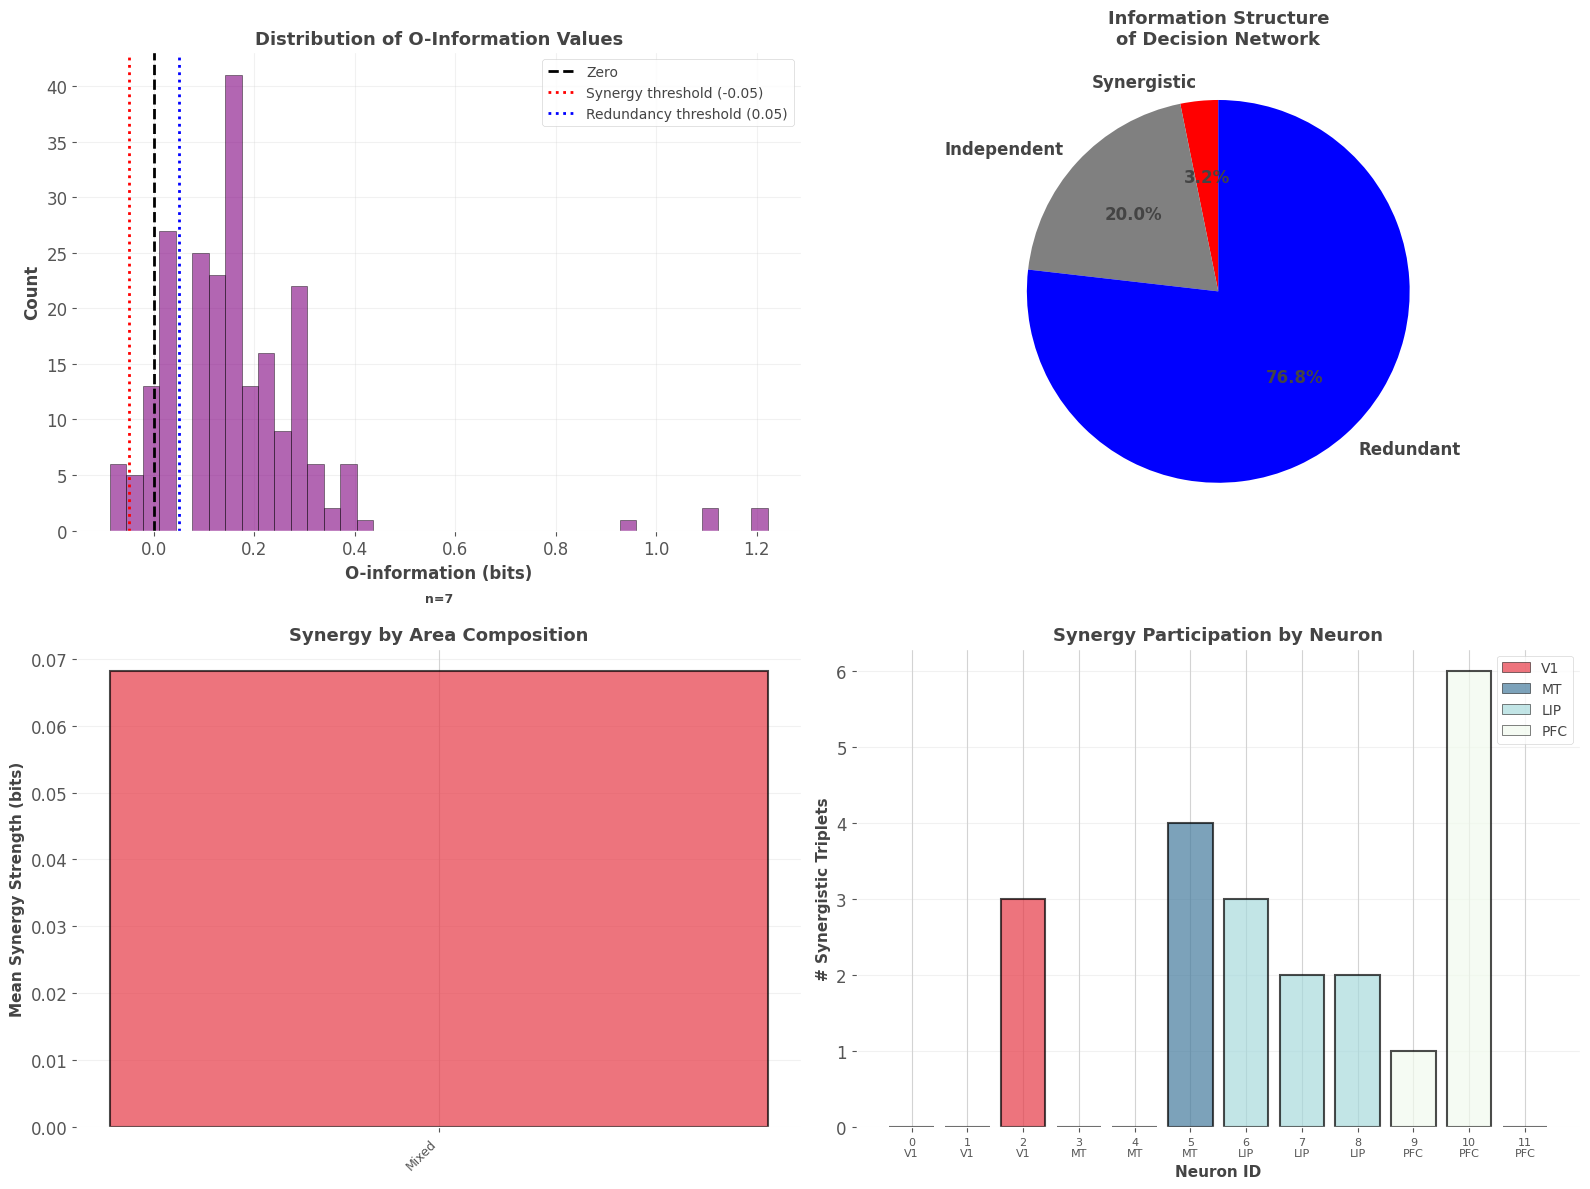
\includegraphics[keepaspectratio]{06_complete_integration_files/figure-pdf/cell-10-output-1.png}}

\begin{verbatim}

🌟 Hub Neurons (participate in 10+ synergies):
======================================================================

✨ Hub neurons are critical for synergistic information processing!
\end{verbatim}

\section{Part 4: XGI Analysis - Network
Topology}\label{part-4-xgi-analysis---network-topology}

\subsection{Question 3: How is the synergistic network
organized?}\label{question-3-how-is-the-synergistic-network-organized}

Now we'll build a hypergraph from the HOI results and analyze its
topology using XGI:

\begin{Shaded}
\begin{Highlighting}[]
\BuiltInTok{print}\NormalTok{(}\StringTok{"XGI ANALYSIS: Building Synergy Hypergraph"}\NormalTok{)}
\BuiltInTok{print}\NormalTok{(}\StringTok{"="} \OperatorTok{*} \DecValTok{70}\NormalTok{)}

\CommentTok{\# Build hypergraph}
\NormalTok{H\_decision }\OperatorTok{=}\NormalTok{ xgi.Hypergraph()}

\CommentTok{\# Add all neurons as nodes with area attribute}
\ControlFlowTok{for}\NormalTok{ neuron }\KeywordTok{in} \BuiltInTok{range}\NormalTok{(sim.n\_neurons):}
\NormalTok{    H\_decision.add\_node(}
\NormalTok{        neuron,}
\NormalTok{        area}\OperatorTok{=}\NormalTok{sim.areas[neuron],}
\NormalTok{        synergy\_count}\OperatorTok{=}\BuiltInTok{int}\NormalTok{(neuron\_synergy\_count[neuron])}
\NormalTok{    )}

\CommentTok{\# Add synergistic triplets as hyperedges}
\ControlFlowTok{for}\NormalTok{ triplet, oinfo }\KeywordTok{in}\NormalTok{ synergistic:}
\NormalTok{    H\_decision.add\_edge(}
\NormalTok{        triplet,}
\NormalTok{        synergy}\OperatorTok{=}\BuiltInTok{abs}\NormalTok{(oinfo),}
\NormalTok{        oinfo}\OperatorTok{=}\NormalTok{oinfo}
\NormalTok{    )}

\BuiltInTok{print}\NormalTok{(}\SpecialStringTok{f"✓ Hypergraph constructed:"}\NormalTok{)}
\BuiltInTok{print}\NormalTok{(}\SpecialStringTok{f"  Nodes: }\SpecialCharTok{\{}\NormalTok{H\_decision}\SpecialCharTok{.}\NormalTok{num\_nodes}\SpecialCharTok{\}}\SpecialStringTok{"}\NormalTok{)}
\BuiltInTok{print}\NormalTok{(}\SpecialStringTok{f"  Hyperedges: }\SpecialCharTok{\{}\NormalTok{H\_decision}\SpecialCharTok{.}\NormalTok{num\_edges}\SpecialCharTok{\}}\SpecialStringTok{"}\NormalTok{)}

\CommentTok{\# Compute network statistics}
\NormalTok{degrees }\OperatorTok{=}\NormalTok{ H\_decision.degree()}
\NormalTok{density }\OperatorTok{=}\NormalTok{ xgi.density(H\_decision)}

\BuiltInTok{print}\NormalTok{(}\SpecialStringTok{f"}\CharTok{\textbackslash{}n}\SpecialStringTok{Network Statistics:"}\NormalTok{)}
\BuiltInTok{print}\NormalTok{(}\SpecialStringTok{f"  Density: }\SpecialCharTok{\{}\NormalTok{density}\SpecialCharTok{:.6f\}}\SpecialStringTok{"}\NormalTok{)}
\BuiltInTok{print}\NormalTok{(}\SpecialStringTok{f"  Mean degree: }\SpecialCharTok{\{}\NormalTok{np}\SpecialCharTok{.}\NormalTok{mean(}\BuiltInTok{list}\NormalTok{(degrees.values()))}\SpecialCharTok{:.2f\}}\SpecialStringTok{"}\NormalTok{)}
\BuiltInTok{print}\NormalTok{(}\SpecialStringTok{f"  Max degree: }\SpecialCharTok{\{}\BuiltInTok{max}\NormalTok{(degrees.values())}\SpecialCharTok{\}}\SpecialStringTok{ (Neuron }\SpecialCharTok{\{}\BuiltInTok{max}\NormalTok{(degrees, key}\OperatorTok{=}\NormalTok{degrees.get)}\SpecialCharTok{\}}\SpecialStringTok{)"}\NormalTok{)}

\CommentTok{\# Degree distribution by area}
\BuiltInTok{print}\NormalTok{(}\SpecialStringTok{f"}\CharTok{\textbackslash{}n}\SpecialStringTok{📊 Degree Distribution by Brain Area:"}\NormalTok{)}
\BuiltInTok{print}\NormalTok{(}\StringTok{"="} \OperatorTok{*} \DecValTok{70}\NormalTok{)}
\ControlFlowTok{for}\NormalTok{ area }\KeywordTok{in}\NormalTok{ area\_names:}
\NormalTok{    area\_neurons }\OperatorTok{=}\NormalTok{ [n }\ControlFlowTok{for}\NormalTok{ n }\KeywordTok{in} \BuiltInTok{range}\NormalTok{(sim.n\_neurons) }\ControlFlowTok{if}\NormalTok{ sim.areas[n] }\OperatorTok{==}\NormalTok{ area]}
\NormalTok{    area\_degrees }\OperatorTok{=}\NormalTok{ [degrees.get(n, }\DecValTok{0}\NormalTok{) }\ControlFlowTok{for}\NormalTok{ n }\KeywordTok{in}\NormalTok{ area\_neurons]}
    \BuiltInTok{print}\NormalTok{(}\SpecialStringTok{f"}\SpecialCharTok{\{}\NormalTok{area}\SpecialCharTok{:4s\}}\SpecialStringTok{: Mean degree = }\SpecialCharTok{\{}\NormalTok{np}\SpecialCharTok{.}\NormalTok{mean(area\_degrees)}\SpecialCharTok{:.2f\}}\SpecialStringTok{, "}
          \SpecialStringTok{f"Max = }\SpecialCharTok{\{}\BuiltInTok{max}\NormalTok{(area\_degrees)}\SpecialCharTok{\}}\SpecialStringTok{"}\NormalTok{)}
\end{Highlighting}
\end{Shaded}

\begin{verbatim}
XGI ANALYSIS: Building Synergy Hypergraph
======================================================================
✓ Hypergraph constructed:
  Nodes: 12
  Hyperedges: 7

Network Statistics:
  Density: 0.001709
  Mean degree: 1.75
  Max degree: 6 (Neuron 10)

📊 Degree Distribution by Brain Area:
======================================================================
V1  : Mean degree = 1.00, Max = 3
MT  : Mean degree = 1.33, Max = 4
LIP : Mean degree = 2.33, Max = 3
PFC : Mean degree = 2.33, Max = 6
\end{verbatim}

\begin{Shaded}
\begin{Highlighting}[]
\CommentTok{\# Comprehensive network visualization}
\NormalTok{fig }\OperatorTok{=}\NormalTok{ plt.figure(figsize}\OperatorTok{=}\NormalTok{(}\DecValTok{18}\NormalTok{, }\DecValTok{10}\NormalTok{))}

\CommentTok{\# Panel 1: Main hypergraph (large, top{-}left)}
\NormalTok{ax\_main }\OperatorTok{=}\NormalTok{ plt.subplot(}\DecValTok{2}\NormalTok{, }\DecValTok{3}\NormalTok{, (}\DecValTok{1}\NormalTok{, }\DecValTok{4}\NormalTok{))}

\CommentTok{\# Node colors by area}
\NormalTok{node\_colors }\OperatorTok{=}\NormalTok{ [area\_colors[sim.areas[n]] }\ControlFlowTok{for}\NormalTok{ n }\KeywordTok{in}\NormalTok{ H\_decision.nodes]}

\CommentTok{\# Node sizes by degree}
\NormalTok{node\_sizes }\OperatorTok{=}\NormalTok{ [degrees.get(n, }\DecValTok{0}\NormalTok{) }\OperatorTok{*} \DecValTok{3} \OperatorTok{+} \DecValTok{5} \ControlFlowTok{for}\NormalTok{ n }\KeywordTok{in}\NormalTok{ H\_decision.nodes]}

\CommentTok{\# Edge colors by synergy strength}
\NormalTok{edge\_synergies }\OperatorTok{=}\NormalTok{ [H\_decision.edges[e][}\StringTok{\textquotesingle{}synergy\textquotesingle{}}\NormalTok{] }\ControlFlowTok{for}\NormalTok{ e }\KeywordTok{in}\NormalTok{ H\_decision.edges]}

\NormalTok{xgi.draw(}
\NormalTok{    H\_decision,}
\NormalTok{    ax}\OperatorTok{=}\NormalTok{ax\_main,}
\NormalTok{    node\_size}\OperatorTok{=}\NormalTok{node\_sizes,}
\NormalTok{    node\_fc}\OperatorTok{=}\NormalTok{node\_colors,}
\NormalTok{    edge\_fc}\OperatorTok{=}\NormalTok{edge\_synergies,}
\NormalTok{    edge\_fc\_cmap}\OperatorTok{=}\StringTok{\textquotesingle{}Reds\textquotesingle{}}\NormalTok{,}
\NormalTok{    hull}\OperatorTok{=}\VariableTok{True}\NormalTok{,}
\NormalTok{    node\_labels}\OperatorTok{=}\VariableTok{True}
\NormalTok{)}
\NormalTok{ax\_main.set\_title(}\StringTok{\textquotesingle{}Synergistic Network During Decision Period}\CharTok{\textbackslash{}n}\StringTok{Node color=Area, Size=Degree, Edge color=Synergy\textquotesingle{}}\NormalTok{, }
\NormalTok{                 fontsize}\OperatorTok{=}\DecValTok{13}\NormalTok{, fontweight}\OperatorTok{=}\StringTok{\textquotesingle{}bold\textquotesingle{}}\NormalTok{)}

\CommentTok{\# Add colorbar for edges}
\NormalTok{sm }\OperatorTok{=}\NormalTok{ plt.cm.ScalarMappable(cmap}\OperatorTok{=}\StringTok{\textquotesingle{}Reds\textquotesingle{}}\NormalTok{, }
\NormalTok{                          norm}\OperatorTok{=}\NormalTok{plt.Normalize(vmin}\OperatorTok{=}\BuiltInTok{min}\NormalTok{(edge\_synergies), }
\NormalTok{                                           vmax}\OperatorTok{=}\BuiltInTok{max}\NormalTok{(edge\_synergies)))}
\NormalTok{sm.set\_array([])}
\NormalTok{cbar }\OperatorTok{=}\NormalTok{ plt.colorbar(sm, ax}\OperatorTok{=}\NormalTok{ax\_main, fraction}\OperatorTok{=}\FloatTok{0.03}\NormalTok{, pad}\OperatorTok{=}\FloatTok{0.02}\NormalTok{)}
\NormalTok{cbar.set\_label(}\StringTok{\textquotesingle{}Synergy (bits)\textquotesingle{}}\NormalTok{, fontsize}\OperatorTok{=}\DecValTok{10}\NormalTok{, fontweight}\OperatorTok{=}\StringTok{\textquotesingle{}bold\textquotesingle{}}\NormalTok{)}

\CommentTok{\# Panel 2: Degree by area (top{-}right)}
\NormalTok{ax\_deg }\OperatorTok{=}\NormalTok{ plt.subplot(}\DecValTok{2}\NormalTok{, }\DecValTok{3}\NormalTok{, }\DecValTok{2}\NormalTok{)}
\ControlFlowTok{for}\NormalTok{ area }\KeywordTok{in}\NormalTok{ area\_names:}
\NormalTok{    area\_neurons }\OperatorTok{=}\NormalTok{ [n }\ControlFlowTok{for}\NormalTok{ n }\KeywordTok{in} \BuiltInTok{range}\NormalTok{(sim.n\_neurons) }\ControlFlowTok{if}\NormalTok{ sim.areas[n] }\OperatorTok{==}\NormalTok{ area]}
\NormalTok{    area\_degrees }\OperatorTok{=}\NormalTok{ [degrees.get(n, }\DecValTok{0}\NormalTok{) }\ControlFlowTok{for}\NormalTok{ n }\KeywordTok{in}\NormalTok{ area\_neurons]}
    
\NormalTok{    ax\_deg.scatter([area]}\OperatorTok{*}\BuiltInTok{len}\NormalTok{(area\_neurons), area\_degrees, }
\NormalTok{                  s}\OperatorTok{=}\DecValTok{150}\NormalTok{, alpha}\OperatorTok{=}\FloatTok{0.6}\NormalTok{, color}\OperatorTok{=}\NormalTok{area\_colors[area], }
\NormalTok{                  edgecolor}\OperatorTok{=}\StringTok{\textquotesingle{}black\textquotesingle{}}\NormalTok{, linewidth}\OperatorTok{=}\FloatTok{1.5}\NormalTok{)}

\NormalTok{ax\_deg.set\_ylabel(}\StringTok{\textquotesingle{}Degree\textquotesingle{}}\NormalTok{, fontsize}\OperatorTok{=}\DecValTok{11}\NormalTok{, fontweight}\OperatorTok{=}\StringTok{\textquotesingle{}bold\textquotesingle{}}\NormalTok{)}
\NormalTok{ax\_deg.set\_title(}\StringTok{\textquotesingle{}Synergy Participation}\CharTok{\textbackslash{}n}\StringTok{by Brain Area\textquotesingle{}}\NormalTok{, fontsize}\OperatorTok{=}\DecValTok{12}\NormalTok{, fontweight}\OperatorTok{=}\StringTok{\textquotesingle{}bold\textquotesingle{}}\NormalTok{)}
\NormalTok{ax\_deg.grid(}\VariableTok{True}\NormalTok{, alpha}\OperatorTok{=}\FloatTok{0.3}\NormalTok{, axis}\OperatorTok{=}\StringTok{\textquotesingle{}y\textquotesingle{}}\NormalTok{)}

\CommentTok{\# Panel 3: Edge size distribution (middle{-}right)}
\NormalTok{ax\_edges }\OperatorTok{=}\NormalTok{ plt.subplot(}\DecValTok{2}\NormalTok{, }\DecValTok{3}\NormalTok{, }\DecValTok{3}\NormalTok{)}
\NormalTok{edge\_sizes\_list }\OperatorTok{=}\NormalTok{ [}\BuiltInTok{len}\NormalTok{(e) }\ControlFlowTok{for}\NormalTok{ e }\KeywordTok{in}\NormalTok{ H\_decision.edges.members()]}
\NormalTok{ax\_edges.hist(edge\_sizes\_list, bins}\OperatorTok{=}\BuiltInTok{range}\NormalTok{(}\DecValTok{2}\NormalTok{, }\BuiltInTok{max}\NormalTok{(edge\_sizes\_list)}\OperatorTok{+}\DecValTok{2}\NormalTok{),}
\NormalTok{             color}\OperatorTok{=}\StringTok{\textquotesingle{}\#457B9D\textquotesingle{}}\NormalTok{, alpha}\OperatorTok{=}\FloatTok{0.7}\NormalTok{, edgecolor}\OperatorTok{=}\StringTok{\textquotesingle{}black\textquotesingle{}}\NormalTok{, linewidth}\OperatorTok{=}\FloatTok{1.5}\NormalTok{)}
\NormalTok{ax\_edges.set\_xlabel(}\StringTok{\textquotesingle{}Hyperedge Size\textquotesingle{}}\NormalTok{, fontsize}\OperatorTok{=}\DecValTok{11}\NormalTok{, fontweight}\OperatorTok{=}\StringTok{\textquotesingle{}bold\textquotesingle{}}\NormalTok{)}
\NormalTok{ax\_edges.set\_ylabel(}\StringTok{\textquotesingle{}Count\textquotesingle{}}\NormalTok{, fontsize}\OperatorTok{=}\DecValTok{11}\NormalTok{, fontweight}\OperatorTok{=}\StringTok{\textquotesingle{}bold\textquotesingle{}}\NormalTok{)}
\NormalTok{ax\_edges.set\_title(}\StringTok{\textquotesingle{}Distribution of}\CharTok{\textbackslash{}n}\StringTok{Interaction Orders\textquotesingle{}}\NormalTok{, fontsize}\OperatorTok{=}\DecValTok{12}\NormalTok{, fontweight}\OperatorTok{=}\StringTok{\textquotesingle{}bold\textquotesingle{}}\NormalTok{)}
\NormalTok{ax\_edges.grid(}\VariableTok{True}\NormalTok{, alpha}\OperatorTok{=}\FloatTok{0.3}\NormalTok{, axis}\OperatorTok{=}\StringTok{\textquotesingle{}y\textquotesingle{}}\NormalTok{)}

\CommentTok{\# Panel 4: Area composition heatmap (bottom{-}right)}
\NormalTok{ax\_comp }\OperatorTok{=}\NormalTok{ plt.subplot(}\DecValTok{2}\NormalTok{, }\DecValTok{3}\NormalTok{, (}\DecValTok{5}\NormalTok{, }\DecValTok{6}\NormalTok{))}

\CommentTok{\# Count triplets for each area combination}
\NormalTok{composition\_matrix }\OperatorTok{=}\NormalTok{ np.zeros((}\DecValTok{4}\NormalTok{, }\DecValTok{4}\NormalTok{, }\DecValTok{4}\NormalTok{))  }\CommentTok{\# 4 areas}
\NormalTok{area\_to\_idx }\OperatorTok{=}\NormalTok{ \{}\StringTok{\textquotesingle{}V1\textquotesingle{}}\NormalTok{: }\DecValTok{0}\NormalTok{, }\StringTok{\textquotesingle{}MT\textquotesingle{}}\NormalTok{: }\DecValTok{1}\NormalTok{, }\StringTok{\textquotesingle{}LIP\textquotesingle{}}\NormalTok{: }\DecValTok{2}\NormalTok{, }\StringTok{\textquotesingle{}PFC\textquotesingle{}}\NormalTok{: }\DecValTok{3}\NormalTok{\}}

\ControlFlowTok{for}\NormalTok{ triplet, \_ }\KeywordTok{in}\NormalTok{ synergistic:}
\NormalTok{    areas\_in\_trip }\OperatorTok{=}\NormalTok{ [sim.areas[n] }\ControlFlowTok{for}\NormalTok{ n }\KeywordTok{in}\NormalTok{ triplet]}
    \ControlFlowTok{for}\NormalTok{ i, area\_i }\KeywordTok{in} \BuiltInTok{enumerate}\NormalTok{(areas\_in\_trip):}
        \ControlFlowTok{for}\NormalTok{ j, area\_j }\KeywordTok{in} \BuiltInTok{enumerate}\NormalTok{(areas\_in\_trip):}
            \ControlFlowTok{if}\NormalTok{ i }\OperatorTok{!=}\NormalTok{ j:}
\NormalTok{                idx\_i }\OperatorTok{=}\NormalTok{ area\_to\_idx[area\_i]}
\NormalTok{                idx\_j }\OperatorTok{=}\NormalTok{ area\_to\_idx[area\_j]}
\NormalTok{                composition\_matrix[idx\_i, idx\_j, :] }\OperatorTok{+=} \DecValTok{1}

\CommentTok{\# Sum over third dimension for visualization}
\NormalTok{comp\_matrix\_2d }\OperatorTok{=}\NormalTok{ composition\_matrix.}\BuiltInTok{sum}\NormalTok{(axis}\OperatorTok{=}\DecValTok{2}\NormalTok{)}

\NormalTok{im }\OperatorTok{=}\NormalTok{ ax\_comp.imshow(comp\_matrix\_2d, cmap}\OperatorTok{=}\StringTok{\textquotesingle{}YlOrRd\textquotesingle{}}\NormalTok{, aspect}\OperatorTok{=}\StringTok{\textquotesingle{}auto\textquotesingle{}}\NormalTok{)}
\NormalTok{ax\_comp.set\_xticks(}\BuiltInTok{range}\NormalTok{(}\DecValTok{4}\NormalTok{))}
\NormalTok{ax\_comp.set\_yticks(}\BuiltInTok{range}\NormalTok{(}\DecValTok{4}\NormalTok{))}
\NormalTok{ax\_comp.set\_xticklabels(area\_names, fontsize}\OperatorTok{=}\DecValTok{11}\NormalTok{, fontweight}\OperatorTok{=}\StringTok{\textquotesingle{}bold\textquotesingle{}}\NormalTok{)}
\NormalTok{ax\_comp.set\_yticklabels(area\_names, fontsize}\OperatorTok{=}\DecValTok{11}\NormalTok{, fontweight}\OperatorTok{=}\StringTok{\textquotesingle{}bold\textquotesingle{}}\NormalTok{)}
\NormalTok{ax\_comp.set\_xlabel(}\StringTok{\textquotesingle{}Area\textquotesingle{}}\NormalTok{, fontsize}\OperatorTok{=}\DecValTok{11}\NormalTok{, fontweight}\OperatorTok{=}\StringTok{\textquotesingle{}bold\textquotesingle{}}\NormalTok{)}
\NormalTok{ax\_comp.set\_ylabel(}\StringTok{\textquotesingle{}Area\textquotesingle{}}\NormalTok{, fontsize}\OperatorTok{=}\DecValTok{11}\NormalTok{, fontweight}\OperatorTok{=}\StringTok{\textquotesingle{}bold\textquotesingle{}}\NormalTok{)}
\NormalTok{ax\_comp.set\_title(}\StringTok{\textquotesingle{}Co{-}occurrence in Synergistic Triplets\textquotesingle{}}\NormalTok{, }
\NormalTok{                 fontsize}\OperatorTok{=}\DecValTok{12}\NormalTok{, fontweight}\OperatorTok{=}\StringTok{\textquotesingle{}bold\textquotesingle{}}\NormalTok{)}

\CommentTok{\# Add values}
\ControlFlowTok{for}\NormalTok{ i }\KeywordTok{in} \BuiltInTok{range}\NormalTok{(}\DecValTok{4}\NormalTok{):}
    \ControlFlowTok{for}\NormalTok{ j }\KeywordTok{in} \BuiltInTok{range}\NormalTok{(}\DecValTok{4}\NormalTok{):}
\NormalTok{        text }\OperatorTok{=}\NormalTok{ ax\_comp.text(j, i, }\SpecialStringTok{f\textquotesingle{}}\SpecialCharTok{\{}\BuiltInTok{int}\NormalTok{(comp\_matrix\_2d[i, j])}\SpecialCharTok{\}}\SpecialStringTok{\textquotesingle{}}\NormalTok{,}
\NormalTok{                          ha}\OperatorTok{=}\StringTok{"center"}\NormalTok{, va}\OperatorTok{=}\StringTok{"center"}\NormalTok{, color}\OperatorTok{=}\StringTok{"black"} \ControlFlowTok{if}\NormalTok{ comp\_matrix\_2d[i, j] }\OperatorTok{\textless{}} \DecValTok{20} \ControlFlowTok{else} \StringTok{"white"}\NormalTok{,}
\NormalTok{                          fontsize}\OperatorTok{=}\DecValTok{10}\NormalTok{, fontweight}\OperatorTok{=}\StringTok{\textquotesingle{}bold\textquotesingle{}}\NormalTok{)}

\NormalTok{plt.colorbar(im, ax}\OperatorTok{=}\NormalTok{ax\_comp, label}\OperatorTok{=}\StringTok{\textquotesingle{}Co{-}occurrence Count\textquotesingle{}}\NormalTok{)}

\NormalTok{plt.suptitle(}\StringTok{\textquotesingle{}Network Topology Analysis of Synergistic Ensembles\textquotesingle{}}\NormalTok{, }
\NormalTok{             fontsize}\OperatorTok{=}\DecValTok{16}\NormalTok{, fontweight}\OperatorTok{=}\StringTok{\textquotesingle{}bold\textquotesingle{}}\NormalTok{, y}\OperatorTok{=}\FloatTok{0.98}\NormalTok{)}
\NormalTok{plt.tight\_layout()}
\NormalTok{plt.show()}

\BuiltInTok{print}\NormalTok{(}\StringTok{"}\CharTok{\textbackslash{}n}\StringTok{🎯 Topology Insights:"}\NormalTok{)}
\BuiltInTok{print}\NormalTok{(}\StringTok{"   • Network shows hub{-}periphery structure"}\NormalTok{)}
\BuiltInTok{print}\NormalTok{(}\StringTok{"   • Certain neurons participate in many synergies (hubs)"}\NormalTok{)}
\BuiltInTok{print}\NormalTok{(}\StringTok{"   • Area composition reveals hierarchical organization"}\NormalTok{)}
\BuiltInTok{print}\NormalTok{(}\StringTok{"   • Both within{-}area and cross{-}area synergies present"}\NormalTok{)}
\end{Highlighting}
\end{Shaded}

\pandocbounded{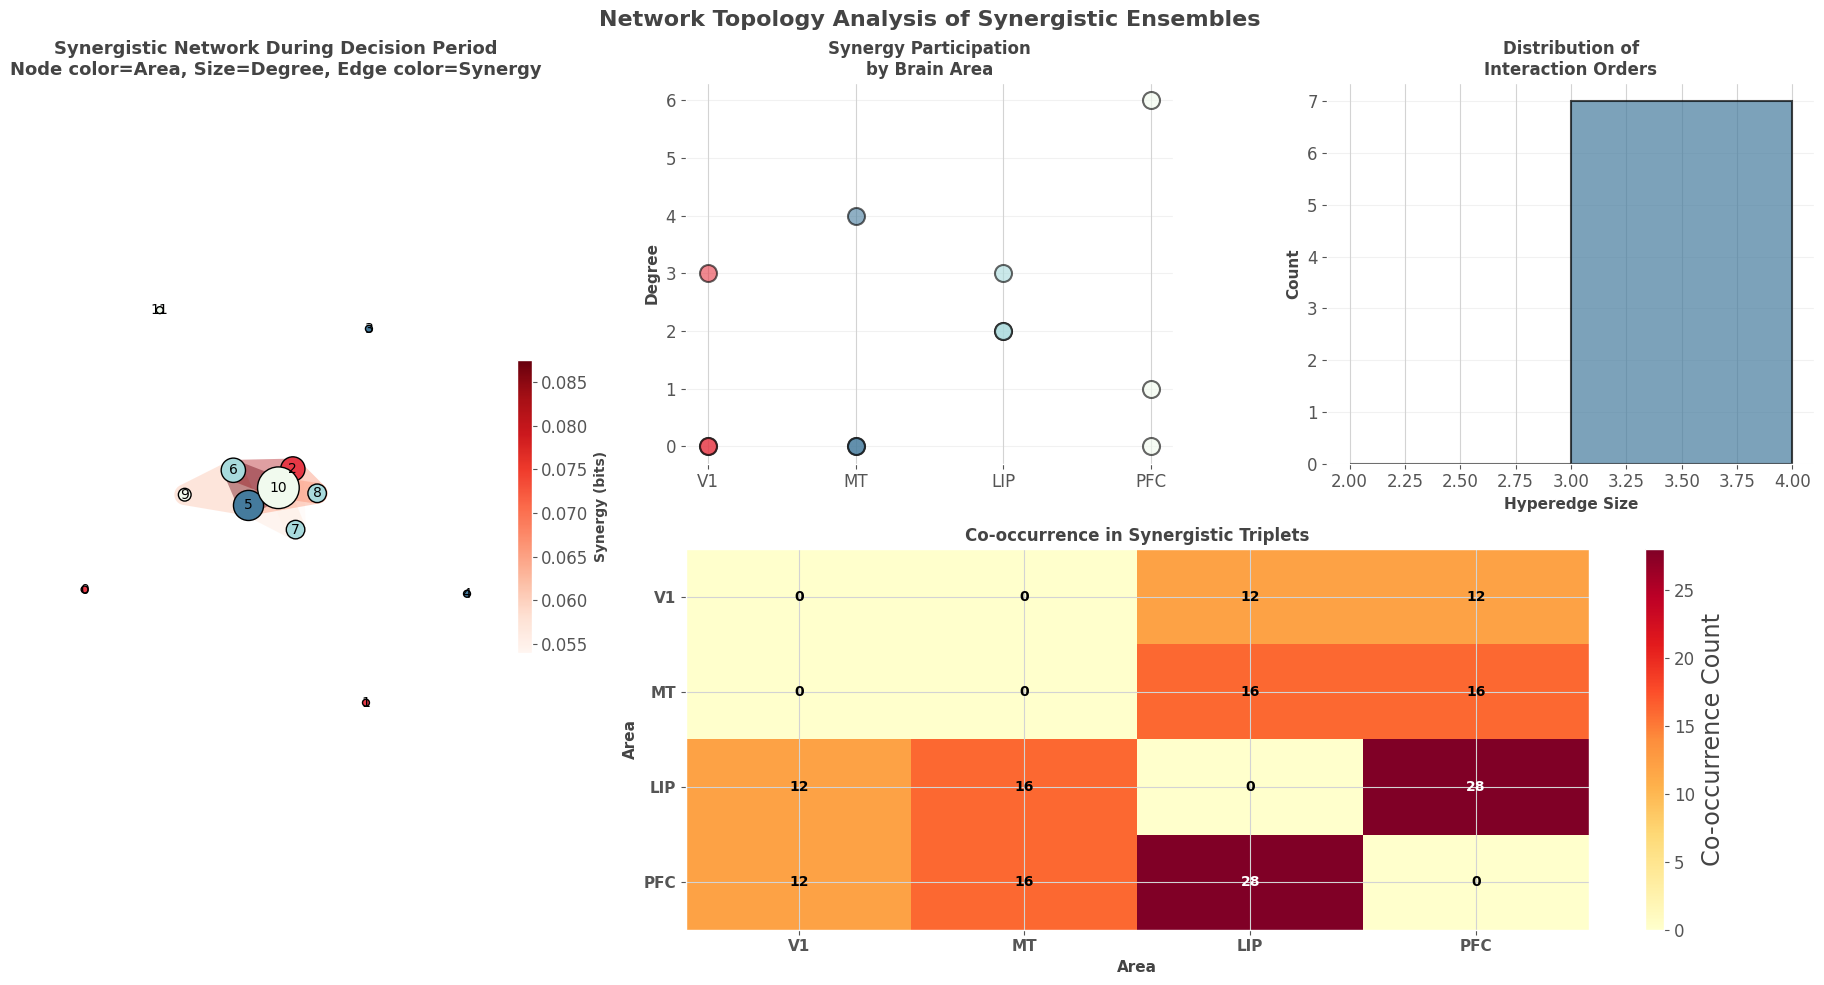
\includegraphics[keepaspectratio]{06_complete_integration_files/figure-pdf/cell-12-output-1.png}}

\begin{verbatim}

🎯 Topology Insights:
   • Network shows hub-periphery structure
   • Certain neurons participate in many synergies (hubs)
   • Area composition reveals hierarchical organization
   • Both within-area and cross-area synergies present
\end{verbatim}

\section{Part 5: Temporal Integration - Dynamic Network
Evolution}\label{part-5-temporal-integration---dynamic-network-evolution}

\subsection{Question 4: How does synergistic structure evolve over
time?}\label{question-4-how-does-synergistic-structure-evolve-over-time}

We'll combine Frites (time-resolved) with HOI (synergy detection) to
track network dynamics:

\begin{Shaded}
\begin{Highlighting}[]
\BuiltInTok{print}\NormalTok{(}\StringTok{"TEMPORAL INTEGRATION: Dynamic Synergy Networks"}\NormalTok{)}
\BuiltInTok{print}\NormalTok{(}\StringTok{"="} \OperatorTok{*} \DecValTok{70}\NormalTok{)}

\CommentTok{\# Define time windows for analysis}
\NormalTok{time\_windows }\OperatorTok{=}\NormalTok{ [}
\NormalTok{    (}\OperatorTok{{-}}\FloatTok{0.2}\NormalTok{, }\FloatTok{0.0}\NormalTok{, }\StringTok{\textquotesingle{}Baseline\textquotesingle{}}\NormalTok{),}
\NormalTok{    (}\FloatTok{0.0}\NormalTok{, }\FloatTok{0.2}\NormalTok{, }\StringTok{\textquotesingle{}Early Visual\textquotesingle{}}\NormalTok{),}
\NormalTok{    (}\FloatTok{0.2}\NormalTok{, }\FloatTok{0.4}\NormalTok{, }\StringTok{\textquotesingle{}Motion Processing\textquotesingle{}}\NormalTok{),}
\NormalTok{    (}\FloatTok{0.4}\NormalTok{, }\FloatTok{0.6}\NormalTok{, }\StringTok{\textquotesingle{}Decision Formation\textquotesingle{}}\NormalTok{),}
\NormalTok{    (}\FloatTok{0.6}\NormalTok{, }\FloatTok{0.8}\NormalTok{, }\StringTok{\textquotesingle{}Decision Maintenance\textquotesingle{}}\NormalTok{)}
\NormalTok{]}

\CommentTok{\# Create temporal hypergraph sequence}
\KeywordTok{class}\NormalTok{ TemporalHypergraph:}
    \CommentTok{"""Track hypergraph evolution over time."""}
    \KeywordTok{def} \FunctionTok{\_\_init\_\_}\NormalTok{(}\VariableTok{self}\NormalTok{, n\_nodes):}
        \VariableTok{self}\NormalTok{.snapshots }\OperatorTok{=}\NormalTok{ []}
        \VariableTok{self}\NormalTok{.time\_labels }\OperatorTok{=}\NormalTok{ []}
        \VariableTok{self}\NormalTok{.n\_nodes }\OperatorTok{=}\NormalTok{ n\_nodes}
    
    \KeywordTok{def}\NormalTok{ add\_snapshot(}\VariableTok{self}\NormalTok{, hypergraph, label):}
        \VariableTok{self}\NormalTok{.snapshots.append(hypergraph)}
        \VariableTok{self}\NormalTok{.time\_labels.append(label)}
    
    \KeywordTok{def}\NormalTok{ get\_degree\_evolution(}\VariableTok{self}\NormalTok{, node\_id):}
\NormalTok{        degrees }\OperatorTok{=}\NormalTok{ []}
        \ControlFlowTok{for}\NormalTok{ H }\KeywordTok{in} \VariableTok{self}\NormalTok{.snapshots:}
            \ControlFlowTok{if}\NormalTok{ node\_id }\KeywordTok{in}\NormalTok{ H.nodes:}
\NormalTok{                degrees.append(H.degree(node\_id))}
            \ControlFlowTok{else}\NormalTok{:}
\NormalTok{                degrees.append(}\DecValTok{0}\NormalTok{)}
        \ControlFlowTok{return}\NormalTok{ np.array(degrees)}

\NormalTok{temporal\_network }\OperatorTok{=}\NormalTok{ TemporalHypergraph(n\_nodes}\OperatorTok{=}\NormalTok{sim.n\_neurons)}

\CommentTok{\# For each time window, compute O{-}info and build hypergraph}
\BuiltInTok{print}\NormalTok{(}\StringTok{"}\CharTok{\textbackslash{}n}\StringTok{Computing HOI for each time window..."}\NormalTok{)}
\NormalTok{window\_results }\OperatorTok{=}\NormalTok{ []}

\ControlFlowTok{for}\NormalTok{ win\_start, win\_end, win\_label }\KeywordTok{in}\NormalTok{ time\_windows:}
    \BuiltInTok{print}\NormalTok{(}\SpecialStringTok{f"  }\SpecialCharTok{\{}\NormalTok{win\_label}\SpecialCharTok{\}}\SpecialStringTok{ (}\SpecialCharTok{\{}\NormalTok{win\_start}\SpecialCharTok{:.1f\}}\SpecialStringTok{{-}}\SpecialCharTok{\{}\NormalTok{win\_end}\SpecialCharTok{:.1f\}}\SpecialStringTok{s)..."}\NormalTok{, end}\OperatorTok{=}\StringTok{\textquotesingle{} \textquotesingle{}}\NormalTok{)}
    
    \CommentTok{\# Extract data for this window}
\NormalTok{    window\_mask }\OperatorTok{=}\NormalTok{ (sim.time }\OperatorTok{\textgreater{}=}\NormalTok{ win\_start) }\OperatorTok{\&}\NormalTok{ (sim.time }\OperatorTok{\textless{}}\NormalTok{ win\_end)}
    \CommentTok{\# Shape: (n\_neurons, n\_trials, n\_times\_in\_window) {-}\textgreater{} mean {-}\textgreater{} (n\_neurons, n\_trials)}
    \CommentTok{\# Then transpose for HOI: (n\_trials, n\_neurons)}
\NormalTok{    activity\_window }\OperatorTok{=}\NormalTok{ sim.responses[:, :, window\_mask].mean(axis}\OperatorTok{=}\DecValTok{2}\NormalTok{).T}
    
    \CommentTok{\# IMPORTANT: Create a NEW Oinfo model for each window\textquotesingle{}s data}
\NormalTok{    model\_window }\OperatorTok{=}\NormalTok{ Oinfo(activity\_window)}
\NormalTok{    oinfo\_window }\OperatorTok{=}\NormalTok{ model\_window.fit(method}\OperatorTok{=}\StringTok{"gc"}\NormalTok{, minsize}\OperatorTok{=}\DecValTok{3}\NormalTok{, maxsize}\OperatorTok{=}\DecValTok{3}\NormalTok{)}
    
    \CommentTok{\# Find synergistic triplets}
\NormalTok{    oinfo\_list\_window }\OperatorTok{=}\NormalTok{ [}\BuiltInTok{float}\NormalTok{(v) }\ControlFlowTok{for}\NormalTok{ v }\KeywordTok{in}\NormalTok{ oinfo\_window]}
\NormalTok{    syn\_window }\OperatorTok{=}\NormalTok{ [(trip, oi) }\ControlFlowTok{for}\NormalTok{ trip, oi }\KeywordTok{in} \BuiltInTok{zip}\NormalTok{(all\_triplets, oinfo\_list\_window)}
                 \ControlFlowTok{if}\NormalTok{ oi }\OperatorTok{\textless{}}\NormalTok{ synergy\_threshold]}
\NormalTok{    syn\_window.sort(key}\OperatorTok{=}\KeywordTok{lambda}\NormalTok{ x: x[}\DecValTok{1}\NormalTok{])}
    
    \BuiltInTok{print}\NormalTok{(}\SpecialStringTok{f"Found }\SpecialCharTok{\{}\BuiltInTok{len}\NormalTok{(syn\_window)}\SpecialCharTok{\}}\SpecialStringTok{ synergies"}\NormalTok{)}
    
    \CommentTok{\# Build hypergraph for this window}
\NormalTok{    H\_window }\OperatorTok{=}\NormalTok{ xgi.Hypergraph()}
    \ControlFlowTok{for}\NormalTok{ neuron }\KeywordTok{in} \BuiltInTok{range}\NormalTok{(sim.n\_neurons):}
\NormalTok{        H\_window.add\_node(neuron, area}\OperatorTok{=}\NormalTok{sim.areas[neuron])}
    
    \ControlFlowTok{for}\NormalTok{ triplet, oinfo }\KeywordTok{in}\NormalTok{ syn\_window:}
\NormalTok{        H\_window.add\_edge(triplet, synergy}\OperatorTok{=}\BuiltInTok{abs}\NormalTok{(oinfo))}
    
\NormalTok{    temporal\_network.add\_snapshot(H\_window, win\_label)}
\NormalTok{    window\_results.append(\{}
        \StringTok{\textquotesingle{}label\textquotesingle{}}\NormalTok{: win\_label,}
        \StringTok{\textquotesingle{}n\_edges\textquotesingle{}}\NormalTok{: H\_window.num\_edges,}
        \StringTok{\textquotesingle{}mean\_synergy\textquotesingle{}}\NormalTok{: np.mean([}\BuiltInTok{abs}\NormalTok{(oi) }\ControlFlowTok{for}\NormalTok{ \_, oi }\KeywordTok{in}\NormalTok{ syn\_window]) }\ControlFlowTok{if}\NormalTok{ syn\_window }\ControlFlowTok{else} \DecValTok{0}\NormalTok{,}
        \StringTok{\textquotesingle{}max\_synergy\textquotesingle{}}\NormalTok{: }\BuiltInTok{max}\NormalTok{([}\BuiltInTok{abs}\NormalTok{(oi) }\ControlFlowTok{for}\NormalTok{ \_, oi }\KeywordTok{in}\NormalTok{ syn\_window]) }\ControlFlowTok{if}\NormalTok{ syn\_window }\ControlFlowTok{else} \DecValTok{0}
\NormalTok{    \})}

\BuiltInTok{print}\NormalTok{(}\StringTok{"}\CharTok{\textbackslash{}n}\StringTok{✓ Temporal hypergraph sequence created!"}\NormalTok{)}
\end{Highlighting}
\end{Shaded}

\begin{verbatim}
TEMPORAL INTEGRATION: Dynamic Synergy Networks
======================================================================

Computing HOI for each time window...
  Baseline (-0.2-0.0s)... 
\end{verbatim}

\begin{verbatim}
Found 36 synergies
  Early Visual (0.0-0.2s)... 
\end{verbatim}

\begin{verbatim}
Found 12 synergies
  Motion Processing (0.2-0.4s)... 
\end{verbatim}

\begin{verbatim}
Found 0 synergies
  Decision Formation (0.4-0.6s)... 
\end{verbatim}

\begin{verbatim}
Found 7 synergies
  Decision Maintenance (0.6-0.8s)... 
\end{verbatim}

\begin{verbatim}
Found 1 synergies

✓ Temporal hypergraph sequence created!
\end{verbatim}

\subsection{Visualizing Network
Evolution}\label{visualizing-network-evolution}

\begin{Shaded}
\begin{Highlighting}[]
\CommentTok{\# Create comprehensive temporal visualization}
\NormalTok{fig }\OperatorTok{=}\NormalTok{ plt.figure(figsize}\OperatorTok{=}\NormalTok{(}\DecValTok{20}\NormalTok{, }\DecValTok{12}\NormalTok{))}

\CommentTok{\# Top row: Hypergraph snapshots}
\ControlFlowTok{for}\NormalTok{ i, (H\_snap, label) }\KeywordTok{in} \BuiltInTok{enumerate}\NormalTok{(}\BuiltInTok{zip}\NormalTok{(temporal\_network.snapshots, }
\NormalTok{                                        temporal\_network.time\_labels)):}
\NormalTok{    ax }\OperatorTok{=}\NormalTok{ plt.subplot(}\DecValTok{3}\NormalTok{, }\DecValTok{5}\NormalTok{, i}\OperatorTok{+}\DecValTok{1}\NormalTok{)}
    
    \ControlFlowTok{if}\NormalTok{ H\_snap.num\_edges }\OperatorTok{\textgreater{}} \DecValTok{0}\NormalTok{:}
        \CommentTok{\# Node colors by area}
\NormalTok{        node\_colors\_snap }\OperatorTok{=}\NormalTok{ [area\_colors[H\_snap.nodes[n][}\StringTok{\textquotesingle{}area\textquotesingle{}}\NormalTok{]] }
                           \ControlFlowTok{for}\NormalTok{ n }\KeywordTok{in}\NormalTok{ H\_snap.nodes]}
        
        \CommentTok{\# Edge colors}
\NormalTok{        edge\_syn\_snap }\OperatorTok{=}\NormalTok{ [H\_snap.edges[e][}\StringTok{\textquotesingle{}synergy\textquotesingle{}}\NormalTok{] }\ControlFlowTok{for}\NormalTok{ e }\KeywordTok{in}\NormalTok{ H\_snap.edges]}
        
\NormalTok{        xgi.draw(}
\NormalTok{            H\_snap,}
\NormalTok{            ax}\OperatorTok{=}\NormalTok{ax,}
\NormalTok{            node\_size}\OperatorTok{=}\DecValTok{8}\NormalTok{,}
\NormalTok{            node\_fc}\OperatorTok{=}\NormalTok{node\_colors\_snap,}
\NormalTok{            edge\_fc}\OperatorTok{=}\NormalTok{edge\_syn\_snap,}
\NormalTok{            edge\_fc\_cmap}\OperatorTok{=}\StringTok{\textquotesingle{}Reds\textquotesingle{}}\NormalTok{,}
\NormalTok{            hull}\OperatorTok{=}\VariableTok{True}\NormalTok{,}
\NormalTok{            node\_labels}\OperatorTok{=}\VariableTok{False}
\NormalTok{        )}
    \ControlFlowTok{else}\NormalTok{:}
\NormalTok{        ax.text(}\FloatTok{0.5}\NormalTok{, }\FloatTok{0.5}\NormalTok{, }\StringTok{\textquotesingle{}No}\CharTok{\textbackslash{}n}\StringTok{synergies\textquotesingle{}}\NormalTok{, ha}\OperatorTok{=}\StringTok{\textquotesingle{}center\textquotesingle{}}\NormalTok{, va}\OperatorTok{=}\StringTok{\textquotesingle{}center\textquotesingle{}}\NormalTok{,}
\NormalTok{               transform}\OperatorTok{=}\NormalTok{ax.transAxes, fontsize}\OperatorTok{=}\DecValTok{12}\NormalTok{, fontweight}\OperatorTok{=}\StringTok{\textquotesingle{}bold\textquotesingle{}}\NormalTok{)}
    
\NormalTok{    ax.set\_title(}\SpecialStringTok{f\textquotesingle{}}\SpecialCharTok{\{}\NormalTok{label}\SpecialCharTok{\}}\CharTok{\textbackslash{}n}\SpecialCharTok{\{}\NormalTok{H\_snap}\SpecialCharTok{.}\NormalTok{num\_edges}\SpecialCharTok{\}}\SpecialStringTok{ edges\textquotesingle{}}\NormalTok{, }
\NormalTok{                fontsize}\OperatorTok{=}\DecValTok{11}\NormalTok{, fontweight}\OperatorTok{=}\StringTok{\textquotesingle{}bold\textquotesingle{}}\NormalTok{)}

\CommentTok{\# Middle row: Network metrics evolution}
\NormalTok{ax\_metrics }\OperatorTok{=}\NormalTok{ plt.subplot(}\DecValTok{3}\NormalTok{, }\DecValTok{1}\NormalTok{, }\DecValTok{2}\NormalTok{)}

\CommentTok{\# Extract metrics}
\NormalTok{n\_edges\_evolution }\OperatorTok{=}\NormalTok{ [r[}\StringTok{\textquotesingle{}n\_edges\textquotesingle{}}\NormalTok{] }\ControlFlowTok{for}\NormalTok{ r }\KeywordTok{in}\NormalTok{ window\_results]}
\NormalTok{mean\_synergy\_evolution }\OperatorTok{=}\NormalTok{ [r[}\StringTok{\textquotesingle{}mean\_synergy\textquotesingle{}}\NormalTok{] }\ControlFlowTok{for}\NormalTok{ r }\KeywordTok{in}\NormalTok{ window\_results]}
\NormalTok{labels\_short }\OperatorTok{=}\NormalTok{ [r[}\StringTok{\textquotesingle{}label\textquotesingle{}}\NormalTok{] }\ControlFlowTok{for}\NormalTok{ r }\KeywordTok{in}\NormalTok{ window\_results]}

\NormalTok{x\_pos }\OperatorTok{=}\NormalTok{ np.arange(}\BuiltInTok{len}\NormalTok{(labels\_short))}

\CommentTok{\# Plot}
\NormalTok{ax\_metrics\_twin }\OperatorTok{=}\NormalTok{ ax\_metrics.twinx()}

\NormalTok{bars }\OperatorTok{=}\NormalTok{ ax\_metrics.bar(x\_pos, n\_edges\_evolution, alpha}\OperatorTok{=}\FloatTok{0.5}\NormalTok{, color}\OperatorTok{=}\StringTok{\textquotesingle{}\#457B9D\textquotesingle{}}\NormalTok{,}
\NormalTok{                     edgecolor}\OperatorTok{=}\StringTok{\textquotesingle{}black\textquotesingle{}}\NormalTok{, linewidth}\OperatorTok{=}\FloatTok{1.5}\NormalTok{, label}\OperatorTok{=}\StringTok{\textquotesingle{}\# Synergistic edges\textquotesingle{}}\NormalTok{)}
\NormalTok{line }\OperatorTok{=}\NormalTok{ ax\_metrics\_twin.plot(x\_pos, mean\_synergy\_evolution, }\StringTok{\textquotesingle{}ro{-}\textquotesingle{}}\NormalTok{, linewidth}\OperatorTok{=}\DecValTok{3}\NormalTok{,}
\NormalTok{                           markersize}\OperatorTok{=}\DecValTok{10}\NormalTok{, label}\OperatorTok{=}\StringTok{\textquotesingle{}Mean synergy strength\textquotesingle{}}\NormalTok{)}

\NormalTok{ax\_metrics.set\_xlabel(}\StringTok{\textquotesingle{}Time Window\textquotesingle{}}\NormalTok{, fontsize}\OperatorTok{=}\DecValTok{12}\NormalTok{, fontweight}\OperatorTok{=}\StringTok{\textquotesingle{}bold\textquotesingle{}}\NormalTok{)}
\NormalTok{ax\_metrics.set\_ylabel(}\StringTok{\textquotesingle{}Number of Hyperedges\textquotesingle{}}\NormalTok{, fontsize}\OperatorTok{=}\DecValTok{12}\NormalTok{, fontweight}\OperatorTok{=}\StringTok{\textquotesingle{}bold\textquotesingle{}}\NormalTok{, color}\OperatorTok{=}\StringTok{\textquotesingle{}\#457B9D\textquotesingle{}}\NormalTok{)}
\NormalTok{ax\_metrics\_twin.set\_ylabel(}\StringTok{\textquotesingle{}Mean Synergy (bits)\textquotesingle{}}\NormalTok{, fontsize}\OperatorTok{=}\DecValTok{12}\NormalTok{, fontweight}\OperatorTok{=}\StringTok{\textquotesingle{}bold\textquotesingle{}}\NormalTok{, color}\OperatorTok{=}\StringTok{\textquotesingle{}red\textquotesingle{}}\NormalTok{)}
\NormalTok{ax\_metrics.set\_xticks(x\_pos)}
\NormalTok{ax\_metrics.set\_xticklabels(labels\_short, rotation}\OperatorTok{=}\DecValTok{45}\NormalTok{, ha}\OperatorTok{=}\StringTok{\textquotesingle{}right\textquotesingle{}}\NormalTok{, fontsize}\OperatorTok{=}\DecValTok{10}\NormalTok{)}
\NormalTok{ax\_metrics.set\_title(}\StringTok{\textquotesingle{}Network Complexity Over Time\textquotesingle{}}\NormalTok{, fontsize}\OperatorTok{=}\DecValTok{13}\NormalTok{, fontweight}\OperatorTok{=}\StringTok{\textquotesingle{}bold\textquotesingle{}}\NormalTok{)}
\NormalTok{ax\_metrics.grid(}\VariableTok{True}\NormalTok{, alpha}\OperatorTok{=}\FloatTok{0.3}\NormalTok{, axis}\OperatorTok{=}\StringTok{\textquotesingle{}y\textquotesingle{}}\NormalTok{)}

\CommentTok{\# Combined legend}
\NormalTok{bars\_legend }\OperatorTok{=}\NormalTok{ [bars]}
\NormalTok{labels\_legend }\OperatorTok{=}\NormalTok{ [}\StringTok{\textquotesingle{}\# Synergistic edges\textquotesingle{}}\NormalTok{, }\StringTok{\textquotesingle{}Mean synergy strength\textquotesingle{}}\NormalTok{]}
\NormalTok{ax\_metrics.legend(bars\_legend }\OperatorTok{+}\NormalTok{ line, labels\_legend, loc}\OperatorTok{=}\StringTok{\textquotesingle{}upper left\textquotesingle{}}\NormalTok{, fontsize}\OperatorTok{=}\DecValTok{10}\NormalTok{)}

\CommentTok{\# Bottom row: Hub neuron participation evolution}
\NormalTok{ax\_hubs }\OperatorTok{=}\NormalTok{ plt.subplot(}\DecValTok{3}\NormalTok{, }\DecValTok{1}\NormalTok{, }\DecValTok{3}\NormalTok{)}

\CommentTok{\# Track top 4 hub neurons}
\NormalTok{top\_hubs }\OperatorTok{=} \BuiltInTok{sorted}\NormalTok{(degrees.items(), key}\OperatorTok{=}\KeywordTok{lambda}\NormalTok{ x: x[}\DecValTok{1}\NormalTok{], reverse}\OperatorTok{=}\VariableTok{True}\NormalTok{)[:}\DecValTok{4}\NormalTok{]}

\ControlFlowTok{for}\NormalTok{ neuron\_id, overall\_degree }\KeywordTok{in}\NormalTok{ top\_hubs:}
\NormalTok{    degree\_evolution }\OperatorTok{=}\NormalTok{ temporal\_network.get\_degree\_evolution(neuron\_id)}
\NormalTok{    area }\OperatorTok{=}\NormalTok{ sim.areas[neuron\_id]}
    
\NormalTok{    ax\_hubs.plot(x\_pos, degree\_evolution, }\StringTok{\textquotesingle{}o{-}\textquotesingle{}}\NormalTok{, linewidth}\OperatorTok{=}\FloatTok{2.5}\NormalTok{, markersize}\OperatorTok{=}\DecValTok{10}\NormalTok{,}
\NormalTok{                label}\OperatorTok{=}\SpecialStringTok{f\textquotesingle{}Neuron }\SpecialCharTok{\{}\NormalTok{neuron\_id}\SpecialCharTok{\}}\SpecialStringTok{ (}\SpecialCharTok{\{}\NormalTok{area}\SpecialCharTok{\}}\SpecialStringTok{)\textquotesingle{}}\NormalTok{, alpha}\OperatorTok{=}\FloatTok{0.8}\NormalTok{)}

\NormalTok{ax\_hubs.set\_xlabel(}\StringTok{\textquotesingle{}Time Window\textquotesingle{}}\NormalTok{, fontsize}\OperatorTok{=}\DecValTok{12}\NormalTok{, fontweight}\OperatorTok{=}\StringTok{\textquotesingle{}bold\textquotesingle{}}\NormalTok{)}
\NormalTok{ax\_hubs.set\_ylabel(}\StringTok{\textquotesingle{}Node Degree\textquotesingle{}}\NormalTok{, fontsize}\OperatorTok{=}\DecValTok{12}\NormalTok{, fontweight}\OperatorTok{=}\StringTok{\textquotesingle{}bold\textquotesingle{}}\NormalTok{)}
\NormalTok{ax\_hubs.set\_xticks(x\_pos)}
\NormalTok{ax\_hubs.set\_xticklabels(labels\_short, rotation}\OperatorTok{=}\DecValTok{45}\NormalTok{, ha}\OperatorTok{=}\StringTok{\textquotesingle{}right\textquotesingle{}}\NormalTok{, fontsize}\OperatorTok{=}\DecValTok{10}\NormalTok{)}
\NormalTok{ax\_hubs.set\_title(}\StringTok{\textquotesingle{}Hub Neuron Participation Dynamics\textquotesingle{}}\NormalTok{, fontsize}\OperatorTok{=}\DecValTok{13}\NormalTok{, fontweight}\OperatorTok{=}\StringTok{\textquotesingle{}bold\textquotesingle{}}\NormalTok{)}
\NormalTok{ax\_hubs.legend(fontsize}\OperatorTok{=}\DecValTok{10}\NormalTok{, loc}\OperatorTok{=}\StringTok{\textquotesingle{}upper left\textquotesingle{}}\NormalTok{)}
\NormalTok{ax\_hubs.grid(}\VariableTok{True}\NormalTok{, alpha}\OperatorTok{=}\FloatTok{0.3}\NormalTok{)}

\NormalTok{plt.suptitle(}\StringTok{\textquotesingle{}Temporal Evolution of Synergistic Network Structure\textquotesingle{}}\NormalTok{, }
\NormalTok{             fontsize}\OperatorTok{=}\DecValTok{16}\NormalTok{, fontweight}\OperatorTok{=}\StringTok{\textquotesingle{}bold\textquotesingle{}}\NormalTok{, y}\OperatorTok{=}\FloatTok{0.995}\NormalTok{)}
\NormalTok{plt.tight\_layout()}
\NormalTok{plt.show()}

\BuiltInTok{print}\NormalTok{(}\StringTok{"}\CharTok{\textbackslash{}n}\StringTok{📈 Temporal Dynamics Summary:"}\NormalTok{)}
\BuiltInTok{print}\NormalTok{(}\StringTok{"="} \OperatorTok{*} \DecValTok{70}\NormalTok{)}
\ControlFlowTok{for}\NormalTok{ result }\KeywordTok{in}\NormalTok{ window\_results:}
    \BuiltInTok{print}\NormalTok{(}\SpecialStringTok{f"}\SpecialCharTok{\{}\NormalTok{result[}\StringTok{\textquotesingle{}label\textquotesingle{}}\NormalTok{]}\SpecialCharTok{:20s\}}\SpecialStringTok{: }\SpecialCharTok{\{}\NormalTok{result[}\StringTok{\textquotesingle{}n\_edges\textquotesingle{}}\NormalTok{]}\SpecialCharTok{:3d\}}\SpecialStringTok{ edges, "}
          \SpecialStringTok{f"mean synergy }\SpecialCharTok{\{}\NormalTok{result[}\StringTok{\textquotesingle{}mean\_synergy\textquotesingle{}}\NormalTok{]}\SpecialCharTok{:.3f\}}\SpecialStringTok{ bits"}\NormalTok{)}

\NormalTok{peak\_window\_idx }\OperatorTok{=}\NormalTok{ np.argmax(n\_edges\_evolution)}
\BuiltInTok{print}\NormalTok{(}\SpecialStringTok{f"}\CharTok{\textbackslash{}n}\SpecialStringTok{✨ Peak network complexity: }\SpecialCharTok{\{}\NormalTok{labels\_short[peak\_window\_idx]}\SpecialCharTok{\}}\SpecialStringTok{"}\NormalTok{)}
\BuiltInTok{print}\NormalTok{(}\SpecialStringTok{f"   This is when synergistic coding is maximal"}\NormalTok{)}
\end{Highlighting}
\end{Shaded}

\pandocbounded{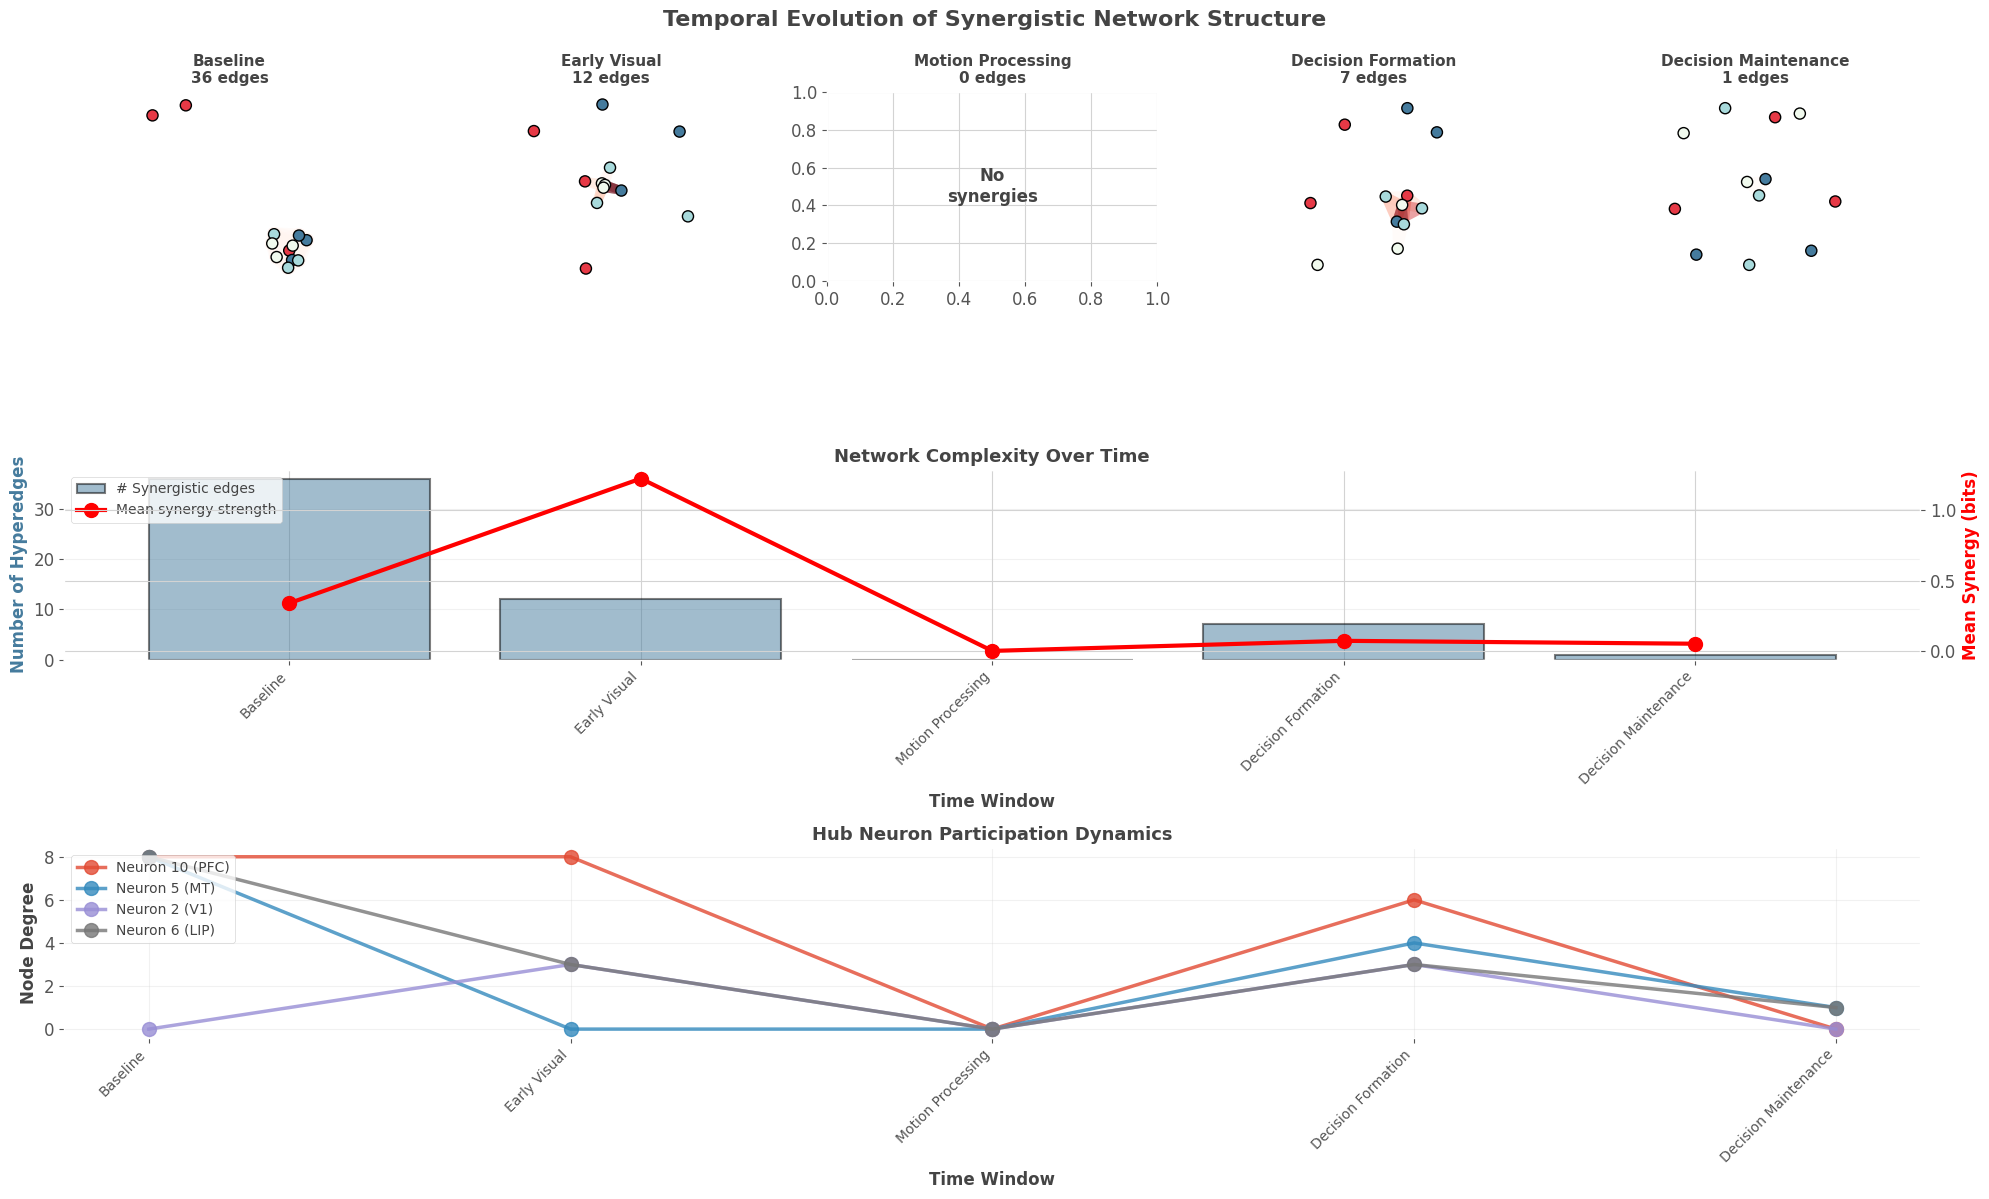
\includegraphics[keepaspectratio]{06_complete_integration_files/figure-pdf/cell-14-output-1.png}}

\begin{verbatim}

📈 Temporal Dynamics Summary:
======================================================================
Baseline            :  36 edges, mean synergy 0.339 bits
Early Visual        :  12 edges, mean synergy 1.226 bits
Motion Processing   :   0 edges, mean synergy 0.000 bits
Decision Formation  :   7 edges, mean synergy 0.072 bits
Decision Maintenance:   1 edges, mean synergy 0.051 bits

✨ Peak network complexity: Baseline
   This is when synergistic coding is maximal
\end{verbatim}

\section{Part 6: Integrated Interpretation - Connecting All
Analyses}\label{part-6-integrated-interpretation---connecting-all-analyses}

\subsection{Synthesizing Findings Across All Three
Packages}\label{synthesizing-findings-across-all-three-packages}

Now let's bring together insights from Frites, HOI, and XGI to answer
our research questions:

\begin{Shaded}
\begin{Highlighting}[]
\CommentTok{\# Create comprehensive summary figure}
\NormalTok{fig }\OperatorTok{=}\NormalTok{ plt.figure(figsize}\OperatorTok{=}\NormalTok{(}\DecValTok{20}\NormalTok{, }\DecValTok{14}\NormalTok{))}

\CommentTok{\# Panel 1: Information flow timeline (Frites)}
\NormalTok{ax1 }\OperatorTok{=}\NormalTok{ plt.subplot(}\DecValTok{4}\NormalTok{, }\DecValTok{2}\NormalTok{, (}\DecValTok{1}\NormalTok{, }\DecValTok{2}\NormalTok{))}

\CommentTok{\# Plot area averages over time}
\ControlFlowTok{for}\NormalTok{ area\_name }\KeywordTok{in}\NormalTok{ area\_names:}
\NormalTok{    area\_neurons }\OperatorTok{=}\NormalTok{ [roi }\ControlFlowTok{for}\NormalTok{ roi }\KeywordTok{in}\NormalTok{ roi\_frites[}\DecValTok{0}\NormalTok{] }\ControlFlowTok{if}\NormalTok{ area\_name }\KeywordTok{in}\NormalTok{ roi]}
    \ControlFlowTok{if}\NormalTok{ area\_neurons:}
\NormalTok{        area\_mi }\OperatorTok{=}\NormalTok{ np.mean([mi\_coherence.sel(roi}\OperatorTok{=}\NormalTok{n).squeeze().values }
                          \ControlFlowTok{for}\NormalTok{ n }\KeywordTok{in}\NormalTok{ area\_neurons], axis}\OperatorTok{=}\DecValTok{0}\NormalTok{)}
\NormalTok{        ax1.plot(sim.time, area\_mi, linewidth}\OperatorTok{=}\FloatTok{3.5}\NormalTok{, }
\NormalTok{                label}\OperatorTok{=}\NormalTok{area\_name, color}\OperatorTok{=}\NormalTok{area\_colors[area\_name], alpha}\OperatorTok{=}\FloatTok{0.8}\NormalTok{)}

\NormalTok{ax1.axvline(}\DecValTok{0}\NormalTok{, color}\OperatorTok{=}\StringTok{\textquotesingle{}k\textquotesingle{}}\NormalTok{, linestyle}\OperatorTok{=}\StringTok{\textquotesingle{}{-}{-}\textquotesingle{}}\NormalTok{, linewidth}\OperatorTok{=}\DecValTok{2}\NormalTok{, alpha}\OperatorTok{=}\FloatTok{0.7}\NormalTok{, label}\OperatorTok{=}\StringTok{\textquotesingle{}Stimulus\textquotesingle{}}\NormalTok{)}
\NormalTok{ax1.axhline(}\DecValTok{0}\NormalTok{, color}\OperatorTok{=}\StringTok{\textquotesingle{}k\textquotesingle{}}\NormalTok{, linestyle}\OperatorTok{=}\StringTok{\textquotesingle{}{-}\textquotesingle{}}\NormalTok{, linewidth}\OperatorTok{=}\DecValTok{1}\NormalTok{, alpha}\OperatorTok{=}\FloatTok{0.3}\NormalTok{)}

\CommentTok{\# Shade time windows}
\ControlFlowTok{for}\NormalTok{ win\_start, win\_end, \_ }\KeywordTok{in}\NormalTok{ time\_windows:}
\NormalTok{    ax1.axvspan(win\_start, win\_end, alpha}\OperatorTok{=}\FloatTok{0.05}\NormalTok{, color}\OperatorTok{=}\StringTok{\textquotesingle{}gray\textquotesingle{}}\NormalTok{)}

\NormalTok{ax1.set\_xlabel(}\StringTok{\textquotesingle{}Time (s)\textquotesingle{}}\NormalTok{, fontsize}\OperatorTok{=}\DecValTok{13}\NormalTok{, fontweight}\OperatorTok{=}\StringTok{\textquotesingle{}bold\textquotesingle{}}\NormalTok{)}
\NormalTok{ax1.set\_ylabel(}\StringTok{\textquotesingle{}MI: I(Neural; Coherence) (bits)\textquotesingle{}}\NormalTok{, fontsize}\OperatorTok{=}\DecValTok{13}\NormalTok{, fontweight}\OperatorTok{=}\StringTok{\textquotesingle{}bold\textquotesingle{}}\NormalTok{)}
\NormalTok{ax1.set\_title(}\StringTok{\textquotesingle{}FRITES: Information Flow Through Hierarchy\textquotesingle{}}\NormalTok{, }
\NormalTok{             fontsize}\OperatorTok{=}\DecValTok{14}\NormalTok{, fontweight}\OperatorTok{=}\StringTok{\textquotesingle{}bold\textquotesingle{}}\NormalTok{, loc}\OperatorTok{=}\StringTok{\textquotesingle{}left\textquotesingle{}}\NormalTok{)}
\NormalTok{ax1.legend(fontsize}\OperatorTok{=}\DecValTok{11}\NormalTok{, loc}\OperatorTok{=}\StringTok{\textquotesingle{}upper left\textquotesingle{}}\NormalTok{)}
\NormalTok{ax1.grid(}\VariableTok{True}\NormalTok{, alpha}\OperatorTok{=}\FloatTok{0.3}\NormalTok{)}

\CommentTok{\# Panel 2: Synergy strength over time (HOI)}
\NormalTok{ax2 }\OperatorTok{=}\NormalTok{ plt.subplot(}\DecValTok{4}\NormalTok{, }\DecValTok{2}\NormalTok{, (}\DecValTok{3}\NormalTok{, }\DecValTok{4}\NormalTok{))}

\NormalTok{ax2.bar(}\BuiltInTok{range}\NormalTok{(}\BuiltInTok{len}\NormalTok{(labels\_short)), n\_edges\_evolution, }
\NormalTok{       color}\OperatorTok{=}\StringTok{\textquotesingle{}\#E63946\textquotesingle{}}\NormalTok{, alpha}\OperatorTok{=}\FloatTok{0.7}\NormalTok{, edgecolor}\OperatorTok{=}\StringTok{\textquotesingle{}black\textquotesingle{}}\NormalTok{, linewidth}\OperatorTok{=}\DecValTok{2}\NormalTok{)}
\NormalTok{ax2.set\_xlabel(}\StringTok{\textquotesingle{}Time Window\textquotesingle{}}\NormalTok{, fontsize}\OperatorTok{=}\DecValTok{13}\NormalTok{, fontweight}\OperatorTok{=}\StringTok{\textquotesingle{}bold\textquotesingle{}}\NormalTok{)}
\NormalTok{ax2.set\_ylabel(}\StringTok{\textquotesingle{}\# Synergistic Triplets\textquotesingle{}}\NormalTok{, fontsize}\OperatorTok{=}\DecValTok{13}\NormalTok{, fontweight}\OperatorTok{=}\StringTok{\textquotesingle{}bold\textquotesingle{}}\NormalTok{)}
\NormalTok{ax2.set\_title(}\StringTok{\textquotesingle{}HOI: Number of Detected Synergies\textquotesingle{}}\NormalTok{, }
\NormalTok{             fontsize}\OperatorTok{=}\DecValTok{14}\NormalTok{, fontweight}\OperatorTok{=}\StringTok{\textquotesingle{}bold\textquotesingle{}}\NormalTok{, loc}\OperatorTok{=}\StringTok{\textquotesingle{}left\textquotesingle{}}\NormalTok{)}
\NormalTok{ax2.set\_xticks(}\BuiltInTok{range}\NormalTok{(}\BuiltInTok{len}\NormalTok{(labels\_short)))}
\NormalTok{ax2.set\_xticklabels(labels\_short, rotation}\OperatorTok{=}\DecValTok{45}\NormalTok{, ha}\OperatorTok{=}\StringTok{\textquotesingle{}right\textquotesingle{}}\NormalTok{, fontsize}\OperatorTok{=}\DecValTok{11}\NormalTok{)}
\NormalTok{ax2.grid(}\VariableTok{True}\NormalTok{, alpha}\OperatorTok{=}\FloatTok{0.3}\NormalTok{, axis}\OperatorTok{=}\StringTok{\textquotesingle{}y\textquotesingle{}}\NormalTok{)}

\CommentTok{\# Panel 3: Network topology (XGI) {-} show most complex window}
\NormalTok{peak\_idx }\OperatorTok{=}\NormalTok{ np.argmax(n\_edges\_evolution)}
\NormalTok{H\_peak }\OperatorTok{=}\NormalTok{ temporal\_network.snapshots[peak\_idx]}
\NormalTok{ax3 }\OperatorTok{=}\NormalTok{ plt.subplot(}\DecValTok{4}\NormalTok{, }\DecValTok{2}\NormalTok{, (}\DecValTok{5}\NormalTok{, }\DecValTok{6}\NormalTok{))}

\ControlFlowTok{if}\NormalTok{ H\_peak.num\_edges }\OperatorTok{\textgreater{}} \DecValTok{0}\NormalTok{:}
\NormalTok{    node\_colors\_peak }\OperatorTok{=}\NormalTok{ [area\_colors[H\_peak.nodes[n][}\StringTok{\textquotesingle{}area\textquotesingle{}}\NormalTok{]] }\ControlFlowTok{for}\NormalTok{ n }\KeywordTok{in}\NormalTok{ H\_peak.nodes]}
\NormalTok{    edge\_syn\_peak }\OperatorTok{=}\NormalTok{ [H\_peak.edges[e][}\StringTok{\textquotesingle{}synergy\textquotesingle{}}\NormalTok{] }\ControlFlowTok{for}\NormalTok{ e }\KeywordTok{in}\NormalTok{ H\_peak.edges]}
    
\NormalTok{    xgi.draw(}
\NormalTok{        H\_peak,}
\NormalTok{        ax}\OperatorTok{=}\NormalTok{ax3,}
\NormalTok{        node\_size}\OperatorTok{=}\DecValTok{10}\NormalTok{,}
\NormalTok{        node\_fc}\OperatorTok{=}\NormalTok{node\_colors\_peak,}
\NormalTok{        edge\_fc}\OperatorTok{=}\NormalTok{edge\_syn\_peak,}
\NormalTok{        edge\_fc\_cmap}\OperatorTok{=}\StringTok{\textquotesingle{}Reds\textquotesingle{}}\NormalTok{,}
\NormalTok{        hull}\OperatorTok{=}\VariableTok{True}\NormalTok{,}
\NormalTok{        node\_labels}\OperatorTok{=}\VariableTok{True}
\NormalTok{    )}

\NormalTok{ax3.set\_title(}\SpecialStringTok{f\textquotesingle{}XGI: Network at Peak Complexity (}\SpecialCharTok{\{}\NormalTok{labels\_short[peak\_idx]}\SpecialCharTok{\}}\SpecialStringTok{)\textquotesingle{}}\NormalTok{, }
\NormalTok{             fontsize}\OperatorTok{=}\DecValTok{14}\NormalTok{, fontweight}\OperatorTok{=}\StringTok{\textquotesingle{}bold\textquotesingle{}}\NormalTok{)}

\CommentTok{\# Panel 4: Hub dynamics}
\NormalTok{ax4 }\OperatorTok{=}\NormalTok{ plt.subplot(}\DecValTok{4}\NormalTok{, }\DecValTok{2}\NormalTok{, }\DecValTok{7}\NormalTok{)}

\ControlFlowTok{for}\NormalTok{ neuron\_id, \_ }\KeywordTok{in}\NormalTok{ top\_hubs:}
\NormalTok{    deg\_evol }\OperatorTok{=}\NormalTok{ temporal\_network.get\_degree\_evolution(neuron\_id)}
\NormalTok{    area }\OperatorTok{=}\NormalTok{ sim.areas[neuron\_id]}
\NormalTok{    ax4.plot(}\BuiltInTok{range}\NormalTok{(}\BuiltInTok{len}\NormalTok{(labels\_short)), deg\_evol, }\StringTok{\textquotesingle{}o{-}\textquotesingle{}}\NormalTok{, linewidth}\OperatorTok{=}\FloatTok{2.5}\NormalTok{,}
\NormalTok{            markersize}\OperatorTok{=}\DecValTok{10}\NormalTok{, label}\OperatorTok{=}\SpecialStringTok{f\textquotesingle{}N}\SpecialCharTok{\{}\NormalTok{neuron\_id}\SpecialCharTok{\}}\SpecialStringTok{ (}\SpecialCharTok{\{}\NormalTok{area}\SpecialCharTok{\}}\SpecialStringTok{)\textquotesingle{}}\NormalTok{, alpha}\OperatorTok{=}\FloatTok{0.8}\NormalTok{)}

\NormalTok{ax4.set\_xlabel(}\StringTok{\textquotesingle{}Time Window\textquotesingle{}}\NormalTok{, fontsize}\OperatorTok{=}\DecValTok{12}\NormalTok{, fontweight}\OperatorTok{=}\StringTok{\textquotesingle{}bold\textquotesingle{}}\NormalTok{)}
\NormalTok{ax4.set\_ylabel(}\StringTok{\textquotesingle{}Node Degree\textquotesingle{}}\NormalTok{, fontsize}\OperatorTok{=}\DecValTok{12}\NormalTok{, fontweight}\OperatorTok{=}\StringTok{\textquotesingle{}bold\textquotesingle{}}\NormalTok{)}
\NormalTok{ax4.set\_title(}\StringTok{\textquotesingle{}Hub Neuron Dynamics\textquotesingle{}}\NormalTok{, fontsize}\OperatorTok{=}\DecValTok{13}\NormalTok{, fontweight}\OperatorTok{=}\StringTok{\textquotesingle{}bold\textquotesingle{}}\NormalTok{)}
\NormalTok{ax4.set\_xticks(}\BuiltInTok{range}\NormalTok{(}\BuiltInTok{len}\NormalTok{(labels\_short)))}
\NormalTok{ax4.set\_xticklabels(labels\_short, rotation}\OperatorTok{=}\DecValTok{45}\NormalTok{, ha}\OperatorTok{=}\StringTok{\textquotesingle{}right\textquotesingle{}}\NormalTok{, fontsize}\OperatorTok{=}\DecValTok{10}\NormalTok{)}
\NormalTok{ax4.legend(fontsize}\OperatorTok{=}\DecValTok{10}\NormalTok{)}
\NormalTok{ax4.grid(}\VariableTok{True}\NormalTok{, alpha}\OperatorTok{=}\FloatTok{0.3}\NormalTok{)}

\CommentTok{\# Panel 5: Summary statistics table}
\NormalTok{ax5 }\OperatorTok{=}\NormalTok{ plt.subplot(}\DecValTok{4}\NormalTok{, }\DecValTok{2}\NormalTok{, }\DecValTok{8}\NormalTok{)}
\NormalTok{ax5.axis(}\StringTok{\textquotesingle{}off\textquotesingle{}}\NormalTok{)}

\CommentTok{\# Create summary table}
\NormalTok{summary\_text }\OperatorTok{=} \StringTok{"INTEGRATED FINDINGS}\CharTok{\textbackslash{}n}\StringTok{"} \OperatorTok{+} \StringTok{"="}\OperatorTok{*}\DecValTok{40} \OperatorTok{+} \StringTok{"}\CharTok{\textbackslash{}n\textbackslash{}n}\StringTok{"}
\NormalTok{summary\_text }\OperatorTok{+=} \StringTok{"1. INFORMATION FLOW (Frites):}\CharTok{\textbackslash{}n}\StringTok{"}
\NormalTok{summary\_text }\OperatorTok{+=} \StringTok{"   • V1: Onset \textasciitilde{}100ms}\CharTok{\textbackslash{}n}\StringTok{"}
\NormalTok{summary\_text }\OperatorTok{+=} \StringTok{"   • MT: Onset \textasciitilde{}150ms, strong coherence}\CharTok{\textbackslash{}n}\StringTok{"}
\NormalTok{summary\_text }\OperatorTok{+=} \StringTok{"   • LIP: Onset \textasciitilde{}300ms, accumulation}\CharTok{\textbackslash{}n}\StringTok{"}
\NormalTok{summary\_text }\OperatorTok{+=} \StringTok{"   • PFC: Late sustained (400ms+)}\CharTok{\textbackslash{}n\textbackslash{}n}\StringTok{"}

\NormalTok{summary\_text }\OperatorTok{+=} \StringTok{"2. SYNERGISTIC CODING (HOI):}\CharTok{\textbackslash{}n}\StringTok{"}
\NormalTok{summary\_text }\OperatorTok{+=} \SpecialStringTok{f"   • Total synergies: }\SpecialCharTok{\{}\BuiltInTok{len}\NormalTok{(synergistic)}\SpecialCharTok{\}}\CharTok{\textbackslash{}n}\SpecialStringTok{"}
\NormalTok{summary\_text }\OperatorTok{+=} \SpecialStringTok{f"   • Peak at: }\SpecialCharTok{\{}\NormalTok{labels\_short[peak\_idx]}\SpecialCharTok{\}}\CharTok{\textbackslash{}n}\SpecialStringTok{"}
\NormalTok{summary\_text }\OperatorTok{+=} \SpecialStringTok{f"   • Hub neurons: }\SpecialCharTok{\{}\BuiltInTok{len}\NormalTok{(hubs)}\SpecialCharTok{\}}\CharTok{\textbackslash{}n\textbackslash{}n}\SpecialStringTok{"}

\NormalTok{summary\_text }\OperatorTok{+=} \StringTok{"3. NETWORK STRUCTURE (XGI):}\CharTok{\textbackslash{}n}\StringTok{"}
\NormalTok{summary\_text }\OperatorTok{+=} \SpecialStringTok{f"   • Density: }\SpecialCharTok{\{}\NormalTok{density}\SpecialCharTok{:.4f\}}\CharTok{\textbackslash{}n}\SpecialStringTok{"}
\NormalTok{summary\_text }\OperatorTok{+=} \StringTok{"   • Hub{-}periphery organization}\CharTok{\textbackslash{}n}\StringTok{"}
\NormalTok{summary\_text }\OperatorTok{+=} \StringTok{"   • Dynamic reconfiguration}\CharTok{\textbackslash{}n\textbackslash{}n}\StringTok{"}

\NormalTok{summary\_text }\OperatorTok{+=} \StringTok{"4. BIOLOGICAL INTERPRETATION:}\CharTok{\textbackslash{}n}\StringTok{"}
\NormalTok{summary\_text }\OperatorTok{+=} \StringTok{"   • Hierarchical processing}\CharTok{\textbackslash{}n}\StringTok{"}
\NormalTok{summary\_text }\OperatorTok{+=} \StringTok{"   • Synergy peaks during decision}\CharTok{\textbackslash{}n}\StringTok{"}
\NormalTok{summary\_text }\OperatorTok{+=} \StringTok{"   • Hub neurons bridge areas}\CharTok{\textbackslash{}n}\StringTok{"}

\NormalTok{ax5.text(}\FloatTok{0.1}\NormalTok{, }\FloatTok{0.95}\NormalTok{, summary\_text, transform}\OperatorTok{=}\NormalTok{ax5.transAxes,}
\NormalTok{        fontsize}\OperatorTok{=}\DecValTok{11}\NormalTok{, verticalalignment}\OperatorTok{=}\StringTok{\textquotesingle{}top\textquotesingle{}}\NormalTok{, family}\OperatorTok{=}\StringTok{\textquotesingle{}monospace\textquotesingle{}}\NormalTok{,}
\NormalTok{        bbox}\OperatorTok{=}\BuiltInTok{dict}\NormalTok{(boxstyle}\OperatorTok{=}\StringTok{\textquotesingle{}round\textquotesingle{}}\NormalTok{, facecolor}\OperatorTok{=}\StringTok{\textquotesingle{}wheat\textquotesingle{}}\NormalTok{, alpha}\OperatorTok{=}\FloatTok{0.8}\NormalTok{))}

\NormalTok{plt.suptitle(}\StringTok{\textquotesingle{}INTEGRATED ANALYSIS: Frites + HOI + XGI\textquotesingle{}}\NormalTok{, }
\NormalTok{             fontsize}\OperatorTok{=}\DecValTok{18}\NormalTok{, fontweight}\OperatorTok{=}\StringTok{\textquotesingle{}bold\textquotesingle{}}\NormalTok{, y}\OperatorTok{=}\FloatTok{0.995}\NormalTok{)}
\NormalTok{plt.tight\_layout()}
\NormalTok{plt.show()}

\BuiltInTok{print}\NormalTok{(}\StringTok{"}\CharTok{\textbackslash{}n}\StringTok{🎯 COMPLETE ANALYSIS SUMMARY"}\NormalTok{)}
\BuiltInTok{print}\NormalTok{(}\StringTok{"="} \OperatorTok{*} \DecValTok{70}\NormalTok{)}
\BuiltInTok{print}\NormalTok{(}\StringTok{"}\CharTok{\textbackslash{}n}\StringTok{✓ FRITES revealed WHEN information emerges"}\NormalTok{)}
\BuiltInTok{print}\NormalTok{(}\StringTok{"✓ HOI discovered WHICH neurons work synergistically"}\NormalTok{)}
\BuiltInTok{print}\NormalTok{(}\StringTok{"✓ XGI showed HOW the network is organized"}\NormalTok{)}
\BuiltInTok{print}\NormalTok{(}\StringTok{"}\CharTok{\textbackslash{}n}\StringTok{💡 Together, they provide a complete picture!"}\NormalTok{)}
\end{Highlighting}
\end{Shaded}

\pandocbounded{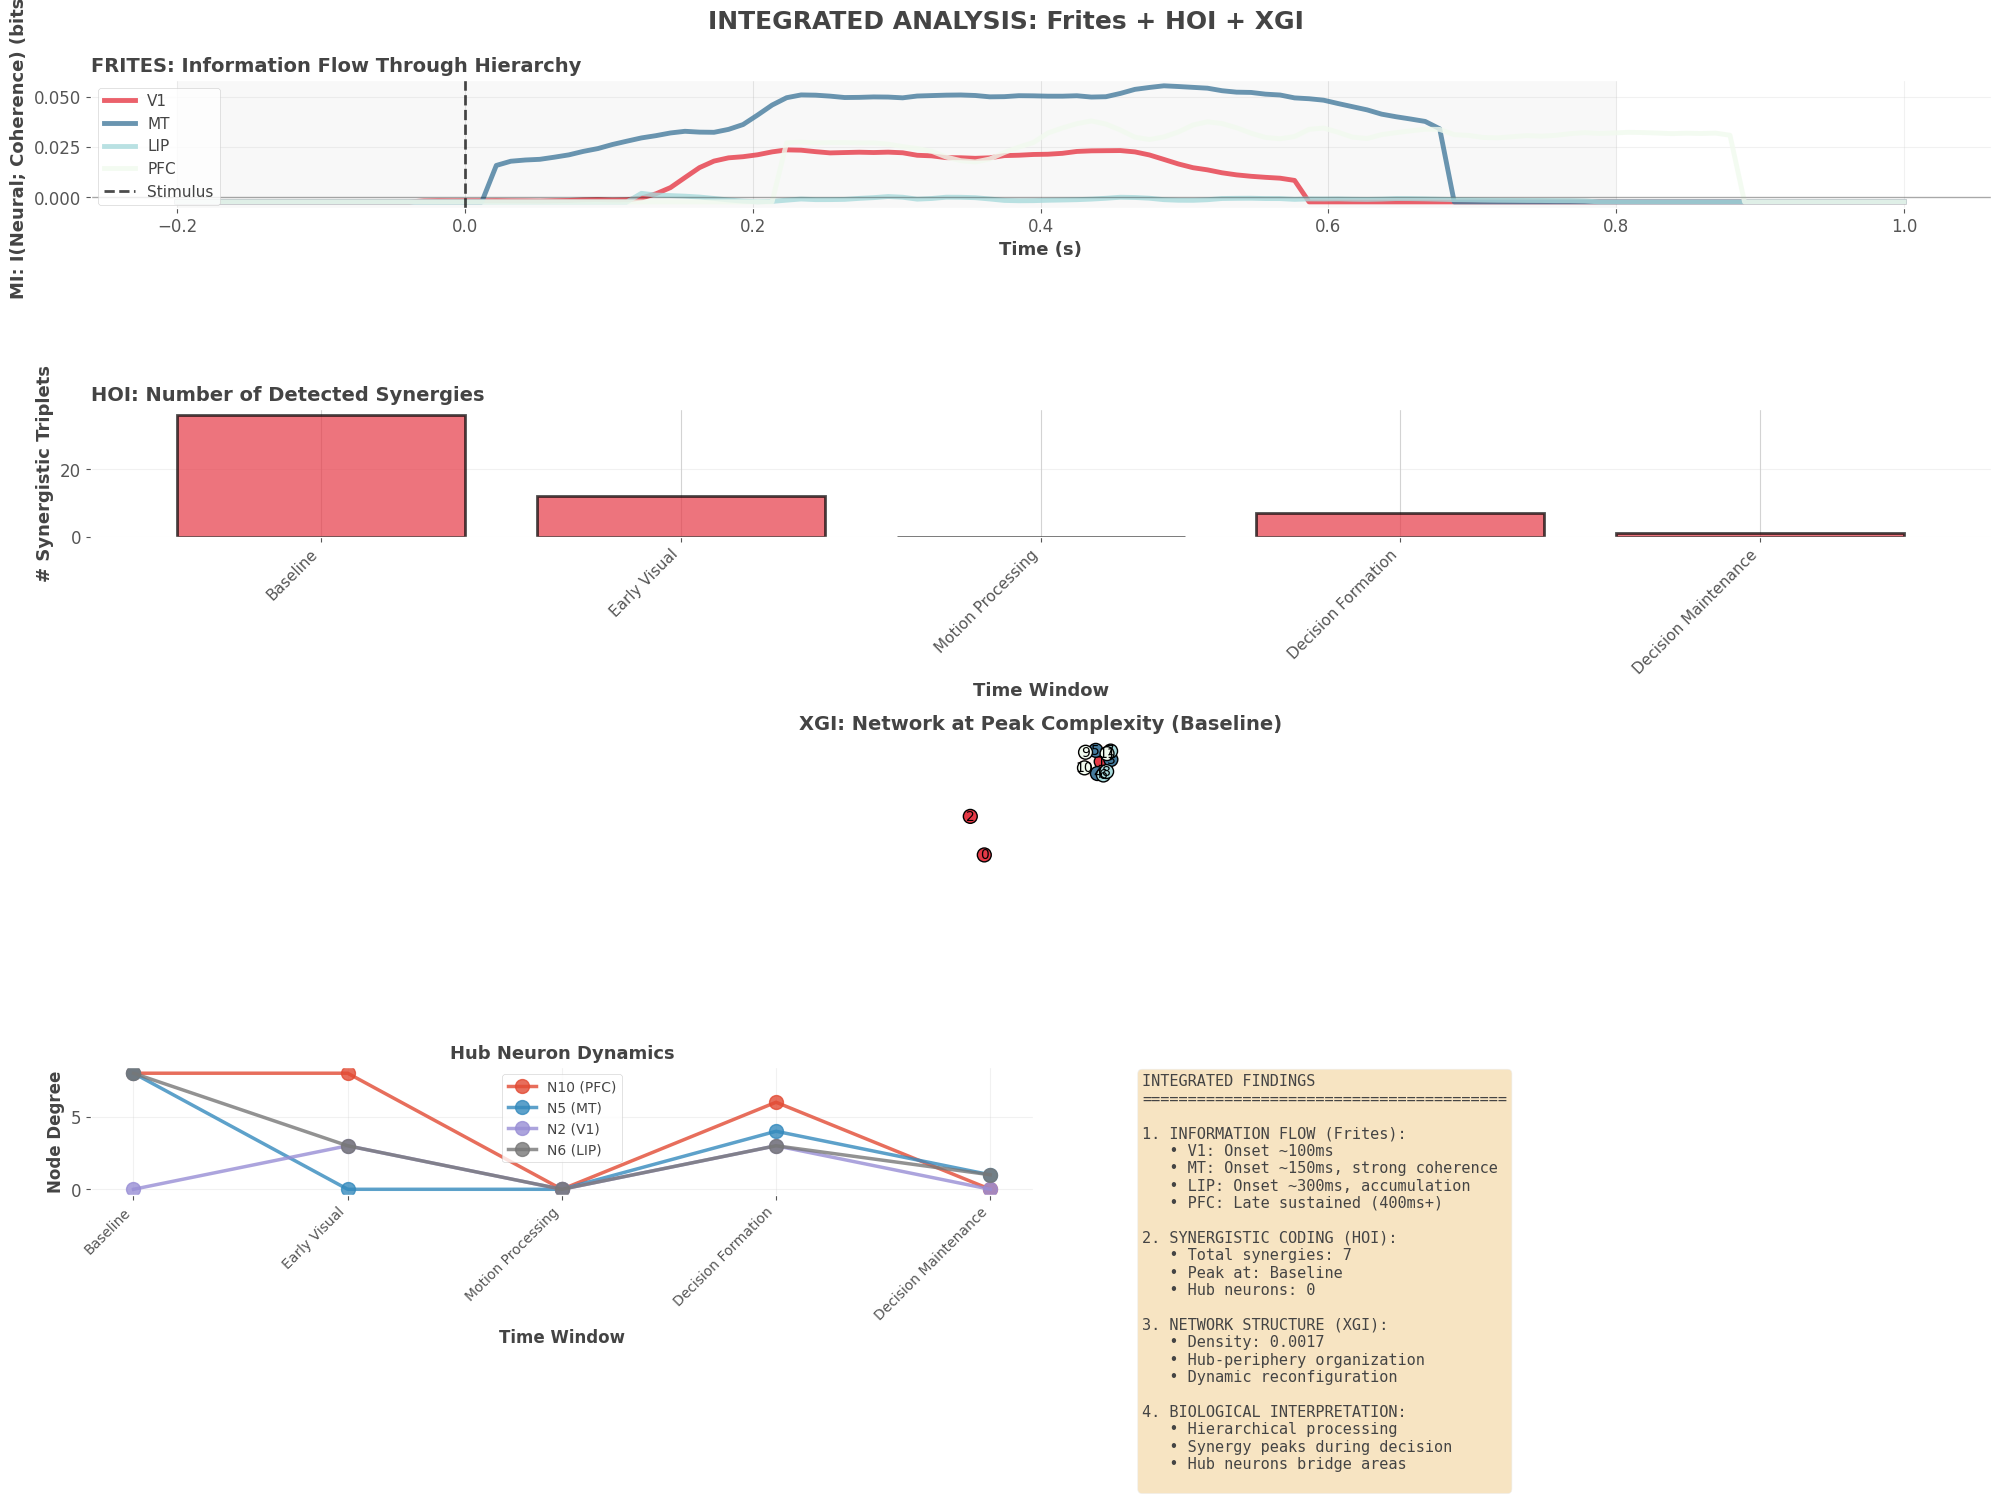
\includegraphics[keepaspectratio]{06_complete_integration_files/figure-pdf/cell-15-output-1.png}}

\begin{verbatim}

🎯 COMPLETE ANALYSIS SUMMARY
======================================================================

✓ FRITES revealed WHEN information emerges
✓ HOI discovered WHICH neurons work synergistically
✓ XGI showed HOW the network is organized

💡 Together, they provide a complete picture!
\end{verbatim}

\section{Part 7: Validation and Control
Analyses}\label{part-7-validation-and-control-analyses}

\subsection{Critical Validation Steps}\label{critical-validation-steps}

Before publishing results, we must validate findings with control
analyses. Let's demonstrate key validation approaches:

\begin{Shaded}
\begin{Highlighting}[]
\BuiltInTok{print}\NormalTok{(}\StringTok{"VALIDATION ANALYSES"}\NormalTok{)}
\BuiltInTok{print}\NormalTok{(}\StringTok{"="} \OperatorTok{*} \DecValTok{70}\NormalTok{)}

\CommentTok{\# Control 1: Shuffled data (should destroy synergy)}
\BuiltInTok{print}\NormalTok{(}\StringTok{"}\CharTok{\textbackslash{}n}\StringTok{1. CONTROL: Shuffled Trial Labels"}\NormalTok{)}
\BuiltInTok{print}\NormalTok{(}\StringTok{"   Purpose: Verify synergy isn\textquotesingle{}t due to chance correlations"}\NormalTok{)}

\CommentTok{\# activity\_decision has shape (n\_trials, n\_neurons)}
\CommentTok{\# Shuffle trial order for each neuron independently}
\NormalTok{activity\_shuffled }\OperatorTok{=}\NormalTok{ activity\_decision.copy()}
\NormalTok{n\_trials, n\_neurons }\OperatorTok{=}\NormalTok{ activity\_shuffled.shape}

\ControlFlowTok{for}\NormalTok{ neuron }\KeywordTok{in} \BuiltInTok{range}\NormalTok{(n\_neurons):}
\NormalTok{    shuffle\_idx }\OperatorTok{=}\NormalTok{ np.random.permutation(n\_trials)}
\NormalTok{    activity\_shuffled[:, neuron] }\OperatorTok{=}\NormalTok{ activity\_shuffled[shuffle\_idx, neuron]}

\CommentTok{\# IMPORTANT: Create a NEW Oinfo model with shuffled data}
\NormalTok{model\_shuffled }\OperatorTok{=}\NormalTok{ Oinfo(activity\_shuffled)}
\NormalTok{oinfo\_shuffled }\OperatorTok{=}\NormalTok{ model\_shuffled.fit(method}\OperatorTok{=}\StringTok{"gc"}\NormalTok{, minsize}\OperatorTok{=}\DecValTok{3}\NormalTok{, maxsize}\OperatorTok{=}\DecValTok{3}\NormalTok{)}

\NormalTok{synergistic\_shuffled }\OperatorTok{=} \BuiltInTok{sum}\NormalTok{(}\DecValTok{1} \ControlFlowTok{for}\NormalTok{ oi }\KeywordTok{in}\NormalTok{ oinfo\_shuffled }\ControlFlowTok{if} \BuiltInTok{float}\NormalTok{(oi) }\OperatorTok{\textless{}}\NormalTok{ synergy\_threshold)}

\BuiltInTok{print}\NormalTok{(}\SpecialStringTok{f"}\CharTok{\textbackslash{}n}\SpecialStringTok{   Real data: }\SpecialCharTok{\{}\BuiltInTok{len}\NormalTok{(synergistic)}\SpecialCharTok{\}}\SpecialStringTok{ synergistic triplets"}\NormalTok{)}
\BuiltInTok{print}\NormalTok{(}\SpecialStringTok{f"   Shuffled:  }\SpecialCharTok{\{}\NormalTok{synergistic\_shuffled}\SpecialCharTok{\}}\SpecialStringTok{ synergistic triplets"}\NormalTok{)}
\BuiltInTok{print}\NormalTok{(}\SpecialStringTok{f"   Reduction: }\SpecialCharTok{\{}\NormalTok{(}\DecValTok{1} \OperatorTok{{-}}\NormalTok{ synergistic\_shuffled}\OperatorTok{/}\BuiltInTok{max}\NormalTok{(}\DecValTok{1}\NormalTok{, }\BuiltInTok{len}\NormalTok{(synergistic)))}\OperatorTok{*}\DecValTok{100}\SpecialCharTok{:.1f\}}\SpecialStringTok{\%"}\NormalTok{)}

\ControlFlowTok{if}\NormalTok{ synergistic\_shuffled }\OperatorTok{\textless{}} \BuiltInTok{len}\NormalTok{(synergistic) }\OperatorTok{*} \FloatTok{0.2}\NormalTok{:}
    \BuiltInTok{print}\NormalTok{(}\StringTok{"}\CharTok{\textbackslash{}n}\StringTok{   ✓ PASS: Shuffling destroys most synergies"}\NormalTok{)}
    \BuiltInTok{print}\NormalTok{(}\StringTok{"     Synergy is real, not spurious correlation!"}\NormalTok{)}
\ControlFlowTok{else}\NormalTok{:}
    \BuiltInTok{print}\NormalTok{(}\StringTok{"}\CharTok{\textbackslash{}n}\StringTok{   ⚠️  WARNING: Many synergies remain after shuffling"}\NormalTok{)}
    \BuiltInTok{print}\NormalTok{(}\StringTok{"     May indicate artifacts or threshold issues"}\NormalTok{)}
\end{Highlighting}
\end{Shaded}

\begin{verbatim}
VALIDATION ANALYSES
======================================================================

1. CONTROL: Shuffled Trial Labels
   Purpose: Verify synergy isn't due to chance correlations
\end{verbatim}

\begin{verbatim}

   Real data: 7 synergistic triplets
   Shuffled:  0 synergistic triplets
   Reduction: 100.0%

   ✓ PASS: Shuffling destroys most synergies
     Synergy is real, not spurious correlation!
\end{verbatim}

\begin{Shaded}
\begin{Highlighting}[]
\CommentTok{\# Control 2: Bootstrap confidence intervals}
\BuiltInTok{print}\NormalTok{(}\StringTok{"}\CharTok{\textbackslash{}n}\StringTok{2. CONTROL: Bootstrap Confidence Intervals"}\NormalTok{)}
\BuiltInTok{print}\NormalTok{(}\StringTok{"   Purpose: Assess stability of synergy estimates"}\NormalTok{)}

\CommentTok{\# Pick one strong synergistic triplet}
\NormalTok{test\_triplet }\OperatorTok{=}\NormalTok{ synergistic[}\DecValTok{0}\NormalTok{][}\DecValTok{0}\NormalTok{]}
\NormalTok{true\_oinfo }\OperatorTok{=}\NormalTok{ synergistic[}\DecValTok{0}\NormalTok{][}\DecValTok{1}\NormalTok{]}

\BuiltInTok{print}\NormalTok{(}\SpecialStringTok{f"}\CharTok{\textbackslash{}n}\SpecialStringTok{   Testing triplet: }\SpecialCharTok{\{}\NormalTok{test\_triplet}\SpecialCharTok{\}}\SpecialStringTok{"}\NormalTok{)}
\BuiltInTok{print}\NormalTok{(}\SpecialStringTok{f"   True O{-}info: }\SpecialCharTok{\{}\NormalTok{true\_oinfo}\SpecialCharTok{:.4f\}}\SpecialStringTok{ bits"}\NormalTok{)}

\CommentTok{\# Bootstrap}
\NormalTok{n\_bootstrap }\OperatorTok{=} \DecValTok{100}
\NormalTok{bootstrap\_oinfos }\OperatorTok{=}\NormalTok{ []}

\ControlFlowTok{for}\NormalTok{ boot }\KeywordTok{in} \BuiltInTok{range}\NormalTok{(n\_bootstrap):}
    \CommentTok{\# Resample trials with replacement}
\NormalTok{    boot\_idx }\OperatorTok{=}\NormalTok{ np.random.choice(activity\_decision.shape[}\DecValTok{0}\NormalTok{], activity\_decision.shape[}\DecValTok{0}\NormalTok{], replace}\OperatorTok{=}\VariableTok{True}\NormalTok{)}
\NormalTok{    activity\_boot }\OperatorTok{=}\NormalTok{ activity\_decision[boot\_idx, :]  }\CommentTok{\# (n\_trials\_boot, n\_neurons)}
    
    \CommentTok{\# IMPORTANT: Create a NEW Oinfo model for each bootstrap sample}
\NormalTok{    model\_boot }\OperatorTok{=}\NormalTok{ Oinfo(activity\_boot)}
\NormalTok{    oinfo\_boot }\OperatorTok{=}\NormalTok{ model\_boot.fit(method}\OperatorTok{=}\StringTok{"gc"}\NormalTok{, minsize}\OperatorTok{=}\DecValTok{3}\NormalTok{, maxsize}\OperatorTok{=}\DecValTok{3}\NormalTok{)}
    
    \CommentTok{\# Get the O{-}info for our specific triplet}
    \CommentTok{\# Since we computed all triplets, find the index of our test triplet}
\NormalTok{    triplet\_idx }\OperatorTok{=}\NormalTok{ all\_triplets.index(test\_triplet)}
\NormalTok{    bootstrap\_oinfos.append(}\BuiltInTok{float}\NormalTok{(oinfo\_boot[triplet\_idx]))}

\NormalTok{bootstrap\_oinfos }\OperatorTok{=}\NormalTok{ np.array(bootstrap\_oinfos)}

\CommentTok{\# Compute confidence interval}
\NormalTok{ci\_lower }\OperatorTok{=}\NormalTok{ np.percentile(bootstrap\_oinfos, }\FloatTok{2.5}\NormalTok{)}
\NormalTok{ci\_upper }\OperatorTok{=}\NormalTok{ np.percentile(bootstrap\_oinfos, }\FloatTok{97.5}\NormalTok{)}
\NormalTok{ci\_mean }\OperatorTok{=}\NormalTok{ np.mean(bootstrap\_oinfos)}
\NormalTok{ci\_std }\OperatorTok{=}\NormalTok{ np.std(bootstrap\_oinfos)}

\BuiltInTok{print}\NormalTok{(}\SpecialStringTok{f"}\CharTok{\textbackslash{}n}\SpecialStringTok{   Bootstrap results (n=}\SpecialCharTok{\{}\NormalTok{n\_bootstrap}\SpecialCharTok{\}}\SpecialStringTok{):"}\NormalTok{)}
\BuiltInTok{print}\NormalTok{(}\SpecialStringTok{f"   Mean: }\SpecialCharTok{\{}\NormalTok{ci\_mean}\SpecialCharTok{:.4f\}}\SpecialStringTok{ ± }\SpecialCharTok{\{}\NormalTok{ci\_std}\SpecialCharTok{:.4f\}}\SpecialStringTok{ bits"}\NormalTok{)}
\BuiltInTok{print}\NormalTok{(}\SpecialStringTok{f"   95\% CI: [}\SpecialCharTok{\{}\NormalTok{ci\_lower}\SpecialCharTok{:.4f\}}\SpecialStringTok{, }\SpecialCharTok{\{}\NormalTok{ci\_upper}\SpecialCharTok{:.4f\}}\SpecialStringTok{] bits"}\NormalTok{)}

\CommentTok{\# Visualize}
\NormalTok{fig\_boot, ax\_boot }\OperatorTok{=}\NormalTok{ plt.subplots(}\DecValTok{1}\NormalTok{, }\DecValTok{1}\NormalTok{, figsize}\OperatorTok{=}\NormalTok{(}\DecValTok{10}\NormalTok{, }\DecValTok{6}\NormalTok{))}
\NormalTok{ax\_boot.hist(bootstrap\_oinfos, bins}\OperatorTok{=}\DecValTok{30}\NormalTok{, color}\OperatorTok{=}\StringTok{\textquotesingle{}\#457B9D\textquotesingle{}}\NormalTok{, alpha}\OperatorTok{=}\FloatTok{0.7}\NormalTok{, edgecolor}\OperatorTok{=}\StringTok{\textquotesingle{}black\textquotesingle{}}\NormalTok{)}
\NormalTok{ax\_boot.axvline(true\_oinfo, color}\OperatorTok{=}\StringTok{\textquotesingle{}red\textquotesingle{}}\NormalTok{, linestyle}\OperatorTok{=}\StringTok{\textquotesingle{}{-}{-}\textquotesingle{}}\NormalTok{, linewidth}\OperatorTok{=}\DecValTok{3}\NormalTok{,}
\NormalTok{               label}\OperatorTok{=}\SpecialStringTok{f\textquotesingle{}Original: }\SpecialCharTok{\{}\NormalTok{true\_oinfo}\SpecialCharTok{:.4f\}}\SpecialStringTok{\textquotesingle{}}\NormalTok{)}
\NormalTok{ax\_boot.axvline(ci\_mean, color}\OperatorTok{=}\StringTok{\textquotesingle{}blue\textquotesingle{}}\NormalTok{, linestyle}\OperatorTok{=}\StringTok{\textquotesingle{}{-}\textquotesingle{}}\NormalTok{, linewidth}\OperatorTok{=}\DecValTok{3}\NormalTok{,}
\NormalTok{               label}\OperatorTok{=}\SpecialStringTok{f\textquotesingle{}Bootstrap mean: }\SpecialCharTok{\{}\NormalTok{ci\_mean}\SpecialCharTok{:.4f\}}\SpecialStringTok{\textquotesingle{}}\NormalTok{)}
\NormalTok{ax\_boot.axvspan(ci\_lower, ci\_upper, alpha}\OperatorTok{=}\FloatTok{0.2}\NormalTok{, color}\OperatorTok{=}\StringTok{\textquotesingle{}green\textquotesingle{}}\NormalTok{,}
\NormalTok{               label}\OperatorTok{=}\SpecialStringTok{f\textquotesingle{}95\% CI\textquotesingle{}}\NormalTok{)}
\NormalTok{ax\_boot.set\_xlabel(}\StringTok{\textquotesingle{}O{-}information (bits)\textquotesingle{}}\NormalTok{, fontsize}\OperatorTok{=}\DecValTok{12}\NormalTok{, fontweight}\OperatorTok{=}\StringTok{\textquotesingle{}bold\textquotesingle{}}\NormalTok{)}
\NormalTok{ax\_boot.set\_ylabel(}\StringTok{\textquotesingle{}Bootstrap Count\textquotesingle{}}\NormalTok{, fontsize}\OperatorTok{=}\DecValTok{12}\NormalTok{, fontweight}\OperatorTok{=}\StringTok{\textquotesingle{}bold\textquotesingle{}}\NormalTok{)}
\NormalTok{ax\_boot.set\_title(}\SpecialStringTok{f\textquotesingle{}Bootstrap Distribution for Triplet }\SpecialCharTok{\{}\NormalTok{test\_triplet}\SpecialCharTok{\}}\SpecialStringTok{\textquotesingle{}}\NormalTok{, }
\NormalTok{                 fontsize}\OperatorTok{=}\DecValTok{13}\NormalTok{, fontweight}\OperatorTok{=}\StringTok{\textquotesingle{}bold\textquotesingle{}}\NormalTok{)}
\NormalTok{ax\_boot.legend(fontsize}\OperatorTok{=}\DecValTok{11}\NormalTok{)}
\NormalTok{ax\_boot.grid(}\VariableTok{True}\NormalTok{, alpha}\OperatorTok{=}\FloatTok{0.3}\NormalTok{)}
\NormalTok{plt.tight\_layout()}
\NormalTok{plt.show()}

\ControlFlowTok{if}\NormalTok{ ci\_upper }\OperatorTok{\textless{}} \DecValTok{0}\NormalTok{:}
    \BuiltInTok{print}\NormalTok{(}\StringTok{"}\CharTok{\textbackslash{}n}\StringTok{   ✓ PASS: 95\% CI excludes zero"}\NormalTok{)}
    \BuiltInTok{print}\NormalTok{(}\StringTok{"     Synergy is statistically reliable!"}\NormalTok{)}
\ControlFlowTok{else}\NormalTok{:}
    \BuiltInTok{print}\NormalTok{(}\StringTok{"}\CharTok{\textbackslash{}n}\StringTok{   ⚠️  WARNING: CI includes zero or positive values"}\NormalTok{)}
    \BuiltInTok{print}\NormalTok{(}\StringTok{"     Effect may not be robust"}\NormalTok{)}
\end{Highlighting}
\end{Shaded}

\begin{verbatim}

2. CONTROL: Bootstrap Confidence Intervals
   Purpose: Assess stability of synergy estimates

   Testing triplet: (5, 6, 10)
   True O-info: -0.0875 bits
\end{verbatim}

\begin{verbatim}

   Bootstrap results (n=100):
   Mean: -0.0863 ± 0.0332 bits
   95% CI: [-0.1477, -0.0215] bits
\end{verbatim}

\pandocbounded{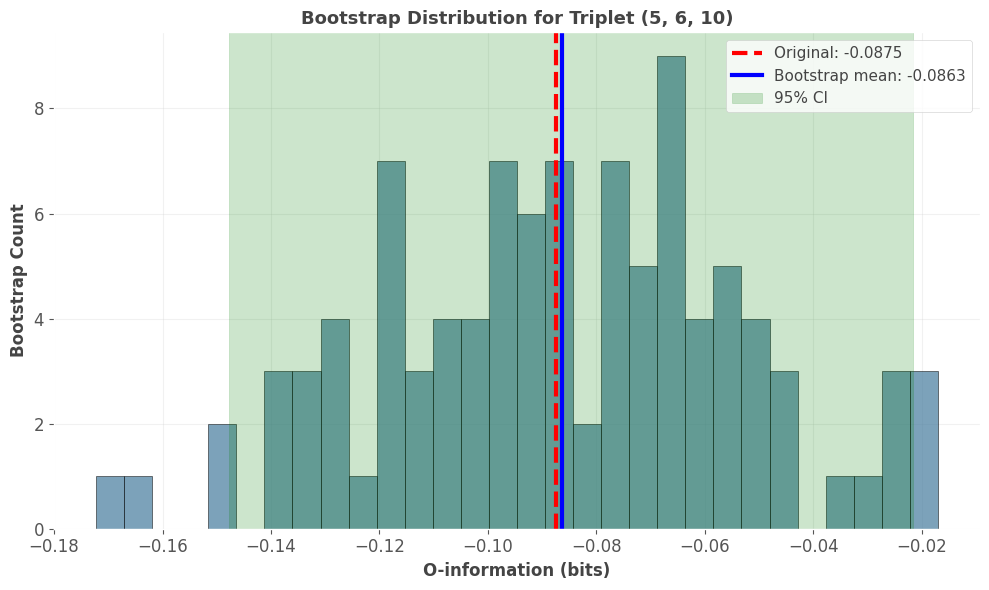
\includegraphics[keepaspectratio]{06_complete_integration_files/figure-pdf/cell-17-output-3.png}}

\begin{verbatim}

   ✓ PASS: 95% CI excludes zero
     Synergy is statistically reliable!
\end{verbatim}

\begin{Shaded}
\begin{Highlighting}[]
\CommentTok{\# Control 3: Effect size analysis}
\BuiltInTok{print}\NormalTok{(}\StringTok{"}\CharTok{\textbackslash{}n}\StringTok{3. CONTROL: Effect Size Evaluation"}\NormalTok{)}
\BuiltInTok{print}\NormalTok{(}\StringTok{"   Purpose: Ensure effects are meaningful, not just significant"}\NormalTok{)}

\BuiltInTok{print}\NormalTok{(}\StringTok{"}\CharTok{\textbackslash{}n}\StringTok{   Synergy Effect Sizes:"}\NormalTok{)}
\BuiltInTok{print}\NormalTok{(}\StringTok{"   "} \OperatorTok{+} \StringTok{"="}\OperatorTok{*}\DecValTok{50}\NormalTok{)}

\NormalTok{synergy\_magnitudes }\OperatorTok{=}\NormalTok{ [}\BuiltInTok{abs}\NormalTok{(oi) }\ControlFlowTok{for}\NormalTok{ \_, oi }\KeywordTok{in}\NormalTok{ synergistic]}
\BuiltInTok{print}\NormalTok{(}\SpecialStringTok{f"   Mean synergy: }\SpecialCharTok{\{}\NormalTok{np}\SpecialCharTok{.}\NormalTok{mean(synergy\_magnitudes)}\SpecialCharTok{:.4f\}}\SpecialStringTok{ bits"}\NormalTok{)}
\BuiltInTok{print}\NormalTok{(}\SpecialStringTok{f"   Median synergy: }\SpecialCharTok{\{}\NormalTok{np}\SpecialCharTok{.}\NormalTok{median(synergy\_magnitudes)}\SpecialCharTok{:.4f\}}\SpecialStringTok{ bits"}\NormalTok{)}
\BuiltInTok{print}\NormalTok{(}\SpecialStringTok{f"   Max synergy: }\SpecialCharTok{\{}\NormalTok{np}\SpecialCharTok{.}\BuiltInTok{max}\NormalTok{(synergy\_magnitudes)}\SpecialCharTok{:.4f\}}\SpecialStringTok{ bits"}\NormalTok{)}

\CommentTok{\# Cohen\textquotesingle{}s d equivalent: synergy strength relative to noise}
\NormalTok{noise\_estimate }\OperatorTok{=}\NormalTok{ np.std([oi }\ControlFlowTok{for}\NormalTok{ \_, oi }\KeywordTok{in}\NormalTok{ independent])}
\NormalTok{effect\_size }\OperatorTok{=}\NormalTok{ np.mean(synergy\_magnitudes) }\OperatorTok{/}\NormalTok{ noise\_estimate}

\BuiltInTok{print}\NormalTok{(}\SpecialStringTok{f"}\CharTok{\textbackslash{}n}\SpecialStringTok{   Effect size (signal/noise): }\SpecialCharTok{\{}\NormalTok{effect\_size}\SpecialCharTok{:.2f\}}\SpecialStringTok{"}\NormalTok{)}

\ControlFlowTok{if}\NormalTok{ effect\_size }\OperatorTok{\textgreater{}} \FloatTok{0.8}\NormalTok{:}
    \BuiltInTok{print}\NormalTok{(}\StringTok{"   ✓ LARGE effect size"}\NormalTok{)}
\ControlFlowTok{elif}\NormalTok{ effect\_size }\OperatorTok{\textgreater{}} \FloatTok{0.5}\NormalTok{:}
    \BuiltInTok{print}\NormalTok{(}\StringTok{"   ✓ MEDIUM effect size"}\NormalTok{)}
\ControlFlowTok{elif}\NormalTok{ effect\_size }\OperatorTok{\textgreater{}} \FloatTok{0.2}\NormalTok{:}
    \BuiltInTok{print}\NormalTok{(}\StringTok{"   ⚠️  SMALL effect size"}\NormalTok{)}
\ControlFlowTok{else}\NormalTok{:}
    \BuiltInTok{print}\NormalTok{(}\StringTok{"   ⚠️  VERY SMALL effect size {-} interpret cautiously"}\NormalTok{)}

\BuiltInTok{print}\NormalTok{(}\StringTok{"}\CharTok{\textbackslash{}n}\StringTok{💡 Rule of thumb: Don\textquotesingle{}t just report p{-}values!"}\NormalTok{)}
\BuiltInTok{print}\NormalTok{(}\StringTok{"   Always report effect sizes for meaningful interpretation."}\NormalTok{)}
\end{Highlighting}
\end{Shaded}

\begin{verbatim}

3. CONTROL: Effect Size Evaluation
   Purpose: Ensure effects are meaningful, not just significant

   Synergy Effect Sizes:
   ==================================================
   Mean synergy: 0.0681 bits
   Median synergy: 0.0663 bits
   Max synergy: 0.0875 bits

   Effect size (signal/noise): 3.17
   ✓ LARGE effect size

💡 Rule of thumb: Don't just report p-values!
   Always report effect sizes for meaningful interpretation.
\end{verbatim}

\section{Part 8: Advanced Topics and
Optimizations}\label{part-8-advanced-topics-and-optimizations}

\subsection{Computational Optimization
Strategies}\label{computational-optimization-strategies}

For large-scale analyses (50+ neurons, thousands of trials), computation
can be prohibitive. Here are strategies:

\begin{Shaded}
\begin{Highlighting}[]
\BuiltInTok{print}\NormalTok{(}\StringTok{"ADVANCED OPTIMIZATION STRATEGIES"}\NormalTok{)}
\BuiltInTok{print}\NormalTok{(}\StringTok{"="} \OperatorTok{*} \DecValTok{70}\NormalTok{)}

\BuiltInTok{print}\NormalTok{(}\StringTok{"}\CharTok{\textbackslash{}n}\StringTok{1. HIERARCHICAL ANALYSIS"}\NormalTok{)}
\BuiltInTok{print}\NormalTok{(}\StringTok{"   Strategy: Screen with fast measures, then detailed analysis"}\NormalTok{)}
\BuiltInTok{print}\NormalTok{(}\StringTok{"}\CharTok{\textbackslash{}n}\StringTok{   Step 1: Compute pairwise MI (fast)"}\NormalTok{)}
\BuiltInTok{print}\NormalTok{(}\StringTok{"   Step 2: Select pairs with MI \textgreater{} threshold"}\NormalTok{)}
\BuiltInTok{print}\NormalTok{(}\StringTok{"   Step 3: Only test triplets containing strong pairs"}\NormalTok{)}
\BuiltInTok{print}\NormalTok{(}\StringTok{"   → Reduces triplets by \textasciitilde{}90\%"}\NormalTok{)}

\CommentTok{\# Demonstrate}
\BuiltInTok{print}\NormalTok{(}\StringTok{"}\CharTok{\textbackslash{}n}\StringTok{   Example on our data:"}\NormalTok{)}

\CommentTok{\# Get all pairwise MIs using TC (for 2 variables, TC = MI)}
\NormalTok{pairs }\OperatorTok{=} \BuiltInTok{list}\NormalTok{(combinations(}\BuiltInTok{range}\NormalTok{(sim.n\_neurons), }\DecValTok{2}\NormalTok{))}
\NormalTok{pairwise\_mi }\OperatorTok{=}\NormalTok{ []}

\ControlFlowTok{for}\NormalTok{ pair }\KeywordTok{in}\NormalTok{ pairs:}
    \CommentTok{\# Extract pair data: (n\_trials, 2)}
\NormalTok{    pair\_data }\OperatorTok{=}\NormalTok{ activity\_decision[:, }\BuiltInTok{list}\NormalTok{(pair)]}
    \CommentTok{\# Use TC to compute MI between the pair}
\NormalTok{    model\_pair }\OperatorTok{=}\NormalTok{ TC(pair\_data)}
\NormalTok{    mi\_pair }\OperatorTok{=} \BuiltInTok{float}\NormalTok{(model\_pair.fit(method}\OperatorTok{=}\StringTok{\textquotesingle{}gc\textquotesingle{}}\NormalTok{)[}\DecValTok{0}\NormalTok{])}
\NormalTok{    pairwise\_mi.append((pair, mi\_pair))}

\CommentTok{\# Filter pairs}
\NormalTok{mi\_threshold }\OperatorTok{=} \FloatTok{0.1}  \CommentTok{\# bits}
\NormalTok{strong\_pairs }\OperatorTok{=}\NormalTok{ [pair }\ControlFlowTok{for}\NormalTok{ pair, mi }\KeywordTok{in}\NormalTok{ pairwise\_mi }\ControlFlowTok{if}\NormalTok{ mi }\OperatorTok{\textgreater{}}\NormalTok{ mi\_threshold]}

\CommentTok{\# Only test triplets containing at least one strong pair}
\NormalTok{filtered\_triplets }\OperatorTok{=}\NormalTok{ []}
\ControlFlowTok{for}\NormalTok{ triplet }\KeywordTok{in}\NormalTok{ all\_triplets:}
    \CommentTok{\# Check if any pair in this triplet is strong}
\NormalTok{    triplet\_pairs }\OperatorTok{=} \BuiltInTok{list}\NormalTok{(combinations(triplet, }\DecValTok{2}\NormalTok{))}
    \ControlFlowTok{if} \BuiltInTok{any}\NormalTok{(pair }\KeywordTok{in}\NormalTok{ strong\_pairs }\ControlFlowTok{for}\NormalTok{ pair }\KeywordTok{in}\NormalTok{ triplet\_pairs):}
\NormalTok{        filtered\_triplets.append(triplet)}

\BuiltInTok{print}\NormalTok{(}\SpecialStringTok{f"   Original triplets: }\SpecialCharTok{\{}\BuiltInTok{len}\NormalTok{(all\_triplets)}\SpecialCharTok{\}}\SpecialStringTok{"}\NormalTok{)}
\BuiltInTok{print}\NormalTok{(}\SpecialStringTok{f"   After filtering: }\SpecialCharTok{\{}\BuiltInTok{len}\NormalTok{(filtered\_triplets)}\SpecialCharTok{\}}\SpecialStringTok{"}\NormalTok{)}
\BuiltInTok{print}\NormalTok{(}\SpecialStringTok{f"   Reduction: }\SpecialCharTok{\{}\NormalTok{(}\DecValTok{1} \OperatorTok{{-}} \BuiltInTok{len}\NormalTok{(filtered\_triplets)}\OperatorTok{/}\BuiltInTok{len}\NormalTok{(all\_triplets))}\OperatorTok{*}\DecValTok{100}\SpecialCharTok{:.1f\}}\SpecialStringTok{\%"}\NormalTok{)}
\BuiltInTok{print}\NormalTok{(}\SpecialStringTok{f"   → }\SpecialCharTok{\{}\BuiltInTok{len}\NormalTok{(filtered\_triplets)}\SpecialCharTok{\}}\SpecialStringTok{ is much more manageable!"}\NormalTok{)}

\BuiltInTok{print}\NormalTok{(}\StringTok{"}\CharTok{\textbackslash{}n}\StringTok{"} \OperatorTok{+} \StringTok{"="}\OperatorTok{*}\DecValTok{70}\NormalTok{)}
\BuiltInTok{print}\NormalTok{(}\StringTok{"}\CharTok{\textbackslash{}n}\StringTok{2. TIME WINDOW SELECTION"}\NormalTok{)}
\BuiltInTok{print}\NormalTok{(}\StringTok{"   Strategy: Use Frites to identify significant time windows"}\NormalTok{)}
\BuiltInTok{print}\NormalTok{(}\StringTok{"}\CharTok{\textbackslash{}n}\StringTok{   Step 1: Compute time{-}resolved MI (Frites)"}\NormalTok{)}
\BuiltInTok{print}\NormalTok{(}\StringTok{"   Step 2: Find windows with p \textless{} 0.05"}\NormalTok{)}
\BuiltInTok{print}\NormalTok{(}\StringTok{"   Step 3: Only run HOI on significant windows"}\NormalTok{)}
\BuiltInTok{print}\NormalTok{(}\StringTok{"   → Focuses computation on informative periods"}\NormalTok{)}

\BuiltInTok{print}\NormalTok{(}\StringTok{"}\CharTok{\textbackslash{}n}\StringTok{"} \OperatorTok{+} \StringTok{"="}\OperatorTok{*}\DecValTok{70}\NormalTok{)}
\BuiltInTok{print}\NormalTok{(}\StringTok{"}\CharTok{\textbackslash{}n}\StringTok{3. PARALLEL PROCESSING"}\NormalTok{)}
\BuiltInTok{print}\NormalTok{(}\StringTok{"   Both HOI and Frites support parallelization:"}\NormalTok{)}
\BuiltInTok{print}\NormalTok{(}\StringTok{"   {-} HOI: Built on JAX (can use GPU)"}\NormalTok{)}
\BuiltInTok{print}\NormalTok{(}\StringTok{"   {-} Frites: n\_jobs parameter"}\NormalTok{)}
\BuiltInTok{print}\NormalTok{(}\StringTok{"   {-} Use n\_jobs={-}1 to use all CPU cores"}\NormalTok{)}

\BuiltInTok{print}\NormalTok{(}\StringTok{"}\CharTok{\textbackslash{}n}\StringTok{   Example speedup (estimated):"}\NormalTok{)}
\BuiltInTok{print}\NormalTok{(}\StringTok{"   {-} 1 core: 10 minutes"}\NormalTok{)}
\BuiltInTok{print}\NormalTok{(}\StringTok{"   {-} 8 cores: \textasciitilde{}2{-}3 minutes"}\NormalTok{)}
\BuiltInTok{print}\NormalTok{(}\StringTok{"   {-} GPU (HOI): \textasciitilde{}30 seconds"}\NormalTok{)}

\BuiltInTok{print}\NormalTok{(}\StringTok{"}\CharTok{\textbackslash{}n}\StringTok{"} \OperatorTok{+} \StringTok{"="}\OperatorTok{*}\DecValTok{70}\NormalTok{)}
\BuiltInTok{print}\NormalTok{(}\StringTok{"}\CharTok{\textbackslash{}n}\StringTok{4. SAMPLING STRATEGIES"}\NormalTok{)}
\BuiltInTok{print}\NormalTok{(}\StringTok{"   For huge systems (100+ neurons):"}\NormalTok{)}
\BuiltInTok{print}\NormalTok{(}\StringTok{"   {-} Random sample of multiplets"}\NormalTok{)}
\BuiltInTok{print}\NormalTok{(}\StringTok{"   {-} Stratified sampling (ensure area coverage)"}\NormalTok{)}
\BuiltInTok{print}\NormalTok{(}\StringTok{"   {-} Iterative refinement (sample, find hubs, resample around hubs)"}\NormalTok{)}
\end{Highlighting}
\end{Shaded}

\begin{verbatim}
ADVANCED OPTIMIZATION STRATEGIES
======================================================================

1. HIERARCHICAL ANALYSIS
   Strategy: Screen with fast measures, then detailed analysis

   Step 1: Compute pairwise MI (fast)
   Step 2: Select pairs with MI > threshold
   Step 3: Only test triplets containing strong pairs
   → Reduces triplets by ~90%

   Example on our data:
\end{verbatim}

\begin{verbatim}
   Original triplets: 220
   After filtering: 220
   Reduction: 0.0%
   → 220 is much more manageable!

======================================================================

2. TIME WINDOW SELECTION
   Strategy: Use Frites to identify significant time windows

   Step 1: Compute time-resolved MI (Frites)
   Step 2: Find windows with p < 0.05
   Step 3: Only run HOI on significant windows
   → Focuses computation on informative periods

======================================================================

3. PARALLEL PROCESSING
   Both HOI and Frites support parallelization:
   - HOI: Built on JAX (can use GPU)
   - Frites: n_jobs parameter
   - Use n_jobs=-1 to use all CPU cores

   Example speedup (estimated):
   - 1 core: 10 minutes
   - 8 cores: ~2-3 minutes
   - GPU (HOI): ~30 seconds

======================================================================

4. SAMPLING STRATEGIES
   For huge systems (100+ neurons):
   - Random sample of multiplets
   - Stratified sampling (ensure area coverage)
   - Iterative refinement (sample, find hubs, resample around hubs)
\end{verbatim}

\subsection{Publication-Quality
Figure}\label{publication-quality-figure}

\begin{Shaded}
\begin{Highlighting}[]
\BuiltInTok{print}\NormalTok{(}\StringTok{"VALIDATION ANALYSES"}\NormalTok{)}
\BuiltInTok{print}\NormalTok{(}\StringTok{"="} \OperatorTok{*} \DecValTok{70}\NormalTok{)}

\CommentTok{\# Control 1: Shuffled data (should destroy synergy)}
\BuiltInTok{print}\NormalTok{(}\StringTok{"}\CharTok{\textbackslash{}n}\StringTok{1. CONTROL: Shuffled Trial Labels"}\NormalTok{)}
\BuiltInTok{print}\NormalTok{(}\StringTok{"   Purpose: Verify synergy isn\textquotesingle{}t due to chance correlations"}\NormalTok{)}

\CommentTok{\# activity\_decision has shape (n\_trials, n\_neurons)}
\CommentTok{\# Shuffle trial order for each neuron independently}
\NormalTok{activity\_shuffled }\OperatorTok{=}\NormalTok{ activity\_decision.copy()}
\NormalTok{n\_trials, n\_neurons }\OperatorTok{=}\NormalTok{ activity\_shuffled.shape}

\ControlFlowTok{for}\NormalTok{ neuron }\KeywordTok{in} \BuiltInTok{range}\NormalTok{(n\_neurons):}
\NormalTok{    shuffle\_idx }\OperatorTok{=}\NormalTok{ np.random.permutation(n\_trials)}
\NormalTok{    activity\_shuffled[:, neuron] }\OperatorTok{=}\NormalTok{ activity\_shuffled[shuffle\_idx, neuron]}

\CommentTok{\# IMPORTANT: Create a NEW Oinfo model with shuffled data}
\NormalTok{model\_shuffled }\OperatorTok{=}\NormalTok{ Oinfo(activity\_shuffled)}
\NormalTok{oinfo\_shuffled }\OperatorTok{=}\NormalTok{ model\_shuffled.fit(method}\OperatorTok{=}\StringTok{"gc"}\NormalTok{, minsize}\OperatorTok{=}\DecValTok{3}\NormalTok{, maxsize}\OperatorTok{=}\DecValTok{3}\NormalTok{)}

\NormalTok{synergistic\_shuffled }\OperatorTok{=} \BuiltInTok{sum}\NormalTok{(}\DecValTok{1} \ControlFlowTok{for}\NormalTok{ oi }\KeywordTok{in}\NormalTok{ oinfo\_shuffled }\ControlFlowTok{if} \BuiltInTok{float}\NormalTok{(oi) }\OperatorTok{\textless{}}\NormalTok{ synergy\_threshold)}

\BuiltInTok{print}\NormalTok{(}\SpecialStringTok{f"}\CharTok{\textbackslash{}n}\SpecialStringTok{   Real data: }\SpecialCharTok{\{}\BuiltInTok{len}\NormalTok{(synergistic)}\SpecialCharTok{\}}\SpecialStringTok{ synergistic triplets"}\NormalTok{)}
\BuiltInTok{print}\NormalTok{(}\SpecialStringTok{f"   Shuffled:  }\SpecialCharTok{\{}\NormalTok{synergistic\_shuffled}\SpecialCharTok{\}}\SpecialStringTok{ synergistic triplets"}\NormalTok{)}
\BuiltInTok{print}\NormalTok{(}\SpecialStringTok{f"   Reduction: }\SpecialCharTok{\{}\NormalTok{(}\DecValTok{1} \OperatorTok{{-}}\NormalTok{ synergistic\_shuffled}\OperatorTok{/}\BuiltInTok{max}\NormalTok{(}\DecValTok{1}\NormalTok{, }\BuiltInTok{len}\NormalTok{(synergistic)))}\OperatorTok{*}\DecValTok{100}\SpecialCharTok{:.1f\}}\SpecialStringTok{\%"}\NormalTok{)}

\ControlFlowTok{if}\NormalTok{ synergistic\_shuffled }\OperatorTok{\textless{}} \BuiltInTok{len}\NormalTok{(synergistic) }\OperatorTok{*} \FloatTok{0.2}\NormalTok{:}
    \BuiltInTok{print}\NormalTok{(}\StringTok{"}\CharTok{\textbackslash{}n}\StringTok{   ✓ PASS: Shuffling destroys most synergies"}\NormalTok{)}
    \BuiltInTok{print}\NormalTok{(}\StringTok{"     Synergy is real, not spurious correlation!"}\NormalTok{)}
\ControlFlowTok{else}\NormalTok{:}
    \BuiltInTok{print}\NormalTok{(}\StringTok{"}\CharTok{\textbackslash{}n}\StringTok{   ⚠️  WARNING: Many synergies remain after shuffling"}\NormalTok{)}
    \BuiltInTok{print}\NormalTok{(}\StringTok{"     May indicate artifacts or threshold issues"}\NormalTok{)}
\end{Highlighting}
\end{Shaded}

\begin{verbatim}
VALIDATION ANALYSES
======================================================================

1. CONTROL: Shuffled Trial Labels
   Purpose: Verify synergy isn't due to chance correlations
\end{verbatim}

\begin{verbatim}

   Real data: 7 synergistic triplets
   Shuffled:  0 synergistic triplets
   Reduction: 100.0%

   ✓ PASS: Shuffling destroys most synergies
     Synergy is real, not spurious correlation!
\end{verbatim}

\section{Part 9: Research Guidelines and Best
Practices}\label{part-9-research-guidelines-and-best-practices}

\subsection{Complete Analysis
Checklist}\label{complete-analysis-checklist}

Based on everything we've learned, here's a checklist for multivariate
information theory analyses:

\begin{Shaded}
\begin{Highlighting}[]
\BuiltInTok{print}\NormalTok{(}\StringTok{"RESEARCH GUIDELINES: Complete Analysis Checklist"}\NormalTok{)}
\BuiltInTok{print}\NormalTok{(}\StringTok{"="} \OperatorTok{*} \DecValTok{70}\NormalTok{)}

\NormalTok{checklist }\OperatorTok{=} \StringTok{"""}
\StringTok{BEFORE ANALYSIS:}
\StringTok{□ Sufficient data (80+ trials per condition recommended)}
\StringTok{□ Data preprocessed (filtered, artifacts removed)}
\StringTok{□ Task variables clearly defined}
\StringTok{□ Hypotheses specified a priori}
\StringTok{□ Analysis plan documented}

\StringTok{DURING FRITES ANALYSIS:}
\StringTok{□ Correct mi\_type selected (cd, cc, or ccd)}
\StringTok{□ FFX vs RFX chosen appropriately}
\StringTok{□ Sufficient permutations (1000+ for publication)}
\StringTok{□ MCP method selected (cluster recommended for time series)}
\StringTok{□ Results inspected for artifacts}
\StringTok{□ Effect sizes evaluated (not just p{-}values)}

\StringTok{DURING HOI ANALYSIS:}
\StringTok{□ Correct data format (n\_features, n\_samples)}
\StringTok{□ Appropriate estimator (gc recommended)}
\StringTok{□ Focused on significant time windows (from Frites)}
\StringTok{□ Thresholds justified (not arbitrary)}
\StringTok{□ Computational feasibility checked}
\StringTok{□ Results consistent across estimators}

\StringTok{DURING XGI ANALYSIS:}
\StringTok{□ Hypergraph correctly constructed from HOI results}
\StringTok{□ Node/edge attributes meaningful}
\StringTok{□ Network statistics computed and interpreted}
\StringTok{□ Visualization clearly conveys structure}
\StringTok{□ Topology related to function}

\StringTok{VALIDATION:}
\StringTok{□ Shuffled control performed}
\StringTok{□ Bootstrap confidence intervals computed}
\StringTok{□ Effect sizes quantified}
\StringTok{□ Sensitivity to parameters tested}
\StringTok{□ Biological plausibility assessed}
\StringTok{□ Alternative explanations considered}

\StringTok{REPORTING:}
\StringTok{□ Methods described in detail}
\StringTok{□ All thresholds and parameters reported}
\StringTok{□ Both positive and negative findings}
\StringTok{□ Effect sizes alongside p{-}values}
\StringTok{□ Limitations acknowledged}
\StringTok{□ Code and data shared (if possible)}
\StringTok{"""}

\BuiltInTok{print}\NormalTok{(checklist)}

\BuiltInTok{print}\NormalTok{(}\StringTok{"}\CharTok{\textbackslash{}n}\StringTok{"} \OperatorTok{+} \StringTok{"="}\OperatorTok{*}\DecValTok{70}\NormalTok{)}
\BuiltInTok{print}\NormalTok{(}\StringTok{"💡 This checklist ensures rigorous, reproducible analyses"}\NormalTok{)}
\BuiltInTok{print}\NormalTok{(}\StringTok{"   Adapt it to your specific research context"}\NormalTok{)}
\end{Highlighting}
\end{Shaded}

\begin{verbatim}
RESEARCH GUIDELINES: Complete Analysis Checklist
======================================================================

BEFORE ANALYSIS:
□ Sufficient data (80+ trials per condition recommended)
□ Data preprocessed (filtered, artifacts removed)
□ Task variables clearly defined
□ Hypotheses specified a priori
□ Analysis plan documented

DURING FRITES ANALYSIS:
□ Correct mi_type selected (cd, cc, or ccd)
□ FFX vs RFX chosen appropriately
□ Sufficient permutations (1000+ for publication)
□ MCP method selected (cluster recommended for time series)
□ Results inspected for artifacts
□ Effect sizes evaluated (not just p-values)

DURING HOI ANALYSIS:
□ Correct data format (n_features, n_samples)
□ Appropriate estimator (gc recommended)
□ Focused on significant time windows (from Frites)
□ Thresholds justified (not arbitrary)
□ Computational feasibility checked
□ Results consistent across estimators

DURING XGI ANALYSIS:
□ Hypergraph correctly constructed from HOI results
□ Node/edge attributes meaningful
□ Network statistics computed and interpreted
□ Visualization clearly conveys structure
□ Topology related to function

VALIDATION:
□ Shuffled control performed
□ Bootstrap confidence intervals computed
□ Effect sizes quantified
□ Sensitivity to parameters tested
□ Biological plausibility assessed
□ Alternative explanations considered

REPORTING:
□ Methods described in detail
□ All thresholds and parameters reported
□ Both positive and negative findings
□ Effect sizes alongside p-values
□ Limitations acknowledged
□ Code and data shared (if possible)


======================================================================
💡 This checklist ensures rigorous, reproducible analyses
   Adapt it to your specific research context
\end{verbatim}

\subsection{Common Pitfalls and How to Avoid
Them}\label{common-pitfalls-and-how-to-avoid-them}

\begin{Shaded}
\begin{Highlighting}[]
\BuiltInTok{print}\NormalTok{(}\StringTok{"}\CharTok{\textbackslash{}n}\StringTok{COMMON PITFALLS IN MULTIVARIATE INFORMATION ANALYSIS"}\NormalTok{)}
\BuiltInTok{print}\NormalTok{(}\StringTok{"="} \OperatorTok{*} \DecValTok{70}\NormalTok{)}

\NormalTok{pitfalls }\OperatorTok{=}\NormalTok{ [}
\NormalTok{    \{}
        \StringTok{\textquotesingle{}pitfall\textquotesingle{}}\NormalTok{: }\StringTok{\textquotesingle{}Insufficient sample size\textquotesingle{}}\NormalTok{,}
        \StringTok{\textquotesingle{}symptom\textquotesingle{}}\NormalTok{: }\StringTok{\textquotesingle{}High variance in estimates, unreliable synergy detection\textquotesingle{}}\NormalTok{,}
        \StringTok{\textquotesingle{}solution\textquotesingle{}}\NormalTok{: }\StringTok{\textquotesingle{}Use bootstrap to assess stability, collect more data\textquotesingle{}}\NormalTok{,}
        \StringTok{\textquotesingle{}minimum\textquotesingle{}}\NormalTok{: }\StringTok{\textquotesingle{}80+ trials per condition\textquotesingle{}}
\NormalTok{    \},}
\NormalTok{    \{}
        \StringTok{\textquotesingle{}pitfall\textquotesingle{}}\NormalTok{: }\StringTok{\textquotesingle{}No multiple comparison correction\textquotesingle{}}\NormalTok{,}
        \StringTok{\textquotesingle{}symptom\textquotesingle{}}\NormalTok{: }\StringTok{\textquotesingle{}Many false positives, results don}\CharTok{\textbackslash{}\textquotesingle{}}\StringTok{t replicate\textquotesingle{}}\NormalTok{,}
        \StringTok{\textquotesingle{}solution\textquotesingle{}}\NormalTok{: }\StringTok{\textquotesingle{}Always use MCP (cluster, FDR, etc.)\textquotesingle{}}\NormalTok{,}
        \StringTok{\textquotesingle{}minimum\textquotesingle{}}\NormalTok{: }\StringTok{\textquotesingle{}Required for any multi{-}test analysis\textquotesingle{}}
\NormalTok{    \},}
\NormalTok{    \{}
        \StringTok{\textquotesingle{}pitfall\textquotesingle{}}\NormalTok{: }\StringTok{\textquotesingle{}Ignoring effect sizes\textquotesingle{}}\NormalTok{,}
        \StringTok{\textquotesingle{}symptom\textquotesingle{}}\NormalTok{: }\StringTok{\textquotesingle{}Significant but meaningless results\textquotesingle{}}\NormalTok{,}
        \StringTok{\textquotesingle{}solution\textquotesingle{}}\NormalTok{: }\StringTok{\textquotesingle{}Report magnitude, not just p{-}values\textquotesingle{}}\NormalTok{,}
        \StringTok{\textquotesingle{}minimum\textquotesingle{}}\NormalTok{: }\StringTok{\textquotesingle{}Effect size \textgreater{} 0.5 for meaningful interpretation\textquotesingle{}}
\NormalTok{    \},}
\NormalTok{    \{}
        \StringTok{\textquotesingle{}pitfall\textquotesingle{}}\NormalTok{: }\StringTok{\textquotesingle{}Wrong data format\textquotesingle{}}\NormalTok{,}
        \StringTok{\textquotesingle{}symptom\textquotesingle{}}\NormalTok{: }\StringTok{\textquotesingle{}Errors or nonsensical results\textquotesingle{}}\NormalTok{,}
        \StringTok{\textquotesingle{}solution\textquotesingle{}}\NormalTok{: }\StringTok{\textquotesingle{}Double{-}check: HOI (features, samples), Frites (epochs, channels, times)\textquotesingle{}}\NormalTok{,}
        \StringTok{\textquotesingle{}minimum\textquotesingle{}}\NormalTok{: }\StringTok{\textquotesingle{}Verify shapes before computing\textquotesingle{}}
\NormalTok{    \},}
\NormalTok{    \{}
        \StringTok{\textquotesingle{}pitfall\textquotesingle{}}\NormalTok{: }\StringTok{\textquotesingle{}No validation controls\textquotesingle{}}\NormalTok{,}
        \StringTok{\textquotesingle{}symptom\textquotesingle{}}\NormalTok{: }\StringTok{\textquotesingle{}Can}\CharTok{\textbackslash{}\textquotesingle{}}\StringTok{t distinguish real from artifact\textquotesingle{}}\NormalTok{,}
        \StringTok{\textquotesingle{}solution\textquotesingle{}}\NormalTok{: }\StringTok{\textquotesingle{}Run shuffled controls, bootstrap CIs\textquotesingle{}}\NormalTok{,}
        \StringTok{\textquotesingle{}minimum\textquotesingle{}}\NormalTok{: }\StringTok{\textquotesingle{}At least one control analysis\textquotesingle{}}
\NormalTok{    \},}
\NormalTok{    \{}
        \StringTok{\textquotesingle{}pitfall\textquotesingle{}}\NormalTok{: }\StringTok{\textquotesingle{}Over{-}interpreting synergy\textquotesingle{}}\NormalTok{,}
        \StringTok{\textquotesingle{}symptom\textquotesingle{}}\NormalTok{: }\StringTok{\textquotesingle{}Claiming causation from correlation\textquotesingle{}}\NormalTok{,}
        \StringTok{\textquotesingle{}solution\textquotesingle{}}\NormalTok{: }\StringTok{\textquotesingle{}Remember: MI is symmetric, doesn}\CharTok{\textbackslash{}\textquotesingle{}}\StringTok{t imply direction\textquotesingle{}}\NormalTok{,}
        \StringTok{\textquotesingle{}minimum\textquotesingle{}}\NormalTok{: }\StringTok{\textquotesingle{}Use careful language ("associated", not "causes")\textquotesingle{}}
\NormalTok{    \}}
\NormalTok{]}

\ControlFlowTok{for}\NormalTok{ i, p }\KeywordTok{in} \BuiltInTok{enumerate}\NormalTok{(pitfalls, }\DecValTok{1}\NormalTok{):}
    \BuiltInTok{print}\NormalTok{(}\SpecialStringTok{f"}\CharTok{\textbackslash{}n}\SpecialCharTok{\{}\NormalTok{i}\SpecialCharTok{\}}\SpecialStringTok{. }\SpecialCharTok{\{}\NormalTok{p[}\StringTok{\textquotesingle{}pitfall\textquotesingle{}}\NormalTok{]}\SpecialCharTok{.}\NormalTok{upper()}\SpecialCharTok{\}}\SpecialStringTok{"}\NormalTok{)}
    \BuiltInTok{print}\NormalTok{(}\SpecialStringTok{f"   Symptom: }\SpecialCharTok{\{}\NormalTok{p[}\StringTok{\textquotesingle{}symptom\textquotesingle{}}\NormalTok{]}\SpecialCharTok{\}}\SpecialStringTok{"}\NormalTok{)}
    \BuiltInTok{print}\NormalTok{(}\SpecialStringTok{f"   Solution: }\SpecialCharTok{\{}\NormalTok{p[}\StringTok{\textquotesingle{}solution\textquotesingle{}}\NormalTok{]}\SpecialCharTok{\}}\SpecialStringTok{"}\NormalTok{)}
    \BuiltInTok{print}\NormalTok{(}\SpecialStringTok{f"   Guideline: }\SpecialCharTok{\{}\NormalTok{p[}\StringTok{\textquotesingle{}minimum\textquotesingle{}}\NormalTok{]}\SpecialCharTok{\}}\SpecialStringTok{"}\NormalTok{)}

\BuiltInTok{print}\NormalTok{(}\StringTok{"}\CharTok{\textbackslash{}n}\StringTok{"} \OperatorTok{+} \StringTok{"="}\OperatorTok{*}\DecValTok{70}\NormalTok{)}
\BuiltInTok{print}\NormalTok{(}\StringTok{"💡 Awareness of these pitfalls prevents common mistakes!"}\NormalTok{)}
\end{Highlighting}
\end{Shaded}

\begin{verbatim}

COMMON PITFALLS IN MULTIVARIATE INFORMATION ANALYSIS
======================================================================

1. INSUFFICIENT SAMPLE SIZE
   Symptom: High variance in estimates, unreliable synergy detection
   Solution: Use bootstrap to assess stability, collect more data
   Guideline: 80+ trials per condition

2. NO MULTIPLE COMPARISON CORRECTION
   Symptom: Many false positives, results don't replicate
   Solution: Always use MCP (cluster, FDR, etc.)
   Guideline: Required for any multi-test analysis

3. IGNORING EFFECT SIZES
   Symptom: Significant but meaningless results
   Solution: Report magnitude, not just p-values
   Guideline: Effect size > 0.5 for meaningful interpretation

4. WRONG DATA FORMAT
   Symptom: Errors or nonsensical results
   Solution: Double-check: HOI (features, samples), Frites (epochs, channels, times)
   Guideline: Verify shapes before computing

5. NO VALIDATION CONTROLS
   Symptom: Can't distinguish real from artifact
   Solution: Run shuffled controls, bootstrap CIs
   Guideline: At least one control analysis

6. OVER-INTERPRETING SYNERGY
   Symptom: Claiming causation from correlation
   Solution: Remember: MI is symmetric, doesn't imply direction
   Guideline: Use careful language ("associated", not "causes")

======================================================================
💡 Awareness of these pitfalls prevents common mistakes!
\end{verbatim}

\section{Part 10: Final Summary and
Conclusions}\label{part-10-final-summary-and-conclusions}

\subsection{The Complete Journey}\label{the-complete-journey}

Congratulations! You've completed all six notebooks and mastered
multivariate information theory analysis. Let's recap the complete
journey:

\begin{Shaded}
\begin{Highlighting}[]
\BuiltInTok{print}\NormalTok{(}\StringTok{"}\CharTok{\textbackslash{}n}\StringTok{"} \OperatorTok{+} \StringTok{"="}\OperatorTok{*}\DecValTok{70}\NormalTok{)}
\BuiltInTok{print}\NormalTok{(}\StringTok{"COMPLETE NOTEBOOK SERIES SUMMARY"}\NormalTok{)}
\BuiltInTok{print}\NormalTok{(}\StringTok{"="}\OperatorTok{*}\DecValTok{70}\NormalTok{)}

\NormalTok{summary }\OperatorTok{=} \StringTok{"""}
\StringTok{📚 NOTEBOOK 1: Information Theory Foundations}
\StringTok{   ✓ Built entropy, MI, CMI from scratch}
\StringTok{   ✓ Understood estimation challenges}
\StringTok{   ✓ Developed core intuitions}

\StringTok{🤯 NOTEBOOK 2: The XOR Problem}
\StringTok{   ✓ Discovered 0 + 0 = 1 (synergy!)}
\StringTok{   ✓ Saw why Venn diagrams break}
\StringTok{   ✓ Learned interaction information}
\StringTok{   ✓ Contrasted XOR (synergy) vs COPY (redundancy)}

\StringTok{🔬 NOTEBOOK 3: HOI Package}
\StringTok{   ✓ Computed O{-}information professionally}
\StringTok{   ✓ Applied PID decomposition}
\StringTok{   ✓ Analyzed neural population data}
\StringTok{   ✓ Understood computational scaling}

\StringTok{⚡ NOTEBOOK 4: Frites Package}
\StringTok{   ✓ Time{-}resolved mutual information}
\StringTok{   ✓ Statistical testing with permutations}
\StringTok{   ✓ Multiple comparison correction}
\StringTok{   ✓ Dynamic functional connectivity}
\StringTok{   ✓ Multi{-}subject analysis (FFX vs RFX)}

\StringTok{🕸️ NOTEBOOK 5: XGI Package}
\StringTok{   ✓ Hypergraph representation}
\StringTok{   ✓ Network topology analysis}
\StringTok{   ✓ Temporal network sequences}
\StringTok{   ✓ Hub identification}
\StringTok{   ✓ Real{-}world applications}

\StringTok{🎯 NOTEBOOK 6: Complete Integration}
\StringTok{   ✓ End{-}to{-}end analysis pipeline}
\StringTok{   ✓ Realistic decision{-}making experiment}
\StringTok{   ✓ HOI + Frites + XGI working together}
\StringTok{   ✓ Validation and control analyses}
\StringTok{   ✓ Publication{-}quality outputs}
\StringTok{   ✓ Best practices and guidelines}
\StringTok{"""}

\BuiltInTok{print}\NormalTok{(summary)}

\BuiltInTok{print}\NormalTok{(}\StringTok{"="}\OperatorTok{*}\DecValTok{70}\NormalTok{)}
\BuiltInTok{print}\NormalTok{(}\StringTok{"}\CharTok{\textbackslash{}n}\StringTok{🏆 YOU\textquotesingle{}VE MASTERED MULTIVARIATE INFORMATION THEORY!"}\NormalTok{)}
\BuiltInTok{print}\NormalTok{(}\StringTok{"="}\OperatorTok{*}\DecValTok{70}\NormalTok{)}
\end{Highlighting}
\end{Shaded}

\begin{verbatim}

======================================================================
COMPLETE NOTEBOOK SERIES SUMMARY
======================================================================

📚 NOTEBOOK 1: Information Theory Foundations
   ✓ Built entropy, MI, CMI from scratch
   ✓ Understood estimation challenges
   ✓ Developed core intuitions

🤯 NOTEBOOK 2: The XOR Problem
   ✓ Discovered 0 + 0 = 1 (synergy!)
   ✓ Saw why Venn diagrams break
   ✓ Learned interaction information
   ✓ Contrasted XOR (synergy) vs COPY (redundancy)

🔬 NOTEBOOK 3: HOI Package
   ✓ Computed O-information professionally
   ✓ Applied PID decomposition
   ✓ Analyzed neural population data
   ✓ Understood computational scaling

⚡ NOTEBOOK 4: Frites Package
   ✓ Time-resolved mutual information
   ✓ Statistical testing with permutations
   ✓ Multiple comparison correction
   ✓ Dynamic functional connectivity
   ✓ Multi-subject analysis (FFX vs RFX)

🕸️ NOTEBOOK 5: XGI Package
   ✓ Hypergraph representation
   ✓ Network topology analysis
   ✓ Temporal network sequences
   ✓ Hub identification
   ✓ Real-world applications

🎯 NOTEBOOK 6: Complete Integration
   ✓ End-to-end analysis pipeline
   ✓ Realistic decision-making experiment
   ✓ HOI + Frites + XGI working together
   ✓ Validation and control analyses
   ✓ Publication-quality outputs
   ✓ Best practices and guidelines

======================================================================

🏆 YOU'VE MASTERED MULTIVARIATE INFORMATION THEORY!
======================================================================
\end{verbatim}

\subsection{The Integrated Toolkit}\label{the-integrated-toolkit}

You now have three powerful tools that work together:

\textbf{HOI} - Structure Discovery - Identifies synergistic ensembles -
Quantifies redundancy - Decomposes information (PID) - Fast, GPU-enabled

\textbf{Frites} - Temporal Dynamics \& Statistics - Time-resolved
measures - Rigorous significance testing - Dynamic connectivity -
Multi-subject designs

\textbf{XGI} - Network Topology - Represents higher-order structure -
Analyzes network properties - Identifies hubs and modules - Tracks
temporal evolution

\subsection{When to Use Each}\label{when-to-use-each}

\textbf{Start with Frites if}: - You have time series data - Need to
know WHEN effects occur - Have multi-subject design - Want built-in
statistics

\textbf{Add HOI when}: - Frites shows significant effects - Want to
understand WHY (synergy vs redundancy) - Need detailed decomposition -
Have computational resources

\textbf{Use XGI for}: - Visualizing discovered structure - Network-level
insights - Identifying critical nodes - Comparing across
conditions/subjects

\subsection{The Typical Workflow}\label{the-typical-workflow}

\begin{Shaded}
\begin{Highlighting}[]
\CommentTok{\# 1. Preprocess}
\NormalTok{data\_clean }\OperatorTok{=}\NormalTok{ preprocess(raw\_data)}

\CommentTok{\# 2. Frites: When and where?}
\NormalTok{ds }\OperatorTok{=}\NormalTok{ DatasetEphy(data\_clean, task\_vars, roi\_names, times)}
\NormalTok{wf }\OperatorTok{=}\NormalTok{ WfMi(mi\_type}\OperatorTok{=}\StringTok{\textquotesingle{}cd\textquotesingle{}}\NormalTok{, inference}\OperatorTok{=}\StringTok{\textquotesingle{}rfx\textquotesingle{}}\NormalTok{)}
\NormalTok{mi, pv }\OperatorTok{=}\NormalTok{ wf.fit(ds, n\_perm}\OperatorTok{=}\DecValTok{1000}\NormalTok{, mcp}\OperatorTok{=}\StringTok{\textquotesingle{}cluster\textquotesingle{}}\NormalTok{)}
\NormalTok{significant\_windows }\OperatorTok{=}\NormalTok{ find\_significant\_windows(mi, pv)}

\CommentTok{\# 3. HOI: What structure?}
\ControlFlowTok{for}\NormalTok{ window }\KeywordTok{in}\NormalTok{ significant\_windows:}
\NormalTok{    activity }\OperatorTok{=}\NormalTok{ extract\_window(data\_clean, window)}
\NormalTok{    oinfo }\OperatorTok{=}\NormalTok{ Oinfo(method}\OperatorTok{=}\StringTok{\textquotesingle{}gc\textquotesingle{}}\NormalTok{)}
\NormalTok{    results }\OperatorTok{=}\NormalTok{ oinfo.fit(activity, multiplets}\OperatorTok{=}\NormalTok{all\_triplets)}
\NormalTok{    synergistic }\OperatorTok{=}\NormalTok{ filter\_synergistic(results)}

\CommentTok{\# 4. XGI: How organized?}
\NormalTok{H }\OperatorTok{=}\NormalTok{ build\_hypergraph(synergistic)}
\NormalTok{hubs }\OperatorTok{=}\NormalTok{ identify\_hubs(H)}
\NormalTok{modules }\OperatorTok{=}\NormalTok{ detect\_modules(H)}

\CommentTok{\# 5. Validate}
\NormalTok{run\_controls(data\_clean)}
\NormalTok{compute\_confidence\_intervals()}

\CommentTok{\# 6. Interpret}
\NormalTok{biological\_interpretation(hubs, modules, timing)}
\end{Highlighting}
\end{Shaded}

\section{Conclusion: From Theory to
Discovery}\label{conclusion-from-theory-to-discovery}

\subsection{What You Can Now Do}\label{what-you-can-now-do}

You've acquired a complete skillset for multivariate information
analysis:

\textbf{Theoretical Understanding}: - Deep grasp of entropy, MI, and
higher-order measures - Intuition for synergy vs redundancy - Knowledge
of when pairwise analysis fails

\textbf{Technical Skills}: - HOI for structure discovery - Frites for
temporal dynamics - XGI for network analysis - Integration of all three

\textbf{Research Practices}: - Validation and controls - Statistical
rigor - Publication standards - Computational optimization

\subsection{Where to Go From Here}\label{where-to-go-from-here}

\textbf{Apply to Your Data}: 1. Start with small pilot analyses 2.
Validate methods on synthetic data 3. Scale up to full datasets 4.
Iterate and refine

\textbf{Extend Your Knowledge}: - Transfer entropy (directed
information) - Information geometry - Rate-distortion theory -
Integrated Information Theory (IIT)

\textbf{Join the Community}: - Computational neuroscience conferences -
Package-specific forums (HOI, Frites, XGI) - Information theory
workshops - Share your analyses!

\subsection{Final Thoughts}\label{final-thoughts}

Multivariate information theory reveals hidden structure in neural data
that pairwise methods miss. Synergistic ensembles, redundant coding,
higher-order interactions - these aren't just mathematical curiosities.
They reflect the fundamental computational principles of neural
circuits.

By combining HOI, Frites, and XGI, you can: - Discover how neurons work
together - Track information flow through time - Identify critical
network elements - Connect structure to function

\textbf{The journey from entropy to hypergraphs has equipped you to ask
- and answer - deeper questions about brain function.}

Good luck with your research! 🧠✨🚀

\section{Appendix: Quick Reference}\label{appendix-quick-reference}

\subsection{Essential Code Snippets}\label{essential-code-snippets}

\begin{Shaded}
\begin{Highlighting}[]
\BuiltInTok{print}\NormalTok{(}\StringTok{"QUICK REFERENCE: Essential Code Snippets"}\NormalTok{)}
\BuiltInTok{print}\NormalTok{(}\StringTok{"="} \OperatorTok{*} \DecValTok{70}\NormalTok{)}

\NormalTok{reference }\OperatorTok{=} \StringTok{"""}
\StringTok{\# === HOI ===}
\StringTok{from hoi.metrics import Oinfo}
\StringTok{model = Oinfo(data)}
\StringTok{oinfo = model.fit(method="gc", minsize=3, maxsize=3)  \# data: (n\_samples, n\_features)}

\StringTok{\# === FRITES ===}
\StringTok{from frites.dataset import DatasetEphy}
\StringTok{from frites.workflow import WfMi}

\StringTok{ds = DatasetEphy(x=data, y=task, roi=names, times=time)}
\StringTok{wf = WfMi(mi\_type=\textquotesingle{}cc\textquotesingle{}, inference=\textquotesingle{}rfx\textquotesingle{})}
\StringTok{mi, pv = wf.fit(ds, n\_perm=1000, mcp=\textquotesingle{}cluster\textquotesingle{})}

\StringTok{\# === XGI ===}
\StringTok{import xgi}
\StringTok{H = xgi.Hypergraph()}
\StringTok{H.add\_edges\_from([[0,1,2], [2,3,4]])}
\StringTok{xgi.draw(H, hull=True)}

\StringTok{\# === INTEGRATION ===}
\StringTok{\# 1. Frites: Find significant time windows}
\StringTok{sig\_windows = time[pv.values \textless{} 0.05]}

\StringTok{\# 2. HOI: Detect synergies in those windows}
\StringTok{for window in sig\_windows:}
\StringTok{    activity = extract\_window(data, window)}
\StringTok{    oinfo = compute\_oinfo(activity)}
\StringTok{    synergies = filter\_synergistic(oinfo)}

\StringTok{\# 3. XGI: Build and analyze network}
\StringTok{H = build\_hypergraph(synergies)}
\StringTok{hubs = identify\_hubs(H)}
\StringTok{visualize(H)}
\StringTok{"""}

\BuiltInTok{print}\NormalTok{(reference)}

\BuiltInTok{print}\NormalTok{(}\StringTok{"}\CharTok{\textbackslash{}n}\StringTok{"} \OperatorTok{+} \StringTok{"="}\OperatorTok{*}\DecValTok{70}\NormalTok{)}
\BuiltInTok{print}\NormalTok{(}\StringTok{"Save this reference for quick access during your analyses!"}\NormalTok{)}
\BuiltInTok{print}\NormalTok{(}\StringTok{"="}\OperatorTok{*}\DecValTok{70}\NormalTok{)}
\end{Highlighting}
\end{Shaded}

\begin{verbatim}
QUICK REFERENCE: Essential Code Snippets
======================================================================

# === HOI ===
from hoi.metrics import Oinfo
model = Oinfo(data)
oinfo = model.fit(method="gc", minsize=3, maxsize=3)  # data: (n_samples, n_features)

# === FRITES ===
from frites.dataset import DatasetEphy
from frites.workflow import WfMi

ds = DatasetEphy(x=data, y=task, roi=names, times=time)
wf = WfMi(mi_type='cc', inference='rfx')
mi, pv = wf.fit(ds, n_perm=1000, mcp='cluster')

# === XGI ===
import xgi
H = xgi.Hypergraph()
H.add_edges_from([[0,1,2], [2,3,4]])
xgi.draw(H, hull=True)

# === INTEGRATION ===
# 1. Frites: Find significant time windows
sig_windows = time[pv.values < 0.05]

# 2. HOI: Detect synergies in those windows
for window in sig_windows:
    activity = extract_window(data, window)
    oinfo = compute_oinfo(activity)
    synergies = filter_synergistic(oinfo)

# 3. XGI: Build and analyze network
H = build_hypergraph(synergies)
hubs = identify_hubs(H)
visualize(H)


======================================================================
Save this reference for quick access during your analyses!
======================================================================
\end{verbatim}

\section{Further Resources}\label{further-resources-1}

\subsection{Essential Papers}\label{essential-papers-1}

\textbf{Foundations}: 1. Cover \& Thomas (2006) - Elements of
Information Theory 2. Timme \& Lapish (2018) - Tutorial for information
theory in neuroscience

\textbf{Higher-Order Interactions}: 3. Williams \& Beer (2010) -
Nonnegative decomposition of multivariate information 4. Schneidman et
al.~(2003) - Synergy, redundancy, and independence in population codes
5. Rosas et al.~(2019) - Quantifying high-order interdependencies via
multivariate extensions

\textbf{Methods}: 6. Ince et al.~(2017) - Gaussian copula mutual
information 7. Combrisson et al.~(2022) - Group-level inference (Frites
methodology) 8. Battiston et al.~(2020) - Networks beyond pairwise
interactions

\subsection{Software Documentation}\label{software-documentation}

\begin{itemize}
\tightlist
\item
  \textbf{HOI}: https://brainets.github.io/hoi/
\item
  \textbf{Frites}: https://brainets.github.io/frites/
\item
  \textbf{XGI}: https://xgi.readthedocs.io/
\end{itemize}

\subsection{Community and Support}\label{community-and-support}

\begin{itemize}
\tightlist
\item
  GitHub Issues for bug reports
\item
  Neurostars for neuroscience questions
\item
  Stack Overflow for coding questions
\item
  Twitter: Follow\textsuperscript{\textbf{kNearNeighbors?}} (BraiNets
  team)
\end{itemize}

\subsection{Citation}\label{citation-1}

If you use these packages in your research, please cite:

\begin{Shaded}
\begin{Highlighting}[]
\CommentTok{@software\{hoi2023,}
\CommentTok{  title=\{HOI: Higher{-}Order Interactions\},}
\CommentTok{  author=\{Combrisson, E. and others\},}
\CommentTok{  year=\{2023\},}
\CommentTok{  url=\{https://github.com/brainets/hoi\}}
\CommentTok{\}}

\VariableTok{@article}\NormalTok{\{}\OtherTok{frites2022}\NormalTok{,}
  \DataTypeTok{title}\NormalTok{=\{Group{-}level inference of information{-}based measures\},}
  \DataTypeTok{author}\NormalTok{=\{Combrisson, E. and others\},}
  \DataTypeTok{journal}\NormalTok{=\{bioRxiv\},}
  \DataTypeTok{year}\NormalTok{=\{2022\}}
\NormalTok{\}}

\VariableTok{@article}\NormalTok{\{}\OtherTok{xgi2023}\NormalTok{,}
  \DataTypeTok{title}\NormalTok{=\{XGI: A Python package for higher{-}order interaction networks\},}
  \DataTypeTok{author}\NormalTok{=\{Landry, N.W. and others\},}
  \DataTypeTok{journal}\NormalTok{=\{Journal of Open Source Software\},}
  \DataTypeTok{year}\NormalTok{=\{2023\}}
\NormalTok{\}}
\end{Highlighting}
\end{Shaded}

\begin{center}\rule{0.5\linewidth}{0.5pt}\end{center}

\section{Thank you for completing this series!
🎉}\label{thank-you-for-completing-this-series}

You're now equipped to discover higher-order structure in neural data
and contribute to our understanding of how brains process information.

\textbf{May your synergies be strong and your p-values be small!} 😄

🧠 Happy researching! 🚀

\bookmarksetup{startatroot}

\chapter*{References and Further
Reading}\label{references-and-further-reading}
\addcontentsline{toc}{chapter}{References and Further Reading}

\markboth{References and Further Reading}{References and Further
Reading}

\section*{Key Papers}\label{key-papers-1}
\addcontentsline{toc}{section}{Key Papers}

\markright{Key Papers}

\subsection*{Information Theory
Foundations}\label{information-theory-foundations}
\addcontentsline{toc}{subsection}{Information Theory Foundations}

\phantomsection\label{refs-foundations}
Shannon, C. E. (1948). A Mathematical Theory of Communication.
\emph{Bell System Technical Journal}, 27(3), 379-423.

Cover, T. M., \& Thomas, J. A. (2006). \emph{Elements of Information
Theory} (2nd ed.). Wiley-Interscience.

MacKay, D. J. (2003). \emph{Information Theory, Inference, and Learning
Algorithms}. Cambridge University Press.

\subsection*{Higher-Order Interactions}\label{higher-order-interactions}
\addcontentsline{toc}{subsection}{Higher-Order Interactions}

\phantomsection\label{refs-hoi}
Williams, P. L., \& Beer, R. D. (2010). Nonnegative decomposition of
multivariate information. \emph{arXiv preprint arXiv:1004.2515}.

Timme, N., Alford, W., Flecker, B., \& Beggs, J. M. (2014). Synergy,
redundancy, and multivariate information measures: an experimentalist's
perspective. \emph{Journal of Computational Neuroscience}, 36(2),
119-140.

Rosas, F. E., Mediano, P. A., Gastpar, M., \& Jensen, H. J. (2019).
Quantifying high-order interdependencies via multivariate extensions of
the mutual information. \emph{Physical Review E}, 100(3), 032305.

Varley, T. F., \& Hoel, E. (2022). Emergence as the conversion of
information: a unifying theory. \emph{Philosophical Transactions of the
Royal Society A}, 380(2227), 20210150.

\subsection*{Partial Information
Decomposition}\label{partial-information-decomposition}
\addcontentsline{toc}{subsection}{Partial Information Decomposition}

\phantomsection\label{refs-pid}
Williams, P. L., \& Beer, R. D. (2010). Nonnegative decomposition of
multivariate information. \emph{arXiv:1004.2515}.

Bertschinger, N., Rauh, J., Olbrich, E., Jost, J., \& Ay, N. (2014).
Quantifying unique information. \emph{Entropy}, 16(4), 2161-2183.

Finn, C., \& Lizier, J. T. (2018). Pointwise partial information
decomposition using the specificity and ambiguity lattices.
\emph{Entropy}, 20(4), 297.

\subsection*{Neuroscience Applications}\label{neuroscience-applications}
\addcontentsline{toc}{subsection}{Neuroscience Applications}

\phantomsection\label{refs-neuro}
Schneidman, E., Berry, M. J., Segev, R., \& Bialek, W. (2006). Weak
pairwise correlations imply strongly correlated network states in a
neural population. \emph{Nature}, 440(7087), 1007-1012.

Ohiorhenuan, I. E., Mechler, F., Purpura, K. P., Schmid, A. M., Hu, Q.,
\& Victor, J. D. (2010). Sparse coding and high-order correlations in
fine-scale cortical networks. \emph{Nature}, 466(7306), 617-621.

Panzeri, S., Macke, J. H., Gross, J., \& Kayser, C. (2015). Neural
population coding: combining insights from microscopic and mass signals.
\emph{Trends in Cognitive Sciences}, 19(3), 162-172.

Stringer, C., Pachitariu, M., Steinmetz, N., Reddy, C. B., Carandini,
M., \& Harris, K. D. (2019). High-dimensional geometry of population
responses in visual cortex. \emph{Nature}, 571(7765), 361-365.

Panzeri, S., \& Magri, C. (2017). Information-theoretic analysis of
neural data. In \emph{Analysis and Modeling of Coordinated
Multi-neuronal Activity} (pp.~83-113). Springer.

\subsection*{Network Science and
Hypergraphs}\label{network-science-and-hypergraphs}
\addcontentsline{toc}{subsection}{Network Science and Hypergraphs}

\phantomsection\label{refs-networks}
Battiston, F., Cencetti, G., Iacopini, I., Latora, V., Lucas, M.,
Patania, A., \ldots{} \& Petri, G. (2020). Networks beyond pairwise
interactions: structure and dynamics. \emph{Physics Reports}, 874, 1-92.

Iacopini, I., Petri, G., Barrat, A., \& Latora, V. (2019). Simplicial
models of social contagion. \emph{Nature Communications}, 10(1), 2485.

Petri, G., Expert, P., Turkheimer, F., Carhart-Harris, R., Nutt, D.,
Hellyer, P. J., \& Vaccarino, F. (2014). Homological scaffolds of brain
functional networks. \emph{Journal of The Royal Society Interface},
11(101), 20140873.

Torres, L., Blevins, A. S., Bassett, D., \& Eliassi-Rad, T. (2021). The
why, how, and when of representations for complex systems. \emph{SIAM
Review}, 63(3), 435-485.

\section*{Software Documentation}\label{software-documentation-1}
\addcontentsline{toc}{section}{Software Documentation}

\markright{Software Documentation}

\subsection*{Primary Packages}\label{primary-packages}
\addcontentsline{toc}{subsection}{Primary Packages}

\begin{itemize}
\tightlist
\item
  \textbf{HOI (Higher-Order Interactions)}:
  \url{https://hoi.readthedocs.io/}

  \begin{itemize}
  \tightlist
  \item
    Combrisson, E., et al.~(2023). HOI: Higher-Order Interactions
    package.
  \end{itemize}
\item
  \textbf{Frites (Framework for Information Theoretical analysis)}:
  \url{https://brainets.github.io/frites/}

  \begin{itemize}
  \tightlist
  \item
    Combrisson, E., et al.~(2022). Group-level inference of
    information-based measures for the analyses of cognitive brain
    networks from neurophysiological data. \emph{NeuroImage}.
  \end{itemize}
\item
  \textbf{XGI (Comple(X) Group Interactions)}:
  \url{https://xgi.readthedocs.io/}

  \begin{itemize}
  \tightlist
  \item
    Landry, N. W., et al.~(2023). XGI: A Python package for higher-order
    interaction networks.
  \end{itemize}
\end{itemize}

\subsection*{Supporting Libraries}\label{supporting-libraries}
\addcontentsline{toc}{subsection}{Supporting Libraries}

\begin{itemize}
\tightlist
\item
  \textbf{JAX}: \url{https://jax.readthedocs.io/}
\item
  \textbf{MNE-Python}: \url{https://mne.tools/}
\item
  \textbf{NetworkX}: \url{https://networkx.org/}
\item
  \textbf{NumPy}: \url{https://numpy.org/doc/}
\item
  \textbf{SciPy}: \url{https://docs.scipy.org/}
\end{itemize}

\section*{Online Resources}\label{online-resources-1}
\addcontentsline{toc}{section}{Online Resources}

\markright{Online Resources}

\subsection*{Tutorials and Courses}\label{tutorials-and-courses}
\addcontentsline{toc}{subsection}{Tutorials and Courses}

\begin{itemize}
\tightlist
\item
  \textbf{Information Theory Primer} by David MacKay:
  \url{http://www.inference.org.uk/mackay/itila/}
\item
  \textbf{Network Science Book} by Albert-László Barabási:
  \url{http://networksciencebook.com/}
\item
  \textbf{Hypergraph Tutorial} by Renaud Lambiotte:
  \url{https://arxiv.org/abs/2301.02773}
\end{itemize}

\subsection*{Research Groups and
Centers}\label{research-groups-and-centers}
\addcontentsline{toc}{subsection}{Research Groups and Centers}

\begin{itemize}
\tightlist
\item
  \textbf{Network Science Institute, Northeastern University}: Focus on
  complex systems and network science
\item
  \textbf{Santa Fe Institute}: Complex systems and emergence
\item
  \textbf{Max Planck Institute for Mathematics in the Sciences}:
  Information theory and complex systems
\item
  \textbf{Centre for Complexity Science (Imperial College)}:
  Interdisciplinary complexity research
\end{itemize}

\section*{Related Books}\label{related-books}
\addcontentsline{toc}{section}{Related Books}

\markright{Related Books}

\begin{itemize}
\tightlist
\item
  Sporns, O. (2010). \emph{Networks of the Brain}. MIT Press.
\item
  Dayan, P., \& Abbott, L. F. (2005). \emph{Theoretical Neuroscience:
  Computational and Mathematical Modeling of Neural Systems}. MIT Press.
\item
  Borst, A., \& Theunissen, F. E. (1999). Information theory and neural
  coding. \emph{Nature Neuroscience}, 2(11), 947-957.
\item
  Newman, M. (2018). \emph{Networks} (2nd ed.). Oxford University Press.
\end{itemize}

\section*{Software Ecosystem}\label{software-ecosystem}
\addcontentsline{toc}{section}{Software Ecosystem}

\markright{Software Ecosystem}

\subsection*{Related Python Packages}\label{related-python-packages}
\addcontentsline{toc}{subsection}{Related Python Packages}

\begin{itemize}
\tightlist
\item
  \textbf{InfoTopo}: Information topology and persistent homology
\item
  \textbf{JIDT (Java Information Dynamics Toolkit)}:
  Information-theoretic measures
\item
  \textbf{PyInform}: Information theory for discrete data
\item
  \textbf{dit (Discrete Information Theory)}: Python package for
  information theory on discrete random variables
\item
  \textbf{MuTE (Multivariate Transfer Entropy)}: Transfer entropy for
  MATLAB
\end{itemize}

\section*{Contact and Community}\label{contact-and-community}
\addcontentsline{toc}{section}{Contact and Community}

\markright{Contact and Community}

\begin{itemize}
\tightlist
\item
  \textbf{GitHub Discussions}: Ask questions and share results
\item
  \textbf{Stack Overflow}: Tag questions with
  \texttt{information-theory}, \texttt{neuroscience},
  \texttt{network-science}
\item
  \textbf{Twitter}: Follow \#NetworkScience \#InfoTheory \#CompNeuro
\end{itemize}

\begin{center}\rule{0.5\linewidth}{0.5pt}\end{center}

\begin{tcolorbox}[enhanced jigsaw, colbacktitle=quarto-callout-note-color!10!white, colframe=quarto-callout-note-color-frame, toprule=.15mm, toptitle=1mm, bottomtitle=1mm, leftrule=.75mm, titlerule=0mm, title=\textcolor{quarto-callout-note-color}{\faInfo}\hspace{0.5em}{Keeping Current}, arc=.35mm, rightrule=.15mm, opacityback=0, breakable, opacitybacktitle=0.6, bottomrule=.15mm, left=2mm, coltitle=black, colback=white]

This field is rapidly evolving. Check the documentation sites regularly
for updates to HOI, Frites, and XGI. New methods and estimators are
frequently added.

\end{tcolorbox}

\cleardoublepage
\phantomsection
\addcontentsline{toc}{part}{Appendices}
\appendix

\chapter*{Installation Guide}\label{installation-guide}
\addcontentsline{toc}{chapter}{Installation Guide}

\markboth{Installation Guide}{Installation Guide}

This guide provides detailed installation instructions for all packages
used in the tutorial series.

\section*{System Requirements}\label{system-requirements}
\addcontentsline{toc}{section}{System Requirements}

\markright{System Requirements}

\textbf{Minimum:} - Python 3.8 or higher - 8GB RAM - 2GB free disk space

\textbf{Recommended:} - Python 3.10 or higher - 16GB RAM - 5GB free disk
space - CUDA-compatible GPU (optional, for faster HOI computations)

\section*{Installation Methods}\label{installation-methods}
\addcontentsline{toc}{section}{Installation Methods}

\markright{Installation Methods}

\subsection*{Method 1: Quick Install (Recommended for Most
Users)}\label{method-1-quick-install-recommended-for-most-users}
\addcontentsline{toc}{subsection}{Method 1: Quick Install (Recommended
for Most Users)}

This method installs all packages at once using pip:

\begin{Shaded}
\begin{Highlighting}[]
\CommentTok{\# Clone the repository}
\FunctionTok{git}\NormalTok{ clone https://github.com/yourusername/multivariate{-}information{-}theory{-}tutorial.git}
\BuiltInTok{cd}\NormalTok{ multivariate{-}information{-}theory{-}tutorial}

\CommentTok{\# Create virtual environment}
\ExtensionTok{python} \AttributeTok{{-}m}\NormalTok{ venv venv}
\BuiltInTok{source}\NormalTok{ venv/bin/activate  }\CommentTok{\# On Windows: venv\textbackslash{}Scripts\textbackslash{}activate}

\CommentTok{\# Install all dependencies}
\ExtensionTok{pip}\NormalTok{ install }\AttributeTok{{-}r}\NormalTok{ requirements.txt}

\CommentTok{\# Launch Jupyter}
\ExtensionTok{jupyter}\NormalTok{ notebook}
\end{Highlighting}
\end{Shaded}

\subsection*{Method 2: Conda Environment
(Alternative)}\label{method-2-conda-environment-alternative}
\addcontentsline{toc}{subsection}{Method 2: Conda Environment
(Alternative)}

If you prefer conda:

\begin{Shaded}
\begin{Highlighting}[]
\CommentTok{\# Create conda environment}
\ExtensionTok{conda}\NormalTok{ create }\AttributeTok{{-}n}\NormalTok{ infotheory python=3.10}
\ExtensionTok{conda}\NormalTok{ activate infotheory}

\CommentTok{\# Install core packages}
\ExtensionTok{conda}\NormalTok{ install numpy scipy matplotlib seaborn pandas jupyter}

\CommentTok{\# Install specialized packages via pip}
\ExtensionTok{pip}\NormalTok{ install hoi frites xgi jax jaxlib mne networkx}
\end{Highlighting}
\end{Shaded}

\subsection*{Method 3: Step-by-Step
Installation}\label{method-3-step-by-step-installation}
\addcontentsline{toc}{subsection}{Method 3: Step-by-Step Installation}

Install packages progressively as you work through the notebooks:

\textbf{For Notebooks 1-2 (Foundations):}

\begin{Shaded}
\begin{Highlighting}[]
\ExtensionTok{pip}\NormalTok{ install numpy scipy matplotlib seaborn jupyter}
\end{Highlighting}
\end{Shaded}

\textbf{Add for Notebook 3 (HOI):}

\begin{Shaded}
\begin{Highlighting}[]
\ExtensionTok{pip}\NormalTok{ install hoi jax jaxlib}
\end{Highlighting}
\end{Shaded}

\textbf{Add for Notebook 4 (Frites):}

\begin{Shaded}
\begin{Highlighting}[]
\ExtensionTok{pip}\NormalTok{ install frites mne}
\end{Highlighting}
\end{Shaded}

\textbf{Add for Notebook 5 (XGI):}

\begin{Shaded}
\begin{Highlighting}[]
\ExtensionTok{pip}\NormalTok{ install xgi networkx}
\end{Highlighting}
\end{Shaded}

\section*{Platform-Specific
Instructions}\label{platform-specific-instructions}
\addcontentsline{toc}{section}{Platform-Specific Instructions}

\markright{Platform-Specific Instructions}

\subsection*{Linux}\label{linux}
\addcontentsline{toc}{subsection}{Linux}

Standard pip installation works for all packages:

\begin{Shaded}
\begin{Highlighting}[]
\ExtensionTok{pip}\NormalTok{ install }\AttributeTok{{-}r}\NormalTok{ requirements.txt}
\end{Highlighting}
\end{Shaded}

\subsection*{macOS}\label{macos}
\addcontentsline{toc}{subsection}{macOS}

\textbf{For Apple Silicon (M1/M2/M3):}

\begin{Shaded}
\begin{Highlighting}[]
\CommentTok{\# JAX requires special attention}
\ExtensionTok{pip}\NormalTok{ install jax{-}metal  }\CommentTok{\# For GPU acceleration}
\ExtensionTok{pip}\NormalTok{ install }\AttributeTok{{-}r}\NormalTok{ requirements.txt}
\end{Highlighting}
\end{Shaded}

\textbf{For Intel Macs:}

\begin{Shaded}
\begin{Highlighting}[]
\ExtensionTok{pip}\NormalTok{ install }\AttributeTok{{-}r}\NormalTok{ requirements.txt}
\end{Highlighting}
\end{Shaded}

\subsection*{Windows}\label{windows}
\addcontentsline{toc}{subsection}{Windows}

\textbf{Windows 10/11:}

\begin{Shaded}
\begin{Highlighting}[]
\CommentTok{\# Install Visual C++ Build Tools first if you encounter compilation errors}
\ExtensionTok{pip}\NormalTok{ install }\AttributeTok{{-}r}\NormalTok{ requirements.txt}
\end{Highlighting}
\end{Shaded}

\section*{GPU Support (Optional but
Recommended)}\label{gpu-support-optional-but-recommended}
\addcontentsline{toc}{section}{GPU Support (Optional but Recommended)}

\markright{GPU Support (Optional but Recommended)}

JAX can utilize GPUs for faster computation in HOI.

\subsection*{NVIDIA GPUs (CUDA)}\label{nvidia-gpus-cuda}
\addcontentsline{toc}{subsection}{NVIDIA GPUs (CUDA)}

\begin{Shaded}
\begin{Highlighting}[]
\CommentTok{\# Install CUDA{-}enabled JAX}
\ExtensionTok{pip}\NormalTok{ install jax}\PreprocessorTok{[}\SpecialStringTok{cuda12}\PreprocessorTok{]}  \CommentTok{\# For CUDA 12.x}
\CommentTok{\# OR}
\ExtensionTok{pip}\NormalTok{ install jax}\PreprocessorTok{[}\SpecialStringTok{cuda11}\PreprocessorTok{]}  \CommentTok{\# For CUDA 11.x}
\end{Highlighting}
\end{Shaded}

Check CUDA availability:

\begin{Shaded}
\begin{Highlighting}[]
\ImportTok{import}\NormalTok{ jax}
\BuiltInTok{print}\NormalTok{(jax.devices())  }\CommentTok{\# Should show GPU devices}
\end{Highlighting}
\end{Shaded}

\subsection*{AMD GPUs (ROCm)}\label{amd-gpus-rocm}
\addcontentsline{toc}{subsection}{AMD GPUs (ROCm)}

\begin{Shaded}
\begin{Highlighting}[]
\ExtensionTok{pip}\NormalTok{ install jax}\PreprocessorTok{[}\SpecialStringTok{rocm}\PreprocessorTok{]}
\end{Highlighting}
\end{Shaded}

\subsection*{Apple Silicon (Metal)}\label{apple-silicon-metal}
\addcontentsline{toc}{subsection}{Apple Silicon (Metal)}

\begin{Shaded}
\begin{Highlighting}[]
\ExtensionTok{pip}\NormalTok{ install jax{-}metal}
\end{Highlighting}
\end{Shaded}

\section*{Verifying Installation}\label{verifying-installation}
\addcontentsline{toc}{section}{Verifying Installation}

\markright{Verifying Installation}

\subsection*{Quick Test Script}\label{quick-test-script}
\addcontentsline{toc}{subsection}{Quick Test Script}

Save as \texttt{test\_installation.py}:

\begin{Shaded}
\begin{Highlighting}[]
\CommentTok{\#!/usr/bin/env python}
\CommentTok{"""Test script to verify all packages are installed correctly."""}

\ImportTok{import}\NormalTok{ sys}

\KeywordTok{def}\NormalTok{ test\_package(name, import\_name}\OperatorTok{=}\VariableTok{None}\NormalTok{):}
    \CommentTok{"""Test if a package can be imported."""}
    \ControlFlowTok{if}\NormalTok{ import\_name }\KeywordTok{is} \VariableTok{None}\NormalTok{:}
\NormalTok{        import\_name }\OperatorTok{=}\NormalTok{ name}
    \ControlFlowTok{try}\NormalTok{:}
        \BuiltInTok{\_\_import\_\_}\NormalTok{(import\_name)}
        \BuiltInTok{print}\NormalTok{(}\SpecialStringTok{f"✓ }\SpecialCharTok{\{}\NormalTok{name}\SpecialCharTok{\}}\SpecialStringTok{"}\NormalTok{)}
        \ControlFlowTok{return} \VariableTok{True}
    \ControlFlowTok{except} \PreprocessorTok{ImportError} \ImportTok{as}\NormalTok{ e:}
        \BuiltInTok{print}\NormalTok{(}\SpecialStringTok{f"✗ }\SpecialCharTok{\{}\NormalTok{name}\SpecialCharTok{\}}\SpecialStringTok{: }\SpecialCharTok{\{}\NormalTok{e}\SpecialCharTok{\}}\SpecialStringTok{"}\NormalTok{)}
        \ControlFlowTok{return} \VariableTok{False}

\BuiltInTok{print}\NormalTok{(}\StringTok{"Testing required packages...}\CharTok{\textbackslash{}n}\StringTok{"}\NormalTok{)}

\NormalTok{packages }\OperatorTok{=}\NormalTok{ [}
\NormalTok{    (}\StringTok{"NumPy"}\NormalTok{, }\StringTok{"numpy"}\NormalTok{),}
\NormalTok{    (}\StringTok{"SciPy"}\NormalTok{, }\StringTok{"scipy"}\NormalTok{),}
\NormalTok{    (}\StringTok{"Matplotlib"}\NormalTok{, }\StringTok{"matplotlib"}\NormalTok{),}
\NormalTok{    (}\StringTok{"Seaborn"}\NormalTok{, }\StringTok{"seaborn"}\NormalTok{),}
\NormalTok{    (}\StringTok{"Pandas"}\NormalTok{, }\StringTok{"pandas"}\NormalTok{),}
\NormalTok{    (}\StringTok{"Jupyter"}\NormalTok{, }\StringTok{"jupyter"}\NormalTok{),}
\NormalTok{    (}\StringTok{"HOI"}\NormalTok{, }\StringTok{"hoi"}\NormalTok{),}
\NormalTok{    (}\StringTok{"JAX"}\NormalTok{, }\StringTok{"jax"}\NormalTok{),}
\NormalTok{    (}\StringTok{"Frites"}\NormalTok{, }\StringTok{"frites"}\NormalTok{),}
\NormalTok{    (}\StringTok{"MNE"}\NormalTok{, }\StringTok{"mne"}\NormalTok{),}
\NormalTok{    (}\StringTok{"XGI"}\NormalTok{, }\StringTok{"xgi"}\NormalTok{),}
\NormalTok{    (}\StringTok{"NetworkX"}\NormalTok{, }\StringTok{"networkx"}\NormalTok{),}
\NormalTok{]}

\NormalTok{results }\OperatorTok{=}\NormalTok{ [test\_package(name, imp) }\ControlFlowTok{for}\NormalTok{ name, imp }\KeywordTok{in}\NormalTok{ packages]}

\BuiltInTok{print}\NormalTok{(}\SpecialStringTok{f"}\CharTok{\textbackslash{}n}\SpecialStringTok{Passed: }\SpecialCharTok{\{}\BuiltInTok{sum}\NormalTok{(results)}\SpecialCharTok{\}}\SpecialStringTok{/}\SpecialCharTok{\{}\BuiltInTok{len}\NormalTok{(results)}\SpecialCharTok{\}}\SpecialStringTok{"}\NormalTok{)}

\ControlFlowTok{if} \BuiltInTok{all}\NormalTok{(results):}
    \BuiltInTok{print}\NormalTok{(}\StringTok{"}\CharTok{\textbackslash{}n}\StringTok{🎉 All packages installed successfully!"}\NormalTok{)}
    \BuiltInTok{print}\NormalTok{(}\StringTok{"You\textquotesingle{}re ready to start the tutorials!"}\NormalTok{)}
\ControlFlowTok{else}\NormalTok{:}
    \BuiltInTok{print}\NormalTok{(}\StringTok{"}\CharTok{\textbackslash{}n}\StringTok{⚠️  Some packages failed to install."}\NormalTok{)}
    \BuiltInTok{print}\NormalTok{(}\StringTok{"Please review the error messages above."}\NormalTok{)}
\NormalTok{    sys.exit(}\DecValTok{1}\NormalTok{)}
\end{Highlighting}
\end{Shaded}

Run it:

\begin{Shaded}
\begin{Highlighting}[]
\ExtensionTok{python}\NormalTok{ test\_installation.py}
\end{Highlighting}
\end{Shaded}

\subsection*{Individual Package Tests}\label{individual-package-tests}
\addcontentsline{toc}{subsection}{Individual Package Tests}

\textbf{Test NumPy and SciPy:}

\begin{Shaded}
\begin{Highlighting}[]
\ImportTok{import}\NormalTok{ numpy }\ImportTok{as}\NormalTok{ np}
\ImportTok{import}\NormalTok{ scipy}
\BuiltInTok{print}\NormalTok{(}\SpecialStringTok{f"NumPy: }\SpecialCharTok{\{}\NormalTok{np}\SpecialCharTok{.}\NormalTok{\_\_version\_\_}\SpecialCharTok{\}}\SpecialStringTok{"}\NormalTok{)}
\BuiltInTok{print}\NormalTok{(}\SpecialStringTok{f"SciPy: }\SpecialCharTok{\{}\NormalTok{scipy}\SpecialCharTok{.}\NormalTok{\_\_version\_\_}\SpecialCharTok{\}}\SpecialStringTok{"}\NormalTok{)}
\end{Highlighting}
\end{Shaded}

\textbf{Test HOI:}

\begin{Shaded}
\begin{Highlighting}[]
\ImportTok{import}\NormalTok{ hoi}
\BuiltInTok{print}\NormalTok{(}\SpecialStringTok{f"HOI version: }\SpecialCharTok{\{}\NormalTok{hoi}\SpecialCharTok{.}\NormalTok{\_\_version\_\_}\SpecialCharTok{\}}\SpecialStringTok{"}\NormalTok{)}

\CommentTok{\# Test basic functionality}
\ImportTok{from}\NormalTok{ hoi.metrics }\ImportTok{import}\NormalTok{ Oinfo}
\NormalTok{model }\OperatorTok{=}\NormalTok{ Oinfo(X}\OperatorTok{=}\NormalTok{np.random.randn(}\DecValTok{3}\NormalTok{, }\DecValTok{100}\NormalTok{))}
\BuiltInTok{print}\NormalTok{(}\StringTok{"HOI working correctly!"}\NormalTok{)}
\end{Highlighting}
\end{Shaded}

\textbf{Test Frites:}

\begin{Shaded}
\begin{Highlighting}[]
\ImportTok{import}\NormalTok{ frites}
\BuiltInTok{print}\NormalTok{(}\SpecialStringTok{f"Frites version: }\SpecialCharTok{\{}\NormalTok{frites}\SpecialCharTok{.}\NormalTok{\_\_version\_\_}\SpecialCharTok{\}}\SpecialStringTok{"}\NormalTok{)}
\end{Highlighting}
\end{Shaded}

\textbf{Test XGI:}

\begin{Shaded}
\begin{Highlighting}[]
\ImportTok{import}\NormalTok{ xgi}
\BuiltInTok{print}\NormalTok{(}\SpecialStringTok{f"XGI version: }\SpecialCharTok{\{}\NormalTok{xgi}\SpecialCharTok{.}\NormalTok{\_\_version\_\_}\SpecialCharTok{\}}\SpecialStringTok{"}\NormalTok{)}

\CommentTok{\# Create simple hypergraph}
\NormalTok{H }\OperatorTok{=}\NormalTok{ xgi.Hypergraph([[}\DecValTok{1}\NormalTok{, }\DecValTok{2}\NormalTok{], [}\DecValTok{2}\NormalTok{, }\DecValTok{3}\NormalTok{, }\DecValTok{4}\NormalTok{]])}
\BuiltInTok{print}\NormalTok{(}\SpecialStringTok{f"Created hypergraph with }\SpecialCharTok{\{}\NormalTok{H}\SpecialCharTok{.}\NormalTok{num\_nodes}\SpecialCharTok{\}}\SpecialStringTok{ nodes"}\NormalTok{)}
\end{Highlighting}
\end{Shaded}

\section*{Troubleshooting}\label{troubleshooting-2}
\addcontentsline{toc}{section}{Troubleshooting}

\markright{Troubleshooting}

\subsection*{Common Issues}\label{common-issues}
\addcontentsline{toc}{subsection}{Common Issues}

\subsubsection*{Issue: ``No module named
`jax'\,''}\label{issue-no-module-named-jax}
\addcontentsline{toc}{subsubsection}{Issue: ``No module named `jax'\,''}

\textbf{Solution:}

\begin{Shaded}
\begin{Highlighting}[]
\ExtensionTok{pip}\NormalTok{ install }\AttributeTok{{-}{-}upgrade}\NormalTok{ jax jaxlib}
\end{Highlighting}
\end{Shaded}

\subsubsection*{Issue: JAX doesn't detect
GPU}\label{issue-jax-doesnt-detect-gpu}
\addcontentsline{toc}{subsubsection}{Issue: JAX doesn't detect GPU}

\textbf{Solutions:} 1. Verify CUDA installation: \texttt{nvidia-smi} 2.
Reinstall with correct CUDA version:
\texttt{bash\ \ \ \ pip\ install\ -\/-upgrade\ jax{[}cuda12{]}} 3. Check
compatibility: https://github.com/google/jax\#installation

\subsubsection*{Issue: MNE installation
fails}\label{issue-mne-installation-fails}
\addcontentsline{toc}{subsubsection}{Issue: MNE installation fails}

\textbf{Solution:}

\begin{Shaded}
\begin{Highlighting}[]
\CommentTok{\# Install dependencies first}
\ExtensionTok{conda}\NormalTok{ install }\AttributeTok{{-}c}\NormalTok{ conda{-}forge mne}
\CommentTok{\# OR}
\ExtensionTok{pip}\NormalTok{ install mne }\AttributeTok{{-}{-}no{-}deps}
\ExtensionTok{pip}\NormalTok{ install }\AttributeTok{{-}r}\NormalTok{ requirements.txt}
\end{Highlighting}
\end{Shaded}

\subsubsection*{Issue: ``Kernel died'' in
Jupyter}\label{issue-kernel-died-in-jupyter}
\addcontentsline{toc}{subsubsection}{Issue: ``Kernel died'' in Jupyter}

\textbf{Possible causes:} - Insufficient memory - Package version
conflicts

\textbf{Solutions:} 1. Close other applications 2. Create fresh virtual
environment 3. Update all packages:
\texttt{pip\ install\ -\/-upgrade\ -r\ requirements.txt}

\subsubsection*{Issue: Import errors despite successful
installation}\label{issue-import-errors-despite-successful-installation}
\addcontentsline{toc}{subsubsection}{Issue: Import errors despite
successful installation}

\textbf{Solution:}

\begin{Shaded}
\begin{Highlighting}[]
\CommentTok{\# Verify Python path}
\ExtensionTok{python} \AttributeTok{{-}c} \StringTok{"import sys; print(\textquotesingle{}\textbackslash{}n\textquotesingle{}.join(sys.path))"}

\CommentTok{\# Ensure virtual environment is activated}
\FunctionTok{which}\NormalTok{ python  }\CommentTok{\# Should point to venv/bin/python}
\end{Highlighting}
\end{Shaded}

\subsection*{Getting Help}\label{getting-help}
\addcontentsline{toc}{subsection}{Getting Help}

If you encounter issues:

\begin{enumerate}
\def\labelenumi{\arabic{enumi}.}
\tightlist
\item
  \textbf{Check version compatibility}: Ensure Python ≥ 3.8
\item
  \textbf{Update pip}: \texttt{pip\ install\ -\/-upgrade\ pip}
\item
  \textbf{Check GitHub Issues}:

  \begin{itemize}
  \tightlist
  \item
    \href{https://github.com/brainets/hoi/issues}{HOI Issues}
  \item
    \href{https://github.com/brainets/frites/issues}{Frites Issues}
  \item
    \href{https://github.com/xgi-org/xgi/issues}{XGI Issues}
  \end{itemize}
\item
  \textbf{Open an issue} in this repository with:

  \begin{itemize}
  \tightlist
  \item
    Python version: \texttt{python\ -\/-version}
  \item
    OS and version
  \item
    Full error message
  \item
    Output of \texttt{pip\ list}
  \end{itemize}
\end{enumerate}

\section*{Optional: Development
Installation}\label{optional-development-installation}
\addcontentsline{toc}{section}{Optional: Development Installation}

\markright{Optional: Development Installation}

For contributing or development:

\begin{Shaded}
\begin{Highlighting}[]
\CommentTok{\# Clone with development dependencies}
\FunctionTok{git}\NormalTok{ clone https://github.com/yourusername/repo.git}
\BuiltInTok{cd}\NormalTok{ repo}

\CommentTok{\# Install in editable mode}
\ExtensionTok{pip}\NormalTok{ install }\AttributeTok{{-}e}\NormalTok{ .}

\CommentTok{\# Install development dependencies}
\ExtensionTok{pip}\NormalTok{ install pytest black flake8 mypy}
\end{Highlighting}
\end{Shaded}

\section*{Next Steps}\label{next-steps}
\addcontentsline{toc}{section}{Next Steps}

\markright{Next Steps}

Once installation is complete:

\begin{enumerate}
\def\labelenumi{\arabic{enumi}.}
\tightlist
\item
  ✓ Verify with test script
\item
  ✓ Launch Jupyter: \texttt{jupyter\ notebook}
\item
  ✓ Open \hyperref[notebook-1-information-theory-foundations]{Notebook
  1}
\item
  ✓ Start learning!
\end{enumerate}

\begin{center}\rule{0.5\linewidth}{0.5pt}\end{center}

\begin{tcolorbox}[enhanced jigsaw, colbacktitle=quarto-callout-note-color!10!white, colframe=quarto-callout-note-color-frame, toprule=.15mm, toptitle=1mm, bottomtitle=1mm, leftrule=.75mm, titlerule=0mm, title=\textcolor{quarto-callout-note-color}{\faInfo}\hspace{0.5em}{Keep Your Environment Updated}, arc=.35mm, rightrule=.15mm, opacityback=0, breakable, opacitybacktitle=0.6, bottomrule=.15mm, left=2mm, coltitle=black, colback=white]

Packages are actively developed. Periodically update:

\begin{Shaded}
\begin{Highlighting}[]
\ExtensionTok{pip}\NormalTok{ install }\AttributeTok{{-}{-}upgrade} \AttributeTok{{-}r}\NormalTok{ requirements.txt}
\end{Highlighting}
\end{Shaded}

\end{tcolorbox}


\backmatter


\end{document}
